% Généré par build.py, ne pas modifier à la main.
\part{Axe 0 --- le jumeau numérique}
\noindent\textit{Article d'origine : « Un jumeau numérique de l'offre de soins à contrat vérifiable : le stock-flux reproduit à l'écart nul, et des critères d'acceptation qui savent échouer » (\texttt{v2/papers/axe0-jumeau/}).}

\begin{quote}\small\textbf{Résumé de l'axe.} Projeter l'effectif des professions de santé « libérales » (secteur privé) par territoire jusqu'en 2050
suppose un socle commun. Méthodes, paramètres, données et protocoles de validation doivent pouvoir s'y
brancher sans se contredire. Nous décrivons ce socle, un jumeau numérique fait de trois objets :
\begin{itemize}
  \item un état $N[\text{profession},\text{secteur},\text{territoire},\text{sexe},\text{âge}]$, avec un
        vivier en formation ;
  \item des modules de flux en greffons, qui déclarent leurs paramètres sourcés et leurs dépendances ;
  \item des scénarios validés et sérialisables, faits d'hyperparamètres et d'événements datés.
\end{itemize}
Le modèle stock-flux existant, réécrit en trois modules, reproduit l'implémentation de référence avec
un écart de $0{,}0$\mesure{} personne sur 140\mesure{} comparaisons et sur
\num{355248}\mesure{} valeurs cellule $\times$ âge $\times$ année jusqu'en 2050. Une première version
des critères d'acceptation passait par construction. Deux revues adversariales successives l'ont
montré, avec 6\mesure{} puis 4\mesure{} défauts bloquants confirmés en exécutant le code. Nous avons
donc réécrit chaque critère pour qu'il puisse échouer, et vérifié qu'il échoue quand on réintroduit
le défaut (mutation). Une troisième revue ne trouve plus de défaut bloquant ; ses défauts importants
sont corrigés à leur tour. Douze leviers sont branchés, et le vivier en formation est relié aux
inscrits réels (DREES). Les 17\mesure{} critères passent. Un scénario se recalcule en 21\mesure{}~ms au
département. Pour cinq professions à l'échelle de la commune (environ \num{700000} cellules), il
prend 1,4 à 1,6\mesure{}~s sur une machine peu chargée, mais 2,0 à 4,6\mesure{}~s sous forte charge :
la cible de 2\suppose{}~s n'est pas établie.\end{quote}

\section{Introduction}

Le projet vise à simuler des politiques publiques nationales, chacune exprimée comme un réglage
d'hyperparamètres sourcés. On mesure leur effet sur l'effectif « libéral » de cinq professions :
sages-femmes, chirurgiens-dentistes, pharmaciens, masseurs-kinésithérapeutes et infirmiers. Les
échelles vont de la commune au national, et l'horizon de référence est 2050. « Libéral » désigne ici
le secteur privé, lucratif ou non : tout employeur public est exclu. Le travail est découpé en six axes
menés en parallèle :
\begin{itemize}
  \item paramètres (axe~1) ;
  \item méthodes (axe~2) ;
  \item validation (axe~3) ;
  \item données (axe~4) ;
  \item sensibilité (axe~5).
\end{itemize}
Sans un objet commun, chaque axe recoderait la dynamique à sa façon, et les résultats ne seraient
pas comparables.

L'axe~0, objet de ce document, fournit cet objet commun. La question est double :
\begin{enumerate}
  \item un contrat de modules peut-il porter le modèle existant \emph{à l'identique}, tout en
        acceptant d'autres méthodes sans modifier aucun fichier ?
  \item comment s'assurer que les critères d'acceptation d'un tel contrat prouvent ce qu'ils
        annoncent ?
\end{enumerate}

\paragraph{Contributions.}
\begin{itemize}
  \item Un contrat à trois objets (état, modules, scénario). Les flux sont typés, les dépendances
        déclarées et vérifiées, et le registre des flux est tenu par cellule (section~\ref{a0-sec:methode}).
  \item La réécriture du modèle stock-flux de référence en modules, avec un écart \emph{nul} à
        l'implémentation d'origine. La v1 sert d'oracle figé (section~\ref{a0-sec:resultats}).
  \item Dix-sept critères d'acceptation écrits pour pouvoir échouer. Chacun est accompagné de la valeur
        mesurée sur le code fautif, et quatre d'entre eux d'une mutation rejouée.
  \item Le récit de trois revues adversariales : ce qu'elles ont trouvé, et ce que cela dit des tests
        « vrais par construction » (section~\ref{a0-sec:validation}).
\end{itemize}

% ---------------------------------------------------------------------------------------------------
\section{Travaux existants}

\paragraph{Projections de la DREES.} Les Dossiers de la DREES n\textsuperscript{o}~76
\citep{a0-drees2021dd76} projettent jusqu'en 2050 les médecins, chirurgiens-dentistes, sages-femmes et
pharmaciens. Le modèle procède par composantes :
\begin{itemize}
  \item il est ventilé par âge, sexe et mode d'exercice ;
  \item il représente les cessations, les transitions de mode d'exercice, les reprises, les entrées
        décalées de la durée des études et les diplômés étrangers.
\end{itemize}
Nous reprenons la même décomposition en flux. Notre contrat n'impose cependant pas une méthode : il
fixe une interface que plusieurs méthodes peuvent remplir. La reproduction du tendanciel DD76 en 2050
est un critère de validation de l'axe~3, pas de l'axe~0.

\paragraph{Implémentation de référence (v1).} Le projet disposait déjà d'un modèle stock-flux par
composantes, sur des tranches d'âge quinquennales, ajusté par profession $\times$ département $\times$
sexe. Ses taux de rétention nette sont rapprochés du niveau national quand les effectifs sont faibles
(poids a priori de 200\suppose{} personnes). Évalué au backtest, il obtient une erreur absolue moyenne
en pourcentage (MAPE) de 8,08\mesure{}~\% par département, contre 8,68\mesure{}~\% pour une tendance
linéaire, sur l'ancien périmètre « libéral + mixte ». Cette v1 est figée, et sert d'oracle.

\paragraph{Observatoire de l'équipe.} Un observatoire développé en parallèle par un membre de
l'équipe\footnote{Dépôt \texttt{Pierreafeu181/Hackathon-Evolution-soin}, commit du 2026-11-14, lu par
le projet ; voir le rapport interne \texttt{reports/2026-11-14-reprise-observatoire.md}.} fournit la
forme corrigée du levier retraite, que nous adoptons (B1, section~\ref{a0-sec:methode}).

\paragraph{Ce que nous n'avons pas cité.} L'idée de réintroduire volontairement un défaut pour
vérifier qu'un test le détecte relève des tests de mutation. Nous n'avons pas pu lire la publication
fondatrice de ce domaine dans le temps imparti : nous ne la citons donc pas.

% ---------------------------------------------------------------------------------------------------
\section{Données}

\begin{table}[h]
\centering\small
\begin{tabular}{p{4.2cm}p{3.3cm}p{6.4cm}}
\toprule
Jeu & Producteur, millésime & Usage et contrôles \\
\midrule
RPPS, dép.\ $\times$ âge $\times$ sexe $\times$ mode, 2012--2026 & DREES, publication 2026-07-02 &
Historique d'ajustement ; oracle v1 via \texttt{sante.model.stock\_table}. \\
Secteur d'activité public / privé & axe~4, d'après DREES et FINESS (extraction 2026-05-04) &
\texttt{history.sector\_table} : les salariés « ambigus » sont répartis par une part privée
centrale, minimale ou maximale. \\
CartoSanté par commune, 2025 & CartoSanté (Atlasanté) &
Test d'agrégation : \num{13147}\mesure{} communes, 3 professions, \num{224339}\mesure{} libéraux. \\
Inscrits par année d'étude, 2020--2025 & DREES (990\_drees\_mmop2) &
Vivier en formation (dentistes, pharmaciens). \\
\bottomrule
\end{tabular}
\caption{Données lues par le jumeau. Toutes sont ouvertes, et chacune est citée avec son millésime.}
\end{table}

\paragraph{Écart externe mesuré.} En 2025, la somme des communes CartoSanté est inférieure au RPPS
départemental (libéral et mixte) :
\begin{itemize}
  \item de 2,8\mesure{}~\% pour les dentistes ;
  \item de 5,4\mesure{}~\% pour les kinés, dont $-$\num{2084}\mesure{} dans le département~13, où
        Marseille manque.
\end{itemize}
La MAPE par département vaut 4,2\mesure{}~\% et 4,7\mesure{}~\%. Cet écart est publié, pas corrigé.

% ---------------------------------------------------------------------------------------------------
\section{Méthode}\label{a0-sec:methode}

\subsection{L'état}
L'état est un tableau $N_{c,a}(t)$. La cellule $c$ est un quadruplet (profession, secteur,
territoire, sexe), et $a$ une tranche d'âge.
\begin{itemize}
  \item \textbf{Le secteur est un axe de l'état, pas un filtre.} Un entrant bloqué, ou une transition
        privé $\leftrightarrow$ public, change de cellule au lieu de disparaître.
  \item \textbf{Le territoire a un niveau déclaré} : commune, département, région ou national. Une
        table de passage agrège vers le haut et refuse toute unité non rattachée, ou rattachée deux
        fois.
  \item \textbf{Le vivier en formation est national} : profession $\times$ année d'étude.
\end{itemize}

\subsection{Les modules}
Chaque module déclare :
\begin{itemize}
  \item un nom et un rang d'application ;
  \item des paramètres, chacun avec valeur, unité, source, millésime, statut (mesuré, sourcé, supposé
        ou non mesurable) et bornes ;
  \item les flux de l'année qu'il lit (\texttt{needs}) et ceux qu'il produit (\texttt{produces}).
\end{itemize}
Il ne modifie jamais l'état. Il rend des flux typés :
\begin{itemize}
  \item \textbf{Shift} (vieillissement) :
        $N_a \leftarrow (1-f_a)N_a + f_{a-1}N_{a-1}$, et la tranche ouverte garde tout ;
  \item \textbf{Rate} : $N \leftarrow s \odot N$, où $(1-s)\odot N$ va dans un compte de sortie ;
  \item \textbf{Add} : $N \leftarrow N + I$ ;
  \item \textbf{Move} : transfert d'une cellule à une autre ;
  \item \textbf{Pool} : mise à jour du vivier, avec des comptes pour les diplômés et les abandons.
\end{itemize}
Le moteur applique les flux module par module : c'est une séparation d'opérateurs. Il applique
ensuite un plancher à 0, et inscrit chaque flux par cellule dans un registre.

À la construction, il vérifie que chaque besoin est produit par un module placé avant, et qu'aucun
flux n'a deux producteurs. Pendant le run, il refuse toute lecture et tout flux non déclarés. Ajouter
un module revient à déposer un fichier : aucun autre fichier n'est modifié. Une méthode qui n'est pas
un stock-flux s'y branche de la même façon, en rendant ses résultats sous forme de flux.

\paragraph{Stock-flux de référence en trois modules.} Notons $b = \text{Shift}(N)$, avec $f = 1/5$
pour toutes les tranches (convention v1). On a alors
\begin{equation}
N(t+1) = \max\!\bigl(0,\; s\odot b + k(t)\,(I + p\,h)\bigr),
\end{equation}
où :
\begin{itemize}
  \item $s \le 1$ est la rétention nette ajustée ;
  \item $I$ est l'entrée nette annuelle et $p$ sa pente ;
  \item $k(t)$ est le multiplicateur de filière ;
  \item $h = t - t_0$ est l'horizon.
\end{itemize}
Les opérations flottantes sont celles de la v1, dans le même ordre, et l'ajustement réutilise sa
fonction \texttt{fit\_rates}. L'écart nul est donc \emph{construit} : il prouve que le contrat ne
déforme rien, pas que le modèle est juste.

\paragraph{Levier retraite (B1).} Un report de $\Delta$ ans modifie le taux de sortie $e = 1-s$ :
\begin{itemize}
  \item tranches de 65~ans et plus : $e' = e/(1+\lambda e)$. Avec une seule tranche ouverte,
        $\lambda = \Delta$, et le séjour moyen passe de $1/e$ à $1/e + \Delta$. Avec plusieurs
        tranches (65--69, 70--74, 75+), $\lambda$ est calculé par cellule. On le choisit pour que le
        temps espéré en 65+ d'une personne qui entre en 65--69 augmente de $\Delta$ exactement. Ce
        temps est l'espérance d'une chaîne de Markov dont les transitions sont le vieillissement $f$ et
        la rétention $s$, dans l'ordre du moteur ;
  \item 60--64~ans : $e' = e(1-\Delta/5)$ ;
  \item 55--59~ans : $e' = e(1-\Delta/10)$ ;
  \item tranches à solde net positif ($e = 0$) : inchangées.
\end{itemize}
La montée en charge est de 3\suppose{}~mois par an, à partir de l'année qui suit la décision.

\paragraph{Régulation de l'installation.} Dans une zone en « remplacement seul », les entrées
privées (positives) d'une année ne peuvent dépasser les sorties de cette année.
\begin{itemize}
  \item \textbf{Fuite.} Seule une part $\theta = 0{,}80$\suppose{} de l'excédent est bloquée (axe~3,
        expérience naturelle sur le zonage infirmier, exploratoire).
  \item \textbf{Destination des bloqués.} Elle se répartit entre trois issues :
        \begin{itemize}
          \item un territoire voisin non régulé, dans le privé (défaut : 100\suppose{}~\%) ;
          \item le salariat, sous la forme d'un secteur \texttt{bloques} qui suit la démographie du
                privé par une règle de repli explicite ;
          \item la sortie, inscrite dans un compte du registre.
        \end{itemize}
  \item \textbf{Effet au département.} La part « voisine » y reste dans sa cellule : la régulation par
        défaut est donc sans effet à ce grain. À la commune, elle exige une table de voisinage.
  \item \textbf{Exemption.} Les dentistes spécialistes sont exemptés, mais leur part n'est pas
        mesurée : elle vaut 0 par défaut.
\end{itemize}
La destination réelle des entrants bloqués n'est chiffrée par aucune source. L'option « vers le
public » est publiée comme mesure de sensibilité.

\subsection{Le scénario}
Un scénario contient :
\begin{itemize}
  \item des surcharges \texttt{module.param} ;
  \item des événements datés (paramètre, début, fin, opération \texttt{set}, \texttt{mul} ou
        \texttt{add}, sélecteur sur les axes de l'état) ;
  \item une composition de modules et une graine.
\end{itemize}
Il est \emph{posé sur} le scénario de base de l'estimateur : ses paramètres priment, ses événements
s'ajoutent. Avant le run, il est validé. Sont refusés :
\begin{itemize}
  \item les noms de paramètres, opérations et axes inconnus ;
  \item les valeurs de sélecteur absentes de l'état ;
  \item les valeurs hors des bornes déclarées.
\end{itemize}
Il se sérialise en JSON, avec un numéro de format. Les quotas suivent la convention v1 : un
multiplicateur décidé à $t_0$ agit à partir de $t_0 + L_p + 1$, où $L_p$ est la durée des études.

% ---------------------------------------------------------------------------------------------------
\section{Résultats}\label{a0-sec:resultats}

\begin{table}[h]
\centering\small
\begin{tabular}{lp{6.3cm}p{5.0cm}}
\toprule
\# & Critère et mesure après correction & Valeur sur le code fautif \\
\midrule
C1 & Reproduction v1 : écart $0{,}0$\mesure{} sur 140 comparaisons de \texttt{predict} et sur
\num{355248} valeurs (7 professions, jusqu'en 2050) & non contesté \\
C2 & Régulation (état réel, 2 secteurs, 100~\% salariat, $\theta = 0{,}8$) : privé des zones
$-$\num{6709}\mesure{} (kinés) et $-$\num{3470}\mesure{} (dentistes) ; $\Delta$ total sans plancher
$0{,}0$\mesure{} & effet nul ; puis $\Delta$ total $+254$ et $-474$ \\
C3 & Module factice déposé hors du paquet, exécuté : flux \num{4040} = attendu & test hors de la
voie du banc \\
C4 & Régulation sur le privé seul : $\Delta$ total $-2{,}9\cdot10^{-11}$\mesure{} & $+822$ kinés \\
C5 & Dépendance manquante, double producteur, lecture non déclarée, Pool lu par erreur : 4 refus
explicites & résultat faux sans erreur \\
C6 & Faute de frappe, sélecteur \texttt{'dentiste'} ou \texttt{6}, quotas $\times110$ : refusés ;
aller-retour JSON : écart $0{,}0$ & ignorés ; $\times110 \to +$\num{5085033} \\
C7 & Quotas $\times1{,}1$ : écart $4{,}5\cdot10^{-13}$\mesure{} avec la v1. Retraite : séjour en
65+ $+1{,}000 / +2{,}000 / +5{,}000$\mesure{}~an pour $\Delta = 1/2/5$ & quotas $+226$ ; séjour
$+1{,}31$ an, infini pour $\Delta \ge 5$ \\
C8 & Agrégation commune $\to$ national : écart interne 0\mesure{} ; unité inconnue refusée &
comparaison circulaire \\
C9 & Aucun état partagé entre deux runs (vivier $\times2 \to$ diplômés $\times2$) & état
persistant \\
C10 & Vieillissement à largeurs variables : total conservé & $1/5$ codé en dur \\
C11 & Scénario posé sur la base (variante filière) : quotas $\times1{,}1 \to +6{,}53$\mesure{}~\% &
$-15{,}2$~\% \\
C12 & Paramètres sourcés : $\theta = 0{,}8 \to$ 0,800\mesure{} des bloqués ; exemption 50~\%
$\to$ 0,500\mesure{} ; défaut 100~\% voisine au département $\to$ écart 0 ; abandon IDE
0,105\derive{} ; cumul par profession & abandon 0 ; cumul 0,10 partout \\
C13 & Bornes sur la valeur composée et sur les paramètres ajustés ; JSON + \texttt{over} ;
règle « entrées $\le$ sorties » : écart $7\cdot10^{-15}$\mesure{} à une formule indépendante ;
retraite à 3 tranches $\ge 65$ : écart de séjour $10^{-14}$\mesure{} & $\times243 \to +14\,317$~\% ;
règle non testée ; séjour $\ne +\Delta$ \\
C14 & 12 leviers en 4 familles : identité au tendanciel (0,0) ; capacité dentistes $\times1{,}2$
$\to +9{,}1$\mesure{}~\% en 2050 (DD76 : $\pm9$~\% pour $\pm20$~\%) ; quotas régionaux sans effet hors
région & leviers absents \\
C15 & 5 professions à la commune (\num{698212} cellules) : 1,35 à 1,57\mesure{}~s ; chemin rapide
= chemin complet (écart 0) & 3,99\mesure{}~s \\
C16 & Vivier réel (DREES 491) : diplômés IDE modélisés \num{25385} contre \num{25249} observés
(2024) ; identité en mode levier & vivier relatif seul \\
C17 & Diplômés à l'étranger entrés dans la tranche de 28~ans ; total inchangé & répartis sur tous
les âges \\
\bottomrule
\end{tabular}
\caption{Critères d'acceptation de l'axe~0 (\texttt{jumeau.check}, code de sortie~1 en cas
d'échec). Colonne de droite : valeur mesurée par les revues adversariales sur le code d'avant.}
\label{a0-tab:criteres}
\end{table}

\paragraph{Comparaison aux chiffres publiés.}
\begin{itemize}
  \item \textbf{Quotas, dentistes.} Une capacité $\times1{,}2$ donne $+9{,}1$\mesure{}~\% en 2050 avec le
        flux bas de diplômés à l'étranger (665 par an), contre $\pm9$~\% dans DD76 pour des quotas à
        $\pm20$~\% \citep{a0-drees2021dd76} : les deux concordent. Avec le flux actuel (\num{1300} par an,
        Ordre 2022), l'effet tombe à $+6{,}3$\mesure{}~\%, parce que la part formée en France baisse.
        La concordance dépend donc d'un paramètre mal mesuré.
  \item \textbf{Abandon en IFSI divisé par deux.} Le jumeau donne $+15{,}6$\mesure{}~\% d'IDE libéraux
        en 2050 ($+14{,}1$\mesure{}~\% avec 400 IDE diplômés à l'étranger par an). Le chiffre de la DREES repris par l'axe~1 (environ $+14$~\%) porte sur des places ;
        son équivalent en effectifs est d'environ $+7{,}9$~\% en 2050. Le jumeau donne donc environ deux
        fois plus : c'est un écart non expliqué, pas une concordance.
  \item \textbf{Retraite $+1$~an.} Le jumeau donne $+3{,}02$\mesure{}~\% d'IDE libéraux et
        $+1{,}55$\mesure{}~\% de kinés en 2050. Le repère de la DREES (environ $+1$~\%) n'est pas
        comparable : il mesure un écart de niveau d'un an chez les plus de 60~ans, tous modes
        d'exercice, avec un plafond à 67~ans et dès 2020.
\end{itemize}

\paragraph{Effets des leviers (dentistes, 2050).}
\begin{itemize}
  \item Retraite +1~an : $+1{,}60$\mesure{}~\% ; +2~ans : $+3{,}22$\mesure{}~\%.
  \item Quotas $\times1{,}1$ décidés en 2026 ($L_p = 6$\suppose{}) : $+6{,}53$\mesure{}~\% sur la
        variante filière.
\end{itemize}
Ces chiffres illustrent le contrat. Ce ne sont pas des résultats de politique publique : les plages
et la sensibilité relèvent de l'axe~5.

\paragraph{Temps de recalcul jusqu'en 2050.}
\begin{itemize}
  \item 21\mesure{}~ms pour 7 professions au département (\num{1410} cellules) ;
  \item 5 professions, 2 secteurs, état ventilé par la population sur \num{35000} communes
        (\num{698212} cellules), 24 ans : 3,99\mesure{}~s au départ, puis 1,35 à 1,57\mesure{}~s
        après optimisation, sans que la charge de la machine soit relevée. Remesuré test isolé sur une
        machine chargée par d'autres calculs (charge moyenne 9 à 14) : 2,0 à 4,6\mesure{}~s en temps réel
        et 1,9 à 2,6\mesure{}~s en temps CPU. L'objectif de 2~s n'est donc pas établi.
\end{itemize}
Le profil mesuré avant tout changement attribuait le temps au registre des flux (1,1~s), aux passes
d'application (1,0~s), aux sorties recalculées chaque année (0,8~s) et aux entrées (0,5~s). Le chemin
rapide garde les mêmes opérations flottantes, mais ne tient pas le registre, calcule le vieillissement
sans copie et met en cache les facteurs constants d'une année à l'autre. Il donne le même état que le
chemin complet (écart 0).

\paragraph{Vivier réel.} Le vivier part des inscrits en 1re année de la DREES (jeu 491). Les diplômés
d'infirmiers qu'il reconstitue suivent les observations à 0,5~\% près en 2024 et 2025. Deux mesures en
limitent la portée :
\begin{itemize}
  \item sur les diplômés 2019--2025, avec un abandon calibré sur 2016--2018, la persistance fait mieux
        que le vivier (MAPE IDE 3,2\mesure{}~\% contre 8,4\mesure{}~\%), parce que l'abandon a
        augmenté ;
  \item sur le stock d'IDE libéraux de 2018 à 2023, le mode « vivier » fait un peu mieux que le
        stock-flux local (7,40\mesure{} contre 7,82\mesure{}~\% de MAPE par département), sur une
        seule origine, sans pré-enregistrement.
\end{itemize}

% ---------------------------------------------------------------------------------------------------
\section{Validation et menaces à la validité}\label{a0-sec:validation}

\subsection{Deux revues adversariales}
La première version du jumeau annonçait quatre critères remplis. Une revue adversariale a été menée
par 9 agents en lecture seule, sous trois angles :
\begin{itemize}
  \item les tests peuvent-ils échouer ;
  \item la physique du modèle ;
  \item le contrat comme socle.
\end{itemize}
Les deux constats les plus graves de chaque angle ont été soumis à un agent chargé de les réfuter
en exécutant le code. La revue a confirmé 6\mesure{} défauts sur 6, dont 4 bloquants :
\begin{itemize}
  \item un module ajouté au scénario était ignoré par la voie du banc ;
  \item le secteur public n'avait pas de sorties ($+822$\mesure{} kinés en 2050) ;
  \item les dépendances entre modules étaient implicites ;
  \item le scénario n'était ni validé ni sérialisable.
\end{itemize}
Trois critères étaient vrais par construction. Par exemple, la vérification « aucun fichier
modifié » écrivait le module factice dans un dossier temporaire, si bien qu'elle ne pouvait pas
échouer.

La seconde revue, menée selon la même méthode sur le code corrigé, a confirmé 4\mesure{} nouveaux
défauts bloquants :
\begin{itemize}
  \item le levier retraite touchait la tranche ouverte 65+ en permanence, ce qui rend le séjour
        infini pour $\Delta \ge 5$. Le critère de comparaison à la v1 ne pouvait pas le voir, puisque
        la v1 porte le même défaut ;
  \item la régulation faisait varier le total ;
  \item la correction précédente avait introduit un scénario qui écrasait la base ;
  \item les valeurs de sélecteur n'étaient pas validées.
\end{itemize}

\paragraph{Leçon.} Comparer un mécanisme à une implémentation qui porte le même défaut ne valide
rien. Un critère utile se compare à la grandeur que le mécanisme prétend produire, comme le séjour
attendu, ou à un invariant, comme la conservation des effectifs. Il est accompagné de sa valeur sur
le code fautif.

\subsection{Mutations rejouées}
Pour chaque défaut de la seconde revue, nous avons réintroduit le comportement fautif dans le code
corrigé, puis relancé le critère, qui échoue chaque fois :
\begin{itemize}
  \item ancien masque retraite $\to$ C7 échoue (séjour $+2{,}03$\mesure{}, $+5{,}41$\mesure{},
        infini) ;
  \item destination publique $\to$ C2 échoue ($\Delta$ total $-474$\mesure{} et $+254$\mesure{}) ;
  \item scénario qui remplace la base $\to$ C11 échoue (\num{82374}\mesure{} contre
        \num{102987}\mesure{}) ;
  \item validation des noms seulement $\to$ C6 échoue.
\end{itemize}
Pour la première revue, deux mutations ont été rejouées :
\begin{itemize}
  \item un public sans sorties fait échouer C4 ($+838$\mesure{}) ;
  \item des quotas avancés d'un an font échouer C7.
\end{itemize}

\subsection{Troisième revue}
La troisième revue, menée selon la même méthode, ne trouve plus de défaut bloquant dans le jumeau.
Mesurée sur trois professions, la conservation tient à 0,5\mesure{} personne près en 2050. La revue
confirme quatre défauts importants :
\begin{itemize}
  \item des bornes contournables en empilant des événements ($\times243 \to +14\,317$\mesure{}~\%),
        et NaN accepté ;
  \item des bornes non appliquées aux paramètres ajustés (rétention $> 1$) ;
  \item une composition perdue après un aller-retour JSON ;
  \item un séjour qui ne vaut pas $+\Delta$ quand il y a plusieurs tranches $\ge 65$ (phase~2).
\end{itemize}
Elle relève aussi trois constats non vérifiés. Le plus important est que C2 et C4 ne testaient pas la
règle « entrées $\le$ sorties » elle-même : une mutation qui bloque toutes les entrées les passait.

Tous ces points sont corrigés et couverts par C13. La règle de régulation est désormais comparée à
une formule indépendante, sur une année rejouée à la main. Chaque défaut, réintroduit par mutation,
fait échouer C13 : bornes, JSON, retraite à plusieurs tranches, blocage de toutes les entrées et
déplacement d'entrées négatives.

\subsection{Menaces à la validité}
\begin{itemize}
  \item \textbf{C1 ne valide pas le modèle.} Il prouve seulement que le contrat ne déforme rien. La
        précision reste celle du backtest v1 (8,08\mesure{}~\% de MAPE par département, ancien
        périmètre).
  \item \textbf{La destination \texttt{bloques} est une hypothèse.} Elle conserve le total par
        construction. Si les entrants bloqués rejoignent le public, l'effet total vaut
        $-474$\mesure{} kinés ou $+254$\mesure{} dentistes.
  \item \textbf{La régulation par défaut est sans effet au département} : 100~\% des bloqués vont à
        un territoire voisin, ce qui est supposé. Son effet n'apparaît qu'avec une autre répartition,
        ou à la commune avec une table de voisinage.
  \item \textbf{Le plancher à 0, hérité de la v1, crée des personnes} là où les entrées nettes
        ajustées sont négatives : de 0,02\mesure{} à 0,43\mesure{}~\% de $N(2050)$ selon la
        profession.
  \item \textbf{Le calibrage suppose un vieillissement de 1/5 par an.} Il ne convient pas aux tranches
        communales de largeurs variables.
  \item \textbf{La sensibilité à l'ordre des modules n'est pas mesurée.}
  \item \textbf{Les zones de régulation des tests sont illustratives} (5 départements) : ce ne sont
        pas les zonages conventionnels réels.
\end{itemize}

% ---------------------------------------------------------------------------------------------------
\section{Reproductibilité}
\begin{itemize}
  \item \textbf{Code :} \texttt{v2/jumeau/}. La v1 figée, \texttt{sante/}, sert d'oracle.
  \item \textbf{Commande} (depuis la racine du dépôt) :
        \texttt{PYTHONPATH=v2 uv run python -m jumeau.check}. Elle dure environ une minute et sort
        avec le code~1 en cas d'échec.
  \item \textbf{Sorties :} \texttt{v2/artifacts/a0\_jumeau/results.json}, \texttt{reproduction.csv}
        et \texttt{check.log}.
  \item \textbf{Graine :} chaque scénario porte sa graine (\texttt{ctx.rng}). Les critères de l'axe~0
        sont déterministes.
  \item \textbf{Données :} \texttt{data/processed/} (v1) et \texttt{v2/data/processed/} (axe~4), avec
        les millésimes donnés en section~3.
  \item \textbf{Enregistrements :} rapport \texttt{v2/docs/lab/reports/2026-11-14-jumeau-axe0.md}
        (version~3) et décisions « Contrat du jumeau », « Corrections du contrat » et « Seconde série
        de corrections » dans \texttt{v2/docs/lab/decisions.md}.
\end{itemize}

% ---------------------------------------------------------------------------------------------------
\section{Conclusion}
Le jumeau fournit aux autres axes un contrat vérifiable :
\begin{itemize}
  \item il reproduit exactement le modèle existant ;
  \item il exécute les modules que le scénario déclare ;
  \item il refuse les erreurs au lieu de les avaler ;
  \item il conserve les effectifs lors des déplacements.
\end{itemize}
L'enseignement principal porte sur la validation elle-même. Deux fois, des critères qui passaient
ne prouvaient rien. La parade adoptée a trois volets : écrire chaque critère contre une grandeur
attendue ou un invariant, y joindre sa valeur sur le code fautif, et rejouer la mutation.

\paragraph{Questions ouvertes, avec leur coût} (temps de travail estimé, \suppose) :
\begin{itemize}
  \item mode « vivier » au banc N1 de l'axe~3, sur plusieurs origines : environ 30~min ;
  \item abandon en formation projeté plutôt que constant : environ 45~min ;
  \item état communal réel projetable : environ 1~h ;
  \item calibrage à fractions par tranche pour les communes : environ 30~min ;
  \item plancher converti en sortie explicite : environ 20~min.
\end{itemize}



\part{Axe 1 --- hyperparamètres sourcés et mesurables}
\noindent\textit{Article d'origine : « Vingt-neuf hyperparamètres sourcés et audités pour un jumeau numérique de l'offre de soins \enquote{libérale}~: catalogue, statut de preuve et panel de politiques publiques » (\texttt{v2/papers/axe1-hyperparametres/}).}

\begin{quote}\small\textbf{Résumé de l'axe.} Un jumeau numérique de l'offre de soins simule des politiques publiques en
réglant des hyperparamètres. Encore faut-il que chacun ait une valeur, une
source primaire, un millésime et une incertitude. Nous dressons ce catalogue
pour cinq professions (sages-femmes, chirurgiens-dentistes, pharmaciens,
masseurs-kinésithérapeutes, infirmiers) sur quatre mécanismes propres à chaque
profession : régulation conventionnelle de l'installation, filières en
pharmacie, spécialisation en odontologie, abandon en études infirmières.
Nous y ajoutons les sorties, la part privée des salariés hospitaliers et le
flux de diplômés étrangers.

Le catalogue compte 29~hyperparamètres : 20~sourcés, 2~mesurés, 1~supposé et
6~non mesurables à ce jour. Toutes les citations du projet ont été relues en
texte intégral : 469~citations, dont 382~confirmées, 55~corrigées et
32~non vérifiables. Un seul effet causal de la régulation est publié :
$\num{-25.57}$ infirmières libérales pour \num{100000}~habitants en zone
sur-dotée, par rapport aux zones intermédiaires~\cite{a1-irdes270}.

Trois résultats changent le modèle.
\begin{itemize}
\item Le \enquote{30~\% d'abandon en première année} d'IFSI n'a pas de
  source primaire. Le rendement diplômés / entrants mesuré sur les données
  de la DREES est passé de \num{0.84}\mesure{} à \num{0.72}\mesure.
\item Dans les établissements de santé, la part privée des sages-femmes
  salariées vaut 19,8~\%\mesure{} dans la SAE, comme dans le RPPS. Celle
  des pharmaciens vaut 29,4~\%\mesure{}, contre 17~\% dans le RPPS.
\item Le flux de diplômés étrangers est sous-estimé dans les projections
  anciennes. Il atteint environ \num{1300} dentistes et \num{2200}
  kinésithérapeutes par an.
\end{itemize}

Ces paramètres alimentent un panel de 14~politiques publiques, dont 9 sont
jouables dans l'interface du décideur. Limite principale : aucun effet
chiffré de la régulation n'existe pour les sages-femmes, les
kinésithérapeutes ou les dentistes, ni sur la destination des entrants
bloqués.\end{quote}

\section{Introduction}

\paragraph{Le projet.}
Le projet modélise l'offre de soins \enquote{libérale} à l'horizon 2050, de
la commune au niveau national.
\begin{itemize}
\item \emph{Libérale} s'entend au sens du secteur privé, lucratif ou non.
\item Tout employeur public est exclu.
\end{itemize}
Une politique publique y est un scénario, c'est-à-dire un réglage
d'hyperparamètres. Les modèles de référence ne suffisent pas.
\begin{itemize}
\item Omphale (Insee) projette la population.
\item Les projections de la DREES par profession~\cite{a1-dd76,a1-er1062,a1-er1075,a1-er1319}
  paramètrent la formation, la cessation, les reprises, les transitions de
  mode d'exercice, les changements de région et les diplômés étrangers.
\end{itemize}
Aucun des deux n'expose les mécanismes propres à chaque profession sur
lesquels portent les politiques récentes : régulation conventionnelle de
l'installation, internat, abandon en formation.

\paragraph{Question.}
Quels hyperparamètres propres à chaque profession peut-on adosser à une
source primaire chiffrée et datée ? Lesquels restent, à ce jour, non
mesurables ?

\paragraph{Contributions.}
\begin{enumerate}
\item Un catalogue de 29~fiches. Chacune donne un mécanisme, une valeur,
  une unité, une incertitude, une source primaire, un millésime et un statut
  de preuve. Les fiches sont dans \texttt{v2/docs/lab/fiches/param-*.md}.
\item Pour la régulation, les textes conventionnels exacts des quatre
  professions concernées (règle, zones, dates d'effet). Ils sont recoupés
  avec le zonage ouvert par commune.
\item Deux corrections de prémisses :
  \begin{itemize}
  \item le chiffre de 30~\% d'abandon en IFSI n'a pas de source primaire ;
  \item l'obligation temporaire d'exercice n'existe pas pour les dentistes.
  \end{itemize}
\item Un rendement de formation infirmière reproductible à partir de la
  série longue de la DREES, avec son script.
\item La correspondance entre chaque hyperparamètre, le module du jumeau qui
  le lit et le levier de politique publique qui le déplace.
\item Un audit en texte intégral de toutes les sources citées par le
  projet, avec un registre d'une ligne par citation.
\end{enumerate}

\section{Travaux existants}

\paragraph{Projections de la DREES.}
Le Dossier n\textsuperscript{o}~76~\cite{a1-dd76} projette les dentistes, les
sages-femmes et les pharmaciens jusqu'en 2050 avec un modèle par
composantes.
\begin{itemize}
\item Les groupes sont définis par âge, sexe et mode d'exercice.
\item La cessation y est la probabilité d'être actif une année et inactif la
  suivante. Elle est estimée sur le panel du RPPS 2016--2020.
\item Les valeurs de cette probabilité ne sont pas publiées.
\end{itemize}
Les infirmiers et les kinésithérapeutes ont été projetés en
2018~\cite{a1-er1062,a1-er1075}, puis les infirmiers mis à jour en 2024
jusqu'en 2050~\cite{a1-er1319}.
\begin{itemize}
\item Ces travaux bornent l'exercice à 67~ans (infirmiers) et à 70~ans
  (kinésithérapeutes), et n'ont aucune cessation avant 40~ans~\cite{a1-er1062,a1-er1075}.
\item Aucun ne sépare la mortalité de la cessation.
\end{itemize}

\paragraph{Évaluation de la régulation.}
L'IRDES~\cite{a1-irdes270} estime par différence de différences l'effet du
zonage infirmier, expérimenté en 2008--2009 et généralisé en 2012, sur la période 2006--2016. C'est la seule
estimation causale chiffrée que nous ayons trouvée.
\begin{itemize}
\item L'IGAS~\cite{a1-igas2023} constate une baisse des disparités pour les
  infirmiers et les sages-femmes entre 2016 et 2019, sans en donner
  l'ampleur.
\item La Cour des comptes~\cite{a1-ccomptes2024} relève un report des
  installations en limite des zones sur-denses.
\item Un mémoire de l'EHESP~\cite{a1-bahroun2025} recense les dispositifs de
  régulation par profession et cartographie les zones concernées.
\end{itemize}

\paragraph{Abandon en IFSI.}
L'étude de la DREES de 2023~\cite{a1-er1266} mesure 10~\% d'abandon en
première année en 2021, contre 3~\% en 2011. Elle mesure aussi 14~\%
d'abandon sur toute la scolarité pour la promotion entrée en 2018.
L'étude de 2024~\cite{a1-er1319} montre l'équivalence de deux leviers pour
maintenir l'offre infirmière :
\begin{itemize}
\item diviser par deux le \enquote{taux de perte} en formation ;
\item augmenter durablement de 14~\% le nombre de places.
\end{itemize}

\section{Données}

Le tableau~\ref{a1-tab:donnees} recense les jeux de données utilisés. Tous
sont ouverts ou publiés ; le millésime retenu est indiqué.

\begin{table}[htbp]
\centering\small
\caption{Sources primaires du catalogue.}\label{a1-tab:donnees}
\begin{tabular}{p{4.2cm}p{3.2cm}p{3cm}p{3.6cm}}
\toprule
Source & Producteur & Millésime & Grain \\
\midrule
Avenants et convention~\cite{a1-avenant6ide,a1-avenant4sf,a1-avenant7mk,a1-conventioncd2023} & UNCAM et syndicats & 2018--2023 & national (règle) \\
Zonage par commune~\cite{a1-zonagesdatagouv} & Atlasanté/DataSanté & 20/10/2026 & commune, COG 2026 \\
Panorama démographique~\cite{a1-cnop2025,a1-cnop2024,a1-cnop2016} & Ordre des pharmaciens & 1/1/2026, 1/1/2025, 2015 & national, section \\
Postes d'internat~\cite{a1-cng2018,a1-arrete2023odonto,a1-arrete2024odonto} & CNG, JORF & 2008--2024 & national, DES \\
Rapports d'activité~\cite{a1-oncd2022} & Ordre des chirurgiens-dentistes & 2019--2022 & national, spécialité \\
Enquête Écoles~\cite{a1-drees491} & DREES & 1966--2025 & national (métropole et DROM) \\
Démographie des kinésithérapeutes~\cite{a1-cnomk2024} & CNOMK & 2019--2023 & national \\
Cumul emploi-retraite~\cite{a1-cor2016} & COR (données des caisses) & 30/06/2015 & caisse \\
\bottomrule
\end{tabular}
\end{table}

\paragraph{Contrôles.}
\begin{itemize}
\item \textbf{Zonage.} Le fichier data.gouv concorde avec l'extraction
  CartoSanté de l'axe~4 sur le nombre de communes en \enquote{remplacement
  seul}, à dix communes près\derive. Exemple pour les kinésithérapeutes :
  8,1~\% de \num{35002}~communes, soit \num{2835}\derive{}, contre
  \num{2836}\mesure{} géocodes.
\item \textbf{Graphiques de l'Ordre des pharmaciens.} L'extraction texte
  des camemberts inverse les étiquettes des sections~A et~B. Les parts ont
  donc été relues sur le rendu graphique.
\end{itemize}

\section{Méthode}

\paragraph{Fiche.}
Chaque hyperparamètre a une fiche qui donne :
\begin{itemize}
\item le module du jumeau qu'il alimente : formation, abandon, filières,
  installation, régulation, sorties ou transitions ;
\item sa valeur, son unité et son incertitude ;
\item sa source primaire et son millésime ;
\item un statut parmi quatre : \emph{sourcé} (lu dans une source
  primaire), \emph{mesuré} (calculé par nous sur une donnée ouverte),
  \emph{supposé} ou \emph{non mesurable}.
\end{itemize}
Une piste sans source chiffrée est classée \enquote{non mesurable}, jamais
complétée par une valeur inventée. La fiche dit alors comment la mesurer et
à quel coût.

\paragraph{Recherche.}
Six recherches documentaires indépendantes ont couvert : les textes de la
régulation, ses effets, les filières en pharmacie, l'odontologie, l'IFSI et
les sorties. Une source n'entre au catalogue que si son texte a été ouvert
et lu. Une reprise par la presse sert au mieux de confirmation.

\paragraph{Formes fonctionnelles.}
Ces formes disent comment le jumeau lit chaque paramètre ; elles ne sont pas
estimées ici. Notations :
\begin{itemize}
\item $p$ : la profession ; $c$ : la commune ; $t$ : l'année ;
\item $E$ : les entrées en exercice libéral ; $X$ : les cessations.
\end{itemize}

\emph{Régulation.} Dans une zone régulée, le conventionnement exige la
succession d'un départ :
\begin{equation}
E_p(c,t) \le X_p(c,t), \qquad c \in \mathcal{Z}_p^{\text{régulée}}.
\end{equation}
Un plafond qui fuit, de paramètre $\theta_p \in [0,1]$, s'écrit :
\begin{equation}
E_p(c,t) = \theta_p \min\bigl(E^{\text{libre}}_p, X_p\bigr) + (1-\theta_p)\,E^{\text{libre}}_p .
\end{equation}
Les entrants bloqués, $E^{\text{libre}}_p - E_p$, sont ventilés par un
vecteur $\psi_{p,d}$ entre cinq destinations : commune voisine,
remplacement, salariat privé, salariat public, sortie.

\emph{Filières en pharmacie.} Les primo-inscrits de l'année se répartissent
entre les sections de l'Ordre selon un vecteur $\varphi_{\mathrm{PH},f}$,
de somme~1.
\begin{itemize}
\item Les sections~A, B, C et~D sont privées.
\item Les sections~G et~H sont partagées entre privé et public, selon des
  parts privées $s_G$ et $s_H$.
\end{itemize}

\emph{Formation infirmière.} Le rendement est
\begin{equation}
\rho_{\mathrm{IDE}}(t) = \frac{D(t+3)}{I_1(t)},
\end{equation}
où $D$ désigne les diplômés et $I_1$ les inscrits en première année. Il
englobe abandon, redoublement et passerelles ; $1-\rho$ n'est donc pas un
taux d'abandon.

\emph{Sorties.} La sortie par âge $x_p(a)$ suit la définition de la
DREES~\cite{a1-dd76}. Elle inclut décès, retraite et départs.

\section{Résultats}

\subsection{Catalogue}

Le tableau~\ref{a1-tab:catalogue} donne les 29~hyperparamètres. Répartition
par statut : 20~sourcés, 2~mesurés, 1~supposé, 6~non mesurables.

\begin{table}[p]
\centering\scriptsize
\caption{Catalogue des hyperparamètres (fiches \texttt{param-*}). Prof. : SF sages-femmes, CD dentistes, PH pharmaciens, MK kinésithérapeutes, IDE infirmiers. Statut : So sourcé, Me mesuré, Su supposé, NM non mesurable.}\label{a1-tab:catalogue}
\begin{tabular}{p{2.6cm}p{1.1cm}p{1.6cm}p{6.6cm}p{0.5cm}}
\toprule
Fiche & Prof. & Module & Valeur (millésime) & Statut \\
\midrule
\multicolumn{5}{l}{\emph{Régulation de l'installation}} \\
ide-regul-regle & IDE & régulation & sur-dotée : 1 entrée pour 1 cessation ; deux tiers de l'activité dans la zone en périphérie ; 27,4~\%\derive{} de la population (avenant 6, 2019~\cite{a1-avenant6ide}) & So \\
ide-regul-effet-densite & IDE & régulation & $\num{-25.57}$ IDEL / \num{100000} hab. ; $\num{-18.8}$ pour les moins de 40~ans (2006--2016~\cite{a1-irdes270}) & So \\
regul-theta-fuite & IDE & régulation & $\theta = \num{0.80}$ $[\num{0.74} ; \num{0.87}]$\suppose{} (axe~3, exploratoire) & Su \\
sf-regul-regle & SF & régulation & sur-dotée : 1 pour 1 ; 12,2~\%\derive{} de la population (avenant 4, 2018~\cite{a1-avenant4sf}) & So \\
sf-regul-effet & SF & régulation & direction seulement (disparités en baisse, 2016--2019~\cite{a1-igas2023}) & NM \\
mk-regul-regle & MK & régulation & non prioritaire : 1 pour 1 ; 26,5~\%\derive{} de la population (avenant 7, 2023~\cite{a1-avenant7mk}) & So \\
mk-obligation-exercice & MK & installation & 2 ans en zone (très) sous-dotée ou 2 ans en établissement ; premiers diplômés concernés vers 2027--2028\derive{}~\cite{a1-avenant7mk} & So \\
mk-regul-effet & MK & régulation & non chiffré & NM \\
cd-regul-regle & CD & régulation & non prioritaire : 1 pour 1 ; 4,8~\%\derive{} de la population ; spécialistes dérogatoires (art. 35.5) ; effet au 1/1/2025~\cite{a1-conventioncd2023} & So \\
cd-regul-effet & CD & régulation & non chiffré ; borne haute d'environ 5~\%\derive{} du flux & NM \\
regul-report-entrants & 4 prof. & régulation & $\psi$ : qualitatif seulement (report en bordure, remplacement~\cite{a1-irdes270,a1-ccomptes2024}) & NM \\
\midrule
\multicolumn{5}{l}{\emph{Filières en pharmacie}} \\
ph-filiere-primo-inscrits & PH & filières & D 71,0 ; H 9,5 ; B 8,6 ; G 5,7 ; E 3,5 ; A 1,2 ; C 0,4~\% de \num{3044} primo-inscrits (1/1/2026~\cite{a1-cnop2025}) & So \\
ph-part-privee-biologie & PH & transitions & $s_G$~=~55,8~\%\derive{} (1/1/2026~\cite{a1-cnop2025}) & So \\
ph-part-privee-etablissements & PH & transitions & $s_H$~=~28,6~\%\derive{} des inscriptions (Ordre~\cite{a1-cnop2025}) ; 17~\% selon la DREES (axe~4) & So \\
ph-internat-postes & PH & filières & \num{746} postes (biologie \num{266}, pharmacie hospitalière \num{480}, rentrée 2025~\cite{a1-arrete2024pharma}) ; environ 19~\%\derive{} d'une promotion & So \\
ph-taux-inscription-diplomes & PH & abandon & 32,8~\% de diplômés non inscrits à 3~ans (2015~\cite{a1-cnop2016}) & So \\
\midrule
\multicolumn{5}{l}{\emph{Spécialisation en odontologie}} \\
cd-specialisation-des & CD & filières & 9,1~\%\derive{} d'une promotion ; ODF 52, CO 25, MBD 44 postes (2024--2025~\cite{a1-arrete2024odonto}) & So \\
cd-stock-specialistes & CD & filières & ODF \num{2465}, CO \num{222}, MBD \num{100}, omnipraticiens \num{43242} (2022~\cite{a1-oncd2022}) & So \\
\midrule
\multicolumn{5}{l}{\emph{Abandon en études infirmières}} \\
ide-rendement-diplomes & IDE & formation & $\rho = \num{0.72}$\mesure{} (entrée 2022~\cite{a1-drees491}) & Me \\
ide-abandon-promotion & IDE & abandon & 25,0~\% toutes interruptions (promotion 2025) ; 11,9~\% définitives (promotion 2024)~\cite{a1-drees491} & So \\
ide-abandon-1a & IDE & abandon & 12,0~\% d'interruptions en première année (2025~\cite{a1-drees491}) & So \\
\midrule
\multicolumn{5}{l}{\emph{Sorties et entrée en exercice (toutes professions)}} \\
cessation-par-age & toutes & sorties & non publiée ; mesurable sur le RPPS & NM \\
mortalite & toutes & sorties & incluse dans la cessation~\cite{a1-dd76} & NM \\
age-entree-exercice & toutes & installation & SF 24, CD 26, PH 27 à 29~ans (RPPS 2020~\cite{a1-dd76}) & So \\
cumul-emploi-retraite & toutes & sorties & CD 4,7 ; PH 1,8 ; MK et IDE 1,5 ; SF 0,8~\%\derive{} (2015~\cite{a1-cor2016}) & So \\
mk-age-retraite & MK & sorties & 66,8 à 67,3~ans (2019--2023~\cite{a1-cnomk2024}) & So \\
ph-sorties-ordre & PH & sorties & \num{3902} radiations en 2024 ; 18,4~\% de 60~ans et plus~\cite{a1-cnop2024} & So \\
\midrule
\multicolumn{5}{l}{\emph{Ajoutés après l'audit et le classement de l'axe~5}} \\
part-privee-salaries-sae & SF, PH, MK, CD & transitions & part privée des salariés d'établissements de santé : SF 19,8 ; PH 29,4 ; MK 44,3 ; CD 2,2~\%\mesure{} (SAE 2025~\cite{a1-sae708}) & Me \\
diplomes-etrangers-flux & toutes & installation & CD \num{1300}, MK \num{2200}\derive, IDE 400, PH 240\derive, SF 80\derive{} par an~\cite{a1-dd76,a1-er1075,a1-er1319,a1-cnomk2024} & So \\
\bottomrule
\end{tabular}
\end{table}

\subsection{Régulation conventionnelle de l'installation}

\paragraph{Une même règle, des périmètres très différents.}
Les quatre professions appliquent la même règle : en zone sur-dotée ou
\enquote{non prioritaire}, un conventionnement n'est accordé qu'en
succession d'une cessation~\cite{a1-avenant6ide,a1-avenant4sf,a1-avenant7mk,a1-conventioncd2023}.
La part de la population couverte varie d'un facteur six\derive :
\begin{itemize}
\item dentistes : 4,8~\%\derive ;
\item sages-femmes : 12,2~\%\derive ;
\item kinésithérapeutes : 26,5~\%\derive ;
\item infirmiers : 27,4~\%\derive.
\end{itemize}
Ces parts sont calculées sur \num{35002}~communes et 68,9~millions
d'habitants~\cite{a1-zonagesdatagouv}.

\paragraph{Spécificités par profession.}
\begin{itemize}
\item \textbf{Infirmiers.} Un nouvel installé en périphérie d'une zone
  sur-dotée doit réaliser les deux tiers de son activité dans sa zone
  d'installation~\cite{a1-avenant6ide}.
\item \textbf{Dentistes.} Les spécialistes (orthopédie dento-faciale,
  chirurgie orale, médecine bucco-dentaire) peuvent y déroger (art.~35.5) ; c'est une dérogation, pas une exemption automatique~\cite{a1-conventioncd2023}.
\item \textbf{Kinésithérapeutes.} Ceux qui entrent en formation à partir
  de 2023 doivent, pour être conventionnés, choisir entre deux options~\cite{a1-avenant7mk} :
  \begin{itemize}
  \item exercer leurs deux premières années en zone sous-dotée ou très
    sous-dotée ;
  \item justifier de deux ans d'exercice en établissement.
  \end{itemize}
  Le Conseil d'État a rejeté les recours contre cette règle~\cite{a1-ce488665}.
  La note de cadrage du projet l'attribuait à tort aux dentistes. Le texte
  parle d'\enquote{établissement sanitaire ou médico-social}, sans préciser
  public ou privé. Les premiers diplômés concernés arriveraient vers
  2027--2028\derive.
\item \textbf{Kinésithérapeutes, historique.} Une régulation de 2012 a été
  annulée en partie par le Conseil d'État en 2014. Une régulation en zone
  sur-dotée existait aussi depuis l'avenant~5 de 2018~\cite{a1-ccomptes2024},
  que l'avenant~7 renomme \enquote{non prioritaire}.
\end{itemize}

\paragraph{Effet mesuré.}
L'IRDES mesure, après 2012~\cite{a1-irdes270} :
\begin{itemize}
\item $\num{-25.57}$ infirmières libérales pour \num{100000}~habitants en
  zone sur-dotée par rapport aux zones intermédiaires ;
\item $\num{-18.8}$ chez les moins de 40~ans ;
\item $+\num{4.31}$ en zone très sous-dotée, effet attribué aux
  incitations.
\end{itemize}
Les zones témoins reçoivent vraisemblablement une partie du report. L'effet
net national est donc plus faible que ce contraste.

L'axe~3 du projet mesure $-30~\%$\mesure{} $[-34 ; -26]$ de densité
relative sur 2012--2019. Le test de tendances parallèles pré-enregistré
échoue cependant ($p = \num{0.043}$\mesure{}). La valeur $\theta = \num{0.80}$
qui en découle reste donc \emph{supposée}\suppose{}.

\paragraph{Ce qui manque.}
\begin{itemize}
\item Aucun effet n'est chiffré pour les sages-femmes, les kinésithérapeutes
  ou les dentistes~\cite{a1-igas2023,a1-ccomptes2024}.
\item Aucune source ne chiffre la destination des entrants bloqués $\psi$.
\end{itemize}

\subsection{Filières en pharmacie}

\paragraph{Répartition des primo-inscrits.}
Parmi les \num{3044}~primo-inscrits de 2025, 71,0~\% entrent en section~D
(adjoints d'officine et autres)~\cite{a1-cnop2025}. La part de la section~D
était de 66~\% en 2015~\cite{a1-cnop2016}.
\begin{itemize}
\item Les sections A, B, C et D sont privées par construction. Elles
  représentent 81,2~\%\derive{} du flux.
\item L'ambiguïté public / privé tient donc à G et H, soit 15,2~\%\derive{}
  du flux.
\end{itemize}

\paragraph{Parts privées de G et H.}
\begin{itemize}
\item Biologie (G) : 55,8~\%\derive{} de privé.
\item Établissements (H) : 28,6~\%\derive{} de privé selon l'Ordre, en
  inscriptions, avec des inscriptions multiples. La DREES donne 17~\%
  (axe~4), en personnes.
\end{itemize}
Le défaut proposé est la valeur de la DREES, cohérente avec le stock du
RPPS ; l'Ordre fournit la borne haute.

\paragraph{Internat.}
L'internat ouvre \num{746}~postes à la rentrée 2025~\cite{a1-arrete2024pharma},
soit environ 19~\%\derive{} d'une promotion de \num{3901} étudiants de
sixième année. Rapportés aux \num{536}~internes inscrits en première année
(\mesure), on obtient 14~\%\derive{}. Le fichier d'inscription masque
probablement les petits effectifs : en 2018, 497~postes étaient pourvus sur
498 ouverts~\cite{a1-cng2018}.

\paragraph{Diplômés non inscrits.}
Le taux de diplômés non inscrits à l'Ordre à trois ans était de 32,8~\% en
2015~\cite{a1-cnop2016}. Aucune valeur récente n'a été vérifiée.

\subsection{Spécialisation en odontologie}

\paragraph{Postes de DES.}
Le concours national offre \num{121}~postes de DES en 2024--2025 : \num{52}
en orthopédie dento-faciale, \num{25} en chirurgie orale et \num{44} en
médecine bucco-dentaire~\cite{a1-arrete2024odonto}. L'année précédente en
offrait \num{120}~\cite{a1-arrete2023odonto}, et 2018 en offrait
\num{110}~\cite{a1-cng2018}. L'arrêté de 2026 en ouvre \num{140} pour
2026--2027 : 51, 39 et 50~\cite{a1-arrete2026odonto}.

Rapportés aux places en deuxième année quatre ans plus tôt, environ
\num{1332}\derive{}, ces postes représentent 9,1~\%\derive{} d'une
promotion. L'arrêté de 2020 n'a pas pu être lu ; le dénominateur est déduit
de la hausse de 8,5~\% jusqu'à \num{1446} places en 2022. Le décalage de quatre
ans est \emph{supposé}\suppose{}.

\paragraph{Stock de spécialistes.}
Le stock d'orthodontistes est stable : \num{2441} en 2019 et \num{2465} en
2022~\cite{a1-oncd2022}. Les spécialistes, qui peuvent déroger à la régulation, forment donc
un sous-stock de 6~\%\derive{} qu'il faut séparer des omnipraticiens dans le
module de régulation.

\subsection{Abandon en études infirmières}

\paragraph{Le chiffre de 30~\%.}
Le chiffre de \enquote{30~\% d'abandon} vient d'une réponse ministérielle à
une question orale~\cite{a1-qo101}. Cette réponse ne cite aucune source et
reconnaît l'absence de données.

\paragraph{Ce que mesure la DREES.}
\begin{itemize}
\item Les interruptions en première année atteignent 12,0 à 13,5~\% sur
  2022--2025~\cite{a1-drees491}, toutes interruptions comprises.
\item Le taux d'interruption par promotion, toutes interruptions comprises,
  passe de 10,4~\% (2014) à 25,0~\% (2025)~\cite{a1-drees491}. Deux ruptures de
  définition interviennent, en 2022 et en 2025.
\end{itemize}

\paragraph{Rendement de formation.}
Le rendement $\rho$ du tableau~\ref{a1-tab:rho} est la quantité que le module
formation peut lire chaque année. Il est passé d'environ \num{0.84} à
\num{0.72}. La rupture coïncide avec l'entrée dans Parcoursup (2019) et
avec la hausse des quotas, qui gonfle le dénominateur avant les diplômes.

Notre calcul pour l'entrée 2018 ($\num{0.814}$\mesure) retrouve les 81~\%
publiés par la DREES~\cite{a1-er1266}.

\begin{table}[htbp]
\centering\small
\caption{Rendement de la formation infirmière, $\rho = D(t+3)/I_1(t)$. Calcul\mesure{} sur la série longue de la DREES~\cite{a1-drees491}, champ France métropolitaine et DROM.}\label{a1-tab:rho}
\begin{tabular}{rrrrr}
\toprule
Entrée $t$ & $I_1(t)$ & $D(t+3)$ & $\rho$ & $1-\rho$ \\
\midrule
2009 & \num{31302} & \num{26447} & \num{0.845} & 15,5~\% \\
2012 & \num{30735} & \num{25888} & \num{0.842} & 15,8~\% \\
2015 & \num{31322} & \num{25757} & \num{0.822} & 17,8~\% \\
2018 & \num{30182} & \num{24557} & \num{0.814} & 18,6~\% \\
2019 & \num{32114} & \num{24379} & \num{0.759} & 24,1~\% \\
2020 & \num{32450} & \num{24215} & \num{0.746} & 25,4~\% \\
2021 & \num{35355} & \num{25249} & \num{0.714} & 28,6~\% \\
2022 & \num{36218} & \num{26020} & \num{0.718} & 28,2~\% \\
\bottomrule
\end{tabular}
\end{table}

\subsection{Sorties et entrée en exercice}

\paragraph{Ce qui n'est pas publié.}
La DREES ne publie pas les probabilités de cessation par âge~\cite{a1-dd76}.
Elles se mesurent cependant sur le stock du RPPS par âge, jusqu'à la classe
ouverte des 65~ans et plus.

\paragraph{Valeurs publiées.}
\begin{itemize}
\item \textbf{Âge de retraite des kinésithérapeutes} : 66,8 à 67,3~ans en
  moyenne~\cite{a1-cnomk2024}.
\item \textbf{Cumul emploi-retraite} : de 0,8~\%\derive{} des cotisants
  libéraux (sages-femmes) à 4,7~\%\derive{} (dentistes), données
  2015~\cite{a1-cor2016}.
\item \textbf{Âge d'entrée en exercice} : 24~ans pour les sages-femmes,
  26~ans pour les dentistes, 27 à 29~ans pour les pharmaciens~\cite{a1-dd76}.
\end{itemize}

\subsection{Un panel de politiques jouables}

\paragraph{Pourquoi ce panel.}
La finalité du projet est de laisser le décideur jouer, dans l'interface,
sur un large panel de politiques applicables. Chaque politique doit donc se
traduire en réglage d'un hyperparamètre du catalogue.

Le tableau~\ref{a1-tab:leviers} couvre 14~politiques, regroupées en 12~lignes :
la régulation des quatre professions tient en une ligne. Il donne pour
chacune :
\begin{itemize}
\item le paramètre déplacé ;
\item la plage jouable proposée ;
\item la preuve disponible de l'effet ;
\item l'existence d'un point d'entrée dans le code du jumeau, à la date de
  cette version.
\end{itemize}

\paragraph{Ce qu'il montre.}
\begin{itemize}
\item Neuf politiques sont jouables : régulation (quatre professions),
  abandon en IFSI, places en formation, cumul emploi-retraite, report de la
  retraite et diplômés étrangers. L'interface les range en quatre familles :
  former, attirer, installer, retenir.
\item Cinq ne le sont pas :
  \begin{itemize}
  \item la règle des deux tiers, les postes d'internat en pharmacie, les DES
    en odontologie et la rétention des diplômés en pharmacie, faute de
    module ;
  \item l'obligation d'exercice, faute de modèle d'installation communale.
  \end{itemize}
\end{itemize}

\begin{table}[htbp]
\centering\scriptsize
\caption{Panel de politiques publiques. Code : \textbf{oui} = point d'entrée actif dans le jumeau ; \textbf{non} = module absent. ST : indice de Sobol total sur l'effectif national à 2050, mesuré par l'axe~5.}\label{a1-tab:leviers}
\begin{tabular}{p{3.3cm}p{2.5cm}p{2.4cm}p{3.1cm}p{1.2cm}p{0.6cm}}
\toprule
Politique & Hyperparamètre & Plage jouable & Preuve de l'effet & ST 2050 & Code \\
\midrule
Réguler l'installation (IDE, SF, MK, CD) par liste de communes & règle $E\le X$, $\theta_p$, $\psi_{p,d}$ & 0 à 100~\% des zones ; $\theta\in[\num{0.5};1]$\suppose & IDE seulement~\cite{a1-irdes270} & $\le$\num{0.01} (redistribue) & oui \\
Étendre la régulation aux dentistes spécialistes & part dérogatoire CD & 0 à 1 & aucune & $\le$\num{0.011} & oui \\
Règle des deux tiers en périphérie (IDE) & règle d'activité & oui / non & aucune & --- & non \\
Obligation d'exercice en zone sous-dotée, étendue au-delà des MK & durée par profession & 0 à 3~ans\suppose & observable après 2027 & --- & non \\
Réduire l'abandon en IFSI & $\rho_{\mathrm{IDE}}$, soit \num{0.056} à \num{0.105} par an\derive & niveaux 2009--2018 à 2022 & perte $\div 2$ $\approx$ +14~\% de places~\cite{a1-er1319} & \num{0.07} & oui \\
Places en formation & capacité, quotas & $\times[\num{0.8};\num{1.2}]$ & $\pm$9 (CD), 12 (SF), 13~\% (PH) à 2050~\cite{a1-dd76} & \num{0.14} à \num{0.39} & oui \\
Postes d'internat en pharmacie & $\varphi_G$, $\varphi_H$ & $\pm$20~\%\suppose & mécanique & --- & non \\
Postes de DES en odontologie & part de spécialistes & 100 à 160\suppose & mécanique & --- & non \\
Retenir les diplômés en pharmacie & taux d'inscription & 10 à 33~\%~\cite{a1-cnop2016} & aucune & --- & non \\
Plafonner ou encourager le cumul emploi-retraite & part en cumul & $\times[\num{0.5};2]$ & aucune propre & \num{0.00} & oui \\
Reporter l'âge de départ & décalage de retraite & 0 à 2~ans & +1~\% du tendanciel pour 1~an~\cite{a1-er1062,a1-er1075} & $\le$\num{0.01} & oui \\
Diplômés étrangers & flux d'entrée & $\times[\num{0.5};2]$\suppose & flux observés (fiche) & MK \num{0.27} ; CD \num{0.17} & oui \\
\bottomrule
\end{tabular}
\end{table}

\subsection{Priorisation par l'analyse de sensibilité (axe~5)}

L'axe~5 classe les facteurs par indices de Sobol sur l'effectif privé
national à 2050 (valeurs mesurées sur le jumeau par l'axe~5).

\paragraph{Partie~1 : incertitudes.}
La variance vient surtout de trois sources :
\begin{itemize}
\item la part privée des salariés ambigus : ST \num{0.91} pour les SF et
  \num{0.48} pour les PH ;
\item le lien entre formation et entrées : la filière pèse \num{0.55} pour
  les CD et \num{0.32} pour les PH ;
\item la fenêtre d'ajustement : \num{0.53} pour les MK et les IDE.
\end{itemize}
Le cumul emploi-retraite ne déplace rien ($\mu^* \le 0,25~\%$ de l'effectif).

\paragraph{Partie~2 : leviers branchés.}
En 2050, la décision pèse plus que la connaissance pour les IDE
(\num{0.88} contre \num{0.12}) et les MK (\num{0.71} contre \num{0.15}).
C'est l'inverse pour les SF (\num{0.41} contre \num{0.57}) et les CD
(\num{0.41} contre \num{0.59}).

\paragraph{Conséquences pour ce catalogue.}
\begin{enumerate}
\item \textbf{Part privée des salariés.} C'est la priorité de sourçage :
  elle a été traitée dans cette version, voir ci-dessous.
\item \textbf{Formation $\to$ entrées} ($\rho$, $\varepsilon_{\mathrm{PH}}$,
  internat, DES). L'effort n'est utile qu'une fois ce lien branché et
  validé au banc (axe~2).
\item \textbf{Diplômés étrangers.} Ils pèsent \num{0.27} pour les MK et
  \num{0.17} pour les CD. Le flux a été actualisé dans cette version.
\item \textbf{Ne plus approfondir} : le cumul emploi-retraite, $\theta$, la
  destination des entrants bloqués et la part dérogatoire, tous à ST
  $\le$ \num{0.011} au niveau national.
\end{enumerate}
Ces facteurs agissent sur la répartition entre communes, que l'axe~5 ne
mesure pas. Leur ST nul ne dit rien de leur effet local.

\subsection{Part privée des salariés hospitaliers (SAE et PMI)}

\paragraph{Hôpital.}
La SAE 2025~\cite{a1-sae708} donne la part privée des salariés des
établissements de santé, en personnes au 31/12, privé lucratif et non
lucratif réunis (tableau~\ref{a1-tab:sae}). Elle est stable sur 2023--2025.

\begin{table}[htbp]
\centering\small
\caption{Part privée des salariés des établissements de santé : SAE 2025 et RPPS 2026\mesure.}\label{a1-tab:sae}
\begin{tabular}{lrrrr}
\toprule
Profession & Public & Privé (PNL + PL) & SAE & RPPS (secteurs hospitaliers) \\
\midrule
Sages-femmes & \num{13737} & \num{3389} & 19,8~\% & 17,4~\% \\
Pharmaciens & \num{6327} & \num{2639} & 29,4~\% & 17,4~\% \\
Kinésithérapeutes & \num{7619} & \num{6062} & 44,3~\% & 44,4~\% \\
Dentistes & \num{1892} & \num{43} & 2,2~\% & 3,4~\% \\
\bottomrule
\end{tabular}
\end{table}

Les deux sources concordent pour les SF et les MK, à 2 points près. Pour
les PH, la SAE rejoint l'Ordre (28,6~\%) et s'écarte du RPPS. Le choix de
la source revient à l'axe~4.

\paragraph{Hors hôpital.}
Les sages-femmes que le RPPS classe en \enquote{Prévention} sont
\num{1383}\mesure. La PMI en compte \num{1423} au
31/12/2024~\cite{a1-dreespmi}, soit 3~\%\derive{} d'écart. La PMI est un
service départemental, donc un employeur public. Classer cette catégorie en
public réduirait l'écart min--max de la sortie \enquote{libérale} des SF de
\num{2601} à \num{1272}\derive{} (soit $-51~\%$).

\subsection{Flux de diplômés étrangers}

\paragraph{Ce que montrent les sources récentes.}
Elles dépassent nettement les hypothèses des projections antérieures.
\begin{itemize}
\item \textbf{Dentistes.} \num{665} entrées par an sur 2016--2020~\cite{a1-dd76}.
  Les données de l'Ordre relayées par des questions parlementaires donnent
  \num{1313} nouveaux inscrits en 2022, dont 19 hors UE. Les décisions
  européennes de reconnaissance sont du même ordre :
  \num{1309}~\cite{a1-regprof}.
\item \textbf{Kinésithérapeutes.} \num{1175} en 2015~\cite{a1-er1075}, contre
  \num{2528} autorisations en 2023 et un stock de diplômés hors France qui
  croît de \num{2212}\derive{} par an~\cite{a1-cnomk2024}.
\end{itemize}

\paragraph{Valeurs proposées.}
\num{1300} (CD), \num{2200}\derive{} (MK), 400 (IDE, hypothèse
DREES~\cite{a1-er1319}), 240\derive{} (PH) et 80\derive{} (SF) par an. Les
définitions diffèrent d'une source à l'autre : primo-inscription, entrée
en activité, autorisation, reconnaissance.

\section{Validation et menaces à la validité}

\paragraph{Audit des sources en texte intégral.}
Chaque citation du projet a été relue dans sa source primaire, en texte
intégral, par six lots indépendants : les fiches et les articles des
axes~0 à 5, ainsi que l'état de l'art. Il y a 469~citations au total
(tableau~\ref{a1-tab:audit}). Les registres, avec une ligne par citation et
l'URL lue, sont dans \texttt{v2/docs/lab/reports/2026-11-14-audit-sources.md}.

\begin{table}[htbp]
\centering\small
\caption{Audit des sources en texte intégral : verdicts par lot.}\label{a1-tab:audit}
\begin{tabular}{lrrrr}
\toprule
Lot & Citations & Confirmées & Corrigées & Non vérifiables \\
\midrule
Régulation (axe~1) & 93 & 80 & 8 & 5 \\
Pharmacie, odontologie (axe~1) & 62 & 53 & 8 & 1 \\
DREES, IFSI, sorties (axes~0, 1, 3) & 55 & 41 & 11 & 3 \\
Méthodes (axes~0, 2, 3, 5) & 54 & 39 & 9 & 6 \\
Événements (axe~4) & 93 & 76 & 9 & 8 \\
Données (axe~4) & 112 & 93 & 10 & 9 \\
\midrule
Total & 469 & 382 & 55 & 32 \\
\bottomrule
\end{tabular}
\end{table}

Aucune correction ne renverse une conclusion. Trois d'entre elles changent
un chiffre de cet article :
\begin{itemize}
\item quotas $\pm$20~\% : l'effet est de $\pm$9~\% (CD), $\pm$12~\%
  (SF) et $\pm$13~\% (PH) à 2050~\cite{a1-dd76}, et non \enquote{$\pm$12 à
  13~\%} ;
\item retraite : la DREES mesure +1~\% par rapport au tendanciel pour un an
  de décalage des plus de 60~ans, dès 2020~\cite{a1-er1062,a1-er1075}. Ce n'est
  pas un rythme annuel, et ce n'est pas comparable en l'état aux +3~\% du
  jumeau pour les IDE libéraux en 2050 ;
\item internat en pharmacie : 19~\% d'une promotion en postes, et non
  14~\%.
\end{itemize}

\paragraph{Ce qui est validé.}
Trois recoupements sont faits.
\begin{itemize}
\item Le rendement $\rho$ reproduit la valeur publiée par la DREES pour
  l'entrée 2018 (81,4~\%\mesure{} contre 81~\%~\cite{a1-er1266}).
\item Le zonage data.gouv concorde avec l'extraction CartoSanté de l'axe~4.
  Les parts de population comptent Paris, Lyon et Marseille par
  arrondissement ; avec les communes seules, on obtient IDE 26,1~\%,
  MK 24,4~\% et CD 2,2~\%\derive.
\item La part privée hospitalière des SF et des MK concorde entre la SAE et
  le RPPS ; celle des PH ne concorde pas.
\end{itemize}
L'effet de la régulation infirmière sert de cible au protocole N3 de
l'axe~3, qui n'est pas validé à ce jour.

\paragraph{Menaces.}
\begin{enumerate}
\item \textbf{Section et employeur.} Les filières $\varphi$ décrivent la
  section d'inscription à l'Ordre, pas l'employeur. Une partie de
  l'industrie ne s'inscrit pas, donc $\varphi_B$ est sous-estimé.
\item \textbf{Pas de suivi individuel en IFSI.} La DREES raisonne sur des
  promotions théoriques. La définition des interruptions change en 2022,
  puis le questionnaire en 2025.
\item \textbf{Textes non lus.}
  \begin{itemize}
  \item Les arrêtés de méthodologie du zonage (2020, 2024), cités par les
    ARS.
  \item Le texte au Journal officiel de l'avenant~7 des sages-femmes.
  \item L'avenant~11 des infirmiers (2026), qui pourrait modifier la règle.
  \end{itemize}
\item \textbf{Validité externe de l'effet IRDES.} Il porte sur le zonage de
  2011 et sur 2006--2016 ; rien de chiffré ne couvre l'après-2019.
\item \textbf{Millésimes anciens.} Le cumul emploi-retraite et le taux
  d'inscription des pharmaciens datent de 2015.
\item \textbf{Définitions du flux étranger.} Les sources mesurent des
  objets différents : primo-inscription, entrée en activité, autorisation,
  décision de reconnaissance. Leurs rapports sont inconnus.
\item \textbf{SAE.} Les multi-employeurs y sont comptés une fois par
  établissement, et les non-réponses sont imputées.
\end{enumerate}

\section{Reproductibilité}

\paragraph{Où sont les fiches.}
\begin{itemize}
\item Chaque fiche, avec ses liens et ses millésimes :
  \texttt{v2/docs/lab/fiches/param-*.md}.
\item La synthèse :
  \texttt{v2/docs/lab/reports/2026-11-14-axe1-hyperparametres.md}.
\end{itemize}

\paragraph{Ce qui se recalcule.}
\begin{itemize}
\item \textbf{Part privée des salariés (SAE).} Le script est reproduit
  dans la fiche \texttt{param-part-privee-salaries-sae}. Il lit les
  bordereaux Q20 et Q23 et le fichier d'identification des bases
  statistiques SAE 2025~\cite{a1-sae708}.
\item \textbf{Rendement $\rho$.} Il se
  reproduit avec le script de l'annexe~\ref{a1-app:script}, à partir du
  fichier \enquote{Séries longues -- 1966-2025} de la DREES~\cite{a1-drees491}.
\item \textbf{Parts de zonage.} Elles se recalculent sur
  \texttt{t-zonages-com.csv}~\cite{a1-zonagesdatagouv}. Il faut sommer la
  population municipale par niveau des colonnes \texttt{zide},
  \texttt{zmk}, \texttt{zsf} et \texttt{zdent}.
\end{itemize}
Aucune graine n'intervient : aucun calcul n'est aléatoire.

\section{Conclusion}

\paragraph{Ce que l'axe~1 apporte.}
Il fournit au jumeau 23~paramètres dotés d'une valeur sourcée, mesurée ou
supposée explicite. Il désigne aussi six paramètres que personne ne mesure
encore.

\paragraph{Ce que cela change pour les autres axes.}
\begin{itemize}
\item \textbf{Axe~0, module de régulation.} Il doit intégrer :
  \begin{itemize}
  \item la dérogation des spécialistes dentaires (art.~35.5) ;
  \item la règle des deux tiers pour les infirmiers ;
  \item l'obligation d'exercice des kinésithérapeutes, vers 2027--2028 ;
  \item $\theta_p$ et $\psi_{p,d}$ comme paramètres de scénario.
  \end{itemize}
\item \textbf{Axe~0, module de formation.} Il lit $\rho_{\mathrm{IDE}}$ au
  lieu d'un abandon supposé.
\item \textbf{Axe~3.} Il gagne une seconde cible, l'IRDES, et deux
  expériences naturelles à construire : sages-femmes et kinésithérapeutes.
\item \textbf{Axe~4.} Deux décisions lui reviennent :
  \begin{itemize}
  \item choisir la source de la part privée hospitalière des PH (SAE ou
    RPPS) ;
  \item classer la catégorie \enquote{Prévention} des SF en public.
  \end{itemize}
\item \textbf{Axe~0, module des diplômés étrangers.} Actualiser les flux,
  en priorité MK et CD, pondérés par l'axe~5.
\end{itemize}

\paragraph{Questions ouvertes, avec leur coût.}
\begin{itemize}
\item Différence de différences pour les sages-femmes et les
  kinésithérapeutes : environ 3~h chacune.
\item Destination des entrants bloqués $\psi$, à partir des installations
  dans les communes limitrophes : environ 4~h.
\item Cessation par âge sur le RPPS : environ 1~h.
\item Lecture des arrêtés de méthodologie du zonage et de l'avenant~11 des
  infirmiers : environ 50~min.
\item Lauréats hors UE (procédure d'autorisation d'exercice) pour CD, PH
  et SF : environ 30~min.
\item Sages-femmes en \enquote{Autre secteur} (796, 63~\% de l'écart
  restant) : environ 1~h.
\end{itemize}



\part{Axe 2 --- méthodes de modélisation interprétables}
\noindent\textit{Article d'origine : « Prévoir l'effectif libéral des professions de santé par département : des cohortes par composantes bayésiennes, entrées comprises, battent le stock-flux » (\texttt{v2/papers/axe2-methodes/}).}

\begin{quote}\small\textbf{Résumé de l'axe.} On cherche une méthode interprétable qui prévoie, mieux que le modèle stock-flux à taux locaux,
l'effectif \enquote{libéral} (secteur privé, lucratif ou non) des sages-femmes, chirurgiens-dentistes,
pharmaciens, masseurs-kinésithérapeutes et infirmiers par département. Cinq variantes ont été
inscrites avant tout passage sur un banc de prévision pré-enregistré (origines glissantes 2016--2025,
erreur absolue moyenne en pourcentage, MAPE, par département à cinq ans). Les cinq sont des stock-flux :
même équation, estimation différente. Un shrinkage hiérarchique des taux (département, région,
national) donne une MAPE de 8,57\,\%\mesure{} contre 8,68\,\%\mesure{} pour la référence, soit
$-0{,}11$\mesure{} point (IC 95\,\% $[-0{,}21\,;\,-0{,}02]$\mesure), et le gain se reproduit sur un second
périmètre ($-0{,}10$\mesure{} point). Des âges en années simples font jeu égal sur l'effectif total ;
sur des mondes simulés, ils divisent par trois\mesure{} l'erreur sur la part des 60 ans et plus. Une
rétention des seniors prolongée en tendance dégrade la prévision ($+0{,}33$\mesure{} point). La borne de
rétention $r \le 1{,}2$ d'un modèle voisin produit une croissance composée (+23\,\%\mesure{} de dentistes
en 2050 par rapport à la référence). Limite principale : le gain est petit, l'intervalle ignore la
corrélation entre origines, et les cibles ont déjà été vues lors d'un banc antérieur. Première méthode hors stock-flux déterministe, un modèle âge-période-cohorte bayésien de la rétention
nette fait jeu égal (8,74\,\%\mesure) ; sa prévision probabiliste réussit la calibration par
simulation mais reste trop étroite hors échantillon (couverture de 50\,\%\mesure{} pour 80\,\% nominal),
faute d'incertitude sur les entrées. Rendre aussi les entrées probabilistes (niveau national
en niveau local, parts départementales hiérarchiques) change le résultat : la MAPE tombe à
7,73\,\%\mesure{} ($-0{,}95$\mesure{} point, IC 95\,\% $[-1{,}51\,;\,-0{,}47]$\mesure) et la bande à 80\,\%
couvre 77,6\,\%\mesure{} des cas sur toutes les origines. L'article rend compte des premières étapes
d'un programme en boîte blanche.\end{quote}

\section{Introduction}
Un décideur public qui anticipe des tensions territoriales a besoin d'une projection d'effectifs par
profession et par territoire, et de savoir ce qu'un levier (quotas de formation, âge de départ,
régulation de l'installation) y change. Le projet construit pour cela un \enquote{jumeau numérique} de
l'offre de soins : un état $N[\text{profession}, \text{secteur}, \text{territoire}, \text{sexe}, \text{âge}]$
que des modules de flux font avancer d'année en année. Son modèle de départ est un stock-flux par
composantes, comme les projections de la DREES~\cite{a2-drees2021dd76}.

La question de cet article : une autre méthode, aussi lisible, prévoit-elle mieux ? \enquote{Lisible}
est une contrainte dure : chaque méthode doit nommer le paramètre qu'un levier modifie ; une méthode qui
ne le peut pas est exclue.

\paragraph{Ce que l'article apporte, et ce qu'il n'apporte pas.}
\begin{itemize}
  \item Le premier passage confirmatoire du protocole de prévision pré-enregistré du projet : le
        stock-flux à taux locaux bat la meilleure référence naïve (la tendance linéaire) de
        $-0{,}63$\mesure{} point de MAPE (IC 95\,\% $[-0{,}97\,;\,-0{,}27]$\mesure).
  \item Cinq variantes pré-inscrites, avec un verdict chacune. \textbf{Toutes sont des stock-flux} :
        elles gardent l'équation $N(t+1) = s \cdot A(N(t)) + I$ et ne changent que l'opérateur de
        vieillissement $A$, le partage d'information entre territoires ou la dépendance au temps de $s$.
        Les écarts mesurés (de l'ordre de 0,1\mesure{} point) en sont la conséquence.
  \item Un test sur mondes simulés à âges connus, une vérification de la borne de rétention d'un modèle
        voisin, et un diagnostic sur la répartition régionale des entrées.
  \item Une première méthode hors stock-flux déterministe (section~\ref{a2-sec:apc}) : un modèle
        âge-période-cohorte bayésien de la rétention nette, avec calibration par simulation et prévision
        probabiliste. Les autres familles (cohortes bayésiennes hiérarchiques, choix discret de
        l'installation, réconciliation entre échelles) \emph{ne sont pas encore mesurées} ; la
        section~\ref{a2-sec:conclusion} en donne l'ordre.
\end{itemize}

\section{Travaux existants}
\paragraph{Les modèles de projection d'effectifs de santé.} Une revue systématique de la littérature
2010--2023 retient 40 études qui projettent à la fois l'offre et la demande de
professionnels~\cite{a2-lee2024hrh}. Les points qu'elle établit et qui nous concernent :
\begin{itemize}
  \item Côté offre, toutes recourent au stock-flux (40 sur 40) ; la simulation par agents (3 études) et
        la dynamique des systèmes (7) sont présentées comme des réponses à ses limites, notamment
        l'hétérogénéité de la population active, par exemple par âge.
  \item Seules 10 études travaillent à une échelle infranationale, et le manque de données locales y
        est un obstacle récurrent.
  \item La validation reste rare : 8 études valident la précision des prédictions contre des données
        passées, 13 font une analyse de sensibilité. Une erreur quadratique moyenne en pourcentage
        inférieure à 10\,\% y est donnée comme règle empirique d'acceptabilité.
  \item Le manque de standardisation dans la description des méthodes fait percevoir ces modèles
        comme des boîtes noires ; les auteurs proposent une grille de 30 items (cadre analytique,
        paramètres et leur estimation, hypothèses, incertitude, méthodes de validation, sources de
        données). Cet article en suit l'esprit : chaque paramètre, hypothèse et validation est
        explicite.
\end{itemize}
En France, les projections de la DREES pour les chirurgiens-dentistes, sages-femmes et pharmaciens
jusqu'en 2050 reposent sur un modèle par composantes (âge, sexe, mode d'exercice) : cessations,
transitions de mode d'exercice, entrées décalées de la durée des études, diplômés à
l'étranger~\cite{a2-drees2021dd76}. Notre référence en reprend la structure, simplifiée à une rétention
nette et à un flux d'entrées nettes par cellule.

\paragraph{Cohortes par composantes en bayésien, à l'échelle infranationale.} Alexander et Alkema
placent l'identité des cohortes par composantes dans un cadre bayésien pour estimer et projeter,
avec très peu de données, les femmes de 15 à 49 ans des comtés kényans
(1979--2019)~\cite{a2-alexander2021bayesian}. Les processus (mortalité par composantes principales des
tables nationales ; migrations entrantes et sortantes modélisées séparément, chacune à profil d'âge
constant et à total en marche aléatoire d'ordre 2, la migration nette en étant la différence ;
multiplicateur âge-temps résiduel) sont reliés aux observations par
des modèles de données qui portent l'erreur d'échantillonnage, et la somme des comtés est contrainte
autour du total national publié. Validées hors échantillon contre le recensement 2019, au niveau
des districts, ses projections sont à environ 1\,\% des effectifs observés, avec une erreur quadratique 3 à 10 fois
plus faible qu'une extrapolation linéaire, et une couverture des intervalles à 90\,\% proche de sa
valeur nominale (cité). C'est la forme la plus proche de notre jumeau parmi les méthodes hors
stock-flux déterministe : même identité comptable, mais des taux estimés avec un modèle explicite,
une incertitude propagée et un partage d'information entre zones. Notre shrinkage A2 en est la
version déterministe et sans incertitude.

\paragraph{Ce dont nous partons.} Un observatoire construit par un membre de
l'équipe, travail interne non publié, propose trois choix que nous reprenons comme hypothèses à
tester :
\begin{itemize}
\item un stock-flux voisin du nôtre, avec un shrinkage département $\to$ région $\to$ national
  (poids 200) ;
\item des taux de maintien bornés à $[0{,}5\,;\,1{,}2]$ ;
\item un signalement : le vieillissement uniforme dans la tranche d'âge biaise l'effectif des
  60~ans et plus de +8 à +19\,\% sur des mondes simulés. Ce chiffre a été rapporté par son
  auteur ; nous ne l'avons pas reproduit.
\end{itemize}
Nous testons ces trois éléments.

\paragraph{Ce que nous ne citons pas encore.} Un état de l'art interne au
projet\footnote{\texttt{v2/docs/lab/explorations/2026-11-14-etat-de-lart-methodes.md}.} a repéré
d'autres familles en boîte blanche : modèles âge-période-cohorte bayésiens pour les cessations,
logit conditionnel du lieu d'installation, réconciliation optimale des prévisions entre échelles,
règles de score propres et histogrammes PIT pour valider des prévisions probabilistes. Ces références
n'ont pas encore été lues en texte intégral ; la règle du projet les exclut de la bibliographie tant
que ce n'est pas fait.

\section{Données}
\begin{itemize}
  \item \textbf{Effectifs.} DREES, démographie des professionnels de santé depuis 2012, publication du
        2026-07-02 (répertoire RPPS) : profession $\times$ département $\times$ sexe $\times$ tranche
        d'âge quinquennale $\times$ mode d'exercice $\times$ secteur d'activité, 2012--2026. Kinés : RPPS
        à partir de 2017 seulement (rupture ADELI $\to$ RPPS). Infirmiers libéraux : 2012--2023.
  \item \textbf{Séparation public / privé.} Construite par l'axe 4 du projet à partir du secteur
        d'activité des fichiers DREES ; les salariés ambigus sont répartis par leur part privée
        observée dans FINESS (extraction du 2026-05-04). Nous utilisons la variante centrale.
  \item \textbf{Deux périmètres.} \emph{Privé} (confirmatoire) : secteur privé, lucratif ou non ; pour
        les infirmiers, l'âge des salariés privés manque et seuls les infirmiers libéraux sont gardés.
        \emph{Ancien} (secondaire) : modes libéral et mixte, pour la comparaison avec un banc antérieur.
  \item \textbf{Inscrits en formation.} DREES, fichier \texttt{990\_drees\_mmop2\_f.xlsx}, feuille
        \texttt{Feuil1} (2020--2024), qui porte la correspondance université $\to$ ARS.
\end{itemize}
Départements : 101, hors collectivités d'outre-mer (codes 999 et 20 exclus).

\section{Méthode}
\subsection{Référence (A0)}
Par cellule $c$ = (profession, département, sexe) et tranche $a$ :
\begin{equation}
  N_{c}(t+1) = s_{c} \odot A\big(N_{c}(t)\big) + I_{c},
\end{equation}
où $A$ fait passer $1/5$ de chaque tranche à la suivante (âges supposés uniformes dans la tranche),
$s_{c,a} = \min(1, r_{c,a})$ est la rétention nette ajustée par moindres carrés sur la fenêtre, et
$I_{c,a}$ est le flux net moyen là où le ratio brut $r_{c,a}$ dépasse~1. Les taux départementaux sont
rétrécis vers le national : $r = (\text{num} + k\,r_{\text{nat}})/(\text{den} + k)$, $k = 200$\suppose.

\subsection{Variantes inscrites}
\begin{description}
  \item[A1a, âges interpolés.] Chaque année, chaque tranche est désagrégée en âges simples (densité
        linéaire par morceaux entre milieux de tranches, masse de chaque tranche conservée), vieillie
        d'un an, puis réagrégée. Le même opérateur sert à l'ajustement et à la projection. Hypothèses :
        tranche \enquote{moins de 25 ans} = 20--24 ans\suppose, tranche ouverte 65+ de largeur
        10 ans\suppose.
  \item[A1b, âges simples.] L'état est tenu en âges simples (20 à 74 ans et plus), désagrégé une fois à
        l'origine ; les cohortes sont suivies exactement. Rétention et entrées restent calibrées par
        tranche ; les entrées sont réparties uniformément dans la tranche\suppose.
  \item[A2, shrinkage hiérarchique.] $r_{\text{dép}} = (\text{num} + k\,r_{\text{rég}})/(\text{den} + k)$
        et $r_{\text{rég}} = (\text{num}_{\text{rég}} + k\,r_{\text{nat}})/(\text{den}_{\text{rég}} + k)$,
        $k = 200$\suppose{} aux deux niveaux, non réglé sur le banc.
  \item[A3, rétention des 60 ans et plus en tendance.]
        $s_{c,a}(t) = \min\!\big(1,\ s_{c,a} + \lambda\, b_{p,\text{sexe},a}\,(t - \bar t)\big)$ pour
        $a \ge 60$, où $b$ est la pente nationale des ratios annuels sur la fenêtre et $\bar t$ son
        milieu ; $\lambda = 1$.
  \item[A123.] A1a + A2 + A3, combinaison pré-spécifiée.
  \item[B4 (diagnostic, non candidat).] Schéma de l'observatoire interne décrit plus haut : $r = 1$
        et entrées = résidus moyens sur 5 ans dans les tranches de moins de 35 ans ; ailleurs $r$
        rétréci département $\to$ région $\to$ national et borné à $[0{,}5\,;\,1{,}2]$, sans entrée
        absolue.
\end{description}

\subsection{Première méthode hors stock-flux déterministe : APC bayésien de la rétention nette}
\label{a2-sec:apc}
\paragraph{Identification.} Le RPPS ne donne que des stocks par tranche de 5 ans et par année, pas les
cessations. La seule quantité observée est le ratio de cohorte
$r = N(a, \tau) / A(N(\tau-1))(a)$, qui mêle cessations, reprises, changements de secteur et
déménagements. Dans un département, la sortie nette $A(N) - N$ est négative dans 27 à 47\,\%\mesure{}
des cellules de 35 ans et plus. Un modèle de Poisson sur des sorties reconstruites inventerait donc
des cessations non observées : nous modélisons la \emph{rétention nette}, sur l'échelle logarithmique.

\paragraph{Modèle.} Pour chaque profession $\times$ sexe et chaque observation $i$ = (département $d$,
tranche $a$, année d'arrivée $\tau$), sur les tranches dont la rétention nationale de la fenêtre est
inférieure ou égale à 1 :
\begin{align}
  y_i &= \log\frac{N_i + 1/2}{B_i + 1/2} \sim \mathcal N\!\left(\eta_i,\ \sigma_e^2 / B_i + \omega^2\right),\\
  \eta_i &= \mu_a + \pi_{g(a),\tau} + \gamma_{\tau - a} + v_{\text{rég}(d),a} + w_{d,a},
\end{align}
où $B_i$ est l'effectif exposé (vieillissement uniforme, comme A0), $\mu_a \sim \mathcal N(0, 10^2)$,
$\pi_g$ est une marche aléatoire d'ordre 1 par groupe d'âge ($<35$, 35--59, $\ge 60$ ans),
$\gamma$ une marche aléatoire d'ordre 1 sur la cohorte (âge et période ont des pas différents : la
cohorte est indexée en années, comme dans~\cite{a2-schmid2007bamp}), $v \sim \mathcal N(0,\tau_r^2)$ et
$w \sim \mathcal N(0, \tau_d^2)$ les écarts région $\times$ tranche et département $\times$ tranche.
Les hyperparamètres $\theta = (\sigma_\pi, \sigma_\gamma, \tau_r, \tau_d, \sigma_e, \omega)$ maximisent
la vraisemblance marginale (Bayes empirique) ; sachant $\hat\theta$, la loi a posteriori des effets
est exactement gaussienne et se calcule par une factorisation de Cholesky, sans MCMC.

\paragraph{Ce qui n'est pas identifié.} Âge, période et cohorte sont liés linéairement ; seules les
variations non linéaires sont interprétables, et les marches d'ordre 1 imposent une contrainte
stochastique qui choisit la décomposition la plus plate~\cite{a2-schmid2007bamp}. Avec 14 transitions
annuelles et des tranches de 5 ans, l'effet cohorte n'apprend presque rien : écart-type a posteriori /
a priori de 0,98\mesure{} (médiane, dentistes, origine 2021).

\paragraph{Projection et levier.} Les marches d'ordre 1 sont prolongées à plat, avec une variance qui
croît avec l'horizon ; l'ordre 2, qui prolongerait la pente, est écarté a priori puisque A3 a échoué.
La rétention projetée est $s = \min(1, e^{\eta})$ ; les entrées restent celles de A0. Le levier
\texttt{apc\_sorties.periode\_60plus} ajoute un choc au log de la rétention des 60 ans et plus.

\subsection{Deuxième méthode : cohortes par composantes, entrées probabilistes}
\label{a2-sec:cohortes}
L'APC laisse les entrées fixes. Dans les tranches où la rétention nationale dépasse 1 (les plus
jeunes), on modélise le flux net $e_{d,\tau} = N(a,\tau) - s_d B(a,\tau-1)$, avec $s_d$ de A0 :
\begin{align}
  M_\tau &= \textstyle\sum_d e_{d,\tau} = L_\tau + u_\tau, \qquad L_\tau = L_{\tau-1} + v_\tau, \\
  e_{d,\tau} &= \pi_d\, M_\tau\,(1 + \delta_{\text{rég}(d)} + \zeta_d) + \varepsilon_{d,\tau},
\end{align}
avec $u \sim \mathcal N(0,\sigma_u^2\kappa)$, $v \sim \mathcal N(0,\sigma_v^2\kappa)$, $\kappa$ la
moyenne de $|M_\tau|$ (variances de forme poissonienne, communes aux sexes et tranches d'une
profession), $\pi_d$ la part du département dans le stock de la tranche à l'origine,
$\delta \sim \mathcal N(0,\tau_r^2)$, $\zeta \sim \mathcal N(0,\tau_d^2)$ et
$\varepsilon \sim \mathcal N(0, \sigma_\varepsilon^2 \pi_d \kappa + \omega_e^2)$. Le niveau $L$ est
filtré par Kalman ($\sigma_u, \sigma_v$ au maximum de vraisemblance) et prolongé à plat ; les parts
suivent le même Bayes empirique que l'APC. La variante C1 fixe tous les hyperparamètres à leur
estimation ; C2 propage leur incertitude par une approximation de Laplace sur $\log\theta$. Le levier
des quotas multiplie $M$.

\subsection{Ce que chaque levier modifie}
\begin{table}[h]
\centering\small
\begin{tabular}{@{}p{0.2\textwidth}p{0.45\textwidth}p{0.27\textwidth}@{}}
\toprule
Variante & Paramètre que touche un levier & Nature \\
\midrule
A0, A1a, A1b, A2 & \texttt{methodes\_sorties.}\allowbreak\texttt{decalage\_retraite}, \texttt{cumul\_multiplicateur} & rétention $s$ par tranche \\
 & \texttt{methodes\_entrees.multiplicateur} & flux d'entrées $I$ \\
A3 & \texttt{methodes\_sorties.tendance\_60plus} ($\lambda$) & pente de rétention des 60+ \\
A2 & $k$ (poids du shrinkage) & réglage d'estimation, pas un levier \\
\bottomrule
\end{tabular}
\caption{Paramètres touchés par les leviers. Aucune variante n'introduit de paramètre sans nom.}
\end{table}

\subsection{Mise en \oe{}uvre}
Les variantes sont trois modules (\texttt{methodes\_vieillissement}, \texttt{methodes\_sorties},
\texttt{methodes\_entrees}) branchés sur le registre du jumeau, sans modifier son code. Aux options de
la référence, la composition reproduit le jumeau de référence à $9 \times 10^{-13}$\mesure{} personne
près ; la désagrégation conserve la masse à $5 \times 10^{-13}$\mesure{} près. Le recalcul d'un
scénario jusqu'en 2050 (5 professions, département) prend de 14 à 40\mesure{}~ms.

\section{Résultats}
\subsection{Banc de prévision, périmètre privé (confirmatoire)}
\begin{table}[h]
\centering\small
\resizebox{\textwidth}{!}{%
\begin{tabular}{@{}lrrr@{}}
\toprule
Variante & MAPE $h=5$ (\%) & $\Delta$ vs tendance (IC 95\,\%) & $\Delta$ vs A0 (IC 95\,\%) \\
\midrule
A0 stock-flux taux locaux & 8,68 & $-0{,}63$ $[-0{,}97\,;\,-0{,}27]$ & --- \\
\textbf{A2 shrinkage hiérarchique} & \textbf{8,57} & $-0{,}74$ $[-1{,}07\,;\,-0{,}40]$ & $\mathbf{-0{,}11}$ $[-0{,}21\,;\,-0{,}02]$ \\
A1b âges simples & 8,70 & $-0{,}60$ $[-0{,}96\,;\,-0{,}24]$ & $+0{,}03$ $[-0{,}07\,;\,+0{,}11]$ \\
A123 combinaison & 8,74 & $-0{,}56$ $[-0{,}92\,;\,-0{,}21]$ & $+0{,}06$ $[-0{,}07\,;\,+0{,}18]$ \\
A1a âges interpolés & 8,77 & $-0{,}53$ $[-0{,}89\,;\,-0{,}17]$ & $+0{,}09$ $[+0{,}01\,;\,+0{,}18]$ \\
A3 rétention 60+ en tendance & 9,00 & $-0{,}30$ $[-0{,}67\,;\,+0{,}08]$ & $+0{,}33$ $[+0{,}23\,;\,+0{,}42]$ \\
\textit{B4 observatoire (diagnostic)} & \textit{8,32} & $-0{,}98$ $[-1{,}37\,;\,-0{,}59]$ & $-0{,}35$ $[-0{,}65\,;\,-0{,}08]$ \\
tendance linéaire (naïve) & 9,30 & --- & --- \\
persistance (naïve) & 9,92 & --- & --- \\
\bottomrule
\end{tabular}}
\caption{MAPE par département à cinq ans, départements de 30 professionnels ou plus à l'origine,
moyenne à poids égal sur 22 cellules profession $\times$ origine. Toutes les valeurs sont
mesurées\mesure. IC par bootstrap des départements (2\,000 tirages, graine 20261114).}
\label{a2-tab:prive}
\end{table}

Toutes les variantes, la référence comprise, battent la tendance, sauf A3 (égalité). Les victoires
tiennent aussi à l'IC 99\,\% (correction de Bonferroni pour cinq variantes). La limite $h \to 0$ est
respectée : à $h = 1$, aucune variante n'est à plus d'un point de la persistance.

\paragraph{Par profession.} Le gain de A2 vient surtout des dentistes (8,66 contre 8,95\mesure) et des
infirmiers libéraux (5,72 contre 5,89\mesure) ; il est nul ou négatif pour les kinés et les pharmaciens.
Les sages-femmes privées ont la MAPE la plus forte (13 à 14\,\%\mesure), dans une série libérale qui a
été multipliée par 1,8\mesure{} entre 2012 et 2026. Pour les dentistes, la référence ne bat la tendance
que sur 2 origines sur 6\mesure : leur classement dépend de l'origine.

\paragraph{Prédictions écrites avant le banc.} Trois prédictions avaient été déposées
(empreinte SHA-256 de la dérivation \texttt{1c324f5795b0}) :
$|\Delta(\text{A1}, \text{A0})| < 0{,}3$ point (observé $+0{,}09$ et $+0{,}03$\mesure : tient) ;
A2 améliore A0 de 0 à 0,3 point (observé $-0{,}11$\mesure : tient) ;
A3 réduit le biais national des pharmaciens et des dentistes (pharmaciens : $-0{,}15$ $\to$
$+2{,}28$\,\%\mesure{} : \textbf{falsifiée}).

\subsection{APC de la rétention nette (inscrit avant passage)}
\begin{table}[h]
\centering\small
\begin{tabular}{@{}lrr@{}}
\toprule
& MAPE $h=5$ (\%) & $\Delta$ vs A0 (IC 95\,\%) \\
\midrule
A0 stock-flux taux locaux & 8,68 & --- \\
APC, moyenne a posteriori & 8,74 & $+0{,}07$ $[-0{,}03\,;\,+0{,}16]$ \\
A3 rétention 60+ en tendance & 9,00 & $+0{,}33$ $[+0{,}23\,;\,+0{,}42]$ \\
\bottomrule
\end{tabular}
\caption{Périmètre privé ; toutes les valeurs sont mesurées\mesure. L'APC bat la tendance
($-0{,}56$ $[-0{,}91\,;\,-0{,}20]$\mesure) et fait jeu égal avec A0.}
\end{table}

\paragraph{Prévision probabiliste.} Sur 2\,056 couples département $\times$ origine à $h = 5$, le CRPS
relatif des 100 tirages prédictifs de l'APC vaut 6,82\,\%\mesure, contre 8,68\,\%\mesure{} pour la
prévision ponctuelle de A0 (dont le CRPS est l'erreur absolue). Mais les intervalles sont trop
étroits : 50\,\%\mesure{} des valeurs observées tombent dans l'intervalle à 80\,\% et 60\,\%\mesure{}
dans celui à 90\,\% ; l'histogramme PIT est en U. La cause est dérivée\derive{} : seule la rétention
est probabiliste, alors que les entrées, qui dominent l'erreur départementale, restent fixes, et
$\theta$ est fixé à son estimation.

\paragraph{Contrôles.} La calibration par simulation (même plan d'observation, effets tirés de l'a
priori) donne des rangs uniformes pour les quatre quantités suivies, avec $\theta$ fixé (200 jeux,
$p_{KS}$ de 0,20 à 0,56\mesure) et avec $\theta$ ré-estimé (40 jeux, $p_{KS}$ de 0,23 à
0,80\mesure). Dans l'échantillon, 90,9 à 91,8\,\%\mesure{} des $y$ tombent dans l'intervalle
prédictif à 90\,\%. Le modèle est donc correctement codé et calibré sur ce qu'il voit ; c'est
l'extrapolation hors échantillon qui manque d'incertitude.

\subsection{Cohortes bayésiennes, entrées comprises (inscrit avant passage)}
\begin{table}[h]
\centering\small
\resizebox{\textwidth}{!}{%
\begin{tabular}{@{}lrrr@{}}
\toprule
& MAPE $h=5$ (\%) & $\Delta$ vs A0 (IC 95\,\%) & couverture 80\,\% (toutes origines) \\
\midrule
A0 stock-flux taux locaux & 8,68 & --- & --- \\
APC seule (étape 1) & 8,74 & $+0{,}07$ $[-0{,}03\,;\,+0{,}16]$ & 51\,\% \\
C1 cohortes, $\theta$ fixé & \textbf{7,73} & $\mathbf{-0{,}95}$ $[-1{,}51\,;\,-0{,}47]$ & 77,6\,\% \\
C2 cohortes, $\theta$ propagé & 7,73 & $-0{,}95$ $[-1{,}51\,;\,-0{,}47]$ & 76,0\,\% \\
\bottomrule
\end{tabular}}
\caption{Périmètre privé ; valeurs mesurées\mesure. C1 bat A0 dans 17 cellules profession
$\times$ origine sur 22\mesure.}
\end{table}

\paragraph{Ce qui produit le gain.} Le niveau local suit les entrées récentes au lieu de leur moyenne
sur la fenêtre : le biais national des sages-femmes passe de $+7{,}6$ à $+3{,}0$\,\%\mesure. Les
entrées sont réparties au prorata du stock, rétréci par région et département, au lieu du flux bruité
de chaque département. Le gain tient sans les deux cellules qu'un pilote avait vues avant l'inscription
(7,52 contre 8,52\,\%\mesure), mais il décroît sur les origines récentes pour les dentistes et les
pharmaciens.

\paragraph{Prévision probabiliste (N6).} La référence naïve probabiliste exige 20 erreurs passées :
seule l'origine 2021 est jugeable (sages-femmes, dentistes, pharmaciens ; 279 départements). Le CRPS
de C1 sur $\log N$ fait jeu égal avec la persistance probabiliste ($+0{,}003$
$[-0{,}001\,;\,+0{,}007]$\mesure) ; sa bande à 80\,\% couvre 73,5\,\%\mesure{} (cible $[75\,;\,85]$)
et celle à 50\,\% 45,9\,\%\mesure{} (cible $[44\,;\,56]$). Sur toutes les origines, hors protocole,
elle couvre 77,6 et 50,0\,\%\mesure{} et son histogramme PIT est presque plat. Propager $\theta$ (C2)
ne change rien : la dispersion vient des innovations futures, pas des hyperparamètres.

\paragraph{Calibration par simulation.} Sur le plan d'observation réel, 200 jeux par profession
$\times$ sexe avec $\theta$ ré-estimé (2\,000 jeux) : les quantités de l'APC (période des 60 ans et
plus, écart départemental, $\eta$ à $h=5$) passent dans les 30 tests\mesure ; le niveau national des
entrées $L_T$ échoue dans les 10 cellules\mesure{} (rangs en U : loi a posteriori trop étroite
sachant $\hat\sigma_u, \hat\sigma_v$), et l'écart régional des parts dans 3 petites cellules\mesure{}
où $\hat\tau_r \approx 0$. Seule la bande départementale est donc utilisable, avec sa couverture
mesurée ; le traitement bayésien complet de ces variances est la prochaine étape.

\paragraph{Par profession.} En MAPE, C1 bat A0 pour les dentistes, les infirmiers libéraux et les
sages-femmes, et fait jeu égal pour les kinés (une seule origine) et les pharmaciens\mesure.

\subsection{À la commune : deux modèles rejetés au protocole d'échelle fine}
Le protocole d'échelle fine (N4) juge la projection communale à $h = 5$ (CartoSanté, libéraux,
infirmiers, kinés et dentistes, origines 2014--2020) ; le critère retenu pour ce chantier est une bande
à 80\,\% couvrant entre 75 et 85\,\% des cas dans chaque classe de taille. Deux variantes ont été
inscrites avant leur passage.
\begin{itemize}
  \item \textbf{K}, cohortes communales à rétrécissement commune $\subset$ EPCI $\subset$ département
        $\subset$ région, variance $\alpha\mu + \beta\mu^2$ mesurée dans la fenêtre : bande trop large
        (couverture de 90 à 100\,\%\mesure{} chez les infirmiers) et point moins bon que la part tenue
        sous 10 personnes (P80 de $|$erreur$|$ de 84 contre 43\,\%\mesure{} pour les communes de 1 ou
        2 infirmiers).
  \item \textbf{K2}, part communale tenue $\times$ total départemental projeté, bande empirique par
        classe : calibrée pour les infirmiers de 1 à 50 professionnels (81 à 83\,\%\mesure), trop
        étroite au-dessus (62 à 72\,\%\mesure) et pour les dentistes (68 à 73\,\%\mesure).
\end{itemize}
Lecture\derive{} : la partie locale de l'erreur, de type Poisson, se calibre ; l'erreur du total
départemental, commune à toutes les communes d'un département et proportionnelle à leur taille, domine
dans les grandes communes et doit être portée séparément, par les tirages départementaux de C1.

\subsection{Ancien périmètre (secondaire)}
Sur le périmètre libéral + mixte, A2 reste le seul gain : $-0{,}10$\mesure{} point
(IC 95\,\% $[-0{,}21\,;\,-0{,}002]$\mesure). A1b est à égalité ($-0{,}03$\mesure), A3 et la combinaison
sont pires ($+0{,}76$ et $+0{,}50$\mesure). \textbf{B4 se renverse} : meilleur que A0 au privé, il est
pire de $+0{,}53$\mesure{} point ici. La référence y mesure 8,21\,\%\mesure, contre 8,08\,\% dans le banc
antérieur du projet, sur une grille différente.

\subsection{Mondes simulés : le biais du vieillissement uniforme}
Dix-huit mondes à âges simples connus (un pic de génération de taille 0, 60 ou 120, centré à 40, 50 ou
55 ans ; entrées constantes ou en hausse de 2\,\% par an\suppose) sont observés en tranches, ajustés
sur dix ans, puis projetés.
\begin{table}[h]
\centering\small
\resizebox{\textwidth}{!}{%
\begin{tabular}{@{}lrrr@{}}
\toprule
Méthode & $|$erreur$|$ 60+ à $h=5$, moy. (max) & $|$erreur$|$ 60+ à $h=10$ & $|$erreur$|$ total à $h=5$ \\
\midrule
uniforme (A0) & 7,0 (18,9) & 5,2 (12,0) & 3,9 \\
A1a âges interpolés & 5,3 (13,5) & 4,5 (9,7) & 3,0 \\
A1b âges simples & 2,1 (5,9) & 1,8 (2,9) & 3,8 \\
\bottomrule
\end{tabular}}
\caption{Erreurs en \%, mesurées\mesure{} sur mondes simulés.}
\end{table}
Le vieillissement uniforme biaise la part des 60 ans et plus jusqu'à 19\,\%\mesure, l'ordre de grandeur
signalé par l'observatoire. Le biais ne se voit pas sur le total à cinq ans : la rétention ajustée
l'absorbe dans la fenêtre\derive, et l'erreur totale est dominée par les entrées. C'est pourquoi A1b
fait jeu égal au banc tout en étant plus juste sur la structure par âge.

\subsection{La borne $r \le 1{,}2$ fait-elle s'emballer les entrées ?}
De 27 à 47\,\%\mesure{} des cellules de 35 ans et plus ont $r > 1$ sous B4 : leur croissance est
proportionnelle au stock et se compose. De 2026 à 2050, l'écart de croissance annuelle à A0 va de
$+0{,}1$ à $+0{,}9$\mesure{} point ; pour les dentistes, l'effectif 2050 vaut 1,61 fois\mesure{}
celui de 2026 contre 1,31\mesure{} sous A0 (+23\,\%\mesure). Ce n'est pas l'emballement de
+3,5\,\% par an observé lors du banc antérieur, mais le piège est en partie reproduit, et il se
concentre au-delà de l'horizon que l'on peut tester rétrospectivement. Une ablation exploratoire
(conçue après le banc) attribue l'avantage de B4 au privé à cette croissance proportionnelle, non aux
entrées récentes ni à la hiérarchie.

\subsection{La région de formation prédit-elle la région d'installation ?}
Sur 12 régions, la part du stock 2026 prédit la part régionale des entrées nettes avec une
corrélation de 0,996\mesure{} (dentistes et pharmaciens), contre 0,64\mesure{} (dentistes) et
0,94\mesure{} (pharmaciens) pour la part des étudiants (années 2 à 6, 2020--2024). En niveau, répartir
les entrées par région de formation dégraderait donc la prévision. Le test des \emph{variations}
demande des inscrits par université avant 2020, que nous n'avons pas.

\section{Validation et menaces à la validité}
\paragraph{Protocole.} Le banc suit le protocole de prévision du projet, gelé par empreinte avant tout
calcul : origines glissantes, horizons 1, 3, 5, 8 et 10 ans, métrique principale unique (MAPE par
département à cinq ans), critère = borne haute de l'IC 95\,\% de l'écart à la meilleure naïve
inférieure à 0. Les cinq variantes ont été inscrites au registre avant leur premier passage ; B4 et
l'ablation sont déclarés diagnostic et exploratoire. La comparaison à A0 n'est pas le critère du
protocole : elle était annoncée comme exploratoire dans la dérivation.

\paragraph{Menaces.}
\begin{itemize}
  \item \textbf{Petite marge.} Le gain de A2 ($-0{,}11$ point) a une borne haute de $-0{,}02$ (privé)
        et $-0{,}002$ (ancien). Le bootstrap par département ignore la corrélation entre origines qui
        se recouvrent : l'intervalle est probablement trop étroit\suppose.
  \item \textbf{Contamination.} Les cibles 2023 et 2026 ont déjà été vues par un banc antérieur du
        projet. Seul un dépôt de prévisions 2027--2030, scoré à la publication du RPPS 2027, sera hors
        échantillon.
  \item \textbf{Périmètre privé.} La répartition public / privé des salariés ambigus repose sur une
        part FINESS de 2026 appliquée à toute la série ; seule la variante centrale a été passée.
  \item \textbf{Hypothèses d'âge.} Les largeurs des tranches extrêmes et la répartition uniforme des
        entrées dans la tranche sont supposées.
  \item \textbf{Leviers.} Une revue du jumeau a relevé un biais du levier retraite sur la tranche 65+,
        hérité par \texttt{methodes\_sorties}. Aucun levier n'a servi à départager les méthodes.
\end{itemize}

\section{Reproductibilité}
Depuis la racine du dépôt :
\begin{verbatim}
export PYTHONPATH=v2
uv run python -m methodes.verif     # contrôles V1-V5
uv run python -m methodes.banc      # banc N1
uv run python -m methodes.monde     # mondes simulés
uv run python -m methodes.b4        # borne r <= 1,2
uv run python -m methodes.c5        # région de formation
uv run python -m methodes.ablation  # exploratoire
uv run --with scipy python -m methodes.banc_apc  # étape 1 : APC
uv run --with scipy python -m methodes.sbc       # calibration par simulation
uv run --with scipy python -m methodes.banc_cohortes  # étape 2 : N1 et N6
uv run --with scipy python -m methodes.sbc2 200       # étape 2 : 5 x 2 x 200
uv run --with scipy python -m methodes.banc_communes  # commune : K (N4)
uv run --with scipy python -m methodes.banc_communes_k2  # commune : K2 (N4)
\end{verbatim}
Graine du bootstrap 20261114, 2\,000 tirages. Sorties dans \texttt{v2/methodes/out/}. Données :
\texttt{data/processed/stock.parquet} (DREES, 2026-07-02) et
\texttt{v2/data/processed/secteur\_stock.parquet} (reconstruit par \texttt{v2/data/build\_secteur.py}).
Le banc de chaque périmètre prend environ 20\mesure{}~s, plus quelques minutes de bootstrap. Le code
n'est pas encore versionné (aucun commit au 2026-11-14).

\section{Conclusion}
\label{a2-sec:conclusion}
Sur le banc pré-enregistré, le stock-flux à taux locaux bat les références naïves, et un shrinkage
hiérarchique l'améliore de peu mais de façon reproductible sur deux périmètres. Les âges fins n'aident
pas la prévision de l'effectif total ; ils corrigent la structure par âge, dont dépendent les leviers
retraite. Prolonger la tendance de rétention des seniors dégrade la prévision.

Les cinq premières variantes restent internes à une seule famille, le stock-flux. Le programme de
l'axe 2 décidé le 2026-11-14 en sort par étapes, en gardant l'identité des cohortes par composantes
mais en estimant chaque flux par un modèle statistique explicite. \textbf{Étape 1, faite :} un APC
bayésien de la rétention nette fait jeu égal avec le stock-flux en prévision ponctuelle et fournit une
prévision probabiliste, correctement codée (calibration par simulation réussie) mais trop étroite hors
échantillon, faute d'incertitude sur les entrées. \textbf{Étape 2, faite :} des cohortes par
composantes où les entrées sont aussi probabilistes battent le stock-flux (7,73 contre
8,68\,\%\mesure) et donnent une bande presque calibrée. Étapes suivantes :
\begin{enumerate}
  \item traitement bayésien complet des variances du niveau national et des écarts régionaux, que la
        calibration par simulation met en défaut ; prévisions 2027--2030 déposées (score à la
        publication du RPPS 2027) ; niveau local amorti
        pour les entrées qui se retournent ; grain infra-départemental sous le protocole N4 ;
  \item à la commune, une bande qui additionne l'erreur locale et celle du total départemental ;
  \item logit conditionnel de l'installation, la régulation devenant un ensemble de choix restreint ;
  \item réconciliation des prévisions entre échelles ;
  \item validation par CRPS, PIT, calibration par simulation et mondes simulés, avec une référence
        naïve probabiliste pour comparer les CRPS à armes égales.
\end{enumerate}
Autres suites : inscrire et passer la combinaison A2 + A1b (\textasciitilde{}10\,min), déposer les
prévisions 2027--2030 (\textasciitilde{}10\,min), et trancher entre A0 et B4 à 2050 par la
reproduction des projections DREES~\cite{a2-drees2021dd76} (\textasciitilde{}30\,min).



\part{Axe 3 --- méthodologie de validation}
\noindent\textit{Article d'origine : « Valider un jumeau numérique de l'offre de soins avant d'en voir les résultats : dix protocoles pré-enregistrés, et ce qui n'y résiste pas » (\texttt{v2/papers/axe3-validation/}).}

\begin{quote}\small\textbf{Résumé de l'axe.} Un jumeau numérique de l'offre de soins projette l'effectif « libéral » (secteur privé) de cinq
professions jusqu'en 2050, à toutes les échelles jusqu'à la commune. Les données courent de 2012 à
2026 : aucun backtest n'atteint 2050, et un backtest ne valide pas un levier. Nous avons écrit dix
protocoles, gelés par empreinte SHA-256 avant tout calcul qui les concerne : prévision à dix ans au
plus, cohérence à 2050, effet causal d'un levier, échelle communale, mondes simulés à vérité connue,
prévision probabiliste, un addendum daté, une bande d'incertitude en $\sqrt h$ et le signe de deux boucles de rétroaction et le grain le plus fin dont la bande est calibrée. Nous les avons appliqués tels quels. La régulation de
l'installation infirmière en zone sur-dotée a un effet estimé de $\num{-30.3}$\mesure{}~log-points
au département et de $\num{-32.2}$\mesure{} au sein des bassins de vie. Le test de tendances
parallèles fixé d'avance échoue pourtant deux fois ($p = \num{0.043}$\mesure{} puis
\num{0.025}\mesure{}) : le levier n'est pas validé. Chez les kinés, la pente remonte après
l'annulation de la régulation en 2014 (\num{3.1}\mesure{} points par an). Au backtest, la variante
par défaut ne bat la tendance qu'à l'origine 2021 ; aux origines 2016 et 2018, c'est l'égalité. Dans
des mondes simulés, le moteur est exact sans bruit mais biaisé par le bruit, qu'il lit comme des
entrées. Les cas limites analytiques passent, mais la reproduction des projections DREES à 2050
échoue de 14 à 25\mesure{}~\% : aucun chiffre 2050 n'est citable. Seule une bande dont la largeur
croît comme $\sqrt h$ est calibrée (couverture de 49 et 76\mesure{}~\% pour 50 et 80~\% nominaux),
résultat à confirmer sur les prévisions déposées pour 2027. Sous 51\mesure{} professionnels, une
projection communale ne s'affiche pas sans sa bande. La boucle densité $\to$ installations n'a de signe
établi pour aucune profession ; la boucle densité $\to$ départs avant 60~ans n'est confirmée que pour les
infirmiers libéraux. Ces verdicts, obtenus sans retouche des
protocoles, sont le résultat principal.\end{quote}

\section{Introduction}
Le projet construit un jumeau numérique de l'offre de soins. Il simule des politiques nationales,
exprimées comme des réglages d'hyperparamètres sourcés, et en mesure l'effet à 2050 sur l'effectif
« libéral » des sages-femmes, chirurgiens-dentistes, pharmaciens, masseurs-kinésithérapeutes et
infirmiers. Ici, « libéral » désigne le secteur privé, lucratif ou non, tout employeur public
exclu. Le décideur visé est un directeur général d'agence régionale de santé (ARS), qui veut voir la
commune.

Trois obstacles rendent la validation difficile. D'abord, les séries du répertoire RPPS couvrent
2012--2026 \citep{a3-drees2026demo}, soit au plus dix ans de recul pour un backtest. L'horizon de
référence, 2050, est 24\derive{}~ans après la dernière donnée. Ensuite, un backtest ne valide pas un
levier : il juge le modèle sur un passé où le paramètre du levier n'a pas bougé. Enfin, le premier
backtest du projet (K1, version~1) a choisi la meilleure de trois variantes \emph{après} avoir vu les
résultats, pour un écart de \num{0.1}\mesure{}~point de MAPE. C'est un biais de
sélection\footnote{Rapport interne \texttt{docs/lab/reports/2026-11-13-k1-backtest.md}, section
« What could make it wrong ».}.

\paragraph{Contributions.}
\begin{itemize}
  \item Six protocoles de validation, un par niveau, chacun avec le test qui le falsifierait, gelés
        par empreinte SHA-256 avant tout calcul (section~\ref{a3-sec:methode}).
  \item Une différence de différences sur le zonage infirmier, avec trois placebos et un test du
        mécanisme du module de régulation du jumeau. Le résultat est rapporté tel quel : levier
        non validé (section~\ref{a3-sec:resultats}).
  \item Une expérience de marche et d'arrêt chez les kinés, dont la prédiction pré-enregistrée tient.
  \item Une étude de cas : les deux revues adversariales du jumeau, qui montrent comment des critères
        d'acceptation peuvent passer par construction (section~\ref{a3-sec:menaces}).
  \item Un code de validation indépendant de l'intérieur du jumeau, applicable à tout estimateur
        qui expose \texttt{fit} et \texttt{predict} (section~\ref{a3-sec:repro}).
\end{itemize}

\section{Travaux existants}
\paragraph{Projections nationales.} La DREES projette les dentistes, sages-femmes et pharmaciens
jusqu'en 2050 avec un modèle par composantes (âge $\times$ sexe $\times$ mode d'exercice), sous un
scénario tendanciel à comportements constants \citep{a3-drees2021dd76}. Les infirmiers ont leur propre
projection à 2050 \citep{a3-er1319}. Ces travaux sont nationaux et ne publient pas leur propre erreur
de prévision. Comparée à nos effectifs 2026, la projection de 2021 sous-estimait de 4 à
7\derive{}~\% en six ans, après correction de l'écart de champ\footnote{Exploration interne
\texttt{docs/lab/explorations/drees-projections-and-apl.md}.}. Nous l'utilisons comme cible de
reproduction, pas comme vérité (niveau~2).

\paragraph{Effet du zonage infirmier.} L'IRDES a estimé l'effet des restrictions à l'installation en
zone sur-dense et des incitations en zone sous-dense, par différence de différences sur le zonage de
2011 et des données 2006--2016 \citep{a3-irdes270}. Il rapporte un écart de densité de $-\num{25.57}$\mesure{}
infirmières libérales pour \num{100000}~habitants en zone sur-dense (relevé par la fiche
\texttt{param-ide-regul-effet-densite} de l'axe~1). Notre niveau~3 reprend ce plan d'expérience sur
une autre série (CartoSanté 2004--2025), une autre unité (le département $\times$ classe de zone) et
une autre mesure (l'effectif en logarithme). Il y ajoute un pré-enregistrement et des placebos.

\paragraph{Tendances parallèles.} Rambachan et Roth \citep{a3-rambachan2023} proposent de borner les
violations des tendances parallèles après traitement par celles observées avant. Leur restriction
$\Delta^{RM}(\bar M)$ borne chaque variation annuelle de la violation après traitement par
$\bar M$ fois la plus grande variation annuelle observée avant. Nous l'utilisons seulement à titre
exploratoire, faute de l'avoir fixée d'avance.

\paragraph{Mondes simulés.} L'observatoire d'un membre de l'équipe (travail interne, non publié)
valide son modèle sur sept mondes simulés à vérité connue. Son auteur rapporte, sans que nous
l'ayons reproduit,
un biais de $+8$ à $+19$~\% sur l'effectif des 60~ans et plus et de $-\num{12.4}$~\% à 15~ans quand
les entrées croissent de 3~\% par an. Notre niveau~5 reprend l'idée et transforme ces chiffres en
prédictions.

\paragraph{Prévision probabiliste.} Un score est propre si le prévisionniste maximise son score
espéré en annonçant sa vraie croyance. Le CRPS est propre, et il généralise l'erreur absolue
\citep{a3-gneiting2007jasa}. La démarche recommandée consiste à maximiser la netteté des distributions
prédictives sous contrainte de calibration. La calibration probabiliste revient à l'uniformité des
valeurs PIT, condition nécessaire mais pas suffisante \citep{a3-gneiting2007jrssb}. Pour un
algorithme d'inférence, la calibration par simulation (SBC) vérifie que le rang du paramètre vrai
parmi les tirages a posteriori est uniforme \citep{a3-talts2018sbc}. Ces trois références fondent
notre niveau~6. Il a été proposé par l'état de l'art de l'axe~2\footnote{Exploration interne
\texttt{v2/docs/lab/explorations/2026-11-14-etat-de-lart-methodes.md}, \S~3.6.}.

\section{Données}
\begin{table}[h]
\centering\small
\begin{tabular}{@{}p{3.2cm}p{3.6cm}p{2.3cm}p{5.2cm}@{}}
\toprule
Jeu & Producteur, millésime & Grain & Contrôles \\
\midrule
RPPS \citep{a3-drees2026demo} & DREES, publié le 2026-07-02 & dép.\ $\times$ âge $\times$ sexe $\times$ mode, 2012--2026 & kinés seulement à partir de 2017 (rupture de série) ; infirmiers libéraux jusqu'en 2023 \\
CartoSanté \citep{a3-cartosante2026} & FNPS/SNDS via ARS, extrait le 2026-11-13 & commune $\times$ tranche d'âge, IDE 2004--2025, MK 2005--2025, CD 2006--2025 & la somme des communes égale le département à 1 près dans \num{99.2}\mesure{}~\% des département-années ; Marseille absente \\
Zonage \citep{a3-atlasante2014zonage} & ARS / Atlasanté, métadonnées 2014 & commune, classes 1 à 5 et 9 & \num{36700}\mesure{} communes ; codes des anciennes régions, donc antérieur à 2016 \\
DD76 \citep{a3-drees2021dd76} & DREES, mars 2021 & national, 2030 / 2040 / 2050 & cible du niveau 2 \\
\bottomrule
\end{tabular}
\caption{Données. Toutes sont ouvertes.}
\end{table}

\paragraph{Codage du zonage.} Les classes vont de 1 (très sous-dotée) à 5 (sur-dotée), 9 signifiant
« non défini ». Nous avons vérifié le codage sans regarder les effectifs. Montpellier, Toulon, Brest
et Marseille sont en classe~5 pour les infirmiers ; Paris, Saint-Denis et Lille en classe~3.

\paragraph{Appariement.} Les communes CartoSanté (code géographique 2026) sont appariées au zonage
(code d'environ 2012) par leur code. En 2008, \num{57366}\mesure{} infirmiers sur
\num{57369}\mesure{} sont appariés. Le taux est le même pour les dentistes en 2008 et les kinés en
2011 (plus de \num{99.9}\derive{}~\%).

\section{Méthode}\label{a3-sec:methode}
\subsection{Règles communes}
\begin{itemize}
  \item \textbf{Gel.} Chaque protocole est un rapport écrit avant tout calcul. Une copie immuable est
        rangée dans \texttt{v2/validation/preregistered/}, et son empreinte SHA-256 est inscrite au
        journal des décisions (tableau~\ref{a3-tab:sha}). Tout écart ultérieur est une nouvelle entrée
        datée ; une analyse hors protocole est dite \emph{exploratoire}.
  \item \textbf{Interface.} Un estimateur expose \texttt{fit(t, fenêtre, origine)} et
        \texttt{predict(cible)}, qui rend une série indexée par (profession, territoire). Pour le
        niveau~2, il expose aussi \texttt{trajectory(jusqu'à, scénario)}.
  \item \textbf{Registre.} Une variante n'est confirmatoire que si elle est inscrite et datée
        dans le fichier \texttt{registry.py}, avant son premier passage.
\end{itemize}

\begin{table}[h]
\centering\small
\begin{tabular}{@{}llll@{}}
\toprule
Niveau & Gel & SHA-256 (12 car.) & État \\
\midrule
Plan & 2026-11-14 02:54 & \texttt{0108455d34aa} & --- \\
N1 Prévision & 02:54 & \texttt{eb527ecb06a0} & lancé par l'axe 2 \\
N2 Long terme & 02:54 & \texttt{bc5df3083cc5} & lancé (A affaiblie) \\
N3 Leviers & 02:54 & \texttt{c37e36457f12} & \textbf{lancé} \\
N4 Échelle fine & 02:54 & \texttt{91f897cc5071} & lancé \\
N5 Mondes simulés & 03:46 & \texttt{1046545b17c0} & lancé \\
N6 Probabiliste & 03:53 & \texttt{d1cc665cb864} & lancé \\
N7 Addendum & 04:37 & \texttt{06ba47b91647} & lancé \\
N8 Bande en $\sqrt h$ & 08:06 & \texttt{97ef367fd221} & lancé \\
N9 Boucles & 08:10 & \texttt{96a39bc087bb} & lancé \\
N10 Grain et couverture & 08:31 & \texttt{d86d27c7a750} & lancé \\
\bottomrule
\end{tabular}
\caption{Protocoles gelés. N5 à N10 ont été ajoutés après le lancement de N3, mais avant tout
calcul qui les concerne. Ils s'ajoutent aux autres sans les modifier.}\label{a3-tab:sha}
\end{table}

\subsection{Niveau 1 --- prévision à dix ans au plus}
Les origines sont glissantes. La fenêtre d'ajustement s'élargit à partir de 2012 (kinés : 2017) et
compte au moins 5\suppose{}~ans. Les horizons sont $h \in \{1, 3, 5, 8, 10\}$. La \textbf{métrique
principale}, unique, est la MAPE par département à $h = 5$, sur les départements d'au moins
30\suppose{}~professionnels à l'origine. Elle est moyennée à poids égal sur les cellules
profession $\times$ origine. Soit $\Delta$ l'écart de MAPE entre le candidat et la meilleure des deux
références naïves (persistance, tendance linéaire) :
\[
  \Delta = \mathrm{MAPE}(\text{candidat}) - \min\bigl(\mathrm{MAPE}(\text{persistance}),
  \mathrm{MAPE}(\text{tendance})\bigr).
\]
Le candidat \emph{gagne} si la borne haute de l'IC à 95~\% de $\Delta$ est négative. L'IC vient d'un
bootstrap des départements : 2\,000 tirages, graine \texttt{20261114}, mêmes départements pour
toutes les cellules. La variante par défaut est le stock-flux à taux locaux. Les prévisions de
l'origine 2026 vers 2027, 2028 et 2030 sont \emph{déposées}, avec leur empreinte, avant la
publication du RPPS 2027. C'est le seul test qu'aucune analyse antérieure n'a pu voir.

\subsection{Niveau 2 --- long terme (2050)}
\paragraph{Reproduction.} On impose au moteur les hypothèses du tendanciel DD76 : origine 2020, taux
moyens 2016--2020, entrées tenues au niveau 2016--2020. On compare ensuite des ratios
$g(t) = N(t)/N(2020)$, ce qui neutralise l'écart de champ (+0,8 à +2,5\mesure{}~\% en 2020). La
tolérance est de $\pm 2$\suppose{}~\% en 2030 et de $\pm 3$\suppose{}~\% en 2040 et 2050. On
contrôle aussi la forme : un creux pour les pharmaciens, un plateau pour les sages-femmes. La
tolérance est un choix. Elle reste au moins trois fois plus petite que l'effet publié d'un quota
de $\pm 20$~\% en 2050 : $\pm 9$ (dentistes), $\pm 12$ (sages-femmes) et $\pm 13$\mesure{}~\%
(pharmaciens) \citep[p.~3 et 58--59]{a3-drees2021dd76}. Le protocole gelé citait « $\pm 12$ à 13~\% » ;
la correction, relevée par l'audit des sources de l'axe~1, ne change ni la tolérance ni le verdict.

\paragraph{Cas limites.}
\begin{itemize}
  \item \textbf{L1, $h \to 0$} : $\hat N(o) = N(o)$ à $10^{-9}$ près en écart relatif.
  \item \textbf{L2, $h \to \infty$, scénario stationnaire} : l'effectif tend vers
        $N^\star = Q \cdot C$, avec $C$ le nombre de personnes-années d'une cohorte d'un entrant. La
        tolérance est de 1\suppose{}~\%, et deux états initiaux doivent donner le même $N(o+200)$.
  \item \textbf{L3, $h < L$} : un choc de quota n'a aucun effet avant $t_0 + L_p$.
  \item \textbf{L4, conservation} : déjà testée par l'axe~0.
\end{itemize}

\subsection{Niveau 3 --- effet d'un levier par expérience naturelle}
\paragraph{Expérience E1 (infirmiers).} L'avenant~1 à la convention infirmière (2009) n'autorise le
conventionnement en zone « sur-dotée » qu'en remplacement d'un départ. Un nouveau zonage s'applique
à partir de 2012 (avenant~3, arrêté du 25 novembre 2011, et arrêté du 21 décembre 2011 sur la
méthode)\footnote{Dates relevées dans des sources secondaires (questions écrites à l'Assemblée
nationale, presse professionnelle) le 2026-11-14 ; textes primaires non relus.}. La cellule est un
département $d$ $\times$ une classe de zone $z$. On note $Y_{d,z,t}$ la somme des communes appariées
et on pose
\[
  D_{d,t} = \log Y_{d,5,t} - \log Y_{d,3,t}.
\]
Un département entre s'il a au moins 10\suppose{}~infirmiers dans chaque cellule en 2008. Avec deux
classes et des effets fixes département $\times$ année, la différence de différences se réduit à des
moyennes entre départements :
\[
  \beta_k = \overline{D_{\cdot,k} - D_{\cdot,2008}}, \qquad
  \beta = \overline{\textstyle\frac18\sum_{t=2012}^{2019} D_{\cdot,t}
           - \frac15\sum_{t=2004}^{2008} D_{\cdot,t}}.
\]
La période de transition, 2009--2011, est exclue : elle relève d'un zonage de première génération
dont nous n'avons pas la carte. L'estimation s'arrête en 2019, avant le rezonage issu de
l'avenant~6 et la crise sanitaire. Les grappes sont les départements, et l'inférence suit une loi de
Student à $G-1$ degrés de liberté. Cinq tests sont fixés dans cet ordre :
\begin{itemize}
  \item \textbf{T1, tendances parallèles} : $T^2$ de Hotelling sur $(\beta_{2004},\dots,\beta_{2007})$,
        à passer si $p \ge \num{0.10}$\suppose{} ;
  \item \textbf{T2, placebo de date} : un faux traitement en 2006 ;
  \item \textbf{T3, placebo de profession} : les dentistes, dont l'installation n'était pas
        régulée\suppose{} ;
  \item \textbf{T4, placebo de retour à la moyenne} : la zone~4 (très dotée, non régulée) contre la
        zone~3 ;
  \item \textbf{T5, effet}.
\end{itemize}
Un placebo échoue s'il a le même signe que $\beta$ et au moins la moitié\suppose{} de son ampleur.

\paragraph{Test du mécanisme.} Le module \texttt{regulation} du jumeau impose, en zone régulée,
entrées $\le$ sorties. Un plafond parfaitement contraignant tient la zone~5 à son niveau de 2008,
tandis que le contre-factuel croît comme la zone~3 du même département. On compare l'effet que
prédit le module à l'effet observé :
\[
  \beta_{\text{mod}} = \overline{\min\bigl(0, -(\log Y_{\cdot,3,t} - \log Y_{\cdot,3,2008})\bigr)},
  \qquad \theta = \beta_{\text{obs}} / \beta_{\text{mod}} .
\]
Si l'IC de $\theta$ contient 1, le plafond strict survit. S'il tombe dans $]0, 1[$, le module devient
un plafond qui fuit, de paramètre $\theta$. Cette lecture n'est permise que si T1 à T4 passent.

\paragraph{Expérience E2 (kinés).} L'avenant~3 des kinés (arrêté du 10 janvier 2012) instaure la même
régulation. Le Conseil d'État l'annule le 17 mars 2014, pour incompétence : une telle limite relève
de la loi \citep{a3-ce2014mk}. La prédiction pré-enregistrée est double. La pente relative de la zone~5
est négative pendant la régulation (2011--2014). Elle remonte ensuite (2014--2017).

\subsection{Niveau 4 --- échelle fine}
On mesure l'erreur à 5~ans par classe de taille de commune ($1$--$2$, \dots, $>200$), sur les
origines 2014, 2016, 2018 et 2020. L'estimateur par défaut multiplie la projection départementale
par la part communale observée à l'origine. On note $N_{\min}$ la plus petite classe à partir de
laquelle le 80\textsuperscript{e} centile de l'erreur absolue est d'au plus 25\suppose{}~\%. Sous
$N_{\min}$, aucune projection communale n'est affichée sans sa bande. Le bruit de Poisson seul
donne $1{,}28/\sqrt{N} \le 0{,}25$, soit $N \ge 26$\derive{}.

\subsection{Niveau 5 --- mondes simulés à vérité connue}
Le générateur simule 30 départements en âges simples, agrégés en tranches comme le RPPS, avec
20 réplications. Il produit sept mondes : équilibre, pyramide non stationnaire, bruit, cohorte
nombreuse de 55--60 ans, entrées $+3$~\% par an, saut des entrées, report de l'âge de départ.
Quand un monde respecte les hypothèses de l'estimateur, l'erreur nationale doit rester sous
1\suppose{}~\% à 15~ans. Quand il les viole, le signe du biais est prédit d'avance, et doit être
observé dans au moins 16 réplications sur 20. Le générateur ne partage aucun code avec les
estimateurs (section~\ref{a3-sec:menaces}).

\subsection{Niveau 6 --- prévision probabiliste}
N1 juge un point. N6 juge une distribution prédictive : celle que donne l'estimateur s'il rend des
tirages, sinon une distribution empirique construite de la même façon pour tous les estimateurs.
On multiplie la prédiction par $\exp(e)$, où $e$ est tiré parmi les erreurs logarithmiques passées
du même estimateur, de la même profession et au même horizon. Seules comptent les origines dont la
cible ne dépasse pas l'origine courante, avec au moins 20\suppose{} erreurs.
\begin{itemize}
  \item \textbf{Score} : $\mathrm{CRPS}(F, y) = \mathbb{E}|X - y| - \tfrac12\,\mathbb{E}|X - X'|$,
        la forme par échantillon de \citet[éq.~21, au signe près]{a3-gneiting2007jasa}, calculé sur
        $\log N$, une transformation de la variable qui garde le score propre. Le protocole
        justifiait ce choix par l'impropreté d'un score divisé par $y$ ; cette propriété ne vient pas
        de \citet{a3-gneiting2007jasa}, et sa source n'est pas vérifiée ici (question ouverte). Le critère est celui de N1 : bootstrap des départements, borne haute de $\Delta < 0$.
  \item \textbf{Calibration} : la couverture des intervalles centraux doit être de
        $[75 ; 85]$\suppose{}~\% à 80~\% et de $[44 ; 56]$\suppose{}~\% à 50~\%. On juge la
        couverture plutôt qu'un $\chi^2$ sur l'histogramme PIT, parce que les départements d'une
        même origine ne sont pas indépendants. Une bande qui échoue est affichée avec sa couverture
        mesurée, jamais sous son niveau nominal.
  \item \textbf{SBC} : 200 mondes de N5 (monde M3), $L = 99$ tirages a posteriori ou de bootstrap
        paramétrique. On teste l'uniformité des rangs en 20 classes par un $\chi^2$, avec
        $p \ge \num{0.01}$\suppose{} et une correction de Bonferroni.
\end{itemize}
Conséquence dérivée de la grille : à $h = 5$, seule l'origine 2021 a des erreurs passées (celles de
l'origine 2016). Les kinés (série depuis 2017) et les infirmiers libéraux (série jusqu'en 2023) en
sont exclus\derive{}. N6 à $h = 5$ ne jugera donc d'abord que trois professions sur une origine.

\subsection{Addendum N7}
Gelé à 04:37, après le résultat de N3, il ajoute quatre volets.
\begin{itemize}
  \item \textbf{A.} La différence de différences de N3, mais au sein des bassins de vie 2022 (cellule
        bassin $\times$ zone, $Y \ge 5$\suppose{} en 2008, grappes départementales, variance CR1). Mêmes
        tests et seuils ; c'est un \emph{second} test du levier, déclaré comme tel.
  \item \textbf{B.} Le verdict de N1 origine par origine (2016, 2018, 2021), pour tous les estimateurs
        inscrits ; « stable » si le signe de $\Delta$ est le même aux trois origines.
  \item \textbf{C.} Une bande « pente d'erreur » à armes égales :
        $\log N \sim \mathcal N(\log \hat N, (s h)^2)$, $s$ étant la moyenne quadratique des erreurs
        logarithmiques passées divisées par leur horizon ; CRPS gaussien.
  \item \textbf{D.} Une cible ajoutée, l'ER~1319 pour les infirmiers libéraux \citep{a3-er1319}, et la
        réconciliation des dentistes à 2050 par valeurs de Shapley sur trois facteurs (périmètre,
        origine et fenêtre, niveau des entrées), avec un résidu toléré d'au plus 25\suppose{}~\%.
\end{itemize}

\subsection{N8 : bande en $\sqrt h$}
Gelé à 08:06, après avoir vu que la bande linéaire en $h$ était trop large, N8 teste
$\log N \sim \mathcal N(\log \hat N, s^2 h)$, avec $s^2$ la moyenne de $e^2/h'$ sur les erreurs passées :
la variance d'une marche aléatoire. Origines, CRPS et seuils de couverture sont ceux de N6 et N7-C.
L'hypothèse a été suggérée par les données et elle est testée sur les mêmes origines : seul le dépôt
2027 la confirmera.

\section{Résultats}\label{a3-sec:resultats}
\subsection{Niveau 3, E1 : régulation infirmière}
\begin{table}[h]
\centering\small
\begin{tabular}{@{}lccl@{}}
\toprule
Test & Estimation (log-points $\times 100$) & Seuil & Verdict \\
\midrule
T1 tendances parallèles ($G = 59$) & $F(4, 55) = \num{2.65}$\mesure{}, $p = \num{0.043}$\mesure{} & $p \ge \num{0.10}$ & \textbf{échoue} \\
T2 placebo de date 2006 & $+\num{1.4}$\mesure{} $[\num{-0.7} ; \num{3.4}]$ & IC contient 0 & passe \\
T3 placebo dentistes ($G = 43$) & $+\num{1.7}$\mesure{} $[\num{-1.3} ; \num{4.7}]$ & pas même signe & passe \\
T4 placebo zone~4 ($G = 42$) & $\num{-4.2}$\mesure{} $[\num{-9.6} ; \num{1.3}]$ & $< \frac12|\beta|$ & passe \\
\textbf{T5 effet} & $\mathbf{\num{-30.3}}$\mesure{} $[\num{-34.1} ; \num{-26.4}]$ & IC $< 0$ & détecté \\
\midrule
Pondéré par l'effectif 2008 & $\num{-37.9}$\mesure{} $[\num{-48.9} ; \num{-26.9}]$ & --- & non décisif \\
Transition 2009--2011 & $\num{-1.1}$\mesure{} $[\num{-3.9} ; \num{1.8}]$ & --- & rapporté \\
Zone~1 (incitations) contre zone~3 & $+\num{11.3}$\mesure{} $[\num{5.9} ; \num{16.6}]$ & --- & rapporté \\
\bottomrule
\end{tabular}
\caption{E1, infirmiers, zone sur-dotée (5) contre intermédiaire (3). IC à 95~\%. Source :
\texttt{v2/validation/out/did\_results.json}.}\label{a3-tab:e1}
\end{table}

\textbf{Verdict du protocole : design invalide, levier non validé.} T1 échoue. Le paramètre
$\theta$ n'est donc pas interprété au sens du protocole. Pour mémoire, il vaut
$\num{0.80}$\mesure{} $[\num{0.74} ; \num{0.87}]$ ($\beta_{\text{obs}} = \num{-32.4}$\mesure{},
$\beta_{\text{mod}} = \num{-40.5}$\mesure{}).

\begin{figure}[h]
\centering
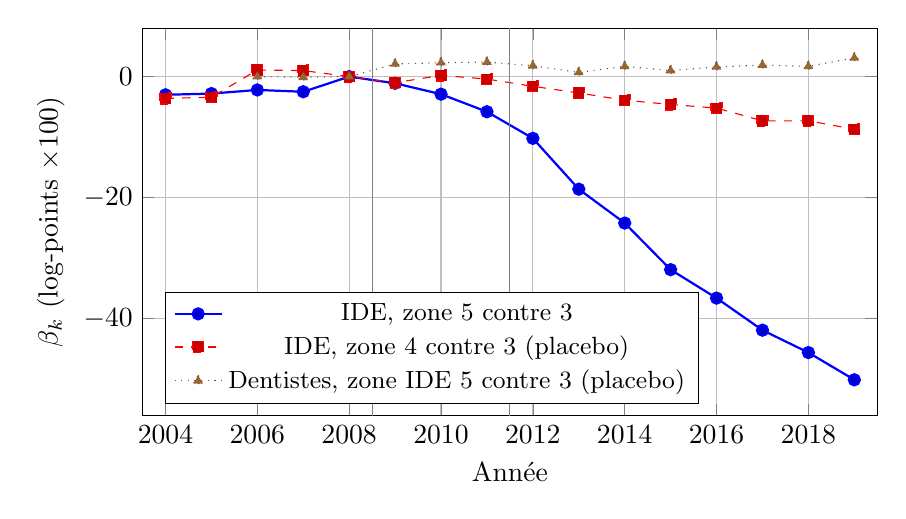
\begin{tikzpicture}
\begin{axis}[width=0.9\linewidth, height=6.5cm, xlabel={Année}, ylabel={$\beta_k$ (log-points $\times 100$)},
  xmin=2003.5, xmax=2019.5, ymin=-56, ymax=8, grid=major, legend pos=south west,
  xticklabel style={/pgf/number format/1000 sep={}}, legend style={font=\small}]
\addplot+[mark=*, thick] coordinates {(2004,-3.0) (2005,-2.8) (2006,-2.2) (2007,-2.5) (2008,0) (2009,-1.1)
  (2010,-2.9) (2011,-5.8) (2012,-10.2) (2013,-18.6) (2014,-24.2) (2015,-31.9) (2016,-36.6) (2017,-41.9)
  (2018,-45.6) (2019,-50.1)};
\addlegendentry{IDE, zone 5 contre 3}
\addplot+[mark=square*, dashed] coordinates {(2004,-3.6) (2005,-3.4) (2006,1.1) (2007,1.0) (2008,0) (2009,-1.0)
  (2010,0.2) (2011,-0.4) (2012,-1.6) (2013,-2.7) (2014,-3.9) (2015,-4.6) (2016,-5.2) (2017,-7.3) (2018,-7.3)
  (2019,-8.7)};
\addlegendentry{IDE, zone 4 contre 3 (placebo)}
\addplot+[mark=triangle*, dotted] coordinates {(2006,0.0) (2007,-0.1) (2008,0) (2009,2.1) (2010,2.3) (2011,2.4)
  (2012,1.8) (2013,0.7) (2014,1.7) (2015,1.0) (2016,1.6) (2017,1.9) (2018,1.7) (2019,3.1)};
\addlegendentry{Dentistes, zone IDE 5 contre 3 (placebo)}
\draw[gray] (axis cs:2008.5,-56) -- (axis cs:2008.5,8);
\draw[gray] (axis cs:2011.5,-56) -- (axis cs:2011.5,8);
\end{axis}
\end{tikzpicture}
\caption{Étude d'événement E1, référence 2008\mesure{}. Les traits verticaux encadrent la transition
2009--2011. Les quatre années d'avant sont au même niveau entre elles ($-2{,}2$ à $-3{,}0$) : c'est
2008 qui s'en écarte, ce que T1 rejette. Source : \texttt{did\_e1\_event\_study*.csv}.}
\label{a3-fig:es}
\end{figure}

\paragraph{Lecture.} L'écart entre les années 2004--2007 est faible : de $-\num{2.2}$ à
$-\num{3.0}$\mesure{} points par rapport à 2008. Il prend la forme d'un saut en 2008, pas d'une
tendance. Après 2011, l'écart se creuse de 5 à 8\mesure{}~points par an, sans plateau jusqu'en 2019
(figure~\ref{a3-fig:es}). Ce profil est compatible avec une régulation qui n'agit qu'au flux des
entrées, mais le protocole ne permet pas de conclure.

\paragraph{Analyses exploratoires (écrites après avoir vu T1).} Ces analyses ne valident rien.
\begin{itemize}
  \item En prolongeant la tendance linéaire des années 2004--2008 (\num{+0.64}\mesure{}~point par
        an), l'effet devient $\num{-36.4}$\derive{}. Avant 2009, la zone sur-dotée croissait plus vite :
        la violation joue contre l'effet.
  \item Avec la restriction $\Delta^{RM}(\bar M = 1)$ \citep{a3-rambachan2023}, chaque variation
        annuelle de la violation après 2008 est bornée par la plus grande variation annuelle d'avant,
        \num{2.5}\mesure{}~points. La violation en $t$ vaut donc au plus \num{2.5}\,$(t-2008)$,
        soit un biais d'au plus \num{18.6}\derive{}~points sur la moyenne 2012--2019. En élargissant l'IC de ce biais, on obtient
        $[\num{-52.7} ; \num{-7.9}]$\derive{}. Le signe tient. C'est une approximation (borne
        ajoutée à l'IC), et non l'inférence uniformément valide des auteurs.
  \item L'IRDES trouve un effet de même signe sur une autre série et une autre période
        \citep{a3-irdes270}.
\end{itemize}

\subsection{Niveau 3, E2 : marche et arrêt chez les kinés}
\begin{table}[h]
\centering\small
\begin{tabular}{@{}lccl@{}}
\toprule
Test & Estimation & Prédiction & Verdict \\
\midrule
Tendances parallèles 2005--2010 ($G = 26$) & $F(6, 20) = \num{1.47}$\mesure{}, $p = \num{0.24}$\mesure{} & $p \ge \num{0.10}$ & passe \\
Pente 2011--2014 (pts/an) & $\num{-2.4}$\mesure{} $[\num{-3.5} ; \num{-1.2}]$ & $< 0$ & confirmée \\
Pente 2014--2017 (pts/an) & $+\num{0.7}$\mesure{} $[\num{-0.7} ; \num{2.1}]$ & --- & --- \\
\textbf{Écart des pentes} ($G = 29$) & $\mathbf{+\num{3.1}}$\mesure{} $[\num{1.1} ; \num{5.1}]$ & $> 0$ & \textbf{confirmée} \\
\bottomrule
\end{tabular}
\caption{E2, kinés, zone sur-dotée contre intermédiaire, référence 2011.}\label{a3-tab:e2}
\end{table}
La zone sur-dotée décroche de 7\mesure{}~points pendant les deux ans et demi de régulation (2014 :
$\num{-7.0}$\mesure{}). Après l'annulation, elle cesse de décrocher (2017 : $\num{-4.4}$\mesure{}).
C'est la première prédiction pré-enregistrée sur un levier qui tient. Ce n'est pas encore une
validation du module, car $\theta$ n'a pas été pré-enregistré pour E2.

\subsection{Niveau 1 : premier passage confirmatoire}
La session de l'axe~2 a lancé le banc N1 sur le périmètre privé, après avoir inscrit ses
variantes\footnote{Rapport interne \texttt{v2/docs/lab/reports/2026-11-14-axe2-methodes.md}.}. La
variante par défaut obtient une MAPE de \num{8.68}\mesure{}~\%, contre \num{9.30}\mesure{}~\% pour la
tendance et \num{9.92}\mesure{}~\% pour la persistance. Elle gagne donc :
$\Delta = \num{-0.63}$\mesure{} $[\num{-0.97} ; \num{-0.27}]$. Le seul gain reproduit sur les deux
périmètres est le rétrécissement hiérarchique : $-\num{0.11}$\mesure{} $[\num{-0.21} ;
\num{-0.02}]$. La clause d'instabilité du protocole joue pour les dentistes : la variante par défaut
ne bat la naïve que sur 2\mesure{} origines sur 6. Aucune prévision n'est encore déposée pour 2027.

\subsection{Niveau 3, second test : au sein des bassins de vie (N7-A)}
Sur 135\mesure{} bassins de vie et 60\mesure{} départements, l'effet est de
$\num{-32.2}$\mesure{} $[\num{-37.2} ; \num{-27.3}]$. Le test de tendances échoue de nouveau
($F(4, 56) = \num{3.02}$, $p = \num{0.025}$\mesure{}), ainsi que le placebo de date ($+\num{2.6}$\mesure{}
$[\num{0.1} ; \num{5.1}]$). Les placebos dentistes ($+\num{0.6}$\mesure{}) et zone~4
($\num{-10.3}$\mesure{}, sous la moitié de l'effet) passent. Avant 2008, la zone sur-dotée gagnait
environ 1\mesure{}~point par an sur sa voisine intermédiaire ; après 2011, elle décroche de 6 à
8\mesure{}~points par an. \textbf{Design invalide : le levier IDE reste non validé.} Chez les kinés,
l'écart des pentes est de $+\num{3.3}$\mesure{} $[\num{0.8} ; \num{5.8}]$ points par an, mais le test de
tendances échoue à ce grain ($p = \num{0.059}$\mesure{}).

\subsection{Niveau 1 : stabilité entre origines (N7-B)}
\begin{table}[h]
\centering\small
\begin{tabular}{@{}lccc@{}}
\toprule
Estimateur (périmètre privé) & 2016 & 2018 & 2021 \\
\midrule
Variante par défaut & $+\num{0.10}$ égalité & $\num{-0.22}$ égalité & $\num{-1.22}$ gagne \\
Rétrécissement hiérarchique & $\num{-0.16}$ égalité & $\num{-0.43}$ égalité & $\num{-1.08}$ gagne \\
APC des sorties & $\num{-0.06}$ égalité & $\num{-0.16}$ égalité & $\num{-0.96}$ gagne \\
Rétention 60+ en tendance & $+\num{1.05}$ perd & $+\num{0.17}$ égalité & $\num{-1.25}$ gagne \\
\bottomrule
\end{tabular}
\caption{$\Delta$ MAPE (points) contre la meilleure naïve, $h = 5$, par origine\mesure{}. Extrait.}
\end{table}
Au périmètre privé, la victoire poolée de la variante par défaut repose sur l'origine 2021. Le
classement des estimateurs change presque complètement d'une origine à l'autre (τ de Kendall de
\num{0.07} à \num{0.29}\mesure{}). Sur l'ancien périmètre, la variante par défaut garde le même signe
aux trois origines.

\subsection{Niveau 5 : mondes simulés}
Le moteur est exact dans le monde à l'équilibre (erreur $< 10^{-13}$\mesure{}~\%). Il échoue dans deux
mondes :
\begin{itemize}
  \item \textbf{monde bruité} : 9 réplications sur 20 sous 1~\% d'erreur nationale à 15~ans, et une
        MAPE départementale de \num{10.2}\mesure{}~\% contre un plancher de Poisson de
        \num{5.7}\derive{}~\% ;
  \item \textbf{cohorte nombreuse} : les 60~ans et plus sont \emph{sous}-estimés de
        \num{34.5}\mesure{}~\% à 5~ans, contre la prédiction reprise de l'observatoire.
\end{itemize}
Les mondes à entrées croissantes, à saut d'entrées et à report du départ donnent le signe prédit
(20 réplications sur 20). Avec des entrées en hausse de 3~\% par an, l'ampleur atteint
$\num{-19.8}$\mesure{}~\%, au-delà de la tolérance autour de $-\num{12.4}$~\%. Une même cause explique
les deux échecs : la règle « rétention plafonnée à 1, excédent compté comme entrée » coupe le bruit
vers le bas et transforme en entrées tout excédent, y compris celui d'une cohorte qui passe.

\subsection{Niveau 6 et N7-C : prévision probabiliste}
Avec la bande empirique au même horizon (origine 2021 seulement), la persistance a le meilleur CRPS
(\num{0.0633}\mesure{}) ; la variante par défaut perd ($+\num{0.0098}$ $[\num{0.0037} ; \num{0.0161}]$).
Toutes les bandes sont trop étroites : l'intervalle « 80~\% » couvre de 56 à 70\mesure{}~\% des cas.
Avec la bande « pente d'erreur » (origines 2017--2021), tous les modèles battent la tendance
($\Delta \approx -\num{0.006}$\mesure{}), mais la bande est trop large : l'intervalle « 80~\% »
couvre environ 96\mesure{}~\%. Les tirages propres de l'APC (100 par cellule, moins que les 200
prévus par N6) font jeu égal avec la persistance ($+\num{0.0014}$ $[\num{-0.0033} ; \num{0.0068}]$),
mais leur intervalle « 80~\% » ne couvre que 54\mesure{}~\% des cas. Aucune de ces bandes n'est donc publiable sous son niveau nominal. La SBC passe
pour les cinq taux de rétention ($p$ de \num{0.14} à \num{0.94}\mesure{}) et échoue pour les entrées
($p \approx 3 \cdot 10^{-46}$\mesure{}, rang moyen \num{0.22}) : le bruit biaise les entrées vers le
haut, comme dans le monde bruité.

\subsection{Niveau 2 : DREES à 2050 (N2-A, N7-D)}
Faute d'une série ouverte des quotas 2016--2020, la reproduction de DD76 a été lancée avec des
entrées plates (moyenne 2016--2020), version affaiblie du protocole. Elle échoue : en 2050, le ratio
$N(t)/N(2020)$ est inférieur de \num{14.1} (dentistes), \num{15.0} (pharmaciens) et \num{17.4}\mesure{}~\%
(sages-femmes) à celui de DD76 ; les formes (creux, plateau) sont respectées. Une variante à entrées
par la filière dépasse DD76 de 14 à 15\mesure{}~\% (analyse exploratoire, qui utilise des inscrits
connus après 2020). L'ER~1319 part du même effectif 2021 que nous (\num{98631}\mesure{}) ; en 2050 nous
sommes \num{25.2}\mesure{}~\% en dessous, mais l'observé 2023 est déjà \num{5.9}\mesure{}~\% sous
l'ER~1319. Pour les dentistes, notre cible à entrées récentes (\num{81491}\mesure{} en 2050) dépasse
DD76 (\num{61800}) de \num{19691}. Les valeurs de Shapley attribuent \num{13056}\mesure{} à l'origine et
à la fenêtre, \num{11658}\mesure{} aux entrées récentes et $-\num{1877}$\mesure{} au périmètre ; le résidu
(16\derive{}~\%) passe le seuil. La variante par défaut, à entrées moyennes, donne
\num{61964}\mesure{}, proche de DD76.

\subsection{Niveau 2 : cas limites (N2-B)}
Sur le jumeau par défaut, au périmètre privé, les trois cas limites passent pour les cinq
professions. À l'origine, l'état reproduit l'observé (test faible, puisque l'état en est construit).
À 200 ans, l'effectif égale $Q \cdot C$ à $-\num{0.05}$ à $-\num{0.46}$\mesure{}~\% près ; l'écart vient
du plancher à zéro. Un état initial divisé par deux ne change rien. Une hausse de capacité de
formation n'agit qu'à $o + L_p + 1$\mesure{}, comme prévu.

\subsection{Niveau 4 : échelle fine}
Avec l'estimateur par défaut (total départemental de la cible, oracle, $\times$ part communale tenue),
le 80\textsuperscript{e} centile de l'erreur à 5~ans passe de 40--58\mesure{}~\% pour 3 à 5
professionnels à 4--15\mesure{}~\% au-delà de 200. La règle fixée d'avance donne
$N_{\min} = 51$\mesure{}, imposé par les kinés aux origines 2018 et 2020 ; il serait de 21 pour les
dentistes et les infirmiers seuls. La prédiction dérivée ($N_{\min} \ge 16$) tient. La bande
P10--P90 par classe est calibrée dans 14 classes sur 21\mesure{}. L'oracle retire l'erreur
départementale : l'erreur réelle est plus grande.

\subsection{N8 et dépôt 2027}
Avec la bande en $\sqrt h$, la variante par défaut couvre \num{49.2}\mesure{}~\% des cas à 50~\% et
\num{75.9}\mesure{}~\% à 80~\% : elle est calibrée, et elle bat la tendance en CRPS
($\num{-0.0045}$ $[\num{-0.0070} ; \num{-0.0020}]$\mesure{}). Le PIT reste chargé dans sa première
classe : les valeurs réelles sous la bande sont plus fréquentes que prévu. Les prévisions de
l'origine 2026 pour 2027, 2028 et 2030, avec leurs quantiles, sont déposées (empreinte
\texttt{ca036374d216}) et seront jugées à la publication du RPPS 2027.

\subsection{N9 : signe des boucles de rétroaction}
Avant qu'une boucle soit modélisée, N9 (gelé à 08:10, empreinte \texttt{96a39bc087bb}) teste son signe.
\begin{itemize}
  \item \textbf{B2, densité $\to$ installations nettes des moins de 40~ans}, par bassin de vie $\times$
        année (2014--2025). Le résultat est le solde d'installations pour \num{100000} habitants ; le
        régresseur est $\log(1 + D)$, densité décalée de deux ans. Contrôles : population, parts des
        moins de 15 et des plus de 65~ans, zonages 2012 et actuel ; effets fixes département et
        année. Signe attendu : $\beta < 0$.
  \item \textbf{B1, densité $\to$ rétention des 45--54~ans à 5~ans}, par département $\times$ année
        (RPPS, libéral et mixte). Contrôles : population, effectif de base ; effets fixes région et
        année. Signe attendu : $\beta > 0$.
  \item Pour les deux, variance robuste par département et placebo « densité des autres
        professions » : si le placebo a le même signe et au moins la moitié de l'effet, le verdict
        devient « non attribuable ».
\end{itemize}

\begin{table}[h]
\centering\small
\begin{tabular}{@{}llccl@{}}
\toprule
Boucle & Profession & $\beta$ [IC 95~\%] & Placebo & Verdict \\
\midrule
B2 & Infirmiers & $\num{-1.52}$ $[\num{-4.05} ; \num{1.01}]$ & $\num{-1.72}$ & nul \\
B2 & Kinés & $\num{-1.66}$ $[\num{-3.43} ; \num{0.11}]$ & $\num{-2.76}$ & nul \\
B2 & Dentistes & $+\num{0.17}$ $[\num{-0.05} ; \num{0.39}]$ & $\num{-0.45}$ & nul \\
B1 & Sages-femmes ($G = 15$) & $\num{-0.24}$ $[\num{-0.48} ; \num{0.01}]$ & $+\num{0.02}$ & nul \\
B1 & Dentistes & $+\num{0.04}$ $[\num{-0.03} ; \num{0.10}]$ & $+\num{0.05}$ & nul \\
B1 & Pharmaciens & $\num{-0.01}$ $[\num{-0.14} ; \num{0.11}]$ & $+\num{0.05}$ & nul \\
B1 & Kinés & $\num{-0.02}$ $[\num{-0.08} ; \num{0.03}]$ & $+\num{0.05}$ & nul \\
B1 & Infirmiers libéraux & $+\num{0.11}$ $[\num{0.05} ; \num{0.18}]$ & $\num{-0.00}$ & \textbf{confirmé} \\
\bottomrule
\end{tabular}
\caption{N9. B2 : installations nettes pour \num{100000} habitants par unité de $\log(1+D)$ (moyenne :
6,0 pour les IDE, 4,4 pour les kinés, 1,7 pour les dentistes) ; 20\,460 bassins de vie $\times$
années, 96 départements. B1 : $\log R$ par unité de $\log D$.\mesure{}}\label{a3-tab:n9}
\end{table}

\textbf{B2 n'est confirmé pour aucune profession.} Pour les IDE et les kinés, le point estimé a le
signe attendu, mais l'intervalle contient zéro. La densité des \emph{autres} professions pèse
autant ou plus : ce qui se voit ressemble à une attractivité générale du territoire, pas à une
saturation propre à la profession. Avec une densité décalée d'un an seulement, l'effet double
($\num{-2.3}$ et $\num{-2.7}$\mesure{}) : c'est le retour à la moyenne mécanique que le décalage de deux
ans devait écarter. \textbf{B1 est confirmé pour les seuls infirmiers libéraux} : une densité deux fois
plus forte va avec une rétention à 5~ans des 45--54~ans plus haute d'environ
8\derive{}~\% ($2^{0.113} - 1$). Ces relations restent écologiques, mesurées sur des soldes, et la
densité est elle-même le produit des installations passées : elles ne sont pas causales.

\subsection{N10 : le grain le plus fin dont la bande est calibrée}
« Fiable » est défini comme \emph{calibré} : la bande à 80~\% doit contenir la valeur observée dans
environ 80~\% des cas. N10 (gelé à 08:31, empreinte \texttt{d86d27c7a750}) le teste à trois grains
(commune, bassin de vie, EPCI), pour les IDE, les kinés et les dentistes, sur les origines
2014--2020. La bande est l'intervalle P10--P90 des erreurs passées du même estimateur, par classe de
taille. Un grain est fiable si toutes ses classes ont une couverture comprise entre 75 et 85~\%.

\textbf{Aucun grain infra-départemental n'est fiable}, pour aucune des trois professions et aucun des
quatre estimateurs. En moyenne, la couverture est proche du nominal (81 à 84\mesure{}~\% pour les IDE,
80 à 81 pour les kinés, 72 à 79 pour les dentistes). Par classe de taille, elle ne l'est pas : la bande
est trop large pour les très petites communes (94\mesure{}~\% pour les IDE de 1 ou 2
professionnels) et trop étroite au-delà de 50 à 100 professionnels (22 à 59\mesure{}~\%). La moyenne
est portée par la masse des petites communes. Le département reste donc le grain d'affichage des
projections, avec la bande en $\sqrt h$ de N8 ; à la commune, la carte montre l'observé. Le modèle
hiérarchique de l'axe~2 (K3), jugé sur ce même protocole, corrige l'essentiel de la sous-couverture
des grandes unités, mais ne passe à aucun grain : les bandes des IDE restent trop larges (85 à
91\mesure{}~\% dans les classes moyennes), celles des dentistes trop étroites (69 à 73\mesure{}~\%).
Le cas le plus proche est celui des kinés à l'EPCI, où une seule classe sur huit sort de l'intervalle
(73,0\mesure{}~\% pour 1 à 2 professionnels). Sa variante K4, inscrite avant passage, a été jugée selon un protocole gelé avant
qu'elle existe (N11, empreinte \texttt{4bf54ad0587a}) : elle devait passer N10 \emph{et} une origine
réservée (2021, $h = 4$). Elle échoue aux deux étapes, à tous les grains. Sur l'origine réservée, la simple
tendance des unités calibre toutes les classes des kinés au bassin de vie, alors qu'elle échoue N10 :
une seule origine favorable n'aurait rien prouvé. Une troisième variante, K5, jugée selon un protocole gelé avant ouverture de ses fichiers (N12,
origine réservée 2022, $h = 3$), échoue elle aussi aux deux étapes : ses bandes sont devenues trop
étroites (59 à 66\mesure{}~\% de couverture pour les infirmiers à l'EPCI et au bassin de vie). Aucune des
trois variantes n'a calibré un grain plus fin que le département.

\section{Validation et menaces à la validité}\label{a3-sec:menaces}
\subsection{Cas d'étude : des tests vrais par construction}
Le jumeau a subi deux revues adversariales\footnote{Rapports internes
\texttt{2026-11-14-revue-adversariale-axe0.md} et \texttt{-v2.md}.}. Neuf agents en lecture seule
les ont menées selon trois angles. Pour chaque angle, les deux constats les plus graves ont été
soumis à un agent chargé de les réfuter en exécutant le code.
\begin{itemize}
  \item \textbf{Première revue :} 6\mesure{} constats soumis à réfutation, 6 confirmés, dont
        4 bloquants. Le critère « plug-in » écrivait le module factice dans un dossier temporaire :
        son contrôle « aucun fichier modifié » ne pouvait pas échouer. Le critère de conservation
        comparait le registre des flux à une variation qu'il stockait lui-même, si bien que son
        résidu de $3 \cdot 10^{-11}$ ne mesurait que l'arrondi. L'agrégation comparait les communes
        à des regroupements des mêmes lignes ; face au RPPS, l'écart est de
        $-\num{5.4}$\mesure{}~\% pour les kinés en 2025.
  \item \textbf{Seconde revue :} 6\mesure{} constats confirmés, soit 4 défauts bloquants
        distincts. Le test du levier retraite comparait le jumeau à la version~1, qui portait le
        même masque fautif : il ne pouvait pas voir le défaut (+41\mesure{}~\% d'effet à 2050 pour un
        report de 2~ans). Une correction en avait aussi introduit un nouveau : un scénario passé à
        \texttt{trajectory} remplaçait le scénario de base ($-\num{15.2}$\mesure{}~\%).
\end{itemize}
\textbf{Leçon pour nos protocoles.} Un test qui compare un objet à une copie de lui-même, ou qui
mesure une identité, passe par construction. Nos protocoles s'en gardent de quatre façons :
\begin{itemize}
  \item N5 interdit au générateur de partager du code ou une hypothèse avec l'estimateur ;
  \item N2 compare à une source extérieure, DD76, et pas à la version~1 ;
  \item N3 ajoute des placebos qui \emph{peuvent} échouer ;
  \item la règle de mutation de l'axe~0 (réintroduire le défaut et vérifier que le test échoue)
        est la contrepartie, dans le code, du pré-enregistrement.
\end{itemize}

\subsection{Menaces propres à nos résultats}
\begin{itemize}
  \item \textbf{Date du zonage.} Le jeu Atlasanté porte des codes de régions antérieurs à 2016 et
        des métadonnées de 2014 : il est \emph{probablement} le zonage de 2012. S'il s'agissait
        d'une révision de 2014 fondée sur des densités postérieures à 2012, le traitement serait en
        partie choisi sur le résultat. E1 et E2 tomberaient ensemble.
  \item \textbf{Un verdict qui tient à un seuil.} Le test donne $p = \num{0.043}$ pour un seuil de
        \num{0.10}. Ce seuil était fixé d'avance, et nous ne le changeons pas. Un second test, par
        exemple $\Delta^{RM}$ avec $\bar M$ fixé d'avance, devra être pré-enregistré et déclaré
        comme tel.
  \item \textbf{Retour à la moyenne.} La zone~4 décroche aussi, de $-\num{4.2}$\mesure{}~points en
        moyenne. Jusqu'à environ un septième\derive{} de l'effet IDE peut venir de la convergence
        des zones denses.
  \item \textbf{Dates d'effet.} Elles viennent de sources secondaires. L'absence de régulation
        dentaire avant 2025 et la date du rezonage infirmier sont supposées.
  \item \textbf{Contamination de N1.} Les cibles 2023 et 2026 avaient déjà été vues par K1. Seul le
        dépôt de 2027 est propre. Le bootstrap par département ignore aussi la corrélation entre
        origines, si bien que l'IC est probablement trop étroit\suppose{}.
  \item \textbf{Ordre de gel.} N5 a été gelé après le lancement de N3. Les deux niveaux ne partagent
        ni données ni seuil.
  \item \textbf{Seconds tests.} N7-A est un second essai sur le même levier : la protection du
        pré-enregistrement est entamée. Il échoue de toute façon.
  \item \textbf{Forme affaiblie de N2.} Faute de série de quotas, les entrées de DD76 ne sont pas
        reproduites ; l'échec de N2-A mêle l'écart de moteur et l'écart d'hypothèse.
  \item \textbf{Seuils choisis.} Les seuils de 3~\% (N2), 25~\% (N4) et $p \ge 0{,}10$ (N3) sont des
        choix argumentés, pas des dérivations.
\end{itemize}

\section{Reproductibilité}\label{a3-sec:repro}
Toutes les commandes se lancent depuis la racine du dépôt. \texttt{scipy} est ajouté à la volée,
sans toucher au \texttt{pyproject.toml} partagé.
\begin{verbatim}
# N3, N3 exploratoire, auto-test, N7-A, N7-B, N6 et N7-C, N5 et SBC, N2
PYTHONPATH=v2 uv run --with scipy python -m validation.did
PYTHONPATH=v2 uv run --with scipy python -m validation.did_explore
PYTHONPATH=v2 uv run --with scipy python -m validation.selftest
PYTHONPATH=v2 uv run --with scipy python -m validation.did_commune
PYTHONPATH=v2 uv run --with scipy python -m validation.stability prive
PYTHONPATH=v2 uv run --with scipy python -m validation.probabilistic
PYTHONPATH=v2 uv run --with scipy python -m validation.worlds all
PYTHONPATH=v2 uv run --with scipy python -m validation.dd76
PYTHONPATH=v2 uv run --with scipy python -m validation.limits_twin
PYTHONPATH=v2 uv run --with scipy python -m validation.fine_scale_run
PYTHONPATH=v2 uv run --with scipy python -m validation.depot
PYTHONPATH=v2 uv run --with scipy python -m validation.boucles
# empreintes des protocoles gelés
shasum -a 256 v2/validation/preregistered/*.md
\end{verbatim}
\begin{itemize}
  \item \textbf{Graines} : \texttt{20261114} pour tous les bootstraps ; \texttt{20261114}~+~$r$ pour
        la réplication $r$ des mondes simulés.
  \item \textbf{Données} :
        \begin{itemize}
          \item \texttt{data/processed/stock\_commune.parquet} (CartoSanté, extrait le 2026-11-13) ;
          \item \texttt{v2/validation/raw/zonage\_conv\_c987.geojson} (Atlasanté, extrait le
                2026-11-14 ; libre réutilisation en citant la source et la date) ;
          \item \texttt{data/processed/stock.parquet} (RPPS, publié le 2026-07-02).
        \end{itemize}
  \item \textbf{Sorties} : \texttt{v2/validation/out/}.
  \item \textbf{Code} : les modules Python du dossier \texttt{v2/validation/} (un par niveau,
        plus le registre des estimateurs).
  \item \textbf{Autres données} : tables communales de l'axe~4
        (\texttt{v2/data/processed/}) ; projections DREES des infirmières 2024 (data.drees, export
        CSV, extrait le 2026-11-14).
  \item \textbf{Version} : le dépôt n'était pas encore versionné au moment des calculs ; les
        empreintes des protocoles tiennent lieu de version.
\end{itemize}

\section{Conclusion}
La validation d'un jumeau à 2050 ne peut pas être un seul backtest. Nous l'avons découpée en dix
protocoles, gelés avant leurs résultats et appliqués tels quels. Presque tous les tests qui pouvaient
échouer ont échoué, et c'est l'information principale :
\begin{itemize}
  \item le levier IDE a un effet grand et constant, mais deux designs fixés d'avance refusent de le
        valider ;
  \item la précision par département n'est acquise que sur une origine ;
  \item le moteur par défaut confond bruit, passage de cohorte et entrées ;
  \item seule la bande en $\sqrt h$ est calibrée, sous réserve du dépôt 2027 ;
  \item à 2050, l'hypothèse d'entrées domine tout, de $-15$ à $+15$\mesure{}~\% autour de DD76.
\end{itemize}

\paragraph{Ce que cela change.}
\begin{itemize}
  \item Aucun chiffre 2050 n'est citable. Seule la bande en $\sqrt h$ peut être affichée sous son niveau
        nominal, et sous 51 professionnels une projection communale ne s'affiche pas sans elle.
  \item Les axes 0 et 2 doivent séparer les entrées de la rétention.
  \item L'axe~5 doit vérifier la calibration de sa composante (b), linéaire en $h$.
  \item La boucle densité $\to$ installations (B2) n'a pas de signe établi : l'axe~2 ne l'ajoute pas comme
        covariable confirmée. La boucle densité $\to$ départs (B1) n'est confirmée que pour les
        infirmiers libéraux, au département.
  \item Le niveau d'entrées de référence (moyenne de fenêtre ou années récentes) est une décision qui
        revient à l'équipe : il fait passer les dentistes en 2050 de \num{62000} à \num{81000}\mesure{}.
\end{itemize}

\paragraph{Questions ouvertes, avec leur coût (temps de travail estimé).}
\begin{itemize}
  \item Troisième test du levier IDE (contrôle synthétique par bassin de vie) : environ 1~h.
  \item Série ouverte des quotas 2016--2020 pour une reproduction fidèle de DD76 : environ 45~min.
  \item Dater le jeu Atlasanté contre un arrêté ARS de 2012 : environ 30~min.
  \item $N_{\min}$ avec la projection départementale réelle au lieu de l'oracle : environ 15~min.
  \item Score du dépôt 2027 (juillet 2027) : environ 15~min.
\end{itemize}



\part{Axe 4 --- données}
\noindent\textit{Article d'origine : « Le secteur public était déjà dans les fichiers : séparer public et privé, dater les réformes, coder le zonage, fixer le grain communal et observer les flux d'un jumeau numérique de l'offre de soins » (\texttt{v2/papers/axe4-donnees/}).}

\begin{quote}\small\textbf{Résumé de l'axe.} Le jumeau numérique de l'offre de soins projette jusqu'en 2050 l'effectif « libéral » de cinq professions
(sages-femmes, chirurgiens-dentistes, pharmaciens, masseurs-kinésithérapeutes, infirmiers). Ici, « libéral »
désigne le secteur privé, lucratif ou non : tout employeur public est exclu. Or le stock DREES utilisé jusqu'ici
ne séparait pas public et privé chez les salariés. La sortie 2026 n'était donc connue qu'en fourchette, de
\num{12475} à \num{26428} sages-femmes. Nous montrons que la séparation est déjà dans les fichiers ouverts de la
DREES : ils croisent département, secteur d'activité, mode d'exercice, âge et sexe. Les salariés des secteurs
mixtes sont répartis à l'aide du répertoire FINESS. La fourchette des sages-femmes devient
\num{12059}--\num{13331}\mesure{} : sa largeur baisse de 91\,\%\derive{}. Les infirmiers sont séparés sans
ambiguïté : \num{277788} privés en 2023\mesure{}. Nous livrons aussi un registre de 30 événements datés et
sourcés, et le zonage conventionnel de \num{34919} géocodes pour quatre professions. Chaque table est contrôlée
contre un total connu. Le registre est confirmé sur un cas : l'année sans diplômés en kinésithérapie (2018) se
lit dans le stock, avec \num{-34.6}\,\% de moins de 25 ans\mesure{}. Le zonage reproduit le périmètre dentaire
publié, soit 97 géocodes et 4,8\,\% de la population\mesure{}. Enfin, l'Annuaire Santé rend les cinq
professions observables à la commune. Mais la médiane des effectifs privés par commune est nulle. Le grain
projetable est donc le bassin de vie ou l'EPCI pour les infirmiers, et le département pour les dentistes et les
sages-femmes. Ce même fichier montre que 24\,\% des dentistes et 32\,\% des kinésithérapeutes actifs n'ont pas
de diplôme d'État français\mesure{}. Pour le modèle de choix d'installation, nous construisons un substitut
d'installations nettes par commune (2012--2025), l'historique des officines (2004--2025 ; 20\,083 en 2025) et une
table d'attributs communaux ; le substitut ne voit qu'une fraction de l'année blanche des kinésithérapeutes. Limite : les infirmiers n'entrent dans le jumeau que sous l'hypothèse d'un
secteur indépendant de l'âge et du sexe, testée sur le sexe seulement.\end{quote}

\section{Introduction}
Le projet simule des politiques nationales sur un jumeau de l'offre de soins. Chaque politique y est un
réglage d'hyperparamètres sourcés. La sortie est l'effectif « libéral » de cinq professions, à toute échelle
jusqu'à la commune. Il s'agit de la définition du projet, qui diffère de celle des sources : le secteur privé,
lucratif ou non, y compris les pharmaciens adjoints d'officine, les salariés des cliniques et l'industrie. Tout
employeur public en est exclu : hôpital public, PMI, Éducation nationale, EHPAD publics, centres municipaux.

Trois lacunes de données bloquaient ce cadrage :
\begin{enumerate}
  \item le stock ne séparait pas public et privé dans « salarié hospitalier » et « autre salarié ». La sortie
  2026 n'était donc connue qu'en fourchette : \num{12475}--\num{26428} sages-femmes et
  \num{65344}--\num{75335} pharmaciens\mesure{} ;
  \item les ruptures des séries (formation, diplômés, installation) n'étaient rattachées à aucune réforme datée ;
  \item la régulation de l'installation, qui s'applique par commune, n'existait dans le jumeau que sous forme de
  zones illustratives.
\end{enumerate}

\paragraph{Contributions.}
\begin{itemize}
  \item Une séparation public / privé par profession, mode, département, âge, sexe et année (2012--2026). Elle
  donne pour chaque sortie une fourchette resserrée et une valeur centrale (section~\ref{a4-sec:res-secteur}).
  \item Un registre de 30 événements datés, chacun avec sa source ouverte. Il comprend deux ruptures de données,
  dont un artefact de fichier qui passait pour une réforme (section~\ref{a4-sec:res-evenements}).
  \item Le zonage conventionnel de \num{34919} géocodes pour quatre professions, sur deux millésimes, avec le
  statut lu par le module de régulation (section~\ref{a4-sec:res-zonage}).
  \item Un inventaire des sources ouvertes à la commune. Il comble quatre trous : Marseille, sages-femmes,
  pharmaciens et infirmiers par âge et sexe. Il donne aussi le grain projetable par profession
  (section~\ref{a4-sec:res-grain}).
  \item Des flux communaux pour le modèle de choix d'installation : un substitut d'installations nettes, les
  ouvertures et fermetures d'officines, une table d'attributs communaux et l'archivage de l'Annuaire Santé
  (section~\ref{a4-sec:res-flux}).
\end{itemize}

\section{Travaux existants}
La DREES publie chaque année les effectifs au 1\textsuperscript{er} janvier, à partir du RPPS
\citep{a4-drees2026demo}. La feuille « Lisez-moi » documente le croisement par département, secteur d'activité,
mode d'exercice, âge et sexe. Les kinésithérapeutes y sont comptés au RPPS depuis 2017, et à partir d'ADELI
avant cette date \citep{a4-drees2020er1159}. Pour les infirmiers, la DREES croise deux sources : la Base Tous Salariés
(Insee) pour les salariés, le SNDS pour les libéraux \citep{a4-dreesbts2026}. Le répertoire FINESS décrit les
établissements et le statut juridique de leurs gestionnaires \citep{a4-finessEt2026,a4-finessEj2026}.

Le zonage conventionnel est arrêté par les ARS et diffusé par CartoSanté \citep{a4-cartosante2026}. Une génération
antérieure est publiée par le catalogue Atlasanté \citep{a4-atlasante2014zonage}. Les règles qui s'y attachent
viennent des avenants aux conventions nationales :
\begin{itemize}
  \item infirmiers \citep{a4-ameliIde} ;
  \item sages-femmes \citep{a4-ameliSf} ;
  \item kinésithérapeutes \citep{a4-ameliMk}, dont la régulation a été annulée en 2014 par le Conseil d'État
  \citep{a4-ce2014mk} ;
  \item chirurgiens-dentistes \citep{a4-arspaca2025cd}.
\end{itemize}
L'Agence du numérique en santé publie une extraction en libre accès du RPPS, remplacée à chaque mise à jour \citep{a4-ans2026annuaire}.
Elle donne la commune de chaque activité, mais ni l'âge ni d'archive. L'Insee publie la composition communale
des bassins de vie 2022 \citep{a4-insee2026bv}.
Nous n'avons pas trouvé de travail qui exploite le croisement secteur~$\times$~mode du fichier DREES pour isoler
le secteur privé au sens large.

\section{Données}
\begin{table}[h]
\centering\small
\begin{tabular}{@{}p{4.2cm}p{3.1cm}p{4.3cm}p{3.2cm}@{}}
\toprule
Jeu & Producteur, millésime & Grain & Usage \\
\midrule
Démographie des PS depuis 2012 \citep{a4-drees2026demo} & DREES, 2026-07-02 & dép.\ $\times$ secteur (8--12) $\times$ mode (4) $\times$ âge (10) $\times$ sexe, 2012--2026 & SF, CD, PH, MK \\
Infirmières salariées BTS, libérales SNDS \citep{a4-dreesbts2026} & DREES / Insee, 2026-07-02 & dép.\ $\times$ secteur (6), sans croisement âge ou sexe ; 2013--2023 & IDE \\
FINESS établissements et entités juridiques \citep{a4-finessEt2026,a4-finessEj2026} & Ministère, au 2026-05-04 & établissement, catégorie, statut juridique & parts privées \\
CartoSanté \texttt{zonage\_conv} \citep{a4-cartosante2026} & CNAMTS--ARS, extrait 2026-11-14 & commune COG 2026, arrondissements PLM & zonage actuel \\
Atlasanté c987d0e2 \citep{a4-atlasante2014zonage} & ARS Aquitaine, 2014 & commune (\num{36700}) & zonage « 2012 » (déduit : codes région d'avant 2016 ; la fiche ne date pas la génération) \\
Découpage administratif \citep{a4-geoapi2026} & Etalab, 2026-11-14 & commune, population légale & contrôles \\
\bottomrule
\end{tabular}
\caption{Jeux de données. Tous sont ouverts. Les fichiers FINESS pèsent \SI{35.8}{\mega\byte} et
\SI{11.9}{\mega\byte}\mesure{}, le zonage environ \SI{1.6}{\mega\byte} par profession\mesure{}.}
\label{a4-tab:donnees}
\end{table}

\paragraph{Contrôles d'entrée.}
\begin{itemize}
  \item La somme des cellules détaillées (dép.~$\times$ secteur $\times$ mode $\times$ âge $\times$ sexe) égale
  le total France du fichier, à 0\,\% près\mesure{} pour les sages-femmes, les dentistes, les pharmaciens et
  ADELI.
  \item Les kinésithérapeutes RPPS font exception : 0,22\,\% d'écart au plus\mesure{}, atteint en 2026 (0,18\,\% en
  2017, 0,08\,\% en 2018). L'écart est interne au fichier source : en 2017, la somme des cellules départementales
  vaut \num{84599} contre \num{84449} pour le total France\mesure{} ; la feuille « Lisez-moi » prévient que
  certains totaux peuvent différer de la somme.
  \item Pour le BTS, l'écart est d'au plus 0,009\,\%\mesure{}.
\end{itemize}

\section{Méthode}
\subsection{Classement public / privé}
Soit $N_{p,s,m,d,a,x,t}$ l'effectif de la profession $p$ dans le secteur $s$, le mode $m$, le département $d$,
l'âge $a$, le sexe $x$ et l'année $t$. Chaque cellule reçoit une part privée $\pi \in [0,1]$ :
\begin{itemize}
  \item libéral ou mixte : $\pi = 1$, quel que soit le secteur. C'est la définition du projet, dans laquelle
  les mixtes sont inclus.
  \item Salarié dont le secteur est sans ambiguïté : $\pi = 0$ pour l'hôpital public ; $\pi = 1$ pour les
  établissements ESPIC et privés lucratifs, l'officine, les laboratoires, le médicament et les cabinets.
  \item Salarié d'un secteur mixte (centre de santé, prévention, médico-social, « autre ») : $\pi$ est inconnu.
  Il est borné par $[0,1]$ et prend une valeur centrale $\hat\pi$.
\end{itemize}
La sortie privée est alors encadrée et centrée :
\begin{equation}
N^{\min}_{p,t} = \sum_{\text{sûr privé}} N, \qquad
N^{\max}_{p,t} = N^{\min}_{p,t} + \sum_{\text{ambigu}} N, \qquad
\hat N_{p,t} = \sum \hat\pi\, N .
\end{equation}

\subsection{Parts centrales par FINESS}
La valeur $\hat\pi$ est la part d'établissements de la catégorie FINESS correspondante dont l'entité juridique est
privée :
\begin{itemize}
  \item statuts juridiques 47 à 99 : privé (mutuelles, associations, fondations, sociétés) ;
  \item statuts 1 à 39 : public ;
  \item statuts 40 à 46, organismes de sécurité sociale : comptés publics, comme administrations de sécurité
  sociale.
\end{itemize}
Les catégories retenues sont :
\begin{itemize}
  \item centres de santé (124) ; pour les dentistes, les centres dont la raison sociale contient « DENT » ;
  \item PMI et planification (223, 228) ;
  \item EHPAD (500) ;
  \item handicap médicalisé (182, 183, 186, 190, 255, 437, 448).
\end{itemize}
« Autre secteur », et « prévention et établissement de santé » chez les pharmaciens, n'ont pas de proxy :
$\hat\pi = 0{,}5$\suppose{}. Une exception est mesurée : les sages-femmes salariées en « prévention » sont
classées publiques, car la DREES compte \num{1423} sages-femmes en PMI au 31/12/2024 pour \num{1383} en
« prévention » au RPPS 2026\mesure{}.

\paragraph{Infirmiers.} Le BTS sépare déjà public et privé en trois paires : hôpital, médico-social, autre. Les
libéraux SNDS sont privés. Aucune ambiguïté n'est donc introduite. Le BTS ne croise pas le secteur avec l'âge ou
le sexe, et la table infirmiers n'a que le grain département~$\times$ secteur.

\subsection{Registre d'événements}
Chaque ligne de \texttt{v2/data/events.csv} est un texte ou un fait observé. Elle porte ces champs :
\texttt{id}, \texttt{date\_effet}, \texttt{profession}, \texttt{flux\_touche} (capacité de formation, durée des
études, diplômés, installation, régulation, compétences, autre), \texttt{type}, \texttt{description},
\texttt{source}, \texttt{millesime} et \texttt{confiance}.
\begin{itemize}
  \item Chaque URL a été ouverte, et le fait lu sur la page.
  \item \texttt{verifie} : date et fait lus sur la source. \texttt{partiel} : une partie de la date ou du chiffre
  est déduite, et la description le dit.
  \item Quand seule l'année est connue, la date retenue est la rentrée (1\textsuperscript{er} septembre) ou la fin
  d'année universitaire.
\end{itemize}

\subsection{Zonage et statut}
Le statut lu par le module de régulation se déduit de la classe ARS :
\begin{itemize}
  \item Statut \texttt{remplacement\_seul} : classes « sur-dotée » (ancien zonage) et « non prioritaire »
  (nouveau zonage). Le conventionnement n'y est possible qu'en remplacement d'un départ.
  \item Très sous-dotée ou sous-dotée : \texttt{incitation}.
  \item Les autres classes : \texttt{autre}.
\end{itemize}
Le référentiel \texttt{arm2026} remplace Paris, Lyon et Marseille par leurs 45 arrondissements, zonés à ce niveau.

\section{Résultats}
\subsection{Séparation public / privé}\label{a4-sec:res-secteur}
\begin{table}[h]
\centering\small
\setlength{\tabcolsep}{4pt}
\begin{tabular}{@{}lrrrrrr@{}}
\toprule
Profession & Année & Effectif & Ancienne & Min & Centrale & Max \\
 & & & fourchette & & & \\
\midrule
Sages-femmes & 2026 & \num{26428} & \num{12475}--\num{26428} & \num{12059} & \num{12819} & \num{13331} \\
Pharmaciens  & 2026 & \num{75335} & \num{65344}--\num{75335} & \num{60005} & \num{63612} & \num{67219} \\
Dentistes    & 2026 & \num{48690} & \num{48143}--\num{48690} & \num{40784} & \num{47349} & \num{47894} \\
Kinés        & 2026 & \num{111141} & \num{98348}--\num{111237} & \num{98828} & \num{101951} & \num{103986} \\
Infirmiers   & 2023 & \num{607644} & --- & \num{277788} & \num{277788} & \num{277788} \\
\bottomrule
\end{tabular}
\caption{Effectif « libéral » (= privé), France entière. Min, max et effectif sont mesurés\mesure{} ; la centrale
dépend des parts FINESS (mesurées\mesure{}) et de deux secteurs supposés à 0,5\suppose{} (« autre secteur » ; « prévention et établissement de santé » des pharmaciens), soit 5 cellules profession $\times$ secteur. Pour les infirmiers, le
total additionne BTS et SNDS (double compte possible, voir section~\ref{a4-sec:menaces}).}
\label{a4-tab:fourchettes}
\end{table}

La largeur de la fourchette baisse de 91\,\% pour les sages-femmes (de \num{13953} à \num{1272}), de 60\,\% pour
les kinésithérapeutes et de 28\,\% pour les pharmaciens\derive{}.

\paragraph{Pharmaciens hospitaliers.} Le RPPS place 16,6\,\% des pharmaciens salariés hospitaliers dans le privé
(19,8\,\% au plus)\mesure{}. La SAE en compte 29,4\,\% et l'Ordre 28,6\,\% (mesures de l'axe~1). Nous gardons
la centrale du RPPS, qui est croisée par département, âge et sexe. La variante SAE ajoute \num{1116} pharmaciens
privés\derive{} (\num{63612} $\rightarrow$ \num{64728}), dans la fourchette. L'écart n'est pas réconcilié.

\paragraph{Les anciennes bornes basses n'étaient pas des minima.} Elles comptaient tout « autre salarié » comme
privé, PMI et centres municipaux compris. C'est pourquoi le minimum baisse pour les sages-femmes et les
pharmaciens. Pour les dentistes, la fourchette s'élargit. Les \num{6694} dentistes salariés des centres de santé
sont désormais ambigus\mesure{}, mais leur part centrale est de 0,963\mesure{} : 96\,\% des \num{1299} centres
« dentaires » ont un gestionnaire privé.

\begin{table}[h]
\centering\footnotesize
\begin{tabular}{@{}llrrl@{}}
\toprule
Profession & Secteur & Effectif 2026 & $\hat\pi$ & Source de $\hat\pi$ \\
\midrule
Pharmaciens & Autre secteur & \num{5805} & 0,50\suppose & --- \\
Pharmaciens & Prévention et étab.\ de santé & \num{1409} & 0,50\suppose & --- \\
Dentistes & Centre de santé & \num{6694} & 0,963\mesure & FINESS, \num{1299} centres \\
Kinés & Étab.\ sanitaire et social & \num{2200} & 0,696\mesure & FINESS, \num{13407} étab. \\
Kinés & Autre secteur & \num{2524} & 0,50\suppose & --- \\
Sages-femmes & Autre secteur & \num{796} & 0,50\suppose & --- \\
\bottomrule
\end{tabular}
\caption{Origine de l'ambiguïté restante : salariés des secteurs mixtes, 2026 (lignes de plus de 500 personnes).}
\label{a4-tab:ambigu}
\end{table}

\begin{figure}[h]
\centering
\begin{tikzpicture}
\begin{axis}[width=0.85\textwidth,height=6cm,xlabel={Année (au 1\textsuperscript{er} janvier)},
  ylabel={Sages-femmes « libérales » (privé)},xmin=2012,xmax=2026,
  x tick label style={/pgf/number format/1000 sep=},
  y tick label style={/pgf/number format/1000 sep={\,}},
  legend pos=north west,legend style={font=\small}]
\addplot[name path=max,draw=none,forget plot] coordinates {(2012,7472) (2013,8064) (2014,8548) (2015,9097) (2016,9728) (2017,10140) (2018,10425) (2019,10685) (2020,11031) (2021,11452) (2022,11767) (2023,12122) (2024,12572) (2025,12885) (2026,13331)};
\addplot[name path=min,draw=none,forget plot] coordinates {(2012,6839) (2013,7675) (2014,8127) (2015,8704) (2016,9338) (2017,9760) (2018,10024) (2019,10255) (2020,10524) (2021,10707) (2022,10962) (2023,11238) (2024,11510) (2025,11706) (2026,12059)};
\addplot[gray!30] fill between[of=max and min];
\addlegendentry{min--max (secteurs mixtes)}
\addplot[thick,black,mark=*,mark size=1.2pt] coordinates {(2012,7249) (2013,7914) (2014,8388) (2015,8945) (2016,9577) (2017,9994) (2018,10273) (2019,10522) (2020,10843) (2021,11152) (2022,11438) (2023,11768) (2024,12142) (2025,12407) (2026,12819)};
\addlegendentry{centrale (FINESS)}
\end{axis}
\end{tikzpicture}
\caption{Sages-femmes du secteur privé, France entière, 2012--2026\mesure{}. L'ancienne fourchette 2026
(\num{12475}--\num{26428}) dépasserait le haut du graphique.}
\label{a4-fig:sf}
\end{figure}

Les séries existent pour chaque année et chaque département. La largeur médiane de la fourchette par département,
dernière année, va de 3,6\,\% de l'effectif (sages-femmes) et 4\,\% (kinésithérapeutes) à 9\,\% (dentistes,
pharmaciens)\mesure{}.

\subsection{Registre d'événements}\label{a4-sec:res-evenements}
Le registre compte 30 événements entre 2009 et 2028\mesure{} : 24 \texttt{verifie} et 6 \texttt{partiel}, après
l'audit des sources de l'axe~1. Deux lignes, la loi de 2023 et le décret de 2024 sur la maïeutique, décrivent le
même choc : elles sont marquées pour ne pas être appliquées deux fois.
\begin{table}[h]
\centering\small
\begin{tabular}{@{}lrp{10.5cm}@{}}
\toprule
Flux touché & N & Exemples (date d'effet) \\
\midrule
Régulation de l'installation & 11 & IDE 18/04/2009, 27/05/2012 \citep{a4-ameliIde} ; MK 15/07/2012, annulée le 17/03/2014 \citep{a4-ce2014mk}, puis 01/07/2018 et avenant~7 (2023) \citep{a4-ameliMk} ; SF 15/09/2012 \citep{a4-ameliSf} ; CD 01/01/2025 \citep{a4-arspaca2025cd} \\
Capacité de formation & 7 & numerus apertus, rentrée 2020 \citep{a4-loiotss2019} ; objectifs pluriannuels 2021--2025 et 2026--2030 ; 8 sites d'odontologie à la rentrée 2022 \\
Durée des études & 4 & MK : 3 à 4 ans en IFMK, rentrée 2015 \citep{a4-arretemk2015} ; SF : 6 ans, entrée en 2\textsuperscript{e} année à partir de 2024 \\
Diplômés & 2 & MK : année blanche 2018 \citep{a4-drees2020er1159} ; SF : (quasi) aucune diplômée en 2027-28 (déduit) \\
Compétences & 3 & IPA (2018) ; vaccination en officine (2019, 2023) \\
Installation (officines) & 1 & seuils de population (ordonnance 2018-3) \\
Données & 2 & passage ADELI $\rightarrow$ RPPS des MK en 2017 \citep{a4-drees2020er1159} ; artefact des inscrits 2025-26 \\
\bottomrule
\end{tabular}
\caption{Événements par flux touché. Liste complète, sources et fiches : \texttt{v2/data/events.csv},
\texttt{v2/docs/lab/fiches/data-ev-*.md}.}
\label{a4-tab:evenements}
\end{table}

\paragraph{Le saut d'inscrits 2025 est un artefact.} Le fichier des inscrits 2025-26 compte \num{2083} étudiants
en 2\textsuperscript{e} année d'odontologie\mesure{}, contre environ \num{1550} les années précédentes. Une seule
ligne explique le saut : l'Université Paris Cité, avec 683 inscrits\mesure{}, contre 188 à 215 entre 2020 et 2024
et 193 en 3\textsuperscript{e} année. Le fichier compilé de l'équipe donne \num{1588} au national, dans la tendance
(\num{1546} en 2024). Le registre enregistre donc ce saut comme une rupture de données, pas comme une réforme.

\subsection{Zonage par commune}\label{a4-sec:res-zonage}
\begin{table}[h]
\centering\small
\begin{tabular}{@{}lrrrr@{}}
\toprule
Profession & Remplacement seul & Incitation & Autre & Non renseigné \\
\midrule
Sages-femmes & \num{1471} \;(12,3\,\%) & \num{11862} \;(17,4\,\%) & \num{21562} \;(70,3\,\%) & 24 \\
Dentistes & 97 \;(4,8\,\%) & \num{26769} \;(44,4\,\%) & \num{8027} \;(50,8\,\%) & 26 \\
Kinés & \num{2836} \;(27,4\,\%) & \num{18840} \;(29,8\,\%) & \num{13241} \;(42,8\,\%) & 2 \\
Infirmiers & \num{4786} \;(27,6\,\%) & \num{5690} \;(15,3\,\%) & \num{24441} \;(57,0\,\%) & 2 \\
\bottomrule
\end{tabular}
\caption{Zonage actuel (CartoSanté, extrait le 14/11/2026) : nombre de géocodes et part de la population
légale\mesure{}. Les géocodes non renseignés sont des communes des DROM (974 pour les dentistes, 973 pour les
sages-femmes) et des COM Saint-Barthélemy (977) et Saint-Martin (978). Ils sont comptés avec « autre » dans les
parts de population.}
\label{a4-tab:zonage}
\end{table}

\begin{itemize}
  \item Chez les kinésithérapeutes, deux régimes coexistent : \num{2826} géocodes « non prioritaires » (nouveau
  zonage) et 10 « sur-dotés » (ancien)\mesure{}.
  \item La génération dite de 2012 (métropole, sans sages-femmes) classe en remplacement seul \num{3135} communes pour
  les infirmiers, 547 pour les kinésithérapeutes et 908 pour les dentistes\mesure{}.
\end{itemize}

\subsection{Grain communal}\label{a4-sec:res-grain}
\paragraph{Inventaire.} Trois sources ouvertes descendent à la commune.
\begin{itemize}
  \item L'Annuaire Santé couvre les cinq professions : un instantané du 13 novembre 2026, avec la civilité, le mode,
  le secteur, le FINESS et l'origine du diplôme, mais sans âge \citep{a4-ans2026annuaire}.
  \item CartoSanté donne l'histoire des libéraux par tranche d'âge : infirmiers 2004--2025, kinésithérapeutes
  2005--2025, dentistes 2006--2025 \citep{a4-cartosante2026}.
  \item FINESS décrit les structures.
\end{itemize}
Deux pistes ont été écartées :
\begin{itemize}
  \item les séries « flux » de CartoSanté ne sont pas des installations, mais des pôles d'attraction des patients ;
  \item la série des sages-femmes y est illisible : les modalités d'âge sont libellées en années.
\end{itemize}

\paragraph{Trous comblés.}
\begin{itemize}
  \item \textbf{Marseille.} Ses 16 arrondissements couvrent 2010--2025. Pour les infirmiers, leur somme reproduit
  l'écart du département 13 à l'unité près, chaque année\mesure{}.
  \item \textbf{Pharmaciens et sages-femmes.} L'Annuaire donne leur instantané communal : \num{61882}
  pharmaciens et \num{11612} sages-femmes privés\mesure{}. Le premier chiffre tombe dans la fourchette DREES
  2026 (table~\ref{a4-tab:fourchettes}).
  \item \textbf{Infirmiers.} Ils sont ventilés par secteur, âge et sexe sous l'hypothèse $H_{\mathrm{ind}}$
  (secteur indépendant de l'âge et du sexe dans un département). Le test, fixé avant de voir le résultat,
  compare la part de femmes du privé et du public. L'écart médian est de 2,1 points par département, sous le
  seuil de 3 points : l'hypothèse n'est pas rejetée\mesure{}.
\end{itemize}

\paragraph{Contrôles.} La somme des communes CartoSanté est rapprochée du RPPS libéral et mixte de la même année.
En 2025, l'écart est de \num{-3.2}\,\% pour les kinésithérapeutes et de \num{-0.8}\,\% pour les dentistes\mesure{}.
Pour les infirmiers, l'écart au SNDS est de +4,7\,\% en 2023\mesure{}.

\begin{table}[h]
\centering\small
\begin{tabular}{@{}lrrrrr@{}}
\toprule
Profession & Commune & Bassin de vie & EPCI & Département & Pros dans une commune $<30$ \\
\midrule
Infirmiers & 0 & 35,5 & 53 & \num{1644} & 30,6\,\% \\
Kinés & 0 & 17 & 23 & 615 & 49,8\,\% \\
Pharmaciens & 0 & 11 & 16,5 & 444 & 57,5\,\% \\
Dentistes & 0 & 6 & 8 & 261 & 53,4\,\% \\
Sages-femmes & 0 & 1,5 & 2,5 & 78 & 69,8\,\% \\
\bottomrule
\end{tabular}
\caption{Médiane des effectifs privés par unité (Annuaire Santé, 13/11/2026)\mesure{}. Unités : \num{34917}
communes (arrondissements PLM), \num{1707} bassins de vie \citep{a4-insee2026bv}, \num{1255} EPCI
\citep{a4-geoapi2026}, 101 départements.}
\label{a4-tab:grain}
\end{table}

\paragraph{Grain projetable.} La règle retenue est conventionnelle : une médiane d'au moins 30 professionnels
privés par unité, soit un bruit de Poisson d'au plus 18\,\%\derive{}. Elle donne :
\begin{itemize}
  \item infirmiers : bassin de vie ou EPCI ;
  \item kinésithérapeutes et pharmaciens : EPCI, avec un modèle hiérarchique qui emprunte de la force au
  département ;
  \item dentistes et sages-femmes : département.
\end{itemize}
La commune reste un grain d'observation et de répartition. Aucune source ouverte ne donne de flux d'installation
par commune. Le meilleur substitut est la variation du stock des moins de 40 ans dans CartoSanté.

\paragraph{Diplômés hors de France.} Part des actifs sans diplôme d'État français\mesure{} : 24,4\,\% des
dentistes et 32,5\,\% des kinésithérapeutes, contre 9,7\,\% (sages-femmes), 3,5\,\% (pharmaciens) et
2,6\,\% (infirmiers). Ce sont surtout des diplômes de l'UE.

\subsection{Flux communaux pour le choix d'installation}\label{a4-sec:res-flux}
\paragraph{Substitut d'installations nettes.} Pour une commune $c$ et une année $t$ :
\begin{equation}
I^{\mathrm{net}}_{c,t} = N^{<40}_{c,t} - N^{<40}_{c,t-1} + a_{d,t-1}\, N^{<40}_{c,t-1},
\end{equation}
où $N^{<40}$ compte les libéraux de moins de 40 ans (CartoSanté) et $a_{d,t-1}$ la part des moins de 40 ans qui
passent 40 ans dans l'année, prise dans la pyramide du département. C'est un solde, pas un flux brut. Deux tests
ont été fixés avant le calcul :
\begin{itemize}
  \item la somme des communes doit égaler la même formule appliquée au département. C'est le cas à
  0,28\,\% (dentistes), 0,34\,\% (kinésithérapeutes) et 1,69\,\% (infirmiers) près de 2012 à 2025\mesure{},
  mais pas avant 2012 ;
  \item l'année sans diplômés kinésithérapeutes (2018) doit faire tomber le niveau national sous 0,8 fois la
  référence. Il ne tombe qu'à 0,90\mesure{} : \textbf{le test échoue}. Le substitut sert donc à répartir les
  installations entre communes, pas à mesurer leur niveau.
\end{itemize}

\paragraph{Officines.} L'historique FINESS (état au 31 décembre, 2004--2025) donne \num{23241} officines en
2004 et \num{20083} en 2025\mesure{}, avec 251 fermetures pour 10 ouvertures en 2025. Fin 2024, il en compte
\num{20324}, contre \num{20242} pour l'Ordre au 1\textsuperscript{er} janvier 2025\citep{a4-ordre2025demo}, soit
+0,4\,\%\mesure{}. Les codes communes anciens sont ramenés au COG 2026 par le fichier Insee des événements
\citep{a4-insee2026cog} : 99,9\,\% des officines sont rattachées chaque année, contre 96 à 97\,\% sans
conversion\mesure{}.

\paragraph{Attributs.} Une table de \num{35011} géocodes sur 2012--2025 réunit les covariables du modèle.
\begin{itemize}
  \item Population et structure par âge (Insee, recensements 2012, 2017 et 2023, interpolés). La population
  2023 totale égale la population légale à l'unité près (\num{68094280})\mesure{}.
  \item Grille de densité, aire d'attraction et distance au pôle le plus proche.
  \item Officines, maisons et centres de santé, zonage, offre libérale et substitut d'installations.
\end{itemize}
Paris, Lyon et Marseille y sont découpées en arrondissements. Contrôle : la table égale la version précédente plus
exactement l'écart du département 13\mesure{}.

\paragraph{Archivage.} L'Annuaire Santé est republié sans archive. Un premier instantané daté et anonymisé a été
gardé le 13 novembre 2026 (\num{752993} personnes)\mesure{}. À partir de deux instantanés, on calculera des
entrées et sorties brutes par commune. La fréquence d'archivage reste à décider.

\subsection{Données pour une projection communale}\label{a4-sec:res-projcom}
\paragraph{Pharmaciens par commune et par an.} Aucune source ouverte ne les donne avant l'Annuaire de 2026. Nous
les reconstituons en deux parts, calées chaque année sur la DREES par département.
\begin{itemize}
  \item Officine : officines FINESS de la commune multipliées par le ratio départemental pharmaciens / officine.
  \item Hors officine : total départemental réparti selon les parts communales de l'Annuaire 2026, tenues
  fixes\suppose{}.
\end{itemize}
Le test, fixé avant le calcul, compare la part officine reconstituée pour 2026 aux pharmaciens d'officine de
l'Annuaire. L'erreur absolue relative médiane vaut 16,1\,\% par commune (seuil 25\,\%) et 10,7\,\% par
EPCI (seuil 10\,\%)\mesure{} : \textbf{le test échoue de peu}. Le ratio départemental ne tient qu'en moyenne.

\paragraph{Sages-femmes.} Aucun historique communal ouvert n'a été trouvé. Cinq routes ont été essayées :
\begin{itemize}
  \item trois jeux CartoSanté, dont les lignes ne suivent pas les années ;
  \item ameli, qui s'arrête au département ;
  \item l'Annuaire, qui n'est qu'un instantané.
\end{itemize}
Le passé communal ne peut qu'être modélisé, à partir des parts de 2026.

\paragraph{Passage et grain.} Une table relie \num{39227} codes communes, actuels, anciens ou d'arrondissement,
au géocode du jumeau, à l'EPCI, au bassin de vie, au département et à la région. Les médianes de privés par EPCI
vont de 2,5 (sages-femmes) à 53 (infirmiers)\mesure{}. Ce n'est qu'une condition nécessaire : le protocole N10
de l'axe~3 conclut qu'aucun grain sous le département n'est fiable avec les estimateurs actuels.

\section{Validation et menaces à la validité}\label{a4-sec:menaces}
\paragraph{Contrôles contre des totaux connus.}
\begin{itemize}
  \item \emph{Stock} : la somme des cellules égale le total publié, avec un écart d'au plus 0,22\,\%\mesure{}.
  Cet écart est interne à la source.
  \item \emph{Événements} : l'année blanche des kinésithérapeutes (2018) doit se voir au 1\textsuperscript{er}
  janvier 2019. C'est le cas : les moins de 25 ans (ligne « Ensemble » du fichier) passent de \num{5634} à \num{3687}
  (\num{-34.6}\,\%), puis remontent à \num{5137} en 2026\mesure{}.
  \item \emph{Zonage} :
  \begin{itemize}
    \item communes : le COG en compte \num{34969} ; moins 92 communes des COM hors champ, moins les 3 communes
    PLM, plus 45 arrondissements, on obtient \num{34919} géocodes, comme dans la table\mesure{} ;
    \item périmètre dentaire : la table donne 97 géocodes et 4,8\,\% de la population\mesure{}. Les sources
    publiées citent 5\,\% de la population \citep{a4-arspaca2025cd} et 97 communes\footnote{Mémoire EHESP 2025,
    § 3.3.2, déposé dans le dépôt du projet et lu par la session de l'axe~1.}.
  \end{itemize}
\end{itemize}

\paragraph{Ce qui pourrait rendre les résultats faux.}
\begin{itemize}
  \item \textbf{Secteur de l'activité la plus récente.} La DREES classe chaque professionnel selon son activité la
  plus récente, et non selon son activité principale \citep{a4-drees2026demo}. Un salarié public qui prend un second
  poste privé est donc compté privé.
  \item \textbf{Parts en établissements.} Les parts FINESS comptent des établissements, pas des salariés. Un grand
  EHPAD public pèse autant qu'un petit EHPAD privé. L'écart n'est pas mesuré.
  \item \textbf{Trois parts supposées.} Elles portent l'essentiel de l'incertitude des pharmaciens : \num{7214}
  salariés de secteurs mixtes, soit 9,6\,\% de l'effectif\derive{}.
  \item \textbf{Recoupement avec l'Ordre.} Parmi les pharmaciens hospitaliers, la part privée vaut 17\,\% selon la
  DREES et 28,6\,\% selon l'Ordre (inscriptions en section H). Ce chiffre est repris des fiches de l'axe~1, et
  l'écart n'est pas réconcilié.
  \item \textbf{Infirmiers.}
  \begin{itemize}
    \item Un double compte est possible entre le SNDS et le BTS.
    \item Le BTS a une rupture de série en 2022.
    \item \emph{Surtout, le BTS ne croise pas le secteur avec l'âge ni le sexe.} Les infirmiers n'entrent
    donc dans le jumeau que sous $H_{\mathrm{ind}}$. L'hypothèse a été testée sur le sexe (non rejetée), pas sur
    l'âge : des jeunes plus souvent à l'hôpital public la fausseraient.
  \end{itemize}
  \item \textbf{Zonage.}
  \begin{itemize}
    \item Le millésime actuel n'est pas daté : CartoSanté ne sert pas la date des arrêtés.
    \item L'historique n'a qu'une génération (2012).
    \item L'« obligation d'exercice » prévue pour les kinésithérapeutes (avenant~7) n'est pas une classe de zonage.
  \end{itemize}
  \item \textbf{Grain communal.}
  \begin{itemize}
    \item L'Annuaire est un instantané de novembre, la DREES compte au 1\textsuperscript{er} janvier. 11,5\,\% des
    activités dentaires n'y ont pas de commune.
    \item Le seuil de 30 est une convention, que seul le banc peut remplacer.
  \end{itemize}
  \item \textbf{Flux communaux.} Le substitut d'installations est un solde. Il compte les déménagements entre
  communes et ne voit pas le salariat. Son niveau national ne suit pas les promotions françaises.
  \item \textbf{Registre.}
  \begin{itemize}
    \item 7 lignes sont partielles.
    \item L'année sans diplômées SF 2027-28 est déduite du calendrier des études.
    \item L'avenant~7 des kinésithérapeutes prend effet à des dates différentes selon les ARS.
  \end{itemize}
\end{itemize}

\section{Reproductibilité}
Depuis la racine du dépôt, avec l'environnement \texttt{uv} du projet (Python~3.13, pandas, pyarrow,
python-calamine) :
\begin{verbatim}
uv run python v2/data/build_secteur.py   # ~12 s
uv run python v2/data/build_zonage.py    # ~2 s
uv run python v2/data/build_annuaire.py  # ~15 s
uv run python v2/data/build_commune.py   # ~3 s
uv run python v2/data/build_infirmiers.py # ~2 s
uv run python v2/data/build_finess_histo.py # ~15 s
uv run python v2/data/build_flux.py      # ~20 s
uv run python v2/data/build_attributs.py # ~1 min
uv run python v2/data/build_pharmaciens.py # ~5 s
uv run python v2/data/build_passage.py   # ~10 s
uv run python v2/data/archive_annuaire.py --local
\end{verbatim}
\begin{itemize}
  \item \textbf{Entrées.}
  \begin{itemize}
    \item Fichiers DREES dans \texttt{data/raw/drees/} (publication du 2 juillet 2026).
    \item FINESS dans \texttt{v2/data/raw/finess/} (\texttt{etalab-cs1100502} et \texttt{-cs1100501}, au
    2026-05-04).
    \item Zonage dans \texttt{v2/data/raw/zonage/} : réponses TJS \texttt{GetData} du 14 novembre 2026 et GeoJSON
    Atlasanté.
  \end{itemize}
  \item \textbf{Sorties} (\texttt{v2/data/processed/}) :
  \begin{itemize}
    \item \texttt{secteur\_stock.parquet} (\num{899250} lignes) ;
    \item \texttt{secteur\_split.parquet} ;
    \item \texttt{secteur\_checks.csv} et \texttt{secteur\_finess\_shares.csv} ;
    \item \texttt{zonage\_commune.parquet}.
  \end{itemize}
  \item Le registre \texttt{v2/data/events.csv} est versionné tel quel.
  \item Aucun tirage aléatoire n'intervient.
  \item Les rapports détaillés sont dans \texttt{v2/docs/lab/reports/2026-11-14-axe4-*.md}.
\end{itemize}

\section{Conclusion}
\paragraph{Ce que ça change pour les autres axes.}
\begin{itemize}
  \item \textbf{Jumeau (axe~0).} Les données couvrent les deux cas suivants.
  \begin{itemize}
    \item L'état peut porter le secteur public observé (2012--2026) pour quatre professions, au lieu du
    substitut « libéral + mixte ».
    \item Le module de régulation lit des géocodes réels.
  \end{itemize}
  \item \textbf{Banc (axe~3).} Le banc se relance sur la valeur centrale, avec min et max en bande. L'expérience
  naturelle sur le zonage infirmier dispose de la génération dite de 2012 au même format.
  \item \textbf{Filière de formation.} L'artefact 2025 doit être corrigé avant toute projection 2030+. Le flux
  des diplômés hors de France a désormais un ordre de grandeur.
  \item \textbf{Axe~2.} Les données du modèle hiérarchique sont prêtes. Le grain affiché reste le département tant
  que le modèle ne passe pas N10.
\end{itemize}

\paragraph{Questions ouvertes, avec leur coût} (registre \texttt{v2/docs/lab/open.md}) :
\begin{itemize}
  \item ventiler l'« autre secteur » des pharmaciens à l'aide des sections de l'Ordre (\(\approx\)1~h) ;
  \item pondérer les parts FINESS par les effectifs salariés (\(\approx\)1~h~30) ;
  \item archiver l'Annuaire chaque mois, seule voie vers des flux d'installation individuels (\(\approx\)30~min,
  puis temps du monde) ;
  \item dater le zonage par région (\(\approx\)1~h) ;
  \item ouvrir les textes primaires des 12 événements à source secondaire (\(\approx\)45~min).
\end{itemize}



\part{Axe 5 --- sensibilité et incertitude}
\noindent\textit{Article d'origine : « Ce qui déplace l'effectif \enquote{libéral} en 2050 : criblage de Morris et indices de Sobol sur un jumeau numérique de l'offre de soins » (\texttt{v2/papers/axe5-sensibilite/}).}

\begin{quote}\small\textbf{Résumé de l'axe.} On cherche quels hyperparamètres déplacent l'effectif du secteur privé (\enquote{libéral}) de cinq professions de santé
en France (sages-femmes, chirurgiens-dentistes, pharmaciens, masseurs-kinésithérapeutes, infirmiers) en 2030, 2040
et 2050. Le modèle est un jumeau numérique stock-flux par département, âge et sexe. Dix facteurs au plus par
profession --- choix d'estimation, ambiguïté public/privé des données, paramètres sourcés et leviers de politique
--- sont criblés par la méthode de Morris puis décomposés par les indices de Sobol (\num{2048} échantillons de
base, \num{201276}\mesure{} runs). À 2050, trois sources portent l'essentiel de la variance : la part privée des
salariés ambigus (indice total 0,78\mesure{} chez les sages-femmes, 0,48\mesure{} chez les pharmaciens), le lien
formation~$\to$~entrées (filière 0,55\mesure{} chez les dentistes ; quotas 0,19 à 0,61\mesure{} comme levier) et la
fenêtre d'ajustement (0,53\mesure{} chez les kinésithérapeutes et les infirmiers). Le cumul emploi-retraite ne
déplace pas la sortie (effet $\le 0{,}25$\,\%\mesure{}). Les fourchettes à 2050 sont données en deux composantes
séparées : propagation des incertitudes (de $-17$ à $+34$\,\%\mesure{}) et erreur de backtest extrapolée
($\pm 9$ à $\pm 66$\,\%\derive{}). Limite principale : aucun backtest n'existe au-delà de 10 ans. Avec les leviers branchés (formation, diplômés étrangers, régulation ; $N = 512$), la
décision porte en 2050 une part de variance plus grande que la connaissance pour les infirmiers (0,89 contre
0,07\mesure{}), les kinésithérapeutes (0,81 contre 0,12\mesure{}) et les sages-femmes (0,59 contre 0,38\mesure{}) ;
les dentistes sont à égalité, les pharmaciens du côté de la connaissance (0,38 contre 0,61\mesure{}) ; ce verdict
dépend de l'amplitude jouable. Au département, le modèle n'est assez sûr pour décider que dans 54\mesure{}
départements pour les infirmiers, 22\mesure{} pour les kinésithérapeutes et 2\mesure{} pour les sages-femmes.\end{quote}

\section{Introduction}
Le jumeau numérique de l'offre de soins (axe~0 du projet) projette l'effectif par profession, secteur, territoire,
sexe et âge jusqu'en 2050. L'axe~1 a produit 27 fiches de paramètres sourcés. Deux questions restent ouvertes :
lesquels de ces paramètres méritent une recherche de source plus fine, et quelle bande d'incertitude afficher à
2050, horizon pour lequel aucun backtest n'est possible sur les données 2012--2026.

\textbf{Contributions.}
\begin{itemize}
  \item Un classement des facteurs par profession et par horizon (2030, 2040, 2050), avec indices de Sobol et
        intervalles bootstrap (section~\ref{a5-sec:res}).
  \item Des fourchettes à 2050 en deux composantes séparées et étiquetées.
  \item Une liste priorisée pour l'axe~1, y compris les paramètres qui ne déplacent pas la sortie.
  \item Une mesure du défaut du levier retraite avant et après sa correction.
\end{itemize}

\section{Travaux existants}
La méthode des effets élémentaires de \citet{a5-morris1991} crible à faible coût les entrées d'un modèle déterministe
par des plans un-facteur-à-la-fois randomisés ; la mesure $\mu^*$ (moyenne des effets élémentaires absolus) vient
de \citet{a5-campolongo2007}. Les indices de \citet{a5-sobol2001} rapportent la variance partielle
due à une entrée (ou à un groupe) à la variance totale de la sortie. L'indice total, qui inclut toutes les
interactions, s'estime par le plan et l'estimateur comparés par \citet{a5-saltelli2010} ; nous utilisons l'estimateur
de \citet{a5-jansen1999} pour l'indice total et celui de \citet{a5-saltelli2010} pour le premier ordre. À notre
connaissance, nous n'avons pas vérifié d'analyse de sensibilité globale publiée sur une projection d'effectifs de
professions de santé en France ; nous ne revendiquons pas de nouveauté sur ce point.

\section{Données}
\begin{itemize}
  \item \textbf{Effectifs privés par département, âge et sexe, 2012--2026} : DREES, RPPS, croisé avec le secteur
        d'activité et FINESS (axe~4, fichier \texttt{secteur\_stock.parquet}). Les salariés
        \enquote{ambigus} sont répartis selon une part privée minimale, centrale ou maximale.
  \item \textbf{Infirmiers} : le fichier par secteur n'a ni âge ni sexe. On utilise les infirmiers libéraux (SNDS,
        2012--2023, v1), soit \num{98854}\mesure{} en 2023 contre \num{277788}\mesure{} dans tout le privé
        (environ 36\,\%\derive{}).
  \item \textbf{Inscrits en formation} : DREES, inscrits par année d'étude 2020--2025 (dentistes, pharmaciens).
  \item \textbf{Paramètres} : fiches de l'axe~1 (\texttt{v2/docs/lab/fiches/}), en particulier la part des
        libéraux en cumul emploi-retraite (Conseil d'orientation des retraites, 2016, données 2015).
\end{itemize}

\section{Méthode}
\subsection{Modèle et sortie}
Le jumeau applique chaque année, dans l'ordre, le vieillissement (une fraction $f$ de chaque tranche quinquennale
passe à la suivante), les sorties ($N \leftarrow s\,N$, rétention nette $s$ ajustée par cellule et âge) et les
entrées nettes ($N \leftarrow N + k(t)\,m\,(I + p\,h)$). La sortie étudiée est
\[
  Y_{p,t} = \sum_{\text{dép., âge, sexe}} N_{\text{privé}}(p, t), \qquad t \in \{2030, 2040, 2050\}.
\]
Le jumeau tourne au département, sur le privé seul : sans régulation ni transition, aucun flux ne relie le privé et
le public. Origine 2026 (infirmiers : 2023).

\subsection{Facteurs}
Le tableau~\ref{a5-tab:fac} liste les facteurs. Les niveaux discrets sont équiprobables\suppose{}. La variante
d'entrées \enquote{tendance} (pente linéaire prolongée) est exclue du plan : elle multiplie $Y_{2050}$ par 4 à
10\mesure{} avec une fenêtre de 2 ans (sages-femmes : \num{183200} contre \num{19000}\mesure{}).

\begin{table}[h]\centering\small
\begin{tabular}{llll}
\toprule
Facteur & Famille & Plage & Statut \\
\midrule
fenêtre d'ajustement & estimation & \{2, 3, 5, 8\} ans & choix \\
shrink & estimation & \{20, 200, 2000, national\} & choix \\
entrées & estimation & \{plates, récentes 2 ans\} & choix \\
filière (dentistes, pharmaciens) & estimation & \{non, oui\} & choix \\
part privée (sauf infirmiers) & données & \{min, centrale, max\} & mesuré (bornes) \\
fraction de vieillissement & paramètre & $[0{,}18 ; 0{,}22]$ & supposé \\
part en cumul emploi-retraite & paramètre & fiche $\times [0{,}5 ; 2]$ & sourcé $\times$ supposé \\
décalage de la retraite & levier & $[0 ; 2]$ ans & levier \\
multiplicateur de cumul & levier & $[1 ; 2]$ & levier \\
quotas (après le délai $L_p$) & levier & $[0{,}8 ; 1{,}2]$ & levier \\
\bottomrule
\end{tabular}
\caption{Facteurs de l'analyse. Famille \enquote{tout} : tous les facteurs ; famille \enquote{incertitude} : leviers au
tendanciel.}\label{a5-tab:fac}
\end{table}

\subsection{Morris puis Sobol}
\textbf{Morris} : $r = 30$ trajectoires, $p = 4$ niveaux, pas $\Delta = 2/3$ ; on rapporte $\mu^*$ \citep{a5-campolongo2007}, moyenne des
effets élémentaires absolus, en \% de $Y$ tendanciel. \textbf{Sobol} : matrices $A$, $B$ et $A_B^{(i)}$
($N = 2048$, soit $N(k+2)$ runs), $Y$ centré,
\[
  S_i = \frac{\overline{f(B)\,[f(A_B^{(i)}) - f(A)]}}{V}, \qquad
  S_{T,i} = \frac{\overline{[f(A) - f(A_B^{(i)})]^2}}{2V},
\]
intervalles à 95\,\% par 500 rééchantillonnages bootstrap des lignes, graine \num{20261114}. Comme $k \le 10$,
Sobol porte sur tous les facteurs.

\subsection{Fourchettes à 2050}
\textbf{(a) Propagation} : quantiles 5 et 95\,\% de $Y$ sur les $2N$ tirages de la famille \enquote{incertitude}.
\textbf{(b) Backtest extrapolé} : banc à origines glissantes (protocole N1 de l'axe~3, $h \in \{1,3,5,8,10\}$),
erreur relative du total national ; pente $a$ de $|\text{erreur}| \propto h$ (moindres carrés sans constante),
puis $\pm 1{,}6\,a\,h$. Le facteur 1,6, repris d'un outil de l'équipe pour couvrir environ 8 cas sur 10, est cité,
non reproduit. Les deux composantes ne sont jamais additionnées.

\section{Résultats}\label{a5-sec:res}
\subsection{Classement}
Le tableau~\ref{a5-tab:st} donne l'indice total à 2050. Tous les intervalles bootstrap sont plus étroits que l'indice
dès que $S_T \ge 0{,}05$\mesure{}.

\begin{table}[h]\centering\small
\begin{tabular}{p{2.9cm}p{5.8cm}p{5.8cm}}
\toprule
Profession & Famille \enquote{incertitude} ($S_T$ 2050) & Famille \enquote{tout} ($S_T$ 2050) \\
\midrule
Sages-femmes & part privée 0,78\mesure{} ; fraction 0,09\mesure{} & part privée 0,45\mesure{} ; quotas 0,39\mesure{} \\
Dentistes & filière 0,55\mesure{} ; part privée 0,26\mesure{} ; fenêtre 0,13\mesure{} & filière 0,44\mesure{} ; part privée 0,21\mesure{} ; quotas 0,19\mesure{} \\
Pharmaciens & part privée 0,48\mesure{} ; filière 0,32\mesure{} ; fenêtre 0,15\mesure{} & part privée 0,37\mesure{} ; quotas 0,25\mesure{} ; filière 0,23\mesure{} \\
Kinésithérapeutes & fenêtre 0,53\mesure{} ; part privée 0,18\mesure{} ; entrées 0,17\mesure{} & quotas 0,61\mesure{} ; fenêtre 0,21\mesure{} \\
Infirmiers (libéraux) & fenêtre~0,53\mesure{} ; entrées 0,49\mesure{} ; fraction 0,20\mesure{} & quotas 0,53\mesure{} ; entrées 0,27\mesure{} ; fenêtre 0,25\mesure{} \\
\bottomrule
\end{tabular}
\caption{Facteurs dominants à 2050 (indice total de Sobol). Valeurs pour 2030 et 2040 et intervalles :
\texttt{v2/sensibilite/out/classement.csv}.}\label{a5-tab:st}
\end{table}

En 2030, la part privée domine pour les quatre professions où elle s'applique ($S_T$ 0,69 à 0,95\mesure{}) ; le
poids des quotas et de la filière croît avec l'horizon, puisque ces leviers n'agissent qu'après le délai de
formation. En ordre de grandeur (Morris, $\mu^*$ à 2050, pas de 2/3 de la plage) : quotas 15 à 19\,\%\mesure{},
filière 24\,\%\mesure{} (dentistes), part privée 16\,\%\mesure{} (pharmaciens), fenêtre et fraction de
vieillissement 4 à 8\,\%\mesure{}, décalage de la retraite 2 à 4\,\%\mesure{}, cumul $\le 0{,}25$\,\%\mesure{}.

Le premier ordre $S_i$, calculé sur $Y$ centré, reste dans $[-0{,}001 ; 1{,}008]$\mesure{}. L'écart
$S_T - S_i$ révèle des interactions fortes entre fenêtre et entrées chez les infirmiers (fenêtre $S_i$ 0,28 contre
$S_T$ 0,53\mesure{}) et les kinésithérapeutes : ces deux choix d'estimation doivent être faits ensemble.

\subsection{Fourchettes à 2050}
\begin{table}[h]\centering\small
\begin{tabular}{lrrr}
\toprule
Profession & $Y$ tendanciel 2050 & (a) propagation P5--P95 & (b) backtest extrapolé \\
\midrule
Sages-femmes & \num{18991}\mesure{} & $-16$ / $+11$\,\%\mesure{} & $\pm 66{,}2$\,\%\derive{} \\
Dentistes & \num{76397}\mesure{} & $-15$ / $+34$\,\%\mesure{} & $\pm 34{,}6$\,\%\derive{} \\
Pharmaciens & \num{72309}\mesure{} & $-9$ / $+33$\,\%\mesure{} & $\pm 8{,}7$\,\%\derive{} \\
Kinésithérapeutes & \num{160783}\mesure{} & $-9$ / $+10$\,\%\mesure{} & $\pm 16{,}4$\,\%\derive{} \\
Infirmiers (libéraux) & \num{115323}\mesure{} & $-17$ / $+9$\,\%\mesure{} & $\pm 49{,}3$\,\%\derive{} \\
\bottomrule
\end{tabular}
\caption{Fourchettes à 2050. Aucun backtest n'existe à cet horizon : le plus long observé est $h = 10$ ans
($h = 5$ pour les kinésithérapeutes et les infirmiers).}\label{a5-tab:band}
\end{table}

L'erreur des sages-femmes est un biais qui croît, pas une dispersion : $+1{,}5$\,\%\mesure{} à $h = 1$,
$+7{,}9$\,\%\mesure{} à $h = 5$, $+18{,}9$\,\%\mesure{} à $h = 10$.

\subsection{Levier retraite}
Avant correction, le levier multipliait en permanence la sortie de la tranche ouverte 65+ ; il donnait chez les
dentistes 1,10, 1,39 et 1,85\mesure{} fois l'effet du correctif $e' = e/(1+\Delta e)$ pour $\Delta = 1, 2, 3$ ans.
Après correction (code du 2026-11-14), le rapport tombe à 1,05--1,16\mesure{}, écart expliqué par un demi-effet
appliqué aux 55--59 ans. Tous les indices sont calculés sur le code corrigé.

\section{Leviers branchés : la décision pèse-t-elle plus que l'ignorance ?}\label{a5-sec:lev}
\subsection{Plan}
La composition \enquote{leviers} du jumeau ajoute la formation (vivier relié aux entrées), les diplômés étrangers et
la régulation ; son statu quo égale le tendanciel du jumeau à une personne près\mesure{}. On sépare deux groupes de
facteurs. Le groupe \emph{décision} réunit ce que règle le décideur : quotas et capacité de formation, report de la
retraite, cumul emploi-retraite $\times[0{,}5 ; 2]$, départs avant 60 ans $\times[0{,}5 ; 1{,}5]$, abandon en
formation infirmière $[0{,}056 ; 0{,}105]$ par an\derive{}, diplômés étrangers $\times[0{,}5 ; 2]$ et part des zones
régulées $[0 ; 1]$. Deux amplitudes sont calculées : \enquote{DD76} (quotas et capacité $\times[0{,}8 ; 1{,}2]$,
retraite 0 à 2 ans) et \enquote{interface} ($\times[0{,}7 ; 1{,}5]$, retraite 0 à 3 ans, plages du prototype) ; la
référence retenue est DD76, sourcée, et l'amplitude de l'interface reste une analyse de sensibilité. Le
groupe \emph{connaissance} réunit les facteurs de la section~\ref{a5-sec:res}, le flux annuel de diplômés à l'étranger
(estimation basse ou haute, par exemple 665 ou \num{1300} dentistes par an\derive{}) et la réponse des acteurs à la
régulation (part contraignante $\theta \in [0{,}5 ; 1]$\suppose{}, destination des entrants bloqués, part exemptée).
Les indices de groupe s'obtiennent en remplaçant d'un bloc les colonnes du groupe : $S_G$ par l'estimateur de
\citet{a5-saltelli2010}, $S_{T,G}$ par celui de \citet{a5-jansen1999}. Pour les infirmiers, le périmètre devient le privé
complet (table de l'axe~4 sous hypothèse d'indépendance secteur--âge--sexe, 2013--2023). $N = 512$ par profession,
soit \num{9216} à \num{11765}\mesure{} runs.

\subsection{Parts de variance}
\begin{table}[h]\centering\small
\begin{tabular}{lccc}
\toprule
Profession & 2050, DD76 (IC) & 2050, interface & 2030, DD76 \\
\midrule
Infirmiers (privé) & 0,89 [0,79--1,01] / 0,07 [0,03--0,11]\mesure{} & 0,93 / 0,01\mesure{} & 0,87 / 0,08\mesure{} \\
Kinésithérapeutes & 0,81 [0,71--0,92] / 0,12 [0,07--0,17]\mesure{} & 0,83 / 0,05\mesure{} & 0,53 / 0,41\mesure{} \\
Sages-femmes & 0,59 [0,50--0,69] / 0,38 [0,31--0,46]\mesure{} & 0,76 / 0,16\mesure{} & 0,06 / 0,94\mesure{} \\
Dentistes & 0,54 [0,45--0,63] / 0,50 [0,42--0,57]\mesure{} & 0,66 / 0,35\mesure{} & 0,16 / 0,90\mesure{} \\
Pharmaciens & 0,38 [0,31--0,46] / 0,61 [0,52--0,71]\mesure{} & 0,65 / 0,31\mesure{} & 0,04 / 0,99\mesure{} \\
\bottomrule
\end{tabular}
\caption{Part de la variance de l'effectif privé national due à la décision et à la connaissance (décision / connaissance, indices de groupe
du premier ordre). L'interaction reste comprise entre $-0{,}04$ et $0{,}12$\mesure{}.}\label{a5-tab:groupes}
\end{table}

En 2030, l'ignorance l'emporte, sauf chez les infirmiers. En 2050, avec l'amplitude DD76, le choix pèse plus que
l'ignorance pour les infirmiers, les kinésithérapeutes et les sages-femmes ; les dentistes sont à égalité
(intervalles chevauchants) ; pour les pharmaciens, l'incertitude reste plus grande que l'effet du choix. Avec
l'amplitude de l'interface, la décision l'emporte pour les cinq professions. Ce verdict dépend aussi de la version du
modèle : avant la révision du flux de diplômés étrangers, sages-femmes et dentistes penchaient du côté de la
connaissance (0,41 contre 0,57--0,59\mesure{}). Parmi les leviers (DD76), les diplômés étrangers dominent chez les
kinésithérapeutes et les dentistes (indice total 0,50 et 0,40\mesure{}), quotas (0,11 à 0,39\mesure{}) et capacité de
formation (0,05 à 0,36\mesure{}) ailleurs ; le report de la retraite ($\le 0{,}01$), le cumul (0,00) et la part des
zones régulées ($\le 0{,}01$\mesure{}) ne déplacent pas le total national, la régulation ne faisant que redistribuer
entre territoires.

\subsection{Fourchettes départementales}
Pour chaque département, la largeur P5--P95 de l'effectif 2050 sur 500 tirages de la connaissance seule (décisions au
statu quo) est rapportée au tendanciel, puis comparée à un seuil dérivé : deux fois l'effet national de quotas
$\times 1{,}2$, soit 22,6 à 27,4\,\%\derive{}. Sous ce seuil, l'effet du levier le plus fort dépasse la demi-bande
de connaissance (figure~\ref{a5-fig:carte}). Le modèle n'est assez sûr pour décider que dans 54\mesure{} départements
pour les infirmiers, 22\mesure{} pour les kinésithérapeutes et 2\mesure{} pour les sages-femmes ; aucun pour les
dentistes et les pharmaciens (largeurs médianes 69 et 55\,\%\mesure{}). La composante backtest au département
(médiane $\pm 32$ à $\pm 80$\,\%\derive{}) prolonge des erreurs observées jusqu'à $h = 10$.

\begin{figure}[h]\centering
\resizebox{\textwidth}{!}{% Généré par v2/sensibilite/carte.py ; classes : largeur P5–P95 (connaissance) / seuil
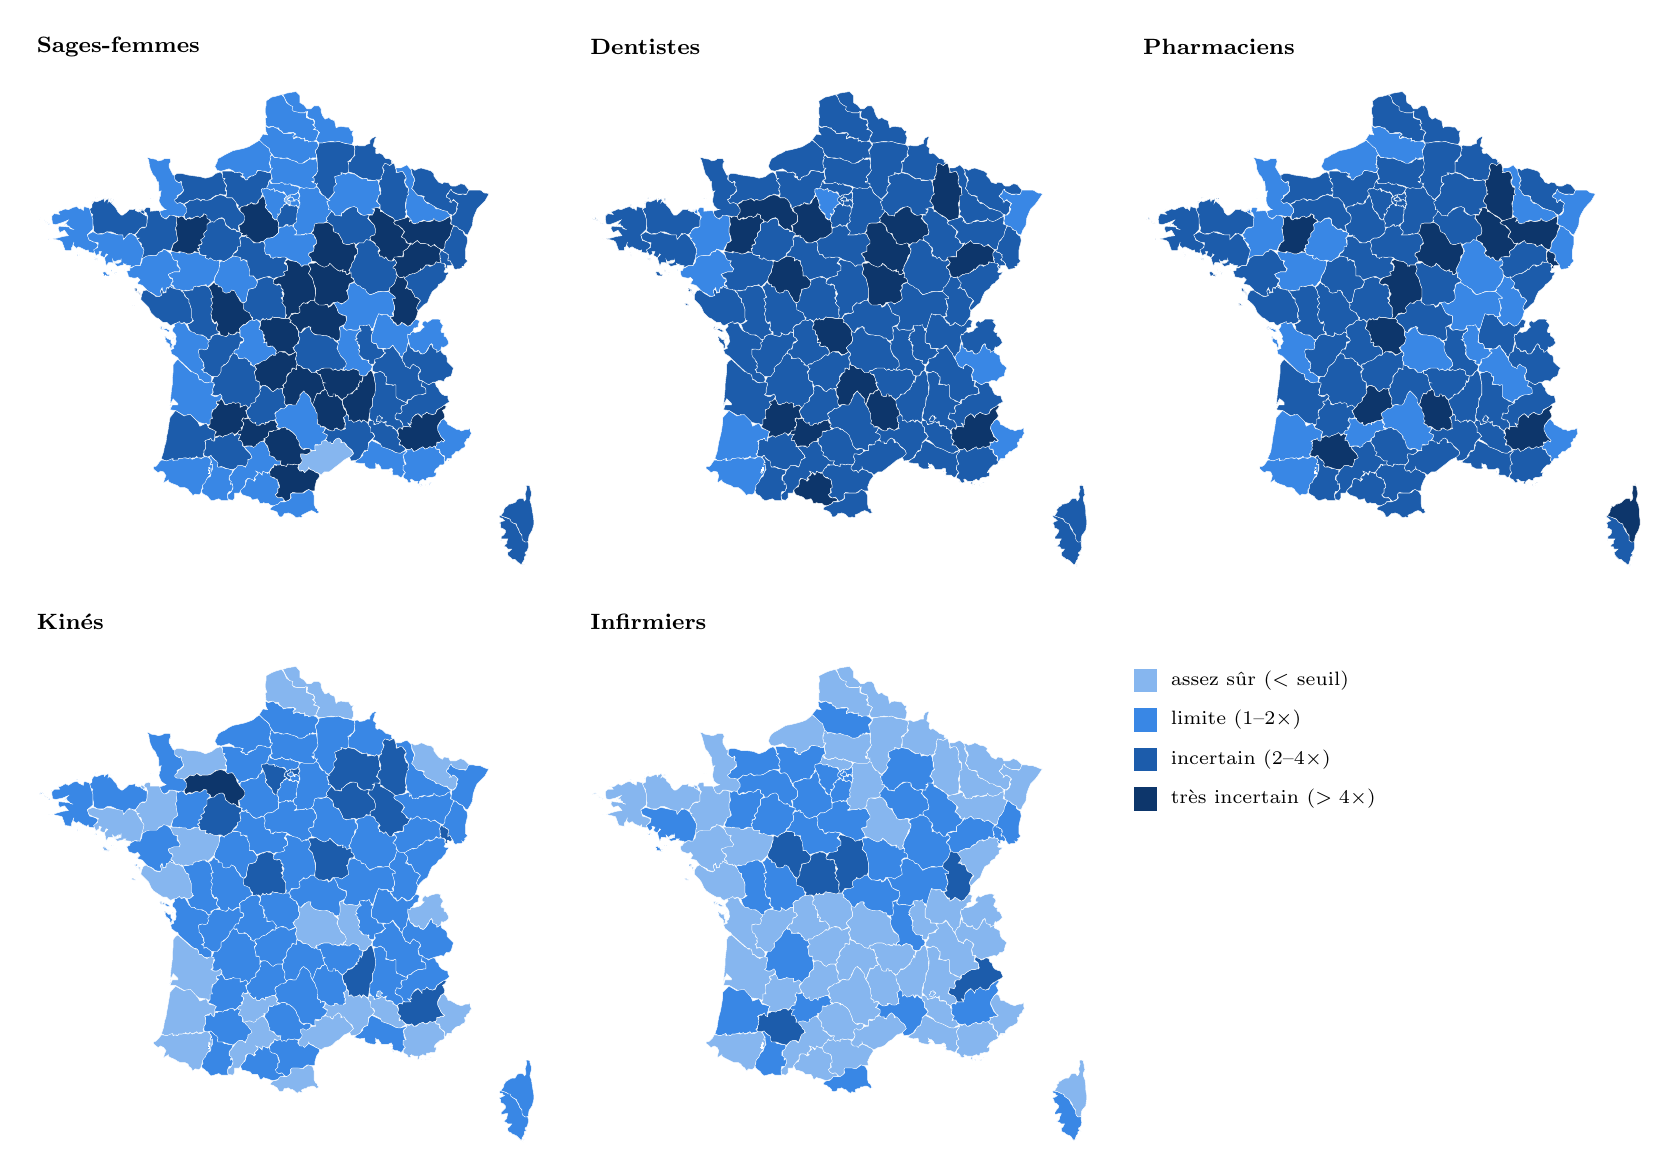
\begin{tikzpicture}[x=1cm,y=-1cm,line width=0.15pt]
\definecolor{cl0}{HTML}{86b6ef}
\definecolor{cl1}{HTML}{3987e5}
\definecolor{cl2}{HTML}{1c5cab}
\definecolor{cl3}{HTML}{0d366b}
\definecolor{clna}{HTML}{E4E3DF}
\node[anchor=west,font=\footnotesize\bfseries] at (0.00,-0.30) {Sages-femmes};
\fill[cl1,draw=white] (4.39,3.30) -- (4.41,3.24) -- (4.43,3.17) -- (4.44,3.11) -- (4.46,3.09) -- (4.47,3.09) -- (4.50,3.11) -- (4.52,3.10) -- (4.55,3.10) -- (4.57,3.10) -- (4.58,3.12) -- (4.61,3.13) -- (4.61,3.15) -- (4.62,3.16) -- (4.64,3.18) -- (4.65,3.21) -- (4.67,3.21) -- (4.68,3.23) -- (4.70,3.24) -- (4.73,3.23) -- (4.76,3.20) -- (4.78,3.22) -- (4.81,3.24) -- (4.86,3.24) -- (4.89,3.21) -- (4.90,3.18) -- (4.93,3.16) -- (4.98,3.18) -- (4.97,3.21) -- (4.96,3.23) -- (4.96,3.26) -- (4.93,3.27) -- (4.91,3.27) -- (4.90,3.30) -- (4.88,3.33) -- (4.86,3.36) -- (4.83,3.35) -- (4.83,3.39) -- (4.84,3.44) -- (4.82,3.52) -- (4.81,3.57) -- (4.78,3.59) -- (4.77,3.63) -- (4.74,3.64) -- (4.72,3.61) -- (4.73,3.60) -- (4.70,3.57) -- (4.66,3.52) -- (4.64,3.49) -- (4.61,3.52) -- (4.57,3.55) -- (4.54,3.53) -- (4.50,3.53) -- (4.46,3.53) -- (4.45,3.51) -- (4.43,3.47) -- (4.40,3.47) -- (4.37,3.45) -- (4.37,3.40) -- (4.37,3.35) -- (4.39,3.31) -- cycle;
\fill[cl2,draw=white] (3.70,0.92) -- (3.75,0.92) -- (3.79,0.91) -- (3.84,0.91) -- (3.89,0.91) -- (3.91,0.90) -- (3.96,0.90) -- (4.01,0.92) -- (4.05,0.93) -- (4.11,0.94) -- (4.15,0.96) -- (4.16,1.01) -- (4.15,1.07) -- (4.14,1.10) -- (4.11,1.13) -- (4.07,1.16) -- (4.08,1.19) -- (4.09,1.22) -- (4.08,1.27) -- (4.07,1.30) -- (4.03,1.31) -- (3.98,1.30) -- (3.99,1.33) -- (3.92,1.35) -- (3.91,1.39) -- (3.91,1.42) -- (3.93,1.44) -- (3.92,1.45) -- (3.90,1.50) -- (3.91,1.53) -- (3.88,1.57) -- (3.85,1.61) -- (3.82,1.64) -- (3.79,1.62) -- (3.76,1.60) -- (3.73,1.56) -- (3.71,1.52) -- (3.68,1.48) -- (3.67,1.46) -- (3.68,1.44) -- (3.67,1.45) -- (3.65,1.43) -- (3.63,1.43) -- (3.63,1.44) -- (3.61,1.42) -- (3.64,1.41) -- (3.64,1.39) -- (3.62,1.37) -- (3.61,1.35) -- (3.66,1.33) -- (3.68,1.28) -- (3.68,1.25) -- (3.68,1.21) -- (3.68,1.17) -- (3.68,1.13) -- (3.67,1.08) -- (3.66,1.05) -- (3.66,1.02) -- (3.68,0.99) -- (3.70,0.95) -- (3.70,0.93) -- cycle;
\fill[cl3,draw=white] (3.64,2.92) -- (3.69,2.97) -- (3.73,2.98) -- (3.77,2.98) -- (3.81,2.97) -- (3.82,3.01) -- (3.86,2.99) -- (3.88,2.96) -- (3.90,2.96) -- (3.93,3.00) -- (3.94,3.05) -- (3.97,3.09) -- (4.00,3.11) -- (4.04,3.11) -- (4.05,3.16) -- (4.06,3.21) -- (4.02,3.23) -- (3.98,3.25) -- (3.96,3.28) -- (3.97,3.31) -- (3.98,3.36) -- (3.98,3.40) -- (3.96,3.42) -- (3.93,3.44) -- (3.90,3.42) -- (3.87,3.40) -- (3.85,3.40) -- (3.83,3.38) -- (3.80,3.37) -- (3.76,3.37) -- (3.72,3.37) -- (3.68,3.36) -- (3.65,3.35) -- (3.61,3.33) -- (3.59,3.30) -- (3.60,3.27) -- (3.57,3.25) -- (3.55,3.27) -- (3.52,3.27) -- (3.49,3.30) -- (3.47,3.34) -- (3.44,3.31) -- (3.43,3.28) -- (3.41,3.25) -- (3.38,3.23) -- (3.36,3.21) -- (3.33,3.20) -- (3.34,3.18) -- (3.32,3.15) -- (3.34,3.11) -- (3.39,3.09) -- (3.43,3.09) -- (3.46,3.07) -- (3.45,3.04) -- (3.44,3.00) -- (3.47,2.99) -- (3.49,2.96) -- (3.52,2.95) -- (3.56,2.96) -- (3.59,2.92) -- (3.64,2.92) -- cycle;
\fill[cl3,draw=white] (4.77,4.53) -- (4.81,4.52) -- (4.86,4.52) -- (4.84,4.47) -- (4.88,4.48) -- (4.86,4.45) -- (4.89,4.40) -- (4.94,4.37) -- (4.96,4.36) -- (4.99,4.39) -- (5.01,4.41) -- (5.01,4.38) -- (5.04,4.36) -- (5.07,4.34) -- (5.10,4.36) -- (5.14,4.37) -- (5.18,4.36) -- (5.20,4.32) -- (5.23,4.29) -- (5.26,4.27) -- (5.29,4.25) -- (5.32,4.27) -- (5.30,4.30) -- (5.27,4.32) -- (5.29,4.36) -- (5.30,4.39) -- (5.29,4.42) -- (5.25,4.45) -- (5.23,4.48) -- (5.21,4.51) -- (5.21,4.55) -- (5.23,4.59) -- (5.25,4.65) -- (5.27,4.67) -- (5.30,4.71) -- (5.27,4.71) -- (5.24,4.72) -- (5.20,4.72) -- (5.20,4.76) -- (5.18,4.78) -- (5.14,4.79) -- (5.11,4.78) -- (5.08,4.80) -- (5.05,4.81) -- (5.03,4.79) -- (4.98,4.80) -- (4.94,4.83) -- (4.91,4.84) -- (4.88,4.81) -- (4.85,4.82) -- (4.81,4.81) -- (4.78,4.78) -- (4.74,4.76) -- (4.72,4.74) -- (4.73,4.70) -- (4.70,4.67) -- (4.71,4.61) -- (4.70,4.57) -- (4.73,4.53) -- (4.76,4.56) -- (4.77,4.53) -- cycle;
\fill[cl2,draw=white] (5.02,3.95) -- (5.06,3.96) -- (5.09,3.99) -- (5.11,3.98) -- (5.15,3.96) -- (5.18,3.97) -- (5.19,4.01) -- (5.22,4.04) -- (5.23,4.07) -- (5.26,4.11) -- (5.30,4.13) -- (5.34,4.13) -- (5.34,4.17) -- (5.36,4.21) -- (5.34,4.22) -- (5.31,4.24) -- (5.27,4.27) -- (5.24,4.29) -- (5.20,4.31) -- (5.18,4.36) -- (5.15,4.37) -- (5.10,4.36) -- (5.07,4.34) -- (5.05,4.36) -- (5.01,4.38) -- (5.01,4.41) -- (4.99,4.38) -- (4.96,4.36) -- (4.93,4.37) -- (4.89,4.41) -- (4.87,4.46) -- (4.87,4.50) -- (4.83,4.48) -- (4.87,4.53) -- (4.80,4.52) -- (4.77,4.52) -- (4.76,4.48) -- (4.74,4.45) -- (4.72,4.44) -- (4.68,4.43) -- (4.66,4.39) -- (4.68,4.37) -- (4.68,4.34) -- (4.74,4.36) -- (4.75,4.32) -- (4.75,4.28) -- (4.76,4.25) -- (4.80,4.24) -- (4.83,4.23) -- (4.83,4.19) -- (4.87,4.18) -- (4.89,4.16) -- (4.92,4.13) -- (4.96,4.12) -- (5.00,4.12) -- (5.04,4.11) -- (5.06,4.10) -- (5.05,4.06) -- (5.04,4.03) -- (5.00,4.00) -- (5.01,3.96) -- cycle;
\fill[cl1,draw=white] (5.36,4.95) -- (5.36,4.95) -- (5.36,4.95) -- (5.36,4.95) -- (5.36,4.95) -- (5.36,4.95) -- (5.36,4.95) -- (5.35,4.95) -- (5.35,4.95) -- (5.35,4.95) -- (5.35,4.95) -- (5.35,4.95) -- (5.35,4.95) -- (5.35,4.95) -- (5.35,4.95) -- (5.35,4.95) -- (5.36,4.95) -- (5.36,4.95) -- (5.36,4.95) -- (5.36,4.95) -- (5.36,4.95) -- (5.36,4.95) -- (5.36,4.95) -- (5.36,4.95) -- (5.36,4.95) -- (5.36,4.95) -- (5.36,4.95) -- cycle;
\fill[cl1,draw=white] (5.36,4.96) -- (5.35,4.96) -- (5.35,4.96) -- (5.35,4.96) -- (5.35,4.96) -- (5.35,4.95) -- (5.35,4.95) -- (5.35,4.95) -- (5.36,4.95) -- (5.36,4.95) -- (5.36,4.96) -- (5.36,4.96) -- (5.36,4.96) -- (5.36,4.96) -- (5.36,4.96) -- cycle;
\fill[cl1,draw=white] (5.29,4.43) -- (5.31,4.45) -- (5.33,4.47) -- (5.34,4.50) -- (5.37,4.51) -- (5.40,4.53) -- (5.42,4.54) -- (5.45,4.56) -- (5.48,4.56) -- (5.51,4.58) -- (5.54,4.57) -- (5.56,4.56) -- (5.60,4.56) -- (5.62,4.54) -- (5.62,4.58) -- (5.64,4.61) -- (5.62,4.64) -- (5.61,4.67) -- (5.58,4.68) -- (5.57,4.71) -- (5.55,4.73) -- (5.56,4.77) -- (5.55,4.79) -- (5.52,4.80) -- (5.50,4.82) -- (5.48,4.84) -- (5.47,4.85) -- (5.47,4.84) -- (5.44,4.84) -- (5.42,4.87) -- (5.39,4.89) -- (5.39,4.92) -- (5.39,4.93) -- (5.36,4.93) -- (5.33,4.93) -- (5.32,4.96) -- (5.30,4.97) -- (5.29,4.95) -- (5.30,4.91) -- (5.29,4.89) -- (5.27,4.89) -- (5.24,4.87) -- (5.24,4.84) -- (5.23,4.81) -- (5.19,4.81) -- (5.18,4.78) -- (5.20,4.76) -- (5.20,4.73) -- (5.23,4.73) -- (5.26,4.70) -- (5.28,4.72) -- (5.30,4.70) -- (5.27,4.67) -- (5.25,4.65) -- (5.23,4.61) -- (5.21,4.57) -- (5.21,4.54) -- (5.22,4.50) -- (5.24,4.48) -- (5.25,4.45) -- (5.28,4.43) -- cycle;
\fill[cl2,draw=white] (6.01,5.97) -- (6.01,5.97) -- (6.01,5.97) -- (6.01,5.97) -- (6.02,5.96) -- (6.02,5.96) -- (6.02,5.96) -- (6.02,5.97) -- (6.01,5.97) -- (6.02,5.97) -- (6.01,5.97) -- (6.01,5.97) -- (6.01,5.97) -- cycle;
\fill[cl2,draw=white] (6.35,6.16) -- (6.35,6.16) -- (6.35,6.16) -- (6.35,6.16) -- (6.35,6.16) -- (6.35,6.16) -- (6.35,6.16) -- (6.35,6.16) -- cycle;
\fill[cl2,draw=white] (5.99,5.66) -- (5.99,5.66) -- (5.99,5.66) -- (5.99,5.66) -- (5.99,5.66) -- (5.99,5.66) -- (5.99,5.66) -- (5.99,5.66) -- cycle;
\fill[cl2,draw=white] (6.30,6.30) -- (6.30,6.30) -- (6.30,6.30) -- (6.30,6.30) -- (6.30,6.30) -- (6.30,6.30) -- (6.30,6.30) -- (6.30,6.30) -- (6.30,6.30) -- (6.30,6.30) -- (6.29,6.30) -- (6.29,6.30) -- (6.29,6.30) -- (6.30,6.30) -- (6.30,6.30) -- (6.30,6.30) -- (6.30,6.29) -- (6.30,6.29) -- (6.30,6.30) -- (6.30,6.30) -- (6.30,6.30) -- (6.30,6.30) -- (6.30,6.30) -- (6.30,6.30) -- (6.30,6.30) -- cycle;
\fill[cl2,draw=white] (6.34,6.17) -- (6.34,6.17) -- (6.34,6.17) -- (6.34,6.17) -- (6.34,6.17) -- (6.34,6.17) -- (6.34,6.17) -- (6.34,6.17) -- (6.34,6.17) -- (6.34,6.17) -- cycle;
\fill[cl2,draw=white] (6.30,6.28) -- (6.30,6.28) -- (6.30,6.28) -- (6.30,6.28) -- (6.30,6.29) -- (6.30,6.28) -- (6.30,6.28) -- (6.30,6.28) -- (6.30,6.28) -- (6.30,6.28) -- (6.30,6.28) -- (6.30,6.28) -- (6.30,6.28) -- (6.30,6.28) -- (6.30,6.28) -- (6.30,6.28) -- (6.30,6.28) -- (6.30,6.28) -- (6.30,6.28) -- (6.30,6.28) -- (6.30,6.28) -- (6.30,6.28) -- (6.30,6.28) -- (6.30,6.28) -- (6.30,6.28) -- (6.30,6.28) -- (6.30,6.28) -- (6.30,6.28) -- (6.30,6.28) -- (6.31,6.28) -- (6.31,6.28) -- (6.30,6.28) -- (6.30,6.28) -- (6.30,6.28) -- cycle;
\fill[cl2,draw=white] (6.28,6.28) -- (6.29,6.28) -- (6.29,6.28) -- (6.29,6.28) -- (6.29,6.28) -- (6.28,6.28) -- cycle;
\fill[cl2,draw=white] (6.34,6.18) -- (6.34,6.18) -- (6.34,6.17) -- (6.34,6.17) -- (6.34,6.17) -- (6.34,6.18) -- cycle;
\fill[cl2,draw=white] (6.36,6.10) -- (6.35,6.10) -- (6.35,6.09) -- (6.36,6.09) -- (6.36,6.09) -- (6.36,6.09) -- (6.36,6.09) -- (6.36,6.10) -- (6.36,6.09) -- (6.36,6.10) -- cycle;
\fill[cl2,draw=white] (6.34,6.12) -- (6.34,6.12) -- (6.34,6.12) -- (6.34,6.12) -- (6.34,6.12) -- cycle;
\fill[cl2,draw=white] (6.01,5.65) -- (6.05,5.67) -- (6.10,5.69) -- (6.13,5.70) -- (6.16,5.74) -- (6.20,5.76) -- (6.23,5.82) -- (6.25,5.86) -- (6.28,5.91) -- (6.29,5.95) -- (6.32,5.99) -- (6.35,5.97) -- (6.36,6.01) -- (6.36,6.06) -- (6.35,6.09) -- (6.34,6.11) -- (6.32,6.12) -- (6.32,6.14) -- (6.34,6.15) -- (6.31,6.18) -- (6.31,6.21) -- (6.30,6.23) -- (6.28,6.26) -- (6.29,6.26) -- (6.27,6.28) -- (6.25,6.26) -- (6.23,6.25) -- (6.22,6.24) -- (6.21,6.23) -- (6.19,6.21) -- (6.16,6.21) -- (6.14,6.19) -- (6.11,6.17) -- (6.10,6.15) -- (6.10,6.12) -- (6.12,6.11) -- (6.15,6.08) -- (6.10,6.08) -- (6.08,6.05) -- (6.05,6.05) -- (6.07,6.02) -- (6.09,6.01) -- (6.09,5.98) -- (6.10,5.95) -- (6.07,5.95) -- (6.02,5.95) -- (6.02,5.92) -- (6.05,5.90) -- (6.07,5.87) -- (6.07,5.84) -- (6.04,5.82) -- (6.01,5.81) -- (6.01,5.78) -- (6.01,5.76) -- (5.99,5.75) -- (6.02,5.73) -- (6.06,5.72) -- (6.04,5.70) -- (6.03,5.69) -- (6.00,5.68) -- (5.99,5.66) -- cycle;
\fill[cl2,draw=white] (6.36,5.26) -- (6.36,5.26) -- (6.36,5.25) -- (6.36,5.25) -- (6.36,5.25) -- (6.36,5.25) -- (6.36,5.25) -- (6.36,5.26) -- (6.36,5.26) -- cycle;
\fill[cl2,draw=white] (6.33,5.29) -- (6.33,5.29) -- (6.33,5.29) -- (6.33,5.29) -- (6.33,5.29) -- cycle;
\fill[cl2,draw=white] (6.36,5.98) -- (6.34,5.99) -- (6.32,5.99) -- (6.29,5.97) -- (6.28,5.94) -- (6.28,5.90) -- (6.25,5.87) -- (6.24,5.83) -- (6.22,5.80) -- (6.21,5.76) -- (6.17,5.75) -- (6.14,5.73) -- (6.13,5.70) -- (6.11,5.69) -- (6.08,5.68) -- (6.05,5.67) -- (6.02,5.66) -- (6.02,5.65) -- (6.03,5.63) -- (6.04,5.62) -- (6.05,5.60) -- (6.05,5.58) -- (6.06,5.56) -- (6.07,5.55) -- (6.07,5.53) -- (6.08,5.54) -- (6.10,5.53) -- (6.11,5.51) -- (6.13,5.51) -- (6.15,5.50) -- (6.16,5.50) -- (6.19,5.49) -- (6.21,5.47) -- (6.22,5.45) -- (6.25,5.44) -- (6.28,5.44) -- (6.30,5.44) -- (6.31,5.47) -- (6.33,5.45) -- (6.33,5.42) -- (6.32,5.38) -- (6.33,5.35) -- (6.34,5.32) -- (6.34,5.30) -- (6.33,5.27) -- (6.36,5.27) -- (6.38,5.28) -- (6.38,5.30) -- (6.39,5.33) -- (6.40,5.36) -- (6.40,5.39) -- (6.39,5.42) -- (6.38,5.46) -- (6.40,5.52) -- (6.41,5.58) -- (6.42,5.64) -- (6.43,5.71) -- (6.43,5.77) -- (6.41,5.84) -- (6.37,5.91) -- (6.36,5.97) -- cycle;
\fill[cl3,draw=white] (4.26,3.88) -- (4.29,3.88) -- (4.31,3.87) -- (4.32,3.85) -- (4.33,3.82) -- (4.36,3.81) -- (4.38,3.83) -- (4.40,3.89) -- (4.41,3.94) -- (4.42,3.99) -- (4.42,4.04) -- (4.42,4.10) -- (4.40,4.14) -- (4.38,4.17) -- (4.39,4.23) -- (4.37,4.28) -- (4.35,4.30) -- (4.35,4.34) -- (4.34,4.39) -- (4.33,4.46) -- (4.31,4.47) -- (4.28,4.45) -- (4.26,4.44) -- (4.24,4.47) -- (4.22,4.44) -- (4.19,4.45) -- (4.16,4.49) -- (4.13,4.46) -- (4.11,4.44) -- (4.08,4.45) -- (4.07,4.44) -- (4.08,4.41) -- (4.08,4.39) -- (4.07,4.37) -- (4.05,4.36) -- (4.05,4.33) -- (4.04,4.30) -- (4.02,4.28) -- (4.01,4.25) -- (4.00,4.23) -- (4.00,4.21) -- (4.00,4.18) -- (4.02,4.17) -- (4.03,4.15) -- (4.05,4.14) -- (4.06,4.13) -- (4.06,4.12) -- (4.08,4.11) -- (4.12,4.11) -- (4.15,4.07) -- (4.16,4.06) -- (4.19,4.05) -- (4.18,4.02) -- (4.21,4.01) -- (4.21,3.99) -- (4.21,3.97) -- (4.22,3.96) -- (4.22,3.94) -- (4.24,3.96) -- (4.25,3.95) -- (4.26,3.92) -- cycle;
\fill[cl2,draw=white] (4.15,0.96) -- (4.19,0.95) -- (4.22,0.96) -- (4.28,0.96) -- (4.31,0.94) -- (4.35,0.93) -- (4.35,0.89) -- (4.38,0.86) -- (4.42,0.84) -- (4.43,0.85) -- (4.41,0.87) -- (4.41,0.89) -- (4.40,0.92) -- (4.39,0.96) -- (4.43,0.99) -- (4.42,1.01) -- (4.42,1.05) -- (4.44,1.06) -- (4.47,1.05) -- (4.51,1.07) -- (4.53,1.10) -- (4.55,1.12) -- (4.59,1.12) -- (4.62,1.14) -- (4.62,1.17) -- (4.64,1.16) -- (4.63,1.18) -- (4.60,1.21) -- (4.58,1.20) -- (4.55,1.19) -- (4.53,1.20) -- (4.52,1.22) -- (4.51,1.24) -- (4.52,1.27) -- (4.52,1.30) -- (4.52,1.32) -- (4.50,1.35) -- (4.50,1.37) -- (4.48,1.39) -- (4.45,1.39) -- (4.43,1.39) -- (4.41,1.41) -- (4.39,1.40) -- (4.35,1.39) -- (4.32,1.39) -- (4.31,1.37) -- (4.27,1.38) -- (4.21,1.35) -- (4.18,1.33) -- (4.15,1.31) -- (4.08,1.29) -- (4.08,1.27) -- (4.08,1.23) -- (4.08,1.21) -- (4.08,1.19) -- (4.07,1.16) -- (4.10,1.16) -- (4.12,1.12) -- (4.14,1.10) -- (4.16,1.08) -- (4.15,1.05) -- (4.16,0.99) -- (4.15,0.96) -- cycle;
\fill[cl1,draw=white] (3.07,5.10) -- (3.08,5.13) -- (3.10,5.16) -- (3.13,5.18) -- (3.14,5.18) -- (3.16,5.19) -- (3.18,5.21) -- (3.18,5.24) -- (3.19,5.27) -- (3.20,5.30) -- (3.18,5.31) -- (3.18,5.36) -- (3.15,5.39) -- (3.17,5.42) -- (3.21,5.43) -- (3.24,5.43) -- (3.26,5.45) -- (3.25,5.47) -- (3.21,5.48) -- (3.19,5.51) -- (3.16,5.52) -- (3.12,5.53) -- (3.08,5.52) -- (3.06,5.50) -- (3.02,5.50) -- (3.00,5.49) -- (2.98,5.50) -- (2.95,5.50) -- (2.94,5.47) -- (2.92,5.44) -- (2.88,5.45) -- (2.85,5.45) -- (2.83,5.42) -- (2.79,5.41) -- (2.76,5.40) -- (2.73,5.39) -- (2.71,5.36) -- (2.70,5.32) -- (2.72,5.30) -- (2.76,5.29) -- (2.77,5.25) -- (2.78,5.22) -- (2.78,5.20) -- (2.80,5.19) -- (2.82,5.18) -- (2.85,5.18) -- (2.88,5.22) -- (2.90,5.19) -- (2.88,5.18) -- (2.88,5.15) -- (2.91,5.15) -- (2.93,5.12) -- (2.91,5.11) -- (2.91,5.09) -- (2.94,5.09) -- (2.96,5.12) -- (2.98,5.14) -- (2.98,5.11) -- (2.99,5.09) -- (3.02,5.10) -- (3.05,5.12) -- cycle;
\fill[cl2,draw=white] (3.80,1.93) -- (3.80,1.91) -- (3.80,1.88) -- (3.80,1.87) -- (3.81,1.84) -- (3.83,1.82) -- (3.86,1.79) -- (3.89,1.81) -- (3.90,1.84) -- (3.93,1.84) -- (3.96,1.84) -- (3.99,1.85) -- (3.99,1.81) -- (4.01,1.81) -- (4.04,1.78) -- (4.07,1.76) -- (4.12,1.73) -- (4.16,1.73) -- (4.19,1.74) -- (4.19,1.79) -- (4.23,1.83) -- (4.28,1.84) -- (4.29,1.83) -- (4.33,1.83) -- (4.34,1.85) -- (4.32,1.88) -- (4.34,1.90) -- (4.37,1.93) -- (4.39,1.95) -- (4.41,1.96) -- (4.41,1.99) -- (4.42,2.02) -- (4.42,2.05) -- (4.42,2.08) -- (4.38,2.10) -- (4.35,2.12) -- (4.36,2.13) -- (4.34,2.16) -- (4.30,2.15) -- (4.29,2.19) -- (4.24,2.20) -- (4.21,2.19) -- (4.18,2.21) -- (4.15,2.20) -- (4.14,2.20) -- (4.12,2.20) -- (4.09,2.21) -- (4.07,2.21) -- (4.04,2.21) -- (4.01,2.20) -- (4.00,2.17) -- (3.99,2.17) -- (3.99,2.16) -- (3.98,2.13) -- (3.96,2.10) -- (3.95,2.07) -- (3.92,2.07) -- (3.88,2.06) -- (3.89,2.03) -- (3.88,2.00) -- (3.87,1.97) -- (3.83,1.94) -- cycle;
\fill[cl3,draw=white] (3.07,5.10) -- (3.09,5.08) -- (3.10,5.05) -- (3.12,5.05) -- (3.13,5.03) -- (3.13,5.00) -- (3.16,5.02) -- (3.17,5.01) -- (3.19,5.01) -- (3.22,5.00) -- (3.23,5.02) -- (3.26,5.02) -- (3.29,5.03) -- (3.30,5.01) -- (3.32,4.99) -- (3.36,5.01) -- (3.39,5.00) -- (3.42,5.00) -- (3.45,5.02) -- (3.43,5.05) -- (3.46,5.08) -- (3.48,5.09) -- (3.50,5.08) -- (3.51,5.10) -- (3.55,5.08) -- (3.57,5.06) -- (3.57,5.04) -- (3.59,5.07) -- (3.63,5.08) -- (3.67,5.11) -- (3.70,5.12) -- (3.71,5.16) -- (3.67,5.21) -- (3.65,5.29) -- (3.65,5.34) -- (3.59,5.34) -- (3.55,5.33) -- (3.49,5.37) -- (3.43,5.37) -- (3.37,5.36) -- (3.34,5.39) -- (3.34,5.44) -- (3.30,5.47) -- (3.27,5.47) -- (3.25,5.44) -- (3.23,5.42) -- (3.19,5.43) -- (3.16,5.41) -- (3.15,5.39) -- (3.18,5.36) -- (3.18,5.31) -- (3.20,5.30) -- (3.20,5.27) -- (3.19,5.24) -- (3.18,5.22) -- (3.17,5.19) -- (3.15,5.19) -- (3.13,5.17) -- (3.11,5.17) -- (3.08,5.15) -- (3.08,5.12) -- cycle;
\fill[cl1,draw=white] (3.29,4.27) -- (3.32,4.24) -- (3.36,4.25) -- (3.40,4.25) -- (3.42,4.21) -- (3.44,4.20) -- (3.45,4.16) -- (3.46,4.13) -- (3.48,4.10) -- (3.51,4.07) -- (3.53,4.09) -- (3.55,4.11) -- (3.57,4.13) -- (3.60,4.17) -- (3.60,4.21) -- (3.62,4.25) -- (3.66,4.31) -- (3.68,4.36) -- (3.68,4.41) -- (3.69,4.45) -- (3.68,4.49) -- (3.72,4.50) -- (3.74,4.53) -- (3.78,4.53) -- (3.77,4.58) -- (3.75,4.60) -- (3.78,4.61) -- (3.82,4.64) -- (3.78,4.69) -- (3.75,4.72) -- (3.73,4.76) -- (3.66,4.75) -- (3.66,4.79) -- (3.65,4.83) -- (3.62,4.83) -- (3.59,4.81) -- (3.54,4.80) -- (3.49,4.81) -- (3.46,4.77) -- (3.44,4.72) -- (3.42,4.69) -- (3.41,4.65) -- (3.39,4.62) -- (3.36,4.59) -- (3.33,4.57) -- (3.28,4.56) -- (3.30,4.55) -- (3.27,4.54) -- (3.24,4.54) -- (3.22,4.55) -- (3.19,4.54) -- (3.16,4.53) -- (3.18,4.50) -- (3.17,4.48) -- (3.15,4.44) -- (3.15,4.41) -- (3.14,4.37) -- (3.16,4.34) -- (3.20,4.31) -- (3.23,4.29) -- (3.28,4.28) -- cycle;
\fill[cl1,draw=white] (4.65,5.16) -- (4.65,5.16) -- (4.65,5.16) -- (4.65,5.16) -- (4.65,5.16) -- (4.64,5.16) -- (4.64,5.16) -- (4.64,5.16) -- (4.64,5.16) -- (4.64,5.16) -- (4.64,5.16) -- (4.64,5.16) -- (4.64,5.16) -- (4.64,5.16) -- (4.64,5.16) -- (4.65,5.16) -- (4.65,5.16) -- (4.65,5.16) -- (4.65,5.16) -- (4.65,5.16) -- cycle;
\fill[cl1,draw=white] (4.65,5.16) -- (4.64,5.15) -- (4.64,5.15) -- (4.64,5.15) -- (4.65,5.15) -- (4.65,5.15) -- (4.65,5.15) -- (4.65,5.15) -- (4.65,5.16) -- cycle;
\fill[cl1,draw=white] (4.75,5.17) -- (4.74,5.17) -- (4.74,5.17) -- (4.74,5.17) -- (4.75,5.17) -- (4.75,5.17) -- (4.75,5.17) -- (4.75,5.17) -- cycle;
\fill[cl1,draw=white] (4.61,5.10) -- (4.61,5.10) -- (4.61,5.10) -- (4.61,5.10) -- (4.61,5.10) -- (4.61,5.10) -- (4.61,5.10) -- (4.61,5.10) -- (4.61,5.10) -- (4.61,5.10) -- (4.61,5.11) -- (4.61,5.11) -- (4.61,5.11) -- (4.60,5.11) -- (4.60,5.11) -- (4.60,5.11) -- (4.60,5.11) -- (4.60,5.10) -- (4.61,5.10) -- (4.61,5.10) -- (4.61,5.10) -- (4.61,5.10) -- (4.61,5.10) -- (4.61,5.10) -- (4.61,5.10) -- (4.61,5.10) -- (4.61,5.10) -- (4.61,5.10) -- (4.61,5.10) -- (4.61,5.10) -- (4.61,5.10) -- (4.61,5.10) -- (4.61,5.10) -- (4.61,5.10) -- (4.61,5.10) -- (4.61,5.10) -- (4.61,5.09) -- (4.61,5.09) -- (4.61,5.09) -- (4.61,5.09) -- (4.61,5.09) -- (4.61,5.09) -- (4.61,5.09) -- (4.61,5.09) -- (4.61,5.09) -- (4.61,5.09) -- (4.62,5.09) -- (4.62,5.09) -- (4.62,5.09) -- (4.62,5.09) -- (4.62,5.09) -- (4.62,5.09) -- (4.62,5.09) -- (4.62,5.09) -- (4.62,5.10) -- (4.61,5.10) -- (4.61,5.10) -- (4.61,5.10) -- (4.61,5.10) -- (4.61,5.10) -- (4.61,5.10) -- cycle;
\fill[cl1,draw=white] (4.63,5.14) -- (4.62,5.14) -- (4.62,5.14) -- (4.62,5.14) -- (4.62,5.14) -- (4.62,5.14) -- (4.62,5.14) -- (4.62,5.14) -- (4.63,5.14) -- (4.63,5.14) -- (4.63,5.14) -- (4.63,5.14) -- (4.63,5.14) -- cycle;
\fill[cl1,draw=white] (4.64,5.15) -- (4.64,5.15) -- (4.64,5.15) -- (4.64,5.15) -- (4.64,5.15) -- (4.64,5.15) -- (4.64,5.15) -- (4.64,5.15) -- (4.64,5.15) -- cycle;
\fill[cl1,draw=white] (4.62,5.10) -- (4.62,5.10) -- (4.62,5.10) -- (4.62,5.10) -- (4.62,5.10) -- cycle;
\fill[cl1,draw=white] (4.62,5.06) -- (4.63,5.06) -- (4.63,5.07) -- (4.63,5.07) -- (4.63,5.07) -- (4.63,5.07) -- (4.63,5.08) -- (4.64,5.08) -- (4.63,5.08) -- (4.64,5.08) -- (4.63,5.07) -- (4.63,5.06) -- (4.62,5.06) -- (4.62,5.06) -- (4.62,5.05) -- (4.62,5.05) -- (4.62,5.06) -- (4.62,5.06) -- (4.62,5.06) -- cycle;
\fill[cl1,draw=white] (4.43,5.04) -- (4.43,5.05) -- (4.43,5.05) -- (4.43,5.04) -- (4.43,5.04) -- (4.43,5.04) -- (4.43,5.04) -- (4.43,5.04) -- (4.43,5.04) -- cycle;
\fill[cl1,draw=white] (4.37,4.70) -- (4.50,4.76) -- (4.60,4.81) -- (4.67,4.85) -- (4.74,4.86) -- (4.78,4.84) -- (4.82,4.83) -- (4.81,4.86) -- (4.78,4.88) -- (4.77,4.91) -- (4.78,4.93) -- (4.78,4.96) -- (4.79,4.99) -- (4.81,5.02) -- (4.78,5.04) -- (4.77,5.07) -- (4.81,5.10) -- (4.78,5.12) -- (4.76,5.16) -- (4.74,5.17) -- (4.72,5.16) -- (4.70,5.14) -- (4.69,5.14) -- (4.67,5.14) -- (4.65,5.14) -- (4.63,5.13) -- (4.64,5.11) -- (4.63,5.09) -- (4.64,5.07) -- (4.63,5.06) -- (4.62,5.05) -- (4.60,5.06) -- (4.58,5.07) -- (4.55,5.07) -- (4.52,5.07) -- (4.50,5.07) -- (4.49,5.06) -- (4.48,5.03) -- (4.47,5.02) -- (4.46,5.00) -- (4.44,5.01) -- (4.42,4.99) -- (4.42,5.02) -- (4.42,5.03) -- (4.42,5.04) -- (4.44,5.04) -- (4.41,5.06) -- (4.34,5.06) -- (4.29,5.03) -- (4.28,4.99) -- (4.22,4.99) -- (4.15,4.98) -- (4.19,4.94) -- (4.20,4.93) -- (4.23,4.92) -- (4.26,4.89) -- (4.26,4.85) -- (4.29,4.84) -- (4.32,4.82) -- (4.33,4.76) -- (4.33,4.74) -- (4.35,4.72) -- cycle;
\fill[cl2,draw=white] (2.16,1.63) -- (2.16,1.63) -- (2.16,1.63) -- (2.16,1.63) -- (2.16,1.63) -- cycle;
\fill[cl2,draw=white] (1.87,1.33) -- (1.90,1.31) -- (1.96,1.31) -- (2.04,1.33) -- (2.11,1.34) -- (2.19,1.35) -- (2.26,1.37) -- (2.34,1.35) -- (2.39,1.31) -- (2.45,1.29) -- (2.48,1.32) -- (2.48,1.36) -- (2.49,1.37) -- (2.50,1.39) -- (2.50,1.41) -- (2.51,1.44) -- (2.53,1.46) -- (2.52,1.49) -- (2.52,1.50) -- (2.51,1.53) -- (2.54,1.54) -- (2.52,1.58) -- (2.48,1.58) -- (2.45,1.57) -- (2.42,1.59) -- (2.39,1.59) -- (2.36,1.61) -- (2.32,1.64) -- (2.29,1.65) -- (2.27,1.66) -- (2.25,1.64) -- (2.22,1.64) -- (2.20,1.66) -- (2.19,1.64) -- (2.16,1.63) -- (2.14,1.64) -- (2.11,1.65) -- (2.07,1.65) -- (2.06,1.66) -- (2.01,1.68) -- (1.99,1.70) -- (1.97,1.69) -- (1.94,1.68) -- (1.90,1.69) -- (1.88,1.68) -- (1.86,1.66) -- (1.87,1.64) -- (1.90,1.62) -- (1.91,1.60) -- (1.92,1.59) -- (1.95,1.57) -- (1.98,1.53) -- (1.98,1.51) -- (1.96,1.49) -- (1.95,1.46) -- (1.95,1.45) -- (1.96,1.42) -- (1.95,1.41) -- (1.92,1.43) -- (1.90,1.41) -- (1.87,1.39) -- (1.87,1.38) -- cycle;
\fill[cl3,draw=white] (3.42,3.73) -- (3.44,3.75) -- (3.47,3.75) -- (3.49,3.78) -- (3.52,3.79) -- (3.56,3.79) -- (3.60,3.83) -- (3.65,3.84) -- (3.67,3.81) -- (3.67,3.84) -- (3.69,3.85) -- (3.71,3.86) -- (3.72,3.88) -- (3.74,3.90) -- (3.75,3.94) -- (3.78,3.96) -- (3.75,3.97) -- (3.76,3.99) -- (3.77,4.02) -- (3.78,4.05) -- (3.74,4.07) -- (3.72,4.09) -- (3.70,4.11) -- (3.68,4.10) -- (3.67,4.13) -- (3.65,4.17) -- (3.64,4.21) -- (3.62,4.25) -- (3.60,4.21) -- (3.60,4.17) -- (3.57,4.13) -- (3.55,4.11) -- (3.53,4.10) -- (3.51,4.07) -- (3.49,4.09) -- (3.46,4.12) -- (3.46,4.16) -- (3.44,4.19) -- (3.43,4.21) -- (3.41,4.25) -- (3.37,4.25) -- (3.34,4.24) -- (3.29,4.25) -- (3.27,4.25) -- (3.26,4.22) -- (3.26,4.18) -- (3.27,4.15) -- (3.24,4.11) -- (3.24,4.07) -- (3.24,4.04) -- (3.25,4.02) -- (3.25,3.99) -- (3.28,3.97) -- (3.29,3.94) -- (3.29,3.91) -- (3.30,3.88) -- (3.33,3.84) -- (3.36,3.80) -- (3.38,3.78) -- (3.42,3.80) -- (3.41,3.76) -- cycle;
\fill[cl2,draw=white] (2.30,3.43) -- (2.33,3.41) -- (2.35,3.37) -- (2.38,3.35) -- (2.41,3.35) -- (2.45,3.36) -- (2.49,3.37) -- (2.53,3.38) -- (2.55,3.36) -- (2.55,3.33) -- (2.58,3.35) -- (2.61,3.36) -- (2.64,3.35) -- (2.67,3.32) -- (2.69,3.33) -- (2.70,3.35) -- (2.70,3.38) -- (2.73,3.40) -- (2.75,3.42) -- (2.74,3.44) -- (2.70,3.45) -- (2.70,3.48) -- (2.69,3.52) -- (2.67,3.54) -- (2.65,3.55) -- (2.63,3.58) -- (2.61,3.60) -- (2.59,3.62) -- (2.57,3.63) -- (2.57,3.66) -- (2.55,3.70) -- (2.53,3.73) -- (2.49,3.74) -- (2.48,3.76) -- (2.46,3.79) -- (2.46,3.85) -- (2.43,3.87) -- (2.41,3.90) -- (2.37,3.89) -- (2.35,3.89) -- (2.30,3.87) -- (2.28,3.84) -- (2.24,3.84) -- (2.23,3.82) -- (2.23,3.80) -- (2.24,3.78) -- (2.24,3.76) -- (2.24,3.73) -- (2.23,3.70) -- (2.22,3.69) -- (2.19,3.66) -- (2.16,3.64) -- (2.17,3.59) -- (2.16,3.56) -- (2.19,3.54) -- (2.24,3.53) -- (2.27,3.54) -- (2.29,3.53) -- (2.29,3.49) -- (2.28,3.46) -- (2.30,3.43) -- cycle;
\fill[cl1,draw=white] (1.87,3.44) -- (1.87,3.44) -- (1.87,3.44) -- (1.87,3.44) -- (1.87,3.43) -- (1.87,3.43) -- (1.87,3.43) -- (1.87,3.43) -- (1.87,3.43) -- (1.87,3.44) -- (1.87,3.44) -- (1.88,3.44) -- (1.88,3.44) -- (1.87,3.44) -- (1.87,3.44) -- (1.87,3.44) -- (1.87,3.44) -- cycle;
\fill[cl1,draw=white] (1.72,3.28) -- (1.72,3.28) -- (1.72,3.28) -- (1.72,3.27) -- (1.72,3.27) -- (1.73,3.27) -- (1.74,3.27) -- (1.74,3.27) -- (1.74,3.27) -- (1.73,3.28) -- (1.73,3.28) -- (1.74,3.28) -- (1.74,3.28) -- (1.75,3.28) -- (1.76,3.28) -- (1.77,3.28) -- (1.78,3.29) -- (1.79,3.29) -- (1.79,3.29) -- (1.80,3.30) -- (1.80,3.30) -- (1.80,3.31) -- (1.81,3.31) -- (1.81,3.31) -- (1.80,3.32) -- (1.80,3.32) -- (1.79,3.32) -- (1.79,3.32) -- (1.78,3.32) -- (1.77,3.31) -- (1.77,3.31) -- (1.76,3.30) -- (1.75,3.30) -- (1.73,3.29) -- (1.72,3.28) -- (1.71,3.29) -- (1.70,3.29) -- (1.70,3.29) -- (1.69,3.28) -- (1.69,3.28) -- (1.69,3.27) -- (1.68,3.26) -- (1.68,3.26) -- (1.69,3.26) -- (1.70,3.25) -- (1.70,3.25) -- (1.71,3.25) -- (1.71,3.26) -- (1.72,3.26) -- (1.71,3.27) -- (1.71,3.27) -- (1.71,3.26) -- (1.71,3.27) -- (1.70,3.27) -- (1.70,3.27) -- (1.70,3.27) -- (1.71,3.28) -- (1.71,3.28) -- (1.71,3.28) -- (1.71,3.28) -- (1.71,3.28) -- (1.71,3.28) -- cycle;
\fill[cl1,draw=white] (1.85,3.41) -- (1.84,3.40) -- (1.84,3.40) -- (1.84,3.40) -- (1.84,3.40) -- (1.84,3.40) -- (1.84,3.40) -- (1.85,3.40) -- (1.85,3.40) -- (1.85,3.39) -- (1.85,3.40) -- (1.85,3.39) -- (1.85,3.40) -- (1.85,3.40) -- (1.85,3.40) -- (1.85,3.40) -- (1.85,3.40) -- (1.85,3.40) -- (1.85,3.40) -- (1.85,3.40) -- (1.85,3.40) -- (1.85,3.40) -- (1.85,3.40) -- (1.85,3.40) -- (1.85,3.40) -- (1.85,3.40) -- (1.85,3.40) -- (1.85,3.40) -- (1.85,3.41) -- cycle;
\fill[cl1,draw=white] (1.87,3.22) -- (1.89,3.21) -- (1.95,3.18) -- (1.95,3.22) -- (1.98,3.21) -- (2.00,3.21) -- (2.03,3.26) -- (2.05,3.30) -- (2.09,3.32) -- (2.11,3.32) -- (2.13,3.34) -- (2.17,3.34) -- (2.20,3.36) -- (2.26,3.38) -- (2.28,3.41) -- (2.31,3.44) -- (2.29,3.46) -- (2.30,3.50) -- (2.28,3.54) -- (2.25,3.55) -- (2.22,3.54) -- (2.18,3.54) -- (2.17,3.57) -- (2.18,3.61) -- (2.18,3.64) -- (2.21,3.67) -- (2.22,3.70) -- (2.24,3.72) -- (2.23,3.75) -- (2.25,3.78) -- (2.21,3.80) -- (2.24,3.82) -- (2.24,3.84) -- (2.27,3.84) -- (2.30,3.86) -- (2.34,3.89) -- (2.34,3.93) -- (2.33,3.97) -- (2.29,3.97) -- (2.24,3.96) -- (2.21,3.93) -- (2.18,3.92) -- (2.17,3.88) -- (2.14,3.85) -- (2.11,3.85) -- (2.09,3.83) -- (1.92,3.67) -- (1.91,3.65) -- (1.88,3.63) -- (1.83,3.60) -- (1.82,3.55) -- (1.86,3.53) -- (1.85,3.50) -- (1.88,3.48) -- (1.89,3.44) -- (1.88,3.41) -- (1.89,3.38) -- (1.87,3.34) -- (1.84,3.31) -- (1.84,3.29) -- (1.87,3.25) -- cycle;
\fill[cl1,draw=white] (1.81,3.51) -- (1.81,3.49) -- (1.81,3.48) -- (1.80,3.48) -- (1.80,3.47) -- (1.79,3.47) -- (1.79,3.47) -- (1.78,3.47) -- (1.78,3.46) -- (1.78,3.46) -- (1.77,3.46) -- (1.77,3.45) -- (1.76,3.45) -- (1.76,3.44) -- (1.76,3.44) -- (1.75,3.44) -- (1.76,3.43) -- (1.75,3.43) -- (1.75,3.42) -- (1.75,3.42) -- (1.75,3.41) -- (1.75,3.40) -- (1.75,3.40) -- (1.75,3.39) -- (1.74,3.38) -- (1.74,3.38) -- (1.75,3.38) -- (1.75,3.38) -- (1.76,3.38) -- (1.76,3.39) -- (1.76,3.39) -- (1.77,3.39) -- (1.77,3.40) -- (1.77,3.40) -- (1.78,3.40) -- (1.78,3.40) -- (1.78,3.41) -- (1.78,3.41) -- (1.79,3.41) -- (1.80,3.42) -- (1.80,3.42) -- (1.82,3.42) -- (1.82,3.42) -- (1.82,3.43) -- (1.82,3.43) -- (1.82,3.43) -- (1.82,3.43) -- (1.82,3.44) -- (1.82,3.44) -- (1.82,3.45) -- (1.82,3.45) -- (1.82,3.45) -- (1.82,3.46) -- (1.83,3.46) -- (1.83,3.47) -- (1.83,3.47) -- (1.84,3.48) -- (1.84,3.48) -- (1.84,3.48) -- (1.84,3.49) -- (1.84,3.49) -- (1.84,3.49) -- (1.84,3.49) -- (1.83,3.50) -- (1.83,3.50) -- (1.83,3.51) -- (1.83,3.51) -- (1.84,3.51) -- (1.83,3.52) -- (1.83,3.52) -- (1.83,3.53) -- (1.82,3.53) -- (1.82,3.53) -- (1.82,3.53) -- (1.82,3.53) -- (1.81,3.51) -- cycle;
\fill[cl3,draw=white] (3.30,2.40) -- (3.35,2.42) -- (3.39,2.42) -- (3.45,2.44) -- (3.47,2.47) -- (3.49,2.49) -- (3.51,2.47) -- (3.54,2.47) -- (3.57,2.47) -- (3.60,2.52) -- (3.57,2.58) -- (3.62,2.64) -- (3.64,2.71) -- (3.65,2.76) -- (3.66,2.82) -- (3.66,2.88) -- (3.64,2.92) -- (3.60,2.92) -- (3.57,2.94) -- (3.53,2.96) -- (3.51,2.95) -- (3.49,2.96) -- (3.47,2.99) -- (3.45,3.00) -- (3.45,3.02) -- (3.46,3.04) -- (3.46,3.07) -- (3.43,3.09) -- (3.40,3.08) -- (3.35,3.09) -- (3.34,3.12) -- (3.31,3.15) -- (3.27,3.15) -- (3.29,3.11) -- (3.28,3.09) -- (3.28,3.04) -- (3.28,3.01) -- (3.26,2.99) -- (3.24,2.97) -- (3.23,2.94) -- (3.24,2.92) -- (3.24,2.89) -- (3.26,2.84) -- (3.24,2.80) -- (3.24,2.78) -- (3.22,2.76) -- (3.22,2.73) -- (3.21,2.72) -- (3.19,2.71) -- (3.15,2.73) -- (3.11,2.71) -- (3.13,2.66) -- (3.16,2.64) -- (3.19,2.62) -- (3.25,2.61) -- (3.26,2.59) -- (3.24,2.56) -- (3.30,2.54) -- (3.30,2.49) -- (3.29,2.45) -- (3.26,2.43) -- (3.30,2.41) -- cycle;
\fill[cl3,draw=white] (3.16,3.60) -- (3.18,3.58) -- (3.20,3.56) -- (3.24,3.58) -- (3.28,3.58) -- (3.30,3.60) -- (3.32,3.62) -- (3.35,3.61) -- (3.38,3.59) -- (3.41,3.57) -- (3.42,3.60) -- (3.42,3.62) -- (3.41,3.64) -- (3.40,3.67) -- (3.42,3.69) -- (3.42,3.74) -- (3.41,3.77) -- (3.41,3.80) -- (3.38,3.78) -- (3.36,3.78) -- (3.35,3.83) -- (3.31,3.85) -- (3.29,3.89) -- (3.29,3.92) -- (3.29,3.94) -- (3.28,3.96) -- (3.26,3.98) -- (3.24,4.00) -- (3.26,4.03) -- (3.23,4.04) -- (3.20,4.05) -- (3.17,4.04) -- (3.15,4.06) -- (3.12,4.08) -- (3.09,4.07) -- (3.08,4.04) -- (3.05,4.02) -- (3.02,4.00) -- (2.99,4.01) -- (2.96,4.01) -- (2.94,3.97) -- (2.94,3.95) -- (2.90,3.94) -- (2.90,3.92) -- (2.89,3.88) -- (2.87,3.86) -- (2.89,3.82) -- (2.91,3.79) -- (2.89,3.78) -- (2.90,3.77) -- (2.88,3.75) -- (2.90,3.73) -- (2.93,3.73) -- (2.96,3.70) -- (2.98,3.68) -- (3.00,3.68) -- (3.03,3.67) -- (3.05,3.66) -- (3.08,3.63) -- (3.11,3.61) -- (3.13,3.62) -- (3.15,3.61) -- cycle;
\fill[cl2,draw=white] (4.10,2.71) -- (4.10,2.71) -- (4.10,2.71) -- (4.10,2.71) -- (4.10,2.71) -- (4.10,2.71) -- (4.10,2.71) -- (4.10,2.71) -- (4.10,2.71) -- (4.11,2.71) -- (4.11,2.70) -- (4.10,2.70) -- (4.10,2.70) -- (4.10,2.70) -- (4.10,2.70) -- (4.10,2.70) -- (4.11,2.70) -- (4.11,2.70) -- (4.11,2.70) -- (4.11,2.70) -- (4.11,2.70) -- (4.11,2.70) -- (4.11,2.70) -- (4.11,2.70) -- (4.11,2.70) -- (4.12,2.70) -- (4.12,2.70) -- (4.12,2.70) -- (4.12,2.70) -- (4.12,2.70) -- (4.13,2.70) -- (4.13,2.70) -- (4.13,2.70) -- (4.13,2.70) -- (4.13,2.70) -- (4.13,2.70) -- (4.13,2.70) -- (4.13,2.70) -- (4.13,2.70) -- (4.13,2.70) -- (4.14,2.70) -- (4.13,2.70) -- (4.13,2.70) -- (4.14,2.70) -- (4.13,2.70) -- (4.13,2.70) -- (4.13,2.71) -- (4.13,2.71) -- (4.13,2.71) -- (4.13,2.71) -- (4.13,2.71) -- (4.13,2.71) -- (4.13,2.71) -- (4.13,2.71) -- (4.13,2.71) -- (4.13,2.71) -- (4.13,2.71) -- (4.13,2.71) -- (4.13,2.71) -- (4.13,2.72) -- (4.13,2.72) -- (4.13,2.72) -- (4.13,2.72) -- (4.13,2.72) -- (4.13,2.72) -- (4.13,2.72) -- (4.13,2.72) -- (4.12,2.71) -- (4.12,2.71) -- (4.12,2.72) -- (4.12,2.72) -- (4.12,2.72) -- (4.12,2.72) -- (4.12,2.72) -- (4.12,2.72) -- (4.12,2.72) -- (4.11,2.72) -- (4.11,2.71) -- (4.11,2.71) -- (4.11,2.71) -- (4.11,2.71) -- (4.11,2.71) -- (4.11,2.71) -- (4.10,2.71) -- (4.10,2.71) -- (4.10,2.71) -- cycle;
\fill[cl2,draw=white] (4.18,2.22) -- (4.21,2.19) -- (4.27,2.19) -- (4.30,2.15) -- (4.36,2.16) -- (4.39,2.18) -- (4.42,2.21) -- (4.44,2.22) -- (4.47,2.27) -- (4.45,2.30) -- (4.47,2.33) -- (4.47,2.36) -- (4.50,2.36) -- (4.52,2.38) -- (4.55,2.37) -- (4.58,2.41) -- (4.61,2.42) -- (4.64,2.42) -- (4.67,2.40) -- (4.69,2.45) -- (4.66,2.48) -- (4.65,2.50) -- (4.67,2.52) -- (4.69,2.55) -- (4.68,2.59) -- (4.70,2.61) -- (4.68,2.66) -- (4.66,2.71) -- (4.63,2.74) -- (4.60,2.78) -- (4.59,2.80) -- (4.55,2.81) -- (4.52,2.82) -- (4.49,2.81) -- (4.45,2.81) -- (4.41,2.83) -- (4.38,2.84) -- (4.34,2.85) -- (4.31,2.82) -- (4.29,2.79) -- (4.26,2.77) -- (4.23,2.76) -- (4.21,2.75) -- (4.19,2.73) -- (4.16,2.70) -- (4.15,2.68) -- (4.14,2.64) -- (4.11,2.63) -- (4.10,2.60) -- (4.10,2.58) -- (4.09,2.56) -- (4.09,2.52) -- (4.11,2.50) -- (4.11,2.47) -- (4.14,2.42) -- (4.16,2.38) -- (4.17,2.36) -- (4.17,2.33) -- (4.19,2.30) -- (4.19,2.26) -- (4.17,2.25) -- cycle;
\fill[cl2,draw=white] (0.86,1.62) -- (0.86,1.62) -- (0.86,1.62) -- (0.86,1.62) -- (0.86,1.62) -- (0.86,1.62) -- (0.86,1.62) -- (0.86,1.62) -- (0.86,1.62) -- (0.86,1.62) -- (0.86,1.62) -- cycle;
\fill[cl2,draw=white] (0.88,1.61) -- (0.88,1.61) -- (0.88,1.61) -- (0.88,1.61) -- (0.88,1.61) -- cycle;
\fill[cl2,draw=white] (1.07,1.68) -- (1.07,1.68) -- (1.07,1.67) -- (1.08,1.67) -- (1.08,1.68) -- (1.08,1.68) -- (1.08,1.68) -- (1.08,1.68) -- (1.07,1.68) -- cycle;
\fill[cl2,draw=white] (1.08,1.65) -- (1.08,1.64) -- (1.08,1.64) -- (1.08,1.65) -- (1.08,1.65) -- cycle;
\fill[cl2,draw=white] (1.07,1.64) -- (1.07,1.64) -- (1.07,1.64) -- (1.08,1.64) -- (1.07,1.64) -- cycle;
\fill[cl2,draw=white] (0.86,1.63) -- (0.86,1.63) -- (0.86,1.62) -- (0.86,1.62) -- (0.86,1.62) -- (0.86,1.63) -- (0.86,1.63) -- cycle;
\fill[cl2,draw=white] (1.09,1.69) -- (1.09,1.69) -- (1.09,1.69) -- (1.09,1.69) -- (1.09,1.69) -- (1.09,1.69) -- cycle;
\fill[cl2,draw=white] (1.06,1.65) -- (1.06,1.65) -- (1.06,1.65) -- (1.06,1.65) -- (1.06,1.65) -- (1.06,1.65) -- (1.06,1.65) -- (1.06,1.65) -- (1.06,1.65) -- (1.06,1.65) -- (1.06,1.65) -- cycle;
\fill[cl2,draw=white] (1.07,1.65) -- (1.07,1.65) -- (1.07,1.64) -- (1.07,1.64) -- (1.07,1.65) -- (1.07,1.65) -- (1.07,1.65) -- cycle;
\fill[cl2,draw=white] (1.07,1.65) -- (1.07,1.65) -- (1.07,1.65) -- (1.07,1.65) -- (1.07,1.65) -- (1.07,1.65) -- cycle;
\fill[cl2,draw=white] (1.41,1.79) -- (1.41,1.79) -- (1.41,1.79) -- (1.41,1.78) -- (1.41,1.78) -- (1.41,1.78) -- (1.41,1.78) -- (1.41,1.78) -- (1.41,1.78) -- (1.41,1.78) -- (1.41,1.78) -- (1.41,1.78) -- (1.41,1.79) -- (1.41,1.79) -- cycle;
\fill[cl2,draw=white] (1.07,1.65) -- (1.07,1.65) -- (1.07,1.65) -- (1.07,1.65) -- (1.06,1.65) -- (1.06,1.65) -- (1.06,1.65) -- (1.06,1.65) -- (1.06,1.65) -- (1.06,1.65) -- (1.06,1.65) -- (1.06,1.65) -- (1.06,1.65) -- (1.06,1.64) -- (1.06,1.64) -- (1.06,1.64) -- (1.06,1.64) -- (1.06,1.64) -- (1.06,1.64) -- (1.07,1.64) -- (1.07,1.64) -- (1.07,1.64) -- (1.07,1.64) -- (1.07,1.64) -- (1.07,1.64) -- (1.07,1.64) -- (1.06,1.64) -- (1.06,1.64) -- (1.06,1.64) -- (1.06,1.64) -- (1.06,1.64) -- (1.06,1.64) -- (1.06,1.64) -- (1.06,1.64) -- (1.06,1.64) -- (1.07,1.64) -- (1.07,1.64) -- (1.07,1.63) -- (1.07,1.63) -- (1.07,1.63) -- (1.07,1.63) -- (1.07,1.63) -- (1.07,1.63) -- (1.07,1.64) -- (1.07,1.64) -- (1.07,1.64) -- (1.07,1.64) -- (1.07,1.64) -- (1.07,1.64) -- (1.07,1.64) -- (1.07,1.64) -- (1.07,1.64) -- (1.07,1.64) -- (1.07,1.64) -- (1.07,1.64) -- (1.07,1.64) -- (1.07,1.64) -- (1.07,1.64) -- (1.07,1.65) -- (1.07,1.65) -- (1.07,1.65) -- (1.07,1.65) -- (1.07,1.65) -- (1.07,1.65) -- (1.07,1.65) -- (1.07,1.65) -- cycle;
\fill[cl2,draw=white] (0.82,1.68) -- (0.82,1.68) -- (0.82,1.68) -- (0.82,1.67) -- (0.82,1.67) -- (0.82,1.67) -- (0.82,1.67) -- (0.82,1.67) -- (0.82,1.67) -- (0.82,1.67) -- (0.82,1.67) -- (0.82,1.67) -- (0.82,1.67) -- (0.82,1.67) -- (0.82,1.67) -- (0.82,1.67) -- (0.83,1.67) -- (0.83,1.67) -- (0.83,1.67) -- (0.82,1.67) -- (0.82,1.68) -- (0.82,1.68) -- (0.82,1.68) -- (0.82,1.68) -- (0.82,1.67) -- (0.82,1.67) -- (0.82,1.68) -- (0.82,1.68) -- cycle;
\fill[cl2,draw=white] (0.81,1.70) -- (0.81,1.69) -- (0.81,1.69) -- (0.81,1.69) -- (0.81,1.69) -- (0.81,1.69) -- (0.81,1.69) -- (0.81,1.69) -- (0.81,1.69) -- (0.81,1.70) -- cycle;
\fill[cl2,draw=white] (0.81,1.68) -- (0.81,1.68) -- (0.81,1.68) -- (0.81,1.68) -- (0.81,1.68) -- (0.81,1.67) -- (0.81,1.67) -- (0.81,1.67) -- (0.81,1.67) -- (0.81,1.67) -- (0.81,1.68) -- (0.81,1.68) -- (0.81,1.68) -- (0.81,1.68) -- (0.81,1.68) -- cycle;
\fill[cl2,draw=white] (0.81,1.68) -- (0.81,1.68) -- (0.81,1.68) -- (0.81,1.68) -- (0.81,1.68) -- (0.81,1.68) -- (0.81,1.68) -- cycle;
\fill[cl2,draw=white] (1.06,1.65) -- (1.06,1.65) -- (1.06,1.65) -- (1.06,1.65) -- (1.06,1.65) -- cycle;
\fill[cl2,draw=white] (0.82,1.68) -- (0.82,1.68) -- (0.82,1.68) -- (0.82,1.68) -- (0.82,1.68) -- cycle;
\fill[cl2,draw=white] (0.99,1.63) -- (0.99,1.63) -- (0.99,1.63) -- (0.99,1.63) -- (0.99,1.63) -- (0.99,1.63) -- (0.99,1.63) -- (0.99,1.63) -- (0.98,1.63) -- (0.98,1.63) -- (0.99,1.63) -- (0.99,1.63) -- (0.99,1.63) -- (0.99,1.63) -- (0.99,1.63) -- (0.99,1.63) -- (0.99,1.63) -- (0.99,1.63) -- (0.99,1.63) -- cycle;
\fill[cl2,draw=white] (0.89,1.66) -- (0.89,1.65) -- (0.89,1.65) -- (0.89,1.65) -- (0.89,1.65) -- (0.89,1.65) -- (0.89,1.65) -- (0.89,1.65) -- (0.89,1.66) -- cycle;
\fill[cl2,draw=white] (1.05,1.64) -- (1.05,1.64) -- (1.05,1.64) -- (1.05,1.64) -- (1.05,1.64) -- (1.05,1.63) -- (1.05,1.63) -- (1.05,1.64) -- (1.05,1.64) -- (1.05,1.64) -- (1.05,1.64) -- (1.05,1.64) -- cycle;
\fill[cl2,draw=white] (0.95,1.65) -- (0.95,1.65) -- (0.95,1.65) -- (0.95,1.65) -- (0.95,1.64) -- (0.95,1.65) -- (0.95,1.65) -- cycle;
\fill[cl2,draw=white] (0.98,1.63) -- (0.98,1.63) -- (0.98,1.63) -- (0.98,1.63) -- (0.98,1.63) -- (0.98,1.63) -- cycle;
\fill[cl2,draw=white] (0.94,1.65) -- (0.94,1.65) -- (0.94,1.64) -- (0.94,1.64) -- (0.94,1.65) -- cycle;
\fill[cl2,draw=white] (0.96,1.64) -- (0.96,1.64) -- (0.96,1.64) -- (0.96,1.64) -- (0.96,1.64) -- (0.96,1.64) -- (0.96,1.64) -- (0.96,1.64) -- cycle;
\fill[cl2,draw=white] (0.98,1.64) -- (0.98,1.64) -- (0.98,1.64) -- (0.98,1.64) -- (0.98,1.64) -- (0.98,1.64) -- cycle;
\fill[cl2,draw=white] (0.83,1.67) -- (0.83,1.67) -- (0.83,1.67) -- (0.83,1.67) -- (0.83,1.67) -- cycle;
\fill[cl2,draw=white] (0.94,1.65) -- (0.94,1.65) -- (0.93,1.65) -- (0.93,1.64) -- (0.94,1.64) -- (0.94,1.65) -- (0.94,1.65) -- cycle;
\fill[cl2,draw=white] (0.94,1.65) -- (0.94,1.65) -- (0.94,1.65) -- (0.94,1.65) -- (0.94,1.65) -- (0.94,1.65) -- cycle;
\fill[cl2,draw=white] (0.95,1.65) -- (0.95,1.65) -- (0.95,1.65) -- (0.95,1.65) -- (0.95,1.65) -- cycle;
\fill[cl2,draw=white] (0.94,1.65) -- (0.94,1.65) -- (0.94,1.65) -- (0.94,1.65) -- (0.94,1.65) -- cycle;
\fill[cl2,draw=white] (1.44,1.80) -- (1.48,1.83) -- (1.50,1.85) -- (1.52,1.85) -- (1.52,1.87) -- (1.52,1.93) -- (1.51,1.99) -- (1.46,1.99) -- (1.43,2.01) -- (1.40,2.05) -- (1.37,2.08) -- (1.33,2.09) -- (1.29,2.07) -- (1.27,2.10) -- (1.23,2.14) -- (1.21,2.13) -- (1.19,2.10) -- (1.16,2.10) -- (1.11,2.07) -- (1.06,2.05) -- (1.01,2.05) -- (0.97,2.08) -- (0.94,2.07) -- (0.89,2.08) -- (0.86,2.06) -- (0.84,2.04) -- (0.84,2.00) -- (0.83,1.95) -- (0.81,1.92) -- (0.81,1.88) -- (0.83,1.83) -- (0.80,1.81) -- (0.79,1.76) -- (0.82,1.74) -- (0.82,1.70) -- (0.84,1.67) -- (0.85,1.66) -- (0.88,1.67) -- (0.93,1.65) -- (0.97,1.63) -- (0.98,1.67) -- (0.99,1.65) -- (1.03,1.63) -- (1.03,1.65) -- (1.02,1.69) -- (1.03,1.66) -- (1.06,1.68) -- (1.08,1.70) -- (1.10,1.72) -- (1.13,1.76) -- (1.15,1.80) -- (1.19,1.84) -- (1.21,1.84) -- (1.25,1.81) -- (1.29,1.77) -- (1.33,1.77) -- (1.37,1.76) -- (1.37,1.78) -- (1.39,1.79) -- (1.41,1.80) -- (1.43,1.79) -- cycle;
\fill[cl3,draw=white] (3.27,3.15) -- (3.32,3.15) -- (3.35,3.18) -- (3.33,3.20) -- (3.36,3.21) -- (3.38,3.23) -- (3.41,3.25) -- (3.42,3.28) -- (3.44,3.31) -- (3.44,3.34) -- (3.44,3.37) -- (3.46,3.40) -- (3.45,3.43) -- (3.43,3.46) -- (3.42,3.49) -- (3.39,3.51) -- (3.37,3.52) -- (3.39,3.56) -- (3.41,3.57) -- (3.38,3.59) -- (3.34,3.61) -- (3.32,3.61) -- (3.29,3.59) -- (3.27,3.57) -- (3.24,3.57) -- (3.20,3.57) -- (3.18,3.59) -- (3.15,3.59) -- (3.16,3.56) -- (3.13,3.52) -- (3.11,3.51) -- (3.09,3.50) -- (3.06,3.51) -- (3.03,3.49) -- (3.04,3.48) -- (3.04,3.47) -- (3.04,3.45) -- (3.01,3.46) -- (3.00,3.44) -- (3.02,3.42) -- (3.00,3.39) -- (3.01,3.36) -- (2.99,3.35) -- (2.99,3.33) -- (2.97,3.31) -- (2.95,3.30) -- (2.94,3.28) -- (2.95,3.26) -- (2.96,3.24) -- (2.96,3.22) -- (2.96,3.20) -- (2.96,3.18) -- (2.99,3.16) -- (3.01,3.16) -- (3.04,3.15) -- (3.06,3.16) -- (3.09,3.17) -- (3.11,3.13) -- (3.15,3.14) -- (3.18,3.14) -- (3.23,3.15) -- (3.27,3.15) -- cycle;
\fill[cl2,draw=white] (2.62,3.59) -- (2.64,3.60) -- (2.68,3.62) -- (2.68,3.66) -- (2.72,3.65) -- (2.75,3.65) -- (2.79,3.66) -- (2.81,3.70) -- (2.84,3.70) -- (2.83,3.74) -- (2.87,3.75) -- (2.89,3.76) -- (2.89,3.78) -- (2.91,3.79) -- (2.88,3.83) -- (2.89,3.87) -- (2.90,3.92) -- (2.90,3.94) -- (2.95,3.96) -- (2.95,3.99) -- (2.95,4.04) -- (2.96,4.07) -- (2.96,4.10) -- (2.93,4.13) -- (2.90,4.16) -- (2.90,4.21) -- (2.86,4.23) -- (2.84,4.25) -- (2.81,4.29) -- (2.77,4.25) -- (2.73,4.27) -- (2.70,4.27) -- (2.70,4.23) -- (2.67,4.23) -- (2.63,4.23) -- (2.59,4.23) -- (2.56,4.24) -- (2.51,4.24) -- (2.50,4.22) -- (2.47,4.17) -- (2.47,4.14) -- (2.45,4.12) -- (2.39,4.13) -- (2.34,4.12) -- (2.36,4.09) -- (2.35,4.04) -- (2.38,3.99) -- (2.34,3.96) -- (2.35,3.93) -- (2.37,3.89) -- (2.41,3.89) -- (2.44,3.86) -- (2.46,3.82) -- (2.46,3.77) -- (2.49,3.75) -- (2.52,3.73) -- (2.55,3.70) -- (2.57,3.66) -- (2.58,3.63) -- (2.59,3.62) -- (2.61,3.59) -- cycle;
\fill[cl2,draw=white] (5.25,2.44) -- (5.29,2.45) -- (5.31,2.48) -- (5.30,2.49) -- (5.31,2.52) -- (5.29,2.56) -- (5.31,2.57) -- (5.35,2.56) -- (5.34,2.59) -- (5.32,2.61) -- (5.31,2.65) -- (5.28,2.68) -- (5.26,2.70) -- (5.22,2.72) -- (5.21,2.75) -- (5.19,2.77) -- (5.14,2.81) -- (5.11,2.87) -- (5.08,2.95) -- (5.03,2.98) -- (4.99,3.02) -- (4.96,3.05) -- (4.93,3.02) -- (4.95,2.98) -- (4.99,2.93) -- (4.96,2.89) -- (4.92,2.88) -- (4.91,2.86) -- (4.89,2.82) -- (4.88,2.80) -- (4.87,2.78) -- (4.84,2.78) -- (4.83,2.76) -- (4.80,2.78) -- (4.81,2.76) -- (4.83,2.71) -- (4.82,2.68) -- (4.79,2.66) -- (4.78,2.62) -- (4.80,2.62) -- (4.82,2.61) -- (4.85,2.59) -- (4.87,2.58) -- (4.88,2.58) -- (4.90,2.58) -- (4.92,2.58) -- (4.94,2.56) -- (4.95,2.56) -- (4.97,2.55) -- (4.99,2.54) -- (4.99,2.53) -- (5.01,2.52) -- (5.03,2.51) -- (5.05,2.48) -- (5.08,2.47) -- (5.11,2.49) -- (5.14,2.48) -- (5.15,2.46) -- (5.17,2.46) -- (5.19,2.43) -- (5.22,2.44) -- (5.25,2.44) -- cycle;
\fill[cl2,draw=white] (4.40,3.85) -- (4.45,3.83) -- (4.48,3.82) -- (4.53,3.85) -- (4.54,3.88) -- (4.56,3.89) -- (4.56,3.92) -- (4.56,3.96) -- (4.55,3.99) -- (4.59,3.99) -- (4.61,3.99) -- (4.64,4.00) -- (4.65,4.00) -- (4.68,3.98) -- (4.68,4.00) -- (4.68,4.13) -- (4.69,4.16) -- (4.73,4.17) -- (4.76,4.20) -- (4.80,4.21) -- (4.83,4.22) -- (4.81,4.24) -- (4.79,4.25) -- (4.75,4.26) -- (4.74,4.29) -- (4.76,4.33) -- (4.74,4.36) -- (4.69,4.35) -- (4.68,4.37) -- (4.67,4.38) -- (4.67,4.42) -- (4.69,4.44) -- (4.73,4.44) -- (4.74,4.46) -- (4.76,4.48) -- (4.77,4.52) -- (4.76,4.55) -- (4.75,4.54) -- (4.72,4.54) -- (4.69,4.58) -- (4.66,4.55) -- (4.63,4.52) -- (4.59,4.51) -- (4.56,4.51) -- (4.55,4.49) -- (4.55,4.46) -- (4.51,4.47) -- (4.47,4.48) -- (4.42,4.50) -- (4.40,4.48) -- (4.37,4.45) -- (4.34,4.41) -- (4.35,4.35) -- (4.35,4.30) -- (4.38,4.27) -- (4.38,4.21) -- (4.39,4.15) -- (4.41,4.12) -- (4.42,4.05) -- (4.42,3.99) -- (4.41,3.93) -- (4.40,3.87) -- cycle;
\fill[cl2,draw=white] (2.47,1.28) -- (2.60,1.28) -- (2.62,1.29) -- (2.66,1.30) -- (2.69,1.29) -- (2.73,1.32) -- (2.74,1.34) -- (2.71,1.35) -- (2.73,1.36) -- (2.76,1.37) -- (2.77,1.39) -- (2.79,1.39) -- (2.80,1.37) -- (2.84,1.34) -- (2.86,1.34) -- (2.90,1.31) -- (2.92,1.28) -- (2.94,1.27) -- (3.00,1.28) -- (3.03,1.29) -- (3.05,1.30) -- (3.09,1.30) -- (3.10,1.33) -- (3.10,1.37) -- (3.10,1.39) -- (3.07,1.40) -- (3.06,1.43) -- (3.05,1.47) -- (3.04,1.50) -- (3.01,1.50) -- (2.98,1.52) -- (2.98,1.54) -- (2.99,1.56) -- (2.97,1.60) -- (2.96,1.63) -- (2.93,1.66) -- (2.91,1.70) -- (2.87,1.69) -- (2.84,1.68) -- (2.82,1.71) -- (2.80,1.70) -- (2.78,1.72) -- (2.73,1.73) -- (2.70,1.75) -- (2.67,1.75) -- (2.68,1.71) -- (2.64,1.68) -- (2.61,1.64) -- (2.60,1.62) -- (2.54,1.62) -- (2.52,1.61) -- (2.53,1.57) -- (2.53,1.53) -- (2.51,1.50) -- (2.52,1.49) -- (2.53,1.46) -- (2.51,1.43) -- (2.49,1.40) -- (2.51,1.37) -- (2.48,1.37) -- (2.48,1.33) -- cycle;
\fill[cl3,draw=white] (2.70,1.75) -- (2.72,1.73) -- (2.76,1.72) -- (2.79,1.72) -- (2.81,1.70) -- (2.82,1.70) -- (2.84,1.68) -- (2.87,1.70) -- (2.90,1.70) -- (2.93,1.68) -- (2.94,1.64) -- (2.98,1.61) -- (2.98,1.59) -- (3.00,1.61) -- (3.02,1.63) -- (3.02,1.67) -- (3.03,1.70) -- (3.02,1.74) -- (3.05,1.77) -- (3.06,1.79) -- (3.08,1.81) -- (3.11,1.84) -- (3.12,1.88) -- (3.15,1.90) -- (3.17,1.90) -- (3.19,1.92) -- (3.19,1.95) -- (3.19,1.99) -- (3.19,2.01) -- (3.19,2.04) -- (3.19,2.06) -- (3.16,2.09) -- (3.12,2.12) -- (3.08,2.13) -- (3.05,2.13) -- (3.02,2.15) -- (3.00,2.17) -- (2.97,2.17) -- (2.94,2.19) -- (2.91,2.20) -- (2.88,2.18) -- (2.85,2.17) -- (2.83,2.15) -- (2.80,2.12) -- (2.77,2.11) -- (2.78,2.09) -- (2.75,2.10) -- (2.71,2.09) -- (2.73,2.07) -- (2.69,2.06) -- (2.70,2.03) -- (2.69,1.99) -- (2.68,1.97) -- (2.71,1.96) -- (2.73,1.94) -- (2.75,1.92) -- (2.75,1.89) -- (2.75,1.86) -- (2.74,1.83) -- (2.71,1.80) -- (2.70,1.78) -- cycle;
\fill[cl1,draw=white] (0.64,2.34) -- (0.64,2.34) -- (0.64,2.34) -- (0.64,2.34) -- (0.64,2.34) -- (0.64,2.34) -- (0.64,2.34) -- cycle;
\fill[cl1,draw=white] (0.64,1.71) -- (0.64,1.71) -- (0.64,1.71) -- (0.64,1.71) -- (0.64,1.71) -- (0.64,1.71) -- (0.64,1.71) -- (0.64,1.71) -- (0.64,1.71) -- (0.64,1.71) -- (0.64,1.71) -- (0.64,1.71) -- (0.63,1.71) -- (0.63,1.71) -- (0.63,1.71) -- (0.63,1.71) -- (0.63,1.71) -- (0.63,1.71) -- (0.63,1.71) -- (0.63,1.71) -- (0.63,1.71) -- (0.63,1.71) -- (0.63,1.71) -- (0.62,1.71) -- (0.62,1.71) -- (0.62,1.71) -- (0.62,1.71) -- (0.62,1.71) -- (0.63,1.71) -- (0.63,1.71) -- (0.63,1.71) -- (0.63,1.71) -- (0.63,1.71) -- (0.63,1.70) -- (0.63,1.70) -- (0.63,1.70) -- (0.63,1.70) -- (0.63,1.70) -- (0.64,1.70) -- (0.64,1.70) -- (0.64,1.70) -- (0.64,1.70) -- (0.64,1.71) -- (0.64,1.71) -- (0.64,1.71) -- (0.64,1.71) -- (0.64,1.71) -- (0.64,1.71) -- (0.64,1.71) -- (0.64,1.71) -- (0.64,1.71) -- (0.64,1.71) -- (0.64,1.71) -- (0.64,1.71) -- cycle;
\fill[cl1,draw=white] (0.66,2.35) -- (0.66,2.35) -- (0.66,2.35) -- (0.66,2.35) -- (0.66,2.35) -- (0.66,2.34) -- (0.66,2.34) -- (0.66,2.34) -- (0.66,2.34) -- (0.66,2.34) -- (0.66,2.34) -- (0.66,2.35) -- (0.66,2.35) -- (0.66,2.35) -- (0.66,2.35) -- (0.66,2.35) -- cycle;
\fill[cl1,draw=white] (0.64,2.35) -- (0.63,2.35) -- (0.64,2.34) -- (0.64,2.34) -- (0.64,2.35) -- (0.64,2.35) -- (0.64,2.35) -- cycle;
\fill[cl1,draw=white] (0.63,2.31) -- (0.63,2.31) -- (0.63,2.31) -- (0.63,2.31) -- (0.63,2.31) -- (0.63,2.31) -- (0.63,2.31) -- (0.63,2.31) -- (0.63,2.31) -- (0.63,2.31) -- (0.63,2.31) -- (0.63,2.31) -- cycle;
\fill[cl1,draw=white] (0.28,2.15) -- (0.28,2.15) -- (0.28,2.15) -- (0.27,2.15) -- (0.27,2.15) -- (0.27,2.15) -- (0.27,2.14) -- (0.27,2.15) -- (0.27,2.14) -- (0.27,2.14) -- (0.27,2.14) -- (0.27,2.14) -- (0.27,2.14) -- (0.27,2.14) -- (0.27,2.14) -- (0.27,2.14) -- (0.27,2.15) -- (0.28,2.15) -- (0.28,2.15) -- (0.28,2.14) -- (0.28,2.15) -- (0.28,2.15) -- (0.28,2.15) -- (0.28,2.15) -- (0.28,2.15) -- (0.28,2.15) -- cycle;
\fill[cl1,draw=white] (0.64,2.36) -- (0.64,2.35) -- (0.64,2.35) -- (0.64,2.35) -- (0.64,2.35) -- (0.64,2.35) -- (0.64,2.35) -- (0.64,2.35) -- (0.64,2.35) -- (0.64,2.35) -- (0.64,2.35) -- (0.64,2.35) -- (0.64,2.35) -- (0.64,2.35) -- (0.64,2.36) -- cycle;
\fill[cl1,draw=white] (0.73,2.30) -- (0.73,2.30) -- (0.72,2.30) -- (0.73,2.30) -- (0.73,2.30) -- cycle;
\fill[cl1,draw=white] (0.21,1.91) -- (0.21,1.91) -- (0.21,1.90) -- (0.21,1.90) -- (0.21,1.90) -- (0.21,1.90) -- (0.21,1.90) -- (0.21,1.91) -- (0.21,1.91) -- cycle;
\fill[cl1,draw=white] (0.37,1.80) -- (0.37,1.80) -- (0.37,1.80) -- (0.37,1.80) -- (0.37,1.80) -- (0.37,1.80) -- cycle;
\fill[cl1,draw=white] (0.61,1.73) -- (0.61,1.73) -- (0.61,1.73) -- (0.61,1.73) -- (0.61,1.73) -- (0.61,1.73) -- (0.61,1.73) -- (0.61,1.73) -- (0.61,1.73) -- (0.61,1.73) -- (0.61,1.73) -- (0.61,1.73) -- (0.61,1.73) -- cycle;
\fill[cl1,draw=white] (0.56,2.26) -- (0.56,2.26) -- (0.56,2.26) -- (0.56,2.26) -- (0.56,2.26) -- (0.56,2.26) -- (0.56,2.26) -- (0.56,2.26) -- (0.56,2.26) -- (0.56,2.25) -- (0.56,2.25) -- (0.56,2.25) -- (0.56,2.25) -- (0.56,2.25) -- (0.56,2.25) -- (0.56,2.25) -- (0.56,2.25) -- (0.56,2.26) -- (0.56,2.26) -- (0.56,2.26) -- (0.56,2.26) -- (0.56,2.26) -- (0.56,2.26) -- (0.56,2.26) -- cycle;
\fill[cl1,draw=white] (0.56,2.27) -- (0.56,2.27) -- (0.56,2.27) -- (0.56,2.27) -- (0.56,2.27) -- (0.56,2.26) -- (0.56,2.26) -- (0.56,2.27) -- (0.56,2.27) -- (0.56,2.27) -- cycle;
\fill[cl1,draw=white] (0.56,2.26) -- (0.56,2.26) -- (0.56,2.26) -- (0.56,2.26) -- (0.56,2.26) -- (0.56,2.26) -- cycle;
\fill[cl1,draw=white] (0.50,2.11) -- (0.50,2.11) -- (0.50,2.11) -- (0.50,2.11) -- (0.50,2.11) -- (0.50,2.11) -- cycle;
\fill[cl1,draw=white] (0.41,1.98) -- (0.41,1.98) -- (0.41,1.98) -- (0.41,1.98) -- (0.41,1.98) -- (0.41,1.98) -- cycle;
\fill[cl1,draw=white] (0.41,1.98) -- (0.41,1.98) -- (0.41,1.98) -- (0.41,1.98) -- (0.41,1.98) -- cycle;
\fill[cl1,draw=white] (0.23,1.93) -- (0.23,1.93) -- (0.23,1.93) -- (0.23,1.93) -- (0.23,1.92) -- (0.23,1.92) -- (0.23,1.92) -- (0.23,1.92) -- (0.23,1.92) -- (0.23,1.92) -- (0.23,1.92) -- (0.23,1.92) -- (0.23,1.92) -- (0.23,1.92) -- (0.23,1.93) -- (0.23,1.93) -- (0.23,1.93) -- cycle;
\fill[cl1,draw=white] (0.22,1.91) -- (0.22,1.91) -- (0.22,1.91) -- (0.22,1.91) -- (0.22,1.91) -- (0.22,1.91) -- (0.22,1.91) -- cycle;
\fill[cl1,draw=white] (0.30,1.90) -- (0.30,1.90) -- (0.30,1.90) -- (0.30,1.90) -- cycle;
\fill[cl1,draw=white] (0.38,1.81) -- (0.38,1.81) -- (0.38,1.81) -- (0.38,1.81) -- (0.38,1.81) -- (0.38,1.81) -- cycle;
\fill[cl1,draw=white] (0.27,1.96) -- (0.27,1.96) -- (0.27,1.96) -- (0.27,1.96) -- (0.27,1.96) -- (0.27,1.95) -- (0.27,1.95) -- (0.28,1.95) -- (0.28,1.95) -- (0.28,1.95) -- (0.28,1.95) -- (0.28,1.95) -- (0.28,1.95) -- (0.28,1.95) -- (0.27,1.96) -- (0.27,1.96) -- (0.27,1.96) -- (0.27,1.96) -- (0.27,1.96) -- cycle;
\fill[cl1,draw=white] (0.26,1.94) -- (0.26,1.94) -- (0.25,1.94) -- (0.25,1.94) -- (0.25,1.94) -- (0.25,1.94) -- (0.25,1.94) -- (0.25,1.94) -- (0.25,1.94) -- (0.26,1.94) -- (0.26,1.94) -- (0.26,1.94) -- (0.26,1.94) -- (0.26,1.94) -- (0.26,1.94) -- cycle;
\fill[cl1,draw=white] (0.24,1.94) -- (0.24,1.94) -- (0.24,1.94) -- (0.24,1.94) -- (0.24,1.94) -- (0.24,1.94) -- (0.24,1.94) -- (0.24,1.94) -- (0.24,1.94) -- (0.24,1.94) -- cycle;
\fill[cl1,draw=white] (0.23,1.92) -- (0.23,1.92) -- (0.23,1.92) -- (0.23,1.92) -- (0.23,1.92) -- (0.24,1.92) -- (0.24,1.92) -- (0.23,1.92) -- (0.23,1.92) -- cycle;
\fill[cl1,draw=white] (0.26,1.94) -- (0.26,1.93) -- (0.26,1.93) -- (0.26,1.93) -- (0.26,1.93) -- (0.26,1.93) -- (0.26,1.94) -- cycle;
\fill[cl1,draw=white] (0.67,1.75) -- (0.67,1.75) -- (0.67,1.75) -- (0.67,1.75) -- (0.67,1.75) -- (0.67,1.75) -- (0.67,1.75) -- (0.67,1.75) -- (0.67,1.74) -- (0.67,1.74) -- (0.67,1.74) -- (0.67,1.74) -- (0.67,1.74) -- (0.67,1.74) -- (0.67,1.74) -- (0.67,1.74) -- (0.67,1.74) -- (0.67,1.74) -- (0.67,1.74) -- (0.67,1.74) -- (0.67,1.74) -- (0.67,1.74) -- (0.67,1.74) -- (0.67,1.74) -- (0.67,1.74) -- (0.67,1.74) -- (0.67,1.74) -- (0.67,1.74) -- (0.67,1.75) -- (0.67,1.75) -- (0.67,1.75) -- (0.67,1.75) -- cycle;
\fill[cl1,draw=white] (0.40,1.79) -- (0.40,1.79) -- (0.40,1.79) -- (0.40,1.79) -- (0.40,1.79) -- (0.40,1.79) -- (0.40,1.79) -- cycle;
\fill[cl1,draw=white] (0.40,1.78) -- (0.40,1.78) -- (0.40,1.78) -- (0.40,1.78) -- (0.40,1.78) -- (0.40,1.78) -- (0.40,1.78) -- (0.40,1.78) -- (0.40,1.78) -- cycle;
\fill[cl1,draw=white] (0.40,1.77) -- (0.40,1.77) -- (0.40,1.77) -- (0.40,1.77) -- (0.40,1.77) -- cycle;
\fill[cl1,draw=white] (0.39,1.78) -- (0.39,1.78) -- (0.39,1.78) -- (0.39,1.78) -- (0.39,1.78) -- (0.39,1.78) -- cycle;
\fill[cl1,draw=white] (0.47,1.77) -- (0.47,1.77) -- (0.47,1.77) -- (0.47,1.77) -- (0.47,1.77) -- cycle;
\fill[cl1,draw=white] (0.52,2.00) -- (0.52,1.99) -- (0.52,1.99) -- (0.52,1.99) -- (0.52,1.99) -- (0.52,1.99) -- (0.52,2.00) -- cycle;
\fill[cl1,draw=white] (0.79,1.76) -- (0.81,1.83) -- (0.83,1.89) -- (0.83,1.96) -- (0.83,2.02) -- (0.76,2.09) -- (0.79,2.16) -- (0.86,2.18) -- (0.90,2.22) -- (0.86,2.28) -- (0.84,2.32) -- (0.78,2.31) -- (0.77,2.28) -- (0.75,2.29) -- (0.69,2.26) -- (0.65,2.24) -- (0.62,2.26) -- (0.58,2.22) -- (0.59,2.18) -- (0.57,2.24) -- (0.56,2.25) -- (0.56,2.29) -- (0.48,2.29) -- (0.44,2.18) -- (0.41,2.16) -- (0.32,2.14) -- (0.38,2.13) -- (0.45,2.11) -- (0.52,2.10) -- (0.47,2.03) -- (0.41,2.06) -- (0.39,2.01) -- (0.40,1.98) -- (0.42,1.98) -- (0.53,1.99) -- (0.58,2.02) -- (0.54,2.01) -- (0.53,1.98) -- (0.50,1.97) -- (0.50,1.95) -- (0.46,1.97) -- (0.52,1.90) -- (0.45,1.93) -- (0.36,1.96) -- (0.32,1.95) -- (0.31,1.89) -- (0.31,1.85) -- (0.34,1.82) -- (0.41,1.83) -- (0.39,1.80) -- (0.40,1.79) -- (0.43,1.78) -- (0.48,1.76) -- (0.52,1.77) -- (0.58,1.74) -- (0.63,1.73) -- (0.66,1.76) -- (0.67,1.75) -- (0.71,1.78) -- (0.72,1.73) -- (0.79,1.75) -- cycle;
\fill[cl1,draw=white] (0.17,1.90) -- (0.17,1.90) -- (0.17,1.90) -- (0.16,1.90) -- (0.16,1.90) -- (0.17,1.90) -- (0.17,1.90) -- (0.17,1.89) -- (0.17,1.89) -- (0.17,1.89) -- (0.17,1.89) -- (0.17,1.89) -- (0.17,1.89) -- (0.17,1.89) -- (0.17,1.89) -- (0.16,1.89) -- (0.16,1.89) -- (0.16,1.89) -- (0.16,1.89) -- (0.16,1.89) -- (0.16,1.89) -- (0.15,1.89) -- (0.15,1.89) -- (0.16,1.89) -- (0.16,1.88) -- (0.16,1.88) -- (0.16,1.88) -- (0.16,1.88) -- (0.17,1.88) -- (0.17,1.88) -- (0.17,1.88) -- (0.17,1.88) -- (0.17,1.88) -- (0.17,1.88) -- (0.17,1.88) -- (0.17,1.88) -- (0.18,1.88) -- (0.18,1.88) -- (0.18,1.87) -- (0.18,1.87) -- (0.18,1.87) -- (0.18,1.87) -- (0.19,1.87) -- (0.19,1.87) -- (0.19,1.87) -- (0.19,1.87) -- (0.19,1.88) -- (0.19,1.88) -- (0.19,1.88) -- (0.19,1.88) -- (0.19,1.88) -- (0.19,1.88) -- (0.19,1.88) -- (0.20,1.88) -- (0.20,1.88) -- (0.20,1.88) -- (0.20,1.89) -- (0.19,1.89) -- (0.19,1.89) -- (0.19,1.89) -- (0.19,1.89) -- (0.19,1.89) -- (0.19,1.89) -- (0.19,1.89) -- (0.18,1.89) -- (0.18,1.89) -- (0.18,1.89) -- (0.18,1.89) -- (0.18,1.89) -- (0.18,1.89) -- (0.18,1.90) -- (0.17,1.90) -- (0.17,1.90) -- cycle;
\fill[cl1,draw=white] (0.17,1.87) -- (0.17,1.87) -- (0.17,1.87) -- (0.17,1.87) -- (0.17,1.87) -- (0.17,1.87) -- (0.17,1.87) -- (0.17,1.87) -- (0.17,1.87) -- (0.17,1.87) -- (0.17,1.87) -- (0.17,1.87) -- (0.17,1.87) -- (0.17,1.87) -- (0.17,1.87) -- cycle;
\fill[cl1,draw=white] (0.31,1.84) -- (0.31,1.84) -- (0.31,1.84) -- (0.31,1.84) -- (0.31,1.84) -- (0.31,1.84) -- cycle;
\fill[cl2,draw=white] (3.79,4.54) -- (3.82,4.57) -- (3.87,4.57) -- (3.90,4.56) -- (3.91,4.54) -- (3.95,4.56) -- (3.98,4.57) -- (4.02,4.56) -- (4.04,4.55) -- (4.03,4.53) -- (4.04,4.49) -- (4.03,4.48) -- (4.03,4.44) -- (4.01,4.40) -- (4.04,4.38) -- (4.06,4.37) -- (4.08,4.40) -- (4.08,4.43) -- (4.08,4.45) -- (4.11,4.44) -- (4.14,4.47) -- (4.18,4.46) -- (4.22,4.44) -- (4.24,4.47) -- (4.27,4.44) -- (4.30,4.46) -- (4.34,4.50) -- (4.36,4.54) -- (4.38,4.60) -- (4.41,4.65) -- (4.37,4.69) -- (4.33,4.73) -- (4.33,4.75) -- (4.32,4.83) -- (4.28,4.83) -- (4.24,4.89) -- (4.23,4.92) -- (4.20,4.94) -- (4.18,4.95) -- (4.11,4.96) -- (4.09,4.91) -- (4.14,4.86) -- (4.12,4.82) -- (4.08,4.79) -- (4.06,4.77) -- (4.04,4.74) -- (4.00,4.73) -- (3.98,4.69) -- (3.95,4.67) -- (3.92,4.69) -- (3.90,4.70) -- (3.88,4.74) -- (3.85,4.74) -- (3.85,4.72) -- (3.81,4.73) -- (3.80,4.70) -- (3.78,4.70) -- (3.80,4.67) -- (3.81,4.63) -- (3.77,4.61) -- (3.75,4.60) -- (3.77,4.58) -- cycle;
\fill[cl1,draw=white] (2.75,4.78) -- (2.82,4.77) -- (2.86,4.78) -- (2.89,4.77) -- (2.90,4.75) -- (2.93,4.72) -- (2.98,4.71) -- (3.01,4.72) -- (3.04,4.77) -- (3.07,4.82) -- (3.09,4.86) -- (3.10,4.90) -- (3.14,4.92) -- (3.18,4.96) -- (3.22,4.95) -- (3.21,5.01) -- (3.17,5.01) -- (3.14,5.00) -- (3.12,5.03) -- (3.09,5.06) -- (3.07,5.10) -- (3.03,5.11) -- (2.99,5.09) -- (2.98,5.13) -- (2.95,5.11) -- (2.90,5.09) -- (2.93,5.12) -- (2.90,5.15) -- (2.88,5.18) -- (2.88,5.21) -- (2.84,5.19) -- (2.80,5.18) -- (2.77,5.21) -- (2.77,5.26) -- (2.74,5.30) -- (2.71,5.33) -- (2.69,5.37) -- (2.63,5.37) -- (2.63,5.43) -- (2.61,5.46) -- (2.55,5.45) -- (2.54,5.39) -- (2.58,5.36) -- (2.61,5.31) -- (2.60,5.25) -- (2.58,5.25) -- (2.57,5.21) -- (2.56,5.16) -- (2.59,5.13) -- (2.62,5.08) -- (2.65,5.04) -- (2.67,5.01) -- (2.73,5.02) -- (2.77,5.04) -- (2.78,5.00) -- (2.80,4.96) -- (2.80,4.94) -- (2.85,4.92) -- (2.83,4.87) -- (2.80,4.84) -- (2.77,4.80) -- cycle;
\fill[cl2,draw=white] (2.38,4.66) -- (2.41,4.66) -- (2.44,4.64) -- (2.46,4.65) -- (2.50,4.64) -- (2.54,4.63) -- (2.57,4.61) -- (2.61,4.60) -- (2.63,4.64) -- (2.67,4.61) -- (2.70,4.62) -- (2.71,4.63) -- (2.70,4.65) -- (2.68,4.68) -- (2.69,4.69) -- (2.73,4.71) -- (2.73,4.74) -- (2.73,4.77) -- (2.75,4.78) -- (2.77,4.81) -- (2.80,4.84) -- (2.82,4.86) -- (2.84,4.89) -- (2.85,4.92) -- (2.82,4.94) -- (2.80,4.94) -- (2.80,4.97) -- (2.79,5.00) -- (2.77,5.03) -- (2.76,5.03) -- (2.73,5.02) -- (2.69,5.02) -- (2.67,5.02) -- (2.65,5.05) -- (2.61,5.07) -- (2.58,5.07) -- (2.54,5.06) -- (2.51,5.05) -- (2.49,5.04) -- (2.46,5.03) -- (2.42,5.04) -- (2.40,5.01) -- (2.40,4.98) -- (2.38,4.95) -- (2.35,4.92) -- (2.33,4.89) -- (2.29,4.91) -- (2.26,4.90) -- (2.24,4.89) -- (2.24,4.86) -- (2.24,4.83) -- (2.26,4.80) -- (2.25,4.77) -- (2.26,4.74) -- (2.26,4.72) -- (2.25,4.71) -- (2.28,4.69) -- (2.31,4.69) -- (2.33,4.66) -- (2.35,4.70) -- (2.38,4.70) -- (2.38,4.66) -- cycle;
\fill[cl1,draw=white] (1.82,4.28) -- (1.82,4.28) -- (1.82,4.28) -- (1.82,4.28) -- (1.82,4.28) -- (1.82,4.29) -- (1.82,4.28) -- (1.82,4.28) -- (1.82,4.28) -- (1.82,4.28) -- (1.82,4.28) -- (1.82,4.28) -- (1.82,4.29) -- (1.82,4.29) -- (1.82,4.29) -- (1.82,4.29) -- (1.82,4.29) -- (1.82,4.29) -- (1.82,4.29) -- (1.81,4.29) -- (1.81,4.29) -- (1.81,4.29) -- (1.82,4.29) -- (1.82,4.29) -- (1.82,4.29) -- (1.82,4.30) -- (1.81,4.29) -- (1.81,4.29) -- (1.81,4.29) -- (1.81,4.29) -- (1.81,4.29) -- (1.82,4.28) -- (1.82,4.28) -- cycle;
\fill[cl1,draw=white] (1.91,4.25) -- (1.91,4.25) -- (1.91,4.25) -- (1.91,4.24) -- (1.91,4.24) -- (1.91,4.24) -- (1.91,4.24) -- (1.91,4.24) -- (1.91,4.25) -- (1.91,4.25) -- (1.91,4.25) -- (1.91,4.25) -- (1.91,4.25) -- (1.91,4.25) -- (1.91,4.25) -- (1.91,4.25) -- cycle;
\fill[cl1,draw=white] (1.91,4.25) -- (1.91,4.25) -- (1.91,4.25) -- (1.91,4.25) -- (1.91,4.25) -- (1.91,4.25) -- (1.91,4.25) -- (1.91,4.25) -- (1.91,4.25) -- cycle;
\fill[cl1,draw=white] (1.84,4.22) -- (1.84,4.22) -- (1.84,4.22) -- (1.84,4.22) -- (1.84,4.21) -- (1.84,4.21) -- (1.84,4.21) -- (1.84,4.21) -- (1.84,4.21) -- (1.84,4.22) -- (1.84,4.22) -- (1.84,4.22) -- cycle;
\fill[cl1,draw=white] (1.84,4.22) -- (1.84,4.22) -- (1.84,4.22) -- (1.84,4.22) -- (1.84,4.22) -- (1.84,4.22) -- (1.84,4.22) -- cycle;
\fill[cl1,draw=white] (1.91,3.67) -- (2.08,3.83) -- (2.10,3.83) -- (2.13,3.85) -- (2.16,3.86) -- (2.17,3.89) -- (2.18,3.93) -- (2.21,3.93) -- (2.24,3.96) -- (2.28,3.97) -- (2.31,3.96) -- (2.34,3.96) -- (2.37,3.97) -- (2.36,4.02) -- (2.35,4.06) -- (2.35,4.10) -- (2.33,4.12) -- (2.37,4.14) -- (2.41,4.14) -- (2.45,4.11) -- (2.47,4.14) -- (2.46,4.16) -- (2.45,4.18) -- (2.44,4.20) -- (2.41,4.20) -- (2.40,4.21) -- (2.40,4.23) -- (2.42,4.25) -- (2.41,4.26) -- (2.38,4.30) -- (2.35,4.31) -- (2.34,4.34) -- (2.35,4.38) -- (2.35,4.40) -- (2.34,4.42) -- (2.33,4.48) -- (2.31,4.50) -- (2.25,4.49) -- (2.18,4.47) -- (2.08,4.40) -- (2.04,4.37) -- (2.00,4.39) -- (1.88,4.32) -- (1.81,4.31) -- (1.84,4.25) -- (1.86,4.25) -- (1.89,4.25) -- (1.91,4.25) -- (1.91,4.23) -- (1.90,4.22) -- (1.87,4.19) -- (1.85,4.17) -- (1.84,4.19) -- (1.82,4.23) -- (1.81,4.26) -- (1.82,4.15) -- (1.83,4.05) -- (1.84,3.99) -- (1.84,3.91) -- (1.85,3.83) -- (1.85,3.74) -- (1.88,3.70) -- cycle;
\fill[cl0,draw=white] (3.84,5.11) -- (3.84,5.11) -- (3.84,5.11) -- (3.84,5.11) -- cycle;
\fill[cl0,draw=white] (3.78,4.70) -- (3.80,4.70) -- (3.81,4.72) -- (3.84,4.72) -- (3.85,4.72) -- (3.86,4.74) -- (3.88,4.74) -- (3.89,4.71) -- (3.90,4.70) -- (3.92,4.68) -- (3.95,4.67) -- (3.98,4.69) -- (3.98,4.73) -- (4.02,4.72) -- (4.04,4.75) -- (4.05,4.77) -- (4.08,4.79) -- (4.10,4.81) -- (4.12,4.83) -- (4.14,4.87) -- (4.10,4.91) -- (4.07,4.92) -- (4.02,4.95) -- (3.96,5.00) -- (3.92,5.03) -- (3.87,5.07) -- (3.83,5.10) -- (3.77,5.10) -- (3.73,5.14) -- (3.69,5.11) -- (3.65,5.10) -- (3.63,5.08) -- (3.59,5.07) -- (3.57,5.04) -- (3.57,5.06) -- (3.55,5.08) -- (3.52,5.11) -- (3.50,5.08) -- (3.49,5.08) -- (3.46,5.09) -- (3.44,5.06) -- (3.44,5.04) -- (3.45,5.01) -- (3.46,5.00) -- (3.47,4.98) -- (3.48,4.96) -- (3.47,4.93) -- (3.46,4.90) -- (3.48,4.86) -- (3.51,4.87) -- (3.54,4.88) -- (3.58,4.86) -- (3.59,4.84) -- (3.63,4.83) -- (3.66,4.83) -- (3.65,4.81) -- (3.65,4.79) -- (3.65,4.76) -- (3.69,4.76) -- (3.73,4.75) -- (3.74,4.71) -- cycle;
\fill[cl2,draw=white] (1.43,1.77) -- (1.42,1.77) -- (1.42,1.77) -- (1.43,1.77) -- (1.43,1.77) -- (1.43,1.77) -- cycle;
\fill[cl2,draw=white] (1.56,1.73) -- (1.56,1.73) -- (1.56,1.73) -- (1.56,1.73) -- (1.56,1.73) -- cycle;
\fill[cl2,draw=white] (1.51,1.74) -- (1.51,1.74) -- (1.51,1.74) -- (1.51,1.74) -- cycle;
\fill[cl2,draw=white] (1.44,1.80) -- (1.44,1.79) -- (1.44,1.79) -- (1.44,1.79) -- (1.43,1.78) -- (1.43,1.78) -- (1.43,1.78) -- (1.43,1.78) -- (1.43,1.78) -- (1.44,1.78) -- (1.44,1.77) -- (1.44,1.78) -- (1.44,1.77) -- (1.45,1.77) -- (1.45,1.78) -- (1.45,1.77) -- (1.45,1.78) -- (1.46,1.78) -- (1.46,1.77) -- (1.46,1.77) -- (1.47,1.77) -- (1.47,1.77) -- (1.47,1.78) -- (1.47,1.78) -- (1.47,1.78) -- (1.47,1.78) -- (1.48,1.78) -- (1.48,1.78) -- (1.48,1.78) -- (1.48,1.79) -- (1.48,1.79) -- (1.48,1.79) -- (1.48,1.80) -- (1.48,1.80) -- (1.48,1.80) -- (1.49,1.80) -- (1.49,1.81) -- (1.49,1.81) -- (1.49,1.81) -- (1.49,1.81) -- (1.50,1.81) -- (1.49,1.81) -- (1.49,1.82) -- (1.49,1.82) -- (1.49,1.82) -- (1.48,1.82) -- (1.48,1.83) -- (1.48,1.83) -- (1.48,1.83) -- (1.48,1.83) -- (1.47,1.83) -- (1.47,1.83) -- (1.47,1.82) -- (1.47,1.82) -- (1.46,1.82) -- (1.46,1.82) -- (1.45,1.81) -- (1.45,1.81) -- (1.45,1.81) -- (1.45,1.81) -- (1.44,1.81) -- (1.44,1.80) -- cycle;
\fill[cl2,draw=white] (1.46,1.75) -- (1.46,1.75) -- (1.46,1.75) -- (1.46,1.75) -- (1.46,1.75) -- (1.46,1.75) -- (1.46,1.75) -- (1.46,1.75) -- cycle;
\fill[cl2,draw=white] (1.52,1.84) -- (1.51,1.81) -- (1.49,1.80) -- (1.48,1.78) -- (1.50,1.75) -- (1.51,1.74) -- (1.54,1.74) -- (1.56,1.75) -- (1.56,1.79) -- (1.67,1.78) -- (1.70,1.82) -- (1.70,1.85) -- (1.73,1.87) -- (1.76,1.89) -- (1.79,1.86) -- (1.81,1.83) -- (1.85,1.84) -- (1.89,1.86) -- (1.89,1.89) -- (1.89,1.93) -- (1.90,1.97) -- (1.88,2.02) -- (1.89,2.05) -- (1.90,2.10) -- (1.91,2.15) -- (1.89,2.18) -- (1.87,2.19) -- (1.85,2.21) -- (1.83,2.26) -- (1.82,2.29) -- (1.76,2.28) -- (1.73,2.27) -- (1.71,2.29) -- (1.67,2.31) -- (1.65,2.34) -- (1.61,2.36) -- (1.57,2.35) -- (1.53,2.36) -- (1.49,2.38) -- (1.45,2.39) -- (1.44,2.36) -- (1.47,2.33) -- (1.45,2.31) -- (1.47,2.28) -- (1.47,2.25) -- (1.44,2.24) -- (1.45,2.21) -- (1.44,2.19) -- (1.40,2.17) -- (1.37,2.16) -- (1.42,2.13) -- (1.39,2.13) -- (1.37,2.08) -- (1.39,2.07) -- (1.41,2.04) -- (1.43,2.01) -- (1.45,2.00) -- (1.49,2.00) -- (1.51,1.98) -- (1.52,1.93) -- (1.52,1.90) -- (1.53,1.86) -- cycle;
\fill[cl2,draw=white] (2.91,2.67) -- (2.98,2.64) -- (3.00,2.63) -- (3.04,2.62) -- (3.06,2.63) -- (3.09,2.63) -- (3.13,2.65) -- (3.12,2.70) -- (3.13,2.71) -- (3.17,2.73) -- (3.20,2.72) -- (3.21,2.73) -- (3.22,2.74) -- (3.22,2.77) -- (3.25,2.79) -- (3.23,2.82) -- (3.25,2.87) -- (3.22,2.89) -- (3.25,2.93) -- (3.23,2.95) -- (3.25,2.97) -- (3.26,2.99) -- (3.28,3.01) -- (3.28,3.04) -- (3.28,3.09) -- (3.28,3.12) -- (3.27,3.15) -- (3.25,3.15) -- (3.20,3.14) -- (3.17,3.14) -- (3.14,3.14) -- (3.11,3.13) -- (3.10,3.15) -- (3.07,3.16) -- (3.05,3.17) -- (3.04,3.15) -- (3.01,3.17) -- (2.99,3.15) -- (2.97,3.17) -- (2.96,3.19) -- (2.93,3.17) -- (2.91,3.17) -- (2.88,3.18) -- (2.86,3.18) -- (2.86,3.14) -- (2.83,3.12) -- (2.82,3.08) -- (2.78,3.08) -- (2.76,3.05) -- (2.74,3.04) -- (2.74,3.01) -- (2.74,2.98) -- (2.72,2.95) -- (2.76,2.95) -- (2.78,2.92) -- (2.78,2.90) -- (2.79,2.85) -- (2.80,2.81) -- (2.81,2.78) -- (2.86,2.77) -- (2.89,2.76) -- (2.91,2.72) -- (2.92,2.68) -- cycle;
\fill[cl1,draw=white] (2.61,2.36) -- (2.62,2.36) -- (2.65,2.36) -- (2.70,2.37) -- (2.71,2.39) -- (2.71,2.41) -- (2.73,2.41) -- (2.75,2.40) -- (2.77,2.42) -- (2.80,2.44) -- (2.79,2.46) -- (2.81,2.49) -- (2.83,2.52) -- (2.82,2.54) -- (2.83,2.57) -- (2.82,2.61) -- (2.86,2.61) -- (2.89,2.63) -- (2.92,2.69) -- (2.91,2.73) -- (2.89,2.76) -- (2.85,2.77) -- (2.81,2.78) -- (2.80,2.81) -- (2.79,2.86) -- (2.78,2.90) -- (2.78,2.93) -- (2.75,2.95) -- (2.71,2.94) -- (2.70,2.91) -- (2.68,2.88) -- (2.66,2.87) -- (2.64,2.82) -- (2.61,2.79) -- (2.60,2.80) -- (2.57,2.82) -- (2.53,2.83) -- (2.49,2.83) -- (2.48,2.80) -- (2.47,2.78) -- (2.46,2.76) -- (2.44,2.75) -- (2.43,2.74) -- (2.42,2.73) -- (2.39,2.71) -- (2.38,2.70) -- (2.37,2.67) -- (2.38,2.64) -- (2.39,2.60) -- (2.42,2.56) -- (2.42,2.53) -- (2.44,2.48) -- (2.43,2.46) -- (2.45,2.43) -- (2.47,2.42) -- (2.50,2.43) -- (2.51,2.41) -- (2.53,2.41) -- (2.55,2.39) -- (2.58,2.38) -- (2.61,2.36) -- cycle;
\fill[cl2,draw=white] (4.75,3.65) -- (4.77,3.69) -- (4.78,3.71) -- (4.80,3.75) -- (4.83,3.77) -- (4.86,3.78) -- (4.87,3.76) -- (4.90,3.73) -- (4.95,3.76) -- (4.98,3.78) -- (4.99,3.81) -- (4.97,3.84) -- (4.96,3.88) -- (4.97,3.93) -- (5.01,3.94) -- (5.01,3.97) -- (5.00,4.01) -- (5.05,4.03) -- (5.06,4.06) -- (5.06,4.10) -- (5.03,4.11) -- (5.00,4.12) -- (4.96,4.12) -- (4.92,4.13) -- (4.89,4.15) -- (4.87,4.18) -- (4.83,4.18) -- (4.81,4.22) -- (4.77,4.20) -- (4.73,4.18) -- (4.70,4.17) -- (4.68,4.14) -- (4.68,4.00) -- (4.67,3.99) -- (4.64,4.00) -- (4.63,3.99) -- (4.60,3.99) -- (4.56,3.98) -- (4.55,3.97) -- (4.56,3.94) -- (4.56,3.89) -- (4.54,3.88) -- (4.53,3.85) -- (4.48,3.82) -- (4.44,3.84) -- (4.38,3.82) -- (4.38,3.76) -- (4.42,3.71) -- (4.40,3.67) -- (4.44,3.65) -- (4.50,3.64) -- (4.53,3.60) -- (4.55,3.59) -- (4.52,3.57) -- (4.52,3.54) -- (4.55,3.54) -- (4.60,3.53) -- (4.64,3.49) -- (4.67,3.54) -- (4.72,3.60) -- (4.72,3.61) -- cycle;
\fill[cl3,draw=white] (4.67,2.89) -- (4.67,2.89) -- (4.67,2.88) -- (4.67,2.88) -- (4.67,2.88) -- (4.67,2.88) -- (4.67,2.88) -- (4.67,2.88) -- (4.67,2.89) -- (4.67,2.89) -- (4.67,2.89) -- cycle;
\fill[cl3,draw=white] (4.68,2.88) -- (4.67,2.88) -- (4.67,2.88) -- (4.67,2.88) -- (4.68,2.88) -- (4.68,2.88) -- (4.68,2.88) -- (4.68,2.88) -- (4.68,2.88) -- cycle;
\fill[cl3,draw=white] (4.70,2.60) -- (4.72,2.62) -- (4.74,2.63) -- (4.76,2.63) -- (4.78,2.62) -- (4.79,2.65) -- (4.82,2.68) -- (4.83,2.70) -- (4.81,2.75) -- (4.80,2.77) -- (4.82,2.76) -- (4.84,2.78) -- (4.87,2.79) -- (4.88,2.80) -- (4.89,2.82) -- (4.91,2.85) -- (4.92,2.88) -- (4.95,2.89) -- (4.99,2.92) -- (4.96,2.97) -- (4.94,3.02) -- (4.96,3.06) -- (4.94,3.13) -- (4.92,3.17) -- (4.89,3.20) -- (4.87,3.23) -- (4.83,3.25) -- (4.79,3.22) -- (4.75,3.20) -- (4.73,3.23) -- (4.69,3.24) -- (4.68,3.21) -- (4.66,3.20) -- (4.64,3.18) -- (4.63,3.16) -- (4.61,3.15) -- (4.62,3.13) -- (4.65,3.12) -- (4.65,3.09) -- (4.64,3.06) -- (4.66,3.04) -- (4.66,3.02) -- (4.66,2.99) -- (4.65,2.96) -- (4.64,2.94) -- (4.63,2.92) -- (4.63,2.90) -- (4.65,2.90) -- (4.67,2.90) -- (4.67,2.88) -- (4.66,2.88) -- (4.65,2.86) -- (4.62,2.85) -- (4.60,2.83) -- (4.59,2.81) -- (4.60,2.79) -- (4.60,2.76) -- (4.63,2.74) -- (4.66,2.71) -- (4.67,2.68) -- (4.68,2.65) -- (4.70,2.60) -- cycle;
\fill[cl2,draw=white] (2.24,4.91) -- (2.22,4.92) -- (2.19,4.92) -- (2.16,4.93) -- (2.16,4.92) -- (2.15,4.90) -- (2.13,4.92) -- (2.10,4.92) -- (2.08,4.93) -- (2.06,4.92) -- (2.04,4.93) -- (2.01,4.92) -- (1.98,4.93) -- (1.95,4.94) -- (1.92,4.93) -- (1.91,4.96) -- (1.89,4.95) -- (1.86,4.96) -- (1.85,4.96) -- (1.85,4.93) -- (1.79,4.96) -- (1.74,4.96) -- (1.72,4.94) -- (1.70,4.93) -- (1.73,4.84) -- (1.74,4.78) -- (1.76,4.72) -- (1.77,4.64) -- (1.78,4.60) -- (1.79,4.54) -- (1.80,4.47) -- (1.81,4.41) -- (1.88,4.32) -- (1.99,4.39) -- (2.01,4.38) -- (2.07,4.37) -- (2.16,4.46) -- (2.19,4.52) -- (2.27,4.48) -- (2.31,4.55) -- (2.40,4.57) -- (2.39,4.59) -- (2.38,4.63) -- (2.38,4.66) -- (2.37,4.69) -- (2.37,4.71) -- (2.34,4.70) -- (2.33,4.67) -- (2.30,4.69) -- (2.29,4.69) -- (2.26,4.70) -- (2.25,4.71) -- (2.26,4.72) -- (2.26,4.74) -- (2.26,4.77) -- (2.26,4.79) -- (2.26,4.81) -- (2.24,4.83) -- (2.24,4.86) -- (2.23,4.87) -- (2.24,4.90) -- cycle;
\fill[cl2,draw=white] (2.71,2.11) -- (2.75,2.11) -- (2.79,2.10) -- (2.78,2.12) -- (2.82,2.13) -- (2.85,2.16) -- (2.87,2.19) -- (2.90,2.19) -- (2.95,2.19) -- (2.98,2.17) -- (3.01,2.19) -- (3.02,2.22) -- (3.01,2.27) -- (3.02,2.30) -- (3.04,2.32) -- (3.08,2.36) -- (3.12,2.39) -- (3.14,2.36) -- (3.17,2.37) -- (3.20,2.38) -- (3.23,2.37) -- (3.27,2.37) -- (3.30,2.38) -- (3.28,2.41) -- (3.26,2.45) -- (3.30,2.48) -- (3.30,2.54) -- (3.25,2.56) -- (3.27,2.60) -- (3.21,2.62) -- (3.16,2.63) -- (3.12,2.65) -- (3.08,2.62) -- (3.05,2.62) -- (3.00,2.63) -- (2.97,2.64) -- (2.91,2.66) -- (2.87,2.61) -- (2.82,2.61) -- (2.82,2.56) -- (2.82,2.53) -- (2.81,2.50) -- (2.79,2.46) -- (2.79,2.42) -- (2.77,2.41) -- (2.74,2.40) -- (2.71,2.42) -- (2.71,2.38) -- (2.68,2.37) -- (2.63,2.36) -- (2.61,2.36) -- (2.61,2.33) -- (2.65,2.31) -- (2.67,2.28) -- (2.67,2.24) -- (2.69,2.23) -- (2.71,2.20) -- (2.70,2.16) -- (2.69,2.14) -- (2.71,2.12) -- cycle;
\fill[cl1,draw=white] (4.01,3.24) -- (4.01,3.27) -- (4.05,3.30) -- (4.09,3.29) -- (4.13,3.30) -- (4.16,3.30) -- (4.19,3.30) -- (4.21,3.29) -- (4.23,3.28) -- (4.23,3.33) -- (4.19,3.34) -- (4.17,3.38) -- (4.18,3.40) -- (4.17,3.42) -- (4.18,3.43) -- (4.20,3.45) -- (4.20,3.49) -- (4.22,3.52) -- (4.21,3.55) -- (4.22,3.56) -- (4.21,3.60) -- (4.23,3.63) -- (4.25,3.67) -- (4.30,3.67) -- (4.33,3.69) -- (4.34,3.68) -- (4.33,3.71) -- (4.36,3.73) -- (4.38,3.76) -- (4.36,3.81) -- (4.33,3.83) -- (4.31,3.86) -- (4.29,3.88) -- (4.25,3.88) -- (4.22,3.87) -- (4.21,3.85) -- (4.21,3.82) -- (4.18,3.80) -- (4.16,3.80) -- (4.13,3.79) -- (4.11,3.80) -- (4.09,3.82) -- (4.07,3.82) -- (4.04,3.80) -- (4.02,3.81) -- (4.01,3.80) -- (4.02,3.77) -- (4.04,3.75) -- (4.04,3.72) -- (4.02,3.67) -- (3.97,3.62) -- (3.94,3.57) -- (3.94,3.52) -- (3.93,3.49) -- (3.95,3.47) -- (3.93,3.43) -- (3.96,3.43) -- (3.97,3.39) -- (3.97,3.34) -- (3.97,3.30) -- (3.96,3.26) -- (4.00,3.25) -- cycle;
\fill[cl3,draw=white] (4.01,3.81) -- (4.03,3.81) -- (4.05,3.80) -- (4.06,3.81) -- (4.09,3.81) -- (4.11,3.80) -- (4.14,3.79) -- (4.17,3.80) -- (4.18,3.80) -- (4.21,3.82) -- (4.21,3.85) -- (4.22,3.87) -- (4.26,3.88) -- (4.25,3.93) -- (4.24,3.96) -- (4.22,3.94) -- (4.22,3.96) -- (4.20,3.99) -- (4.21,4.01) -- (4.18,4.03) -- (4.17,4.05) -- (4.15,4.07) -- (4.10,4.11) -- (4.07,4.11) -- (4.06,4.13) -- (4.05,4.15) -- (4.02,4.16) -- (4.00,4.18) -- (3.98,4.17) -- (3.96,4.15) -- (3.94,4.13) -- (3.91,4.13) -- (3.89,4.11) -- (3.88,4.14) -- (3.83,4.15) -- (3.80,4.08) -- (3.78,4.05) -- (3.77,4.02) -- (3.76,4.00) -- (3.75,3.97) -- (3.78,3.97) -- (3.75,3.96) -- (3.74,3.92) -- (3.73,3.90) -- (3.72,3.86) -- (3.70,3.86) -- (3.68,3.85) -- (3.68,3.84) -- (3.67,3.81) -- (3.70,3.81) -- (3.73,3.79) -- (3.77,3.78) -- (3.79,3.78) -- (3.83,3.78) -- (3.85,3.78) -- (3.88,3.80) -- (3.91,3.80) -- (3.93,3.80) -- (3.96,3.81) -- (3.97,3.79) -- (3.99,3.80) -- cycle;
\fill[cl1,draw=white] (1.23,2.54) -- (1.23,2.54) -- (1.23,2.53) -- (1.23,2.53) -- (1.23,2.53) -- (1.23,2.54) -- (1.23,2.54) -- (1.23,2.54) -- cycle;
\fill[cl1,draw=white] (1.30,2.51) -- (1.32,2.51) -- (1.36,2.48) -- (1.39,2.48) -- (1.43,2.48) -- (1.45,2.44) -- (1.46,2.39) -- (1.51,2.36) -- (1.55,2.35) -- (1.60,2.35) -- (1.64,2.35) -- (1.67,2.31) -- (1.71,2.30) -- (1.73,2.27) -- (1.77,2.29) -- (1.82,2.33) -- (1.84,2.36) -- (1.85,2.39) -- (1.90,2.42) -- (1.90,2.44) -- (1.90,2.48) -- (1.94,2.52) -- (1.93,2.56) -- (1.86,2.56) -- (1.79,2.59) -- (1.80,2.61) -- (1.81,2.64) -- (1.84,2.65) -- (1.85,2.68) -- (1.83,2.70) -- (1.82,2.73) -- (1.86,2.75) -- (1.85,2.77) -- (1.81,2.75) -- (1.79,2.76) -- (1.77,2.76) -- (1.76,2.80) -- (1.75,2.82) -- (1.72,2.81) -- (1.71,2.76) -- (1.69,2.80) -- (1.70,2.83) -- (1.71,2.86) -- (1.66,2.87) -- (1.62,2.86) -- (1.60,2.84) -- (1.57,2.82) -- (1.53,2.81) -- (1.51,2.78) -- (1.46,2.73) -- (1.43,2.72) -- (1.39,2.71) -- (1.43,2.66) -- (1.40,2.63) -- (1.36,2.64) -- (1.31,2.63) -- (1.28,2.62) -- (1.28,2.60) -- (1.26,2.55) -- (1.30,2.54) -- (1.30,2.51) -- cycle;
\fill[cl1,draw=white] (3.60,2.07) -- (3.64,2.09) -- (3.65,2.13) -- (3.68,2.15) -- (3.68,2.18) -- (3.66,2.21) -- (3.63,2.23) -- (3.64,2.26) -- (3.64,2.30) -- (3.59,2.31) -- (3.57,2.33) -- (3.58,2.36) -- (3.61,2.39) -- (3.61,2.43) -- (3.57,2.45) -- (3.57,2.47) -- (3.53,2.47) -- (3.51,2.47) -- (3.48,2.49) -- (3.46,2.46) -- (3.42,2.43) -- (3.37,2.42) -- (3.32,2.40) -- (3.29,2.38) -- (3.27,2.37) -- (3.23,2.37) -- (3.20,2.38) -- (3.18,2.37) -- (3.15,2.37) -- (3.14,2.38) -- (3.09,2.38) -- (3.08,2.34) -- (3.03,2.34) -- (3.01,2.29) -- (3.01,2.27) -- (3.02,2.22) -- (3.01,2.19) -- (3.00,2.17) -- (3.02,2.15) -- (3.05,2.13) -- (3.08,2.13) -- (3.12,2.12) -- (3.16,2.09) -- (3.19,2.06) -- (3.19,2.04) -- (3.19,2.01) -- (3.22,1.99) -- (3.27,1.98) -- (3.29,1.96) -- (3.30,1.97) -- (3.33,1.98) -- (3.35,1.97) -- (3.38,1.98) -- (3.39,2.01) -- (3.42,2.04) -- (3.42,2.07) -- (3.39,2.09) -- (3.45,2.09) -- (3.51,2.09) -- (3.53,2.07) -- (3.54,2.08) -- (3.58,2.07) -- cycle;
\fill[cl2,draw=white] (2.97,4.02) -- (2.99,4.00) -- (3.03,4.01) -- (3.05,4.02) -- (3.08,4.05) -- (3.10,4.07) -- (3.12,4.08) -- (3.15,4.06) -- (3.17,4.04) -- (3.19,4.05) -- (3.23,4.04) -- (3.24,4.08) -- (3.24,4.10) -- (3.26,4.14) -- (3.27,4.17) -- (3.27,4.19) -- (3.26,4.22) -- (3.28,4.25) -- (3.29,4.27) -- (3.28,4.28) -- (3.25,4.30) -- (3.22,4.29) -- (3.18,4.33) -- (3.15,4.34) -- (3.14,4.36) -- (3.15,4.39) -- (3.16,4.42) -- (3.14,4.44) -- (3.11,4.45) -- (3.09,4.45) -- (3.06,4.46) -- (3.05,4.47) -- (3.03,4.47) -- (3.02,4.48) -- (3.01,4.51) -- (2.99,4.48) -- (2.97,4.49) -- (2.95,4.50) -- (2.92,4.52) -- (2.89,4.50) -- (2.90,4.47) -- (2.88,4.48) -- (2.86,4.48) -- (2.84,4.46) -- (2.82,4.44) -- (2.82,4.42) -- (2.81,4.41) -- (2.80,4.39) -- (2.78,4.36) -- (2.78,4.33) -- (2.78,4.32) -- (2.81,4.29) -- (2.83,4.27) -- (2.84,4.23) -- (2.88,4.22) -- (2.90,4.20) -- (2.90,4.16) -- (2.93,4.14) -- (2.95,4.11) -- (2.95,4.09) -- (2.96,4.07) -- (2.95,4.05) -- cycle;
\fill[cl3,draw=white] (2.47,4.18) -- (2.49,4.21) -- (2.50,4.24) -- (2.53,4.25) -- (2.56,4.23) -- (2.59,4.23) -- (2.61,4.21) -- (2.64,4.23) -- (2.68,4.22) -- (2.70,4.23) -- (2.70,4.25) -- (2.70,4.28) -- (2.74,4.26) -- (2.77,4.25) -- (2.80,4.28) -- (2.79,4.31) -- (2.77,4.32) -- (2.78,4.35) -- (2.79,4.38) -- (2.80,4.41) -- (2.77,4.42) -- (2.75,4.43) -- (2.73,4.42) -- (2.72,4.45) -- (2.74,4.47) -- (2.74,4.49) -- (2.74,4.52) -- (2.71,4.54) -- (2.73,4.56) -- (2.71,4.57) -- (2.69,4.58) -- (2.67,4.60) -- (2.64,4.62) -- (2.62,4.62) -- (2.60,4.60) -- (2.56,4.62) -- (2.54,4.63) -- (2.50,4.64) -- (2.48,4.66) -- (2.45,4.64) -- (2.43,4.64) -- (2.40,4.65) -- (2.38,4.66) -- (2.38,4.62) -- (2.40,4.59) -- (2.35,4.56) -- (2.29,4.53) -- (2.32,4.49) -- (2.32,4.43) -- (2.35,4.42) -- (2.34,4.39) -- (2.34,4.36) -- (2.35,4.33) -- (2.36,4.31) -- (2.39,4.29) -- (2.41,4.26) -- (2.43,4.24) -- (2.40,4.23) -- (2.40,4.21) -- (2.41,4.20) -- (2.44,4.20) -- (2.45,4.18) -- cycle;
\fill[cl3,draw=white] (3.78,4.05) -- (3.80,4.07) -- (3.82,4.13) -- (3.84,4.14) -- (3.88,4.14) -- (3.88,4.11) -- (3.91,4.11) -- (3.91,4.14) -- (3.94,4.13) -- (3.95,4.15) -- (3.97,4.17) -- (3.98,4.18) -- (4.00,4.20) -- (4.00,4.22) -- (4.00,4.24) -- (4.01,4.27) -- (4.02,4.30) -- (4.04,4.32) -- (4.05,4.34) -- (4.05,4.37) -- (4.04,4.39) -- (4.01,4.41) -- (4.02,4.44) -- (4.02,4.46) -- (4.04,4.48) -- (4.03,4.50) -- (4.03,4.53) -- (4.04,4.55) -- (4.02,4.54) -- (4.01,4.56) -- (3.98,4.57) -- (3.95,4.56) -- (3.93,4.54) -- (3.90,4.55) -- (3.90,4.57) -- (3.87,4.58) -- (3.84,4.57) -- (3.80,4.55) -- (3.78,4.53) -- (3.75,4.52) -- (3.72,4.53) -- (3.72,4.51) -- (3.69,4.49) -- (3.68,4.48) -- (3.69,4.45) -- (3.68,4.43) -- (3.68,4.39) -- (3.68,4.36) -- (3.66,4.33) -- (3.65,4.29) -- (3.62,4.25) -- (3.63,4.22) -- (3.64,4.20) -- (3.65,4.17) -- (3.66,4.14) -- (3.67,4.12) -- (3.68,4.10) -- (3.70,4.11) -- (3.72,4.11) -- (3.73,4.08) -- (3.74,4.07) -- (3.76,4.07) -- cycle;
\fill[cl1,draw=white] (2.03,2.33) -- (2.03,2.33) -- (2.03,2.33) -- (2.03,2.33) -- (2.03,2.33) -- cycle;
\fill[cl1,draw=white] (1.82,2.31) -- (1.84,2.30) -- (1.90,2.31) -- (1.93,2.32) -- (1.95,2.30) -- (2.00,2.31) -- (2.03,2.33) -- (2.07,2.33) -- (2.10,2.32) -- (2.14,2.31) -- (2.17,2.31) -- (2.19,2.34) -- (2.23,2.35) -- (2.27,2.35) -- (2.26,2.38) -- (2.30,2.38) -- (2.35,2.39) -- (2.40,2.41) -- (2.43,2.41) -- (2.44,2.43) -- (2.44,2.46) -- (2.43,2.53) -- (2.41,2.57) -- (2.38,2.62) -- (2.37,2.67) -- (2.34,2.70) -- (2.31,2.73) -- (2.28,2.75) -- (2.27,2.72) -- (2.23,2.73) -- (2.18,2.74) -- (2.14,2.75) -- (2.13,2.74) -- (2.11,2.78) -- (2.07,2.79) -- (2.04,2.80) -- (2.01,2.79) -- (1.98,2.81) -- (1.96,2.79) -- (1.94,2.79) -- (1.92,2.78) -- (1.89,2.78) -- (1.87,2.77) -- (1.85,2.73) -- (1.82,2.72) -- (1.83,2.70) -- (1.85,2.68) -- (1.84,2.64) -- (1.81,2.63) -- (1.79,2.60) -- (1.79,2.59) -- (1.86,2.56) -- (1.93,2.56) -- (1.94,2.52) -- (1.92,2.49) -- (1.90,2.45) -- (1.91,2.42) -- (1.86,2.41) -- (1.84,2.38) -- (1.83,2.34) -- (1.81,2.31) -- cycle;
\fill[cl1,draw=white] (1.82,1.19) -- (1.82,1.19) -- (1.82,1.19) -- (1.81,1.19) -- (1.81,1.19) -- (1.81,1.18) -- (1.81,1.18) -- (1.82,1.18) -- (1.82,1.18) -- (1.82,1.18) -- (1.82,1.19) -- (1.82,1.19) -- cycle;
\fill[cl1,draw=white] (1.56,1.63) -- (1.56,1.63) -- (1.56,1.63) -- (1.56,1.63) -- cycle;
\fill[cl1,draw=white] (1.70,1.78) -- (1.70,1.78) -- (1.70,1.78) -- (1.70,1.78) -- (1.70,1.78) -- cycle;
\fill[cl1,draw=white] (1.57,1.63) -- (1.57,1.63) -- (1.57,1.63) -- (1.57,1.63) -- (1.57,1.63) -- (1.57,1.63) -- (1.57,1.63) -- (1.57,1.63) -- (1.56,1.63) -- (1.56,1.63) -- (1.56,1.63) -- (1.56,1.63) -- (1.56,1.63) -- (1.56,1.63) -- (1.56,1.63) -- (1.56,1.63) -- (1.57,1.63) -- (1.57,1.63) -- (1.57,1.63) -- (1.57,1.63) -- (1.57,1.63) -- (1.57,1.63) -- cycle;
\fill[cl1,draw=white] (1.59,1.63) -- (1.59,1.63) -- (1.59,1.63) -- (1.59,1.63) -- (1.59,1.63) -- cycle;
\fill[cl1,draw=white] (1.87,1.33) -- (1.87,1.38) -- (1.89,1.41) -- (1.93,1.43) -- (1.95,1.41) -- (1.95,1.44) -- (1.96,1.46) -- (1.97,1.48) -- (1.98,1.53) -- (1.94,1.57) -- (1.90,1.59) -- (1.90,1.62) -- (1.87,1.64) -- (1.87,1.66) -- (1.90,1.69) -- (1.94,1.68) -- (1.98,1.70) -- (1.99,1.72) -- (2.03,1.74) -- (2.03,1.78) -- (2.01,1.83) -- (1.97,1.86) -- (1.93,1.86) -- (1.89,1.85) -- (1.84,1.84) -- (1.80,1.84) -- (1.78,1.87) -- (1.74,1.88) -- (1.71,1.86) -- (1.69,1.83) -- (1.68,1.79) -- (1.74,1.77) -- (1.76,1.77) -- (1.74,1.76) -- (1.70,1.72) -- (1.67,1.66) -- (1.68,1.60) -- (1.69,1.60) -- (1.69,1.56) -- (1.70,1.53) -- (1.67,1.54) -- (1.67,1.47) -- (1.66,1.41) -- (1.65,1.42) -- (1.63,1.37) -- (1.62,1.35) -- (1.59,1.32) -- (1.56,1.25) -- (1.55,1.21) -- (1.54,1.14) -- (1.52,1.11) -- (1.54,1.11) -- (1.57,1.12) -- (1.63,1.13) -- (1.66,1.15) -- (1.71,1.14) -- (1.74,1.12) -- (1.81,1.12) -- (1.82,1.16) -- (1.80,1.19) -- (1.80,1.23) -- (1.85,1.33) -- cycle;
\fill[cl1,draw=white] (4.07,1.30) -- (4.16,1.32) -- (4.20,1.35) -- (4.25,1.38) -- (4.31,1.37) -- (4.32,1.40) -- (4.37,1.40) -- (4.41,1.40) -- (4.43,1.39) -- (4.45,1.40) -- (4.46,1.43) -- (4.47,1.47) -- (4.47,1.53) -- (4.49,1.55) -- (4.50,1.57) -- (4.46,1.59) -- (4.45,1.63) -- (4.43,1.66) -- (4.45,1.68) -- (4.48,1.71) -- (4.47,1.74) -- (4.42,1.76) -- (4.38,1.76) -- (4.42,1.79) -- (4.39,1.80) -- (4.39,1.84) -- (4.36,1.83) -- (4.33,1.83) -- (4.29,1.84) -- (4.26,1.84) -- (4.20,1.80) -- (4.19,1.75) -- (4.15,1.73) -- (4.10,1.74) -- (4.05,1.76) -- (4.01,1.80) -- (3.99,1.81) -- (3.98,1.85) -- (3.95,1.84) -- (3.91,1.84) -- (3.89,1.81) -- (3.86,1.78) -- (3.82,1.78) -- (3.83,1.74) -- (3.82,1.71) -- (3.81,1.69) -- (3.81,1.66) -- (3.83,1.63) -- (3.87,1.59) -- (3.90,1.55) -- (3.89,1.53) -- (3.89,1.48) -- (3.92,1.45) -- (3.93,1.44) -- (3.91,1.42) -- (3.91,1.39) -- (3.90,1.35) -- (3.97,1.33) -- (3.99,1.32) -- (3.99,1.30) -- (4.04,1.32) -- (4.07,1.30) -- cycle;
\fill[cl3,draw=white] (4.34,1.84) -- (4.38,1.84) -- (4.39,1.82) -- (4.40,1.80) -- (4.41,1.77) -- (4.40,1.75) -- (4.44,1.74) -- (4.48,1.76) -- (4.48,1.79) -- (4.52,1.80) -- (4.55,1.82) -- (4.59,1.85) -- (4.63,1.87) -- (4.66,1.89) -- (4.67,1.92) -- (4.66,1.95) -- (4.70,1.95) -- (4.74,2.00) -- (4.78,2.03) -- (4.78,2.06) -- (4.76,2.09) -- (4.75,2.12) -- (4.77,2.12) -- (4.80,2.14) -- (4.81,2.19) -- (4.84,2.19) -- (4.86,2.21) -- (4.84,2.24) -- (4.83,2.26) -- (4.80,2.28) -- (4.77,2.30) -- (4.77,2.34) -- (4.76,2.37) -- (4.73,2.36) -- (4.69,2.37) -- (4.65,2.39) -- (4.63,2.42) -- (4.60,2.42) -- (4.58,2.41) -- (4.55,2.37) -- (4.53,2.39) -- (4.50,2.36) -- (4.48,2.36) -- (4.47,2.34) -- (4.45,2.32) -- (4.48,2.29) -- (4.46,2.25) -- (4.42,2.22) -- (4.42,2.20) -- (4.40,2.18) -- (4.36,2.16) -- (4.35,2.12) -- (4.37,2.10) -- (4.41,2.09) -- (4.42,2.05) -- (4.42,2.02) -- (4.41,1.98) -- (4.40,1.96) -- (4.37,1.93) -- (4.34,1.89) -- (4.33,1.88) -- cycle;
\fill[cl3,draw=white] (1.89,1.85) -- (1.92,1.87) -- (1.95,1.85) -- (1.98,1.86) -- (2.00,1.89) -- (2.02,1.90) -- (2.03,1.88) -- (2.06,1.88) -- (2.07,1.89) -- (2.10,1.88) -- (2.13,1.85) -- (2.15,1.85) -- (2.18,1.86) -- (2.20,1.86) -- (2.23,1.85) -- (2.24,1.82) -- (2.28,1.84) -- (2.28,1.87) -- (2.31,1.89) -- (2.32,1.92) -- (2.30,1.94) -- (2.28,1.96) -- (2.29,1.99) -- (2.28,2.03) -- (2.24,2.07) -- (2.24,2.09) -- (2.25,2.12) -- (2.23,2.14) -- (2.20,2.16) -- (2.22,2.19) -- (2.20,2.21) -- (2.17,2.22) -- (2.19,2.24) -- (2.18,2.26) -- (2.16,2.28) -- (2.19,2.31) -- (2.16,2.31) -- (2.12,2.30) -- (2.10,2.32) -- (2.07,2.33) -- (2.03,2.33) -- (2.01,2.32) -- (1.97,2.31) -- (1.93,2.30) -- (1.91,2.31) -- (1.89,2.31) -- (1.84,2.30) -- (1.83,2.28) -- (1.84,2.25) -- (1.85,2.21) -- (1.87,2.19) -- (1.89,2.18) -- (1.91,2.16) -- (1.90,2.11) -- (1.89,2.06) -- (1.89,2.03) -- (1.88,2.00) -- (1.90,1.96) -- (1.89,1.92) -- (1.89,1.89) -- (1.89,1.86) -- cycle;
\fill[cl1,draw=white] (4.67,1.29) -- (4.68,1.29) -- (4.68,1.29) -- (4.68,1.29) -- (4.68,1.29) -- (4.68,1.29) -- (4.68,1.29) -- (4.68,1.29) -- (4.68,1.29) -- (4.68,1.29) -- (4.68,1.30) -- (4.68,1.30) -- (4.67,1.30) -- (4.67,1.30) -- (4.67,1.29) -- (4.67,1.29) -- cycle;
\fill[cl1,draw=white] (4.66,1.25) -- (4.67,1.25) -- (4.67,1.24) -- (4.67,1.24) -- (4.67,1.24) -- (4.67,1.24) -- (4.67,1.24) -- (4.67,1.24) -- (4.67,1.24) -- (4.67,1.24) -- (4.67,1.24) -- (4.67,1.24) -- (4.67,1.24) -- (4.68,1.24) -- (4.68,1.25) -- (4.68,1.25) -- (4.68,1.25) -- (4.68,1.25) -- (4.68,1.25) -- (4.68,1.25) -- (4.68,1.25) -- (4.68,1.25) -- (4.68,1.25) -- (4.67,1.25) -- (4.67,1.25) -- (4.67,1.25) -- (4.67,1.25) -- (4.67,1.25) -- (4.67,1.25) -- (4.67,1.25) -- (4.67,1.25) -- (4.67,1.25) -- (4.66,1.25) -- (4.66,1.25) -- cycle;
\fill[cl1,draw=white] (4.68,1.24) -- (4.74,1.24) -- (4.78,1.22) -- (4.82,1.20) -- (4.85,1.24) -- (4.88,1.27) -- (4.88,1.32) -- (4.90,1.35) -- (4.92,1.39) -- (4.90,1.43) -- (4.90,1.46) -- (4.88,1.50) -- (4.92,1.53) -- (4.94,1.56) -- (4.97,1.59) -- (5.01,1.60) -- (5.04,1.62) -- (5.04,1.65) -- (5.05,1.66) -- (5.08,1.69) -- (5.12,1.69) -- (5.16,1.72) -- (5.19,1.76) -- (5.23,1.76) -- (5.29,1.78) -- (5.33,1.79) -- (5.36,1.83) -- (5.39,1.85) -- (5.33,1.87) -- (5.29,1.91) -- (5.24,1.92) -- (5.19,1.91) -- (5.15,1.90) -- (5.12,1.91) -- (5.07,1.92) -- (5.03,1.90) -- (4.99,1.92) -- (4.96,1.94) -- (4.94,1.94) -- (4.90,1.95) -- (4.88,1.92) -- (4.86,1.90) -- (4.86,1.90) -- (4.84,1.86) -- (4.81,1.83) -- (4.82,1.79) -- (4.80,1.75) -- (4.81,1.68) -- (4.81,1.63) -- (4.82,1.59) -- (4.83,1.56) -- (4.84,1.52) -- (4.83,1.48) -- (4.81,1.46) -- (4.79,1.42) -- (4.81,1.38) -- (4.80,1.34) -- (4.77,1.29) -- (4.73,1.29) -- (4.68,1.31) -- (4.69,1.29) -- (4.68,1.25) -- cycle;
\fill[cl2,draw=white] (4.46,1.40) -- (4.50,1.38) -- (4.49,1.36) -- (4.51,1.32) -- (4.52,1.30) -- (4.53,1.27) -- (4.51,1.23) -- (4.52,1.21) -- (4.54,1.18) -- (4.57,1.19) -- (4.60,1.21) -- (4.64,1.18) -- (4.66,1.19) -- (4.67,1.23) -- (4.68,1.26) -- (4.68,1.29) -- (4.68,1.30) -- (4.69,1.30) -- (4.73,1.29) -- (4.76,1.28) -- (4.78,1.31) -- (4.80,1.34) -- (4.81,1.37) -- (4.79,1.39) -- (4.79,1.43) -- (4.80,1.45) -- (4.81,1.48) -- (4.83,1.49) -- (4.84,1.51) -- (4.83,1.55) -- (4.84,1.58) -- (4.82,1.59) -- (4.82,1.62) -- (4.81,1.65) -- (4.80,1.69) -- (4.80,1.74) -- (4.81,1.78) -- (4.80,1.79) -- (4.81,1.83) -- (4.79,1.88) -- (4.76,1.89) -- (4.72,1.90) -- (4.70,1.92) -- (4.66,1.90) -- (4.64,1.87) -- (4.60,1.85) -- (4.56,1.83) -- (4.53,1.81) -- (4.50,1.78) -- (4.48,1.77) -- (4.48,1.74) -- (4.48,1.71) -- (4.45,1.68) -- (4.44,1.66) -- (4.45,1.63) -- (4.46,1.59) -- (4.49,1.57) -- (4.48,1.56) -- (4.49,1.53) -- (4.48,1.49) -- (4.46,1.44) -- (4.47,1.41) -- cycle;
\fill[cl1,draw=white] (1.06,2.54) -- (1.06,2.54) -- (1.06,2.53) -- (1.06,2.53) -- (1.06,2.54) -- cycle;
\fill[cl1,draw=white] (0.89,2.41) -- (0.89,2.41) -- (0.88,2.40) -- (0.88,2.40) -- (0.88,2.40) -- (0.88,2.40) -- (0.88,2.40) -- (0.88,2.40) -- (0.88,2.40) -- (0.88,2.40) -- (0.88,2.40) -- (0.88,2.40) -- (0.88,2.40) -- (0.88,2.40) -- (0.88,2.40) -- (0.87,2.40) -- (0.87,2.40) -- (0.87,2.40) -- (0.87,2.41) -- (0.87,2.40) -- (0.87,2.41) -- (0.87,2.40) -- (0.87,2.40) -- (0.87,2.40) -- (0.86,2.40) -- (0.86,2.40) -- (0.86,2.40) -- (0.86,2.40) -- (0.86,2.40) -- (0.86,2.40) -- (0.86,2.40) -- (0.86,2.40) -- (0.86,2.40) -- (0.86,2.40) -- (0.86,2.40) -- (0.86,2.40) -- (0.85,2.40) -- (0.85,2.40) -- (0.85,2.39) -- (0.85,2.39) -- (0.85,2.39) -- (0.85,2.39) -- (0.85,2.39) -- (0.85,2.39) -- (0.85,2.39) -- (0.85,2.39) -- (0.85,2.39) -- (0.85,2.39) -- (0.85,2.39) -- (0.85,2.39) -- (0.85,2.39) -- (0.85,2.38) -- (0.86,2.38) -- (0.86,2.39) -- (0.86,2.39) -- (0.86,2.39) -- (0.86,2.39) -- (0.86,2.39) -- (0.86,2.39) -- (0.87,2.39) -- (0.87,2.39) -- (0.87,2.39) -- (0.87,2.39) -- (0.87,2.39) -- (0.87,2.39) -- (0.87,2.39) -- (0.87,2.39) -- (0.88,2.39) -- (0.88,2.39) -- (0.88,2.39) -- (0.88,2.39) -- (0.88,2.39) -- (0.88,2.39) -- (0.88,2.39) -- (0.88,2.39) -- (0.89,2.39) -- (0.89,2.39) -- (0.89,2.40) -- (0.89,2.40) -- (0.89,2.40) -- (0.89,2.40) -- (0.89,2.40) -- (0.89,2.40) -- (0.89,2.40) -- (0.89,2.40) -- (0.89,2.40) -- (0.89,2.41) -- cycle;
\fill[cl1,draw=white] (1.07,2.55) -- (1.07,2.55) -- (1.07,2.55) -- (1.07,2.54) -- (1.07,2.55) -- (1.07,2.55) -- cycle;
\fill[cl1,draw=white] (0.98,2.61) -- (0.98,2.61) -- (0.98,2.61) -- (0.98,2.61) -- cycle;
\fill[cl1,draw=white] (1.08,2.57) -- (1.08,2.57) -- (1.08,2.57) -- (1.08,2.57) -- (1.08,2.57) -- (1.08,2.57) -- cycle;
\fill[cl1,draw=white] (1.12,2.58) -- (1.12,2.58) -- (1.12,2.58) -- (1.12,2.58) -- (1.12,2.58) -- (1.12,2.58) -- (1.12,2.57) -- (1.12,2.57) -- (1.13,2.57) -- (1.13,2.58) -- (1.13,2.58) -- (1.13,2.58) -- (1.13,2.58) -- (1.12,2.58) -- (1.12,2.58) -- (1.12,2.58) -- (1.12,2.58) -- (1.12,2.58) -- (1.12,2.58) -- (1.12,2.58) -- (1.12,2.58) -- (1.12,2.59) -- (1.12,2.59) -- (1.12,2.58) -- (1.12,2.58) -- (1.12,2.58) -- (1.12,2.58) -- (1.12,2.58) -- (1.11,2.58) -- (1.11,2.58) -- (1.11,2.58) -- (1.11,2.58) -- (1.11,2.58) -- (1.11,2.58) -- (1.11,2.58) -- (1.11,2.57) -- (1.11,2.58) -- (1.12,2.58) -- cycle;
\fill[cl1,draw=white] (0.97,2.59) -- (0.96,2.59) -- (0.96,2.58) -- (0.96,2.58) -- (0.96,2.58) -- (0.96,2.57) -- (0.95,2.57) -- (0.96,2.57) -- (0.96,2.56) -- (0.96,2.56) -- (0.96,2.56) -- (0.96,2.55) -- (0.96,2.55) -- (0.97,2.55) -- (0.97,2.56) -- (0.97,2.56) -- (0.97,2.56) -- (0.98,2.56) -- (0.98,2.56) -- (0.98,2.56) -- (0.99,2.56) -- (1.00,2.57) -- (1.00,2.56) -- (1.00,2.57) -- (1.00,2.58) -- (1.00,2.58) -- (1.01,2.58) -- (1.01,2.59) -- (1.01,2.59) -- (1.02,2.59) -- (1.03,2.59) -- (1.03,2.59) -- (1.04,2.59) -- (1.04,2.60) -- (1.04,2.60) -- (1.04,2.60) -- (1.04,2.61) -- (1.03,2.61) -- (1.03,2.61) -- (1.03,2.62) -- (1.03,2.61) -- (1.02,2.61) -- (1.02,2.61) -- (1.02,2.61) -- (1.01,2.61) -- (1.01,2.61) -- (1.01,2.61) -- (1.00,2.61) -- (1.00,2.61) -- (0.99,2.60) -- (0.99,2.60) -- (0.99,2.61) -- (0.98,2.61) -- (0.98,2.61) -- (0.98,2.61) -- (0.98,2.61) -- (0.97,2.61) -- (0.97,2.60) -- (0.97,2.60) -- (0.97,2.60) -- (0.96,2.60) -- (0.96,2.59) -- (0.96,2.59) -- cycle;
\fill[cl1,draw=white] (1.09,2.56) -- (1.09,2.56) -- (1.09,2.56) -- (1.09,2.56) -- (1.09,2.56) -- (1.09,2.55) -- (1.09,2.55) -- (1.08,2.55) -- (1.08,2.55) -- (1.08,2.55) -- (1.08,2.55) -- (1.08,2.55) -- (1.08,2.55) -- (1.08,2.55) -- (1.08,2.55) -- (1.08,2.55) -- (1.08,2.55) -- (1.08,2.55) -- (1.07,2.55) -- (1.07,2.55) -- (1.07,2.55) -- (1.07,2.55) -- (1.07,2.55) -- (1.07,2.55) -- (1.07,2.55) -- (1.07,2.54) -- (1.07,2.54) -- (1.07,2.54) -- (1.07,2.54) -- (1.07,2.54) -- (1.07,2.54) -- (1.07,2.54) -- (1.07,2.54) -- (1.08,2.54) -- (1.08,2.54) -- (1.08,2.55) -- (1.08,2.55) -- (1.08,2.55) -- (1.08,2.55) -- (1.08,2.55) -- (1.08,2.55) -- (1.08,2.55) -- (1.08,2.55) -- (1.09,2.55) -- (1.09,2.55) -- (1.09,2.55) -- (1.09,2.55) -- (1.09,2.55) -- (1.09,2.55) -- (1.09,2.55) -- (1.09,2.55) -- (1.09,2.55) -- (1.09,2.55) -- (1.09,2.55) -- (1.09,2.55) -- (1.09,2.55) -- (1.09,2.55) -- (1.09,2.55) -- (1.09,2.55) -- (1.09,2.56) -- cycle;
\fill[cl1,draw=white] (0.96,2.55) -- (0.96,2.55) -- (0.96,2.55) -- (0.96,2.55) -- (0.96,2.55) -- (0.96,2.55) -- cycle;
\fill[cl1,draw=white] (1.24,2.46) -- (1.24,2.46) -- (1.24,2.46) -- (1.24,2.46) -- (1.24,2.46) -- (1.24,2.46) -- cycle;
\fill[cl1,draw=white] (1.01,2.35) -- (1.01,2.35) -- (1.01,2.35) -- (1.01,2.35) -- cycle;
\fill[cl1,draw=white] (1.13,2.44) -- (1.13,2.44) -- (1.13,2.44) -- (1.13,2.44) -- (1.13,2.44) -- (1.13,2.44) -- (1.13,2.43) -- (1.13,2.43) -- (1.13,2.43) -- (1.13,2.43) -- (1.13,2.43) -- (1.13,2.43) -- (1.13,2.43) -- (1.13,2.42) -- (1.13,2.42) -- (1.13,2.42) -- (1.13,2.42) -- (1.13,2.42) -- (1.13,2.42) -- (1.13,2.42) -- (1.13,2.42) -- (1.13,2.42) -- (1.13,2.42) -- (1.13,2.42) -- (1.13,2.42) -- (1.13,2.42) -- (1.14,2.41) -- (1.14,2.41) -- (1.14,2.41) -- (1.14,2.42) -- (1.14,2.42) -- (1.13,2.42) -- (1.13,2.42) -- (1.14,2.42) -- (1.13,2.42) -- (1.14,2.42) -- (1.14,2.42) -- (1.14,2.42) -- (1.14,2.42) -- (1.14,2.42) -- (1.14,2.42) -- (1.14,2.43) -- (1.14,2.43) -- (1.14,2.42) -- (1.14,2.42) -- (1.14,2.42) -- (1.14,2.43) -- (1.14,2.42) -- (1.13,2.42) -- (1.13,2.42) -- (1.13,2.43) -- (1.13,2.43) -- (1.13,2.43) -- (1.13,2.43) -- (1.13,2.43) -- (1.13,2.43) -- (1.13,2.43) -- (1.13,2.43) -- (1.13,2.44) -- (1.13,2.44) -- (1.13,2.44) -- (1.13,2.44) -- (1.13,2.44) -- (1.13,2.44) -- (1.13,2.44) -- (1.13,2.44) -- (1.13,2.44) -- (1.13,2.44) -- (1.13,2.44) -- (1.13,2.44) -- (1.13,2.44) -- (1.13,2.44) -- cycle;
\fill[cl1,draw=white] (1.15,2.43) -- (1.15,2.43) -- (1.15,2.43) -- (1.15,2.43) -- (1.15,2.43) -- (1.15,2.43) -- (1.15,2.43) -- (1.15,2.43) -- (1.15,2.43) -- (1.15,2.42) -- (1.15,2.42) -- (1.15,2.42) -- (1.15,2.42) -- (1.15,2.42) -- (1.15,2.42) -- (1.15,2.42) -- (1.15,2.42) -- (1.15,2.42) -- (1.15,2.42) -- (1.15,2.41) -- (1.16,2.41) -- (1.16,2.42) -- (1.15,2.42) -- (1.15,2.42) -- (1.16,2.42) -- (1.16,2.42) -- (1.16,2.42) -- (1.16,2.42) -- (1.16,2.42) -- (1.16,2.42) -- (1.15,2.42) -- (1.15,2.42) -- (1.15,2.42) -- (1.15,2.43) -- (1.15,2.43) -- (1.15,2.43) -- (1.15,2.43) -- (1.15,2.43) -- (1.15,2.43) -- cycle;
\fill[cl1,draw=white] (1.18,2.43) -- (1.18,2.43) -- (1.18,2.43) -- (1.18,2.43) -- (1.18,2.43) -- (1.18,2.43) -- (1.18,2.43) -- (1.18,2.43) -- (1.18,2.43) -- (1.18,2.43) -- (1.18,2.43) -- (1.18,2.43) -- (1.18,2.43) -- (1.18,2.43) -- (1.18,2.43) -- cycle;
\fill[cl1,draw=white] (1.16,2.44) -- (1.16,2.44) -- (1.16,2.44) -- (1.16,2.44) -- (1.15,2.44) -- (1.15,2.44) -- (1.15,2.43) -- (1.16,2.43) -- (1.16,2.43) -- (1.16,2.43) -- (1.16,2.43) -- (1.16,2.43) -- (1.16,2.43) -- (1.16,2.43) -- (1.16,2.43) -- (1.16,2.43) -- (1.16,2.44) -- (1.16,2.44) -- (1.16,2.44) -- cycle;
\fill[cl1,draw=white] (1.17,2.42) -- (1.17,2.41) -- (1.17,2.41) -- (1.17,2.41) -- (1.17,2.41) -- (1.16,2.41) -- (1.17,2.41) -- (1.16,2.41) -- (1.17,2.41) -- (1.17,2.41) -- (1.17,2.41) -- (1.17,2.41) -- (1.17,2.41) -- (1.17,2.41) -- (1.17,2.41) -- (1.17,2.42) -- (1.17,2.42) -- cycle;
\fill[cl1,draw=white] (1.16,2.43) -- (1.16,2.43) -- (1.16,2.43) -- (1.16,2.42) -- (1.16,2.42) -- (1.16,2.42) -- (1.16,2.42) -- (1.16,2.42) -- (1.16,2.42) -- (1.16,2.42) -- (1.16,2.42) -- (1.16,2.42) -- (1.16,2.42) -- (1.16,2.42) -- (1.16,2.42) -- (1.16,2.42) -- (1.16,2.43) -- (1.16,2.43) -- cycle;
\fill[cl1,draw=white] (1.11,2.44) -- (1.11,2.44) -- (1.11,2.44) -- (1.11,2.44) -- (1.10,2.43) -- (1.11,2.43) -- (1.11,2.43) -- (1.11,2.43) -- (1.11,2.44) -- (1.11,2.44) -- (1.11,2.44) -- (1.11,2.44) -- cycle;
\fill[cl1,draw=white] (1.11,2.44) -- (1.11,2.44) -- (1.11,2.43) -- (1.11,2.43) -- (1.11,2.43) -- (1.11,2.43) -- (1.11,2.44) -- cycle;
\fill[cl1,draw=white] (1.18,2.42) -- (1.18,2.42) -- (1.18,2.42) -- (1.18,2.42) -- (1.19,2.42) -- (1.19,2.42) -- (1.18,2.42) -- (1.18,2.42) -- cycle;
\fill[cl1,draw=white] (1.11,2.44) -- (1.11,2.44) -- (1.11,2.44) -- (1.11,2.44) -- (1.12,2.44) -- (1.12,2.44) -- (1.12,2.44) -- (1.12,2.44) -- (1.11,2.44) -- (1.11,2.44) -- cycle;
\fill[cl1,draw=white] (1.16,2.44) -- (1.16,2.44) -- (1.16,2.44) -- (1.15,2.44) -- (1.16,2.44) -- (1.16,2.44) -- (1.16,2.44) -- (1.16,2.44) -- cycle;
\fill[cl1,draw=white] (1.16,2.41) -- (1.16,2.41) -- (1.16,2.41) -- (1.16,2.41) -- (1.16,2.41) -- (1.16,2.41) -- (1.16,2.41) -- (1.16,2.41) -- (1.16,2.41) -- cycle;
\fill[cl1,draw=white] (1.13,2.41) -- (1.13,2.41) -- (1.13,2.41) -- (1.13,2.41) -- (1.13,2.41) -- (1.13,2.41) -- (1.13,2.41) -- cycle;
\fill[cl1,draw=white] (1.13,2.45) -- (1.13,2.45) -- (1.13,2.45) -- (1.13,2.44) -- (1.13,2.44) -- (1.13,2.44) -- (1.13,2.44) -- (1.13,2.45) -- (1.13,2.45) -- cycle;
\fill[cl1,draw=white] (1.10,2.43) -- (1.10,2.43) -- (1.10,2.43) -- (1.10,2.43) -- (1.10,2.43) -- (1.10,2.43) -- cycle;
\fill[cl1,draw=white] (1.15,2.42) -- (1.15,2.42) -- (1.15,2.42) -- (1.15,2.42) -- (1.15,2.42) -- (1.15,2.42) -- cycle;
\fill[cl1,draw=white] (1.15,2.44) -- (1.15,2.44) -- (1.15,2.44) -- (1.15,2.44) -- (1.15,2.44) -- (1.15,2.44) -- (1.15,2.44) -- cycle;
\fill[cl1,draw=white] (1.14,2.44) -- (1.14,2.44) -- (1.14,2.44) -- (1.14,2.44) -- (1.14,2.44) -- (1.14,2.44) -- (1.14,2.44) -- cycle;
\fill[cl1,draw=white] (1.13,2.44) -- (1.13,2.44) -- (1.13,2.44) -- (1.13,2.44) -- (1.13,2.44) -- (1.13,2.44) -- cycle;
\fill[cl1,draw=white] (1.10,2.43) -- (1.10,2.43) -- (1.10,2.43) -- (1.10,2.43) -- (1.10,2.43) -- (1.10,2.43) -- cycle;
\fill[cl1,draw=white] (1.15,2.41) -- (1.15,2.41) -- (1.15,2.41) -- (1.15,2.41) -- (1.15,2.41) -- (1.15,2.41) -- (1.15,2.41) -- cycle;
\fill[cl1,draw=white] (1.17,2.43) -- (1.17,2.43) -- (1.17,2.43) -- (1.18,2.43) -- (1.17,2.43) -- cycle;
\fill[cl1,draw=white] (1.12,2.44) -- (1.12,2.44) -- (1.12,2.44) -- (1.12,2.44) -- cycle;
\fill[cl1,draw=white] (1.17,2.42) -- (1.17,2.42) -- (1.17,2.42) -- (1.17,2.42) -- cycle;
\fill[cl1,draw=white] (1.10,2.43) -- (1.10,2.43) -- (1.10,2.43) -- (1.10,2.43) -- (1.10,2.43) -- cycle;
\fill[cl1,draw=white] (1.12,2.43) -- (1.12,2.43) -- (1.12,2.43) -- (1.12,2.43) -- (1.12,2.43) -- cycle;
\fill[cl1,draw=white] (1.18,2.42) -- (1.18,2.42) -- (1.18,2.42) -- (1.18,2.42) -- cycle;
\fill[cl1,draw=white] (1.00,2.34) -- (1.00,2.34) -- (1.00,2.34) -- (1.00,2.35) -- (1.00,2.35) -- (1.00,2.35) -- (1.00,2.35) -- (1.00,2.35) -- (1.00,2.35) -- (1.00,2.35) -- (1.00,2.35) -- (1.00,2.35) -- (1.00,2.35) -- (1.00,2.35) -- (1.00,2.35) -- (1.00,2.34) -- (1.00,2.34) -- (1.00,2.34) -- cycle;
\fill[cl1,draw=white] (0.99,2.37) -- (0.99,2.36) -- (0.99,2.36) -- (0.99,2.36) -- (0.99,2.36) -- (0.99,2.37) -- cycle;
\fill[cl1,draw=white] (0.99,2.36) -- (0.99,2.36) -- (0.99,2.36) -- (0.99,2.36) -- (0.99,2.36) -- (0.99,2.36) -- cycle;
\fill[cl1,draw=white] (0.99,2.36) -- (0.99,2.36) -- (0.99,2.36) -- (0.99,2.36) -- (0.99,2.36) -- cycle;
\fill[cl1,draw=white] (0.83,2.05) -- (0.89,2.08) -- (0.95,2.08) -- (1.01,2.05) -- (1.07,2.07) -- (1.16,2.09) -- (1.21,2.09) -- (1.22,2.15) -- (1.27,2.09) -- (1.32,2.07) -- (1.39,2.12) -- (1.39,2.14) -- (1.42,2.18) -- (1.45,2.24) -- (1.48,2.28) -- (1.47,2.33) -- (1.45,2.39) -- (1.43,2.48) -- (1.37,2.48) -- (1.30,2.51) -- (1.31,2.48) -- (1.23,2.47) -- (1.25,2.46) -- (1.23,2.46) -- (1.22,2.45) -- (1.22,2.47) -- (1.14,2.49) -- (1.10,2.45) -- (1.13,2.45) -- (1.16,2.45) -- (1.19,2.43) -- (1.19,2.39) -- (1.19,2.42) -- (1.18,2.41) -- (1.15,2.41) -- (1.11,2.43) -- (1.09,2.42) -- (1.08,2.40) -- (1.09,2.45) -- (1.07,2.44) -- (1.03,2.44) -- (1.01,2.47) -- (1.00,2.48) -- (0.98,2.38) -- (1.00,2.36) -- (1.02,2.34) -- (1.00,2.33) -- (0.99,2.35) -- (0.98,2.38) -- (0.94,2.36) -- (0.92,2.35) -- (0.94,2.30) -- (0.91,2.30) -- (0.91,2.33) -- (0.87,2.35) -- (0.84,2.28) -- (0.89,2.25) -- (0.90,2.19) -- (0.84,2.18) -- (0.78,2.15) -- (0.76,2.09) -- cycle;
\fill[cl2,draw=white] (5.61,1.52) -- (5.58,1.57) -- (5.53,1.57) -- (5.46,1.57) -- (5.39,1.54) -- (5.38,1.51) -- (5.35,1.55) -- (5.33,1.57) -- (5.32,1.60) -- (5.38,1.64) -- (5.36,1.67) -- (5.40,1.65) -- (5.43,1.66) -- (5.46,1.69) -- (5.45,1.76) -- (5.45,1.79) -- (5.40,1.84) -- (5.35,1.82) -- (5.33,1.79) -- (5.28,1.78) -- (5.23,1.76) -- (5.20,1.75) -- (5.17,1.73) -- (5.12,1.70) -- (5.09,1.68) -- (5.06,1.67) -- (5.05,1.66) -- (5.03,1.63) -- (5.04,1.60) -- (5.00,1.59) -- (4.96,1.59) -- (4.93,1.56) -- (4.91,1.53) -- (4.88,1.50) -- (4.90,1.46) -- (4.90,1.43) -- (4.92,1.40) -- (4.91,1.36) -- (4.89,1.33) -- (4.88,1.29) -- (4.87,1.25) -- (4.89,1.25) -- (4.92,1.27) -- (4.96,1.25) -- (5.00,1.24) -- (5.03,1.25) -- (5.07,1.26) -- (5.13,1.28) -- (5.16,1.31) -- (5.16,1.34) -- (5.19,1.38) -- (5.22,1.42) -- (5.27,1.44) -- (5.29,1.42) -- (5.35,1.43) -- (5.37,1.46) -- (5.39,1.47) -- (5.44,1.47) -- (5.50,1.44) -- (5.55,1.45) -- (5.59,1.50) -- cycle;
\fill[cl3,draw=white] (3.57,2.47) -- (3.58,2.45) -- (3.64,2.45) -- (3.68,2.43) -- (3.69,2.46) -- (3.72,2.47) -- (3.76,2.48) -- (3.79,2.48) -- (3.82,2.48) -- (3.84,2.45) -- (3.87,2.48) -- (3.89,2.50) -- (3.92,2.51) -- (3.94,2.54) -- (3.97,2.55) -- (3.98,2.54) -- (4.00,2.52) -- (4.00,2.55) -- (4.02,2.55) -- (4.04,2.56) -- (4.05,2.59) -- (4.07,2.59) -- (4.09,2.58) -- (4.11,2.57) -- (4.11,2.60) -- (4.11,2.63) -- (4.13,2.64) -- (4.15,2.67) -- (4.14,2.69) -- (4.11,2.70) -- (4.09,2.71) -- (4.08,2.73) -- (4.08,2.77) -- (4.05,2.80) -- (4.07,2.82) -- (4.07,2.85) -- (4.10,2.87) -- (4.08,2.92) -- (4.06,2.93) -- (4.03,2.94) -- (4.01,2.96) -- (3.99,2.96) -- (3.96,2.96) -- (3.94,2.95) -- (3.90,2.95) -- (3.88,2.95) -- (3.86,2.97) -- (3.84,2.99) -- (3.82,2.99) -- (3.81,2.97) -- (3.76,2.98) -- (3.73,2.98) -- (3.70,2.98) -- (3.65,2.94) -- (3.65,2.89) -- (3.66,2.83) -- (3.66,2.77) -- (3.64,2.72) -- (3.62,2.64) -- (3.57,2.58) -- (3.60,2.52) -- cycle;
\fill[cl1,draw=white] (3.64,0.83) -- (3.65,0.83) -- (3.65,0.83) -- (3.65,0.83) -- (3.65,0.83) -- (3.65,0.83) -- (3.65,0.83) -- (3.65,0.82) -- (3.65,0.82) -- (3.65,0.82) -- (3.66,0.82) -- (3.66,0.82) -- (3.66,0.82) -- (3.66,0.82) -- (3.67,0.82) -- (3.67,0.82) -- (3.67,0.82) -- (3.67,0.83) -- (3.67,0.83) -- (3.67,0.83) -- (3.67,0.83) -- (3.67,0.83) -- (3.67,0.83) -- (3.67,0.83) -- (3.67,0.83) -- (3.67,0.83) -- (3.67,0.83) -- (3.66,0.83) -- (3.66,0.83) -- (3.66,0.83) -- (3.66,0.83) -- (3.66,0.83) -- (3.66,0.84) -- (3.66,0.84) -- (3.66,0.84) -- (3.66,0.84) -- (3.66,0.84) -- (3.66,0.84) -- (3.66,0.84) -- (3.66,0.84) -- (3.66,0.84) -- (3.66,0.84) -- (3.66,0.85) -- (3.66,0.85) -- (3.66,0.85) -- (3.66,0.85) -- (3.66,0.85) -- (3.65,0.85) -- (3.65,0.85) -- (3.65,0.85) -- (3.65,0.85) -- (3.65,0.85) -- (3.65,0.85) -- (3.65,0.85) -- (3.64,0.85) -- (3.64,0.85) -- (3.64,0.85) -- (3.64,0.85) -- (3.64,0.85) -- (3.64,0.86) -- (3.64,0.86) -- (3.64,0.86) -- (3.64,0.86) -- (3.63,0.86) -- (3.63,0.86) -- (3.63,0.86) -- (3.63,0.86) -- (3.63,0.86) -- (3.63,0.86) -- (3.63,0.86) -- (3.63,0.85) -- (3.63,0.85) -- (3.63,0.85) -- (3.63,0.85) -- (3.63,0.85) -- (3.63,0.85) -- (3.62,0.85) -- (3.63,0.84) -- (3.63,0.84) -- (3.63,0.84) -- (3.63,0.84) -- (3.63,0.84) -- (3.63,0.84) -- (3.63,0.84) -- (3.63,0.84) -- (3.63,0.84) -- (3.63,0.83) -- (3.64,0.83) -- (3.64,0.84) -- (3.64,0.84) -- (3.64,0.84) -- (3.64,0.84) -- (3.64,0.84) -- (3.64,0.84) -- (3.64,0.84) -- (3.64,0.84) -- (3.64,0.84) -- (3.64,0.83) -- (3.64,0.83) -- (3.64,0.83) -- (3.64,0.83) -- cycle;
\fill[cl1,draw=white] (3.23,0.31) -- (3.27,0.30) -- (3.29,0.29) -- (3.41,0.27) -- (3.46,0.32) -- (3.46,0.37) -- (3.46,0.41) -- (3.51,0.44) -- (3.55,0.49) -- (3.60,0.49) -- (3.64,0.45) -- (3.70,0.45) -- (3.73,0.49) -- (3.73,0.53) -- (3.75,0.58) -- (3.78,0.62) -- (3.83,0.60) -- (3.85,0.62) -- (3.90,0.64) -- (3.91,0.69) -- (3.92,0.73) -- (3.94,0.72) -- (3.98,0.71) -- (4.04,0.72) -- (4.08,0.72) -- (4.11,0.77) -- (4.14,0.76) -- (4.12,0.81) -- (4.14,0.85) -- (4.14,0.90) -- (4.12,0.94) -- (4.05,0.93) -- (4.01,0.92) -- (3.95,0.90) -- (3.91,0.91) -- (3.86,0.90) -- (3.80,0.91) -- (3.75,0.92) -- (3.70,0.92) -- (3.66,0.88) -- (3.68,0.85) -- (3.69,0.82) -- (3.71,0.79) -- (3.67,0.76) -- (3.65,0.75) -- (3.64,0.71) -- (3.64,0.67) -- (3.65,0.65) -- (3.63,0.62) -- (3.58,0.61) -- (3.55,0.58) -- (3.56,0.52) -- (3.52,0.54) -- (3.49,0.54) -- (3.45,0.54) -- (3.42,0.54) -- (3.36,0.51) -- (3.36,0.46) -- (3.33,0.45) -- (3.29,0.40) -- (3.25,0.32) -- cycle;
\fill[cl1,draw=white] (3.65,1.41) -- (3.65,1.41) -- (3.65,1.41) -- (3.65,1.41) -- (3.65,1.41) -- (3.65,1.41) -- cycle;
\fill[cl1,draw=white] (3.62,1.42) -- (3.62,1.42) -- (3.62,1.42) -- (3.62,1.42) -- (3.62,1.42) -- (3.62,1.41) -- (3.62,1.41) -- (3.62,1.41) -- (3.63,1.41) -- (3.63,1.41) -- (3.63,1.41) -- (3.63,1.41) -- (3.63,1.41) -- (3.63,1.42) -- (3.63,1.42) -- (3.63,1.42) -- (3.63,1.42) -- (3.63,1.42) -- (3.62,1.42) -- (3.62,1.42) -- cycle;
\fill[cl1,draw=white] (3.63,1.43) -- (3.63,1.43) -- (3.63,1.43) -- (3.63,1.43) -- (3.63,1.43) -- cycle;
\fill[cl1,draw=white] (3.11,1.08) -- (3.14,1.11) -- (3.19,1.11) -- (3.22,1.12) -- (3.27,1.11) -- (3.33,1.13) -- (3.38,1.14) -- (3.41,1.16) -- (3.44,1.17) -- (3.47,1.17) -- (3.49,1.18) -- (3.52,1.17) -- (3.56,1.14) -- (3.58,1.12) -- (3.59,1.11) -- (3.61,1.13) -- (3.64,1.13) -- (3.66,1.12) -- (3.67,1.14) -- (3.68,1.18) -- (3.68,1.23) -- (3.69,1.27) -- (3.67,1.31) -- (3.64,1.34) -- (3.62,1.36) -- (3.64,1.37) -- (3.64,1.41) -- (3.61,1.41) -- (3.63,1.43) -- (3.63,1.43) -- (3.65,1.43) -- (3.67,1.45) -- (3.68,1.44) -- (3.67,1.47) -- (3.64,1.50) -- (3.60,1.50) -- (3.56,1.50) -- (3.51,1.50) -- (3.47,1.49) -- (3.44,1.47) -- (3.39,1.46) -- (3.35,1.45) -- (3.30,1.46) -- (3.27,1.45) -- (3.24,1.43) -- (3.20,1.44) -- (3.14,1.44) -- (3.11,1.44) -- (3.09,1.41) -- (3.08,1.39) -- (3.11,1.38) -- (3.10,1.34) -- (3.09,1.30) -- (3.09,1.27) -- (3.11,1.24) -- (3.09,1.24) -- (3.09,1.21) -- (3.08,1.19) -- (3.08,1.14) -- (3.07,1.12) -- (3.09,1.08) -- cycle;
\fill[cl2,draw=white] (1.99,1.70) -- (2.03,1.68) -- (2.06,1.65) -- (2.11,1.65) -- (2.15,1.63) -- (2.18,1.64) -- (2.20,1.66) -- (2.22,1.64) -- (2.26,1.65) -- (2.29,1.65) -- (2.33,1.64) -- (2.37,1.61) -- (2.41,1.59) -- (2.45,1.58) -- (2.49,1.59) -- (2.51,1.60) -- (2.54,1.62) -- (2.60,1.62) -- (2.62,1.64) -- (2.65,1.68) -- (2.66,1.73) -- (2.68,1.76) -- (2.70,1.79) -- (2.74,1.82) -- (2.76,1.86) -- (2.76,1.89) -- (2.74,1.93) -- (2.71,1.95) -- (2.68,1.97) -- (2.68,2.00) -- (2.69,2.05) -- (2.65,2.03) -- (2.62,2.01) -- (2.59,2.02) -- (2.56,1.99) -- (2.53,1.97) -- (2.51,1.94) -- (2.50,1.89) -- (2.47,1.87) -- (2.43,1.88) -- (2.41,1.90) -- (2.37,1.93) -- (2.33,1.93) -- (2.32,1.90) -- (2.28,1.88) -- (2.28,1.84) -- (2.24,1.82) -- (2.22,1.85) -- (2.19,1.87) -- (2.16,1.85) -- (2.13,1.86) -- (2.09,1.88) -- (2.06,1.87) -- (2.03,1.88) -- (2.02,1.90) -- (2.00,1.88) -- (1.99,1.84) -- (2.02,1.80) -- (2.02,1.76) -- (2.01,1.73) -- cycle;
\fill[cl1,draw=white] (3.23,0.31) -- (3.26,0.34) -- (3.29,0.41) -- (3.33,0.44) -- (3.37,0.46) -- (3.36,0.50) -- (3.38,0.52) -- (3.43,0.53) -- (3.46,0.54) -- (3.49,0.54) -- (3.52,0.54) -- (3.54,0.52) -- (3.54,0.56) -- (3.54,0.60) -- (3.59,0.62) -- (3.63,0.63) -- (3.64,0.66) -- (3.65,0.67) -- (3.62,0.69) -- (3.66,0.73) -- (3.63,0.75) -- (3.68,0.76) -- (3.70,0.79) -- (3.69,0.81) -- (3.68,0.84) -- (3.67,0.86) -- (3.66,0.89) -- (3.63,0.90) -- (3.59,0.91) -- (3.57,0.91) -- (3.56,0.89) -- (3.53,0.89) -- (3.52,0.86) -- (3.51,0.88) -- (3.47,0.86) -- (3.45,0.85) -- (3.41,0.84) -- (3.37,0.87) -- (3.37,0.83) -- (3.41,0.81) -- (3.38,0.79) -- (3.35,0.79) -- (3.32,0.79) -- (3.28,0.80) -- (3.24,0.80) -- (3.23,0.77) -- (3.20,0.76) -- (3.19,0.73) -- (3.15,0.73) -- (3.11,0.71) -- (3.06,0.72) -- (3.03,0.70) -- (3.02,0.60) -- (3.04,0.60) -- (3.02,0.54) -- (3.02,0.48) -- (3.03,0.45) -- (3.03,0.39) -- (3.10,0.34) -- (3.15,0.33) -- (3.22,0.31) -- cycle;
\fill[cl2,draw=white] (3.44,3.32) -- (3.48,3.33) -- (3.51,3.30) -- (3.53,3.28) -- (3.56,3.26) -- (3.60,3.26) -- (3.59,3.28) -- (3.61,3.32) -- (3.64,3.35) -- (3.67,3.36) -- (3.72,3.36) -- (3.76,3.37) -- (3.79,3.37) -- (3.83,3.38) -- (3.85,3.40) -- (3.88,3.40) -- (3.90,3.43) -- (3.95,3.47) -- (3.94,3.50) -- (3.93,3.53) -- (3.95,3.57) -- (3.98,3.63) -- (4.03,3.68) -- (4.05,3.72) -- (4.04,3.76) -- (4.01,3.78) -- (4.00,3.81) -- (3.98,3.79) -- (3.96,3.81) -- (3.93,3.81) -- (3.91,3.79) -- (3.88,3.81) -- (3.85,3.78) -- (3.83,3.78) -- (3.79,3.78) -- (3.77,3.78) -- (3.73,3.79) -- (3.70,3.81) -- (3.67,3.81) -- (3.65,3.84) -- (3.61,3.84) -- (3.57,3.79) -- (3.53,3.79) -- (3.50,3.78) -- (3.48,3.76) -- (3.46,3.75) -- (3.43,3.74) -- (3.42,3.71) -- (3.41,3.68) -- (3.41,3.64) -- (3.42,3.62) -- (3.42,3.59) -- (3.40,3.57) -- (3.38,3.53) -- (3.39,3.51) -- (3.40,3.49) -- (3.44,3.47) -- (3.45,3.43) -- (3.46,3.40) -- (3.44,3.37) -- (3.44,3.33) -- cycle;
\fill[cl1,draw=white] (2.24,4.91) -- (2.28,4.91) -- (2.31,4.92) -- (2.33,4.94) -- (2.33,4.98) -- (2.32,5.01) -- (2.34,4.99) -- (2.35,5.03) -- (2.34,5.06) -- (2.34,5.11) -- (2.32,5.14) -- (2.30,5.16) -- (2.27,5.20) -- (2.27,5.24) -- (2.24,5.26) -- (2.22,5.30) -- (2.21,5.33) -- (2.20,5.37) -- (2.18,5.39) -- (2.13,5.38) -- (2.10,5.40) -- (2.08,5.37) -- (2.05,5.34) -- (2.04,5.32) -- (2.00,5.30) -- (1.94,5.30) -- (1.90,5.27) -- (1.87,5.26) -- (1.82,5.24) -- (1.79,5.22) -- (1.79,5.20) -- (1.73,5.24) -- (1.74,5.19) -- (1.76,5.15) -- (1.73,5.10) -- (1.69,5.09) -- (1.66,5.11) -- (1.62,5.08) -- (1.60,5.06) -- (1.60,5.03) -- (1.63,5.03) -- (1.65,5.01) -- (1.67,4.98) -- (1.70,4.95) -- (1.72,4.95) -- (1.77,4.96) -- (1.84,4.93) -- (1.85,4.96) -- (1.87,4.95) -- (1.91,4.95) -- (1.92,4.93) -- (1.96,4.93) -- (1.99,4.92) -- (2.04,4.93) -- (2.07,4.92) -- (2.09,4.94) -- (2.12,4.93) -- (2.15,4.91) -- (2.15,4.92) -- (2.17,4.92) -- (2.21,4.93) -- (2.24,4.91) -- cycle;
\fill[cl1,draw=white] (2.30,5.12) -- (2.30,5.12) -- (2.30,5.12) -- (2.30,5.12) -- (2.30,5.12) -- (2.29,5.12) -- (2.29,5.11) -- (2.29,5.11) -- (2.29,5.11) -- (2.29,5.11) -- (2.29,5.11) -- (2.29,5.11) -- (2.29,5.11) -- (2.29,5.11) -- (2.29,5.10) -- (2.29,5.10) -- (2.29,5.10) -- (2.29,5.10) -- (2.29,5.10) -- (2.29,5.09) -- (2.29,5.09) -- (2.29,5.09) -- (2.29,5.09) -- (2.29,5.09) -- (2.29,5.09) -- (2.29,5.09) -- (2.29,5.08) -- (2.29,5.08) -- (2.30,5.08) -- (2.30,5.08) -- (2.30,5.08) -- (2.30,5.08) -- (2.30,5.08) -- (2.30,5.08) -- (2.30,5.08) -- (2.30,5.08) -- (2.30,5.08) -- (2.31,5.08) -- (2.31,5.08) -- (2.31,5.08) -- (2.31,5.09) -- (2.31,5.09) -- (2.31,5.09) -- (2.31,5.10) -- (2.31,5.10) -- (2.31,5.10) -- (2.31,5.10) -- (2.31,5.10) -- (2.31,5.11) -- (2.31,5.11) -- (2.31,5.11) -- (2.31,5.11) -- (2.31,5.11) -- (2.31,5.11) -- (2.30,5.11) -- (2.30,5.12) -- (2.30,5.12) -- (2.30,5.12) -- cycle;
\fill[cl1,draw=white] (2.30,5.05) -- (2.30,5.05) -- (2.30,5.05) -- (2.30,5.05) -- (2.30,5.04) -- (2.30,5.04) -- (2.30,5.04) -- (2.30,5.04) -- (2.31,5.04) -- (2.31,5.04) -- (2.31,5.04) -- (2.31,5.04) -- (2.31,5.04) -- (2.31,5.04) -- (2.31,5.04) -- (2.31,5.04) -- (2.31,5.04) -- (2.32,5.05) -- (2.32,5.05) -- (2.32,5.05) -- (2.32,5.05) -- (2.32,5.05) -- (2.32,5.05) -- (2.32,5.05) -- (2.32,5.06) -- (2.32,5.06) -- (2.32,5.06) -- (2.32,5.06) -- (2.32,5.06) -- (2.32,5.06) -- (2.32,5.06) -- (2.32,5.06) -- (2.32,5.07) -- (2.32,5.07) -- (2.32,5.07) -- (2.32,5.07) -- (2.32,5.07) -- (2.32,5.07) -- (2.32,5.07) -- (2.32,5.07) -- (2.32,5.08) -- (2.32,5.08) -- (2.32,5.08) -- (2.32,5.08) -- (2.32,5.08) -- (2.31,5.08) -- (2.31,5.08) -- (2.31,5.08) -- (2.31,5.08) -- (2.31,5.08) -- (2.30,5.08) -- (2.30,5.08) -- (2.30,5.07) -- (2.30,5.07) -- (2.30,5.07) -- (2.30,5.07) -- (2.30,5.07) -- (2.30,5.07) -- (2.30,5.07) -- (2.30,5.07) -- (2.30,5.07) -- (2.30,5.06) -- (2.30,5.06) -- (2.30,5.06) -- (2.30,5.06) -- (2.30,5.06) -- (2.30,5.06) -- (2.30,5.06) -- (2.31,5.06) -- (2.31,5.06) -- (2.31,5.06) -- (2.31,5.06) -- (2.31,5.06) -- (2.31,5.06) -- (2.31,5.06) -- (2.31,5.06) -- (2.31,5.06) -- (2.31,5.06) -- (2.31,5.05) -- (2.31,5.05) -- (2.31,5.05) -- (2.31,5.05) -- (2.31,5.05) -- (2.31,5.05) -- (2.30,5.05) -- (2.30,5.05) -- cycle;
\fill[cl1,draw=white] (2.31,4.91) -- (2.33,4.89) -- (2.35,4.92) -- (2.38,4.95) -- (2.40,4.96) -- (2.42,4.99) -- (2.41,5.02) -- (2.42,5.04) -- (2.46,5.04) -- (2.48,5.04) -- (2.50,5.05) -- (2.52,5.06) -- (2.55,5.06) -- (2.58,5.07) -- (2.61,5.08) -- (2.60,5.10) -- (2.59,5.13) -- (2.57,5.14) -- (2.56,5.17) -- (2.56,5.20) -- (2.59,5.22) -- (2.58,5.24) -- (2.58,5.26) -- (2.60,5.25) -- (2.61,5.29) -- (2.60,5.32) -- (2.59,5.35) -- (2.56,5.35) -- (2.54,5.38) -- (2.54,5.42) -- (2.55,5.46) -- (2.52,5.46) -- (2.49,5.46) -- (2.46,5.46) -- (2.43,5.44) -- (2.40,5.45) -- (2.37,5.46) -- (2.33,5.46) -- (2.31,5.44) -- (2.29,5.41) -- (2.27,5.40) -- (2.25,5.39) -- (2.22,5.37) -- (2.21,5.33) -- (2.23,5.31) -- (2.22,5.27) -- (2.24,5.25) -- (2.26,5.23) -- (2.27,5.20) -- (2.29,5.17) -- (2.32,5.16) -- (2.33,5.13) -- (2.33,5.10) -- (2.35,5.07) -- (2.35,5.03) -- (2.35,5.00) -- (2.33,5.01) -- (2.32,4.99) -- (2.34,4.98) -- (2.33,4.94) -- (2.31,4.93) -- cycle;
\fill[cl1,draw=white] (3.27,5.48) -- (3.29,5.47) -- (3.32,5.46) -- (3.35,5.43) -- (3.34,5.38) -- (3.36,5.37) -- (3.40,5.37) -- (3.45,5.37) -- (3.50,5.37) -- (3.52,5.36) -- (3.57,5.32) -- (3.62,5.35) -- (3.64,5.40) -- (3.64,5.44) -- (3.64,5.47) -- (3.64,5.51) -- (3.66,5.56) -- (3.68,5.57) -- (3.68,5.57) -- (3.68,5.59) -- (3.70,5.60) -- (3.70,5.62) -- (3.69,5.62) -- (3.67,5.63) -- (3.65,5.61) -- (3.63,5.60) -- (3.61,5.59) -- (3.58,5.60) -- (3.56,5.61) -- (3.54,5.62) -- (3.52,5.63) -- (3.50,5.64) -- (3.48,5.65) -- (3.49,5.67) -- (3.47,5.68) -- (3.45,5.67) -- (3.43,5.68) -- (3.41,5.68) -- (3.39,5.66) -- (3.36,5.64) -- (3.34,5.63) -- (3.31,5.62) -- (3.29,5.63) -- (3.26,5.63) -- (3.25,5.65) -- (3.23,5.67) -- (3.20,5.67) -- (3.18,5.64) -- (3.17,5.61) -- (3.15,5.60) -- (3.12,5.59) -- (3.08,5.58) -- (3.09,5.56) -- (3.11,5.54) -- (3.13,5.53) -- (3.15,5.52) -- (3.18,5.51) -- (3.19,5.50) -- (3.21,5.48) -- (3.24,5.48) -- (3.27,5.48) -- cycle;
\fill[cl2,draw=white] (5.61,1.52) -- (5.64,1.52) -- (5.66,1.52) -- (5.70,1.52) -- (5.72,1.52) -- (5.75,1.52) -- (5.77,1.53) -- (5.79,1.55) -- (5.81,1.56) -- (5.84,1.56) -- (5.86,1.57) -- (5.81,1.66) -- (5.77,1.70) -- (5.71,1.76) -- (5.68,1.83) -- (5.66,1.88) -- (5.65,1.97) -- (5.62,2.03) -- (5.59,2.09) -- (5.56,2.08) -- (5.54,2.05) -- (5.51,2.03) -- (5.47,2.01) -- (5.46,2.00) -- (5.44,1.98) -- (5.41,1.97) -- (5.38,1.96) -- (5.38,1.94) -- (5.38,1.91) -- (5.39,1.88) -- (5.38,1.86) -- (5.39,1.85) -- (5.37,1.84) -- (5.41,1.84) -- (5.44,1.81) -- (5.45,1.78) -- (5.46,1.76) -- (5.45,1.74) -- (5.47,1.69) -- (5.44,1.67) -- (5.43,1.66) -- (5.41,1.64) -- (5.40,1.65) -- (5.38,1.68) -- (5.37,1.67) -- (5.37,1.65) -- (5.36,1.63) -- (5.32,1.61) -- (5.32,1.59) -- (5.33,1.58) -- (5.35,1.56) -- (5.35,1.55) -- (5.37,1.52) -- (5.38,1.51) -- (5.39,1.53) -- (5.41,1.55) -- (5.45,1.57) -- (5.49,1.58) -- (5.53,1.57) -- (5.56,1.58) -- (5.58,1.57) -- (5.59,1.54) -- cycle;
\fill[cl2,draw=white] (5.42,1.98) -- (5.44,1.98) -- (5.46,1.99) -- (5.47,2.00) -- (5.48,2.02) -- (5.51,2.03) -- (5.53,2.04) -- (5.54,2.07) -- (5.55,2.09) -- (5.58,2.11) -- (5.59,2.16) -- (5.58,2.21) -- (5.57,2.24) -- (5.56,2.29) -- (5.56,2.35) -- (5.56,2.39) -- (5.59,2.42) -- (5.57,2.44) -- (5.55,2.46) -- (5.56,2.47) -- (5.55,2.47) -- (5.54,2.49) -- (5.52,2.49) -- (5.53,2.50) -- (5.51,2.51) -- (5.49,2.52) -- (5.46,2.52) -- (5.44,2.53) -- (5.42,2.52) -- (5.41,2.50) -- (5.41,2.49) -- (5.39,2.46) -- (5.38,2.45) -- (5.37,2.43) -- (5.36,2.42) -- (5.34,2.42) -- (5.34,2.41) -- (5.34,2.40) -- (5.34,2.39) -- (5.35,2.37) -- (5.35,2.36) -- (5.34,2.34) -- (5.32,2.32) -- (5.30,2.31) -- (5.28,2.30) -- (5.27,2.28) -- (5.29,2.27) -- (5.29,2.25) -- (5.29,2.24) -- (5.30,2.22) -- (5.30,2.20) -- (5.31,2.19) -- (5.31,2.17) -- (5.33,2.16) -- (5.34,2.14) -- (5.36,2.12) -- (5.37,2.09) -- (5.37,2.07) -- (5.38,2.05) -- (5.39,2.02) -- (5.40,2.00) -- (5.41,1.98) -- cycle;
\fill[cl2,draw=white] (4.22,3.27) -- (4.22,3.24) -- (4.24,3.23) -- (4.27,3.24) -- (4.29,3.23) -- (4.31,3.24) -- (4.33,3.22) -- (4.35,3.22) -- (4.35,3.24) -- (4.36,3.26) -- (4.37,3.27) -- (4.36,3.30) -- (4.39,3.31) -- (4.37,3.36) -- (4.37,3.40) -- (4.37,3.45) -- (4.40,3.47) -- (4.43,3.47) -- (4.44,3.50) -- (4.45,3.53) -- (4.49,3.53) -- (4.51,3.54) -- (4.52,3.57) -- (4.54,3.58) -- (4.54,3.59) -- (4.53,3.60) -- (4.50,3.63) -- (4.48,3.65) -- (4.44,3.66) -- (4.41,3.67) -- (4.41,3.69) -- (4.40,3.73) -- (4.37,3.73) -- (4.35,3.73) -- (4.33,3.71) -- (4.34,3.69) -- (4.33,3.68) -- (4.33,3.69) -- (4.31,3.68) -- (4.27,3.67) -- (4.26,3.66) -- (4.24,3.64) -- (4.21,3.61) -- (4.21,3.59) -- (4.22,3.56) -- (4.20,3.55) -- (4.21,3.54) -- (4.22,3.52) -- (4.22,3.49) -- (4.19,3.47) -- (4.20,3.45) -- (4.18,3.44) -- (4.16,3.42) -- (4.17,3.42) -- (4.19,3.41) -- (4.17,3.39) -- (4.18,3.37) -- (4.19,3.35) -- (4.21,3.32) -- (4.24,3.31) -- (4.23,3.28) -- cycle;
\fill[cl3,draw=white] (4.86,2.22) -- (4.88,2.18) -- (4.89,2.21) -- (4.91,2.19) -- (4.95,2.16) -- (4.98,2.18) -- (4.99,2.20) -- (5.04,2.20) -- (5.08,2.20) -- (5.10,2.23) -- (5.15,2.21) -- (5.18,2.23) -- (5.22,2.25) -- (5.25,2.28) -- (5.24,2.31) -- (5.24,2.36) -- (5.24,2.40) -- (5.25,2.44) -- (5.22,2.44) -- (5.19,2.43) -- (5.17,2.46) -- (5.16,2.47) -- (5.12,2.48) -- (5.10,2.47) -- (5.06,2.47) -- (5.04,2.50) -- (5.01,2.53) -- (4.99,2.52) -- (4.99,2.54) -- (4.96,2.55) -- (4.96,2.56) -- (4.94,2.57) -- (4.91,2.58) -- (4.89,2.58) -- (4.87,2.59) -- (4.85,2.59) -- (4.83,2.61) -- (4.80,2.63) -- (4.78,2.62) -- (4.76,2.63) -- (4.73,2.63) -- (4.71,2.62) -- (4.70,2.60) -- (4.69,2.59) -- (4.68,2.55) -- (4.67,2.52) -- (4.64,2.51) -- (4.65,2.49) -- (4.67,2.48) -- (4.69,2.44) -- (4.66,2.40) -- (4.64,2.41) -- (4.66,2.37) -- (4.71,2.37) -- (4.73,2.37) -- (4.77,2.37) -- (4.78,2.34) -- (4.77,2.30) -- (4.80,2.28) -- (4.83,2.26) -- (4.84,2.24) -- cycle;
\fill[cl1,draw=white] (4.10,2.71) -- (4.14,2.70) -- (4.16,2.70) -- (4.19,2.73) -- (4.23,2.74) -- (4.24,2.76) -- (4.29,2.78) -- (4.31,2.82) -- (4.35,2.85) -- (4.39,2.84) -- (4.43,2.82) -- (4.48,2.81) -- (4.52,2.81) -- (4.55,2.81) -- (4.59,2.81) -- (4.61,2.83) -- (4.65,2.86) -- (4.67,2.88) -- (4.67,2.90) -- (4.63,2.90) -- (4.64,2.92) -- (4.65,2.96) -- (4.66,3.01) -- (4.66,3.04) -- (4.63,3.09) -- (4.65,3.12) -- (4.60,3.13) -- (4.57,3.10) -- (4.53,3.10) -- (4.49,3.10) -- (4.46,3.09) -- (4.42,3.18) -- (4.39,3.28) -- (4.37,3.28) -- (4.35,3.25) -- (4.34,3.23) -- (4.30,3.24) -- (4.27,3.24) -- (4.22,3.24) -- (4.21,3.29) -- (4.18,3.30) -- (4.15,3.30) -- (4.10,3.29) -- (4.05,3.30) -- (4.01,3.26) -- (4.03,3.22) -- (4.05,3.18) -- (4.05,3.12) -- (3.99,3.10) -- (3.95,3.08) -- (3.93,3.02) -- (3.89,2.95) -- (3.94,2.94) -- (3.99,2.97) -- (4.02,2.95) -- (4.05,2.93) -- (4.08,2.90) -- (4.07,2.85) -- (4.06,2.80) -- (4.08,2.77) -- (4.09,2.72) -- cycle;
\fill[cl2,draw=white] (2.32,1.93) -- (2.35,1.92) -- (2.37,1.93) -- (2.40,1.90) -- (2.42,1.89) -- (2.45,1.88) -- (2.48,1.88) -- (2.50,1.90) -- (2.51,1.93) -- (2.52,1.97) -- (2.54,1.98) -- (2.56,2.00) -- (2.59,2.02) -- (2.62,2.02) -- (2.64,2.02) -- (2.66,2.05) -- (2.69,2.05) -- (2.72,2.07) -- (2.72,2.09) -- (2.71,2.11) -- (2.69,2.13) -- (2.70,2.15) -- (2.70,2.18) -- (2.71,2.21) -- (2.70,2.24) -- (2.67,2.24) -- (2.67,2.28) -- (2.64,2.30) -- (2.62,2.32) -- (2.60,2.36) -- (2.59,2.37) -- (2.56,2.39) -- (2.53,2.41) -- (2.51,2.42) -- (2.49,2.43) -- (2.46,2.41) -- (2.43,2.41) -- (2.40,2.42) -- (2.36,2.41) -- (2.32,2.38) -- (2.30,2.40) -- (2.26,2.38) -- (2.27,2.35) -- (2.24,2.35) -- (2.20,2.34) -- (2.19,2.33) -- (2.18,2.29) -- (2.16,2.26) -- (2.19,2.26) -- (2.18,2.24) -- (2.18,2.22) -- (2.21,2.21) -- (2.22,2.19) -- (2.20,2.15) -- (2.23,2.13) -- (2.25,2.11) -- (2.24,2.09) -- (2.24,2.07) -- (2.28,2.03) -- (2.28,1.99) -- (2.28,1.96) -- (2.30,1.94) -- cycle;
\fill[cl2,draw=white] (5.25,3.55) -- (5.26,3.58) -- (5.29,3.61) -- (5.32,3.62) -- (5.33,3.66) -- (5.33,3.70) -- (5.36,3.73) -- (5.38,3.75) -- (5.41,3.78) -- (5.40,3.81) -- (5.39,3.85) -- (5.38,3.88) -- (5.36,3.89) -- (5.32,3.90) -- (5.30,3.92) -- (5.29,3.95) -- (5.25,3.94) -- (5.22,3.94) -- (5.18,3.96) -- (5.15,3.96) -- (5.12,3.98) -- (5.10,3.99) -- (5.07,3.98) -- (5.04,3.96) -- (5.01,3.94) -- (4.98,3.94) -- (4.97,3.89) -- (4.96,3.86) -- (4.99,3.83) -- (4.99,3.80) -- (4.97,3.77) -- (4.94,3.76) -- (4.90,3.73) -- (4.87,3.76) -- (4.86,3.79) -- (4.83,3.77) -- (4.80,3.76) -- (4.79,3.72) -- (4.77,3.70) -- (4.76,3.68) -- (4.76,3.64) -- (4.78,3.59) -- (4.81,3.57) -- (4.83,3.47) -- (4.86,3.49) -- (4.87,3.53) -- (4.89,3.54) -- (4.91,3.57) -- (4.95,3.57) -- (4.97,3.56) -- (4.99,3.60) -- (5.02,3.60) -- (5.06,3.58) -- (5.09,3.54) -- (5.10,3.50) -- (5.13,3.47) -- (5.14,3.50) -- (5.16,3.53) -- (5.20,3.54) -- (5.20,3.58) -- (5.23,3.55) -- cycle;
\fill[cl1,draw=white] (5.25,3.55) -- (5.22,3.57) -- (5.20,3.58) -- (5.20,3.55) -- (5.17,3.54) -- (5.14,3.51) -- (5.15,3.49) -- (5.13,3.47) -- (5.11,3.49) -- (5.10,3.51) -- (5.08,3.54) -- (5.06,3.58) -- (5.03,3.60) -- (5.01,3.60) -- (4.99,3.59) -- (4.97,3.56) -- (4.95,3.56) -- (4.94,3.57) -- (4.91,3.56) -- (4.90,3.54) -- (4.88,3.53) -- (4.86,3.52) -- (4.85,3.47) -- (4.84,3.43) -- (4.83,3.39) -- (4.83,3.35) -- (4.86,3.36) -- (4.87,3.33) -- (4.90,3.32) -- (4.92,3.33) -- (4.96,3.32) -- (4.99,3.31) -- (5.01,3.28) -- (5.04,3.26) -- (5.03,3.25) -- (5.01,3.23) -- (5.02,3.20) -- (5.05,3.18) -- (5.08,3.20) -- (5.11,3.18) -- (5.14,3.16) -- (5.18,3.16) -- (5.22,3.16) -- (5.25,3.17) -- (5.24,3.19) -- (5.26,3.22) -- (5.28,3.24) -- (5.26,3.28) -- (5.25,3.31) -- (5.26,3.33) -- (5.29,3.33) -- (5.29,3.36) -- (5.29,3.38) -- (5.31,3.38) -- (5.33,3.41) -- (5.34,3.43) -- (5.35,3.46) -- (5.34,3.48) -- (5.32,3.50) -- (5.30,3.51) -- (5.28,3.52) -- (5.26,3.51) -- (5.25,3.54) -- cycle;
\fill[cl1,draw=white] (3.34,1.66) -- (3.34,1.66) -- (3.33,1.66) -- (3.32,1.65) -- (3.32,1.65) -- (3.32,1.66) -- (3.32,1.66) -- (3.32,1.66) -- (3.31,1.65) -- (3.32,1.65) -- (3.31,1.65) -- (3.31,1.65) -- (3.31,1.65) -- (3.31,1.65) -- (3.31,1.65) -- (3.31,1.65) -- (3.31,1.65) -- (3.30,1.64) -- (3.30,1.64) -- (3.30,1.64) -- (3.30,1.64) -- (3.30,1.64) -- (3.30,1.63) -- (3.30,1.63) -- (3.30,1.63) -- (3.30,1.63) -- (3.30,1.63) -- (3.31,1.63) -- (3.31,1.63) -- (3.31,1.63) -- (3.31,1.62) -- (3.32,1.63) -- (3.32,1.63) -- (3.32,1.62) -- (3.32,1.62) -- (3.33,1.62) -- (3.33,1.62) -- (3.33,1.62) -- (3.33,1.61) -- (3.33,1.61) -- (3.34,1.61) -- (3.34,1.61) -- (3.34,1.61) -- (3.34,1.61) -- (3.35,1.61) -- (3.36,1.61) -- (3.37,1.61) -- (3.37,1.61) -- (3.37,1.61) -- (3.37,1.62) -- (3.37,1.62) -- (3.37,1.62) -- (3.37,1.62) -- (3.37,1.62) -- (3.38,1.62) -- (3.38,1.63) -- (3.38,1.63) -- (3.38,1.63) -- (3.38,1.63) -- (3.38,1.64) -- (3.38,1.64) -- (3.38,1.65) -- (3.38,1.65) -- (3.38,1.65) -- (3.38,1.65) -- (3.38,1.65) -- (3.38,1.65) -- (3.38,1.65) -- (3.38,1.65) -- (3.38,1.65) -- (3.38,1.65) -- (3.38,1.65) -- (3.39,1.65) -- (3.39,1.65) -- (3.39,1.65) -- (3.39,1.65) -- (3.39,1.65) -- (3.39,1.65) -- (3.39,1.65) -- (3.40,1.65) -- (3.40,1.65) -- (3.40,1.65) -- (3.40,1.65) -- (3.40,1.65) -- (3.40,1.65) -- (3.40,1.66) -- (3.40,1.66) -- (3.40,1.66) -- (3.40,1.66) -- (3.40,1.66) -- (3.40,1.66) -- (3.40,1.66) -- (3.40,1.66) -- (3.39,1.66) -- (3.39,1.66) -- (3.39,1.66) -- (3.39,1.66) -- (3.39,1.66) -- (3.39,1.66) -- (3.38,1.66) -- (3.38,1.66) -- (3.38,1.66) -- (3.38,1.66) -- (3.38,1.66) -- (3.37,1.66) -- (3.37,1.66) -- (3.37,1.66) -- (3.37,1.66) -- (3.37,1.66) -- (3.36,1.66) -- (3.36,1.66) -- (3.36,1.66) -- (3.36,1.66) -- (3.35,1.66) -- (3.35,1.66) -- (3.35,1.66) -- (3.34,1.66) -- (3.34,1.66) -- cycle;
\fill[cl1,draw=white] (2.94,0.89) -- (2.96,0.89) -- (2.97,0.91) -- (2.99,0.92) -- (3.01,0.94) -- (3.04,0.97) -- (3.06,0.98) -- (3.08,1.01) -- (3.09,1.04) -- (3.10,1.07) -- (3.09,1.08) -- (3.08,1.11) -- (3.09,1.12) -- (3.08,1.15) -- (3.07,1.18) -- (3.07,1.19) -- (3.08,1.21) -- (3.08,1.24) -- (3.10,1.24) -- (3.11,1.25) -- (3.10,1.26) -- (3.08,1.28) -- (3.07,1.30) -- (3.04,1.29) -- (3.02,1.28) -- (2.99,1.28) -- (2.94,1.27) -- (2.92,1.27) -- (2.91,1.29) -- (2.90,1.32) -- (2.86,1.34) -- (2.84,1.34) -- (2.80,1.36) -- (2.80,1.38) -- (2.78,1.39) -- (2.77,1.39) -- (2.76,1.38) -- (2.75,1.35) -- (2.73,1.35) -- (2.71,1.34) -- (2.73,1.34) -- (2.74,1.31) -- (2.72,1.31) -- (2.69,1.29) -- (2.66,1.30) -- (2.63,1.30) -- (2.62,1.28) -- (2.56,1.25) -- (2.46,1.28) -- (2.41,1.27) -- (2.38,1.22) -- (2.41,1.16) -- (2.42,1.12) -- (2.46,1.10) -- (2.51,1.07) -- (2.55,1.05) -- (2.61,1.02) -- (2.66,1.01) -- (2.75,0.99) -- (2.81,0.97) -- (2.86,0.94) -- (2.91,0.91) -- cycle;
\fill[cl1,draw=white] (3.44,1.74) -- (3.45,1.71) -- (3.45,1.69) -- (3.45,1.66) -- (3.44,1.62) -- (3.46,1.60) -- (3.45,1.56) -- (3.43,1.54) -- (3.45,1.50) -- (3.48,1.49) -- (3.51,1.50) -- (3.54,1.49) -- (3.59,1.50) -- (3.62,1.50) -- (3.64,1.50) -- (3.66,1.48) -- (3.69,1.49) -- (3.71,1.52) -- (3.71,1.55) -- (3.74,1.58) -- (3.78,1.60) -- (3.79,1.62) -- (3.81,1.64) -- (3.84,1.65) -- (3.80,1.67) -- (3.81,1.69) -- (3.81,1.70) -- (3.83,1.74) -- (3.82,1.77) -- (3.85,1.77) -- (3.86,1.79) -- (3.83,1.83) -- (3.81,1.86) -- (3.80,1.87) -- (3.80,1.90) -- (3.81,1.91) -- (3.78,1.93) -- (3.76,1.94) -- (3.73,1.94) -- (3.69,1.94) -- (3.67,1.95) -- (3.64,1.97) -- (3.65,2.00) -- (3.62,2.04) -- (3.60,2.07) -- (3.54,2.08) -- (3.54,2.07) -- (3.52,2.08) -- (3.46,2.09) -- (3.40,2.09) -- (3.42,2.07) -- (3.42,2.04) -- (3.39,2.01) -- (3.38,1.98) -- (3.38,1.96) -- (3.39,1.94) -- (3.42,1.92) -- (3.42,1.88) -- (3.41,1.85) -- (3.42,1.82) -- (3.42,1.78) -- (3.44,1.75) -- cycle;
\fill[cl1,draw=white] (3.03,1.50) -- (3.06,1.50) -- (3.09,1.52) -- (3.11,1.51) -- (3.13,1.50) -- (3.14,1.53) -- (3.14,1.54) -- (3.16,1.52) -- (3.18,1.53) -- (3.21,1.55) -- (3.23,1.55) -- (3.25,1.56) -- (3.28,1.58) -- (3.29,1.59) -- (3.28,1.61) -- (3.27,1.63) -- (3.26,1.65) -- (3.28,1.67) -- (3.30,1.68) -- (3.29,1.69) -- (3.27,1.70) -- (3.25,1.71) -- (3.25,1.72) -- (3.24,1.74) -- (3.22,1.75) -- (3.21,1.77) -- (3.22,1.78) -- (3.22,1.79) -- (3.21,1.82) -- (3.19,1.83) -- (3.18,1.83) -- (3.19,1.84) -- (3.18,1.85) -- (3.17,1.87) -- (3.17,1.89) -- (3.14,1.90) -- (3.13,1.88) -- (3.11,1.87) -- (3.11,1.85) -- (3.10,1.82) -- (3.08,1.80) -- (3.07,1.79) -- (3.06,1.79) -- (3.05,1.77) -- (3.03,1.75) -- (3.02,1.73) -- (3.04,1.71) -- (3.02,1.69) -- (3.02,1.67) -- (3.02,1.65) -- (3.01,1.63) -- (3.01,1.61) -- (3.00,1.60) -- (2.99,1.58) -- (2.99,1.56) -- (2.98,1.56) -- (2.97,1.53) -- (2.97,1.51) -- (2.99,1.50) -- (3.00,1.51) -- (3.02,1.50) -- (3.03,1.50) -- cycle;
\fill[cl2,draw=white] (1.97,2.80) -- (2.00,2.80) -- (2.03,2.80) -- (2.07,2.79) -- (2.10,2.79) -- (2.11,2.75) -- (2.15,2.74) -- (2.17,2.75) -- (2.22,2.73) -- (2.26,2.73) -- (2.27,2.74) -- (2.31,2.76) -- (2.33,2.80) -- (2.34,2.84) -- (2.36,2.88) -- (2.33,2.90) -- (2.34,2.92) -- (2.35,2.96) -- (2.33,3.00) -- (2.34,3.01) -- (2.36,3.03) -- (2.35,3.07) -- (2.33,3.10) -- (2.34,3.12) -- (2.34,3.16) -- (2.35,3.19) -- (2.38,3.22) -- (2.42,3.20) -- (2.41,3.24) -- (2.40,3.29) -- (2.43,3.32) -- (2.43,3.34) -- (2.40,3.35) -- (2.37,3.36) -- (2.33,3.38) -- (2.33,3.41) -- (2.29,3.42) -- (2.27,3.39) -- (2.22,3.36) -- (2.18,3.36) -- (2.14,3.35) -- (2.12,3.33) -- (2.08,3.32) -- (2.06,3.30) -- (2.05,3.27) -- (2.03,3.22) -- (2.07,3.21) -- (2.11,3.18) -- (2.08,3.16) -- (2.08,3.12) -- (2.08,3.08) -- (2.08,3.06) -- (2.08,3.03) -- (2.07,3.00) -- (2.05,2.96) -- (2.04,2.94) -- (2.04,2.90) -- (2.01,2.88) -- (2.00,2.85) -- (1.98,2.83) -- (1.98,2.82) -- (1.96,2.81) -- cycle;
\fill[cl1,draw=white] (2.94,0.89) -- (2.99,0.81) -- (3.05,0.82) -- (3.03,0.78) -- (3.02,0.70) -- (3.06,0.73) -- (3.12,0.71) -- (3.15,0.73) -- (3.18,0.74) -- (3.20,0.76) -- (3.23,0.78) -- (3.25,0.80) -- (3.29,0.80) -- (3.33,0.80) -- (3.35,0.80) -- (3.38,0.79) -- (3.39,0.82) -- (3.37,0.84) -- (3.38,0.87) -- (3.42,0.85) -- (3.45,0.85) -- (3.47,0.87) -- (3.50,0.87) -- (3.52,0.86) -- (3.52,0.90) -- (3.56,0.89) -- (3.57,0.91) -- (3.60,0.90) -- (3.64,0.90) -- (3.68,0.91) -- (3.69,0.94) -- (3.70,0.95) -- (3.68,0.99) -- (3.66,1.01) -- (3.66,1.05) -- (3.67,1.07) -- (3.67,1.11) -- (3.65,1.11) -- (3.62,1.11) -- (3.60,1.13) -- (3.58,1.11) -- (3.58,1.13) -- (3.55,1.14) -- (3.52,1.16) -- (3.49,1.18) -- (3.47,1.18) -- (3.44,1.18) -- (3.42,1.16) -- (3.39,1.15) -- (3.35,1.14) -- (3.30,1.11) -- (3.25,1.12) -- (3.22,1.11) -- (3.18,1.11) -- (3.13,1.10) -- (3.11,1.07) -- (3.08,1.04) -- (3.07,0.99) -- (3.04,0.97) -- (3.00,0.94) -- (2.97,0.91) -- (2.95,0.89) -- cycle;
\fill[cl3,draw=white] (3.20,4.56) -- (3.22,4.54) -- (3.24,4.54) -- (3.27,4.53) -- (3.29,4.55) -- (3.29,4.56) -- (3.29,4.56) -- (3.32,4.56) -- (3.34,4.58) -- (3.37,4.60) -- (3.39,4.62) -- (3.41,4.64) -- (3.42,4.68) -- (3.43,4.69) -- (3.45,4.72) -- (3.45,4.76) -- (3.48,4.80) -- (3.51,4.82) -- (3.55,4.80) -- (3.59,4.81) -- (3.60,4.84) -- (3.58,4.86) -- (3.54,4.88) -- (3.50,4.87) -- (3.47,4.87) -- (3.47,4.91) -- (3.49,4.95) -- (3.48,4.98) -- (3.46,5.00) -- (3.43,5.01) -- (3.39,5.00) -- (3.36,5.01) -- (3.32,5.00) -- (3.30,5.00) -- (3.29,5.03) -- (3.26,5.02) -- (3.23,5.02) -- (3.21,4.99) -- (3.22,4.96) -- (3.21,4.96) -- (3.17,4.96) -- (3.15,4.94) -- (3.13,4.91) -- (3.10,4.90) -- (3.07,4.89) -- (3.08,4.85) -- (3.06,4.83) -- (3.06,4.81) -- (3.05,4.77) -- (3.03,4.75) -- (3.01,4.72) -- (3.02,4.69) -- (3.01,4.67) -- (3.04,4.66) -- (3.06,4.64) -- (3.06,4.61) -- (3.06,4.58) -- (3.10,4.59) -- (3.12,4.58) -- (3.13,4.56) -- (3.17,4.56) -- (3.18,4.56) -- cycle;
\fill[cl3,draw=white] (2.80,4.42) -- (2.83,4.42) -- (2.82,4.44) -- (2.84,4.46) -- (2.87,4.48) -- (2.89,4.48) -- (2.90,4.49) -- (2.91,4.51) -- (2.95,4.51) -- (2.97,4.49) -- (2.99,4.48) -- (3.02,4.50) -- (3.02,4.47) -- (3.04,4.48) -- (3.06,4.47) -- (3.08,4.45) -- (3.11,4.45) -- (3.14,4.44) -- (3.16,4.48) -- (3.18,4.49) -- (3.16,4.52) -- (3.17,4.54) -- (3.19,4.55) -- (3.18,4.56) -- (3.16,4.57) -- (3.13,4.57) -- (3.11,4.58) -- (3.07,4.58) -- (3.06,4.61) -- (3.06,4.64) -- (3.04,4.66) -- (3.00,4.68) -- (3.01,4.70) -- (2.98,4.71) -- (2.95,4.72) -- (2.93,4.74) -- (2.91,4.75) -- (2.90,4.77) -- (2.87,4.79) -- (2.85,4.77) -- (2.82,4.77) -- (2.78,4.77) -- (2.74,4.78) -- (2.74,4.76) -- (2.73,4.73) -- (2.71,4.70) -- (2.68,4.70) -- (2.69,4.67) -- (2.70,4.64) -- (2.71,4.62) -- (2.68,4.63) -- (2.67,4.60) -- (2.69,4.57) -- (2.72,4.57) -- (2.73,4.54) -- (2.73,4.53) -- (2.75,4.49) -- (2.74,4.47) -- (2.72,4.45) -- (2.74,4.41) -- (2.76,4.43) -- cycle;
\fill[cl1,draw=white] (5.08,5.28) -- (5.08,5.28) -- (5.08,5.28) -- (5.08,5.28) -- (5.08,5.28) -- (5.08,5.28) -- cycle;
\fill[cl1,draw=white] (5.09,5.26) -- (5.09,5.26) -- (5.09,5.26) -- (5.09,5.26) -- (5.09,5.26) -- (5.09,5.26) -- (5.10,5.25) -- (5.10,5.25) -- (5.10,5.25) -- (5.10,5.25) -- (5.10,5.25) -- (5.10,5.25) -- (5.10,5.25) -- (5.10,5.25) -- (5.10,5.25) -- (5.10,5.25) -- (5.11,5.25) -- (5.10,5.25) -- (5.11,5.25) -- (5.11,5.25) -- (5.11,5.24) -- (5.11,5.24) -- (5.11,5.24) -- (5.11,5.24) -- (5.11,5.24) -- (5.11,5.24) -- (5.11,5.24) -- (5.11,5.24) -- (5.11,5.24) -- (5.12,5.24) -- (5.12,5.24) -- (5.12,5.24) -- (5.12,5.24) -- (5.12,5.24) -- (5.12,5.24) -- (5.12,5.24) -- (5.12,5.24) -- (5.12,5.24) -- (5.12,5.24) -- (5.12,5.24) -- (5.12,5.24) -- (5.12,5.24) -- (5.13,5.24) -- (5.13,5.24) -- (5.13,5.24) -- (5.13,5.24) -- (5.12,5.24) -- (5.12,5.24) -- (5.12,5.24) -- (5.12,5.24) -- (5.12,5.24) -- (5.12,5.24) -- (5.12,5.24) -- (5.12,5.24) -- (5.12,5.24) -- (5.12,5.24) -- (5.11,5.25) -- (5.11,5.25) -- (5.11,5.25) -- (5.11,5.25) -- (5.11,5.25) -- (5.11,5.25) -- (5.11,5.25) -- (5.11,5.25) -- (5.11,5.25) -- (5.11,5.26) -- (5.11,5.26) -- (5.11,5.26) -- (5.11,5.26) -- (5.10,5.26) -- (5.10,5.26) -- (5.10,5.26) -- (5.10,5.26) -- (5.10,5.26) -- (5.10,5.26) -- (5.10,5.26) -- (5.10,5.26) -- (5.10,5.27) -- (5.10,5.27) -- (5.09,5.27) -- (5.09,5.27) -- (5.09,5.26) -- (5.09,5.26) -- (5.09,5.26) -- (5.09,5.26) -- (5.09,5.26) -- cycle;
\fill[cl1,draw=white] (4.97,5.26) -- (4.97,5.26) -- (4.97,5.26) -- (4.97,5.26) -- (4.97,5.26) -- (4.97,5.26) -- (4.97,5.26) -- (4.97,5.26) -- (4.97,5.26) -- cycle;
\fill[cl1,draw=white] (4.80,5.19) -- (4.80,5.19) -- (4.80,5.19) -- (4.80,5.19) -- (4.80,5.19) -- cycle;
\fill[cl1,draw=white] (5.08,5.27) -- (5.08,5.27) -- (5.08,5.27) -- (5.07,5.27) -- (5.07,5.27) -- (5.07,5.27) -- (5.07,5.27) -- (5.07,5.27) -- (5.07,5.27) -- (5.07,5.27) -- (5.07,5.27) -- (5.07,5.27) -- (5.07,5.27) -- (5.07,5.27) -- (5.07,5.27) -- (5.07,5.27) -- (5.07,5.27) -- (5.07,5.27) -- (5.07,5.27) -- (5.07,5.27) -- (5.07,5.27) -- (5.07,5.27) -- (5.07,5.27) -- (5.07,5.26) -- (5.07,5.26) -- (5.07,5.26) -- (5.07,5.26) -- (5.07,5.26) -- (5.07,5.26) -- (5.07,5.26) -- (5.08,5.26) -- (5.08,5.26) -- (5.08,5.26) -- (5.08,5.26) -- (5.08,5.26) -- (5.08,5.26) -- (5.08,5.26) -- (5.08,5.26) -- (5.08,5.26) -- (5.08,5.26) -- (5.08,5.26) -- (5.08,5.26) -- (5.08,5.26) -- (5.08,5.26) -- (5.08,5.26) -- (5.08,5.26) -- (5.08,5.26) -- (5.08,5.26) -- (5.08,5.26) -- (5.08,5.26) -- (5.09,5.26) -- (5.09,5.26) -- (5.09,5.26) -- (5.09,5.26) -- (5.09,5.27) -- (5.09,5.27) -- (5.08,5.27) -- (5.08,5.27) -- (5.08,5.27) -- (5.08,5.27) -- (5.08,5.27) -- (5.08,5.27) -- (5.08,5.27) -- (5.08,5.27) -- (5.08,5.27) -- (5.08,5.27) -- cycle;
\fill[cl1,draw=white] (5.06,5.27) -- (5.06,5.27) -- (5.06,5.27) -- (5.06,5.26) -- (5.06,5.26) -- (5.06,5.26) -- (5.06,5.26) -- (5.06,5.26) -- (5.07,5.26) -- (5.06,5.26) -- (5.06,5.26) -- (5.06,5.26) -- (5.06,5.27) -- (5.06,5.27) -- cycle;
\fill[cl1,draw=white] (4.81,5.22) -- (4.81,5.22) -- (4.81,5.22) -- (4.81,5.22) -- (4.81,5.22) -- (4.81,5.22) -- cycle;
\fill[cl1,draw=white] (5.01,5.26) -- (5.01,5.26) -- (5.01,5.26) -- (5.01,5.26) -- (5.01,5.26) -- (5.01,5.26) -- (5.01,5.27) -- (5.01,5.27) -- (5.02,5.27) -- (5.02,5.27) -- (5.01,5.27) -- (5.02,5.27) -- (5.01,5.27) -- (5.01,5.27) -- (5.01,5.27) -- (5.01,5.27) -- (5.01,5.27) -- (5.01,5.27) -- (5.01,5.27) -- (5.01,5.27) -- (5.01,5.27) -- (5.01,5.27) -- (5.01,5.27) -- (5.01,5.27) -- (5.00,5.27) -- (5.00,5.27) -- (5.00,5.28) -- (5.00,5.28) -- (5.00,5.28) -- (5.00,5.28) -- (5.00,5.28) -- (5.00,5.28) -- (5.00,5.28) -- (5.00,5.28) -- (5.00,5.28) -- (5.00,5.28) -- (5.00,5.28) -- (4.99,5.28) -- (4.99,5.28) -- (4.99,5.28) -- (4.99,5.28) -- (4.99,5.28) -- (4.99,5.28) -- (4.99,5.28) -- (4.99,5.28) -- (4.99,5.28) -- (4.99,5.28) -- (4.99,5.27) -- (4.99,5.27) -- (4.98,5.27) -- (4.98,5.27) -- (4.98,5.27) -- (4.98,5.27) -- (4.98,5.27) -- (4.98,5.27) -- (4.98,5.27) -- (4.98,5.27) -- (4.98,5.27) -- (4.98,5.27) -- (4.98,5.27) -- (4.98,5.27) -- (4.98,5.27) -- (4.98,5.27) -- (4.98,5.27) -- (4.98,5.27) -- (4.98,5.27) -- (4.98,5.27) -- (4.98,5.27) -- (4.98,5.27) -- (4.98,5.27) -- (4.98,5.27) -- (4.98,5.27) -- (4.98,5.27) -- (4.98,5.26) -- (4.98,5.26) -- (4.99,5.27) -- (4.99,5.26) -- (4.99,5.27) -- (4.99,5.27) -- (4.99,5.27) -- (4.99,5.27) -- (4.99,5.27) -- (4.99,5.27) -- (4.99,5.27) -- (4.99,5.27) -- (4.99,5.27) -- (5.00,5.27) -- (5.00,5.27) -- (5.00,5.27) -- (5.00,5.27) -- (5.00,5.27) -- (5.00,5.26) -- (5.00,5.26) -- (5.00,5.26) -- (5.00,5.26) -- (5.00,5.26) -- (5.00,5.26) -- (5.00,5.26) -- (5.00,5.26) -- (5.00,5.26) -- (5.01,5.26) -- (5.01,5.26) -- (5.01,5.26) -- (5.01,5.26) -- (5.01,5.26) -- (5.01,5.26) -- (5.01,5.26) -- (5.01,5.26) -- (5.01,5.25) -- (5.01,5.25) -- (5.01,5.26) -- (5.01,5.26) -- cycle;
\fill[cl1,draw=white] (4.81,5.23) -- (4.81,5.23) -- (4.81,5.22) -- (4.81,5.22) -- (4.81,5.22) -- (4.81,5.22) -- (4.81,5.22) -- (4.81,5.22) -- (4.81,5.22) -- (4.82,5.22) -- (4.82,5.22) -- (4.81,5.22) -- (4.81,5.22) -- (4.82,5.22) -- (4.82,5.22) -- (4.82,5.22) -- (4.82,5.22) -- (4.82,5.22) -- (4.82,5.22) -- (4.82,5.22) -- (4.82,5.22) -- (4.82,5.23) -- (4.81,5.23) -- cycle;
\fill[cl1,draw=white] (4.87,5.20) -- (4.87,5.20) -- (4.87,5.20) -- (4.87,5.20) -- (4.87,5.20) -- (4.87,5.20) -- (4.87,5.20) -- cycle;
\fill[cl1,draw=white] (4.82,5.23) -- (4.82,5.23) -- (4.82,5.23) -- (4.82,5.23) -- (4.82,5.23) -- cycle;
\fill[cl1,draw=white] (4.80,4.82) -- (4.85,4.82) -- (4.88,4.80) -- (4.90,4.84) -- (4.94,4.83) -- (4.97,4.81) -- (5.02,4.78) -- (5.05,4.81) -- (5.08,4.80) -- (5.11,4.78) -- (5.14,4.79) -- (5.17,4.77) -- (5.19,4.81) -- (5.23,4.82) -- (5.23,4.85) -- (5.26,4.88) -- (5.28,4.90) -- (5.30,4.91) -- (5.29,4.95) -- (5.30,4.97) -- (5.29,5.00) -- (5.28,5.01) -- (5.24,5.01) -- (5.22,5.04) -- (5.19,5.06) -- (5.17,5.09) -- (5.17,5.11) -- (5.19,5.10) -- (5.19,5.13) -- (5.18,5.16) -- (5.17,5.16) -- (5.13,5.17) -- (5.10,5.17) -- (5.07,5.18) -- (5.06,5.21) -- (5.05,5.21) -- (5.02,5.19) -- (4.98,5.22) -- (4.97,5.25) -- (4.95,5.25) -- (4.96,5.22) -- (4.92,5.22) -- (4.89,5.20) -- (4.88,5.19) -- (4.86,5.20) -- (4.87,5.22) -- (4.87,5.23) -- (4.84,5.24) -- (4.83,5.22) -- (4.82,5.20) -- (4.80,5.19) -- (4.78,5.18) -- (4.77,5.15) -- (4.80,5.11) -- (4.77,5.07) -- (4.77,5.02) -- (4.81,5.00) -- (4.79,4.96) -- (4.78,4.92) -- (4.77,4.89) -- (4.80,4.86) -- (4.82,4.84) -- cycle;
\fill[cl2,draw=white] (4.44,4.42) -- (4.44,4.42) -- (4.44,4.42) -- (4.44,4.41) -- (4.44,4.40) -- (4.45,4.40) -- (4.45,4.39) -- (4.45,4.39) -- (4.46,4.39) -- (4.46,4.39) -- (4.46,4.39) -- (4.47,4.39) -- (4.47,4.38) -- (4.47,4.38) -- (4.47,4.39) -- (4.48,4.39) -- (4.49,4.40) -- (4.49,4.39) -- (4.49,4.40) -- (4.49,4.40) -- (4.49,4.41) -- (4.49,4.41) -- (4.50,4.41) -- (4.50,4.41) -- (4.50,4.41) -- (4.50,4.41) -- (4.51,4.41) -- (4.51,4.41) -- (4.51,4.41) -- (4.51,4.42) -- (4.51,4.42) -- (4.51,4.42) -- (4.50,4.42) -- (4.50,4.42) -- (4.49,4.43) -- (4.49,4.43) -- (4.49,4.43) -- (4.49,4.44) -- (4.49,4.44) -- (4.49,4.44) -- (4.49,4.45) -- (4.48,4.45) -- (4.48,4.46) -- (4.48,4.46) -- (4.48,4.46) -- (4.48,4.47) -- (4.47,4.47) -- (4.47,4.46) -- (4.46,4.46) -- (4.46,4.46) -- (4.46,4.46) -- (4.45,4.46) -- (4.44,4.46) -- (4.43,4.46) -- (4.43,4.46) -- (4.43,4.45) -- (4.43,4.45) -- (4.44,4.44) -- (4.43,4.44) -- (4.43,4.43) -- (4.43,4.43) -- (4.43,4.43) -- (4.44,4.43) -- cycle;
\fill[cl2,draw=white] (4.33,4.48) -- (4.34,4.45) -- (4.36,4.45) -- (4.39,4.45) -- (4.40,4.47) -- (4.40,4.50) -- (4.41,4.50) -- (4.43,4.49) -- (4.45,4.49) -- (4.48,4.47) -- (4.50,4.46) -- (4.53,4.48) -- (4.55,4.46) -- (4.56,4.46) -- (4.55,4.48) -- (4.55,4.49) -- (4.55,4.51) -- (4.57,4.52) -- (4.58,4.52) -- (4.60,4.51) -- (4.62,4.52) -- (4.64,4.52) -- (4.64,4.55) -- (4.66,4.55) -- (4.67,4.56) -- (4.69,4.58) -- (4.70,4.61) -- (4.71,4.61) -- (4.71,4.64) -- (4.70,4.66) -- (4.71,4.68) -- (4.73,4.69) -- (4.74,4.71) -- (4.73,4.72) -- (4.72,4.74) -- (4.72,4.76) -- (4.74,4.76) -- (4.76,4.76) -- (4.77,4.78) -- (4.79,4.79) -- (4.80,4.81) -- (4.79,4.83) -- (4.77,4.84) -- (4.74,4.86) -- (4.71,4.86) -- (4.67,4.85) -- (4.64,4.83) -- (4.59,4.81) -- (4.50,4.78) -- (4.48,4.74) -- (4.42,4.70) -- (4.38,4.69) -- (4.40,4.66) -- (4.41,4.65) -- (4.40,4.62) -- (4.38,4.60) -- (4.36,4.60) -- (4.36,4.56) -- (4.36,4.53) -- (4.34,4.52) -- (4.33,4.49) -- cycle;
\fill[cl2,draw=white] (1.36,2.97) -- (1.36,2.97) -- (1.37,2.97) -- (1.37,2.97) -- (1.37,2.98) -- (1.37,2.98) -- (1.37,2.98) -- (1.37,2.98) -- (1.37,2.98) -- (1.37,2.98) -- (1.37,2.98) -- (1.37,2.98) -- (1.37,2.98) -- (1.37,2.98) -- (1.37,2.98) -- (1.37,2.98) -- (1.36,2.98) -- (1.36,2.98) -- (1.36,2.98) -- (1.36,2.98) -- (1.36,2.98) -- (1.36,2.98) -- (1.36,2.98) -- (1.36,2.98) -- (1.36,2.98) -- (1.36,2.98) -- (1.36,2.98) -- (1.35,2.98) -- (1.35,2.98) -- (1.35,2.98) -- (1.35,2.98) -- (1.35,2.98) -- (1.35,2.98) -- (1.35,2.98) -- (1.35,2.98) -- (1.35,2.98) -- (1.35,2.98) -- (1.34,2.98) -- (1.34,2.98) -- (1.34,2.98) -- (1.34,2.98) -- (1.34,2.98) -- (1.34,2.98) -- (1.34,2.98) -- (1.34,2.97) -- (1.33,2.97) -- (1.33,2.97) -- (1.33,2.98) -- (1.33,2.98) -- (1.33,2.98) -- (1.33,2.98) -- (1.33,2.98) -- (1.33,2.97) -- (1.33,2.97) -- (1.33,2.97) -- (1.33,2.97) -- (1.33,2.97) -- (1.33,2.97) -- (1.33,2.97) -- (1.33,2.97) -- (1.32,2.97) -- (1.32,2.97) -- (1.32,2.97) -- (1.32,2.97) -- (1.32,2.96) -- (1.32,2.96) -- (1.32,2.96) -- (1.32,2.96) -- (1.32,2.96) -- (1.33,2.96) -- (1.33,2.96) -- (1.33,2.96) -- (1.33,2.96) -- (1.33,2.96) -- (1.33,2.96) -- (1.33,2.96) -- (1.33,2.96) -- (1.33,2.96) -- (1.34,2.96) -- (1.34,2.96) -- (1.34,2.96) -- (1.34,2.96) -- (1.34,2.96) -- (1.34,2.96) -- (1.34,2.96) -- (1.34,2.96) -- (1.34,2.96) -- (1.35,2.96) -- (1.35,2.96) -- (1.35,2.96) -- (1.35,2.96) -- (1.35,2.96) -- (1.35,2.96) -- (1.35,2.96) -- (1.35,2.96) -- (1.35,2.96) -- (1.35,2.96) -- (1.35,2.96) -- (1.36,2.96) -- (1.36,2.96) -- (1.36,2.96) -- (1.36,2.97) -- (1.36,2.97) -- (1.36,2.97) -- (1.36,2.97) -- (1.36,2.97) -- (1.36,2.97) -- (1.36,2.97) -- cycle;
\fill[cl2,draw=white] (1.86,2.77) -- (1.89,2.78) -- (1.92,2.78) -- (1.94,2.79) -- (1.95,2.79) -- (1.96,2.81) -- (1.98,2.82) -- (1.98,2.82) -- (1.99,2.84) -- (2.00,2.87) -- (2.02,2.89) -- (2.05,2.91) -- (2.05,2.95) -- (2.06,2.96) -- (2.07,3.00) -- (2.08,3.03) -- (2.08,3.06) -- (2.08,3.08) -- (2.08,3.11) -- (2.08,3.14) -- (2.10,3.16) -- (2.09,3.19) -- (2.06,3.21) -- (2.02,3.22) -- (1.99,3.20) -- (1.97,3.21) -- (1.94,3.21) -- (1.93,3.19) -- (1.89,3.21) -- (1.86,3.22) -- (1.82,3.24) -- (1.80,3.23) -- (1.77,3.20) -- (1.72,3.20) -- (1.66,3.15) -- (1.63,3.14) -- (1.60,3.11) -- (1.57,3.08) -- (1.54,3.01) -- (1.50,2.97) -- (1.44,2.91) -- (1.45,2.85) -- (1.47,2.80) -- (1.51,2.79) -- (1.53,2.80) -- (1.56,2.82) -- (1.59,2.84) -- (1.61,2.85) -- (1.63,2.87) -- (1.68,2.87) -- (1.70,2.86) -- (1.70,2.84) -- (1.69,2.81) -- (1.70,2.78) -- (1.72,2.80) -- (1.72,2.83) -- (1.76,2.82) -- (1.76,2.79) -- (1.77,2.76) -- (1.79,2.77) -- (1.81,2.74) -- (1.83,2.76) -- cycle;
\fill[cl2,draw=white] (1.41,2.82) -- (1.40,2.82) -- (1.40,2.81) -- (1.40,2.81) -- (1.39,2.81) -- (1.39,2.81) -- (1.39,2.81) -- (1.38,2.82) -- (1.38,2.81) -- (1.38,2.81) -- (1.38,2.81) -- (1.37,2.80) -- (1.37,2.80) -- (1.37,2.80) -- (1.36,2.79) -- (1.36,2.79) -- (1.37,2.78) -- (1.37,2.78) -- (1.37,2.78) -- (1.37,2.78) -- (1.36,2.78) -- (1.36,2.77) -- (1.37,2.77) -- (1.37,2.77) -- (1.37,2.77) -- (1.38,2.77) -- (1.38,2.77) -- (1.38,2.77) -- (1.39,2.77) -- (1.39,2.77) -- (1.39,2.78) -- (1.39,2.78) -- (1.40,2.78) -- (1.40,2.78) -- (1.40,2.78) -- (1.40,2.78) -- (1.40,2.79) -- (1.40,2.79) -- (1.40,2.79) -- (1.40,2.80) -- (1.40,2.79) -- (1.39,2.79) -- (1.39,2.79) -- (1.39,2.80) -- (1.39,2.80) -- (1.39,2.80) -- (1.39,2.80) -- (1.39,2.81) -- (1.40,2.81) -- (1.40,2.81) -- (1.41,2.81) -- (1.42,2.82) -- (1.43,2.82) -- (1.43,2.83) -- (1.43,2.83) -- (1.43,2.83) -- (1.43,2.83) -- (1.43,2.84) -- (1.43,2.84) -- (1.43,2.84) -- (1.43,2.84) -- (1.43,2.84) -- (1.43,2.84) -- (1.43,2.85) -- (1.43,2.85) -- (1.43,2.86) -- (1.43,2.86) -- (1.43,2.85) -- (1.42,2.85) -- (1.42,2.85) -- (1.42,2.84) -- (1.42,2.83) -- (1.41,2.83) -- (1.41,2.82) -- cycle;
\fill[cl3,draw=white] (2.30,2.75) -- (2.33,2.73) -- (2.37,2.69) -- (2.39,2.72) -- (2.42,2.72) -- (2.42,2.75) -- (2.46,2.75) -- (2.48,2.78) -- (2.48,2.81) -- (2.52,2.83) -- (2.57,2.82) -- (2.59,2.79) -- (2.63,2.80) -- (2.66,2.86) -- (2.68,2.89) -- (2.70,2.93) -- (2.74,2.96) -- (2.74,3.01) -- (2.75,3.04) -- (2.78,3.06) -- (2.82,3.08) -- (2.84,3.13) -- (2.86,3.16) -- (2.82,3.19) -- (2.78,3.21) -- (2.77,3.23) -- (2.74,3.23) -- (2.71,3.26) -- (2.69,3.29) -- (2.70,3.31) -- (2.69,3.33) -- (2.66,3.32) -- (2.63,3.35) -- (2.60,3.36) -- (2.57,3.35) -- (2.55,3.33) -- (2.55,3.36) -- (2.52,3.38) -- (2.48,3.37) -- (2.45,3.36) -- (2.44,3.32) -- (2.41,3.31) -- (2.40,3.27) -- (2.42,3.23) -- (2.40,3.19) -- (2.37,3.21) -- (2.36,3.18) -- (2.34,3.15) -- (2.34,3.12) -- (2.33,3.09) -- (2.34,3.06) -- (2.35,3.03) -- (2.34,3.02) -- (2.33,3.00) -- (2.35,2.96) -- (2.34,2.92) -- (2.33,2.90) -- (2.36,2.88) -- (2.34,2.85) -- (2.33,2.80) -- (2.31,2.77) -- cycle;
\fill[cl1,draw=white] (2.70,3.33) -- (2.70,3.30) -- (2.69,3.28) -- (2.73,3.24) -- (2.76,3.23) -- (2.78,3.22) -- (2.82,3.18) -- (2.85,3.17) -- (2.88,3.18) -- (2.91,3.16) -- (2.95,3.20) -- (2.96,3.22) -- (2.95,3.25) -- (2.94,3.27) -- (2.94,3.29) -- (2.97,3.30) -- (2.99,3.32) -- (2.99,3.35) -- (3.00,3.37) -- (3.00,3.41) -- (3.01,3.44) -- (3.00,3.46) -- (3.03,3.45) -- (3.04,3.47) -- (3.04,3.48) -- (3.04,3.50) -- (3.07,3.51) -- (3.11,3.50) -- (3.13,3.52) -- (3.16,3.56) -- (3.15,3.59) -- (3.15,3.62) -- (3.11,3.61) -- (3.08,3.63) -- (3.05,3.66) -- (3.03,3.68) -- (2.99,3.69) -- (2.97,3.70) -- (2.94,3.72) -- (2.90,3.73) -- (2.87,3.76) -- (2.84,3.73) -- (2.84,3.71) -- (2.82,3.70) -- (2.79,3.67) -- (2.76,3.65) -- (2.73,3.66) -- (2.69,3.66) -- (2.67,3.63) -- (2.66,3.60) -- (2.63,3.60) -- (2.62,3.57) -- (2.65,3.54) -- (2.68,3.54) -- (2.69,3.50) -- (2.70,3.47) -- (2.73,3.46) -- (2.75,3.43) -- (2.74,3.40) -- (2.70,3.38) -- (2.70,3.35) -- cycle;
\fill[cl3,draw=white] (4.68,1.91) -- (4.72,1.90) -- (4.75,1.89) -- (4.79,1.88) -- (4.83,1.86) -- (4.86,1.88) -- (4.85,1.92) -- (4.88,1.90) -- (4.88,1.93) -- (4.89,1.94) -- (4.92,1.95) -- (4.94,1.94) -- (4.96,1.94) -- (4.98,1.92) -- (5.01,1.92) -- (5.04,1.91) -- (5.08,1.92) -- (5.11,1.92) -- (5.15,1.91) -- (5.16,1.88) -- (5.19,1.91) -- (5.23,1.92) -- (5.27,1.91) -- (5.31,1.89) -- (5.34,1.87) -- (5.38,1.85) -- (5.37,1.86) -- (5.38,1.91) -- (5.37,1.95) -- (5.41,1.97) -- (5.40,2.00) -- (5.38,2.05) -- (5.37,2.10) -- (5.34,2.14) -- (5.31,2.17) -- (5.30,2.21) -- (5.30,2.24) -- (5.28,2.28) -- (5.25,2.27) -- (5.21,2.25) -- (5.17,2.21) -- (5.12,2.24) -- (5.09,2.21) -- (5.05,2.20) -- (5.00,2.20) -- (4.98,2.19) -- (4.95,2.16) -- (4.91,2.19) -- (4.88,2.21) -- (4.87,2.19) -- (4.85,2.20) -- (4.83,2.20) -- (4.82,2.18) -- (4.79,2.14) -- (4.76,2.12) -- (4.75,2.11) -- (4.77,2.08) -- (4.79,2.05) -- (4.76,2.01) -- (4.71,1.97) -- (4.67,1.96) -- (4.65,1.93) -- cycle;
\fill[cl3,draw=white] (3.60,2.07) -- (3.63,2.04) -- (3.64,1.99) -- (3.65,1.95) -- (3.69,1.94) -- (3.73,1.94) -- (3.76,1.94) -- (3.80,1.93) -- (3.83,1.94) -- (3.88,1.98) -- (3.88,2.03) -- (3.89,2.05) -- (3.94,2.07) -- (3.96,2.09) -- (3.98,2.13) -- (4.00,2.16) -- (4.00,2.18) -- (4.01,2.20) -- (4.05,2.21) -- (4.09,2.21) -- (4.12,2.20) -- (4.15,2.19) -- (4.16,2.21) -- (4.16,2.24) -- (4.18,2.26) -- (4.19,2.29) -- (4.19,2.33) -- (4.16,2.35) -- (4.15,2.37) -- (4.15,2.41) -- (4.12,2.45) -- (4.11,2.49) -- (4.10,2.51) -- (4.08,2.54) -- (4.10,2.56) -- (4.07,2.59) -- (4.05,2.59) -- (4.04,2.55) -- (4.00,2.56) -- (4.01,2.53) -- (3.98,2.54) -- (3.97,2.55) -- (3.93,2.53) -- (3.90,2.51) -- (3.87,2.48) -- (3.84,2.45) -- (3.82,2.48) -- (3.77,2.50) -- (3.72,2.48) -- (3.69,2.46) -- (3.66,2.43) -- (3.61,2.42) -- (3.60,2.38) -- (3.57,2.35) -- (3.58,2.32) -- (3.63,2.30) -- (3.64,2.26) -- (3.64,2.23) -- (3.67,2.20) -- (3.67,2.16) -- (3.66,2.13) -- (3.63,2.08) -- cycle;
\fill[cl2,draw=white] (5.26,2.29) -- (5.27,2.28) -- (5.27,2.29) -- (5.28,2.30) -- (5.29,2.31) -- (5.30,2.31) -- (5.31,2.32) -- (5.32,2.32) -- (5.33,2.33) -- (5.34,2.34) -- (5.35,2.34) -- (5.35,2.36) -- (5.35,2.36) -- (5.35,2.37) -- (5.35,2.38) -- (5.34,2.39) -- (5.34,2.39) -- (5.34,2.40) -- (5.34,2.40) -- (5.34,2.41) -- (5.34,2.42) -- (5.34,2.42) -- (5.35,2.42) -- (5.36,2.42) -- (5.37,2.42) -- (5.37,2.43) -- (5.38,2.44) -- (5.38,2.45) -- (5.39,2.45) -- (5.39,2.46) -- (5.39,2.48) -- (5.37,2.48) -- (5.36,2.48) -- (5.35,2.48) -- (5.33,2.48) -- (5.33,2.49) -- (5.33,2.50) -- (5.34,2.51) -- (5.32,2.51) -- (5.32,2.52) -- (5.31,2.51) -- (5.30,2.50) -- (5.30,2.50) -- (5.30,2.48) -- (5.30,2.48) -- (5.31,2.49) -- (5.31,2.48) -- (5.31,2.47) -- (5.30,2.46) -- (5.30,2.46) -- (5.29,2.45) -- (5.28,2.45) -- (5.26,2.45) -- (5.25,2.44) -- (5.25,2.43) -- (5.25,2.42) -- (5.24,2.41) -- (5.24,2.40) -- (5.25,2.39) -- (5.24,2.38) -- (5.24,2.37) -- (5.24,2.36) -- (5.24,2.35) -- (5.23,2.33) -- (5.24,2.32) -- (5.24,2.31) -- (5.25,2.30) -- cycle;
\fill[cl2,draw=white] (3.30,1.69) -- (3.31,1.70) -- (3.32,1.71) -- (3.34,1.71) -- (3.34,1.71) -- (3.37,1.72) -- (3.39,1.72) -- (3.39,1.72) -- (3.42,1.72) -- (3.43,1.74) -- (3.44,1.74) -- (3.44,1.76) -- (3.43,1.76) -- (3.43,1.78) -- (3.43,1.80) -- (3.42,1.82) -- (3.42,1.84) -- (3.42,1.85) -- (3.42,1.87) -- (3.41,1.89) -- (3.42,1.90) -- (3.42,1.92) -- (3.40,1.94) -- (3.39,1.94) -- (3.38,1.96) -- (3.37,1.96) -- (3.37,1.98) -- (3.35,1.97) -- (3.34,1.97) -- (3.32,1.98) -- (3.31,1.98) -- (3.31,1.96) -- (3.29,1.96) -- (3.28,1.96) -- (3.27,1.97) -- (3.25,1.99) -- (3.23,1.99) -- (3.21,1.99) -- (3.19,1.99) -- (3.18,1.98) -- (3.19,1.96) -- (3.19,1.94) -- (3.19,1.93) -- (3.18,1.92) -- (3.17,1.90) -- (3.17,1.89) -- (3.17,1.87) -- (3.18,1.85) -- (3.19,1.84) -- (3.18,1.83) -- (3.18,1.82) -- (3.20,1.83) -- (3.21,1.81) -- (3.22,1.79) -- (3.22,1.78) -- (3.21,1.77) -- (3.22,1.75) -- (3.23,1.74) -- (3.24,1.74) -- (3.25,1.72) -- (3.26,1.71) -- (3.28,1.70) -- (3.29,1.69) -- cycle;
\fill[cl0,draw=white] (3.33,1.58) -- (3.33,1.58) -- (3.34,1.58) -- (3.34,1.59) -- (3.34,1.59) -- (3.34,1.60) -- (3.34,1.61) -- (3.34,1.61) -- (3.33,1.61) -- (3.33,1.62) -- (3.32,1.62) -- (3.31,1.62) -- (3.31,1.63) -- (3.30,1.63) -- (3.30,1.64) -- (3.30,1.64) -- (3.31,1.65) -- (3.31,1.65) -- (3.32,1.65) -- (3.32,1.66) -- (3.32,1.65) -- (3.34,1.66) -- (3.34,1.67) -- (3.34,1.67) -- (3.34,1.68) -- (3.34,1.69) -- (3.34,1.69) -- (3.34,1.70) -- (3.33,1.70) -- (3.33,1.70) -- (3.34,1.71) -- (3.34,1.71) -- (3.34,1.71) -- (3.34,1.72) -- (3.33,1.72) -- (3.33,1.71) -- (3.32,1.72) -- (3.32,1.71) -- (3.32,1.71) -- (3.32,1.70) -- (3.32,1.70) -- (3.32,1.70) -- (3.32,1.70) -- (3.31,1.70) -- (3.31,1.70) -- (3.30,1.70) -- (3.30,1.69) -- (3.30,1.69) -- (3.30,1.69) -- (3.30,1.69) -- (3.29,1.68) -- (3.29,1.68) -- (3.29,1.67) -- (3.28,1.68) -- (3.28,1.67) -- (3.28,1.67) -- (3.28,1.67) -- (3.27,1.67) -- (3.27,1.67) -- (3.26,1.66) -- (3.26,1.65) -- (3.26,1.65) -- (3.27,1.64) -- (3.27,1.64) -- (3.27,1.64) -- (3.27,1.64) -- (3.27,1.63) -- (3.27,1.63) -- (3.26,1.63) -- (3.27,1.62) -- (3.27,1.62) -- (3.27,1.62) -- (3.28,1.61) -- (3.28,1.61) -- (3.29,1.60) -- (3.30,1.59) -- (3.31,1.59) -- (3.31,1.59) -- (3.32,1.58) -- cycle;
\fill[cl1,draw=white] (3.44,1.54) -- (3.44,1.55) -- (3.44,1.55) -- (3.45,1.56) -- (3.45,1.56) -- (3.44,1.56) -- (3.45,1.58) -- (3.46,1.59) -- (3.46,1.59) -- (3.45,1.60) -- (3.45,1.61) -- (3.45,1.61) -- (3.45,1.62) -- (3.45,1.62) -- (3.44,1.62) -- (3.44,1.62) -- (3.44,1.63) -- (3.45,1.63) -- (3.45,1.64) -- (3.45,1.64) -- (3.45,1.66) -- (3.45,1.66) -- (3.45,1.67) -- (3.44,1.66) -- (3.44,1.66) -- (3.44,1.65) -- (3.43,1.65) -- (3.42,1.64) -- (3.42,1.64) -- (3.41,1.64) -- (3.41,1.64) -- (3.41,1.64) -- (3.40,1.64) -- (3.39,1.64) -- (3.38,1.64) -- (3.38,1.63) -- (3.37,1.62) -- (3.37,1.61) -- (3.34,1.61) -- (3.34,1.61) -- (3.34,1.60) -- (3.34,1.59) -- (3.33,1.58) -- (3.32,1.58) -- (3.33,1.57) -- (3.34,1.58) -- (3.34,1.57) -- (3.35,1.57) -- (3.36,1.57) -- (3.37,1.57) -- (3.37,1.58) -- (3.38,1.58) -- (3.39,1.58) -- (3.40,1.58) -- (3.40,1.57) -- (3.41,1.57) -- (3.41,1.57) -- (3.42,1.56) -- (3.42,1.56) -- (3.42,1.55) -- (3.43,1.55) -- (3.43,1.55) -- cycle;
\fill[cl1,draw=white] (3.34,1.66) -- (3.36,1.66) -- (3.37,1.66) -- (3.38,1.66) -- (3.39,1.66) -- (3.40,1.66) -- (3.40,1.66) -- (3.40,1.65) -- (3.39,1.65) -- (3.39,1.65) -- (3.38,1.65) -- (3.38,1.65) -- (3.38,1.64) -- (3.39,1.64) -- (3.40,1.64) -- (3.41,1.64) -- (3.41,1.64) -- (3.41,1.64) -- (3.42,1.64) -- (3.43,1.65) -- (3.43,1.65) -- (3.44,1.65) -- (3.44,1.66) -- (3.45,1.67) -- (3.45,1.67) -- (3.46,1.68) -- (3.45,1.68) -- (3.45,1.69) -- (3.45,1.69) -- (3.46,1.69) -- (3.46,1.70) -- (3.46,1.70) -- (3.46,1.71) -- (3.45,1.71) -- (3.45,1.71) -- (3.45,1.72) -- (3.45,1.73) -- (3.44,1.73) -- (3.45,1.74) -- (3.44,1.74) -- (3.44,1.74) -- (3.43,1.74) -- (3.43,1.74) -- (3.43,1.73) -- (3.42,1.73) -- (3.42,1.71) -- (3.40,1.72) -- (3.40,1.72) -- (3.39,1.72) -- (3.39,1.73) -- (3.39,1.72) -- (3.38,1.72) -- (3.38,1.72) -- (3.37,1.72) -- (3.36,1.72) -- (3.36,1.71) -- (3.35,1.71) -- (3.34,1.71) -- (3.34,1.71) -- (3.33,1.70) -- (3.34,1.70) -- (3.34,1.69) -- (3.34,1.68) -- (3.34,1.67) -- cycle;
\fill[cl1,draw=white] (3.45,1.50) -- (3.45,1.52) -- (3.44,1.53) -- (3.44,1.54) -- (3.43,1.55) -- (3.42,1.56) -- (3.40,1.57) -- (3.38,1.58) -- (3.36,1.57) -- (3.34,1.58) -- (3.33,1.58) -- (3.29,1.61) -- (3.29,1.59) -- (3.28,1.58) -- (3.27,1.56) -- (3.25,1.54) -- (3.23,1.55) -- (3.20,1.54) -- (3.18,1.53) -- (3.16,1.52) -- (3.15,1.53) -- (3.14,1.54) -- (3.14,1.51) -- (3.13,1.50) -- (3.11,1.51) -- (3.09,1.52) -- (3.07,1.51) -- (3.05,1.50) -- (3.04,1.50) -- (3.04,1.48) -- (3.05,1.47) -- (3.06,1.45) -- (3.06,1.44) -- (3.06,1.42) -- (3.07,1.41) -- (3.08,1.41) -- (3.09,1.42) -- (3.08,1.43) -- (3.11,1.44) -- (3.12,1.44) -- (3.13,1.44) -- (3.14,1.44) -- (3.17,1.44) -- (3.19,1.44) -- (3.21,1.43) -- (3.23,1.42) -- (3.24,1.43) -- (3.25,1.43) -- (3.26,1.44) -- (3.27,1.45) -- (3.28,1.44) -- (3.30,1.45) -- (3.31,1.45) -- (3.32,1.44) -- (3.34,1.44) -- (3.35,1.46) -- (3.37,1.46) -- (3.39,1.47) -- (3.41,1.47) -- (3.43,1.48) -- (3.44,1.48) -- (3.45,1.49) -- cycle;
\node[anchor=west,font=\footnotesize\bfseries] at (7.03,-0.30) {Dentistes};
\fill[cl2,draw=white] (11.41,3.30) -- (11.43,3.24) -- (11.45,3.17) -- (11.47,3.11) -- (11.49,3.09) -- (11.50,3.09) -- (11.53,3.11) -- (11.55,3.10) -- (11.58,3.10) -- (11.60,3.10) -- (11.61,3.12) -- (11.63,3.13) -- (11.64,3.15) -- (11.65,3.16) -- (11.66,3.18) -- (11.68,3.21) -- (11.69,3.21) -- (11.71,3.23) -- (11.72,3.24) -- (11.76,3.23) -- (11.78,3.20) -- (11.81,3.22) -- (11.84,3.24) -- (11.89,3.24) -- (11.91,3.21) -- (11.93,3.18) -- (11.95,3.16) -- (12.00,3.18) -- (11.99,3.21) -- (11.98,3.23) -- (11.99,3.26) -- (11.95,3.27) -- (11.93,3.27) -- (11.93,3.30) -- (11.90,3.33) -- (11.89,3.36) -- (11.86,3.35) -- (11.85,3.39) -- (11.86,3.44) -- (11.84,3.52) -- (11.84,3.57) -- (11.81,3.59) -- (11.80,3.63) -- (11.77,3.64) -- (11.74,3.61) -- (11.75,3.60) -- (11.72,3.57) -- (11.69,3.52) -- (11.66,3.49) -- (11.63,3.52) -- (11.59,3.55) -- (11.56,3.53) -- (11.53,3.53) -- (11.48,3.53) -- (11.47,3.51) -- (11.46,3.47) -- (11.42,3.47) -- (11.40,3.45) -- (11.40,3.40) -- (11.40,3.35) -- (11.42,3.31) -- cycle;
\fill[cl2,draw=white] (10.73,0.92) -- (10.77,0.92) -- (10.82,0.91) -- (10.87,0.91) -- (10.91,0.91) -- (10.94,0.90) -- (10.99,0.90) -- (11.03,0.92) -- (11.07,0.93) -- (11.14,0.94) -- (11.18,0.96) -- (11.19,1.01) -- (11.17,1.07) -- (11.17,1.10) -- (11.14,1.13) -- (11.10,1.16) -- (11.11,1.19) -- (11.11,1.22) -- (11.10,1.27) -- (11.10,1.30) -- (11.06,1.31) -- (11.01,1.30) -- (11.02,1.33) -- (10.95,1.35) -- (10.93,1.39) -- (10.93,1.42) -- (10.96,1.44) -- (10.94,1.45) -- (10.93,1.50) -- (10.93,1.53) -- (10.91,1.57) -- (10.87,1.61) -- (10.84,1.64) -- (10.82,1.62) -- (10.79,1.60) -- (10.75,1.56) -- (10.73,1.52) -- (10.71,1.48) -- (10.69,1.46) -- (10.70,1.44) -- (10.70,1.45) -- (10.68,1.43) -- (10.66,1.43) -- (10.66,1.44) -- (10.64,1.42) -- (10.66,1.41) -- (10.67,1.39) -- (10.65,1.37) -- (10.64,1.35) -- (10.68,1.33) -- (10.71,1.28) -- (10.71,1.25) -- (10.71,1.21) -- (10.70,1.17) -- (10.71,1.13) -- (10.69,1.08) -- (10.69,1.05) -- (10.69,1.02) -- (10.71,0.99) -- (10.73,0.95) -- (10.73,0.93) -- cycle;
\fill[cl2,draw=white] (10.67,2.92) -- (10.71,2.97) -- (10.75,2.98) -- (10.80,2.98) -- (10.84,2.97) -- (10.85,3.01) -- (10.89,2.99) -- (10.91,2.96) -- (10.92,2.96) -- (10.95,3.00) -- (10.97,3.05) -- (11.00,3.09) -- (11.03,3.11) -- (11.07,3.11) -- (11.08,3.16) -- (11.08,3.21) -- (11.05,3.23) -- (11.00,3.25) -- (10.99,3.28) -- (10.99,3.31) -- (11.01,3.36) -- (11.01,3.40) -- (10.98,3.42) -- (10.96,3.44) -- (10.92,3.42) -- (10.90,3.40) -- (10.87,3.40) -- (10.85,3.38) -- (10.82,3.37) -- (10.79,3.37) -- (10.75,3.37) -- (10.71,3.36) -- (10.68,3.35) -- (10.64,3.33) -- (10.62,3.30) -- (10.63,3.27) -- (10.60,3.25) -- (10.58,3.27) -- (10.54,3.27) -- (10.52,3.30) -- (10.50,3.34) -- (10.47,3.31) -- (10.45,3.28) -- (10.43,3.25) -- (10.41,3.23) -- (10.39,3.21) -- (10.36,3.20) -- (10.37,3.18) -- (10.35,3.15) -- (10.37,3.11) -- (10.42,3.09) -- (10.45,3.09) -- (10.49,3.07) -- (10.48,3.04) -- (10.47,3.00) -- (10.49,2.99) -- (10.52,2.96) -- (10.54,2.95) -- (10.58,2.96) -- (10.62,2.92) -- (10.66,2.92) -- cycle;
\fill[cl3,draw=white] (11.80,4.53) -- (11.84,4.52) -- (11.89,4.52) -- (11.86,4.47) -- (11.90,4.48) -- (11.89,4.45) -- (11.92,4.40) -- (11.96,4.37) -- (11.99,4.36) -- (12.01,4.39) -- (12.03,4.41) -- (12.04,4.38) -- (12.07,4.36) -- (12.10,4.34) -- (12.13,4.36) -- (12.17,4.37) -- (12.21,4.36) -- (12.23,4.32) -- (12.26,4.29) -- (12.29,4.27) -- (12.32,4.25) -- (12.34,4.27) -- (12.32,4.30) -- (12.30,4.32) -- (12.32,4.36) -- (12.33,4.39) -- (12.31,4.42) -- (12.28,4.45) -- (12.26,4.48) -- (12.24,4.51) -- (12.23,4.55) -- (12.25,4.59) -- (12.27,4.65) -- (12.30,4.67) -- (12.33,4.71) -- (12.30,4.71) -- (12.27,4.72) -- (12.22,4.72) -- (12.23,4.76) -- (12.21,4.78) -- (12.17,4.79) -- (12.14,4.78) -- (12.11,4.80) -- (12.08,4.81) -- (12.05,4.79) -- (12.01,4.80) -- (11.97,4.83) -- (11.93,4.84) -- (11.91,4.81) -- (11.88,4.82) -- (11.83,4.81) -- (11.80,4.78) -- (11.76,4.76) -- (11.75,4.74) -- (11.76,4.70) -- (11.73,4.67) -- (11.74,4.61) -- (11.73,4.57) -- (11.76,4.53) -- (11.79,4.56) -- (11.80,4.53) -- cycle;
\fill[cl2,draw=white] (12.05,3.95) -- (12.08,3.96) -- (12.11,3.99) -- (12.14,3.98) -- (12.17,3.96) -- (12.21,3.97) -- (12.22,4.01) -- (12.25,4.04) -- (12.26,4.07) -- (12.28,4.11) -- (12.32,4.13) -- (12.36,4.13) -- (12.37,4.17) -- (12.39,4.21) -- (12.37,4.22) -- (12.33,4.24) -- (12.30,4.27) -- (12.26,4.29) -- (12.23,4.31) -- (12.21,4.36) -- (12.17,4.37) -- (12.13,4.36) -- (12.10,4.34) -- (12.07,4.36) -- (12.04,4.38) -- (12.03,4.41) -- (12.01,4.38) -- (11.98,4.36) -- (11.96,4.37) -- (11.91,4.41) -- (11.90,4.46) -- (11.90,4.50) -- (11.86,4.48) -- (11.89,4.53) -- (11.82,4.52) -- (11.80,4.52) -- (11.78,4.48) -- (11.77,4.45) -- (11.74,4.44) -- (11.71,4.43) -- (11.69,4.39) -- (11.71,4.37) -- (11.71,4.34) -- (11.77,4.36) -- (11.78,4.32) -- (11.78,4.28) -- (11.79,4.25) -- (11.83,4.24) -- (11.86,4.23) -- (11.86,4.19) -- (11.89,4.18) -- (11.92,4.16) -- (11.95,4.13) -- (11.99,4.12) -- (12.03,4.12) -- (12.06,4.11) -- (12.09,4.10) -- (12.08,4.06) -- (12.07,4.03) -- (12.03,4.00) -- (12.04,3.96) -- cycle;
\fill[cl1,draw=white] (12.39,4.95) -- (12.39,4.95) -- (12.39,4.95) -- (12.39,4.95) -- (12.39,4.95) -- (12.38,4.95) -- (12.38,4.95) -- (12.38,4.95) -- (12.38,4.95) -- (12.37,4.95) -- (12.38,4.95) -- (12.38,4.95) -- (12.38,4.95) -- (12.38,4.95) -- (12.38,4.95) -- (12.38,4.95) -- (12.38,4.95) -- (12.38,4.95) -- (12.39,4.95) -- (12.39,4.95) -- (12.39,4.95) -- (12.39,4.95) -- (12.39,4.95) -- (12.39,4.95) -- (12.39,4.95) -- (12.39,4.95) -- (12.39,4.95) -- cycle;
\fill[cl1,draw=white] (12.38,4.96) -- (12.38,4.96) -- (12.38,4.96) -- (12.38,4.96) -- (12.38,4.96) -- (12.38,4.95) -- (12.38,4.95) -- (12.38,4.95) -- (12.38,4.95) -- (12.38,4.95) -- (12.39,4.96) -- (12.38,4.96) -- (12.38,4.96) -- (12.38,4.96) -- (12.38,4.96) -- cycle;
\fill[cl1,draw=white] (12.31,4.43) -- (12.34,4.45) -- (12.35,4.47) -- (12.36,4.50) -- (12.40,4.51) -- (12.42,4.53) -- (12.45,4.54) -- (12.48,4.56) -- (12.51,4.56) -- (12.54,4.58) -- (12.56,4.57) -- (12.59,4.56) -- (12.62,4.56) -- (12.65,4.54) -- (12.65,4.58) -- (12.66,4.61) -- (12.64,4.64) -- (12.63,4.67) -- (12.60,4.68) -- (12.60,4.71) -- (12.57,4.73) -- (12.58,4.77) -- (12.57,4.79) -- (12.55,4.80) -- (12.52,4.82) -- (12.50,4.84) -- (12.50,4.85) -- (12.49,4.84) -- (12.47,4.84) -- (12.45,4.87) -- (12.42,4.89) -- (12.42,4.92) -- (12.41,4.93) -- (12.38,4.93) -- (12.36,4.93) -- (12.34,4.96) -- (12.33,4.97) -- (12.32,4.95) -- (12.32,4.91) -- (12.31,4.89) -- (12.29,4.89) -- (12.27,4.87) -- (12.27,4.84) -- (12.26,4.81) -- (12.22,4.81) -- (12.21,4.78) -- (12.23,4.76) -- (12.23,4.73) -- (12.26,4.73) -- (12.28,4.70) -- (12.31,4.72) -- (12.33,4.70) -- (12.30,4.67) -- (12.28,4.65) -- (12.26,4.61) -- (12.24,4.57) -- (12.23,4.54) -- (12.24,4.50) -- (12.26,4.48) -- (12.28,4.45) -- (12.31,4.43) -- cycle;
\fill[cl2,draw=white] (13.04,5.97) -- (13.04,5.97) -- (13.04,5.97) -- (13.04,5.97) -- (13.04,5.96) -- (13.04,5.96) -- (13.04,5.96) -- (13.04,5.97) -- (13.04,5.97) -- (13.04,5.97) -- (13.04,5.97) -- (13.04,5.97) -- (13.04,5.97) -- cycle;
\fill[cl2,draw=white] (13.37,6.16) -- (13.37,6.16) -- (13.37,6.16) -- (13.37,6.16) -- (13.37,6.16) -- (13.37,6.16) -- (13.38,6.16) -- (13.37,6.16) -- cycle;
\fill[cl2,draw=white] (13.02,5.66) -- (13.02,5.66) -- (13.02,5.66) -- (13.02,5.66) -- (13.02,5.66) -- (13.02,5.66) -- (13.02,5.66) -- (13.02,5.66) -- cycle;
\fill[cl2,draw=white] (13.33,6.30) -- (13.33,6.30) -- (13.33,6.30) -- (13.32,6.30) -- (13.32,6.30) -- (13.32,6.30) -- (13.32,6.30) -- (13.32,6.30) -- (13.32,6.30) -- (13.32,6.30) -- (13.32,6.30) -- (13.32,6.30) -- (13.32,6.30) -- (13.32,6.30) -- (13.32,6.30) -- (13.32,6.30) -- (13.32,6.29) -- (13.33,6.29) -- (13.32,6.30) -- (13.32,6.30) -- (13.32,6.30) -- (13.33,6.30) -- (13.33,6.30) -- (13.33,6.30) -- (13.33,6.30) -- cycle;
\fill[cl2,draw=white] (13.37,6.17) -- (13.37,6.17) -- (13.37,6.17) -- (13.37,6.17) -- (13.37,6.17) -- (13.37,6.17) -- (13.37,6.17) -- (13.37,6.17) -- (13.37,6.17) -- (13.37,6.17) -- cycle;
\fill[cl2,draw=white] (13.33,6.28) -- (13.33,6.28) -- (13.33,6.28) -- (13.33,6.28) -- (13.33,6.29) -- (13.33,6.28) -- (13.33,6.28) -- (13.33,6.28) -- (13.33,6.28) -- (13.32,6.28) -- (13.32,6.28) -- (13.32,6.28) -- (13.32,6.28) -- (13.32,6.28) -- (13.32,6.28) -- (13.32,6.28) -- (13.32,6.28) -- (13.32,6.28) -- (13.33,6.28) -- (13.33,6.28) -- (13.33,6.28) -- (13.33,6.28) -- (13.33,6.28) -- (13.33,6.28) -- (13.33,6.28) -- (13.33,6.28) -- (13.33,6.28) -- (13.33,6.28) -- (13.33,6.28) -- (13.33,6.28) -- (13.33,6.28) -- (13.33,6.28) -- (13.33,6.28) -- (13.33,6.28) -- cycle;
\fill[cl2,draw=white] (13.31,6.28) -- (13.31,6.28) -- (13.31,6.28) -- (13.31,6.28) -- (13.31,6.28) -- (13.31,6.28) -- cycle;
\fill[cl2,draw=white] (13.37,6.18) -- (13.37,6.18) -- (13.37,6.17) -- (13.37,6.17) -- (13.37,6.17) -- (13.37,6.18) -- cycle;
\fill[cl2,draw=white] (13.38,6.10) -- (13.38,6.10) -- (13.38,6.09) -- (13.38,6.09) -- (13.38,6.09) -- (13.38,6.09) -- (13.38,6.09) -- (13.38,6.10) -- (13.38,6.09) -- (13.38,6.10) -- cycle;
\fill[cl2,draw=white] (13.37,6.12) -- (13.37,6.12) -- (13.37,6.12) -- (13.37,6.12) -- (13.37,6.12) -- cycle;
\fill[cl2,draw=white] (13.03,5.65) -- (13.08,5.67) -- (13.13,5.69) -- (13.15,5.70) -- (13.19,5.74) -- (13.23,5.76) -- (13.25,5.82) -- (13.28,5.86) -- (13.31,5.91) -- (13.32,5.95) -- (13.35,5.99) -- (13.38,5.97) -- (13.38,6.01) -- (13.39,6.06) -- (13.38,6.09) -- (13.37,6.11) -- (13.35,6.12) -- (13.35,6.14) -- (13.37,6.15) -- (13.34,6.18) -- (13.34,6.21) -- (13.32,6.23) -- (13.31,6.26) -- (13.32,6.26) -- (13.29,6.28) -- (13.27,6.26) -- (13.26,6.25) -- (13.25,6.24) -- (13.24,6.23) -- (13.21,6.21) -- (13.19,6.21) -- (13.17,6.19) -- (13.14,6.17) -- (13.13,6.15) -- (13.13,6.12) -- (13.15,6.11) -- (13.17,6.08) -- (13.13,6.08) -- (13.11,6.05) -- (13.07,6.05) -- (13.10,6.02) -- (13.11,6.01) -- (13.11,5.98) -- (13.13,5.95) -- (13.09,5.95) -- (13.05,5.95) -- (13.05,5.92) -- (13.07,5.90) -- (13.09,5.87) -- (13.10,5.84) -- (13.07,5.82) -- (13.04,5.81) -- (13.04,5.78) -- (13.03,5.76) -- (13.02,5.75) -- (13.05,5.73) -- (13.08,5.72) -- (13.06,5.70) -- (13.05,5.69) -- (13.03,5.68) -- (13.02,5.66) -- cycle;
\fill[cl2,draw=white] (13.39,5.26) -- (13.39,5.26) -- (13.39,5.25) -- (13.39,5.25) -- (13.39,5.25) -- (13.39,5.25) -- (13.39,5.25) -- (13.39,5.26) -- (13.39,5.26) -- cycle;
\fill[cl2,draw=white] (13.36,5.29) -- (13.36,5.29) -- (13.36,5.29) -- (13.36,5.29) -- (13.36,5.29) -- cycle;
\fill[cl2,draw=white] (13.39,5.98) -- (13.36,5.99) -- (13.34,5.99) -- (13.32,5.97) -- (13.31,5.94) -- (13.31,5.90) -- (13.28,5.87) -- (13.27,5.83) -- (13.25,5.80) -- (13.23,5.76) -- (13.20,5.75) -- (13.17,5.73) -- (13.16,5.70) -- (13.14,5.69) -- (13.10,5.68) -- (13.08,5.67) -- (13.04,5.66) -- (13.05,5.65) -- (13.06,5.63) -- (13.07,5.62) -- (13.08,5.60) -- (13.07,5.58) -- (13.09,5.56) -- (13.10,5.55) -- (13.10,5.53) -- (13.11,5.54) -- (13.13,5.53) -- (13.14,5.51) -- (13.16,5.51) -- (13.18,5.50) -- (13.19,5.50) -- (13.22,5.49) -- (13.24,5.47) -- (13.25,5.45) -- (13.27,5.44) -- (13.31,5.44) -- (13.32,5.44) -- (13.33,5.47) -- (13.35,5.45) -- (13.36,5.42) -- (13.35,5.38) -- (13.36,5.35) -- (13.37,5.32) -- (13.36,5.30) -- (13.36,5.27) -- (13.39,5.27) -- (13.41,5.28) -- (13.41,5.30) -- (13.42,5.33) -- (13.42,5.36) -- (13.43,5.39) -- (13.41,5.42) -- (13.41,5.46) -- (13.43,5.52) -- (13.44,5.58) -- (13.44,5.64) -- (13.45,5.71) -- (13.45,5.77) -- (13.44,5.84) -- (13.39,5.91) -- (13.38,5.97) -- cycle;
\fill[cl2,draw=white] (11.29,3.88) -- (11.31,3.88) -- (11.34,3.87) -- (11.35,3.85) -- (11.36,3.82) -- (11.39,3.81) -- (11.41,3.83) -- (11.43,3.89) -- (11.43,3.94) -- (11.45,3.99) -- (11.44,4.04) -- (11.45,4.10) -- (11.43,4.14) -- (11.41,4.17) -- (11.41,4.23) -- (11.40,4.28) -- (11.38,4.30) -- (11.37,4.34) -- (11.36,4.39) -- (11.36,4.46) -- (11.34,4.47) -- (11.31,4.45) -- (11.28,4.44) -- (11.27,4.47) -- (11.25,4.44) -- (11.21,4.45) -- (11.19,4.49) -- (11.16,4.46) -- (11.14,4.44) -- (11.11,4.45) -- (11.10,4.44) -- (11.10,4.41) -- (11.11,4.39) -- (11.09,4.37) -- (11.08,4.36) -- (11.07,4.33) -- (11.06,4.30) -- (11.04,4.28) -- (11.04,4.25) -- (11.03,4.23) -- (11.02,4.21) -- (11.02,4.18) -- (11.05,4.17) -- (11.06,4.15) -- (11.07,4.14) -- (11.08,4.13) -- (11.09,4.12) -- (11.11,4.11) -- (11.14,4.11) -- (11.17,4.07) -- (11.19,4.06) -- (11.21,4.05) -- (11.21,4.02) -- (11.23,4.01) -- (11.23,3.99) -- (11.24,3.97) -- (11.25,3.96) -- (11.25,3.94) -- (11.27,3.96) -- (11.27,3.95) -- (11.28,3.92) -- cycle;
\fill[cl2,draw=white] (11.18,0.96) -- (11.21,0.95) -- (11.25,0.96) -- (11.30,0.96) -- (11.34,0.94) -- (11.38,0.93) -- (11.38,0.89) -- (11.40,0.86) -- (11.44,0.84) -- (11.45,0.85) -- (11.44,0.87) -- (11.43,0.89) -- (11.43,0.92) -- (11.42,0.96) -- (11.46,0.99) -- (11.45,1.01) -- (11.45,1.05) -- (11.47,1.06) -- (11.50,1.05) -- (11.53,1.07) -- (11.56,1.10) -- (11.58,1.12) -- (11.61,1.12) -- (11.64,1.14) -- (11.64,1.17) -- (11.67,1.16) -- (11.66,1.18) -- (11.63,1.21) -- (11.60,1.20) -- (11.57,1.19) -- (11.56,1.20) -- (11.55,1.22) -- (11.54,1.24) -- (11.55,1.27) -- (11.54,1.30) -- (11.54,1.32) -- (11.52,1.35) -- (11.53,1.37) -- (11.50,1.39) -- (11.47,1.39) -- (11.46,1.39) -- (11.44,1.41) -- (11.42,1.40) -- (11.38,1.39) -- (11.34,1.39) -- (11.33,1.37) -- (11.29,1.38) -- (11.24,1.35) -- (11.21,1.33) -- (11.18,1.31) -- (11.10,1.29) -- (11.11,1.27) -- (11.11,1.23) -- (11.11,1.21) -- (11.11,1.19) -- (11.10,1.16) -- (11.13,1.16) -- (11.14,1.12) -- (11.17,1.10) -- (11.19,1.08) -- (11.17,1.05) -- (11.19,0.99) -- (11.18,0.96) -- cycle;
\fill[cl3,draw=white] (10.09,5.10) -- (10.11,5.13) -- (10.12,5.16) -- (10.15,5.18) -- (10.17,5.18) -- (10.19,5.19) -- (10.21,5.21) -- (10.21,5.24) -- (10.22,5.27) -- (10.23,5.30) -- (10.20,5.31) -- (10.20,5.36) -- (10.18,5.39) -- (10.19,5.42) -- (10.23,5.43) -- (10.26,5.43) -- (10.29,5.45) -- (10.28,5.47) -- (10.23,5.48) -- (10.21,5.51) -- (10.18,5.52) -- (10.15,5.53) -- (10.11,5.52) -- (10.09,5.50) -- (10.05,5.50) -- (10.02,5.49) -- (10.00,5.50) -- (9.98,5.50) -- (9.97,5.47) -- (9.95,5.44) -- (9.91,5.45) -- (9.88,5.45) -- (9.85,5.42) -- (9.82,5.41) -- (9.79,5.40) -- (9.76,5.39) -- (9.74,5.36) -- (9.73,5.32) -- (9.75,5.30) -- (9.79,5.29) -- (9.80,5.25) -- (9.80,5.22) -- (9.81,5.20) -- (9.82,5.19) -- (9.85,5.18) -- (9.87,5.18) -- (9.90,5.22) -- (9.93,5.19) -- (9.90,5.18) -- (9.90,5.15) -- (9.94,5.15) -- (9.96,5.12) -- (9.94,5.11) -- (9.94,5.09) -- (9.96,5.09) -- (9.98,5.12) -- (10.00,5.14) -- (10.01,5.11) -- (10.02,5.09) -- (10.04,5.10) -- (10.08,5.12) -- cycle;
\fill[cl3,draw=white] (10.83,1.93) -- (10.83,1.91) -- (10.82,1.88) -- (10.83,1.87) -- (10.84,1.84) -- (10.86,1.82) -- (10.89,1.79) -- (10.92,1.81) -- (10.93,1.84) -- (10.96,1.84) -- (10.99,1.84) -- (11.01,1.85) -- (11.02,1.81) -- (11.04,1.81) -- (11.07,1.78) -- (11.10,1.76) -- (11.15,1.73) -- (11.18,1.73) -- (11.22,1.74) -- (11.22,1.79) -- (11.26,1.83) -- (11.30,1.84) -- (11.32,1.83) -- (11.35,1.83) -- (11.37,1.85) -- (11.35,1.88) -- (11.37,1.90) -- (11.39,1.93) -- (11.42,1.95) -- (11.43,1.96) -- (11.44,1.99) -- (11.44,2.02) -- (11.45,2.05) -- (11.44,2.08) -- (11.41,2.10) -- (11.38,2.12) -- (11.38,2.13) -- (11.37,2.16) -- (11.33,2.15) -- (11.32,2.19) -- (11.27,2.20) -- (11.24,2.19) -- (11.21,2.21) -- (11.18,2.20) -- (11.17,2.20) -- (11.15,2.20) -- (11.12,2.21) -- (11.10,2.21) -- (11.07,2.21) -- (11.04,2.20) -- (11.03,2.17) -- (11.01,2.17) -- (11.02,2.16) -- (11.00,2.13) -- (10.99,2.10) -- (10.98,2.07) -- (10.95,2.07) -- (10.91,2.06) -- (10.92,2.03) -- (10.91,2.00) -- (10.89,1.97) -- (10.85,1.94) -- cycle;
\fill[cl2,draw=white] (10.09,5.10) -- (10.11,5.08) -- (10.12,5.05) -- (10.14,5.05) -- (10.15,5.03) -- (10.16,5.00) -- (10.18,5.02) -- (10.19,5.01) -- (10.22,5.01) -- (10.24,5.00) -- (10.26,5.02) -- (10.29,5.02) -- (10.32,5.03) -- (10.32,5.01) -- (10.34,4.99) -- (10.38,5.01) -- (10.41,5.00) -- (10.44,5.00) -- (10.48,5.02) -- (10.46,5.05) -- (10.48,5.08) -- (10.50,5.09) -- (10.53,5.08) -- (10.54,5.10) -- (10.58,5.08) -- (10.60,5.06) -- (10.60,5.04) -- (10.61,5.07) -- (10.66,5.08) -- (10.69,5.11) -- (10.73,5.12) -- (10.74,5.16) -- (10.70,5.21) -- (10.67,5.29) -- (10.68,5.34) -- (10.62,5.34) -- (10.58,5.33) -- (10.52,5.37) -- (10.45,5.37) -- (10.39,5.36) -- (10.37,5.39) -- (10.37,5.44) -- (10.32,5.47) -- (10.30,5.47) -- (10.28,5.44) -- (10.26,5.42) -- (10.22,5.43) -- (10.19,5.41) -- (10.17,5.39) -- (10.21,5.36) -- (10.20,5.31) -- (10.22,5.30) -- (10.22,5.27) -- (10.21,5.24) -- (10.21,5.22) -- (10.20,5.19) -- (10.18,5.19) -- (10.16,5.17) -- (10.14,5.17) -- (10.11,5.15) -- (10.10,5.12) -- cycle;
\fill[cl2,draw=white] (10.32,4.27) -- (10.35,4.24) -- (10.39,4.25) -- (10.43,4.25) -- (10.45,4.21) -- (10.46,4.20) -- (10.48,4.16) -- (10.49,4.13) -- (10.51,4.10) -- (10.53,4.07) -- (10.56,4.09) -- (10.57,4.11) -- (10.59,4.13) -- (10.63,4.17) -- (10.63,4.21) -- (10.65,4.25) -- (10.69,4.31) -- (10.71,4.36) -- (10.71,4.41) -- (10.72,4.45) -- (10.71,4.49) -- (10.75,4.50) -- (10.76,4.53) -- (10.81,4.53) -- (10.79,4.58) -- (10.77,4.60) -- (10.81,4.61) -- (10.85,4.64) -- (10.81,4.69) -- (10.78,4.72) -- (10.76,4.76) -- (10.69,4.75) -- (10.68,4.79) -- (10.68,4.83) -- (10.65,4.83) -- (10.61,4.81) -- (10.57,4.80) -- (10.52,4.81) -- (10.48,4.77) -- (10.47,4.72) -- (10.45,4.69) -- (10.44,4.65) -- (10.41,4.62) -- (10.38,4.59) -- (10.35,4.57) -- (10.31,4.56) -- (10.33,4.55) -- (10.29,4.54) -- (10.27,4.54) -- (10.24,4.55) -- (10.22,4.54) -- (10.19,4.53) -- (10.20,4.50) -- (10.20,4.48) -- (10.18,4.44) -- (10.17,4.41) -- (10.16,4.37) -- (10.19,4.34) -- (10.22,4.31) -- (10.26,4.29) -- (10.30,4.28) -- cycle;
\fill[cl2,draw=white] (11.68,5.16) -- (11.68,5.16) -- (11.67,5.16) -- (11.67,5.16) -- (11.67,5.16) -- (11.67,5.16) -- (11.67,5.16) -- (11.67,5.16) -- (11.67,5.16) -- (11.67,5.16) -- (11.67,5.16) -- (11.67,5.16) -- (11.67,5.16) -- (11.67,5.16) -- (11.67,5.16) -- (11.67,5.16) -- (11.68,5.16) -- (11.68,5.16) -- (11.68,5.16) -- (11.68,5.16) -- cycle;
\fill[cl2,draw=white] (11.67,5.16) -- (11.67,5.15) -- (11.67,5.15) -- (11.67,5.15) -- (11.67,5.15) -- (11.67,5.15) -- (11.67,5.15) -- (11.67,5.15) -- (11.67,5.16) -- cycle;
\fill[cl2,draw=white] (11.77,5.17) -- (11.77,5.17) -- (11.77,5.17) -- (11.77,5.17) -- (11.77,5.17) -- (11.77,5.17) -- (11.77,5.17) -- (11.77,5.17) -- cycle;
\fill[cl2,draw=white] (11.64,5.10) -- (11.64,5.10) -- (11.64,5.10) -- (11.64,5.10) -- (11.64,5.10) -- (11.64,5.10) -- (11.64,5.10) -- (11.64,5.10) -- (11.64,5.10) -- (11.63,5.10) -- (11.63,5.11) -- (11.63,5.11) -- (11.63,5.11) -- (11.63,5.11) -- (11.63,5.11) -- (11.63,5.11) -- (11.63,5.11) -- (11.63,5.10) -- (11.63,5.10) -- (11.63,5.10) -- (11.63,5.10) -- (11.63,5.10) -- (11.64,5.10) -- (11.64,5.10) -- (11.64,5.10) -- (11.64,5.10) -- (11.64,5.10) -- (11.64,5.10) -- (11.63,5.10) -- (11.63,5.10) -- (11.63,5.10) -- (11.63,5.10) -- (11.63,5.10) -- (11.63,5.10) -- (11.64,5.10) -- (11.64,5.10) -- (11.64,5.09) -- (11.64,5.09) -- (11.64,5.09) -- (11.64,5.09) -- (11.64,5.09) -- (11.64,5.09) -- (11.64,5.09) -- (11.64,5.09) -- (11.64,5.09) -- (11.64,5.09) -- (11.64,5.09) -- (11.64,5.09) -- (11.65,5.09) -- (11.65,5.09) -- (11.64,5.09) -- (11.64,5.09) -- (11.64,5.09) -- (11.64,5.09) -- (11.64,5.10) -- (11.64,5.10) -- (11.64,5.10) -- (11.64,5.10) -- (11.64,5.10) -- (11.64,5.10) -- (11.64,5.10) -- cycle;
\fill[cl2,draw=white] (11.65,5.14) -- (11.65,5.14) -- (11.65,5.14) -- (11.65,5.14) -- (11.65,5.14) -- (11.65,5.14) -- (11.65,5.14) -- (11.65,5.14) -- (11.65,5.14) -- (11.65,5.14) -- (11.65,5.14) -- (11.65,5.14) -- (11.65,5.14) -- cycle;
\fill[cl2,draw=white] (11.66,5.15) -- (11.66,5.15) -- (11.66,5.15) -- (11.67,5.15) -- (11.67,5.15) -- (11.67,5.15) -- (11.66,5.15) -- (11.66,5.15) -- (11.66,5.15) -- cycle;
\fill[cl2,draw=white] (11.65,5.10) -- (11.65,5.10) -- (11.65,5.10) -- (11.65,5.10) -- (11.65,5.10) -- cycle;
\fill[cl2,draw=white] (11.65,5.06) -- (11.65,5.06) -- (11.66,5.07) -- (11.66,5.07) -- (11.66,5.07) -- (11.66,5.07) -- (11.66,5.08) -- (11.66,5.08) -- (11.66,5.08) -- (11.66,5.08) -- (11.66,5.07) -- (11.65,5.06) -- (11.65,5.06) -- (11.65,5.06) -- (11.64,5.05) -- (11.64,5.05) -- (11.65,5.06) -- (11.65,5.06) -- (11.65,5.06) -- cycle;
\fill[cl2,draw=white] (11.46,5.04) -- (11.46,5.05) -- (11.45,5.05) -- (11.45,5.04) -- (11.45,5.04) -- (11.45,5.04) -- (11.46,5.04) -- (11.46,5.04) -- (11.46,5.04) -- cycle;
\fill[cl2,draw=white] (11.40,4.70) -- (11.52,4.76) -- (11.63,4.81) -- (11.70,4.85) -- (11.76,4.86) -- (11.81,4.84) -- (11.84,4.83) -- (11.84,4.86) -- (11.81,4.88) -- (11.80,4.91) -- (11.81,4.93) -- (11.81,4.96) -- (11.82,4.99) -- (11.84,5.02) -- (11.80,5.04) -- (11.80,5.07) -- (11.83,5.10) -- (11.81,5.12) -- (11.79,5.16) -- (11.77,5.17) -- (11.75,5.16) -- (11.73,5.14) -- (11.71,5.14) -- (11.70,5.14) -- (11.67,5.14) -- (11.66,5.13) -- (11.67,5.11) -- (11.66,5.09) -- (11.66,5.07) -- (11.66,5.06) -- (11.64,5.05) -- (11.62,5.06) -- (11.60,5.07) -- (11.58,5.07) -- (11.55,5.07) -- (11.53,5.07) -- (11.52,5.06) -- (11.51,5.03) -- (11.50,5.02) -- (11.48,5.00) -- (11.46,5.01) -- (11.44,4.99) -- (11.45,5.02) -- (11.44,5.03) -- (11.45,5.04) -- (11.47,5.04) -- (11.44,5.06) -- (11.37,5.06) -- (11.32,5.03) -- (11.31,4.99) -- (11.25,4.99) -- (11.18,4.98) -- (11.22,4.94) -- (11.23,4.93) -- (11.26,4.92) -- (11.28,4.89) -- (11.28,4.85) -- (11.32,4.84) -- (11.34,4.82) -- (11.36,4.76) -- (11.35,4.74) -- (11.38,4.72) -- cycle;
\fill[cl2,draw=white] (9.19,1.63) -- (9.19,1.63) -- (9.19,1.63) -- (9.19,1.63) -- (9.19,1.63) -- cycle;
\fill[cl2,draw=white] (8.90,1.33) -- (8.93,1.31) -- (8.98,1.31) -- (9.07,1.33) -- (9.14,1.34) -- (9.22,1.35) -- (9.29,1.37) -- (9.37,1.35) -- (9.42,1.31) -- (9.47,1.29) -- (9.50,1.32) -- (9.51,1.36) -- (9.52,1.37) -- (9.53,1.39) -- (9.53,1.41) -- (9.54,1.44) -- (9.56,1.46) -- (9.55,1.49) -- (9.55,1.50) -- (9.54,1.53) -- (9.56,1.54) -- (9.55,1.58) -- (9.51,1.58) -- (9.48,1.57) -- (9.45,1.59) -- (9.42,1.59) -- (9.39,1.61) -- (9.35,1.64) -- (9.32,1.65) -- (9.30,1.66) -- (9.27,1.64) -- (9.25,1.64) -- (9.23,1.66) -- (9.22,1.64) -- (9.19,1.63) -- (9.17,1.64) -- (9.13,1.65) -- (9.09,1.65) -- (9.08,1.66) -- (9.04,1.68) -- (9.02,1.70) -- (8.99,1.69) -- (8.97,1.68) -- (8.93,1.69) -- (8.91,1.68) -- (8.88,1.66) -- (8.90,1.64) -- (8.92,1.62) -- (8.93,1.60) -- (8.94,1.59) -- (8.97,1.57) -- (9.01,1.53) -- (9.00,1.51) -- (8.98,1.49) -- (8.98,1.46) -- (8.98,1.45) -- (8.99,1.42) -- (8.97,1.41) -- (8.95,1.43) -- (8.92,1.41) -- (8.90,1.39) -- (8.90,1.38) -- cycle;
\fill[cl3,draw=white] (10.44,3.73) -- (10.47,3.75) -- (10.50,3.75) -- (10.52,3.78) -- (10.55,3.79) -- (10.59,3.79) -- (10.63,3.83) -- (10.67,3.84) -- (10.70,3.81) -- (10.70,3.84) -- (10.72,3.85) -- (10.73,3.86) -- (10.75,3.88) -- (10.77,3.90) -- (10.77,3.94) -- (10.80,3.96) -- (10.77,3.97) -- (10.78,3.99) -- (10.79,4.02) -- (10.81,4.05) -- (10.77,4.07) -- (10.75,4.09) -- (10.73,4.11) -- (10.70,4.10) -- (10.69,4.13) -- (10.67,4.17) -- (10.66,4.21) -- (10.65,4.25) -- (10.63,4.21) -- (10.63,4.17) -- (10.59,4.13) -- (10.58,4.11) -- (10.56,4.10) -- (10.54,4.07) -- (10.52,4.09) -- (10.49,4.12) -- (10.48,4.16) -- (10.46,4.19) -- (10.46,4.21) -- (10.43,4.25) -- (10.40,4.25) -- (10.36,4.24) -- (10.32,4.25) -- (10.30,4.25) -- (10.28,4.22) -- (10.29,4.18) -- (10.30,4.15) -- (10.27,4.11) -- (10.27,4.07) -- (10.27,4.04) -- (10.28,4.02) -- (10.28,3.99) -- (10.30,3.97) -- (10.32,3.94) -- (10.31,3.91) -- (10.33,3.88) -- (10.36,3.84) -- (10.38,3.80) -- (10.40,3.78) -- (10.44,3.80) -- (10.44,3.76) -- cycle;
\fill[cl2,draw=white] (9.33,3.43) -- (9.35,3.41) -- (9.38,3.37) -- (9.41,3.35) -- (9.44,3.35) -- (9.48,3.36) -- (9.51,3.37) -- (9.56,3.38) -- (9.57,3.36) -- (9.58,3.33) -- (9.60,3.35) -- (9.63,3.36) -- (9.67,3.35) -- (9.69,3.32) -- (9.72,3.33) -- (9.73,3.35) -- (9.73,3.38) -- (9.76,3.40) -- (9.77,3.42) -- (9.77,3.44) -- (9.73,3.45) -- (9.73,3.48) -- (9.71,3.52) -- (9.70,3.54) -- (9.68,3.55) -- (9.65,3.58) -- (9.63,3.60) -- (9.62,3.62) -- (9.60,3.63) -- (9.59,3.66) -- (9.58,3.70) -- (9.55,3.73) -- (9.52,3.74) -- (9.51,3.76) -- (9.48,3.79) -- (9.49,3.85) -- (9.46,3.87) -- (9.44,3.90) -- (9.39,3.89) -- (9.37,3.89) -- (9.33,3.87) -- (9.31,3.84) -- (9.27,3.84) -- (9.25,3.82) -- (9.25,3.80) -- (9.26,3.78) -- (9.27,3.76) -- (9.26,3.73) -- (9.26,3.70) -- (9.24,3.69) -- (9.22,3.66) -- (9.19,3.64) -- (9.19,3.59) -- (9.18,3.56) -- (9.22,3.54) -- (9.27,3.53) -- (9.29,3.54) -- (9.31,3.53) -- (9.32,3.49) -- (9.31,3.46) -- (9.33,3.43) -- cycle;
\fill[cl2,draw=white] (8.90,3.44) -- (8.90,3.44) -- (8.90,3.44) -- (8.90,3.44) -- (8.90,3.43) -- (8.90,3.43) -- (8.90,3.43) -- (8.90,3.43) -- (8.90,3.43) -- (8.90,3.44) -- (8.90,3.44) -- (8.90,3.44) -- (8.90,3.44) -- (8.90,3.44) -- (8.90,3.44) -- (8.90,3.44) -- (8.90,3.44) -- cycle;
\fill[cl2,draw=white] (8.74,3.28) -- (8.74,3.28) -- (8.75,3.28) -- (8.75,3.27) -- (8.75,3.27) -- (8.76,3.27) -- (8.77,3.27) -- (8.77,3.27) -- (8.77,3.27) -- (8.76,3.28) -- (8.76,3.28) -- (8.76,3.28) -- (8.77,3.28) -- (8.78,3.28) -- (8.79,3.28) -- (8.80,3.28) -- (8.80,3.29) -- (8.81,3.29) -- (8.82,3.29) -- (8.82,3.30) -- (8.83,3.30) -- (8.83,3.31) -- (8.84,3.31) -- (8.84,3.31) -- (8.83,3.32) -- (8.83,3.32) -- (8.82,3.32) -- (8.81,3.32) -- (8.81,3.32) -- (8.80,3.31) -- (8.79,3.31) -- (8.78,3.30) -- (8.77,3.30) -- (8.76,3.29) -- (8.75,3.28) -- (8.74,3.29) -- (8.73,3.29) -- (8.72,3.29) -- (8.72,3.28) -- (8.72,3.28) -- (8.71,3.27) -- (8.71,3.26) -- (8.71,3.26) -- (8.72,3.26) -- (8.73,3.25) -- (8.73,3.25) -- (8.74,3.25) -- (8.74,3.26) -- (8.74,3.26) -- (8.74,3.27) -- (8.74,3.27) -- (8.73,3.26) -- (8.73,3.27) -- (8.73,3.27) -- (8.73,3.27) -- (8.73,3.27) -- (8.73,3.28) -- (8.74,3.28) -- (8.74,3.28) -- (8.74,3.28) -- (8.74,3.28) -- (8.74,3.28) -- cycle;
\fill[cl2,draw=white] (8.87,3.41) -- (8.87,3.40) -- (8.87,3.40) -- (8.87,3.40) -- (8.87,3.40) -- (8.87,3.40) -- (8.87,3.40) -- (8.87,3.40) -- (8.87,3.40) -- (8.87,3.39) -- (8.87,3.40) -- (8.88,3.39) -- (8.88,3.40) -- (8.88,3.40) -- (8.88,3.40) -- (8.88,3.40) -- (8.88,3.40) -- (8.88,3.40) -- (8.88,3.40) -- (8.88,3.40) -- (8.88,3.40) -- (8.87,3.40) -- (8.87,3.40) -- (8.87,3.40) -- (8.87,3.40) -- (8.87,3.40) -- (8.87,3.40) -- (8.87,3.40) -- (8.87,3.41) -- cycle;
\fill[cl2,draw=white] (8.89,3.22) -- (8.91,3.21) -- (8.98,3.18) -- (8.98,3.22) -- (9.01,3.21) -- (9.03,3.21) -- (9.05,3.26) -- (9.08,3.30) -- (9.11,3.32) -- (9.14,3.32) -- (9.16,3.34) -- (9.19,3.34) -- (9.23,3.36) -- (9.29,3.38) -- (9.31,3.41) -- (9.34,3.44) -- (9.31,3.46) -- (9.32,3.50) -- (9.31,3.54) -- (9.28,3.55) -- (9.25,3.54) -- (9.20,3.54) -- (9.20,3.57) -- (9.20,3.61) -- (9.21,3.64) -- (9.24,3.67) -- (9.25,3.70) -- (9.27,3.72) -- (9.26,3.75) -- (9.27,3.78) -- (9.24,3.80) -- (9.26,3.82) -- (9.26,3.84) -- (9.30,3.84) -- (9.33,3.86) -- (9.36,3.89) -- (9.37,3.93) -- (9.35,3.97) -- (9.32,3.97) -- (9.27,3.96) -- (9.23,3.93) -- (9.20,3.92) -- (9.20,3.88) -- (9.17,3.85) -- (9.13,3.85) -- (9.12,3.83) -- (8.95,3.67) -- (8.93,3.65) -- (8.91,3.63) -- (8.86,3.60) -- (8.84,3.55) -- (8.89,3.53) -- (8.88,3.50) -- (8.90,3.48) -- (8.92,3.44) -- (8.91,3.41) -- (8.91,3.38) -- (8.89,3.34) -- (8.87,3.31) -- (8.86,3.29) -- (8.90,3.25) -- cycle;
\fill[cl2,draw=white] (8.84,3.51) -- (8.84,3.49) -- (8.83,3.48) -- (8.83,3.48) -- (8.82,3.47) -- (8.82,3.47) -- (8.82,3.47) -- (8.81,3.47) -- (8.81,3.46) -- (8.80,3.46) -- (8.80,3.46) -- (8.79,3.45) -- (8.79,3.45) -- (8.79,3.44) -- (8.78,3.44) -- (8.78,3.44) -- (8.78,3.43) -- (8.78,3.43) -- (8.78,3.42) -- (8.78,3.42) -- (8.78,3.41) -- (8.78,3.40) -- (8.77,3.40) -- (8.77,3.39) -- (8.77,3.38) -- (8.77,3.38) -- (8.78,3.38) -- (8.78,3.38) -- (8.78,3.38) -- (8.79,3.39) -- (8.79,3.39) -- (8.79,3.39) -- (8.80,3.40) -- (8.80,3.40) -- (8.80,3.40) -- (8.81,3.40) -- (8.81,3.41) -- (8.81,3.41) -- (8.81,3.41) -- (8.82,3.42) -- (8.83,3.42) -- (8.84,3.42) -- (8.85,3.42) -- (8.85,3.43) -- (8.85,3.43) -- (8.85,3.43) -- (8.85,3.43) -- (8.84,3.44) -- (8.85,3.44) -- (8.85,3.45) -- (8.85,3.45) -- (8.85,3.45) -- (8.85,3.46) -- (8.85,3.46) -- (8.86,3.47) -- (8.86,3.47) -- (8.86,3.48) -- (8.87,3.48) -- (8.87,3.48) -- (8.86,3.49) -- (8.86,3.49) -- (8.86,3.49) -- (8.86,3.49) -- (8.86,3.50) -- (8.86,3.50) -- (8.86,3.51) -- (8.86,3.51) -- (8.86,3.51) -- (8.86,3.52) -- (8.86,3.52) -- (8.85,3.53) -- (8.85,3.53) -- (8.85,3.53) -- (8.85,3.53) -- (8.84,3.53) -- (8.84,3.51) -- cycle;
\fill[cl2,draw=white] (10.33,2.40) -- (10.38,2.42) -- (10.42,2.42) -- (10.48,2.44) -- (10.50,2.47) -- (10.52,2.49) -- (10.54,2.47) -- (10.56,2.47) -- (10.60,2.47) -- (10.62,2.52) -- (10.60,2.58) -- (10.65,2.64) -- (10.67,2.71) -- (10.68,2.76) -- (10.69,2.82) -- (10.68,2.88) -- (10.66,2.92) -- (10.63,2.92) -- (10.60,2.94) -- (10.56,2.96) -- (10.53,2.95) -- (10.52,2.96) -- (10.49,2.99) -- (10.48,3.00) -- (10.48,3.02) -- (10.48,3.04) -- (10.49,3.07) -- (10.45,3.09) -- (10.43,3.08) -- (10.38,3.09) -- (10.36,3.12) -- (10.34,3.15) -- (10.30,3.15) -- (10.31,3.11) -- (10.30,3.09) -- (10.31,3.04) -- (10.30,3.01) -- (10.29,2.99) -- (10.27,2.97) -- (10.26,2.94) -- (10.27,2.92) -- (10.26,2.89) -- (10.29,2.84) -- (10.27,2.80) -- (10.26,2.78) -- (10.24,2.76) -- (10.25,2.73) -- (10.23,2.72) -- (10.21,2.71) -- (10.18,2.73) -- (10.13,2.71) -- (10.16,2.66) -- (10.18,2.64) -- (10.21,2.62) -- (10.27,2.61) -- (10.29,2.59) -- (10.27,2.56) -- (10.32,2.54) -- (10.33,2.49) -- (10.31,2.45) -- (10.28,2.43) -- (10.32,2.41) -- cycle;
\fill[cl2,draw=white] (10.18,3.60) -- (10.21,3.58) -- (10.23,3.56) -- (10.26,3.58) -- (10.30,3.58) -- (10.32,3.60) -- (10.34,3.62) -- (10.37,3.61) -- (10.41,3.59) -- (10.43,3.57) -- (10.45,3.60) -- (10.45,3.62) -- (10.43,3.64) -- (10.43,3.67) -- (10.45,3.69) -- (10.44,3.74) -- (10.44,3.77) -- (10.43,3.80) -- (10.41,3.78) -- (10.38,3.78) -- (10.38,3.83) -- (10.34,3.85) -- (10.31,3.89) -- (10.31,3.92) -- (10.32,3.94) -- (10.30,3.96) -- (10.29,3.98) -- (10.27,4.00) -- (10.29,4.03) -- (10.26,4.04) -- (10.22,4.05) -- (10.20,4.04) -- (10.17,4.06) -- (10.15,4.08) -- (10.12,4.07) -- (10.10,4.04) -- (10.08,4.02) -- (10.05,4.00) -- (10.01,4.01) -- (9.99,4.01) -- (9.97,3.97) -- (9.97,3.95) -- (9.93,3.94) -- (9.92,3.92) -- (9.92,3.88) -- (9.90,3.86) -- (9.92,3.82) -- (9.93,3.79) -- (9.92,3.78) -- (9.92,3.77) -- (9.91,3.75) -- (9.92,3.73) -- (9.96,3.73) -- (9.98,3.70) -- (10.01,3.68) -- (10.03,3.68) -- (10.05,3.67) -- (10.08,3.66) -- (10.10,3.63) -- (10.13,3.61) -- (10.16,3.62) -- (10.18,3.61) -- cycle;
\fill[cl2,draw=white] (11.13,2.71) -- (11.13,2.71) -- (11.13,2.71) -- (11.13,2.71) -- (11.13,2.71) -- (11.13,2.71) -- (11.13,2.71) -- (11.13,2.71) -- (11.13,2.71) -- (11.13,2.71) -- (11.13,2.70) -- (11.13,2.70) -- (11.13,2.70) -- (11.13,2.70) -- (11.13,2.70) -- (11.13,2.70) -- (11.13,2.70) -- (11.13,2.70) -- (11.14,2.70) -- (11.14,2.70) -- (11.14,2.70) -- (11.14,2.70) -- (11.14,2.70) -- (11.14,2.70) -- (11.14,2.70) -- (11.14,2.70) -- (11.14,2.70) -- (11.15,2.70) -- (11.15,2.70) -- (11.15,2.70) -- (11.15,2.70) -- (11.15,2.70) -- (11.16,2.70) -- (11.16,2.70) -- (11.16,2.70) -- (11.16,2.70) -- (11.16,2.70) -- (11.16,2.70) -- (11.16,2.70) -- (11.16,2.70) -- (11.16,2.70) -- (11.16,2.70) -- (11.16,2.70) -- (11.16,2.70) -- (11.16,2.70) -- (11.16,2.70) -- (11.16,2.71) -- (11.16,2.71) -- (11.16,2.71) -- (11.16,2.71) -- (11.16,2.71) -- (11.16,2.71) -- (11.16,2.71) -- (11.16,2.71) -- (11.16,2.71) -- (11.15,2.71) -- (11.15,2.71) -- (11.15,2.71) -- (11.15,2.71) -- (11.15,2.72) -- (11.16,2.72) -- (11.16,2.72) -- (11.16,2.72) -- (11.15,2.72) -- (11.15,2.72) -- (11.15,2.72) -- (11.15,2.72) -- (11.15,2.71) -- (11.15,2.71) -- (11.15,2.72) -- (11.15,2.72) -- (11.15,2.72) -- (11.15,2.72) -- (11.14,2.72) -- (11.14,2.72) -- (11.14,2.72) -- (11.14,2.72) -- (11.14,2.71) -- (11.14,2.71) -- (11.14,2.71) -- (11.14,2.71) -- (11.13,2.71) -- (11.13,2.71) -- (11.13,2.71) -- (11.13,2.71) -- (11.13,2.71) -- cycle;
\fill[cl2,draw=white] (11.21,2.22) -- (11.24,2.19) -- (11.29,2.19) -- (11.33,2.15) -- (11.38,2.16) -- (11.42,2.18) -- (11.45,2.21) -- (11.46,2.22) -- (11.49,2.27) -- (11.48,2.30) -- (11.49,2.33) -- (11.49,2.36) -- (11.52,2.36) -- (11.55,2.38) -- (11.58,2.37) -- (11.61,2.41) -- (11.63,2.42) -- (11.66,2.42) -- (11.70,2.40) -- (11.72,2.45) -- (11.68,2.48) -- (11.67,2.50) -- (11.69,2.52) -- (11.71,2.55) -- (11.71,2.59) -- (11.73,2.61) -- (11.71,2.66) -- (11.69,2.71) -- (11.66,2.74) -- (11.63,2.78) -- (11.62,2.80) -- (11.57,2.81) -- (11.55,2.82) -- (11.51,2.81) -- (11.48,2.81) -- (11.44,2.83) -- (11.40,2.84) -- (11.37,2.85) -- (11.34,2.82) -- (11.32,2.79) -- (11.28,2.77) -- (11.25,2.76) -- (11.24,2.75) -- (11.21,2.73) -- (11.18,2.70) -- (11.17,2.68) -- (11.16,2.64) -- (11.13,2.63) -- (11.13,2.60) -- (11.13,2.58) -- (11.12,2.56) -- (11.12,2.52) -- (11.13,2.50) -- (11.14,2.47) -- (11.17,2.42) -- (11.19,2.38) -- (11.20,2.36) -- (11.20,2.33) -- (11.22,2.30) -- (11.22,2.26) -- (11.19,2.25) -- cycle;
\fill[cl2,draw=white] (7.89,1.62) -- (7.89,1.62) -- (7.89,1.62) -- (7.89,1.62) -- (7.89,1.62) -- (7.89,1.62) -- (7.89,1.62) -- (7.89,1.62) -- (7.89,1.62) -- (7.89,1.62) -- (7.89,1.62) -- cycle;
\fill[cl2,draw=white] (7.91,1.61) -- (7.91,1.61) -- (7.91,1.61) -- (7.91,1.61) -- (7.91,1.61) -- cycle;
\fill[cl2,draw=white] (8.10,1.68) -- (8.10,1.68) -- (8.10,1.67) -- (8.10,1.67) -- (8.10,1.68) -- (8.10,1.68) -- (8.10,1.68) -- (8.10,1.68) -- (8.10,1.68) -- cycle;
\fill[cl2,draw=white] (8.10,1.65) -- (8.10,1.64) -- (8.10,1.64) -- (8.10,1.65) -- (8.10,1.65) -- cycle;
\fill[cl2,draw=white] (8.10,1.64) -- (8.10,1.64) -- (8.10,1.64) -- (8.10,1.64) -- (8.10,1.64) -- cycle;
\fill[cl2,draw=white] (7.88,1.63) -- (7.88,1.63) -- (7.88,1.62) -- (7.88,1.62) -- (7.89,1.62) -- (7.88,1.63) -- (7.88,1.63) -- cycle;
\fill[cl2,draw=white] (8.11,1.69) -- (8.12,1.69) -- (8.12,1.69) -- (8.12,1.69) -- (8.11,1.69) -- (8.11,1.69) -- cycle;
\fill[cl2,draw=white] (8.09,1.65) -- (8.08,1.65) -- (8.09,1.65) -- (8.08,1.65) -- (8.09,1.65) -- (8.09,1.65) -- (8.09,1.65) -- (8.09,1.65) -- (8.09,1.65) -- (8.09,1.65) -- (8.09,1.65) -- cycle;
\fill[cl2,draw=white] (8.10,1.65) -- (8.10,1.65) -- (8.10,1.64) -- (8.10,1.64) -- (8.10,1.65) -- (8.10,1.65) -- (8.10,1.65) -- cycle;
\fill[cl2,draw=white] (8.10,1.65) -- (8.10,1.65) -- (8.10,1.65) -- (8.10,1.65) -- (8.10,1.65) -- (8.10,1.65) -- cycle;
\fill[cl2,draw=white] (8.44,1.79) -- (8.44,1.79) -- (8.44,1.79) -- (8.44,1.78) -- (8.44,1.78) -- (8.44,1.78) -- (8.44,1.78) -- (8.44,1.78) -- (8.44,1.78) -- (8.44,1.78) -- (8.44,1.78) -- (8.44,1.78) -- (8.44,1.79) -- (8.44,1.79) -- cycle;
\fill[cl2,draw=white] (8.09,1.65) -- (8.09,1.65) -- (8.09,1.65) -- (8.09,1.65) -- (8.09,1.65) -- (8.09,1.65) -- (8.09,1.65) -- (8.09,1.65) -- (8.09,1.65) -- (8.09,1.65) -- (8.09,1.65) -- (8.09,1.65) -- (8.09,1.65) -- (8.09,1.64) -- (8.09,1.64) -- (8.09,1.64) -- (8.09,1.64) -- (8.09,1.64) -- (8.09,1.64) -- (8.09,1.64) -- (8.09,1.64) -- (8.09,1.64) -- (8.09,1.64) -- (8.09,1.64) -- (8.09,1.64) -- (8.09,1.64) -- (8.09,1.64) -- (8.09,1.64) -- (8.09,1.64) -- (8.09,1.64) -- (8.09,1.64) -- (8.09,1.64) -- (8.09,1.64) -- (8.09,1.64) -- (8.09,1.64) -- (8.09,1.64) -- (8.09,1.64) -- (8.09,1.63) -- (8.09,1.63) -- (8.10,1.63) -- (8.10,1.63) -- (8.10,1.63) -- (8.10,1.63) -- (8.10,1.64) -- (8.10,1.64) -- (8.10,1.64) -- (8.10,1.64) -- (8.10,1.64) -- (8.10,1.64) -- (8.10,1.64) -- (8.10,1.64) -- (8.10,1.64) -- (8.10,1.64) -- (8.10,1.64) -- (8.09,1.64) -- (8.10,1.64) -- (8.10,1.64) -- (8.10,1.64) -- (8.09,1.65) -- (8.09,1.65) -- (8.09,1.65) -- (8.09,1.65) -- (8.09,1.65) -- (8.09,1.65) -- (8.09,1.65) -- (8.09,1.65) -- cycle;
\fill[cl2,draw=white] (7.84,1.68) -- (7.84,1.68) -- (7.84,1.68) -- (7.84,1.67) -- (7.84,1.67) -- (7.84,1.67) -- (7.84,1.67) -- (7.84,1.67) -- (7.85,1.67) -- (7.85,1.67) -- (7.85,1.67) -- (7.85,1.67) -- (7.85,1.67) -- (7.85,1.67) -- (7.85,1.67) -- (7.85,1.67) -- (7.85,1.67) -- (7.85,1.67) -- (7.85,1.67) -- (7.85,1.67) -- (7.85,1.68) -- (7.85,1.68) -- (7.85,1.68) -- (7.85,1.68) -- (7.85,1.67) -- (7.85,1.67) -- (7.85,1.68) -- (7.84,1.68) -- cycle;
\fill[cl2,draw=white] (7.84,1.70) -- (7.84,1.69) -- (7.84,1.69) -- (7.84,1.69) -- (7.84,1.69) -- (7.84,1.69) -- (7.84,1.69) -- (7.84,1.69) -- (7.84,1.69) -- (7.84,1.70) -- cycle;
\fill[cl2,draw=white] (7.84,1.68) -- (7.84,1.68) -- (7.84,1.68) -- (7.84,1.68) -- (7.84,1.68) -- (7.84,1.67) -- (7.84,1.67) -- (7.84,1.67) -- (7.84,1.67) -- (7.84,1.67) -- (7.84,1.68) -- (7.84,1.68) -- (7.84,1.68) -- (7.84,1.68) -- (7.84,1.68) -- cycle;
\fill[cl2,draw=white] (7.83,1.68) -- (7.83,1.68) -- (7.83,1.68) -- (7.83,1.68) -- (7.83,1.68) -- (7.84,1.68) -- (7.83,1.68) -- cycle;
\fill[cl2,draw=white] (8.09,1.65) -- (8.08,1.65) -- (8.08,1.65) -- (8.09,1.65) -- (8.09,1.65) -- cycle;
\fill[cl2,draw=white] (7.85,1.68) -- (7.85,1.68) -- (7.85,1.68) -- (7.85,1.68) -- (7.85,1.68) -- cycle;
\fill[cl2,draw=white] (8.02,1.63) -- (8.02,1.63) -- (8.02,1.63) -- (8.02,1.63) -- (8.01,1.63) -- (8.01,1.63) -- (8.01,1.63) -- (8.01,1.63) -- (8.01,1.63) -- (8.01,1.63) -- (8.01,1.63) -- (8.01,1.63) -- (8.02,1.63) -- (8.02,1.63) -- (8.02,1.63) -- (8.02,1.63) -- (8.02,1.63) -- (8.02,1.63) -- (8.02,1.63) -- cycle;
\fill[cl2,draw=white] (7.92,1.66) -- (7.92,1.65) -- (7.92,1.65) -- (7.92,1.65) -- (7.92,1.65) -- (7.92,1.65) -- (7.92,1.65) -- (7.92,1.65) -- (7.92,1.66) -- cycle;
\fill[cl2,draw=white] (8.08,1.64) -- (8.08,1.64) -- (8.07,1.64) -- (8.07,1.64) -- (8.08,1.64) -- (8.08,1.63) -- (8.08,1.63) -- (8.08,1.64) -- (8.08,1.64) -- (8.08,1.64) -- (8.08,1.64) -- (8.08,1.64) -- cycle;
\fill[cl2,draw=white] (7.97,1.65) -- (7.97,1.65) -- (7.97,1.65) -- (7.97,1.65) -- (7.97,1.64) -- (7.97,1.65) -- (7.97,1.65) -- cycle;
\fill[cl2,draw=white] (8.01,1.63) -- (8.01,1.63) -- (8.01,1.63) -- (8.01,1.63) -- (8.01,1.63) -- (8.01,1.63) -- cycle;
\fill[cl2,draw=white] (7.96,1.65) -- (7.96,1.65) -- (7.96,1.64) -- (7.96,1.64) -- (7.96,1.65) -- cycle;
\fill[cl2,draw=white] (7.98,1.64) -- (7.98,1.64) -- (7.98,1.64) -- (7.98,1.64) -- (7.98,1.64) -- (7.98,1.64) -- (7.98,1.64) -- (7.98,1.64) -- cycle;
\fill[cl2,draw=white] (8.01,1.64) -- (8.01,1.64) -- (8.01,1.64) -- (8.01,1.64) -- (8.01,1.64) -- (8.01,1.64) -- cycle;
\fill[cl2,draw=white] (7.86,1.67) -- (7.86,1.67) -- (7.86,1.67) -- (7.86,1.67) -- (7.86,1.67) -- cycle;
\fill[cl2,draw=white] (7.96,1.65) -- (7.96,1.65) -- (7.96,1.65) -- (7.96,1.64) -- (7.96,1.64) -- (7.96,1.65) -- (7.96,1.65) -- cycle;
\fill[cl2,draw=white] (7.97,1.65) -- (7.97,1.65) -- (7.97,1.65) -- (7.97,1.65) -- (7.97,1.65) -- (7.97,1.65) -- cycle;
\fill[cl2,draw=white] (7.98,1.65) -- (7.98,1.65) -- (7.98,1.65) -- (7.98,1.65) -- (7.98,1.65) -- cycle;
\fill[cl2,draw=white] (7.97,1.65) -- (7.97,1.65) -- (7.97,1.65) -- (7.97,1.65) -- (7.97,1.65) -- cycle;
\fill[cl2,draw=white] (8.47,1.80) -- (8.51,1.83) -- (8.53,1.85) -- (8.54,1.85) -- (8.55,1.87) -- (8.55,1.93) -- (8.54,1.99) -- (8.49,1.99) -- (8.45,2.01) -- (8.43,2.05) -- (8.40,2.08) -- (8.36,2.09) -- (8.31,2.07) -- (8.29,2.10) -- (8.26,2.14) -- (8.24,2.13) -- (8.22,2.10) -- (8.19,2.10) -- (8.14,2.07) -- (8.09,2.05) -- (8.04,2.05) -- (8.00,2.08) -- (7.96,2.07) -- (7.92,2.08) -- (7.89,2.06) -- (7.86,2.04) -- (7.87,2.00) -- (7.85,1.95) -- (7.84,1.92) -- (7.84,1.88) -- (7.85,1.83) -- (7.83,1.81) -- (7.81,1.76) -- (7.85,1.74) -- (7.85,1.70) -- (7.86,1.67) -- (7.88,1.66) -- (7.91,1.67) -- (7.96,1.65) -- (7.99,1.63) -- (8.00,1.67) -- (8.01,1.65) -- (8.05,1.63) -- (8.06,1.65) -- (8.04,1.69) -- (8.06,1.66) -- (8.08,1.68) -- (8.11,1.70) -- (8.12,1.72) -- (8.16,1.76) -- (8.18,1.80) -- (8.21,1.84) -- (8.24,1.84) -- (8.28,1.81) -- (8.32,1.77) -- (8.36,1.77) -- (8.40,1.76) -- (8.39,1.78) -- (8.42,1.79) -- (8.44,1.80) -- (8.46,1.79) -- cycle;
\fill[cl3,draw=white] (10.30,3.15) -- (10.35,3.15) -- (10.37,3.18) -- (10.36,3.20) -- (10.39,3.21) -- (10.41,3.23) -- (10.43,3.25) -- (10.45,3.28) -- (10.47,3.31) -- (10.46,3.34) -- (10.47,3.37) -- (10.48,3.40) -- (10.48,3.43) -- (10.46,3.46) -- (10.44,3.49) -- (10.42,3.51) -- (10.40,3.52) -- (10.42,3.56) -- (10.43,3.57) -- (10.40,3.59) -- (10.37,3.61) -- (10.34,3.61) -- (10.32,3.59) -- (10.30,3.57) -- (10.26,3.57) -- (10.23,3.57) -- (10.20,3.59) -- (10.18,3.59) -- (10.18,3.56) -- (10.16,3.52) -- (10.13,3.51) -- (10.12,3.50) -- (10.08,3.51) -- (10.06,3.49) -- (10.06,3.48) -- (10.07,3.47) -- (10.07,3.45) -- (10.04,3.46) -- (10.02,3.44) -- (10.05,3.42) -- (10.03,3.39) -- (10.03,3.36) -- (10.01,3.35) -- (10.01,3.33) -- (10.00,3.31) -- (9.98,3.30) -- (9.96,3.28) -- (9.97,3.26) -- (9.98,3.24) -- (9.99,3.22) -- (9.98,3.20) -- (9.99,3.18) -- (10.02,3.16) -- (10.03,3.16) -- (10.07,3.15) -- (10.08,3.16) -- (10.11,3.17) -- (10.13,3.13) -- (10.17,3.14) -- (10.20,3.14) -- (10.26,3.15) -- (10.29,3.15) -- cycle;
\fill[cl2,draw=white] (9.64,3.59) -- (9.67,3.60) -- (9.70,3.62) -- (9.70,3.66) -- (9.74,3.65) -- (9.78,3.65) -- (9.82,3.66) -- (9.83,3.70) -- (9.87,3.70) -- (9.86,3.74) -- (9.90,3.75) -- (9.92,3.76) -- (9.92,3.78) -- (9.94,3.79) -- (9.90,3.83) -- (9.92,3.87) -- (9.92,3.92) -- (9.93,3.94) -- (9.97,3.96) -- (9.97,3.99) -- (9.98,4.04) -- (9.99,4.07) -- (9.99,4.10) -- (9.96,4.13) -- (9.93,4.16) -- (9.92,4.21) -- (9.89,4.23) -- (9.87,4.25) -- (9.83,4.29) -- (9.80,4.25) -- (9.75,4.27) -- (9.73,4.27) -- (9.73,4.23) -- (9.70,4.23) -- (9.65,4.23) -- (9.62,4.23) -- (9.58,4.24) -- (9.54,4.24) -- (9.52,4.22) -- (9.50,4.17) -- (9.50,4.14) -- (9.47,4.12) -- (9.42,4.13) -- (9.36,4.12) -- (9.38,4.09) -- (9.38,4.04) -- (9.40,3.99) -- (9.37,3.96) -- (9.38,3.93) -- (9.40,3.89) -- (9.44,3.89) -- (9.46,3.86) -- (9.49,3.82) -- (9.49,3.77) -- (9.51,3.75) -- (9.54,3.73) -- (9.57,3.70) -- (9.59,3.66) -- (9.60,3.63) -- (9.62,3.62) -- (9.64,3.59) -- cycle;
\fill[cl2,draw=white] (12.28,2.44) -- (12.32,2.45) -- (12.34,2.48) -- (12.32,2.49) -- (12.34,2.52) -- (12.32,2.56) -- (12.34,2.57) -- (12.38,2.56) -- (12.37,2.59) -- (12.34,2.61) -- (12.34,2.65) -- (12.30,2.68) -- (12.29,2.70) -- (12.25,2.72) -- (12.23,2.75) -- (12.22,2.77) -- (12.16,2.81) -- (12.13,2.87) -- (12.10,2.95) -- (12.06,2.98) -- (12.02,3.02) -- (11.98,3.05) -- (11.96,3.02) -- (11.98,2.98) -- (12.02,2.93) -- (11.98,2.89) -- (11.95,2.88) -- (11.94,2.86) -- (11.92,2.82) -- (11.91,2.80) -- (11.90,2.78) -- (11.87,2.78) -- (11.86,2.76) -- (11.83,2.78) -- (11.84,2.76) -- (11.85,2.71) -- (11.84,2.68) -- (11.82,2.66) -- (11.81,2.62) -- (11.83,2.62) -- (11.85,2.61) -- (11.88,2.59) -- (11.89,2.58) -- (11.91,2.58) -- (11.93,2.58) -- (11.95,2.58) -- (11.97,2.56) -- (11.98,2.56) -- (12.00,2.55) -- (12.02,2.54) -- (12.02,2.53) -- (12.03,2.52) -- (12.06,2.51) -- (12.08,2.48) -- (12.11,2.47) -- (12.14,2.49) -- (12.16,2.48) -- (12.18,2.46) -- (12.20,2.46) -- (12.22,2.43) -- (12.25,2.44) -- (12.28,2.44) -- cycle;
\fill[cl2,draw=white] (11.42,3.85) -- (11.48,3.83) -- (11.51,3.82) -- (11.56,3.85) -- (11.57,3.88) -- (11.59,3.89) -- (11.59,3.92) -- (11.58,3.96) -- (11.57,3.99) -- (11.61,3.99) -- (11.64,3.99) -- (11.66,4.00) -- (11.67,4.00) -- (11.70,3.98) -- (11.71,4.00) -- (11.71,4.13) -- (11.72,4.16) -- (11.76,4.17) -- (11.78,4.20) -- (11.82,4.21) -- (11.86,4.22) -- (11.84,4.24) -- (11.81,4.25) -- (11.78,4.26) -- (11.77,4.29) -- (11.79,4.33) -- (11.77,4.36) -- (11.71,4.35) -- (11.71,4.37) -- (11.70,4.38) -- (11.69,4.42) -- (11.72,4.44) -- (11.76,4.44) -- (11.77,4.46) -- (11.79,4.48) -- (11.80,4.52) -- (11.78,4.55) -- (11.78,4.54) -- (11.75,4.54) -- (11.72,4.58) -- (11.68,4.55) -- (11.66,4.52) -- (11.62,4.51) -- (11.59,4.51) -- (11.58,4.49) -- (11.58,4.46) -- (11.54,4.47) -- (11.49,4.48) -- (11.45,4.50) -- (11.42,4.48) -- (11.40,4.45) -- (11.36,4.41) -- (11.38,4.35) -- (11.38,4.30) -- (11.40,4.27) -- (11.41,4.21) -- (11.42,4.15) -- (11.44,4.12) -- (11.45,4.05) -- (11.45,3.99) -- (11.43,3.93) -- (11.43,3.87) -- cycle;
\fill[cl2,draw=white] (9.50,1.28) -- (9.62,1.28) -- (9.65,1.29) -- (9.69,1.30) -- (9.72,1.29) -- (9.75,1.32) -- (9.76,1.34) -- (9.74,1.35) -- (9.75,1.36) -- (9.78,1.37) -- (9.79,1.39) -- (9.82,1.39) -- (9.82,1.37) -- (9.86,1.34) -- (9.89,1.34) -- (9.93,1.31) -- (9.95,1.28) -- (9.96,1.27) -- (10.03,1.28) -- (10.06,1.29) -- (10.08,1.30) -- (10.12,1.30) -- (10.12,1.33) -- (10.13,1.37) -- (10.13,1.39) -- (10.10,1.40) -- (10.09,1.43) -- (10.08,1.47) -- (10.06,1.50) -- (10.03,1.50) -- (10.01,1.52) -- (10.00,1.54) -- (10.02,1.56) -- (9.99,1.60) -- (9.99,1.63) -- (9.95,1.66) -- (9.94,1.70) -- (9.90,1.69) -- (9.87,1.68) -- (9.85,1.71) -- (9.83,1.70) -- (9.80,1.72) -- (9.76,1.73) -- (9.73,1.75) -- (9.70,1.75) -- (9.70,1.71) -- (9.67,1.68) -- (9.64,1.64) -- (9.62,1.62) -- (9.57,1.62) -- (9.55,1.61) -- (9.56,1.57) -- (9.55,1.53) -- (9.54,1.50) -- (9.55,1.49) -- (9.56,1.46) -- (9.54,1.43) -- (9.51,1.40) -- (9.54,1.37) -- (9.51,1.37) -- (9.51,1.33) -- cycle;
\fill[cl3,draw=white] (9.72,1.75) -- (9.75,1.73) -- (9.78,1.72) -- (9.81,1.72) -- (9.84,1.70) -- (9.85,1.70) -- (9.86,1.68) -- (9.90,1.70) -- (9.93,1.70) -- (9.96,1.68) -- (9.97,1.64) -- (10.00,1.61) -- (10.01,1.59) -- (10.03,1.61) -- (10.04,1.63) -- (10.05,1.67) -- (10.06,1.70) -- (10.05,1.74) -- (10.07,1.77) -- (10.09,1.79) -- (10.10,1.81) -- (10.13,1.84) -- (10.14,1.88) -- (10.17,1.90) -- (10.20,1.90) -- (10.22,1.92) -- (10.22,1.95) -- (10.21,1.99) -- (10.22,2.01) -- (10.22,2.04) -- (10.22,2.06) -- (10.18,2.09) -- (10.14,2.12) -- (10.11,2.13) -- (10.07,2.13) -- (10.05,2.15) -- (10.02,2.17) -- (10.00,2.17) -- (9.97,2.19) -- (9.93,2.20) -- (9.90,2.18) -- (9.88,2.17) -- (9.85,2.15) -- (9.83,2.12) -- (9.80,2.11) -- (9.80,2.09) -- (9.78,2.10) -- (9.74,2.09) -- (9.75,2.07) -- (9.72,2.06) -- (9.72,2.03) -- (9.72,1.99) -- (9.70,1.97) -- (9.73,1.96) -- (9.76,1.94) -- (9.78,1.92) -- (9.78,1.89) -- (9.78,1.86) -- (9.77,1.83) -- (9.74,1.80) -- (9.73,1.78) -- cycle;
\fill[cl2,draw=white] (7.67,2.34) -- (7.67,2.34) -- (7.67,2.34) -- (7.67,2.34) -- (7.67,2.34) -- (7.67,2.34) -- (7.67,2.34) -- cycle;
\fill[cl2,draw=white] (7.67,1.71) -- (7.67,1.71) -- (7.67,1.71) -- (7.67,1.71) -- (7.67,1.71) -- (7.67,1.71) -- (7.67,1.71) -- (7.67,1.71) -- (7.66,1.71) -- (7.66,1.71) -- (7.66,1.71) -- (7.66,1.71) -- (7.66,1.71) -- (7.66,1.71) -- (7.66,1.71) -- (7.66,1.71) -- (7.66,1.71) -- (7.66,1.71) -- (7.66,1.71) -- (7.66,1.71) -- (7.66,1.71) -- (7.65,1.71) -- (7.65,1.71) -- (7.65,1.71) -- (7.65,1.71) -- (7.65,1.71) -- (7.65,1.71) -- (7.65,1.71) -- (7.65,1.71) -- (7.65,1.71) -- (7.65,1.71) -- (7.66,1.71) -- (7.66,1.71) -- (7.66,1.70) -- (7.66,1.70) -- (7.66,1.70) -- (7.66,1.70) -- (7.66,1.70) -- (7.66,1.70) -- (7.66,1.70) -- (7.66,1.70) -- (7.66,1.70) -- (7.67,1.71) -- (7.67,1.71) -- (7.67,1.71) -- (7.67,1.71) -- (7.67,1.71) -- (7.67,1.71) -- (7.67,1.71) -- (7.67,1.71) -- (7.67,1.71) -- (7.67,1.71) -- (7.67,1.71) -- (7.67,1.71) -- cycle;
\fill[cl2,draw=white] (7.69,2.35) -- (7.68,2.35) -- (7.68,2.35) -- (7.68,2.35) -- (7.68,2.35) -- (7.68,2.34) -- (7.69,2.34) -- (7.69,2.34) -- (7.69,2.34) -- (7.69,2.34) -- (7.69,2.34) -- (7.69,2.35) -- (7.69,2.35) -- (7.69,2.35) -- (7.69,2.35) -- (7.69,2.35) -- cycle;
\fill[cl2,draw=white] (7.66,2.35) -- (7.66,2.35) -- (7.66,2.34) -- (7.66,2.34) -- (7.66,2.35) -- (7.66,2.35) -- (7.66,2.35) -- cycle;
\fill[cl2,draw=white] (7.65,2.31) -- (7.65,2.31) -- (7.65,2.31) -- (7.65,2.31) -- (7.66,2.31) -- (7.66,2.31) -- (7.66,2.31) -- (7.66,2.31) -- (7.66,2.31) -- (7.66,2.31) -- (7.65,2.31) -- (7.65,2.31) -- cycle;
\fill[cl2,draw=white] (7.31,2.15) -- (7.30,2.15) -- (7.30,2.15) -- (7.30,2.15) -- (7.30,2.15) -- (7.30,2.15) -- (7.30,2.14) -- (7.30,2.15) -- (7.30,2.14) -- (7.30,2.14) -- (7.30,2.14) -- (7.30,2.14) -- (7.30,2.14) -- (7.30,2.14) -- (7.30,2.14) -- (7.30,2.14) -- (7.30,2.15) -- (7.30,2.15) -- (7.30,2.15) -- (7.30,2.14) -- (7.30,2.15) -- (7.30,2.15) -- (7.30,2.15) -- (7.30,2.15) -- (7.30,2.15) -- (7.31,2.15) -- cycle;
\fill[cl2,draw=white] (7.67,2.36) -- (7.67,2.35) -- (7.67,2.35) -- (7.67,2.35) -- (7.67,2.35) -- (7.67,2.35) -- (7.67,2.35) -- (7.67,2.35) -- (7.67,2.35) -- (7.67,2.35) -- (7.67,2.35) -- (7.67,2.35) -- (7.67,2.35) -- (7.67,2.35) -- (7.67,2.36) -- cycle;
\fill[cl2,draw=white] (7.75,2.30) -- (7.75,2.30) -- (7.75,2.30) -- (7.75,2.30) -- (7.75,2.30) -- cycle;
\fill[cl2,draw=white] (7.23,1.91) -- (7.23,1.91) -- (7.23,1.90) -- (7.23,1.90) -- (7.24,1.90) -- (7.24,1.90) -- (7.23,1.90) -- (7.24,1.91) -- (7.23,1.91) -- cycle;
\fill[cl2,draw=white] (7.40,1.80) -- (7.40,1.80) -- (7.39,1.80) -- (7.40,1.80) -- (7.40,1.80) -- (7.40,1.80) -- cycle;
\fill[cl2,draw=white] (7.64,1.73) -- (7.64,1.73) -- (7.64,1.73) -- (7.64,1.73) -- (7.64,1.73) -- (7.64,1.73) -- (7.64,1.73) -- (7.64,1.73) -- (7.64,1.73) -- (7.64,1.73) -- (7.64,1.73) -- (7.64,1.73) -- (7.64,1.73) -- cycle;
\fill[cl2,draw=white] (7.59,2.26) -- (7.59,2.26) -- (7.59,2.26) -- (7.59,2.26) -- (7.59,2.26) -- (7.59,2.26) -- (7.59,2.26) -- (7.59,2.26) -- (7.59,2.26) -- (7.58,2.25) -- (7.58,2.25) -- (7.59,2.25) -- (7.59,2.25) -- (7.59,2.25) -- (7.59,2.25) -- (7.59,2.25) -- (7.59,2.25) -- (7.59,2.26) -- (7.59,2.26) -- (7.59,2.26) -- (7.59,2.26) -- (7.59,2.26) -- (7.59,2.26) -- (7.59,2.26) -- cycle;
\fill[cl2,draw=white] (7.59,2.27) -- (7.59,2.27) -- (7.59,2.27) -- (7.59,2.27) -- (7.59,2.27) -- (7.59,2.26) -- (7.59,2.26) -- (7.59,2.27) -- (7.59,2.27) -- (7.59,2.27) -- cycle;
\fill[cl2,draw=white] (7.59,2.26) -- (7.59,2.26) -- (7.59,2.26) -- (7.59,2.26) -- (7.59,2.26) -- (7.59,2.26) -- cycle;
\fill[cl2,draw=white] (7.52,2.11) -- (7.52,2.11) -- (7.52,2.11) -- (7.52,2.11) -- (7.52,2.11) -- (7.52,2.11) -- cycle;
\fill[cl2,draw=white] (7.44,1.98) -- (7.44,1.98) -- (7.44,1.98) -- (7.44,1.98) -- (7.44,1.98) -- (7.44,1.98) -- cycle;
\fill[cl2,draw=white] (7.44,1.98) -- (7.44,1.98) -- (7.44,1.98) -- (7.44,1.98) -- (7.44,1.98) -- cycle;
\fill[cl2,draw=white] (7.26,1.93) -- (7.26,1.93) -- (7.26,1.93) -- (7.25,1.93) -- (7.25,1.92) -- (7.25,1.92) -- (7.25,1.92) -- (7.26,1.92) -- (7.26,1.92) -- (7.26,1.92) -- (7.26,1.92) -- (7.26,1.92) -- (7.26,1.92) -- (7.26,1.92) -- (7.26,1.93) -- (7.26,1.93) -- (7.26,1.93) -- cycle;
\fill[cl2,draw=white] (7.25,1.91) -- (7.25,1.91) -- (7.25,1.91) -- (7.25,1.91) -- (7.25,1.91) -- (7.25,1.91) -- (7.25,1.91) -- cycle;
\fill[cl2,draw=white] (7.33,1.90) -- (7.33,1.90) -- (7.33,1.90) -- (7.33,1.90) -- cycle;
\fill[cl2,draw=white] (7.40,1.81) -- (7.40,1.81) -- (7.40,1.81) -- (7.40,1.81) -- (7.40,1.81) -- (7.40,1.81) -- cycle;
\fill[cl2,draw=white] (7.30,1.96) -- (7.30,1.96) -- (7.30,1.96) -- (7.30,1.96) -- (7.30,1.96) -- (7.30,1.95) -- (7.30,1.95) -- (7.30,1.95) -- (7.30,1.95) -- (7.30,1.95) -- (7.31,1.95) -- (7.31,1.95) -- (7.30,1.95) -- (7.30,1.95) -- (7.30,1.96) -- (7.30,1.96) -- (7.30,1.96) -- (7.30,1.96) -- (7.30,1.96) -- cycle;
\fill[cl2,draw=white] (7.29,1.94) -- (7.28,1.94) -- (7.28,1.94) -- (7.28,1.94) -- (7.28,1.94) -- (7.28,1.94) -- (7.28,1.94) -- (7.28,1.94) -- (7.28,1.94) -- (7.28,1.94) -- (7.28,1.94) -- (7.28,1.94) -- (7.29,1.94) -- (7.29,1.94) -- (7.29,1.94) -- cycle;
\fill[cl2,draw=white] (7.26,1.94) -- (7.26,1.94) -- (7.27,1.94) -- (7.27,1.94) -- (7.27,1.94) -- (7.27,1.94) -- (7.27,1.94) -- (7.27,1.94) -- (7.26,1.94) -- (7.26,1.94) -- cycle;
\fill[cl2,draw=white] (7.26,1.92) -- (7.26,1.92) -- (7.26,1.92) -- (7.26,1.92) -- (7.26,1.92) -- (7.26,1.92) -- (7.26,1.92) -- (7.26,1.92) -- (7.26,1.92) -- cycle;
\fill[cl2,draw=white] (7.28,1.94) -- (7.28,1.93) -- (7.28,1.93) -- (7.28,1.93) -- (7.28,1.93) -- (7.28,1.93) -- (7.28,1.94) -- cycle;
\fill[cl2,draw=white] (7.70,1.75) -- (7.70,1.75) -- (7.70,1.75) -- (7.70,1.75) -- (7.70,1.75) -- (7.70,1.75) -- (7.70,1.75) -- (7.70,1.75) -- (7.70,1.74) -- (7.70,1.74) -- (7.70,1.74) -- (7.70,1.74) -- (7.70,1.74) -- (7.70,1.74) -- (7.70,1.74) -- (7.70,1.74) -- (7.70,1.74) -- (7.70,1.74) -- (7.70,1.74) -- (7.70,1.74) -- (7.70,1.74) -- (7.70,1.74) -- (7.70,1.74) -- (7.70,1.74) -- (7.70,1.74) -- (7.70,1.74) -- (7.70,1.74) -- (7.70,1.74) -- (7.70,1.75) -- (7.70,1.75) -- (7.70,1.75) -- (7.70,1.75) -- cycle;
\fill[cl2,draw=white] (7.42,1.79) -- (7.42,1.79) -- (7.42,1.79) -- (7.42,1.79) -- (7.42,1.79) -- (7.42,1.79) -- (7.42,1.79) -- cycle;
\fill[cl2,draw=white] (7.43,1.78) -- (7.43,1.78) -- (7.43,1.78) -- (7.43,1.78) -- (7.43,1.78) -- (7.43,1.78) -- (7.43,1.78) -- (7.43,1.78) -- (7.43,1.78) -- cycle;
\fill[cl2,draw=white] (7.42,1.77) -- (7.42,1.77) -- (7.42,1.77) -- (7.42,1.77) -- (7.42,1.77) -- cycle;
\fill[cl2,draw=white] (7.41,1.78) -- (7.41,1.78) -- (7.41,1.78) -- (7.41,1.78) -- (7.41,1.78) -- (7.41,1.78) -- cycle;
\fill[cl2,draw=white] (7.49,1.77) -- (7.49,1.77) -- (7.49,1.77) -- (7.49,1.77) -- (7.49,1.77) -- cycle;
\fill[cl2,draw=white] (7.55,2.00) -- (7.55,1.99) -- (7.55,1.99) -- (7.55,1.99) -- (7.55,1.99) -- (7.55,1.99) -- (7.55,2.00) -- cycle;
\fill[cl2,draw=white] (7.81,1.76) -- (7.84,1.83) -- (7.86,1.89) -- (7.86,1.96) -- (7.86,2.02) -- (7.79,2.09) -- (7.81,2.16) -- (7.88,2.18) -- (7.92,2.22) -- (7.88,2.28) -- (7.86,2.32) -- (7.80,2.31) -- (7.80,2.28) -- (7.78,2.29) -- (7.71,2.26) -- (7.68,2.24) -- (7.64,2.26) -- (7.61,2.22) -- (7.62,2.18) -- (7.60,2.24) -- (7.58,2.25) -- (7.58,2.29) -- (7.51,2.29) -- (7.47,2.18) -- (7.44,2.16) -- (7.35,2.14) -- (7.41,2.13) -- (7.48,2.11) -- (7.55,2.10) -- (7.50,2.03) -- (7.44,2.06) -- (7.41,2.01) -- (7.42,1.98) -- (7.45,1.98) -- (7.55,1.99) -- (7.60,2.02) -- (7.56,2.01) -- (7.56,1.98) -- (7.53,1.97) -- (7.53,1.95) -- (7.48,1.97) -- (7.54,1.90) -- (7.47,1.93) -- (7.39,1.96) -- (7.35,1.95) -- (7.34,1.89) -- (7.34,1.85) -- (7.37,1.82) -- (7.44,1.83) -- (7.41,1.80) -- (7.43,1.79) -- (7.46,1.78) -- (7.50,1.76) -- (7.54,1.77) -- (7.61,1.74) -- (7.65,1.73) -- (7.69,1.76) -- (7.70,1.75) -- (7.73,1.78) -- (7.74,1.73) -- (7.82,1.75) -- cycle;
\fill[cl2,draw=white] (7.20,1.90) -- (7.19,1.90) -- (7.19,1.90) -- (7.19,1.90) -- (7.19,1.90) -- (7.19,1.90) -- (7.19,1.90) -- (7.20,1.89) -- (7.20,1.89) -- (7.20,1.89) -- (7.20,1.89) -- (7.20,1.89) -- (7.20,1.89) -- (7.20,1.89) -- (7.19,1.89) -- (7.19,1.89) -- (7.19,1.89) -- (7.19,1.89) -- (7.19,1.89) -- (7.18,1.89) -- (7.18,1.89) -- (7.18,1.89) -- (7.18,1.89) -- (7.18,1.89) -- (7.18,1.88) -- (7.19,1.88) -- (7.19,1.88) -- (7.19,1.88) -- (7.19,1.88) -- (7.19,1.88) -- (7.19,1.88) -- (7.19,1.88) -- (7.20,1.88) -- (7.20,1.88) -- (7.20,1.88) -- (7.20,1.88) -- (7.20,1.88) -- (7.21,1.88) -- (7.21,1.87) -- (7.21,1.87) -- (7.21,1.87) -- (7.21,1.87) -- (7.21,1.87) -- (7.21,1.87) -- (7.22,1.87) -- (7.22,1.87) -- (7.22,1.88) -- (7.22,1.88) -- (7.22,1.88) -- (7.22,1.88) -- (7.22,1.88) -- (7.22,1.88) -- (7.22,1.88) -- (7.22,1.88) -- (7.22,1.88) -- (7.23,1.88) -- (7.22,1.89) -- (7.22,1.89) -- (7.22,1.89) -- (7.22,1.89) -- (7.22,1.89) -- (7.22,1.89) -- (7.21,1.89) -- (7.21,1.89) -- (7.21,1.89) -- (7.21,1.89) -- (7.21,1.89) -- (7.21,1.89) -- (7.20,1.89) -- (7.20,1.89) -- (7.20,1.90) -- (7.20,1.90) -- (7.20,1.90) -- cycle;
\fill[cl2,draw=white] (7.20,1.87) -- (7.20,1.87) -- (7.20,1.87) -- (7.20,1.87) -- (7.20,1.87) -- (7.20,1.87) -- (7.20,1.87) -- (7.20,1.87) -- (7.20,1.87) -- (7.20,1.87) -- (7.20,1.87) -- (7.20,1.87) -- (7.20,1.87) -- (7.20,1.87) -- (7.20,1.87) -- cycle;
\fill[cl2,draw=white] (7.34,1.84) -- (7.34,1.84) -- (7.34,1.84) -- (7.34,1.84) -- (7.34,1.84) -- (7.34,1.84) -- cycle;
\fill[cl2,draw=white] (10.81,4.54) -- (10.85,4.57) -- (10.89,4.57) -- (10.93,4.56) -- (10.94,4.54) -- (10.98,4.56) -- (11.01,4.57) -- (11.04,4.56) -- (11.06,4.55) -- (11.06,4.53) -- (11.06,4.49) -- (11.05,4.48) -- (11.05,4.44) -- (11.04,4.40) -- (11.07,4.38) -- (11.09,4.37) -- (11.11,4.40) -- (11.11,4.43) -- (11.11,4.45) -- (11.14,4.44) -- (11.17,4.47) -- (11.21,4.46) -- (11.24,4.44) -- (11.27,4.47) -- (11.30,4.44) -- (11.32,4.46) -- (11.37,4.50) -- (11.39,4.54) -- (11.40,4.60) -- (11.44,4.65) -- (11.40,4.69) -- (11.36,4.73) -- (11.36,4.75) -- (11.34,4.83) -- (11.31,4.83) -- (11.27,4.89) -- (11.25,4.92) -- (11.22,4.94) -- (11.20,4.95) -- (11.13,4.96) -- (11.11,4.91) -- (11.16,4.86) -- (11.14,4.82) -- (11.11,4.79) -- (11.08,4.77) -- (11.06,4.74) -- (11.03,4.73) -- (11.01,4.69) -- (10.97,4.67) -- (10.94,4.69) -- (10.93,4.70) -- (10.91,4.74) -- (10.88,4.74) -- (10.88,4.72) -- (10.84,4.73) -- (10.83,4.70) -- (10.81,4.70) -- (10.83,4.67) -- (10.83,4.63) -- (10.80,4.61) -- (10.77,4.60) -- (10.79,4.58) -- cycle;
\fill[cl2,draw=white] (9.78,4.78) -- (9.84,4.77) -- (9.89,4.78) -- (9.92,4.77) -- (9.93,4.75) -- (9.96,4.72) -- (10.01,4.71) -- (10.04,4.72) -- (10.07,4.77) -- (10.10,4.82) -- (10.11,4.86) -- (10.12,4.90) -- (10.16,4.92) -- (10.20,4.96) -- (10.25,4.95) -- (10.24,5.01) -- (10.19,5.01) -- (10.17,5.00) -- (10.15,5.03) -- (10.12,5.06) -- (10.10,5.10) -- (10.06,5.11) -- (10.02,5.09) -- (10.01,5.13) -- (9.98,5.11) -- (9.93,5.09) -- (9.95,5.12) -- (9.93,5.15) -- (9.90,5.18) -- (9.91,5.21) -- (9.86,5.19) -- (9.82,5.18) -- (9.80,5.21) -- (9.80,5.26) -- (9.76,5.30) -- (9.73,5.33) -- (9.72,5.37) -- (9.66,5.37) -- (9.66,5.43) -- (9.63,5.46) -- (9.58,5.45) -- (9.57,5.39) -- (9.60,5.36) -- (9.64,5.31) -- (9.63,5.25) -- (9.60,5.25) -- (9.59,5.21) -- (9.59,5.16) -- (9.62,5.13) -- (9.64,5.08) -- (9.67,5.04) -- (9.70,5.01) -- (9.75,5.02) -- (9.79,5.04) -- (9.81,5.00) -- (9.82,4.96) -- (9.83,4.94) -- (9.88,4.92) -- (9.85,4.87) -- (9.83,4.84) -- (9.79,4.80) -- cycle;
\fill[cl2,draw=white] (9.41,4.66) -- (9.43,4.66) -- (9.46,4.64) -- (9.49,4.65) -- (9.52,4.64) -- (9.56,4.63) -- (9.59,4.61) -- (9.63,4.60) -- (9.66,4.64) -- (9.69,4.61) -- (9.72,4.62) -- (9.73,4.63) -- (9.72,4.65) -- (9.70,4.68) -- (9.72,4.69) -- (9.75,4.71) -- (9.76,4.74) -- (9.76,4.77) -- (9.78,4.78) -- (9.80,4.81) -- (9.83,4.84) -- (9.84,4.86) -- (9.87,4.89) -- (9.87,4.92) -- (9.84,4.94) -- (9.83,4.94) -- (9.82,4.97) -- (9.81,5.00) -- (9.80,5.03) -- (9.79,5.03) -- (9.76,5.02) -- (9.72,5.02) -- (9.69,5.02) -- (9.67,5.05) -- (9.64,5.07) -- (9.60,5.07) -- (9.56,5.06) -- (9.54,5.05) -- (9.51,5.04) -- (9.49,5.03) -- (9.45,5.04) -- (9.43,5.01) -- (9.43,4.98) -- (9.41,4.95) -- (9.37,4.92) -- (9.35,4.89) -- (9.32,4.91) -- (9.28,4.90) -- (9.26,4.89) -- (9.27,4.86) -- (9.27,4.83) -- (9.28,4.80) -- (9.28,4.77) -- (9.29,4.74) -- (9.29,4.72) -- (9.28,4.71) -- (9.30,4.69) -- (9.33,4.69) -- (9.36,4.66) -- (9.38,4.70) -- (9.40,4.70) -- (9.41,4.66) -- cycle;
\fill[cl2,draw=white] (8.85,4.28) -- (8.85,4.28) -- (8.85,4.28) -- (8.85,4.28) -- (8.85,4.28) -- (8.85,4.29) -- (8.85,4.28) -- (8.85,4.28) -- (8.85,4.28) -- (8.85,4.28) -- (8.84,4.28) -- (8.84,4.28) -- (8.84,4.29) -- (8.84,4.29) -- (8.84,4.29) -- (8.85,4.29) -- (8.85,4.29) -- (8.84,4.29) -- (8.84,4.29) -- (8.84,4.29) -- (8.84,4.29) -- (8.84,4.29) -- (8.84,4.29) -- (8.84,4.29) -- (8.84,4.29) -- (8.84,4.30) -- (8.84,4.29) -- (8.84,4.29) -- (8.84,4.29) -- (8.84,4.29) -- (8.84,4.29) -- (8.84,4.28) -- (8.85,4.28) -- cycle;
\fill[cl2,draw=white] (8.93,4.25) -- (8.93,4.25) -- (8.93,4.25) -- (8.93,4.24) -- (8.93,4.24) -- (8.94,4.24) -- (8.94,4.24) -- (8.94,4.24) -- (8.94,4.25) -- (8.94,4.25) -- (8.94,4.25) -- (8.94,4.25) -- (8.94,4.25) -- (8.94,4.25) -- (8.94,4.25) -- (8.93,4.25) -- cycle;
\fill[cl2,draw=white] (8.94,4.25) -- (8.94,4.25) -- (8.94,4.25) -- (8.94,4.25) -- (8.94,4.25) -- (8.94,4.25) -- (8.94,4.25) -- (8.94,4.25) -- (8.94,4.25) -- cycle;
\fill[cl2,draw=white] (8.87,4.22) -- (8.87,4.22) -- (8.87,4.22) -- (8.87,4.22) -- (8.87,4.21) -- (8.87,4.21) -- (8.87,4.21) -- (8.87,4.21) -- (8.87,4.21) -- (8.87,4.22) -- (8.87,4.22) -- (8.87,4.22) -- cycle;
\fill[cl2,draw=white] (8.87,4.22) -- (8.87,4.22) -- (8.87,4.22) -- (8.87,4.22) -- (8.87,4.22) -- (8.87,4.22) -- (8.87,4.22) -- cycle;
\fill[cl2,draw=white] (8.94,3.67) -- (9.11,3.83) -- (9.13,3.83) -- (9.15,3.85) -- (9.19,3.86) -- (9.20,3.89) -- (9.21,3.93) -- (9.23,3.93) -- (9.26,3.96) -- (9.30,3.97) -- (9.34,3.96) -- (9.37,3.96) -- (9.40,3.97) -- (9.39,4.02) -- (9.38,4.06) -- (9.38,4.10) -- (9.36,4.12) -- (9.40,4.14) -- (9.44,4.14) -- (9.48,4.11) -- (9.50,4.14) -- (9.49,4.16) -- (9.48,4.18) -- (9.46,4.20) -- (9.44,4.20) -- (9.42,4.21) -- (9.43,4.23) -- (9.45,4.25) -- (9.44,4.26) -- (9.41,4.30) -- (9.37,4.31) -- (9.37,4.34) -- (9.38,4.38) -- (9.38,4.40) -- (9.36,4.42) -- (9.36,4.48) -- (9.33,4.50) -- (9.28,4.49) -- (9.20,4.47) -- (9.10,4.40) -- (9.06,4.37) -- (9.03,4.39) -- (8.91,4.32) -- (8.84,4.31) -- (8.86,4.25) -- (8.88,4.25) -- (8.91,4.25) -- (8.94,4.25) -- (8.94,4.23) -- (8.93,4.22) -- (8.90,4.19) -- (8.88,4.17) -- (8.87,4.19) -- (8.85,4.23) -- (8.84,4.26) -- (8.85,4.15) -- (8.86,4.05) -- (8.86,3.99) -- (8.87,3.91) -- (8.88,3.83) -- (8.88,3.74) -- (8.90,3.70) -- cycle;
\fill[cl2,draw=white] (10.87,5.11) -- (10.87,5.11) -- (10.87,5.11) -- (10.87,5.11) -- cycle;
\fill[cl2,draw=white] (10.81,4.70) -- (10.83,4.70) -- (10.84,4.72) -- (10.87,4.72) -- (10.88,4.72) -- (10.88,4.74) -- (10.91,4.74) -- (10.92,4.71) -- (10.93,4.70) -- (10.95,4.68) -- (10.97,4.67) -- (11.00,4.69) -- (11.01,4.73) -- (11.04,4.72) -- (11.07,4.75) -- (11.08,4.77) -- (11.10,4.79) -- (11.13,4.81) -- (11.15,4.83) -- (11.16,4.87) -- (11.12,4.91) -- (11.10,4.92) -- (11.04,4.95) -- (10.98,5.00) -- (10.94,5.03) -- (10.89,5.07) -- (10.85,5.10) -- (10.80,5.10) -- (10.75,5.14) -- (10.72,5.11) -- (10.68,5.10) -- (10.66,5.08) -- (10.61,5.07) -- (10.60,5.04) -- (10.60,5.06) -- (10.57,5.08) -- (10.55,5.11) -- (10.53,5.08) -- (10.51,5.08) -- (10.49,5.09) -- (10.46,5.06) -- (10.46,5.04) -- (10.48,5.01) -- (10.49,5.00) -- (10.50,4.98) -- (10.51,4.96) -- (10.50,4.93) -- (10.49,4.90) -- (10.50,4.86) -- (10.54,4.87) -- (10.57,4.88) -- (10.60,4.86) -- (10.62,4.84) -- (10.65,4.83) -- (10.68,4.83) -- (10.68,4.81) -- (10.68,4.79) -- (10.68,4.76) -- (10.72,4.76) -- (10.76,4.75) -- (10.77,4.71) -- cycle;
\fill[cl1,draw=white] (8.45,1.77) -- (8.45,1.77) -- (8.45,1.77) -- (8.45,1.77) -- (8.45,1.77) -- (8.45,1.77) -- cycle;
\fill[cl1,draw=white] (8.59,1.73) -- (8.59,1.73) -- (8.59,1.73) -- (8.59,1.73) -- (8.59,1.73) -- cycle;
\fill[cl1,draw=white] (8.54,1.74) -- (8.54,1.74) -- (8.54,1.74) -- (8.54,1.74) -- cycle;
\fill[cl1,draw=white] (8.47,1.80) -- (8.47,1.79) -- (8.46,1.79) -- (8.46,1.79) -- (8.46,1.78) -- (8.46,1.78) -- (8.46,1.78) -- (8.46,1.78) -- (8.46,1.78) -- (8.46,1.78) -- (8.46,1.77) -- (8.47,1.78) -- (8.47,1.77) -- (8.47,1.77) -- (8.48,1.78) -- (8.48,1.77) -- (8.48,1.78) -- (8.48,1.78) -- (8.49,1.77) -- (8.49,1.77) -- (8.49,1.77) -- (8.50,1.77) -- (8.50,1.78) -- (8.50,1.78) -- (8.50,1.78) -- (8.50,1.78) -- (8.50,1.78) -- (8.51,1.78) -- (8.51,1.78) -- (8.51,1.79) -- (8.51,1.79) -- (8.51,1.79) -- (8.51,1.80) -- (8.51,1.80) -- (8.51,1.80) -- (8.51,1.80) -- (8.51,1.81) -- (8.52,1.81) -- (8.52,1.81) -- (8.52,1.81) -- (8.52,1.81) -- (8.52,1.81) -- (8.51,1.82) -- (8.52,1.82) -- (8.51,1.82) -- (8.51,1.82) -- (8.51,1.83) -- (8.51,1.83) -- (8.50,1.83) -- (8.50,1.83) -- (8.50,1.83) -- (8.50,1.83) -- (8.50,1.82) -- (8.49,1.82) -- (8.49,1.82) -- (8.48,1.82) -- (8.48,1.81) -- (8.48,1.81) -- (8.47,1.81) -- (8.47,1.81) -- (8.47,1.81) -- (8.47,1.80) -- cycle;
\fill[cl1,draw=white] (8.49,1.75) -- (8.49,1.75) -- (8.49,1.75) -- (8.49,1.75) -- (8.49,1.75) -- (8.49,1.75) -- (8.49,1.75) -- (8.49,1.75) -- cycle;
\fill[cl1,draw=white] (8.54,1.84) -- (8.53,1.81) -- (8.52,1.80) -- (8.51,1.78) -- (8.53,1.75) -- (8.54,1.74) -- (8.57,1.74) -- (8.59,1.75) -- (8.59,1.79) -- (8.70,1.78) -- (8.72,1.82) -- (8.73,1.85) -- (8.76,1.87) -- (8.79,1.89) -- (8.81,1.86) -- (8.84,1.83) -- (8.87,1.84) -- (8.92,1.86) -- (8.92,1.89) -- (8.92,1.93) -- (8.92,1.97) -- (8.91,2.02) -- (8.91,2.05) -- (8.92,2.10) -- (8.93,2.15) -- (8.92,2.18) -- (8.89,2.19) -- (8.88,2.21) -- (8.85,2.26) -- (8.84,2.29) -- (8.79,2.28) -- (8.75,2.27) -- (8.74,2.29) -- (8.69,2.31) -- (8.67,2.34) -- (8.64,2.36) -- (8.60,2.35) -- (8.55,2.36) -- (8.51,2.38) -- (8.48,2.39) -- (8.47,2.36) -- (8.50,2.33) -- (8.47,2.31) -- (8.50,2.28) -- (8.49,2.25) -- (8.47,2.24) -- (8.48,2.21) -- (8.46,2.19) -- (8.43,2.17) -- (8.40,2.16) -- (8.44,2.13) -- (8.42,2.13) -- (8.40,2.08) -- (8.42,2.07) -- (8.43,2.04) -- (8.46,2.01) -- (8.48,2.00) -- (8.51,2.00) -- (8.54,1.98) -- (8.54,1.93) -- (8.54,1.90) -- (8.56,1.86) -- cycle;
\fill[cl2,draw=white] (9.94,2.67) -- (10.00,2.64) -- (10.03,2.63) -- (10.06,2.62) -- (10.08,2.63) -- (10.11,2.63) -- (10.15,2.65) -- (10.14,2.70) -- (10.15,2.71) -- (10.20,2.73) -- (10.23,2.72) -- (10.24,2.73) -- (10.25,2.74) -- (10.25,2.77) -- (10.27,2.79) -- (10.26,2.82) -- (10.27,2.87) -- (10.25,2.89) -- (10.28,2.93) -- (10.26,2.95) -- (10.27,2.97) -- (10.29,2.99) -- (10.31,3.01) -- (10.30,3.04) -- (10.30,3.09) -- (10.31,3.12) -- (10.30,3.15) -- (10.27,3.15) -- (10.23,3.14) -- (10.19,3.14) -- (10.17,3.14) -- (10.14,3.13) -- (10.12,3.15) -- (10.10,3.16) -- (10.07,3.17) -- (10.06,3.15) -- (10.03,3.17) -- (10.02,3.15) -- (10.00,3.17) -- (9.99,3.19) -- (9.96,3.17) -- (9.94,3.17) -- (9.90,3.18) -- (9.88,3.18) -- (9.89,3.14) -- (9.86,3.12) -- (9.85,3.08) -- (9.81,3.08) -- (9.79,3.05) -- (9.76,3.04) -- (9.76,3.01) -- (9.77,2.98) -- (9.75,2.95) -- (9.78,2.95) -- (9.80,2.92) -- (9.80,2.90) -- (9.82,2.85) -- (9.83,2.81) -- (9.84,2.78) -- (9.88,2.77) -- (9.92,2.76) -- (9.94,2.72) -- (9.95,2.68) -- cycle;
\fill[cl3,draw=white] (9.64,2.36) -- (9.65,2.36) -- (9.68,2.36) -- (9.73,2.37) -- (9.74,2.39) -- (9.74,2.41) -- (9.76,2.41) -- (9.78,2.40) -- (9.80,2.42) -- (9.83,2.44) -- (9.82,2.46) -- (9.84,2.49) -- (9.85,2.52) -- (9.85,2.54) -- (9.85,2.57) -- (9.85,2.61) -- (9.89,2.61) -- (9.92,2.63) -- (9.95,2.69) -- (9.94,2.73) -- (9.92,2.76) -- (9.88,2.77) -- (9.83,2.78) -- (9.83,2.81) -- (9.81,2.86) -- (9.81,2.90) -- (9.80,2.93) -- (9.78,2.95) -- (9.74,2.94) -- (9.72,2.91) -- (9.71,2.88) -- (9.69,2.87) -- (9.67,2.82) -- (9.64,2.79) -- (9.62,2.80) -- (9.60,2.82) -- (9.56,2.83) -- (9.52,2.83) -- (9.51,2.80) -- (9.50,2.78) -- (9.49,2.76) -- (9.47,2.75) -- (9.45,2.74) -- (9.44,2.73) -- (9.42,2.71) -- (9.41,2.70) -- (9.40,2.67) -- (9.40,2.64) -- (9.42,2.60) -- (9.45,2.56) -- (9.45,2.53) -- (9.47,2.48) -- (9.46,2.46) -- (9.47,2.43) -- (9.49,2.42) -- (9.53,2.43) -- (9.54,2.41) -- (9.55,2.41) -- (9.58,2.39) -- (9.61,2.38) -- (9.64,2.36) -- cycle;
\fill[cl2,draw=white] (11.77,3.65) -- (11.80,3.69) -- (11.81,3.71) -- (11.82,3.75) -- (11.85,3.77) -- (11.89,3.78) -- (11.89,3.76) -- (11.93,3.73) -- (11.98,3.76) -- (12.00,3.78) -- (12.01,3.81) -- (12.00,3.84) -- (11.99,3.88) -- (12.00,3.93) -- (12.03,3.94) -- (12.03,3.97) -- (12.02,4.01) -- (12.07,4.03) -- (12.08,4.06) -- (12.08,4.10) -- (12.06,4.11) -- (12.02,4.12) -- (11.99,4.12) -- (11.95,4.13) -- (11.92,4.15) -- (11.90,4.18) -- (11.86,4.18) -- (11.84,4.22) -- (11.80,4.20) -- (11.76,4.18) -- (11.73,4.17) -- (11.71,4.14) -- (11.71,4.00) -- (11.70,3.99) -- (11.67,4.00) -- (11.65,3.99) -- (11.63,3.99) -- (11.58,3.98) -- (11.58,3.97) -- (11.59,3.94) -- (11.59,3.89) -- (11.57,3.88) -- (11.56,3.85) -- (11.50,3.82) -- (11.47,3.84) -- (11.41,3.82) -- (11.41,3.76) -- (11.45,3.71) -- (11.43,3.67) -- (11.47,3.65) -- (11.53,3.64) -- (11.55,3.60) -- (11.57,3.59) -- (11.55,3.57) -- (11.55,3.54) -- (11.58,3.54) -- (11.63,3.53) -- (11.67,3.49) -- (11.70,3.54) -- (11.75,3.60) -- (11.75,3.61) -- cycle;
\fill[cl2,draw=white] (11.70,2.89) -- (11.70,2.89) -- (11.70,2.88) -- (11.70,2.88) -- (11.70,2.88) -- (11.70,2.88) -- (11.70,2.88) -- (11.70,2.88) -- (11.70,2.89) -- (11.70,2.89) -- (11.70,2.89) -- cycle;
\fill[cl2,draw=white] (11.70,2.88) -- (11.70,2.88) -- (11.70,2.88) -- (11.70,2.88) -- (11.70,2.88) -- (11.70,2.88) -- (11.70,2.88) -- (11.70,2.88) -- (11.70,2.88) -- cycle;
\fill[cl2,draw=white] (11.73,2.60) -- (11.75,2.62) -- (11.76,2.63) -- (11.79,2.63) -- (11.80,2.62) -- (11.82,2.65) -- (11.84,2.68) -- (11.86,2.70) -- (11.84,2.75) -- (11.82,2.77) -- (11.85,2.76) -- (11.87,2.78) -- (11.90,2.79) -- (11.91,2.80) -- (11.92,2.82) -- (11.93,2.85) -- (11.95,2.88) -- (11.98,2.89) -- (12.01,2.92) -- (11.98,2.97) -- (11.96,3.02) -- (11.98,3.06) -- (11.97,3.13) -- (11.94,3.17) -- (11.92,3.20) -- (11.90,3.23) -- (11.86,3.25) -- (11.81,3.22) -- (11.78,3.20) -- (11.75,3.23) -- (11.71,3.24) -- (11.71,3.21) -- (11.69,3.20) -- (11.67,3.18) -- (11.65,3.16) -- (11.64,3.15) -- (11.65,3.13) -- (11.68,3.12) -- (11.67,3.09) -- (11.66,3.06) -- (11.68,3.04) -- (11.69,3.02) -- (11.69,2.99) -- (11.68,2.96) -- (11.67,2.94) -- (11.66,2.92) -- (11.65,2.90) -- (11.68,2.90) -- (11.70,2.90) -- (11.70,2.88) -- (11.69,2.88) -- (11.67,2.86) -- (11.65,2.85) -- (11.63,2.83) -- (11.62,2.81) -- (11.63,2.79) -- (11.63,2.76) -- (11.66,2.74) -- (11.68,2.71) -- (11.70,2.68) -- (11.71,2.65) -- (11.73,2.60) -- cycle;
\fill[cl1,draw=white] (9.27,4.91) -- (9.24,4.92) -- (9.22,4.92) -- (9.18,4.93) -- (9.18,4.92) -- (9.18,4.90) -- (9.15,4.92) -- (9.13,4.92) -- (9.10,4.93) -- (9.09,4.92) -- (9.07,4.93) -- (9.04,4.92) -- (9.01,4.93) -- (8.98,4.94) -- (8.95,4.93) -- (8.94,4.96) -- (8.92,4.95) -- (8.89,4.96) -- (8.88,4.96) -- (8.88,4.93) -- (8.81,4.96) -- (8.77,4.96) -- (8.75,4.94) -- (8.73,4.93) -- (8.76,4.84) -- (8.77,4.78) -- (8.78,4.72) -- (8.80,4.64) -- (8.81,4.60) -- (8.82,4.54) -- (8.83,4.47) -- (8.83,4.41) -- (8.91,4.32) -- (9.01,4.39) -- (9.04,4.38) -- (9.10,4.37) -- (9.19,4.46) -- (9.21,4.52) -- (9.29,4.48) -- (9.33,4.55) -- (9.42,4.57) -- (9.42,4.59) -- (9.41,4.63) -- (9.40,4.66) -- (9.40,4.69) -- (9.40,4.71) -- (9.37,4.70) -- (9.36,4.67) -- (9.33,4.69) -- (9.31,4.69) -- (9.29,4.70) -- (9.27,4.71) -- (9.29,4.72) -- (9.28,4.74) -- (9.29,4.77) -- (9.28,4.79) -- (9.29,4.81) -- (9.27,4.83) -- (9.27,4.86) -- (9.25,4.87) -- (9.27,4.90) -- cycle;
\fill[cl2,draw=white] (9.73,2.11) -- (9.78,2.11) -- (9.82,2.10) -- (9.81,2.12) -- (9.85,2.13) -- (9.87,2.16) -- (9.89,2.19) -- (9.93,2.19) -- (9.97,2.19) -- (10.00,2.17) -- (10.04,2.19) -- (10.04,2.22) -- (10.03,2.27) -- (10.04,2.30) -- (10.07,2.32) -- (10.11,2.36) -- (10.14,2.39) -- (10.17,2.36) -- (10.19,2.37) -- (10.22,2.38) -- (10.26,2.37) -- (10.29,2.37) -- (10.32,2.38) -- (10.31,2.41) -- (10.28,2.45) -- (10.33,2.48) -- (10.33,2.54) -- (10.28,2.56) -- (10.29,2.60) -- (10.23,2.62) -- (10.19,2.63) -- (10.15,2.65) -- (10.10,2.62) -- (10.07,2.62) -- (10.03,2.63) -- (10.00,2.64) -- (9.93,2.66) -- (9.89,2.61) -- (9.85,2.61) -- (9.85,2.56) -- (9.84,2.53) -- (9.84,2.50) -- (9.82,2.46) -- (9.82,2.42) -- (9.79,2.41) -- (9.76,2.40) -- (9.74,2.42) -- (9.74,2.38) -- (9.71,2.37) -- (9.66,2.36) -- (9.64,2.36) -- (9.64,2.33) -- (9.67,2.31) -- (9.69,2.28) -- (9.70,2.24) -- (9.72,2.23) -- (9.73,2.20) -- (9.73,2.16) -- (9.71,2.14) -- (9.74,2.12) -- cycle;
\fill[cl2,draw=white] (11.04,3.24) -- (11.04,3.27) -- (11.07,3.30) -- (11.12,3.29) -- (11.16,3.30) -- (11.19,3.30) -- (11.21,3.30) -- (11.24,3.29) -- (11.26,3.28) -- (11.26,3.33) -- (11.21,3.34) -- (11.20,3.38) -- (11.21,3.40) -- (11.19,3.42) -- (11.20,3.43) -- (11.23,3.45) -- (11.23,3.49) -- (11.24,3.52) -- (11.24,3.55) -- (11.24,3.56) -- (11.24,3.60) -- (11.26,3.63) -- (11.28,3.67) -- (11.32,3.67) -- (11.35,3.69) -- (11.37,3.68) -- (11.36,3.71) -- (11.38,3.73) -- (11.40,3.76) -- (11.39,3.81) -- (11.35,3.83) -- (11.34,3.86) -- (11.32,3.88) -- (11.28,3.88) -- (11.25,3.87) -- (11.24,3.85) -- (11.24,3.82) -- (11.21,3.80) -- (11.19,3.80) -- (11.16,3.79) -- (11.13,3.80) -- (11.11,3.82) -- (11.09,3.82) -- (11.07,3.80) -- (11.05,3.81) -- (11.04,3.80) -- (11.04,3.77) -- (11.07,3.75) -- (11.06,3.72) -- (11.05,3.67) -- (11.00,3.62) -- (10.97,3.57) -- (10.96,3.52) -- (10.96,3.49) -- (10.97,3.47) -- (10.96,3.43) -- (10.99,3.43) -- (11.00,3.39) -- (10.99,3.34) -- (11.00,3.30) -- (10.98,3.26) -- (11.03,3.25) -- cycle;
\fill[cl2,draw=white] (11.04,3.81) -- (11.05,3.81) -- (11.08,3.80) -- (11.09,3.81) -- (11.11,3.81) -- (11.14,3.80) -- (11.16,3.79) -- (11.19,3.80) -- (11.21,3.80) -- (11.23,3.82) -- (11.24,3.85) -- (11.25,3.87) -- (11.28,3.88) -- (11.27,3.93) -- (11.27,3.96) -- (11.25,3.94) -- (11.25,3.96) -- (11.23,3.99) -- (11.23,4.01) -- (11.21,4.03) -- (11.20,4.05) -- (11.17,4.07) -- (11.13,4.11) -- (11.09,4.11) -- (11.08,4.13) -- (11.07,4.15) -- (11.05,4.16) -- (11.03,4.18) -- (11.01,4.17) -- (10.98,4.15) -- (10.97,4.13) -- (10.94,4.13) -- (10.92,4.11) -- (10.90,4.14) -- (10.86,4.15) -- (10.83,4.08) -- (10.81,4.05) -- (10.80,4.02) -- (10.78,4.00) -- (10.78,3.97) -- (10.80,3.97) -- (10.78,3.96) -- (10.77,3.92) -- (10.76,3.90) -- (10.75,3.86) -- (10.72,3.86) -- (10.71,3.85) -- (10.70,3.84) -- (10.70,3.81) -- (10.73,3.81) -- (10.76,3.79) -- (10.79,3.78) -- (10.82,3.78) -- (10.85,3.78) -- (10.88,3.78) -- (10.90,3.80) -- (10.94,3.80) -- (10.95,3.80) -- (10.98,3.81) -- (11.00,3.79) -- (11.02,3.80) -- cycle;
\fill[cl1,draw=white] (8.25,2.54) -- (8.25,2.54) -- (8.26,2.53) -- (8.26,2.53) -- (8.26,2.53) -- (8.26,2.54) -- (8.26,2.54) -- (8.25,2.54) -- cycle;
\fill[cl1,draw=white] (8.32,2.51) -- (8.35,2.51) -- (8.39,2.48) -- (8.42,2.48) -- (8.45,2.48) -- (8.48,2.44) -- (8.49,2.39) -- (8.53,2.36) -- (8.58,2.35) -- (8.63,2.35) -- (8.67,2.35) -- (8.69,2.31) -- (8.74,2.30) -- (8.75,2.27) -- (8.79,2.29) -- (8.84,2.33) -- (8.87,2.36) -- (8.88,2.39) -- (8.93,2.42) -- (8.93,2.44) -- (8.93,2.48) -- (8.97,2.52) -- (8.96,2.56) -- (8.89,2.56) -- (8.81,2.59) -- (8.82,2.61) -- (8.84,2.64) -- (8.87,2.65) -- (8.87,2.68) -- (8.85,2.70) -- (8.85,2.73) -- (8.89,2.75) -- (8.88,2.77) -- (8.84,2.75) -- (8.82,2.76) -- (8.80,2.76) -- (8.79,2.80) -- (8.78,2.82) -- (8.75,2.81) -- (8.74,2.76) -- (8.71,2.80) -- (8.72,2.83) -- (8.73,2.86) -- (8.69,2.87) -- (8.65,2.86) -- (8.63,2.84) -- (8.59,2.82) -- (8.56,2.81) -- (8.54,2.78) -- (8.49,2.73) -- (8.45,2.72) -- (8.42,2.71) -- (8.45,2.66) -- (8.42,2.63) -- (8.39,2.64) -- (8.34,2.63) -- (8.31,2.62) -- (8.30,2.60) -- (8.29,2.55) -- (8.32,2.54) -- (8.33,2.51) -- cycle;
\fill[cl2,draw=white] (10.63,2.07) -- (10.66,2.09) -- (10.68,2.13) -- (10.70,2.15) -- (10.71,2.18) -- (10.69,2.21) -- (10.66,2.23) -- (10.67,2.26) -- (10.66,2.30) -- (10.62,2.31) -- (10.59,2.33) -- (10.61,2.36) -- (10.63,2.39) -- (10.64,2.43) -- (10.60,2.45) -- (10.60,2.47) -- (10.56,2.47) -- (10.54,2.47) -- (10.51,2.49) -- (10.49,2.46) -- (10.45,2.43) -- (10.40,2.42) -- (10.35,2.40) -- (10.32,2.38) -- (10.29,2.37) -- (10.26,2.37) -- (10.23,2.38) -- (10.20,2.37) -- (10.18,2.37) -- (10.16,2.38) -- (10.12,2.38) -- (10.10,2.34) -- (10.06,2.34) -- (10.04,2.29) -- (10.03,2.27) -- (10.04,2.22) -- (10.03,2.19) -- (10.02,2.17) -- (10.05,2.15) -- (10.07,2.13) -- (10.11,2.13) -- (10.14,2.12) -- (10.18,2.09) -- (10.22,2.06) -- (10.22,2.04) -- (10.22,2.01) -- (10.25,1.99) -- (10.29,1.98) -- (10.32,1.96) -- (10.33,1.97) -- (10.35,1.98) -- (10.38,1.97) -- (10.40,1.98) -- (10.42,2.01) -- (10.45,2.04) -- (10.45,2.07) -- (10.42,2.09) -- (10.48,2.09) -- (10.53,2.09) -- (10.56,2.07) -- (10.57,2.08) -- (10.61,2.07) -- cycle;
\fill[cl2,draw=white] (9.99,4.02) -- (10.02,4.00) -- (10.05,4.01) -- (10.08,4.02) -- (10.10,4.05) -- (10.12,4.07) -- (10.15,4.08) -- (10.17,4.06) -- (10.20,4.04) -- (10.22,4.05) -- (10.25,4.04) -- (10.27,4.08) -- (10.27,4.10) -- (10.28,4.14) -- (10.30,4.17) -- (10.29,4.19) -- (10.29,4.22) -- (10.30,4.25) -- (10.32,4.27) -- (10.30,4.28) -- (10.27,4.30) -- (10.25,4.29) -- (10.21,4.33) -- (10.18,4.34) -- (10.16,4.36) -- (10.17,4.39) -- (10.19,4.42) -- (10.16,4.44) -- (10.14,4.45) -- (10.12,4.45) -- (10.09,4.46) -- (10.07,4.47) -- (10.06,4.47) -- (10.05,4.48) -- (10.03,4.51) -- (10.02,4.48) -- (9.99,4.49) -- (9.98,4.50) -- (9.95,4.52) -- (9.92,4.50) -- (9.93,4.47) -- (9.91,4.48) -- (9.88,4.48) -- (9.86,4.46) -- (9.85,4.44) -- (9.85,4.42) -- (9.84,4.41) -- (9.83,4.39) -- (9.81,4.36) -- (9.80,4.33) -- (9.81,4.32) -- (9.83,4.29) -- (9.85,4.27) -- (9.87,4.23) -- (9.90,4.22) -- (9.93,4.20) -- (9.93,4.16) -- (9.95,4.14) -- (9.98,4.11) -- (9.98,4.09) -- (9.99,4.07) -- (9.98,4.05) -- cycle;
\fill[cl3,draw=white] (9.50,4.18) -- (9.52,4.21) -- (9.53,4.24) -- (9.56,4.25) -- (9.59,4.23) -- (9.61,4.23) -- (9.64,4.21) -- (9.67,4.23) -- (9.70,4.22) -- (9.73,4.23) -- (9.73,4.25) -- (9.73,4.28) -- (9.76,4.26) -- (9.79,4.25) -- (9.83,4.28) -- (9.81,4.31) -- (9.80,4.32) -- (9.81,4.35) -- (9.82,4.38) -- (9.83,4.41) -- (9.80,4.42) -- (9.78,4.43) -- (9.75,4.42) -- (9.75,4.45) -- (9.77,4.47) -- (9.77,4.49) -- (9.76,4.52) -- (9.74,4.54) -- (9.76,4.56) -- (9.73,4.57) -- (9.71,4.58) -- (9.69,4.60) -- (9.67,4.62) -- (9.65,4.62) -- (9.62,4.60) -- (9.59,4.62) -- (9.56,4.63) -- (9.53,4.64) -- (9.50,4.66) -- (9.47,4.64) -- (9.45,4.64) -- (9.43,4.65) -- (9.41,4.66) -- (9.41,4.62) -- (9.43,4.59) -- (9.37,4.56) -- (9.32,4.53) -- (9.34,4.49) -- (9.34,4.43) -- (9.38,4.42) -- (9.37,4.39) -- (9.37,4.36) -- (9.37,4.33) -- (9.38,4.31) -- (9.42,4.29) -- (9.43,4.26) -- (9.45,4.24) -- (9.43,4.23) -- (9.43,4.21) -- (9.44,4.20) -- (9.46,4.20) -- (9.48,4.18) -- cycle;
\fill[cl3,draw=white] (10.81,4.05) -- (10.83,4.07) -- (10.85,4.13) -- (10.87,4.14) -- (10.91,4.14) -- (10.91,4.11) -- (10.94,4.11) -- (10.94,4.14) -- (10.97,4.13) -- (10.98,4.15) -- (11.00,4.17) -- (11.01,4.18) -- (11.03,4.20) -- (11.03,4.22) -- (11.03,4.24) -- (11.04,4.27) -- (11.05,4.30) -- (11.07,4.32) -- (11.07,4.34) -- (11.08,4.37) -- (11.06,4.39) -- (11.04,4.41) -- (11.05,4.44) -- (11.05,4.46) -- (11.07,4.48) -- (11.06,4.50) -- (11.06,4.53) -- (11.07,4.55) -- (11.05,4.54) -- (11.03,4.56) -- (11.01,4.57) -- (10.98,4.56) -- (10.95,4.54) -- (10.92,4.55) -- (10.92,4.57) -- (10.89,4.58) -- (10.86,4.57) -- (10.83,4.55) -- (10.81,4.53) -- (10.78,4.52) -- (10.75,4.53) -- (10.75,4.51) -- (10.72,4.49) -- (10.71,4.48) -- (10.72,4.45) -- (10.71,4.43) -- (10.71,4.39) -- (10.71,4.36) -- (10.69,4.33) -- (10.68,4.29) -- (10.65,4.25) -- (10.66,4.22) -- (10.67,4.20) -- (10.68,4.17) -- (10.69,4.14) -- (10.70,4.12) -- (10.71,4.10) -- (10.72,4.11) -- (10.74,4.11) -- (10.76,4.08) -- (10.77,4.07) -- (10.79,4.07) -- cycle;
\fill[cl2,draw=white] (9.06,2.33) -- (9.06,2.33) -- (9.06,2.33) -- (9.06,2.33) -- (9.06,2.33) -- cycle;
\fill[cl2,draw=white] (8.84,2.31) -- (8.86,2.30) -- (8.92,2.31) -- (8.96,2.32) -- (8.97,2.30) -- (9.03,2.31) -- (9.06,2.33) -- (9.09,2.33) -- (9.13,2.32) -- (9.16,2.31) -- (9.20,2.31) -- (9.22,2.34) -- (9.26,2.35) -- (9.30,2.35) -- (9.29,2.38) -- (9.33,2.38) -- (9.38,2.39) -- (9.42,2.41) -- (9.45,2.41) -- (9.47,2.43) -- (9.47,2.46) -- (9.45,2.53) -- (9.44,2.57) -- (9.41,2.62) -- (9.40,2.67) -- (9.37,2.70) -- (9.34,2.73) -- (9.31,2.75) -- (9.29,2.72) -- (9.26,2.73) -- (9.21,2.74) -- (9.17,2.75) -- (9.15,2.74) -- (9.13,2.78) -- (9.10,2.79) -- (9.07,2.80) -- (9.03,2.79) -- (9.01,2.81) -- (8.98,2.79) -- (8.96,2.79) -- (8.95,2.78) -- (8.91,2.78) -- (8.89,2.77) -- (8.88,2.73) -- (8.85,2.72) -- (8.86,2.70) -- (8.88,2.68) -- (8.87,2.64) -- (8.84,2.63) -- (8.82,2.60) -- (8.81,2.59) -- (8.89,2.56) -- (8.95,2.56) -- (8.97,2.52) -- (8.94,2.49) -- (8.92,2.45) -- (8.94,2.42) -- (8.89,2.41) -- (8.87,2.38) -- (8.86,2.34) -- (8.84,2.31) -- cycle;
\fill[cl2,draw=white] (8.84,1.19) -- (8.84,1.19) -- (8.84,1.19) -- (8.84,1.19) -- (8.84,1.19) -- (8.84,1.18) -- (8.84,1.18) -- (8.84,1.18) -- (8.84,1.18) -- (8.85,1.18) -- (8.85,1.19) -- (8.84,1.19) -- cycle;
\fill[cl2,draw=white] (8.59,1.63) -- (8.59,1.63) -- (8.59,1.63) -- (8.59,1.63) -- cycle;
\fill[cl2,draw=white] (8.73,1.78) -- (8.73,1.78) -- (8.73,1.78) -- (8.73,1.78) -- (8.73,1.78) -- cycle;
\fill[cl2,draw=white] (8.60,1.63) -- (8.60,1.63) -- (8.60,1.63) -- (8.59,1.63) -- (8.59,1.63) -- (8.59,1.63) -- (8.59,1.63) -- (8.59,1.63) -- (8.59,1.63) -- (8.59,1.63) -- (8.59,1.63) -- (8.59,1.63) -- (8.59,1.63) -- (8.59,1.63) -- (8.59,1.63) -- (8.59,1.63) -- (8.59,1.63) -- (8.59,1.63) -- (8.60,1.63) -- (8.60,1.63) -- (8.60,1.63) -- (8.60,1.63) -- cycle;
\fill[cl2,draw=white] (8.62,1.63) -- (8.62,1.63) -- (8.62,1.63) -- (8.62,1.63) -- (8.62,1.63) -- cycle;
\fill[cl2,draw=white] (8.90,1.33) -- (8.89,1.38) -- (8.92,1.41) -- (8.95,1.43) -- (8.98,1.41) -- (8.98,1.44) -- (8.98,1.46) -- (9.00,1.48) -- (9.00,1.53) -- (8.97,1.57) -- (8.93,1.59) -- (8.93,1.62) -- (8.89,1.64) -- (8.90,1.66) -- (8.92,1.69) -- (8.97,1.68) -- (9.01,1.70) -- (9.02,1.72) -- (9.06,1.74) -- (9.06,1.78) -- (9.04,1.83) -- (9.00,1.86) -- (8.96,1.86) -- (8.92,1.85) -- (8.87,1.84) -- (8.83,1.84) -- (8.81,1.87) -- (8.77,1.88) -- (8.74,1.86) -- (8.72,1.83) -- (8.71,1.79) -- (8.77,1.77) -- (8.79,1.77) -- (8.76,1.76) -- (8.72,1.72) -- (8.70,1.66) -- (8.71,1.60) -- (8.71,1.60) -- (8.71,1.56) -- (8.73,1.53) -- (8.70,1.54) -- (8.69,1.47) -- (8.69,1.41) -- (8.68,1.42) -- (8.65,1.37) -- (8.64,1.35) -- (8.61,1.32) -- (8.59,1.25) -- (8.58,1.21) -- (8.56,1.14) -- (8.54,1.11) -- (8.57,1.11) -- (8.60,1.12) -- (8.66,1.13) -- (8.69,1.15) -- (8.74,1.14) -- (8.76,1.12) -- (8.83,1.12) -- (8.85,1.16) -- (8.83,1.19) -- (8.83,1.23) -- (8.88,1.33) -- cycle;
\fill[cl2,draw=white] (11.10,1.30) -- (11.19,1.32) -- (11.23,1.35) -- (11.28,1.38) -- (11.34,1.37) -- (11.35,1.40) -- (11.40,1.40) -- (11.43,1.40) -- (11.46,1.39) -- (11.48,1.40) -- (11.49,1.43) -- (11.50,1.47) -- (11.50,1.53) -- (11.52,1.55) -- (11.52,1.57) -- (11.49,1.59) -- (11.48,1.63) -- (11.46,1.66) -- (11.48,1.68) -- (11.51,1.71) -- (11.49,1.74) -- (11.45,1.76) -- (11.41,1.76) -- (11.45,1.79) -- (11.41,1.80) -- (11.42,1.84) -- (11.39,1.83) -- (11.35,1.83) -- (11.32,1.84) -- (11.29,1.84) -- (11.23,1.80) -- (11.22,1.75) -- (11.18,1.73) -- (11.12,1.74) -- (11.08,1.76) -- (11.04,1.80) -- (11.02,1.81) -- (11.01,1.85) -- (10.97,1.84) -- (10.94,1.84) -- (10.92,1.81) -- (10.88,1.78) -- (10.85,1.78) -- (10.85,1.74) -- (10.84,1.71) -- (10.84,1.69) -- (10.83,1.66) -- (10.86,1.63) -- (10.90,1.59) -- (10.93,1.55) -- (10.91,1.53) -- (10.92,1.48) -- (10.95,1.45) -- (10.96,1.44) -- (10.94,1.42) -- (10.94,1.39) -- (10.93,1.35) -- (10.99,1.33) -- (11.02,1.32) -- (11.02,1.30) -- (11.06,1.32) -- (11.10,1.30) -- cycle;
\fill[cl2,draw=white] (11.37,1.84) -- (11.41,1.84) -- (11.41,1.82) -- (11.43,1.80) -- (11.44,1.77) -- (11.43,1.75) -- (11.47,1.74) -- (11.51,1.76) -- (11.51,1.79) -- (11.55,1.80) -- (11.58,1.82) -- (11.61,1.85) -- (11.66,1.87) -- (11.68,1.89) -- (11.69,1.92) -- (11.69,1.95) -- (11.72,1.95) -- (11.76,2.00) -- (11.80,2.03) -- (11.80,2.06) -- (11.79,2.09) -- (11.78,2.12) -- (11.79,2.12) -- (11.83,2.14) -- (11.84,2.19) -- (11.87,2.19) -- (11.88,2.21) -- (11.87,2.24) -- (11.85,2.26) -- (11.83,2.28) -- (11.80,2.30) -- (11.80,2.34) -- (11.79,2.37) -- (11.76,2.36) -- (11.72,2.37) -- (11.68,2.39) -- (11.66,2.42) -- (11.63,2.42) -- (11.61,2.41) -- (11.58,2.37) -- (11.55,2.39) -- (11.53,2.36) -- (11.51,2.36) -- (11.50,2.34) -- (11.48,2.32) -- (11.50,2.29) -- (11.49,2.25) -- (11.45,2.22) -- (11.45,2.20) -- (11.42,2.18) -- (11.39,2.16) -- (11.37,2.12) -- (11.39,2.10) -- (11.44,2.09) -- (11.45,2.05) -- (11.44,2.02) -- (11.43,1.98) -- (11.43,1.96) -- (11.40,1.93) -- (11.37,1.89) -- (11.36,1.88) -- cycle;
\fill[cl3,draw=white] (8.92,1.85) -- (8.94,1.87) -- (8.97,1.85) -- (9.01,1.86) -- (9.03,1.89) -- (9.05,1.90) -- (9.06,1.88) -- (9.08,1.88) -- (9.09,1.89) -- (9.13,1.88) -- (9.16,1.85) -- (9.18,1.85) -- (9.21,1.86) -- (9.23,1.86) -- (9.26,1.85) -- (9.27,1.82) -- (9.31,1.84) -- (9.31,1.87) -- (9.34,1.89) -- (9.35,1.92) -- (9.33,1.94) -- (9.31,1.96) -- (9.31,1.99) -- (9.31,2.03) -- (9.27,2.07) -- (9.27,2.09) -- (9.27,2.12) -- (9.25,2.14) -- (9.23,2.16) -- (9.25,2.19) -- (9.23,2.21) -- (9.20,2.22) -- (9.21,2.24) -- (9.21,2.26) -- (9.19,2.28) -- (9.21,2.31) -- (9.19,2.31) -- (9.15,2.30) -- (9.12,2.32) -- (9.09,2.33) -- (9.06,2.33) -- (9.04,2.32) -- (8.99,2.31) -- (8.96,2.30) -- (8.94,2.31) -- (8.92,2.31) -- (8.87,2.30) -- (8.85,2.28) -- (8.87,2.25) -- (8.88,2.21) -- (8.89,2.19) -- (8.92,2.18) -- (8.94,2.16) -- (8.93,2.11) -- (8.91,2.06) -- (8.91,2.03) -- (8.91,2.00) -- (8.93,1.96) -- (8.92,1.92) -- (8.92,1.89) -- (8.91,1.86) -- cycle;
\fill[cl2,draw=white] (11.70,1.29) -- (11.70,1.29) -- (11.71,1.29) -- (11.71,1.29) -- (11.71,1.29) -- (11.71,1.29) -- (11.71,1.29) -- (11.71,1.29) -- (11.71,1.29) -- (11.71,1.29) -- (11.70,1.30) -- (11.70,1.30) -- (11.70,1.30) -- (11.70,1.30) -- (11.70,1.29) -- (11.70,1.29) -- cycle;
\fill[cl2,draw=white] (11.69,1.25) -- (11.69,1.25) -- (11.69,1.24) -- (11.69,1.24) -- (11.69,1.24) -- (11.70,1.24) -- (11.70,1.24) -- (11.70,1.24) -- (11.70,1.24) -- (11.70,1.24) -- (11.70,1.24) -- (11.70,1.24) -- (11.70,1.24) -- (11.70,1.24) -- (11.71,1.25) -- (11.71,1.25) -- (11.71,1.25) -- (11.71,1.25) -- (11.71,1.25) -- (11.70,1.25) -- (11.70,1.25) -- (11.70,1.25) -- (11.70,1.25) -- (11.70,1.25) -- (11.70,1.25) -- (11.70,1.25) -- (11.70,1.25) -- (11.70,1.25) -- (11.69,1.25) -- (11.69,1.25) -- (11.69,1.25) -- (11.69,1.25) -- (11.69,1.25) -- (11.69,1.25) -- cycle;
\fill[cl2,draw=white] (11.71,1.24) -- (11.77,1.24) -- (11.81,1.22) -- (11.84,1.20) -- (11.88,1.24) -- (11.91,1.27) -- (11.90,1.32) -- (11.92,1.35) -- (11.94,1.39) -- (11.93,1.43) -- (11.93,1.46) -- (11.91,1.50) -- (11.94,1.53) -- (11.97,1.56) -- (12.00,1.59) -- (12.04,1.60) -- (12.07,1.62) -- (12.06,1.65) -- (12.08,1.66) -- (12.10,1.69) -- (12.14,1.69) -- (12.18,1.72) -- (12.22,1.76) -- (12.26,1.76) -- (12.31,1.78) -- (12.36,1.79) -- (12.39,1.83) -- (12.41,1.85) -- (12.36,1.87) -- (12.31,1.91) -- (12.27,1.92) -- (12.21,1.91) -- (12.18,1.90) -- (12.15,1.91) -- (12.10,1.92) -- (12.06,1.90) -- (12.01,1.92) -- (11.99,1.94) -- (11.97,1.94) -- (11.93,1.95) -- (11.91,1.92) -- (11.89,1.90) -- (11.89,1.90) -- (11.87,1.86) -- (11.83,1.83) -- (11.85,1.79) -- (11.83,1.75) -- (11.84,1.68) -- (11.84,1.63) -- (11.84,1.59) -- (11.86,1.56) -- (11.86,1.52) -- (11.86,1.48) -- (11.83,1.46) -- (11.81,1.42) -- (11.83,1.38) -- (11.82,1.34) -- (11.80,1.29) -- (11.76,1.29) -- (11.71,1.31) -- (11.72,1.29) -- (11.71,1.25) -- cycle;
\fill[cl3,draw=white] (11.49,1.40) -- (11.53,1.38) -- (11.52,1.36) -- (11.54,1.32) -- (11.54,1.30) -- (11.55,1.27) -- (11.54,1.23) -- (11.55,1.21) -- (11.56,1.18) -- (11.60,1.19) -- (11.63,1.21) -- (11.67,1.18) -- (11.69,1.19) -- (11.70,1.23) -- (11.71,1.26) -- (11.71,1.29) -- (11.71,1.30) -- (11.72,1.30) -- (11.76,1.29) -- (11.79,1.28) -- (11.81,1.31) -- (11.82,1.34) -- (11.83,1.37) -- (11.82,1.39) -- (11.82,1.43) -- (11.83,1.45) -- (11.83,1.48) -- (11.86,1.49) -- (11.86,1.51) -- (11.86,1.55) -- (11.87,1.58) -- (11.84,1.59) -- (11.84,1.62) -- (11.84,1.65) -- (11.82,1.69) -- (11.83,1.74) -- (11.83,1.78) -- (11.83,1.79) -- (11.83,1.83) -- (11.82,1.88) -- (11.78,1.89) -- (11.75,1.90) -- (11.73,1.92) -- (11.69,1.90) -- (11.66,1.87) -- (11.63,1.85) -- (11.59,1.83) -- (11.56,1.81) -- (11.53,1.78) -- (11.51,1.77) -- (11.51,1.74) -- (11.50,1.71) -- (11.48,1.68) -- (11.46,1.66) -- (11.48,1.63) -- (11.49,1.59) -- (11.52,1.57) -- (11.51,1.56) -- (11.51,1.53) -- (11.51,1.49) -- (11.49,1.44) -- (11.50,1.41) -- cycle;
\fill[cl2,draw=white] (8.09,2.54) -- (8.09,2.54) -- (8.09,2.53) -- (8.09,2.53) -- (8.09,2.54) -- cycle;
\fill[cl2,draw=white] (7.91,2.41) -- (7.91,2.41) -- (7.91,2.40) -- (7.91,2.40) -- (7.91,2.40) -- (7.91,2.40) -- (7.91,2.40) -- (7.91,2.40) -- (7.91,2.40) -- (7.91,2.40) -- (7.91,2.40) -- (7.91,2.40) -- (7.90,2.40) -- (7.90,2.40) -- (7.90,2.40) -- (7.90,2.40) -- (7.90,2.40) -- (7.90,2.40) -- (7.90,2.41) -- (7.90,2.40) -- (7.90,2.41) -- (7.89,2.40) -- (7.90,2.40) -- (7.89,2.40) -- (7.89,2.40) -- (7.89,2.40) -- (7.89,2.40) -- (7.89,2.40) -- (7.89,2.40) -- (7.89,2.40) -- (7.89,2.40) -- (7.89,2.40) -- (7.89,2.40) -- (7.89,2.40) -- (7.88,2.40) -- (7.88,2.40) -- (7.88,2.40) -- (7.88,2.40) -- (7.88,2.39) -- (7.88,2.39) -- (7.88,2.39) -- (7.88,2.39) -- (7.88,2.39) -- (7.88,2.39) -- (7.87,2.39) -- (7.87,2.39) -- (7.87,2.39) -- (7.87,2.39) -- (7.88,2.39) -- (7.88,2.39) -- (7.88,2.39) -- (7.88,2.38) -- (7.88,2.38) -- (7.88,2.39) -- (7.89,2.39) -- (7.89,2.39) -- (7.89,2.39) -- (7.89,2.39) -- (7.89,2.39) -- (7.89,2.39) -- (7.89,2.39) -- (7.89,2.39) -- (7.89,2.39) -- (7.90,2.39) -- (7.90,2.39) -- (7.90,2.39) -- (7.90,2.39) -- (7.90,2.39) -- (7.90,2.39) -- (7.90,2.39) -- (7.91,2.39) -- (7.91,2.39) -- (7.91,2.39) -- (7.91,2.39) -- (7.91,2.39) -- (7.91,2.39) -- (7.91,2.39) -- (7.91,2.40) -- (7.92,2.40) -- (7.92,2.40) -- (7.92,2.40) -- (7.92,2.40) -- (7.91,2.40) -- (7.92,2.40) -- (7.91,2.40) -- (7.91,2.40) -- (7.91,2.41) -- cycle;
\fill[cl2,draw=white] (8.09,2.55) -- (8.09,2.55) -- (8.09,2.55) -- (8.10,2.54) -- (8.10,2.55) -- (8.09,2.55) -- cycle;
\fill[cl2,draw=white] (8.01,2.61) -- (8.01,2.61) -- (8.01,2.61) -- (8.01,2.61) -- cycle;
\fill[cl2,draw=white] (8.11,2.57) -- (8.11,2.57) -- (8.11,2.57) -- (8.11,2.57) -- (8.11,2.57) -- (8.11,2.57) -- cycle;
\fill[cl2,draw=white] (8.14,2.58) -- (8.14,2.58) -- (8.15,2.58) -- (8.15,2.58) -- (8.15,2.58) -- (8.15,2.58) -- (8.15,2.57) -- (8.15,2.57) -- (8.15,2.57) -- (8.15,2.58) -- (8.15,2.58) -- (8.15,2.58) -- (8.15,2.58) -- (8.15,2.58) -- (8.15,2.58) -- (8.15,2.58) -- (8.15,2.58) -- (8.15,2.58) -- (8.15,2.58) -- (8.15,2.58) -- (8.14,2.58) -- (8.14,2.59) -- (8.14,2.59) -- (8.14,2.58) -- (8.14,2.58) -- (8.14,2.58) -- (8.14,2.58) -- (8.14,2.58) -- (8.14,2.58) -- (8.14,2.58) -- (8.14,2.58) -- (8.14,2.58) -- (8.14,2.58) -- (8.14,2.58) -- (8.14,2.58) -- (8.14,2.57) -- (8.14,2.58) -- (8.14,2.58) -- cycle;
\fill[cl2,draw=white] (7.99,2.59) -- (7.99,2.59) -- (7.99,2.58) -- (7.99,2.58) -- (7.98,2.58) -- (7.98,2.57) -- (7.98,2.57) -- (7.98,2.57) -- (7.98,2.56) -- (7.98,2.56) -- (7.99,2.56) -- (7.99,2.55) -- (7.99,2.55) -- (7.99,2.55) -- (8.00,2.56) -- (8.00,2.56) -- (8.00,2.56) -- (8.00,2.56) -- (8.01,2.56) -- (8.01,2.56) -- (8.02,2.56) -- (8.02,2.57) -- (8.03,2.56) -- (8.03,2.57) -- (8.03,2.58) -- (8.03,2.58) -- (8.03,2.58) -- (8.04,2.59) -- (8.04,2.59) -- (8.05,2.59) -- (8.05,2.59) -- (8.06,2.59) -- (8.06,2.59) -- (8.07,2.60) -- (8.07,2.60) -- (8.07,2.60) -- (8.06,2.61) -- (8.06,2.61) -- (8.06,2.61) -- (8.05,2.62) -- (8.05,2.61) -- (8.05,2.61) -- (8.05,2.61) -- (8.04,2.61) -- (8.04,2.61) -- (8.03,2.61) -- (8.03,2.61) -- (8.03,2.61) -- (8.02,2.61) -- (8.02,2.60) -- (8.02,2.60) -- (8.02,2.61) -- (8.01,2.61) -- (8.01,2.61) -- (8.01,2.61) -- (8.00,2.61) -- (8.00,2.61) -- (8.00,2.60) -- (7.99,2.60) -- (7.99,2.60) -- (7.99,2.60) -- (7.99,2.59) -- (7.99,2.59) -- cycle;
\fill[cl2,draw=white] (8.12,2.56) -- (8.12,2.56) -- (8.11,2.56) -- (8.11,2.56) -- (8.11,2.56) -- (8.11,2.55) -- (8.11,2.55) -- (8.11,2.55) -- (8.11,2.55) -- (8.11,2.55) -- (8.11,2.55) -- (8.11,2.55) -- (8.11,2.55) -- (8.10,2.55) -- (8.10,2.55) -- (8.10,2.55) -- (8.10,2.55) -- (8.10,2.55) -- (8.10,2.55) -- (8.10,2.55) -- (8.10,2.55) -- (8.10,2.55) -- (8.10,2.55) -- (8.10,2.55) -- (8.10,2.55) -- (8.10,2.54) -- (8.10,2.54) -- (8.10,2.54) -- (8.10,2.54) -- (8.10,2.54) -- (8.10,2.54) -- (8.10,2.54) -- (8.10,2.54) -- (8.10,2.54) -- (8.10,2.54) -- (8.11,2.55) -- (8.11,2.55) -- (8.11,2.55) -- (8.11,2.55) -- (8.11,2.55) -- (8.11,2.55) -- (8.11,2.55) -- (8.11,2.55) -- (8.11,2.55) -- (8.11,2.55) -- (8.11,2.55) -- (8.12,2.55) -- (8.12,2.55) -- (8.12,2.55) -- (8.12,2.55) -- (8.12,2.55) -- (8.12,2.55) -- (8.12,2.55) -- (8.12,2.55) -- (8.11,2.55) -- (8.11,2.55) -- (8.11,2.55) -- (8.11,2.55) -- (8.12,2.55) -- (8.12,2.56) -- cycle;
\fill[cl2,draw=white] (7.99,2.55) -- (7.99,2.55) -- (7.99,2.55) -- (7.99,2.55) -- (7.99,2.55) -- (7.99,2.55) -- cycle;
\fill[cl2,draw=white] (8.27,2.46) -- (8.27,2.46) -- (8.27,2.46) -- (8.27,2.46) -- (8.27,2.46) -- (8.27,2.46) -- cycle;
\fill[cl2,draw=white] (8.03,2.35) -- (8.04,2.35) -- (8.04,2.35) -- (8.03,2.35) -- cycle;
\fill[cl2,draw=white] (8.15,2.44) -- (8.15,2.44) -- (8.15,2.44) -- (8.15,2.44) -- (8.15,2.44) -- (8.15,2.44) -- (8.15,2.43) -- (8.15,2.43) -- (8.15,2.43) -- (8.15,2.43) -- (8.15,2.43) -- (8.15,2.43) -- (8.15,2.43) -- (8.15,2.42) -- (8.16,2.42) -- (8.16,2.42) -- (8.16,2.42) -- (8.16,2.42) -- (8.16,2.42) -- (8.16,2.42) -- (8.16,2.42) -- (8.16,2.42) -- (8.16,2.42) -- (8.16,2.42) -- (8.16,2.42) -- (8.16,2.42) -- (8.16,2.41) -- (8.16,2.41) -- (8.16,2.41) -- (8.16,2.42) -- (8.16,2.42) -- (8.16,2.42) -- (8.16,2.42) -- (8.16,2.42) -- (8.16,2.42) -- (8.16,2.42) -- (8.16,2.42) -- (8.16,2.42) -- (8.17,2.42) -- (8.17,2.42) -- (8.17,2.42) -- (8.17,2.43) -- (8.17,2.43) -- (8.17,2.42) -- (8.17,2.42) -- (8.16,2.42) -- (8.16,2.43) -- (8.16,2.42) -- (8.16,2.42) -- (8.16,2.42) -- (8.16,2.43) -- (8.16,2.43) -- (8.16,2.43) -- (8.16,2.43) -- (8.16,2.43) -- (8.16,2.43) -- (8.16,2.43) -- (8.16,2.43) -- (8.16,2.44) -- (8.16,2.44) -- (8.16,2.44) -- (8.16,2.44) -- (8.16,2.44) -- (8.16,2.44) -- (8.16,2.44) -- (8.16,2.44) -- (8.15,2.44) -- (8.15,2.44) -- (8.15,2.44) -- (8.15,2.44) -- (8.15,2.44) -- (8.15,2.44) -- cycle;
\fill[cl2,draw=white] (8.17,2.43) -- (8.17,2.43) -- (8.17,2.43) -- (8.17,2.43) -- (8.17,2.43) -- (8.18,2.43) -- (8.18,2.43) -- (8.18,2.43) -- (8.17,2.43) -- (8.17,2.42) -- (8.18,2.42) -- (8.18,2.42) -- (8.18,2.42) -- (8.18,2.42) -- (8.18,2.42) -- (8.18,2.42) -- (8.18,2.42) -- (8.18,2.42) -- (8.18,2.42) -- (8.18,2.41) -- (8.18,2.41) -- (8.18,2.42) -- (8.18,2.42) -- (8.18,2.42) -- (8.18,2.42) -- (8.18,2.42) -- (8.18,2.42) -- (8.18,2.42) -- (8.18,2.42) -- (8.18,2.42) -- (8.18,2.42) -- (8.18,2.42) -- (8.18,2.42) -- (8.18,2.43) -- (8.18,2.43) -- (8.18,2.43) -- (8.18,2.43) -- (8.18,2.43) -- (8.17,2.43) -- cycle;
\fill[cl2,draw=white] (8.21,2.43) -- (8.21,2.43) -- (8.21,2.43) -- (8.21,2.43) -- (8.21,2.43) -- (8.21,2.43) -- (8.21,2.43) -- (8.21,2.43) -- (8.21,2.43) -- (8.21,2.43) -- (8.21,2.43) -- (8.21,2.43) -- (8.21,2.43) -- (8.21,2.43) -- (8.21,2.43) -- cycle;
\fill[cl2,draw=white] (8.18,2.44) -- (8.18,2.44) -- (8.18,2.44) -- (8.18,2.44) -- (8.18,2.44) -- (8.18,2.44) -- (8.18,2.43) -- (8.18,2.43) -- (8.18,2.43) -- (8.18,2.43) -- (8.18,2.43) -- (8.18,2.43) -- (8.18,2.43) -- (8.18,2.43) -- (8.18,2.43) -- (8.18,2.43) -- (8.18,2.44) -- (8.18,2.44) -- (8.18,2.44) -- cycle;
\fill[cl2,draw=white] (8.20,2.42) -- (8.20,2.41) -- (8.20,2.41) -- (8.19,2.41) -- (8.19,2.41) -- (8.19,2.41) -- (8.19,2.41) -- (8.19,2.41) -- (8.19,2.41) -- (8.19,2.41) -- (8.19,2.41) -- (8.20,2.41) -- (8.20,2.41) -- (8.20,2.41) -- (8.20,2.41) -- (8.20,2.42) -- (8.20,2.42) -- cycle;
\fill[cl2,draw=white] (8.19,2.43) -- (8.19,2.43) -- (8.19,2.43) -- (8.19,2.42) -- (8.19,2.42) -- (8.19,2.42) -- (8.18,2.42) -- (8.19,2.42) -- (8.19,2.42) -- (8.19,2.42) -- (8.19,2.42) -- (8.19,2.42) -- (8.19,2.42) -- (8.19,2.42) -- (8.19,2.42) -- (8.19,2.42) -- (8.19,2.43) -- (8.19,2.43) -- cycle;
\fill[cl2,draw=white] (8.13,2.44) -- (8.13,2.44) -- (8.13,2.44) -- (8.13,2.44) -- (8.13,2.43) -- (8.13,2.43) -- (8.13,2.43) -- (8.13,2.43) -- (8.13,2.44) -- (8.13,2.44) -- (8.13,2.44) -- (8.13,2.44) -- cycle;
\fill[cl2,draw=white] (8.14,2.44) -- (8.14,2.44) -- (8.14,2.43) -- (8.14,2.43) -- (8.14,2.43) -- (8.14,2.43) -- (8.14,2.44) -- cycle;
\fill[cl2,draw=white] (8.21,2.42) -- (8.21,2.42) -- (8.21,2.42) -- (8.21,2.42) -- (8.21,2.42) -- (8.21,2.42) -- (8.21,2.42) -- (8.21,2.42) -- cycle;
\fill[cl2,draw=white] (8.14,2.44) -- (8.14,2.44) -- (8.14,2.44) -- (8.14,2.44) -- (8.14,2.44) -- (8.14,2.44) -- (8.14,2.44) -- (8.14,2.44) -- (8.14,2.44) -- (8.14,2.44) -- cycle;
\fill[cl2,draw=white] (8.18,2.44) -- (8.18,2.44) -- (8.18,2.44) -- (8.18,2.44) -- (8.18,2.44) -- (8.18,2.44) -- (8.18,2.44) -- (8.18,2.44) -- cycle;
\fill[cl2,draw=white] (8.19,2.41) -- (8.19,2.41) -- (8.19,2.41) -- (8.19,2.41) -- (8.19,2.41) -- (8.19,2.41) -- (8.19,2.41) -- (8.19,2.41) -- (8.19,2.41) -- cycle;
\fill[cl2,draw=white] (8.16,2.41) -- (8.16,2.41) -- (8.16,2.41) -- (8.16,2.41) -- (8.16,2.41) -- (8.16,2.41) -- (8.16,2.41) -- cycle;
\fill[cl2,draw=white] (8.16,2.45) -- (8.16,2.45) -- (8.16,2.45) -- (8.16,2.44) -- (8.16,2.44) -- (8.16,2.44) -- (8.16,2.44) -- (8.16,2.45) -- (8.16,2.45) -- cycle;
\fill[cl2,draw=white] (8.12,2.43) -- (8.12,2.43) -- (8.12,2.43) -- (8.12,2.43) -- (8.13,2.43) -- (8.12,2.43) -- cycle;
\fill[cl2,draw=white] (8.18,2.42) -- (8.17,2.42) -- (8.17,2.42) -- (8.17,2.42) -- (8.18,2.42) -- (8.18,2.42) -- cycle;
\fill[cl2,draw=white] (8.18,2.44) -- (8.18,2.44) -- (8.18,2.44) -- (8.18,2.44) -- (8.18,2.44) -- (8.18,2.44) -- (8.18,2.44) -- cycle;
\fill[cl2,draw=white] (8.17,2.44) -- (8.17,2.44) -- (8.16,2.44) -- (8.17,2.44) -- (8.17,2.44) -- (8.17,2.44) -- (8.17,2.44) -- cycle;
\fill[cl2,draw=white] (8.16,2.44) -- (8.16,2.44) -- (8.16,2.44) -- (8.16,2.44) -- (8.16,2.44) -- (8.16,2.44) -- cycle;
\fill[cl2,draw=white] (8.12,2.43) -- (8.12,2.43) -- (8.12,2.43) -- (8.12,2.43) -- (8.12,2.43) -- (8.12,2.43) -- cycle;
\fill[cl2,draw=white] (8.18,2.41) -- (8.18,2.41) -- (8.18,2.41) -- (8.18,2.41) -- (8.18,2.41) -- (8.18,2.41) -- (8.18,2.41) -- cycle;
\fill[cl2,draw=white] (8.20,2.43) -- (8.20,2.43) -- (8.20,2.43) -- (8.20,2.43) -- (8.20,2.43) -- cycle;
\fill[cl2,draw=white] (8.14,2.44) -- (8.14,2.44) -- (8.14,2.44) -- (8.14,2.44) -- cycle;
\fill[cl2,draw=white] (8.19,2.42) -- (8.19,2.42) -- (8.19,2.42) -- (8.19,2.42) -- cycle;
\fill[cl2,draw=white] (8.13,2.43) -- (8.13,2.43) -- (8.13,2.43) -- (8.13,2.43) -- (8.13,2.43) -- cycle;
\fill[cl2,draw=white] (8.15,2.43) -- (8.15,2.43) -- (8.15,2.43) -- (8.15,2.43) -- (8.15,2.43) -- cycle;
\fill[cl2,draw=white] (8.21,2.42) -- (8.21,2.42) -- (8.21,2.42) -- (8.21,2.42) -- cycle;
\fill[cl2,draw=white] (8.03,2.34) -- (8.03,2.34) -- (8.03,2.34) -- (8.03,2.35) -- (8.03,2.35) -- (8.03,2.35) -- (8.03,2.35) -- (8.03,2.35) -- (8.03,2.35) -- (8.03,2.35) -- (8.03,2.35) -- (8.02,2.35) -- (8.02,2.35) -- (8.02,2.35) -- (8.02,2.35) -- (8.02,2.34) -- (8.02,2.34) -- (8.03,2.34) -- cycle;
\fill[cl2,draw=white] (8.02,2.37) -- (8.02,2.36) -- (8.02,2.36) -- (8.02,2.36) -- (8.02,2.36) -- (8.02,2.37) -- cycle;
\fill[cl2,draw=white] (8.02,2.36) -- (8.02,2.36) -- (8.02,2.36) -- (8.02,2.36) -- (8.02,2.36) -- (8.02,2.36) -- cycle;
\fill[cl2,draw=white] (8.01,2.36) -- (8.01,2.36) -- (8.01,2.36) -- (8.02,2.36) -- (8.01,2.36) -- cycle;
\fill[cl2,draw=white] (7.85,2.05) -- (7.92,2.08) -- (7.98,2.08) -- (8.04,2.05) -- (8.09,2.07) -- (8.18,2.09) -- (8.24,2.09) -- (8.25,2.15) -- (8.30,2.09) -- (8.35,2.07) -- (8.41,2.12) -- (8.42,2.14) -- (8.45,2.18) -- (8.48,2.24) -- (8.50,2.28) -- (8.49,2.33) -- (8.48,2.39) -- (8.45,2.48) -- (8.39,2.48) -- (8.33,2.51) -- (8.34,2.48) -- (8.26,2.47) -- (8.28,2.46) -- (8.26,2.46) -- (8.24,2.45) -- (8.25,2.47) -- (8.17,2.49) -- (8.13,2.45) -- (8.16,2.45) -- (8.19,2.45) -- (8.22,2.43) -- (8.22,2.39) -- (8.22,2.42) -- (8.21,2.41) -- (8.18,2.41) -- (8.14,2.43) -- (8.12,2.42) -- (8.11,2.40) -- (8.12,2.45) -- (8.09,2.44) -- (8.05,2.44) -- (8.04,2.47) -- (8.03,2.48) -- (8.00,2.38) -- (8.02,2.36) -- (8.04,2.34) -- (8.03,2.33) -- (8.02,2.35) -- (8.00,2.38) -- (7.97,2.36) -- (7.95,2.35) -- (7.97,2.30) -- (7.93,2.30) -- (7.94,2.33) -- (7.90,2.35) -- (7.86,2.28) -- (7.91,2.25) -- (7.92,2.19) -- (7.87,2.18) -- (7.81,2.15) -- (7.79,2.09) -- cycle;
\fill[cl2,draw=white] (12.63,1.52) -- (12.61,1.57) -- (12.56,1.57) -- (12.49,1.57) -- (12.42,1.54) -- (12.41,1.51) -- (12.38,1.55) -- (12.36,1.57) -- (12.34,1.60) -- (12.40,1.64) -- (12.39,1.67) -- (12.42,1.65) -- (12.45,1.66) -- (12.49,1.69) -- (12.47,1.76) -- (12.47,1.79) -- (12.43,1.84) -- (12.38,1.82) -- (12.35,1.79) -- (12.31,1.78) -- (12.26,1.76) -- (12.22,1.75) -- (12.19,1.73) -- (12.15,1.70) -- (12.12,1.68) -- (12.08,1.67) -- (12.08,1.66) -- (12.06,1.63) -- (12.06,1.60) -- (12.03,1.59) -- (11.99,1.59) -- (11.95,1.56) -- (11.94,1.53) -- (11.91,1.50) -- (11.93,1.46) -- (11.93,1.43) -- (11.95,1.40) -- (11.94,1.36) -- (11.91,1.33) -- (11.91,1.29) -- (11.89,1.25) -- (11.92,1.25) -- (11.95,1.27) -- (11.99,1.25) -- (12.03,1.24) -- (12.06,1.25) -- (12.09,1.26) -- (12.15,1.28) -- (12.19,1.31) -- (12.18,1.34) -- (12.22,1.38) -- (12.24,1.42) -- (12.30,1.44) -- (12.32,1.42) -- (12.38,1.43) -- (12.40,1.46) -- (12.42,1.47) -- (12.47,1.47) -- (12.52,1.44) -- (12.57,1.45) -- (12.61,1.50) -- cycle;
\fill[cl3,draw=white] (10.60,2.47) -- (10.61,2.45) -- (10.66,2.45) -- (10.70,2.43) -- (10.72,2.46) -- (10.75,2.47) -- (10.78,2.48) -- (10.82,2.48) -- (10.85,2.48) -- (10.86,2.45) -- (10.89,2.48) -- (10.92,2.50) -- (10.94,2.51) -- (10.97,2.54) -- (11.00,2.55) -- (11.01,2.54) -- (11.03,2.52) -- (11.02,2.55) -- (11.05,2.55) -- (11.07,2.56) -- (11.07,2.59) -- (11.09,2.59) -- (11.12,2.58) -- (11.14,2.57) -- (11.14,2.60) -- (11.13,2.63) -- (11.16,2.64) -- (11.18,2.67) -- (11.17,2.69) -- (11.14,2.70) -- (11.12,2.71) -- (11.10,2.73) -- (11.11,2.77) -- (11.08,2.80) -- (11.10,2.82) -- (11.10,2.85) -- (11.12,2.87) -- (11.11,2.92) -- (11.09,2.93) -- (11.06,2.94) -- (11.04,2.96) -- (11.01,2.96) -- (10.99,2.96) -- (10.96,2.95) -- (10.93,2.95) -- (10.90,2.95) -- (10.89,2.97) -- (10.87,2.99) -- (10.85,2.99) -- (10.83,2.97) -- (10.79,2.98) -- (10.75,2.98) -- (10.72,2.98) -- (10.68,2.94) -- (10.68,2.89) -- (10.68,2.83) -- (10.68,2.77) -- (10.67,2.72) -- (10.65,2.64) -- (10.60,2.58) -- (10.62,2.52) -- cycle;
\fill[cl2,draw=white] (10.67,0.83) -- (10.67,0.83) -- (10.67,0.83) -- (10.68,0.83) -- (10.68,0.83) -- (10.68,0.83) -- (10.68,0.83) -- (10.68,0.82) -- (10.68,0.82) -- (10.68,0.82) -- (10.68,0.82) -- (10.69,0.82) -- (10.69,0.82) -- (10.69,0.82) -- (10.69,0.82) -- (10.69,0.82) -- (10.69,0.82) -- (10.69,0.83) -- (10.69,0.83) -- (10.69,0.83) -- (10.69,0.83) -- (10.69,0.83) -- (10.69,0.83) -- (10.69,0.83) -- (10.69,0.83) -- (10.69,0.83) -- (10.69,0.83) -- (10.69,0.83) -- (10.69,0.83) -- (10.69,0.83) -- (10.69,0.83) -- (10.69,0.83) -- (10.69,0.84) -- (10.69,0.84) -- (10.69,0.84) -- (10.68,0.84) -- (10.68,0.84) -- (10.68,0.84) -- (10.68,0.84) -- (10.69,0.84) -- (10.68,0.84) -- (10.69,0.84) -- (10.68,0.85) -- (10.69,0.85) -- (10.68,0.85) -- (10.69,0.85) -- (10.68,0.85) -- (10.68,0.85) -- (10.68,0.85) -- (10.68,0.85) -- (10.68,0.85) -- (10.67,0.85) -- (10.67,0.85) -- (10.67,0.85) -- (10.67,0.85) -- (10.67,0.85) -- (10.67,0.85) -- (10.67,0.85) -- (10.67,0.85) -- (10.66,0.86) -- (10.66,0.86) -- (10.66,0.86) -- (10.66,0.86) -- (10.66,0.86) -- (10.66,0.86) -- (10.66,0.86) -- (10.66,0.86) -- (10.66,0.86) -- (10.65,0.86) -- (10.65,0.86) -- (10.65,0.85) -- (10.65,0.85) -- (10.65,0.85) -- (10.66,0.85) -- (10.65,0.85) -- (10.65,0.85) -- (10.65,0.85) -- (10.65,0.84) -- (10.65,0.84) -- (10.66,0.84) -- (10.66,0.84) -- (10.66,0.84) -- (10.66,0.84) -- (10.66,0.84) -- (10.66,0.84) -- (10.66,0.84) -- (10.66,0.83) -- (10.66,0.83) -- (10.66,0.84) -- (10.66,0.84) -- (10.67,0.84) -- (10.67,0.84) -- (10.67,0.84) -- (10.67,0.84) -- (10.67,0.84) -- (10.67,0.84) -- (10.67,0.84) -- (10.67,0.83) -- (10.67,0.83) -- (10.67,0.83) -- (10.67,0.83) -- cycle;
\fill[cl2,draw=white] (10.26,0.31) -- (10.30,0.30) -- (10.31,0.29) -- (10.44,0.27) -- (10.49,0.32) -- (10.49,0.37) -- (10.49,0.41) -- (10.54,0.44) -- (10.58,0.49) -- (10.62,0.49) -- (10.67,0.45) -- (10.72,0.45) -- (10.75,0.49) -- (10.76,0.53) -- (10.78,0.58) -- (10.81,0.62) -- (10.85,0.60) -- (10.88,0.62) -- (10.93,0.64) -- (10.94,0.69) -- (10.95,0.73) -- (10.97,0.72) -- (11.01,0.71) -- (11.07,0.72) -- (11.10,0.72) -- (11.14,0.77) -- (11.17,0.76) -- (11.15,0.81) -- (11.17,0.85) -- (11.16,0.90) -- (11.15,0.94) -- (11.07,0.93) -- (11.03,0.92) -- (10.97,0.90) -- (10.94,0.91) -- (10.88,0.90) -- (10.82,0.91) -- (10.77,0.92) -- (10.72,0.92) -- (10.69,0.88) -- (10.70,0.85) -- (10.72,0.82) -- (10.73,0.79) -- (10.70,0.76) -- (10.68,0.75) -- (10.67,0.71) -- (10.67,0.67) -- (10.67,0.65) -- (10.66,0.62) -- (10.60,0.61) -- (10.58,0.58) -- (10.59,0.52) -- (10.55,0.54) -- (10.52,0.54) -- (10.48,0.54) -- (10.44,0.54) -- (10.39,0.51) -- (10.39,0.46) -- (10.35,0.45) -- (10.31,0.40) -- (10.28,0.32) -- cycle;
\fill[cl2,draw=white] (10.67,1.41) -- (10.67,1.41) -- (10.67,1.41) -- (10.67,1.41) -- (10.67,1.41) -- (10.67,1.41) -- cycle;
\fill[cl2,draw=white] (10.65,1.42) -- (10.65,1.42) -- (10.65,1.42) -- (10.65,1.42) -- (10.65,1.42) -- (10.65,1.41) -- (10.65,1.41) -- (10.65,1.41) -- (10.65,1.41) -- (10.65,1.41) -- (10.65,1.41) -- (10.66,1.41) -- (10.65,1.41) -- (10.65,1.42) -- (10.65,1.42) -- (10.65,1.42) -- (10.65,1.42) -- (10.65,1.42) -- (10.65,1.42) -- (10.65,1.42) -- cycle;
\fill[cl2,draw=white] (10.65,1.43) -- (10.65,1.43) -- (10.65,1.43) -- (10.65,1.43) -- (10.65,1.43) -- cycle;
\fill[cl2,draw=white] (10.14,1.08) -- (10.16,1.11) -- (10.21,1.11) -- (10.25,1.12) -- (10.30,1.11) -- (10.36,1.13) -- (10.41,1.14) -- (10.44,1.16) -- (10.47,1.17) -- (10.49,1.17) -- (10.51,1.18) -- (10.55,1.17) -- (10.59,1.14) -- (10.61,1.12) -- (10.62,1.11) -- (10.63,1.13) -- (10.67,1.13) -- (10.69,1.12) -- (10.70,1.14) -- (10.71,1.18) -- (10.70,1.23) -- (10.72,1.27) -- (10.69,1.31) -- (10.66,1.34) -- (10.65,1.36) -- (10.67,1.37) -- (10.67,1.41) -- (10.64,1.41) -- (10.65,1.43) -- (10.66,1.43) -- (10.68,1.43) -- (10.70,1.45) -- (10.70,1.44) -- (10.70,1.47) -- (10.67,1.50) -- (10.63,1.50) -- (10.58,1.50) -- (10.53,1.50) -- (10.50,1.49) -- (10.47,1.47) -- (10.42,1.46) -- (10.38,1.45) -- (10.33,1.46) -- (10.30,1.45) -- (10.27,1.43) -- (10.22,1.44) -- (10.17,1.44) -- (10.14,1.44) -- (10.12,1.41) -- (10.11,1.39) -- (10.14,1.38) -- (10.13,1.34) -- (10.12,1.30) -- (10.12,1.27) -- (10.14,1.24) -- (10.11,1.24) -- (10.11,1.21) -- (10.10,1.19) -- (10.11,1.14) -- (10.10,1.12) -- (10.12,1.08) -- cycle;
\fill[cl3,draw=white] (9.02,1.70) -- (9.06,1.68) -- (9.09,1.65) -- (9.13,1.65) -- (9.18,1.63) -- (9.21,1.64) -- (9.23,1.66) -- (9.25,1.64) -- (9.29,1.65) -- (9.31,1.65) -- (9.35,1.64) -- (9.40,1.61) -- (9.44,1.59) -- (9.48,1.58) -- (9.52,1.59) -- (9.54,1.60) -- (9.56,1.62) -- (9.62,1.62) -- (9.65,1.64) -- (9.68,1.68) -- (9.69,1.73) -- (9.71,1.76) -- (9.72,1.79) -- (9.77,1.82) -- (9.78,1.86) -- (9.78,1.89) -- (9.77,1.93) -- (9.74,1.95) -- (9.70,1.97) -- (9.71,2.00) -- (9.72,2.05) -- (9.68,2.03) -- (9.65,2.01) -- (9.62,2.02) -- (9.58,1.99) -- (9.56,1.97) -- (9.54,1.94) -- (9.53,1.89) -- (9.50,1.87) -- (9.46,1.88) -- (9.43,1.90) -- (9.40,1.93) -- (9.36,1.93) -- (9.35,1.90) -- (9.31,1.88) -- (9.31,1.84) -- (9.27,1.82) -- (9.25,1.85) -- (9.22,1.87) -- (9.19,1.85) -- (9.15,1.86) -- (9.12,1.88) -- (9.09,1.87) -- (9.06,1.88) -- (9.04,1.90) -- (9.02,1.88) -- (9.02,1.84) -- (9.05,1.80) -- (9.05,1.76) -- (9.03,1.73) -- cycle;
\fill[cl2,draw=white] (10.26,0.31) -- (10.29,0.34) -- (10.32,0.41) -- (10.36,0.44) -- (10.40,0.46) -- (10.39,0.50) -- (10.41,0.52) -- (10.46,0.53) -- (10.48,0.54) -- (10.52,0.54) -- (10.55,0.54) -- (10.57,0.52) -- (10.57,0.56) -- (10.57,0.60) -- (10.61,0.62) -- (10.66,0.63) -- (10.67,0.66) -- (10.68,0.67) -- (10.65,0.69) -- (10.68,0.73) -- (10.66,0.75) -- (10.70,0.76) -- (10.73,0.79) -- (10.72,0.81) -- (10.70,0.84) -- (10.70,0.86) -- (10.69,0.89) -- (10.66,0.90) -- (10.62,0.91) -- (10.60,0.91) -- (10.58,0.89) -- (10.55,0.89) -- (10.55,0.86) -- (10.53,0.88) -- (10.50,0.86) -- (10.48,0.85) -- (10.44,0.84) -- (10.40,0.87) -- (10.40,0.83) -- (10.43,0.81) -- (10.40,0.79) -- (10.38,0.79) -- (10.35,0.79) -- (10.31,0.80) -- (10.27,0.80) -- (10.26,0.77) -- (10.22,0.76) -- (10.21,0.73) -- (10.17,0.73) -- (10.14,0.71) -- (10.08,0.72) -- (10.05,0.70) -- (10.05,0.60) -- (10.06,0.60) -- (10.05,0.54) -- (10.05,0.48) -- (10.06,0.45) -- (10.05,0.39) -- (10.13,0.34) -- (10.18,0.33) -- (10.25,0.31) -- cycle;
\fill[cl2,draw=white] (10.47,3.32) -- (10.51,3.33) -- (10.53,3.30) -- (10.56,3.28) -- (10.58,3.26) -- (10.62,3.26) -- (10.62,3.28) -- (10.64,3.32) -- (10.67,3.35) -- (10.70,3.36) -- (10.74,3.36) -- (10.78,3.37) -- (10.82,3.37) -- (10.85,3.38) -- (10.87,3.40) -- (10.91,3.40) -- (10.92,3.43) -- (10.97,3.47) -- (10.96,3.50) -- (10.96,3.53) -- (10.97,3.57) -- (11.00,3.63) -- (11.06,3.68) -- (11.07,3.72) -- (11.07,3.76) -- (11.04,3.78) -- (11.03,3.81) -- (11.00,3.79) -- (10.99,3.81) -- (10.96,3.81) -- (10.94,3.79) -- (10.91,3.81) -- (10.88,3.78) -- (10.85,3.78) -- (10.82,3.78) -- (10.79,3.78) -- (10.76,3.79) -- (10.73,3.81) -- (10.70,3.81) -- (10.68,3.84) -- (10.63,3.84) -- (10.59,3.79) -- (10.56,3.79) -- (10.53,3.78) -- (10.51,3.76) -- (10.49,3.75) -- (10.46,3.74) -- (10.45,3.71) -- (10.44,3.68) -- (10.43,3.64) -- (10.45,3.62) -- (10.45,3.59) -- (10.43,3.57) -- (10.40,3.53) -- (10.41,3.51) -- (10.43,3.49) -- (10.46,3.47) -- (10.48,3.43) -- (10.48,3.40) -- (10.47,3.37) -- (10.46,3.33) -- cycle;
\fill[cl1,draw=white] (9.27,4.91) -- (9.31,4.91) -- (9.33,4.92) -- (9.35,4.94) -- (9.36,4.98) -- (9.35,5.01) -- (9.37,4.99) -- (9.37,5.03) -- (9.37,5.06) -- (9.36,5.11) -- (9.34,5.14) -- (9.32,5.16) -- (9.30,5.20) -- (9.30,5.24) -- (9.26,5.26) -- (9.25,5.30) -- (9.24,5.33) -- (9.23,5.37) -- (9.20,5.39) -- (9.16,5.38) -- (9.13,5.40) -- (9.11,5.37) -- (9.08,5.34) -- (9.06,5.32) -- (9.03,5.30) -- (8.97,5.30) -- (8.93,5.27) -- (8.89,5.26) -- (8.85,5.24) -- (8.82,5.22) -- (8.82,5.20) -- (8.76,5.24) -- (8.77,5.19) -- (8.78,5.15) -- (8.76,5.10) -- (8.72,5.09) -- (8.68,5.11) -- (8.65,5.08) -- (8.62,5.06) -- (8.62,5.03) -- (8.66,5.03) -- (8.68,5.01) -- (8.70,4.98) -- (8.72,4.95) -- (8.75,4.95) -- (8.80,4.96) -- (8.87,4.93) -- (8.87,4.96) -- (8.90,4.95) -- (8.93,4.95) -- (8.95,4.93) -- (8.98,4.93) -- (9.02,4.92) -- (9.06,4.93) -- (9.09,4.92) -- (9.11,4.94) -- (9.15,4.93) -- (9.17,4.91) -- (9.18,4.92) -- (9.19,4.92) -- (9.24,4.93) -- (9.27,4.91) -- cycle;
\fill[cl2,draw=white] (9.33,5.12) -- (9.33,5.12) -- (9.33,5.12) -- (9.32,5.12) -- (9.32,5.12) -- (9.32,5.12) -- (9.32,5.11) -- (9.32,5.11) -- (9.32,5.11) -- (9.32,5.11) -- (9.32,5.11) -- (9.32,5.11) -- (9.32,5.11) -- (9.31,5.11) -- (9.31,5.10) -- (9.31,5.10) -- (9.31,5.10) -- (9.31,5.10) -- (9.32,5.10) -- (9.32,5.09) -- (9.32,5.09) -- (9.32,5.09) -- (9.32,5.09) -- (9.32,5.09) -- (9.32,5.09) -- (9.32,5.09) -- (9.32,5.08) -- (9.32,5.08) -- (9.32,5.08) -- (9.32,5.08) -- (9.32,5.08) -- (9.32,5.08) -- (9.33,5.08) -- (9.33,5.08) -- (9.33,5.08) -- (9.33,5.08) -- (9.33,5.08) -- (9.33,5.08) -- (9.33,5.08) -- (9.34,5.08) -- (9.33,5.09) -- (9.33,5.09) -- (9.33,5.09) -- (9.33,5.10) -- (9.34,5.10) -- (9.34,5.10) -- (9.34,5.10) -- (9.34,5.10) -- (9.34,5.11) -- (9.34,5.11) -- (9.34,5.11) -- (9.33,5.11) -- (9.33,5.11) -- (9.33,5.11) -- (9.33,5.11) -- (9.33,5.12) -- (9.33,5.12) -- (9.33,5.12) -- cycle;
\fill[cl2,draw=white] (9.33,5.05) -- (9.33,5.05) -- (9.33,5.05) -- (9.33,5.05) -- (9.33,5.04) -- (9.33,5.04) -- (9.33,5.04) -- (9.33,5.04) -- (9.33,5.04) -- (9.33,5.04) -- (9.34,5.04) -- (9.34,5.04) -- (9.34,5.04) -- (9.34,5.04) -- (9.34,5.04) -- (9.34,5.04) -- (9.34,5.04) -- (9.34,5.05) -- (9.34,5.05) -- (9.34,5.05) -- (9.35,5.05) -- (9.35,5.05) -- (9.35,5.05) -- (9.35,5.05) -- (9.35,5.06) -- (9.35,5.06) -- (9.35,5.06) -- (9.35,5.06) -- (9.35,5.06) -- (9.35,5.06) -- (9.35,5.06) -- (9.35,5.06) -- (9.35,5.07) -- (9.34,5.07) -- (9.34,5.07) -- (9.34,5.07) -- (9.34,5.07) -- (9.34,5.07) -- (9.34,5.07) -- (9.34,5.07) -- (9.34,5.08) -- (9.34,5.08) -- (9.34,5.08) -- (9.34,5.08) -- (9.34,5.08) -- (9.34,5.08) -- (9.34,5.08) -- (9.34,5.08) -- (9.33,5.08) -- (9.33,5.08) -- (9.33,5.08) -- (9.33,5.08) -- (9.33,5.07) -- (9.33,5.07) -- (9.33,5.07) -- (9.32,5.07) -- (9.32,5.07) -- (9.32,5.07) -- (9.32,5.07) -- (9.32,5.07) -- (9.32,5.07) -- (9.32,5.06) -- (9.33,5.06) -- (9.33,5.06) -- (9.33,5.06) -- (9.33,5.06) -- (9.33,5.06) -- (9.33,5.06) -- (9.33,5.06) -- (9.33,5.06) -- (9.33,5.06) -- (9.34,5.06) -- (9.34,5.06) -- (9.34,5.06) -- (9.34,5.06) -- (9.34,5.06) -- (9.34,5.06) -- (9.34,5.06) -- (9.34,5.05) -- (9.33,5.05) -- (9.34,5.05) -- (9.34,5.05) -- (9.33,5.05) -- (9.33,5.05) -- (9.33,5.05) -- (9.33,5.05) -- cycle;
\fill[cl2,draw=white] (9.33,4.91) -- (9.36,4.89) -- (9.37,4.92) -- (9.40,4.95) -- (9.43,4.96) -- (9.44,4.99) -- (9.44,5.02) -- (9.45,5.04) -- (9.48,5.04) -- (9.50,5.04) -- (9.52,5.05) -- (9.54,5.06) -- (9.57,5.06) -- (9.60,5.07) -- (9.63,5.08) -- (9.63,5.10) -- (9.62,5.13) -- (9.59,5.14) -- (9.58,5.17) -- (9.58,5.20) -- (9.61,5.22) -- (9.61,5.24) -- (9.61,5.26) -- (9.63,5.25) -- (9.64,5.29) -- (9.63,5.32) -- (9.62,5.35) -- (9.58,5.35) -- (9.57,5.38) -- (9.57,5.42) -- (9.58,5.46) -- (9.54,5.46) -- (9.51,5.46) -- (9.49,5.46) -- (9.46,5.44) -- (9.43,5.45) -- (9.39,5.46) -- (9.36,5.46) -- (9.33,5.44) -- (9.31,5.41) -- (9.30,5.40) -- (9.27,5.39) -- (9.25,5.37) -- (9.24,5.33) -- (9.25,5.31) -- (9.25,5.27) -- (9.27,5.25) -- (9.29,5.23) -- (9.30,5.20) -- (9.32,5.17) -- (9.34,5.16) -- (9.35,5.13) -- (9.36,5.10) -- (9.38,5.07) -- (9.37,5.03) -- (9.37,5.00) -- (9.36,5.01) -- (9.35,4.99) -- (9.37,4.98) -- (9.35,4.94) -- (9.34,4.93) -- cycle;
\fill[cl2,draw=white] (10.30,5.48) -- (10.32,5.47) -- (10.35,5.46) -- (10.38,5.43) -- (10.37,5.38) -- (10.38,5.37) -- (10.43,5.37) -- (10.47,5.37) -- (10.52,5.37) -- (10.55,5.36) -- (10.59,5.32) -- (10.64,5.35) -- (10.67,5.40) -- (10.67,5.44) -- (10.67,5.47) -- (10.67,5.51) -- (10.68,5.56) -- (10.70,5.57) -- (10.71,5.57) -- (10.71,5.59) -- (10.72,5.60) -- (10.73,5.62) -- (10.72,5.62) -- (10.70,5.63) -- (10.68,5.61) -- (10.66,5.60) -- (10.63,5.59) -- (10.61,5.60) -- (10.58,5.61) -- (10.57,5.62) -- (10.55,5.63) -- (10.52,5.64) -- (10.51,5.65) -- (10.52,5.67) -- (10.50,5.68) -- (10.47,5.67) -- (10.46,5.68) -- (10.43,5.68) -- (10.41,5.66) -- (10.39,5.64) -- (10.37,5.63) -- (10.34,5.62) -- (10.32,5.63) -- (10.29,5.63) -- (10.28,5.65) -- (10.25,5.67) -- (10.22,5.67) -- (10.21,5.64) -- (10.19,5.61) -- (10.17,5.60) -- (10.15,5.59) -- (10.11,5.58) -- (10.11,5.56) -- (10.13,5.54) -- (10.16,5.53) -- (10.18,5.52) -- (10.20,5.51) -- (10.22,5.50) -- (10.23,5.48) -- (10.26,5.48) -- (10.30,5.48) -- cycle;
\fill[cl1,draw=white] (12.63,1.52) -- (12.67,1.52) -- (12.69,1.52) -- (12.72,1.52) -- (12.75,1.52) -- (12.77,1.52) -- (12.79,1.53) -- (12.82,1.55) -- (12.84,1.56) -- (12.87,1.56) -- (12.89,1.57) -- (12.83,1.66) -- (12.80,1.70) -- (12.74,1.76) -- (12.71,1.83) -- (12.69,1.88) -- (12.68,1.97) -- (12.64,2.03) -- (12.62,2.09) -- (12.58,2.08) -- (12.56,2.05) -- (12.53,2.03) -- (12.50,2.01) -- (12.49,2.00) -- (12.46,1.98) -- (12.44,1.97) -- (12.41,1.96) -- (12.41,1.94) -- (12.40,1.91) -- (12.41,1.88) -- (12.41,1.86) -- (12.41,1.85) -- (12.39,1.84) -- (12.44,1.84) -- (12.47,1.81) -- (12.48,1.78) -- (12.49,1.76) -- (12.47,1.74) -- (12.50,1.69) -- (12.47,1.67) -- (12.45,1.66) -- (12.44,1.64) -- (12.42,1.65) -- (12.40,1.68) -- (12.40,1.67) -- (12.39,1.65) -- (12.38,1.63) -- (12.35,1.61) -- (12.34,1.59) -- (12.36,1.58) -- (12.38,1.56) -- (12.38,1.55) -- (12.39,1.52) -- (12.41,1.51) -- (12.41,1.53) -- (12.44,1.55) -- (12.48,1.57) -- (12.51,1.58) -- (12.56,1.57) -- (12.59,1.58) -- (12.61,1.57) -- (12.62,1.54) -- cycle;
\fill[cl2,draw=white] (12.45,1.98) -- (12.47,1.98) -- (12.49,1.99) -- (12.50,2.00) -- (12.51,2.02) -- (12.53,2.03) -- (12.56,2.04) -- (12.56,2.07) -- (12.58,2.09) -- (12.61,2.11) -- (12.62,2.16) -- (12.61,2.21) -- (12.60,2.24) -- (12.59,2.29) -- (12.59,2.35) -- (12.59,2.39) -- (12.61,2.42) -- (12.60,2.44) -- (12.57,2.46) -- (12.59,2.47) -- (12.58,2.47) -- (12.56,2.49) -- (12.54,2.49) -- (12.55,2.50) -- (12.54,2.51) -- (12.51,2.52) -- (12.49,2.52) -- (12.47,2.53) -- (12.45,2.52) -- (12.44,2.50) -- (12.43,2.49) -- (12.42,2.46) -- (12.41,2.45) -- (12.40,2.43) -- (12.39,2.42) -- (12.37,2.42) -- (12.37,2.41) -- (12.37,2.40) -- (12.37,2.39) -- (12.38,2.37) -- (12.37,2.36) -- (12.37,2.34) -- (12.35,2.32) -- (12.33,2.31) -- (12.30,2.30) -- (12.30,2.28) -- (12.32,2.27) -- (12.32,2.25) -- (12.32,2.24) -- (12.32,2.22) -- (12.33,2.20) -- (12.33,2.19) -- (12.34,2.17) -- (12.36,2.16) -- (12.37,2.14) -- (12.38,2.12) -- (12.40,2.09) -- (12.39,2.07) -- (12.41,2.05) -- (12.42,2.02) -- (12.43,2.00) -- (12.44,1.98) -- cycle;
\fill[cl2,draw=white] (11.25,3.27) -- (11.25,3.24) -- (11.27,3.23) -- (11.30,3.24) -- (11.32,3.23) -- (11.34,3.24) -- (11.36,3.22) -- (11.37,3.22) -- (11.38,3.24) -- (11.39,3.26) -- (11.39,3.27) -- (11.39,3.30) -- (11.42,3.31) -- (11.40,3.36) -- (11.40,3.40) -- (11.40,3.45) -- (11.42,3.47) -- (11.45,3.47) -- (11.47,3.50) -- (11.47,3.53) -- (11.52,3.53) -- (11.54,3.54) -- (11.55,3.57) -- (11.57,3.58) -- (11.57,3.59) -- (11.55,3.60) -- (11.52,3.63) -- (11.50,3.65) -- (11.46,3.66) -- (11.44,3.67) -- (11.44,3.69) -- (11.42,3.73) -- (11.40,3.73) -- (11.37,3.73) -- (11.36,3.71) -- (11.37,3.69) -- (11.36,3.68) -- (11.35,3.69) -- (11.34,3.68) -- (11.30,3.67) -- (11.28,3.66) -- (11.26,3.64) -- (11.24,3.61) -- (11.24,3.59) -- (11.25,3.56) -- (11.23,3.55) -- (11.24,3.54) -- (11.24,3.52) -- (11.25,3.49) -- (11.22,3.47) -- (11.23,3.45) -- (11.21,3.44) -- (11.19,3.42) -- (11.20,3.42) -- (11.21,3.41) -- (11.19,3.39) -- (11.21,3.37) -- (11.21,3.35) -- (11.24,3.32) -- (11.27,3.31) -- (11.26,3.28) -- cycle;
\fill[cl3,draw=white] (11.89,2.22) -- (11.91,2.18) -- (11.91,2.21) -- (11.94,2.19) -- (11.98,2.16) -- (12.00,2.18) -- (12.02,2.20) -- (12.06,2.20) -- (12.11,2.20) -- (12.13,2.23) -- (12.17,2.21) -- (12.21,2.23) -- (12.25,2.25) -- (12.28,2.28) -- (12.27,2.31) -- (12.27,2.36) -- (12.27,2.40) -- (12.28,2.44) -- (12.25,2.44) -- (12.21,2.43) -- (12.20,2.46) -- (12.18,2.47) -- (12.15,2.48) -- (12.13,2.47) -- (12.09,2.47) -- (12.06,2.50) -- (12.04,2.53) -- (12.02,2.52) -- (12.01,2.54) -- (11.99,2.55) -- (11.98,2.56) -- (11.97,2.57) -- (11.94,2.58) -- (11.92,2.58) -- (11.90,2.59) -- (11.88,2.59) -- (11.85,2.61) -- (11.83,2.63) -- (11.81,2.62) -- (11.79,2.63) -- (11.76,2.63) -- (11.74,2.62) -- (11.72,2.60) -- (11.72,2.59) -- (11.71,2.55) -- (11.69,2.52) -- (11.67,2.51) -- (11.67,2.49) -- (11.70,2.48) -- (11.72,2.44) -- (11.69,2.40) -- (11.67,2.41) -- (11.69,2.37) -- (11.73,2.37) -- (11.76,2.37) -- (11.80,2.37) -- (11.80,2.34) -- (11.80,2.30) -- (11.83,2.28) -- (11.85,2.26) -- (11.87,2.24) -- cycle;
\fill[cl2,draw=white] (11.13,2.71) -- (11.16,2.70) -- (11.18,2.70) -- (11.22,2.73) -- (11.25,2.74) -- (11.27,2.76) -- (11.31,2.78) -- (11.34,2.82) -- (11.37,2.85) -- (11.41,2.84) -- (11.46,2.82) -- (11.51,2.81) -- (11.54,2.81) -- (11.58,2.81) -- (11.62,2.81) -- (11.64,2.83) -- (11.67,2.86) -- (11.70,2.88) -- (11.70,2.90) -- (11.65,2.90) -- (11.67,2.92) -- (11.67,2.96) -- (11.69,3.01) -- (11.68,3.04) -- (11.66,3.09) -- (11.67,3.12) -- (11.62,3.13) -- (11.59,3.10) -- (11.56,3.10) -- (11.51,3.10) -- (11.48,3.09) -- (11.45,3.18) -- (11.42,3.28) -- (11.39,3.28) -- (11.37,3.25) -- (11.37,3.23) -- (11.33,3.24) -- (11.29,3.24) -- (11.25,3.24) -- (11.24,3.29) -- (11.21,3.30) -- (11.18,3.30) -- (11.12,3.29) -- (11.07,3.30) -- (11.04,3.26) -- (11.06,3.22) -- (11.08,3.18) -- (11.07,3.12) -- (11.02,3.10) -- (10.98,3.08) -- (10.96,3.02) -- (10.92,2.95) -- (10.97,2.94) -- (11.01,2.97) -- (11.04,2.95) -- (11.08,2.93) -- (11.11,2.90) -- (11.10,2.85) -- (11.09,2.80) -- (11.11,2.77) -- (11.11,2.72) -- cycle;
\fill[cl2,draw=white] (9.35,1.93) -- (9.37,1.92) -- (9.40,1.93) -- (9.43,1.90) -- (9.45,1.89) -- (9.48,1.88) -- (9.51,1.88) -- (9.53,1.90) -- (9.54,1.93) -- (9.54,1.97) -- (9.57,1.98) -- (9.59,2.00) -- (9.62,2.02) -- (9.64,2.02) -- (9.67,2.02) -- (9.68,2.05) -- (9.72,2.05) -- (9.75,2.07) -- (9.75,2.09) -- (9.73,2.11) -- (9.72,2.13) -- (9.72,2.15) -- (9.73,2.18) -- (9.73,2.21) -- (9.72,2.24) -- (9.70,2.24) -- (9.69,2.28) -- (9.67,2.30) -- (9.64,2.32) -- (9.63,2.36) -- (9.61,2.37) -- (9.58,2.39) -- (9.55,2.41) -- (9.54,2.42) -- (9.52,2.43) -- (9.48,2.41) -- (9.45,2.41) -- (9.43,2.42) -- (9.39,2.41) -- (9.35,2.38) -- (9.33,2.40) -- (9.29,2.38) -- (9.30,2.35) -- (9.26,2.35) -- (9.23,2.34) -- (9.21,2.33) -- (9.20,2.29) -- (9.19,2.26) -- (9.21,2.26) -- (9.20,2.24) -- (9.21,2.22) -- (9.24,2.21) -- (9.25,2.19) -- (9.23,2.15) -- (9.25,2.13) -- (9.27,2.11) -- (9.27,2.09) -- (9.27,2.07) -- (9.31,2.03) -- (9.31,1.99) -- (9.31,1.96) -- (9.32,1.94) -- cycle;
\fill[cl1,draw=white] (12.28,3.55) -- (12.28,3.58) -- (12.32,3.61) -- (12.35,3.62) -- (12.35,3.66) -- (12.36,3.70) -- (12.38,3.73) -- (12.41,3.75) -- (12.44,3.78) -- (12.42,3.81) -- (12.41,3.85) -- (12.41,3.88) -- (12.38,3.89) -- (12.35,3.90) -- (12.33,3.92) -- (12.31,3.95) -- (12.28,3.94) -- (12.24,3.94) -- (12.21,3.96) -- (12.17,3.96) -- (12.14,3.98) -- (12.12,3.99) -- (12.09,3.98) -- (12.06,3.96) -- (12.04,3.94) -- (12.00,3.94) -- (12.00,3.89) -- (11.99,3.86) -- (12.01,3.83) -- (12.02,3.80) -- (11.99,3.77) -- (11.97,3.76) -- (11.92,3.73) -- (11.89,3.76) -- (11.89,3.79) -- (11.86,3.77) -- (11.83,3.76) -- (11.81,3.72) -- (11.80,3.70) -- (11.79,3.68) -- (11.78,3.64) -- (11.81,3.59) -- (11.84,3.57) -- (11.86,3.47) -- (11.88,3.49) -- (11.90,3.53) -- (11.92,3.54) -- (11.93,3.57) -- (11.98,3.57) -- (12.00,3.56) -- (12.02,3.60) -- (12.05,3.60) -- (12.08,3.58) -- (12.11,3.54) -- (12.13,3.50) -- (12.15,3.47) -- (12.17,3.50) -- (12.18,3.53) -- (12.22,3.54) -- (12.23,3.58) -- (12.26,3.55) -- cycle;
\fill[cl2,draw=white] (12.28,3.55) -- (12.25,3.57) -- (12.23,3.58) -- (12.23,3.55) -- (12.19,3.54) -- (12.17,3.51) -- (12.17,3.49) -- (12.16,3.47) -- (12.13,3.49) -- (12.12,3.51) -- (12.11,3.54) -- (12.09,3.58) -- (12.06,3.60) -- (12.03,3.60) -- (12.02,3.59) -- (12.00,3.56) -- (11.98,3.56) -- (11.96,3.57) -- (11.93,3.56) -- (11.92,3.54) -- (11.91,3.53) -- (11.88,3.52) -- (11.88,3.47) -- (11.86,3.43) -- (11.85,3.39) -- (11.86,3.35) -- (11.88,3.36) -- (11.90,3.33) -- (11.93,3.32) -- (11.95,3.33) -- (11.98,3.32) -- (12.01,3.31) -- (12.03,3.28) -- (12.07,3.26) -- (12.05,3.25) -- (12.04,3.23) -- (12.05,3.20) -- (12.08,3.18) -- (12.10,3.20) -- (12.14,3.18) -- (12.16,3.16) -- (12.21,3.16) -- (12.25,3.16) -- (12.28,3.17) -- (12.26,3.19) -- (12.29,3.22) -- (12.30,3.24) -- (12.28,3.28) -- (12.27,3.31) -- (12.29,3.33) -- (12.32,3.33) -- (12.31,3.36) -- (12.32,3.38) -- (12.34,3.38) -- (12.36,3.41) -- (12.37,3.43) -- (12.38,3.46) -- (12.36,3.48) -- (12.34,3.50) -- (12.32,3.51) -- (12.31,3.52) -- (12.29,3.51) -- (12.28,3.54) -- cycle;
\fill[cl2,draw=white] (10.37,1.66) -- (10.37,1.66) -- (10.35,1.66) -- (10.35,1.65) -- (10.35,1.65) -- (10.35,1.66) -- (10.34,1.66) -- (10.34,1.66) -- (10.34,1.65) -- (10.34,1.65) -- (10.34,1.65) -- (10.34,1.65) -- (10.34,1.65) -- (10.33,1.65) -- (10.33,1.65) -- (10.34,1.65) -- (10.33,1.65) -- (10.33,1.64) -- (10.33,1.64) -- (10.32,1.64) -- (10.32,1.64) -- (10.32,1.64) -- (10.32,1.63) -- (10.33,1.63) -- (10.33,1.63) -- (10.33,1.63) -- (10.33,1.63) -- (10.33,1.63) -- (10.34,1.63) -- (10.34,1.63) -- (10.34,1.62) -- (10.35,1.63) -- (10.35,1.63) -- (10.35,1.62) -- (10.35,1.62) -- (10.35,1.62) -- (10.35,1.62) -- (10.35,1.62) -- (10.36,1.61) -- (10.36,1.61) -- (10.36,1.61) -- (10.36,1.61) -- (10.36,1.61) -- (10.37,1.61) -- (10.38,1.61) -- (10.39,1.61) -- (10.39,1.61) -- (10.39,1.61) -- (10.40,1.61) -- (10.40,1.62) -- (10.40,1.62) -- (10.40,1.62) -- (10.40,1.62) -- (10.40,1.62) -- (10.40,1.62) -- (10.40,1.63) -- (10.40,1.63) -- (10.40,1.63) -- (10.40,1.63) -- (10.40,1.64) -- (10.41,1.64) -- (10.40,1.65) -- (10.40,1.65) -- (10.40,1.65) -- (10.40,1.65) -- (10.41,1.65) -- (10.41,1.65) -- (10.41,1.65) -- (10.41,1.65) -- (10.41,1.65) -- (10.41,1.65) -- (10.41,1.65) -- (10.41,1.65) -- (10.41,1.65) -- (10.41,1.65) -- (10.42,1.65) -- (10.42,1.65) -- (10.42,1.65) -- (10.42,1.65) -- (10.42,1.65) -- (10.42,1.65) -- (10.43,1.65) -- (10.43,1.65) -- (10.43,1.65) -- (10.43,1.65) -- (10.43,1.66) -- (10.43,1.66) -- (10.43,1.66) -- (10.43,1.66) -- (10.43,1.66) -- (10.42,1.66) -- (10.42,1.66) -- (10.42,1.66) -- (10.42,1.66) -- (10.42,1.66) -- (10.42,1.66) -- (10.41,1.66) -- (10.41,1.66) -- (10.41,1.66) -- (10.41,1.66) -- (10.41,1.66) -- (10.41,1.66) -- (10.41,1.66) -- (10.40,1.66) -- (10.40,1.66) -- (10.40,1.66) -- (10.40,1.66) -- (10.40,1.66) -- (10.39,1.66) -- (10.39,1.66) -- (10.39,1.66) -- (10.39,1.66) -- (10.38,1.66) -- (10.38,1.66) -- (10.38,1.66) -- (10.38,1.66) -- (10.37,1.66) -- (10.37,1.66) -- cycle;
\fill[cl2,draw=white] (9.96,0.89) -- (9.98,0.89) -- (9.99,0.91) -- (10.02,0.92) -- (10.04,0.94) -- (10.06,0.97) -- (10.09,0.98) -- (10.11,1.01) -- (10.11,1.04) -- (10.13,1.07) -- (10.12,1.08) -- (10.11,1.11) -- (10.12,1.12) -- (10.10,1.15) -- (10.10,1.18) -- (10.10,1.19) -- (10.11,1.21) -- (10.11,1.24) -- (10.12,1.24) -- (10.14,1.25) -- (10.12,1.26) -- (10.11,1.28) -- (10.09,1.30) -- (10.07,1.29) -- (10.05,1.28) -- (10.02,1.28) -- (9.97,1.27) -- (9.95,1.27) -- (9.93,1.29) -- (9.92,1.32) -- (9.89,1.34) -- (9.87,1.34) -- (9.83,1.36) -- (9.82,1.38) -- (9.81,1.39) -- (9.80,1.39) -- (9.78,1.38) -- (9.78,1.35) -- (9.76,1.35) -- (9.74,1.34) -- (9.76,1.34) -- (9.76,1.31) -- (9.75,1.31) -- (9.72,1.29) -- (9.69,1.30) -- (9.65,1.30) -- (9.64,1.28) -- (9.59,1.25) -- (9.49,1.28) -- (9.44,1.27) -- (9.41,1.22) -- (9.43,1.16) -- (9.45,1.12) -- (9.49,1.10) -- (9.53,1.07) -- (9.58,1.05) -- (9.63,1.02) -- (9.69,1.01) -- (9.77,0.99) -- (9.84,0.97) -- (9.89,0.94) -- (9.94,0.91) -- cycle;
\fill[cl2,draw=white] (10.47,1.74) -- (10.48,1.71) -- (10.48,1.69) -- (10.48,1.66) -- (10.47,1.62) -- (10.48,1.60) -- (10.48,1.56) -- (10.46,1.54) -- (10.48,1.50) -- (10.50,1.49) -- (10.54,1.50) -- (10.57,1.49) -- (10.61,1.50) -- (10.64,1.50) -- (10.67,1.50) -- (10.69,1.48) -- (10.72,1.49) -- (10.73,1.52) -- (10.74,1.55) -- (10.77,1.58) -- (10.80,1.60) -- (10.82,1.62) -- (10.84,1.64) -- (10.86,1.65) -- (10.83,1.67) -- (10.84,1.69) -- (10.84,1.70) -- (10.86,1.74) -- (10.85,1.77) -- (10.88,1.77) -- (10.89,1.79) -- (10.86,1.83) -- (10.84,1.86) -- (10.82,1.87) -- (10.83,1.90) -- (10.83,1.91) -- (10.81,1.93) -- (10.78,1.94) -- (10.75,1.94) -- (10.72,1.94) -- (10.69,1.95) -- (10.67,1.97) -- (10.67,2.00) -- (10.65,2.04) -- (10.63,2.07) -- (10.57,2.08) -- (10.56,2.07) -- (10.55,2.08) -- (10.49,2.09) -- (10.42,2.09) -- (10.44,2.07) -- (10.45,2.04) -- (10.42,2.01) -- (10.41,1.98) -- (10.41,1.96) -- (10.42,1.94) -- (10.45,1.92) -- (10.44,1.88) -- (10.44,1.85) -- (10.45,1.82) -- (10.45,1.78) -- (10.46,1.75) -- cycle;
\fill[cl1,draw=white] (10.06,1.50) -- (10.09,1.50) -- (10.11,1.52) -- (10.14,1.51) -- (10.16,1.50) -- (10.17,1.53) -- (10.17,1.54) -- (10.19,1.52) -- (10.21,1.53) -- (10.23,1.55) -- (10.26,1.55) -- (10.28,1.56) -- (10.30,1.58) -- (10.31,1.59) -- (10.31,1.61) -- (10.29,1.63) -- (10.29,1.65) -- (10.30,1.67) -- (10.32,1.68) -- (10.31,1.69) -- (10.30,1.70) -- (10.28,1.71) -- (10.27,1.72) -- (10.26,1.74) -- (10.25,1.75) -- (10.23,1.77) -- (10.25,1.78) -- (10.24,1.79) -- (10.24,1.82) -- (10.22,1.83) -- (10.20,1.83) -- (10.21,1.84) -- (10.21,1.85) -- (10.20,1.87) -- (10.19,1.89) -- (10.17,1.90) -- (10.16,1.88) -- (10.14,1.87) -- (10.13,1.85) -- (10.13,1.82) -- (10.10,1.80) -- (10.09,1.79) -- (10.08,1.79) -- (10.08,1.77) -- (10.06,1.75) -- (10.05,1.73) -- (10.07,1.71) -- (10.05,1.69) -- (10.05,1.67) -- (10.05,1.65) -- (10.03,1.63) -- (10.03,1.61) -- (10.02,1.60) -- (10.01,1.58) -- (10.01,1.56) -- (10.00,1.56) -- (10.00,1.53) -- (10.00,1.51) -- (10.02,1.50) -- (10.03,1.51) -- (10.04,1.50) -- (10.06,1.50) -- cycle;
\fill[cl2,draw=white] (8.99,2.80) -- (9.03,2.80) -- (9.06,2.80) -- (9.09,2.79) -- (9.12,2.79) -- (9.14,2.75) -- (9.18,2.74) -- (9.20,2.75) -- (9.24,2.73) -- (9.28,2.73) -- (9.30,2.74) -- (9.33,2.76) -- (9.35,2.80) -- (9.37,2.84) -- (9.38,2.88) -- (9.36,2.90) -- (9.36,2.92) -- (9.38,2.96) -- (9.36,3.00) -- (9.37,3.01) -- (9.38,3.03) -- (9.37,3.07) -- (9.36,3.10) -- (9.37,3.12) -- (9.37,3.16) -- (9.38,3.19) -- (9.41,3.22) -- (9.45,3.20) -- (9.44,3.24) -- (9.42,3.29) -- (9.45,3.32) -- (9.46,3.34) -- (9.43,3.35) -- (9.40,3.36) -- (9.36,3.38) -- (9.36,3.41) -- (9.32,3.42) -- (9.29,3.39) -- (9.25,3.36) -- (9.20,3.36) -- (9.17,3.35) -- (9.15,3.33) -- (9.11,3.32) -- (9.09,3.30) -- (9.08,3.27) -- (9.06,3.22) -- (9.10,3.21) -- (9.14,3.18) -- (9.10,3.16) -- (9.11,3.12) -- (9.10,3.08) -- (9.11,3.06) -- (9.11,3.03) -- (9.10,3.00) -- (9.08,2.96) -- (9.07,2.94) -- (9.07,2.90) -- (9.04,2.88) -- (9.02,2.85) -- (9.01,2.83) -- (9.01,2.82) -- (8.99,2.81) -- cycle;
\fill[cl2,draw=white] (9.96,0.89) -- (10.02,0.81) -- (10.08,0.82) -- (10.05,0.78) -- (10.04,0.70) -- (10.08,0.73) -- (10.14,0.71) -- (10.18,0.73) -- (10.21,0.74) -- (10.23,0.76) -- (10.26,0.78) -- (10.27,0.80) -- (10.32,0.80) -- (10.36,0.80) -- (10.38,0.80) -- (10.41,0.79) -- (10.42,0.82) -- (10.40,0.84) -- (10.40,0.87) -- (10.45,0.85) -- (10.47,0.85) -- (10.50,0.87) -- (10.53,0.87) -- (10.55,0.86) -- (10.55,0.90) -- (10.58,0.89) -- (10.59,0.91) -- (10.62,0.90) -- (10.66,0.90) -- (10.70,0.91) -- (10.72,0.94) -- (10.73,0.95) -- (10.70,0.99) -- (10.68,1.01) -- (10.69,1.05) -- (10.70,1.07) -- (10.70,1.11) -- (10.68,1.11) -- (10.65,1.11) -- (10.63,1.13) -- (10.61,1.11) -- (10.61,1.13) -- (10.58,1.14) -- (10.55,1.16) -- (10.51,1.18) -- (10.50,1.18) -- (10.47,1.18) -- (10.44,1.16) -- (10.42,1.15) -- (10.37,1.14) -- (10.32,1.11) -- (10.28,1.12) -- (10.25,1.11) -- (10.20,1.11) -- (10.16,1.10) -- (10.13,1.07) -- (10.11,1.04) -- (10.10,0.99) -- (10.06,0.97) -- (10.03,0.94) -- (10.00,0.91) -- (9.98,0.89) -- cycle;
\fill[cl2,draw=white] (10.22,4.56) -- (10.25,4.54) -- (10.27,4.54) -- (10.29,4.53) -- (10.31,4.55) -- (10.32,4.56) -- (10.32,4.56) -- (10.35,4.56) -- (10.37,4.58) -- (10.40,4.60) -- (10.42,4.62) -- (10.44,4.64) -- (10.45,4.68) -- (10.46,4.69) -- (10.47,4.72) -- (10.48,4.76) -- (10.51,4.80) -- (10.54,4.82) -- (10.58,4.80) -- (10.61,4.81) -- (10.62,4.84) -- (10.60,4.86) -- (10.56,4.88) -- (10.53,4.87) -- (10.50,4.87) -- (10.49,4.91) -- (10.51,4.95) -- (10.50,4.98) -- (10.49,5.00) -- (10.46,5.01) -- (10.42,5.00) -- (10.39,5.01) -- (10.35,5.00) -- (10.32,5.00) -- (10.32,5.03) -- (10.29,5.02) -- (10.26,5.02) -- (10.23,4.99) -- (10.25,4.96) -- (10.23,4.96) -- (10.20,4.96) -- (10.17,4.94) -- (10.15,4.91) -- (10.13,4.90) -- (10.10,4.89) -- (10.11,4.85) -- (10.08,4.83) -- (10.09,4.81) -- (10.08,4.77) -- (10.05,4.75) -- (10.04,4.72) -- (10.05,4.69) -- (10.04,4.67) -- (10.07,4.66) -- (10.09,4.64) -- (10.09,4.61) -- (10.08,4.58) -- (10.13,4.59) -- (10.15,4.58) -- (10.16,4.56) -- (10.19,4.56) -- (10.20,4.56) -- cycle;
\fill[cl3,draw=white] (9.83,4.42) -- (9.86,4.42) -- (9.85,4.44) -- (9.87,4.46) -- (9.89,4.48) -- (9.92,4.48) -- (9.93,4.49) -- (9.94,4.51) -- (9.97,4.51) -- (9.99,4.49) -- (10.02,4.48) -- (10.04,4.50) -- (10.05,4.47) -- (10.07,4.48) -- (10.08,4.47) -- (10.11,4.45) -- (10.14,4.45) -- (10.17,4.44) -- (10.18,4.48) -- (10.21,4.49) -- (10.19,4.52) -- (10.20,4.54) -- (10.22,4.55) -- (10.20,4.56) -- (10.19,4.57) -- (10.16,4.57) -- (10.14,4.58) -- (10.10,4.58) -- (10.09,4.61) -- (10.09,4.64) -- (10.07,4.66) -- (10.03,4.68) -- (10.04,4.70) -- (10.01,4.71) -- (9.97,4.72) -- (9.95,4.74) -- (9.93,4.75) -- (9.93,4.77) -- (9.90,4.79) -- (9.88,4.77) -- (9.85,4.77) -- (9.81,4.77) -- (9.76,4.78) -- (9.77,4.76) -- (9.75,4.73) -- (9.74,4.70) -- (9.70,4.70) -- (9.71,4.67) -- (9.72,4.64) -- (9.74,4.62) -- (9.70,4.63) -- (9.69,4.60) -- (9.71,4.57) -- (9.75,4.57) -- (9.75,4.54) -- (9.76,4.53) -- (9.77,4.49) -- (9.77,4.47) -- (9.75,4.45) -- (9.77,4.41) -- (9.79,4.43) -- cycle;
\fill[cl2,draw=white] (12.10,5.28) -- (12.10,5.28) -- (12.10,5.28) -- (12.10,5.28) -- (12.10,5.28) -- (12.10,5.28) -- cycle;
\fill[cl2,draw=white] (12.12,5.26) -- (12.12,5.26) -- (12.12,5.26) -- (12.12,5.26) -- (12.12,5.26) -- (12.12,5.26) -- (12.12,5.25) -- (12.12,5.25) -- (12.13,5.25) -- (12.13,5.25) -- (12.13,5.25) -- (12.13,5.25) -- (12.13,5.25) -- (12.13,5.25) -- (12.13,5.25) -- (12.13,5.25) -- (12.13,5.25) -- (12.13,5.25) -- (12.13,5.25) -- (12.13,5.25) -- (12.13,5.24) -- (12.13,5.24) -- (12.14,5.24) -- (12.14,5.24) -- (12.14,5.24) -- (12.14,5.24) -- (12.14,5.24) -- (12.14,5.24) -- (12.14,5.24) -- (12.14,5.24) -- (12.14,5.24) -- (12.14,5.24) -- (12.14,5.24) -- (12.14,5.24) -- (12.15,5.24) -- (12.15,5.24) -- (12.15,5.24) -- (12.15,5.24) -- (12.15,5.24) -- (12.15,5.24) -- (12.15,5.24) -- (12.15,5.24) -- (12.15,5.24) -- (12.15,5.24) -- (12.15,5.24) -- (12.15,5.24) -- (12.15,5.24) -- (12.15,5.24) -- (12.15,5.24) -- (12.15,5.24) -- (12.15,5.24) -- (12.15,5.24) -- (12.14,5.24) -- (12.14,5.24) -- (12.14,5.24) -- (12.14,5.24) -- (12.14,5.25) -- (12.14,5.25) -- (12.14,5.25) -- (12.14,5.25) -- (12.14,5.25) -- (12.14,5.25) -- (12.14,5.25) -- (12.14,5.25) -- (12.14,5.25) -- (12.14,5.26) -- (12.14,5.26) -- (12.13,5.26) -- (12.13,5.26) -- (12.13,5.26) -- (12.13,5.26) -- (12.13,5.26) -- (12.13,5.26) -- (12.13,5.26) -- (12.13,5.26) -- (12.12,5.26) -- (12.12,5.26) -- (12.12,5.27) -- (12.12,5.27) -- (12.12,5.27) -- (12.12,5.27) -- (12.12,5.26) -- (12.12,5.26) -- (12.12,5.26) -- (12.12,5.26) -- (12.12,5.26) -- cycle;
\fill[cl2,draw=white] (12.00,5.26) -- (12.00,5.26) -- (12.00,5.26) -- (12.00,5.26) -- (11.99,5.26) -- (11.99,5.26) -- (11.99,5.26) -- (12.00,5.26) -- (12.00,5.26) -- cycle;
\fill[cl2,draw=white] (11.83,5.19) -- (11.83,5.19) -- (11.83,5.19) -- (11.83,5.19) -- (11.83,5.19) -- cycle;
\fill[cl2,draw=white] (12.10,5.27) -- (12.10,5.27) -- (12.10,5.27) -- (12.10,5.27) -- (12.10,5.27) -- (12.10,5.27) -- (12.10,5.27) -- (12.10,5.27) -- (12.10,5.27) -- (12.09,5.27) -- (12.09,5.27) -- (12.09,5.27) -- (12.09,5.27) -- (12.09,5.27) -- (12.09,5.27) -- (12.09,5.27) -- (12.09,5.27) -- (12.09,5.27) -- (12.10,5.27) -- (12.10,5.27) -- (12.10,5.27) -- (12.10,5.27) -- (12.10,5.27) -- (12.10,5.26) -- (12.10,5.26) -- (12.10,5.26) -- (12.10,5.26) -- (12.10,5.26) -- (12.10,5.26) -- (12.10,5.26) -- (12.10,5.26) -- (12.10,5.26) -- (12.10,5.26) -- (12.10,5.26) -- (12.10,5.26) -- (12.11,5.26) -- (12.11,5.26) -- (12.11,5.26) -- (12.11,5.26) -- (12.11,5.26) -- (12.11,5.26) -- (12.11,5.26) -- (12.11,5.26) -- (12.11,5.26) -- (12.11,5.26) -- (12.11,5.26) -- (12.11,5.26) -- (12.11,5.26) -- (12.11,5.26) -- (12.11,5.26) -- (12.11,5.26) -- (12.11,5.26) -- (12.11,5.26) -- (12.11,5.26) -- (12.11,5.27) -- (12.11,5.27) -- (12.11,5.27) -- (12.11,5.27) -- (12.11,5.27) -- (12.11,5.27) -- (12.11,5.27) -- (12.11,5.27) -- (12.11,5.27) -- (12.11,5.27) -- (12.10,5.27) -- (12.10,5.27) -- cycle;
\fill[cl2,draw=white] (12.09,5.27) -- (12.09,5.27) -- (12.09,5.27) -- (12.09,5.26) -- (12.09,5.26) -- (12.09,5.26) -- (12.09,5.26) -- (12.09,5.26) -- (12.09,5.26) -- (12.09,5.26) -- (12.09,5.26) -- (12.09,5.26) -- (12.09,5.27) -- (12.09,5.27) -- cycle;
\fill[cl2,draw=white] (11.84,5.22) -- (11.83,5.22) -- (11.84,5.22) -- (11.84,5.22) -- (11.84,5.22) -- (11.84,5.22) -- cycle;
\fill[cl2,draw=white] (12.04,5.26) -- (12.04,5.26) -- (12.04,5.26) -- (12.04,5.26) -- (12.04,5.26) -- (12.04,5.26) -- (12.04,5.27) -- (12.04,5.27) -- (12.04,5.27) -- (12.04,5.27) -- (12.04,5.27) -- (12.04,5.27) -- (12.04,5.27) -- (12.04,5.27) -- (12.04,5.27) -- (12.04,5.27) -- (12.04,5.27) -- (12.04,5.27) -- (12.03,5.27) -- (12.03,5.27) -- (12.03,5.27) -- (12.03,5.27) -- (12.03,5.27) -- (12.03,5.27) -- (12.03,5.27) -- (12.03,5.27) -- (12.03,5.28) -- (12.03,5.28) -- (12.03,5.28) -- (12.03,5.28) -- (12.03,5.28) -- (12.03,5.28) -- (12.03,5.28) -- (12.02,5.28) -- (12.02,5.28) -- (12.02,5.28) -- (12.02,5.28) -- (12.02,5.28) -- (12.02,5.28) -- (12.02,5.28) -- (12.02,5.28) -- (12.02,5.28) -- (12.02,5.28) -- (12.02,5.28) -- (12.02,5.28) -- (12.02,5.28) -- (12.01,5.28) -- (12.01,5.27) -- (12.01,5.27) -- (12.01,5.27) -- (12.01,5.27) -- (12.01,5.27) -- (12.01,5.27) -- (12.01,5.27) -- (12.01,5.27) -- (12.01,5.27) -- (12.01,5.27) -- (12.01,5.27) -- (12.01,5.27) -- (12.00,5.27) -- (12.00,5.27) -- (12.00,5.27) -- (12.00,5.27) -- (12.00,5.27) -- (12.00,5.27) -- (12.00,5.27) -- (12.01,5.27) -- (12.01,5.27) -- (12.01,5.27) -- (12.01,5.27) -- (12.01,5.27) -- (12.01,5.27) -- (12.01,5.27) -- (12.01,5.26) -- (12.01,5.26) -- (12.01,5.27) -- (12.01,5.26) -- (12.01,5.27) -- (12.01,5.27) -- (12.02,5.27) -- (12.02,5.27) -- (12.02,5.27) -- (12.02,5.27) -- (12.02,5.27) -- (12.02,5.27) -- (12.02,5.27) -- (12.02,5.27) -- (12.02,5.27) -- (12.02,5.27) -- (12.03,5.27) -- (12.03,5.27) -- (12.03,5.26) -- (12.03,5.26) -- (12.03,5.26) -- (12.03,5.26) -- (12.03,5.26) -- (12.03,5.26) -- (12.03,5.26) -- (12.03,5.26) -- (12.03,5.26) -- (12.03,5.26) -- (12.03,5.26) -- (12.03,5.26) -- (12.03,5.26) -- (12.04,5.26) -- (12.04,5.26) -- (12.04,5.26) -- (12.04,5.26) -- (12.04,5.25) -- (12.04,5.25) -- (12.04,5.26) -- (12.04,5.26) -- cycle;
\fill[cl2,draw=white] (11.84,5.23) -- (11.84,5.23) -- (11.84,5.22) -- (11.84,5.22) -- (11.84,5.22) -- (11.84,5.22) -- (11.84,5.22) -- (11.84,5.22) -- (11.84,5.22) -- (11.84,5.22) -- (11.84,5.22) -- (11.84,5.22) -- (11.84,5.22) -- (11.84,5.22) -- (11.84,5.22) -- (11.84,5.22) -- (11.84,5.22) -- (11.85,5.22) -- (11.85,5.22) -- (11.84,5.22) -- (11.84,5.22) -- (11.84,5.23) -- (11.84,5.23) -- cycle;
\fill[cl2,draw=white] (11.90,5.20) -- (11.90,5.20) -- (11.90,5.20) -- (11.90,5.20) -- (11.90,5.20) -- (11.90,5.20) -- (11.90,5.20) -- cycle;
\fill[cl2,draw=white] (11.85,5.23) -- (11.84,5.23) -- (11.85,5.23) -- (11.85,5.23) -- (11.85,5.23) -- cycle;
\fill[cl2,draw=white] (11.83,4.82) -- (11.87,4.82) -- (11.90,4.80) -- (11.93,4.84) -- (11.96,4.83) -- (12.00,4.81) -- (12.05,4.78) -- (12.07,4.81) -- (12.11,4.80) -- (12.13,4.78) -- (12.17,4.79) -- (12.20,4.77) -- (12.22,4.81) -- (12.26,4.82) -- (12.26,4.85) -- (12.28,4.88) -- (12.30,4.90) -- (12.32,4.91) -- (12.31,4.95) -- (12.33,4.97) -- (12.32,5.00) -- (12.30,5.01) -- (12.27,5.01) -- (12.24,5.04) -- (12.22,5.06) -- (12.20,5.09) -- (12.19,5.11) -- (12.22,5.10) -- (12.22,5.13) -- (12.21,5.16) -- (12.19,5.16) -- (12.16,5.17) -- (12.13,5.17) -- (12.10,5.18) -- (12.09,5.21) -- (12.07,5.21) -- (12.05,5.19) -- (12.00,5.22) -- (12.00,5.25) -- (11.98,5.25) -- (11.99,5.22) -- (11.94,5.22) -- (11.92,5.20) -- (11.90,5.19) -- (11.89,5.20) -- (11.90,5.22) -- (11.90,5.23) -- (11.87,5.24) -- (11.85,5.22) -- (11.84,5.20) -- (11.83,5.19) -- (11.80,5.18) -- (11.80,5.15) -- (11.83,5.11) -- (11.80,5.07) -- (11.80,5.02) -- (11.83,5.00) -- (11.81,4.96) -- (11.80,4.92) -- (11.80,4.89) -- (11.82,4.86) -- (11.84,4.84) -- cycle;
\fill[cl2,draw=white] (11.46,4.42) -- (11.47,4.42) -- (11.47,4.42) -- (11.47,4.41) -- (11.47,4.40) -- (11.48,4.40) -- (11.48,4.39) -- (11.48,4.39) -- (11.48,4.39) -- (11.49,4.39) -- (11.49,4.39) -- (11.49,4.39) -- (11.50,4.38) -- (11.50,4.38) -- (11.50,4.39) -- (11.51,4.39) -- (11.51,4.40) -- (11.52,4.39) -- (11.52,4.40) -- (11.51,4.40) -- (11.52,4.41) -- (11.52,4.41) -- (11.52,4.41) -- (11.53,4.41) -- (11.53,4.41) -- (11.53,4.41) -- (11.53,4.41) -- (11.54,4.41) -- (11.54,4.41) -- (11.54,4.42) -- (11.53,4.42) -- (11.53,4.42) -- (11.53,4.42) -- (11.52,4.42) -- (11.52,4.43) -- (11.52,4.43) -- (11.52,4.43) -- (11.52,4.44) -- (11.51,4.44) -- (11.51,4.44) -- (11.51,4.45) -- (11.51,4.45) -- (11.50,4.46) -- (11.50,4.46) -- (11.50,4.46) -- (11.50,4.47) -- (11.50,4.47) -- (11.49,4.46) -- (11.49,4.46) -- (11.49,4.46) -- (11.48,4.46) -- (11.47,4.46) -- (11.47,4.46) -- (11.46,4.46) -- (11.46,4.46) -- (11.46,4.45) -- (11.46,4.45) -- (11.46,4.44) -- (11.46,4.44) -- (11.45,4.43) -- (11.46,4.43) -- (11.46,4.43) -- (11.46,4.43) -- cycle;
\fill[cl2,draw=white] (11.36,4.48) -- (11.36,4.45) -- (11.39,4.45) -- (11.41,4.45) -- (11.42,4.47) -- (11.43,4.50) -- (11.44,4.50) -- (11.46,4.49) -- (11.48,4.49) -- (11.51,4.47) -- (11.53,4.46) -- (11.55,4.48) -- (11.57,4.46) -- (11.58,4.46) -- (11.57,4.48) -- (11.58,4.49) -- (11.58,4.51) -- (11.59,4.52) -- (11.61,4.52) -- (11.63,4.51) -- (11.64,4.52) -- (11.67,4.52) -- (11.67,4.55) -- (11.69,4.55) -- (11.70,4.56) -- (11.72,4.58) -- (11.72,4.61) -- (11.74,4.61) -- (11.74,4.64) -- (11.73,4.66) -- (11.74,4.68) -- (11.75,4.69) -- (11.77,4.71) -- (11.76,4.72) -- (11.75,4.74) -- (11.74,4.76) -- (11.76,4.76) -- (11.79,4.76) -- (11.80,4.78) -- (11.81,4.79) -- (11.83,4.81) -- (11.82,4.83) -- (11.79,4.84) -- (11.77,4.86) -- (11.73,4.86) -- (11.70,4.85) -- (11.66,4.83) -- (11.62,4.81) -- (11.53,4.78) -- (11.50,4.74) -- (11.45,4.70) -- (11.41,4.69) -- (11.43,4.66) -- (11.44,4.65) -- (11.42,4.62) -- (11.41,4.60) -- (11.39,4.60) -- (11.39,4.56) -- (11.39,4.53) -- (11.37,4.52) -- (11.36,4.49) -- cycle;
\fill[cl2,draw=white] (8.39,2.97) -- (8.39,2.97) -- (8.39,2.97) -- (8.39,2.97) -- (8.40,2.98) -- (8.40,2.98) -- (8.40,2.98) -- (8.40,2.98) -- (8.40,2.98) -- (8.40,2.98) -- (8.40,2.98) -- (8.40,2.98) -- (8.40,2.98) -- (8.40,2.98) -- (8.39,2.98) -- (8.39,2.98) -- (8.39,2.98) -- (8.39,2.98) -- (8.39,2.98) -- (8.39,2.98) -- (8.39,2.98) -- (8.39,2.98) -- (8.39,2.98) -- (8.39,2.98) -- (8.38,2.98) -- (8.38,2.98) -- (8.38,2.98) -- (8.38,2.98) -- (8.38,2.98) -- (8.38,2.98) -- (8.38,2.98) -- (8.38,2.98) -- (8.37,2.98) -- (8.38,2.98) -- (8.37,2.98) -- (8.37,2.98) -- (8.37,2.98) -- (8.37,2.98) -- (8.37,2.98) -- (8.37,2.98) -- (8.37,2.98) -- (8.37,2.98) -- (8.36,2.98) -- (8.36,2.98) -- (8.36,2.97) -- (8.36,2.97) -- (8.36,2.97) -- (8.36,2.98) -- (8.36,2.98) -- (8.36,2.98) -- (8.36,2.98) -- (8.36,2.98) -- (8.36,2.97) -- (8.36,2.97) -- (8.36,2.97) -- (8.36,2.97) -- (8.36,2.97) -- (8.35,2.97) -- (8.35,2.97) -- (8.35,2.97) -- (8.35,2.97) -- (8.35,2.97) -- (8.35,2.97) -- (8.35,2.97) -- (8.35,2.96) -- (8.35,2.96) -- (8.35,2.96) -- (8.35,2.96) -- (8.35,2.96) -- (8.35,2.96) -- (8.35,2.96) -- (8.36,2.96) -- (8.36,2.96) -- (8.36,2.96) -- (8.36,2.96) -- (8.36,2.96) -- (8.36,2.96) -- (8.36,2.96) -- (8.36,2.96) -- (8.36,2.96) -- (8.37,2.96) -- (8.37,2.96) -- (8.37,2.96) -- (8.37,2.96) -- (8.37,2.96) -- (8.37,2.96) -- (8.37,2.96) -- (8.37,2.96) -- (8.37,2.96) -- (8.37,2.96) -- (8.37,2.96) -- (8.37,2.96) -- (8.38,2.96) -- (8.38,2.96) -- (8.38,2.96) -- (8.38,2.96) -- (8.38,2.96) -- (8.38,2.96) -- (8.38,2.96) -- (8.38,2.96) -- (8.38,2.96) -- (8.38,2.97) -- (8.39,2.97) -- (8.39,2.97) -- (8.39,2.97) -- (8.39,2.97) -- (8.39,2.97) -- (8.39,2.97) -- cycle;
\fill[cl2,draw=white] (8.88,2.77) -- (8.92,2.78) -- (8.95,2.78) -- (8.96,2.79) -- (8.98,2.79) -- (8.99,2.81) -- (9.00,2.82) -- (9.01,2.82) -- (9.02,2.84) -- (9.03,2.87) -- (9.05,2.89) -- (9.07,2.91) -- (9.07,2.95) -- (9.09,2.96) -- (9.10,3.00) -- (9.11,3.03) -- (9.11,3.06) -- (9.11,3.08) -- (9.11,3.11) -- (9.11,3.14) -- (9.12,3.16) -- (9.11,3.19) -- (9.08,3.21) -- (9.05,3.22) -- (9.02,3.20) -- (8.99,3.21) -- (8.96,3.21) -- (8.96,3.19) -- (8.91,3.21) -- (8.89,3.22) -- (8.85,3.24) -- (8.82,3.23) -- (8.80,3.20) -- (8.75,3.20) -- (8.68,3.15) -- (8.65,3.14) -- (8.62,3.11) -- (8.59,3.08) -- (8.56,3.01) -- (8.53,2.97) -- (8.47,2.91) -- (8.47,2.85) -- (8.50,2.80) -- (8.54,2.79) -- (8.56,2.80) -- (8.58,2.82) -- (8.61,2.84) -- (8.63,2.85) -- (8.66,2.87) -- (8.70,2.87) -- (8.73,2.86) -- (8.72,2.84) -- (8.71,2.81) -- (8.72,2.78) -- (8.75,2.80) -- (8.75,2.83) -- (8.79,2.82) -- (8.79,2.79) -- (8.80,2.76) -- (8.82,2.77) -- (8.83,2.74) -- (8.86,2.76) -- cycle;
\fill[cl2,draw=white] (8.44,2.82) -- (8.43,2.82) -- (8.43,2.81) -- (8.42,2.81) -- (8.42,2.81) -- (8.42,2.81) -- (8.41,2.81) -- (8.41,2.82) -- (8.41,2.81) -- (8.41,2.81) -- (8.40,2.81) -- (8.40,2.80) -- (8.40,2.80) -- (8.39,2.80) -- (8.39,2.79) -- (8.39,2.79) -- (8.40,2.78) -- (8.40,2.78) -- (8.39,2.78) -- (8.39,2.78) -- (8.39,2.78) -- (8.39,2.77) -- (8.39,2.77) -- (8.40,2.77) -- (8.40,2.77) -- (8.40,2.77) -- (8.41,2.77) -- (8.41,2.77) -- (8.41,2.77) -- (8.41,2.77) -- (8.41,2.78) -- (8.42,2.78) -- (8.42,2.78) -- (8.42,2.78) -- (8.43,2.78) -- (8.43,2.78) -- (8.43,2.79) -- (8.43,2.79) -- (8.43,2.79) -- (8.43,2.80) -- (8.42,2.79) -- (8.42,2.79) -- (8.42,2.79) -- (8.42,2.80) -- (8.42,2.80) -- (8.42,2.80) -- (8.42,2.80) -- (8.42,2.81) -- (8.42,2.81) -- (8.43,2.81) -- (8.44,2.81) -- (8.44,2.82) -- (8.45,2.82) -- (8.46,2.83) -- (8.46,2.83) -- (8.46,2.83) -- (8.45,2.83) -- (8.46,2.84) -- (8.46,2.84) -- (8.46,2.84) -- (8.46,2.84) -- (8.46,2.84) -- (8.46,2.84) -- (8.45,2.85) -- (8.46,2.85) -- (8.46,2.86) -- (8.46,2.86) -- (8.45,2.85) -- (8.45,2.85) -- (8.45,2.85) -- (8.45,2.84) -- (8.44,2.83) -- (8.44,2.83) -- (8.44,2.82) -- cycle;
\fill[cl2,draw=white] (9.33,2.75) -- (9.36,2.73) -- (9.39,2.69) -- (9.42,2.72) -- (9.45,2.72) -- (9.45,2.75) -- (9.49,2.75) -- (9.50,2.78) -- (9.51,2.81) -- (9.55,2.83) -- (9.60,2.82) -- (9.62,2.79) -- (9.66,2.80) -- (9.69,2.86) -- (9.71,2.89) -- (9.73,2.93) -- (9.76,2.96) -- (9.77,3.01) -- (9.77,3.04) -- (9.81,3.06) -- (9.85,3.08) -- (9.87,3.13) -- (9.88,3.16) -- (9.85,3.19) -- (9.81,3.21) -- (9.80,3.23) -- (9.76,3.23) -- (9.73,3.26) -- (9.72,3.29) -- (9.73,3.31) -- (9.72,3.33) -- (9.69,3.32) -- (9.66,3.35) -- (9.63,3.36) -- (9.60,3.35) -- (9.57,3.33) -- (9.58,3.36) -- (9.55,3.38) -- (9.51,3.37) -- (9.47,3.36) -- (9.47,3.32) -- (9.44,3.31) -- (9.43,3.27) -- (9.44,3.23) -- (9.43,3.19) -- (9.40,3.21) -- (9.38,3.18) -- (9.37,3.15) -- (9.37,3.12) -- (9.36,3.09) -- (9.37,3.06) -- (9.38,3.03) -- (9.36,3.02) -- (9.36,3.00) -- (9.38,2.96) -- (9.36,2.92) -- (9.35,2.90) -- (9.39,2.88) -- (9.37,2.85) -- (9.36,2.80) -- (9.34,2.77) -- cycle;
\fill[cl2,draw=white] (9.73,3.33) -- (9.73,3.30) -- (9.72,3.28) -- (9.75,3.24) -- (9.79,3.23) -- (9.81,3.22) -- (9.84,3.18) -- (9.88,3.17) -- (9.91,3.18) -- (9.94,3.16) -- (9.98,3.20) -- (9.99,3.22) -- (9.97,3.25) -- (9.97,3.27) -- (9.97,3.29) -- (10.00,3.30) -- (10.01,3.32) -- (10.01,3.35) -- (10.03,3.37) -- (10.03,3.41) -- (10.03,3.44) -- (10.03,3.46) -- (10.06,3.45) -- (10.07,3.47) -- (10.06,3.48) -- (10.06,3.50) -- (10.10,3.51) -- (10.13,3.50) -- (10.15,3.52) -- (10.18,3.56) -- (10.18,3.59) -- (10.17,3.62) -- (10.14,3.61) -- (10.11,3.63) -- (10.08,3.66) -- (10.05,3.68) -- (10.02,3.69) -- (9.99,3.70) -- (9.97,3.72) -- (9.92,3.73) -- (9.90,3.76) -- (9.87,3.73) -- (9.86,3.71) -- (9.84,3.70) -- (9.82,3.67) -- (9.79,3.65) -- (9.75,3.66) -- (9.72,3.66) -- (9.70,3.63) -- (9.68,3.60) -- (9.65,3.60) -- (9.65,3.57) -- (9.68,3.54) -- (9.71,3.54) -- (9.72,3.50) -- (9.72,3.47) -- (9.75,3.46) -- (9.78,3.43) -- (9.76,3.40) -- (9.73,3.38) -- (9.73,3.35) -- cycle;
\fill[cl2,draw=white] (11.71,1.91) -- (11.74,1.90) -- (11.77,1.89) -- (11.81,1.88) -- (11.86,1.86) -- (11.89,1.88) -- (11.88,1.92) -- (11.90,1.90) -- (11.90,1.93) -- (11.92,1.94) -- (11.94,1.95) -- (11.97,1.94) -- (11.99,1.94) -- (12.01,1.92) -- (12.04,1.92) -- (12.07,1.91) -- (12.10,1.92) -- (12.14,1.92) -- (12.18,1.91) -- (12.19,1.88) -- (12.22,1.91) -- (12.26,1.92) -- (12.29,1.91) -- (12.33,1.89) -- (12.36,1.87) -- (12.41,1.85) -- (12.40,1.86) -- (12.40,1.91) -- (12.39,1.95) -- (12.44,1.97) -- (12.43,2.00) -- (12.41,2.05) -- (12.40,2.10) -- (12.37,2.14) -- (12.34,2.17) -- (12.33,2.21) -- (12.32,2.24) -- (12.31,2.28) -- (12.27,2.27) -- (12.24,2.25) -- (12.20,2.21) -- (12.15,2.24) -- (12.12,2.21) -- (12.08,2.20) -- (12.02,2.20) -- (12.00,2.19) -- (11.98,2.16) -- (11.94,2.19) -- (11.91,2.21) -- (11.90,2.19) -- (11.88,2.20) -- (11.85,2.20) -- (11.85,2.18) -- (11.82,2.14) -- (11.79,2.12) -- (11.78,2.11) -- (11.80,2.08) -- (11.82,2.05) -- (11.78,2.01) -- (11.74,1.97) -- (11.70,1.96) -- (11.68,1.93) -- cycle;
\fill[cl3,draw=white] (10.63,2.07) -- (10.66,2.04) -- (10.66,1.99) -- (10.68,1.95) -- (10.71,1.94) -- (10.76,1.94) -- (10.79,1.94) -- (10.82,1.93) -- (10.86,1.94) -- (10.90,1.98) -- (10.91,2.03) -- (10.92,2.05) -- (10.96,2.07) -- (10.98,2.09) -- (11.00,2.13) -- (11.03,2.16) -- (11.03,2.18) -- (11.04,2.20) -- (11.08,2.21) -- (11.11,2.21) -- (11.14,2.20) -- (11.17,2.19) -- (11.19,2.21) -- (11.19,2.24) -- (11.21,2.26) -- (11.22,2.29) -- (11.21,2.33) -- (11.19,2.35) -- (11.18,2.37) -- (11.17,2.41) -- (11.15,2.45) -- (11.13,2.49) -- (11.13,2.51) -- (11.11,2.54) -- (11.13,2.56) -- (11.10,2.59) -- (11.07,2.59) -- (11.06,2.55) -- (11.03,2.56) -- (11.04,2.53) -- (11.01,2.54) -- (10.99,2.55) -- (10.96,2.53) -- (10.92,2.51) -- (10.90,2.48) -- (10.86,2.45) -- (10.84,2.48) -- (10.80,2.50) -- (10.75,2.48) -- (10.71,2.46) -- (10.68,2.43) -- (10.64,2.42) -- (10.63,2.38) -- (10.60,2.35) -- (10.60,2.32) -- (10.66,2.30) -- (10.66,2.26) -- (10.66,2.23) -- (10.70,2.20) -- (10.70,2.16) -- (10.68,2.13) -- (10.66,2.08) -- cycle;
\fill[cl2,draw=white] (12.29,2.29) -- (12.30,2.28) -- (12.30,2.29) -- (12.30,2.30) -- (12.31,2.31) -- (12.33,2.31) -- (12.34,2.32) -- (12.35,2.32) -- (12.36,2.33) -- (12.37,2.34) -- (12.38,2.34) -- (12.37,2.36) -- (12.38,2.36) -- (12.38,2.37) -- (12.38,2.38) -- (12.37,2.39) -- (12.37,2.39) -- (12.37,2.40) -- (12.36,2.40) -- (12.37,2.41) -- (12.37,2.42) -- (12.37,2.42) -- (12.38,2.42) -- (12.39,2.42) -- (12.39,2.42) -- (12.40,2.43) -- (12.41,2.44) -- (12.41,2.45) -- (12.42,2.45) -- (12.42,2.46) -- (12.42,2.48) -- (12.40,2.48) -- (12.39,2.48) -- (12.38,2.48) -- (12.36,2.48) -- (12.36,2.49) -- (12.36,2.50) -- (12.36,2.51) -- (12.35,2.51) -- (12.34,2.52) -- (12.33,2.51) -- (12.33,2.50) -- (12.32,2.50) -- (12.32,2.48) -- (12.33,2.48) -- (12.34,2.49) -- (12.34,2.48) -- (12.33,2.47) -- (12.33,2.46) -- (12.32,2.46) -- (12.32,2.45) -- (12.31,2.45) -- (12.29,2.45) -- (12.28,2.44) -- (12.28,2.43) -- (12.28,2.42) -- (12.27,2.41) -- (12.27,2.40) -- (12.28,2.39) -- (12.27,2.38) -- (12.27,2.37) -- (12.26,2.36) -- (12.26,2.35) -- (12.26,2.33) -- (12.26,2.32) -- (12.27,2.31) -- (12.28,2.30) -- cycle;
\fill[cl2,draw=white] (10.32,1.69) -- (10.34,1.70) -- (10.35,1.71) -- (10.36,1.71) -- (10.37,1.71) -- (10.39,1.72) -- (10.41,1.72) -- (10.42,1.72) -- (10.44,1.72) -- (10.46,1.74) -- (10.47,1.74) -- (10.47,1.76) -- (10.46,1.76) -- (10.46,1.78) -- (10.46,1.80) -- (10.45,1.82) -- (10.44,1.84) -- (10.44,1.85) -- (10.45,1.87) -- (10.44,1.89) -- (10.44,1.90) -- (10.45,1.92) -- (10.43,1.94) -- (10.41,1.94) -- (10.41,1.96) -- (10.40,1.96) -- (10.39,1.98) -- (10.38,1.97) -- (10.36,1.97) -- (10.35,1.98) -- (10.34,1.98) -- (10.33,1.96) -- (10.32,1.96) -- (10.31,1.96) -- (10.30,1.97) -- (10.27,1.99) -- (10.25,1.99) -- (10.24,1.99) -- (10.22,1.99) -- (10.21,1.98) -- (10.21,1.96) -- (10.22,1.94) -- (10.21,1.93) -- (10.20,1.92) -- (10.20,1.90) -- (10.20,1.89) -- (10.20,1.87) -- (10.21,1.85) -- (10.22,1.84) -- (10.21,1.83) -- (10.20,1.82) -- (10.23,1.83) -- (10.24,1.81) -- (10.25,1.79) -- (10.25,1.78) -- (10.24,1.77) -- (10.24,1.75) -- (10.26,1.74) -- (10.27,1.74) -- (10.27,1.72) -- (10.29,1.71) -- (10.31,1.70) -- (10.31,1.69) -- cycle;
\fill[cl2,draw=white] (10.35,1.58) -- (10.36,1.58) -- (10.37,1.58) -- (10.37,1.59) -- (10.37,1.59) -- (10.37,1.60) -- (10.36,1.61) -- (10.36,1.61) -- (10.36,1.61) -- (10.35,1.62) -- (10.35,1.62) -- (10.34,1.62) -- (10.33,1.63) -- (10.33,1.63) -- (10.32,1.64) -- (10.33,1.64) -- (10.34,1.65) -- (10.34,1.65) -- (10.34,1.65) -- (10.34,1.66) -- (10.35,1.65) -- (10.37,1.66) -- (10.36,1.67) -- (10.37,1.67) -- (10.37,1.68) -- (10.37,1.69) -- (10.37,1.69) -- (10.36,1.70) -- (10.36,1.70) -- (10.36,1.70) -- (10.36,1.71) -- (10.36,1.71) -- (10.36,1.71) -- (10.36,1.72) -- (10.36,1.72) -- (10.36,1.71) -- (10.35,1.72) -- (10.35,1.71) -- (10.35,1.71) -- (10.35,1.70) -- (10.34,1.70) -- (10.34,1.70) -- (10.34,1.70) -- (10.34,1.70) -- (10.33,1.70) -- (10.33,1.70) -- (10.33,1.69) -- (10.33,1.69) -- (10.32,1.69) -- (10.32,1.69) -- (10.32,1.68) -- (10.32,1.68) -- (10.31,1.67) -- (10.31,1.68) -- (10.31,1.67) -- (10.30,1.67) -- (10.30,1.67) -- (10.30,1.67) -- (10.30,1.67) -- (10.29,1.66) -- (10.29,1.65) -- (10.29,1.65) -- (10.29,1.64) -- (10.29,1.64) -- (10.29,1.64) -- (10.29,1.64) -- (10.29,1.63) -- (10.29,1.63) -- (10.29,1.63) -- (10.30,1.62) -- (10.30,1.62) -- (10.30,1.62) -- (10.31,1.61) -- (10.31,1.61) -- (10.32,1.60) -- (10.33,1.59) -- (10.33,1.59) -- (10.34,1.59) -- (10.35,1.58) -- cycle;
\fill[cl2,draw=white] (10.46,1.54) -- (10.47,1.55) -- (10.47,1.55) -- (10.48,1.56) -- (10.47,1.56) -- (10.47,1.56) -- (10.48,1.58) -- (10.48,1.59) -- (10.48,1.59) -- (10.48,1.60) -- (10.48,1.61) -- (10.48,1.61) -- (10.48,1.62) -- (10.47,1.62) -- (10.47,1.62) -- (10.47,1.62) -- (10.47,1.63) -- (10.47,1.63) -- (10.48,1.64) -- (10.47,1.64) -- (10.48,1.66) -- (10.48,1.66) -- (10.48,1.67) -- (10.47,1.66) -- (10.47,1.66) -- (10.46,1.65) -- (10.46,1.65) -- (10.45,1.64) -- (10.44,1.64) -- (10.44,1.64) -- (10.44,1.64) -- (10.43,1.64) -- (10.43,1.64) -- (10.42,1.64) -- (10.41,1.64) -- (10.40,1.63) -- (10.40,1.62) -- (10.39,1.61) -- (10.36,1.61) -- (10.36,1.61) -- (10.37,1.60) -- (10.37,1.59) -- (10.36,1.58) -- (10.35,1.58) -- (10.36,1.57) -- (10.37,1.58) -- (10.37,1.57) -- (10.38,1.57) -- (10.38,1.57) -- (10.39,1.57) -- (10.40,1.58) -- (10.41,1.58) -- (10.42,1.58) -- (10.42,1.58) -- (10.43,1.57) -- (10.44,1.57) -- (10.44,1.57) -- (10.44,1.56) -- (10.45,1.56) -- (10.45,1.55) -- (10.46,1.55) -- (10.46,1.55) -- cycle;
\fill[cl2,draw=white] (10.37,1.66) -- (10.38,1.66) -- (10.40,1.66) -- (10.41,1.66) -- (10.41,1.66) -- (10.42,1.66) -- (10.43,1.66) -- (10.43,1.65) -- (10.42,1.65) -- (10.41,1.65) -- (10.41,1.65) -- (10.40,1.65) -- (10.41,1.64) -- (10.42,1.64) -- (10.43,1.64) -- (10.43,1.64) -- (10.44,1.64) -- (10.44,1.64) -- (10.45,1.64) -- (10.45,1.65) -- (10.46,1.65) -- (10.46,1.65) -- (10.47,1.66) -- (10.47,1.67) -- (10.48,1.67) -- (10.48,1.68) -- (10.48,1.68) -- (10.48,1.69) -- (10.48,1.69) -- (10.49,1.69) -- (10.49,1.70) -- (10.48,1.70) -- (10.48,1.71) -- (10.48,1.71) -- (10.48,1.71) -- (10.48,1.72) -- (10.47,1.73) -- (10.47,1.73) -- (10.48,1.74) -- (10.47,1.74) -- (10.46,1.74) -- (10.46,1.74) -- (10.46,1.74) -- (10.45,1.73) -- (10.45,1.73) -- (10.44,1.71) -- (10.43,1.72) -- (10.42,1.72) -- (10.42,1.72) -- (10.42,1.73) -- (10.42,1.72) -- (10.41,1.72) -- (10.40,1.72) -- (10.40,1.72) -- (10.39,1.72) -- (10.38,1.71) -- (10.38,1.71) -- (10.37,1.71) -- (10.37,1.71) -- (10.36,1.70) -- (10.36,1.70) -- (10.37,1.69) -- (10.36,1.68) -- (10.36,1.67) -- cycle;
\fill[cl2,draw=white] (10.48,1.50) -- (10.48,1.52) -- (10.46,1.53) -- (10.46,1.54) -- (10.45,1.55) -- (10.44,1.56) -- (10.43,1.57) -- (10.41,1.58) -- (10.39,1.57) -- (10.37,1.58) -- (10.35,1.58) -- (10.32,1.61) -- (10.31,1.59) -- (10.30,1.58) -- (10.30,1.56) -- (10.28,1.54) -- (10.25,1.55) -- (10.23,1.54) -- (10.21,1.53) -- (10.19,1.52) -- (10.18,1.53) -- (10.17,1.54) -- (10.17,1.51) -- (10.16,1.50) -- (10.14,1.51) -- (10.12,1.52) -- (10.10,1.51) -- (10.08,1.50) -- (10.06,1.50) -- (10.07,1.48) -- (10.08,1.47) -- (10.08,1.45) -- (10.09,1.44) -- (10.09,1.42) -- (10.10,1.41) -- (10.11,1.41) -- (10.11,1.42) -- (10.11,1.43) -- (10.13,1.44) -- (10.15,1.44) -- (10.16,1.44) -- (10.17,1.44) -- (10.20,1.44) -- (10.21,1.44) -- (10.24,1.43) -- (10.26,1.42) -- (10.27,1.43) -- (10.28,1.43) -- (10.29,1.44) -- (10.30,1.45) -- (10.31,1.44) -- (10.33,1.45) -- (10.34,1.45) -- (10.35,1.44) -- (10.36,1.44) -- (10.38,1.46) -- (10.39,1.46) -- (10.42,1.47) -- (10.44,1.47) -- (10.46,1.48) -- (10.46,1.48) -- (10.47,1.49) -- cycle;
\node[anchor=west,font=\footnotesize\bfseries] at (14.05,-0.30) {Pharmaciens};
\fill[cl2,draw=white] (18.44,3.30) -- (18.46,3.24) -- (18.48,3.17) -- (18.50,3.11) -- (18.51,3.09) -- (18.53,3.09) -- (18.55,3.11) -- (18.58,3.10) -- (18.60,3.10) -- (18.62,3.10) -- (18.63,3.12) -- (18.66,3.13) -- (18.67,3.15) -- (18.68,3.16) -- (18.69,3.18) -- (18.71,3.21) -- (18.72,3.21) -- (18.73,3.23) -- (18.75,3.24) -- (18.79,3.23) -- (18.81,3.20) -- (18.84,3.22) -- (18.87,3.24) -- (18.91,3.24) -- (18.94,3.21) -- (18.96,3.18) -- (18.98,3.16) -- (19.03,3.18) -- (19.02,3.21) -- (19.01,3.23) -- (19.01,3.26) -- (18.98,3.27) -- (18.96,3.27) -- (18.95,3.30) -- (18.93,3.33) -- (18.91,3.36) -- (18.89,3.35) -- (18.88,3.39) -- (18.89,3.44) -- (18.87,3.52) -- (18.86,3.57) -- (18.84,3.59) -- (18.82,3.63) -- (18.80,3.64) -- (18.77,3.61) -- (18.78,3.60) -- (18.75,3.57) -- (18.71,3.52) -- (18.69,3.49) -- (18.66,3.52) -- (18.62,3.55) -- (18.59,3.53) -- (18.56,3.53) -- (18.51,3.53) -- (18.50,3.51) -- (18.48,3.47) -- (18.45,3.47) -- (18.43,3.45) -- (18.43,3.40) -- (18.43,3.35) -- (18.44,3.31) -- cycle;
\fill[cl2,draw=white] (17.75,0.92) -- (17.80,0.92) -- (17.84,0.91) -- (17.90,0.91) -- (17.94,0.91) -- (17.96,0.90) -- (18.01,0.90) -- (18.06,0.92) -- (18.10,0.93) -- (18.16,0.94) -- (18.20,0.96) -- (18.22,1.01) -- (18.20,1.07) -- (18.19,1.10) -- (18.16,1.13) -- (18.13,1.16) -- (18.13,1.19) -- (18.14,1.22) -- (18.13,1.27) -- (18.13,1.30) -- (18.08,1.31) -- (18.03,1.30) -- (18.05,1.33) -- (17.98,1.35) -- (17.96,1.39) -- (17.96,1.42) -- (17.99,1.44) -- (17.97,1.45) -- (17.95,1.50) -- (17.96,1.53) -- (17.94,1.57) -- (17.90,1.61) -- (17.87,1.64) -- (17.84,1.62) -- (17.81,1.60) -- (17.78,1.56) -- (17.76,1.52) -- (17.73,1.48) -- (17.72,1.46) -- (17.73,1.44) -- (17.72,1.45) -- (17.71,1.43) -- (17.68,1.43) -- (17.69,1.44) -- (17.67,1.42) -- (17.69,1.41) -- (17.69,1.39) -- (17.68,1.37) -- (17.67,1.35) -- (17.71,1.33) -- (17.73,1.28) -- (17.73,1.25) -- (17.73,1.21) -- (17.73,1.17) -- (17.73,1.13) -- (17.72,1.08) -- (17.72,1.05) -- (17.72,1.02) -- (17.73,0.99) -- (17.75,0.95) -- (17.75,0.93) -- cycle;
\fill[cl2,draw=white] (17.69,2.92) -- (17.74,2.97) -- (17.78,2.98) -- (17.82,2.98) -- (17.86,2.97) -- (17.88,3.01) -- (17.92,2.99) -- (17.93,2.96) -- (17.95,2.96) -- (17.98,3.00) -- (18.00,3.05) -- (18.03,3.09) -- (18.05,3.11) -- (18.10,3.11) -- (18.10,3.16) -- (18.11,3.21) -- (18.07,3.23) -- (18.03,3.25) -- (18.02,3.28) -- (18.02,3.31) -- (18.03,3.36) -- (18.03,3.40) -- (18.01,3.42) -- (17.98,3.44) -- (17.95,3.42) -- (17.93,3.40) -- (17.90,3.40) -- (17.88,3.38) -- (17.85,3.37) -- (17.81,3.37) -- (17.78,3.37) -- (17.73,3.36) -- (17.70,3.35) -- (17.67,3.33) -- (17.64,3.30) -- (17.66,3.27) -- (17.63,3.25) -- (17.61,3.27) -- (17.57,3.27) -- (17.54,3.30) -- (17.53,3.34) -- (17.49,3.31) -- (17.48,3.28) -- (17.46,3.25) -- (17.44,3.23) -- (17.41,3.21) -- (17.39,3.20) -- (17.40,3.18) -- (17.37,3.15) -- (17.39,3.11) -- (17.45,3.09) -- (17.48,3.09) -- (17.51,3.07) -- (17.50,3.04) -- (17.50,3.00) -- (17.52,2.99) -- (17.55,2.96) -- (17.57,2.95) -- (17.61,2.96) -- (17.64,2.92) -- (17.69,2.92) -- cycle;
\fill[cl3,draw=white] (18.82,4.53) -- (18.87,4.52) -- (18.92,4.52) -- (18.89,4.47) -- (18.93,4.48) -- (18.92,4.45) -- (18.95,4.40) -- (18.99,4.37) -- (19.01,4.36) -- (19.04,4.39) -- (19.06,4.41) -- (19.07,4.38) -- (19.10,4.36) -- (19.12,4.34) -- (19.16,4.36) -- (19.19,4.37) -- (19.23,4.36) -- (19.25,4.32) -- (19.29,4.29) -- (19.32,4.27) -- (19.35,4.25) -- (19.37,4.27) -- (19.35,4.30) -- (19.33,4.32) -- (19.35,4.36) -- (19.36,4.39) -- (19.34,4.42) -- (19.31,4.45) -- (19.29,4.48) -- (19.27,4.51) -- (19.26,4.55) -- (19.28,4.59) -- (19.30,4.65) -- (19.32,4.67) -- (19.36,4.71) -- (19.33,4.71) -- (19.30,4.72) -- (19.25,4.72) -- (19.26,4.76) -- (19.23,4.78) -- (19.20,4.79) -- (19.16,4.78) -- (19.14,4.80) -- (19.11,4.81) -- (19.08,4.79) -- (19.03,4.80) -- (19.00,4.83) -- (18.96,4.84) -- (18.94,4.81) -- (18.90,4.82) -- (18.86,4.81) -- (18.83,4.78) -- (18.79,4.76) -- (18.78,4.74) -- (18.78,4.70) -- (18.75,4.67) -- (18.77,4.61) -- (18.76,4.57) -- (18.79,4.53) -- (18.82,4.56) -- (18.82,4.53) -- cycle;
\fill[cl2,draw=white] (19.07,3.95) -- (19.11,3.96) -- (19.14,3.99) -- (19.17,3.98) -- (19.20,3.96) -- (19.23,3.97) -- (19.25,4.01) -- (19.28,4.04) -- (19.28,4.07) -- (19.31,4.11) -- (19.35,4.13) -- (19.39,4.13) -- (19.40,4.17) -- (19.41,4.21) -- (19.40,4.22) -- (19.36,4.24) -- (19.33,4.27) -- (19.29,4.29) -- (19.25,4.31) -- (19.23,4.36) -- (19.20,4.37) -- (19.16,4.36) -- (19.13,4.34) -- (19.10,4.36) -- (19.07,4.38) -- (19.06,4.41) -- (19.04,4.38) -- (19.01,4.36) -- (18.99,4.37) -- (18.94,4.41) -- (18.93,4.46) -- (18.93,4.50) -- (18.89,4.48) -- (18.92,4.53) -- (18.85,4.52) -- (18.82,4.52) -- (18.81,4.48) -- (18.80,4.45) -- (18.77,4.44) -- (18.73,4.43) -- (18.71,4.39) -- (18.74,4.37) -- (18.74,4.34) -- (18.79,4.36) -- (18.80,4.32) -- (18.80,4.28) -- (18.82,4.25) -- (18.85,4.24) -- (18.88,4.23) -- (18.89,4.19) -- (18.92,4.18) -- (18.94,4.16) -- (18.98,4.13) -- (19.01,4.12) -- (19.05,4.12) -- (19.09,4.11) -- (19.11,4.10) -- (19.10,4.06) -- (19.09,4.03) -- (19.05,4.00) -- (19.06,3.96) -- cycle;
\fill[cl1,draw=white] (19.42,4.95) -- (19.42,4.95) -- (19.41,4.95) -- (19.41,4.95) -- (19.41,4.95) -- (19.41,4.95) -- (19.41,4.95) -- (19.41,4.95) -- (19.40,4.95) -- (19.40,4.95) -- (19.40,4.95) -- (19.40,4.95) -- (19.40,4.95) -- (19.41,4.95) -- (19.41,4.95) -- (19.41,4.95) -- (19.41,4.95) -- (19.41,4.95) -- (19.41,4.95) -- (19.41,4.95) -- (19.41,4.95) -- (19.42,4.95) -- (19.42,4.95) -- (19.42,4.95) -- (19.42,4.95) -- (19.42,4.95) -- (19.42,4.95) -- cycle;
\fill[cl1,draw=white] (19.41,4.96) -- (19.41,4.96) -- (19.41,4.96) -- (19.41,4.96) -- (19.40,4.96) -- (19.40,4.95) -- (19.40,4.95) -- (19.41,4.95) -- (19.41,4.95) -- (19.41,4.95) -- (19.41,4.96) -- (19.41,4.96) -- (19.41,4.96) -- (19.41,4.96) -- (19.41,4.96) -- cycle;
\fill[cl1,draw=white] (19.34,4.43) -- (19.36,4.45) -- (19.38,4.47) -- (19.39,4.50) -- (19.42,4.51) -- (19.45,4.53) -- (19.48,4.54) -- (19.50,4.56) -- (19.54,4.56) -- (19.56,4.58) -- (19.59,4.57) -- (19.62,4.56) -- (19.65,4.56) -- (19.68,4.54) -- (19.68,4.58) -- (19.69,4.61) -- (19.67,4.64) -- (19.66,4.67) -- (19.63,4.68) -- (19.63,4.71) -- (19.60,4.73) -- (19.61,4.77) -- (19.60,4.79) -- (19.57,4.80) -- (19.55,4.82) -- (19.53,4.84) -- (19.53,4.85) -- (19.52,4.84) -- (19.49,4.84) -- (19.47,4.87) -- (19.44,4.89) -- (19.45,4.92) -- (19.44,4.93) -- (19.41,4.93) -- (19.39,4.93) -- (19.37,4.96) -- (19.35,4.97) -- (19.34,4.95) -- (19.35,4.91) -- (19.34,4.89) -- (19.32,4.89) -- (19.30,4.87) -- (19.29,4.84) -- (19.28,4.81) -- (19.24,4.81) -- (19.23,4.78) -- (19.26,4.76) -- (19.26,4.73) -- (19.28,4.73) -- (19.31,4.70) -- (19.34,4.72) -- (19.35,4.70) -- (19.32,4.67) -- (19.30,4.65) -- (19.28,4.61) -- (19.26,4.57) -- (19.26,4.54) -- (19.27,4.50) -- (19.29,4.48) -- (19.31,4.45) -- (19.33,4.43) -- cycle;
\fill[cl2,draw=white] (20.07,5.97) -- (20.07,5.97) -- (20.07,5.97) -- (20.07,5.97) -- (20.07,5.96) -- (20.07,5.96) -- (20.07,5.96) -- (20.07,5.97) -- (20.07,5.97) -- (20.07,5.97) -- (20.07,5.97) -- (20.07,5.97) -- (20.07,5.97) -- cycle;
\fill[cl2,draw=white] (20.40,6.16) -- (20.40,6.16) -- (20.40,6.16) -- (20.40,6.16) -- (20.40,6.16) -- (20.40,6.16) -- (20.40,6.16) -- (20.40,6.16) -- cycle;
\fill[cl2,draw=white] (20.05,5.66) -- (20.05,5.66) -- (20.05,5.66) -- (20.04,5.66) -- (20.04,5.66) -- (20.04,5.66) -- (20.04,5.66) -- (20.05,5.66) -- cycle;
\fill[cl2,draw=white] (20.35,6.30) -- (20.35,6.30) -- (20.35,6.30) -- (20.35,6.30) -- (20.35,6.30) -- (20.35,6.30) -- (20.35,6.30) -- (20.35,6.30) -- (20.35,6.30) -- (20.35,6.30) -- (20.35,6.30) -- (20.35,6.30) -- (20.35,6.30) -- (20.35,6.30) -- (20.35,6.30) -- (20.35,6.30) -- (20.35,6.29) -- (20.35,6.29) -- (20.35,6.30) -- (20.35,6.30) -- (20.35,6.30) -- (20.35,6.30) -- (20.35,6.30) -- (20.35,6.30) -- (20.35,6.30) -- cycle;
\fill[cl2,draw=white] (20.39,6.17) -- (20.39,6.17) -- (20.39,6.17) -- (20.40,6.17) -- (20.40,6.17) -- (20.40,6.17) -- (20.40,6.17) -- (20.40,6.17) -- (20.40,6.17) -- (20.39,6.17) -- cycle;
\fill[cl2,draw=white] (20.36,6.28) -- (20.36,6.28) -- (20.36,6.28) -- (20.36,6.28) -- (20.36,6.29) -- (20.35,6.28) -- (20.35,6.28) -- (20.35,6.28) -- (20.35,6.28) -- (20.35,6.28) -- (20.35,6.28) -- (20.35,6.28) -- (20.35,6.28) -- (20.35,6.28) -- (20.35,6.28) -- (20.35,6.28) -- (20.35,6.28) -- (20.35,6.28) -- (20.35,6.28) -- (20.35,6.28) -- (20.35,6.28) -- (20.35,6.28) -- (20.35,6.28) -- (20.35,6.28) -- (20.36,6.28) -- (20.36,6.28) -- (20.36,6.28) -- (20.35,6.28) -- (20.36,6.28) -- (20.36,6.28) -- (20.36,6.28) -- (20.36,6.28) -- (20.36,6.28) -- (20.36,6.28) -- cycle;
\fill[cl2,draw=white] (20.34,6.28) -- (20.34,6.28) -- (20.34,6.28) -- (20.34,6.28) -- (20.34,6.28) -- (20.34,6.28) -- cycle;
\fill[cl2,draw=white] (20.39,6.18) -- (20.39,6.18) -- (20.39,6.17) -- (20.39,6.17) -- (20.39,6.17) -- (20.39,6.18) -- cycle;
\fill[cl2,draw=white] (20.41,6.10) -- (20.41,6.10) -- (20.41,6.09) -- (20.41,6.09) -- (20.41,6.09) -- (20.41,6.09) -- (20.41,6.09) -- (20.41,6.10) -- (20.41,6.09) -- (20.41,6.10) -- cycle;
\fill[cl2,draw=white] (20.40,6.12) -- (20.40,6.12) -- (20.40,6.12) -- (20.40,6.12) -- (20.40,6.12) -- cycle;
\fill[cl2,draw=white] (20.06,5.65) -- (20.11,5.67) -- (20.15,5.69) -- (20.18,5.70) -- (20.21,5.74) -- (20.26,5.76) -- (20.28,5.82) -- (20.30,5.86) -- (20.34,5.91) -- (20.35,5.95) -- (20.37,5.99) -- (20.40,5.97) -- (20.41,6.01) -- (20.41,6.06) -- (20.40,6.09) -- (20.39,6.11) -- (20.38,6.12) -- (20.37,6.14) -- (20.39,6.15) -- (20.36,6.18) -- (20.36,6.21) -- (20.35,6.23) -- (20.34,6.26) -- (20.35,6.26) -- (20.32,6.28) -- (20.30,6.26) -- (20.29,6.25) -- (20.27,6.24) -- (20.26,6.23) -- (20.24,6.21) -- (20.21,6.21) -- (20.19,6.19) -- (20.17,6.17) -- (20.16,6.15) -- (20.15,6.12) -- (20.17,6.11) -- (20.20,6.08) -- (20.15,6.08) -- (20.14,6.05) -- (20.10,6.05) -- (20.12,6.02) -- (20.14,6.01) -- (20.14,5.98) -- (20.16,5.95) -- (20.12,5.95) -- (20.07,5.95) -- (20.07,5.92) -- (20.10,5.90) -- (20.12,5.87) -- (20.12,5.84) -- (20.09,5.82) -- (20.06,5.81) -- (20.07,5.78) -- (20.06,5.76) -- (20.05,5.75) -- (20.08,5.73) -- (20.11,5.72) -- (20.09,5.70) -- (20.08,5.69) -- (20.06,5.68) -- (20.05,5.66) -- cycle;
\fill[cl3,draw=white] (20.42,5.26) -- (20.42,5.26) -- (20.41,5.25) -- (20.41,5.25) -- (20.41,5.25) -- (20.41,5.25) -- (20.42,5.25) -- (20.42,5.26) -- (20.42,5.26) -- cycle;
\fill[cl3,draw=white] (20.39,5.29) -- (20.39,5.29) -- (20.39,5.29) -- (20.39,5.29) -- (20.39,5.29) -- cycle;
\fill[cl3,draw=white] (20.41,5.98) -- (20.39,5.99) -- (20.37,5.99) -- (20.34,5.97) -- (20.34,5.94) -- (20.34,5.90) -- (20.31,5.87) -- (20.30,5.83) -- (20.27,5.80) -- (20.26,5.76) -- (20.23,5.75) -- (20.20,5.73) -- (20.18,5.70) -- (20.16,5.69) -- (20.13,5.68) -- (20.10,5.67) -- (20.07,5.66) -- (20.07,5.65) -- (20.08,5.63) -- (20.09,5.62) -- (20.10,5.60) -- (20.10,5.58) -- (20.11,5.56) -- (20.12,5.55) -- (20.12,5.53) -- (20.14,5.54) -- (20.16,5.53) -- (20.17,5.51) -- (20.19,5.51) -- (20.20,5.50) -- (20.22,5.50) -- (20.24,5.49) -- (20.26,5.47) -- (20.28,5.45) -- (20.30,5.44) -- (20.33,5.44) -- (20.35,5.44) -- (20.36,5.47) -- (20.38,5.45) -- (20.39,5.42) -- (20.38,5.38) -- (20.38,5.35) -- (20.39,5.32) -- (20.39,5.30) -- (20.39,5.27) -- (20.41,5.27) -- (20.43,5.28) -- (20.44,5.30) -- (20.44,5.33) -- (20.45,5.36) -- (20.45,5.39) -- (20.44,5.42) -- (20.43,5.46) -- (20.46,5.52) -- (20.47,5.58) -- (20.47,5.64) -- (20.48,5.71) -- (20.48,5.77) -- (20.46,5.84) -- (20.42,5.91) -- (20.41,5.97) -- cycle;
\fill[cl2,draw=white] (18.31,3.88) -- (18.34,3.88) -- (18.36,3.87) -- (18.37,3.85) -- (18.39,3.82) -- (18.41,3.81) -- (18.43,3.83) -- (18.45,3.89) -- (18.46,3.94) -- (18.47,3.99) -- (18.47,4.04) -- (18.47,4.10) -- (18.46,4.14) -- (18.43,4.17) -- (18.44,4.23) -- (18.42,4.28) -- (18.40,4.30) -- (18.40,4.34) -- (18.39,4.39) -- (18.39,4.46) -- (18.36,4.47) -- (18.33,4.45) -- (18.31,4.44) -- (18.29,4.47) -- (18.28,4.44) -- (18.24,4.45) -- (18.22,4.49) -- (18.19,4.46) -- (18.16,4.44) -- (18.14,4.45) -- (18.13,4.44) -- (18.13,4.41) -- (18.13,4.39) -- (18.12,4.37) -- (18.10,4.36) -- (18.10,4.33) -- (18.09,4.30) -- (18.07,4.28) -- (18.06,4.25) -- (18.05,4.23) -- (18.05,4.21) -- (18.05,4.18) -- (18.08,4.17) -- (18.08,4.15) -- (18.10,4.14) -- (18.11,4.13) -- (18.12,4.12) -- (18.14,4.11) -- (18.17,4.11) -- (18.20,4.07) -- (18.21,4.06) -- (18.24,4.05) -- (18.24,4.02) -- (18.26,4.01) -- (18.26,3.99) -- (18.26,3.97) -- (18.28,3.96) -- (18.27,3.94) -- (18.29,3.96) -- (18.30,3.95) -- (18.31,3.92) -- cycle;
\fill[cl2,draw=white] (18.21,0.96) -- (18.24,0.95) -- (18.28,0.96) -- (18.33,0.96) -- (18.36,0.94) -- (18.40,0.93) -- (18.40,0.89) -- (18.43,0.86) -- (18.47,0.84) -- (18.48,0.85) -- (18.47,0.87) -- (18.46,0.89) -- (18.46,0.92) -- (18.45,0.96) -- (18.49,0.99) -- (18.47,1.01) -- (18.48,1.05) -- (18.50,1.06) -- (18.53,1.05) -- (18.56,1.07) -- (18.59,1.10) -- (18.61,1.12) -- (18.64,1.12) -- (18.67,1.14) -- (18.67,1.17) -- (18.70,1.16) -- (18.69,1.18) -- (18.66,1.21) -- (18.63,1.20) -- (18.60,1.19) -- (18.58,1.20) -- (18.58,1.22) -- (18.56,1.24) -- (18.58,1.27) -- (18.57,1.30) -- (18.57,1.32) -- (18.55,1.35) -- (18.56,1.37) -- (18.53,1.39) -- (18.50,1.39) -- (18.48,1.39) -- (18.47,1.41) -- (18.44,1.40) -- (18.40,1.39) -- (18.37,1.39) -- (18.36,1.37) -- (18.32,1.38) -- (18.27,1.35) -- (18.23,1.33) -- (18.20,1.31) -- (18.13,1.29) -- (18.13,1.27) -- (18.13,1.23) -- (18.13,1.21) -- (18.13,1.19) -- (18.13,1.16) -- (18.16,1.16) -- (18.17,1.12) -- (18.19,1.10) -- (18.21,1.08) -- (18.20,1.05) -- (18.22,0.99) -- (18.21,0.96) -- cycle;
\fill[cl2,draw=white] (17.12,5.10) -- (17.13,5.13) -- (17.15,5.16) -- (17.18,5.18) -- (17.20,5.18) -- (17.21,5.19) -- (17.24,5.21) -- (17.23,5.24) -- (17.25,5.27) -- (17.25,5.30) -- (17.23,5.31) -- (17.23,5.36) -- (17.20,5.39) -- (17.22,5.42) -- (17.26,5.43) -- (17.29,5.43) -- (17.31,5.45) -- (17.31,5.47) -- (17.26,5.48) -- (17.24,5.51) -- (17.21,5.52) -- (17.18,5.53) -- (17.14,5.52) -- (17.12,5.50) -- (17.08,5.50) -- (17.05,5.49) -- (17.03,5.50) -- (17.01,5.50) -- (16.99,5.47) -- (16.98,5.44) -- (16.94,5.45) -- (16.90,5.45) -- (16.88,5.42) -- (16.85,5.41) -- (16.82,5.40) -- (16.79,5.39) -- (16.76,5.36) -- (16.75,5.32) -- (16.78,5.30) -- (16.82,5.29) -- (16.82,5.25) -- (16.83,5.22) -- (16.83,5.20) -- (16.85,5.19) -- (16.87,5.18) -- (16.90,5.18) -- (16.93,5.22) -- (16.96,5.19) -- (16.93,5.18) -- (16.93,5.15) -- (16.97,5.15) -- (16.99,5.12) -- (16.96,5.11) -- (16.96,5.09) -- (16.99,5.09) -- (17.01,5.12) -- (17.03,5.14) -- (17.04,5.11) -- (17.05,5.09) -- (17.07,5.10) -- (17.11,5.12) -- cycle;
\fill[cl2,draw=white] (17.86,1.93) -- (17.85,1.91) -- (17.85,1.88) -- (17.86,1.87) -- (17.86,1.84) -- (17.88,1.82) -- (17.92,1.79) -- (17.94,1.81) -- (17.96,1.84) -- (17.99,1.84) -- (18.02,1.84) -- (18.04,1.85) -- (18.04,1.81) -- (18.06,1.81) -- (18.09,1.78) -- (18.13,1.76) -- (18.18,1.73) -- (18.21,1.73) -- (18.25,1.74) -- (18.24,1.79) -- (18.29,1.83) -- (18.33,1.84) -- (18.35,1.83) -- (18.38,1.83) -- (18.39,1.85) -- (18.38,1.88) -- (18.40,1.90) -- (18.42,1.93) -- (18.45,1.95) -- (18.46,1.96) -- (18.47,1.99) -- (18.47,2.02) -- (18.47,2.05) -- (18.47,2.08) -- (18.43,2.10) -- (18.41,2.12) -- (18.41,2.13) -- (18.40,2.16) -- (18.36,2.15) -- (18.35,2.19) -- (18.29,2.20) -- (18.27,2.19) -- (18.24,2.21) -- (18.20,2.20) -- (18.20,2.20) -- (18.17,2.20) -- (18.15,2.21) -- (18.12,2.21) -- (18.09,2.21) -- (18.07,2.20) -- (18.06,2.17) -- (18.04,2.17) -- (18.05,2.16) -- (18.03,2.13) -- (18.01,2.10) -- (18.00,2.07) -- (17.98,2.07) -- (17.94,2.06) -- (17.94,2.03) -- (17.93,2.00) -- (17.92,1.97) -- (17.88,1.94) -- cycle;
\fill[cl2,draw=white] (17.12,5.10) -- (17.14,5.08) -- (17.15,5.05) -- (17.17,5.05) -- (17.18,5.03) -- (17.19,5.00) -- (17.21,5.02) -- (17.22,5.01) -- (17.24,5.01) -- (17.27,5.00) -- (17.29,5.02) -- (17.31,5.02) -- (17.34,5.03) -- (17.35,5.01) -- (17.37,4.99) -- (17.41,5.01) -- (17.44,5.00) -- (17.47,5.00) -- (17.50,5.02) -- (17.49,5.05) -- (17.51,5.08) -- (17.53,5.09) -- (17.55,5.08) -- (17.56,5.10) -- (17.60,5.08) -- (17.63,5.06) -- (17.63,5.04) -- (17.64,5.07) -- (17.68,5.08) -- (17.72,5.11) -- (17.75,5.12) -- (17.76,5.16) -- (17.73,5.21) -- (17.70,5.29) -- (17.70,5.34) -- (17.65,5.34) -- (17.60,5.33) -- (17.55,5.37) -- (17.48,5.37) -- (17.42,5.36) -- (17.40,5.39) -- (17.40,5.44) -- (17.35,5.47) -- (17.33,5.47) -- (17.30,5.44) -- (17.28,5.42) -- (17.25,5.43) -- (17.22,5.41) -- (17.20,5.39) -- (17.23,5.36) -- (17.23,5.31) -- (17.25,5.30) -- (17.25,5.27) -- (17.24,5.24) -- (17.23,5.22) -- (17.22,5.19) -- (17.20,5.19) -- (17.19,5.17) -- (17.16,5.17) -- (17.13,5.15) -- (17.13,5.12) -- cycle;
\fill[cl1,draw=white] (17.34,4.27) -- (17.37,4.24) -- (17.41,4.25) -- (17.45,4.25) -- (17.48,4.21) -- (17.49,4.20) -- (17.50,4.16) -- (17.51,4.13) -- (17.53,4.10) -- (17.56,4.07) -- (17.58,4.09) -- (17.60,4.11) -- (17.62,4.13) -- (17.65,4.17) -- (17.65,4.21) -- (17.67,4.25) -- (17.72,4.31) -- (17.73,4.36) -- (17.74,4.41) -- (17.75,4.45) -- (17.74,4.49) -- (17.77,4.50) -- (17.79,4.53) -- (17.83,4.53) -- (17.82,4.58) -- (17.80,4.60) -- (17.84,4.61) -- (17.87,4.64) -- (17.83,4.69) -- (17.80,4.72) -- (17.78,4.76) -- (17.72,4.75) -- (17.71,4.79) -- (17.70,4.83) -- (17.67,4.83) -- (17.64,4.81) -- (17.60,4.80) -- (17.55,4.81) -- (17.51,4.77) -- (17.49,4.72) -- (17.47,4.69) -- (17.47,4.65) -- (17.44,4.62) -- (17.41,4.59) -- (17.38,4.57) -- (17.34,4.56) -- (17.35,4.55) -- (17.32,4.54) -- (17.29,4.54) -- (17.27,4.55) -- (17.25,4.54) -- (17.22,4.53) -- (17.23,4.50) -- (17.23,4.48) -- (17.21,4.44) -- (17.20,4.41) -- (17.19,4.37) -- (17.21,4.34) -- (17.25,4.31) -- (17.29,4.29) -- (17.33,4.28) -- cycle;
\fill[cl2,draw=white] (18.70,5.16) -- (18.70,5.16) -- (18.70,5.16) -- (18.70,5.16) -- (18.70,5.16) -- (18.70,5.16) -- (18.70,5.16) -- (18.70,5.16) -- (18.69,5.16) -- (18.69,5.16) -- (18.69,5.16) -- (18.69,5.16) -- (18.70,5.16) -- (18.70,5.16) -- (18.70,5.16) -- (18.70,5.16) -- (18.70,5.16) -- (18.70,5.16) -- (18.70,5.16) -- (18.70,5.16) -- cycle;
\fill[cl2,draw=white] (18.70,5.16) -- (18.70,5.15) -- (18.70,5.15) -- (18.70,5.15) -- (18.70,5.15) -- (18.70,5.15) -- (18.70,5.15) -- (18.70,5.15) -- (18.70,5.16) -- cycle;
\fill[cl2,draw=white] (18.80,5.17) -- (18.80,5.17) -- (18.80,5.17) -- (18.80,5.17) -- (18.80,5.17) -- (18.80,5.17) -- (18.80,5.17) -- (18.80,5.17) -- cycle;
\fill[cl2,draw=white] (18.66,5.10) -- (18.67,5.10) -- (18.67,5.10) -- (18.67,5.10) -- (18.67,5.10) -- (18.66,5.10) -- (18.66,5.10) -- (18.66,5.10) -- (18.66,5.10) -- (18.66,5.10) -- (18.66,5.11) -- (18.66,5.11) -- (18.66,5.11) -- (18.66,5.11) -- (18.66,5.11) -- (18.66,5.11) -- (18.66,5.11) -- (18.66,5.10) -- (18.66,5.10) -- (18.66,5.10) -- (18.66,5.10) -- (18.66,5.10) -- (18.66,5.10) -- (18.66,5.10) -- (18.66,5.10) -- (18.66,5.10) -- (18.66,5.10) -- (18.66,5.10) -- (18.66,5.10) -- (18.66,5.10) -- (18.66,5.10) -- (18.66,5.10) -- (18.66,5.10) -- (18.66,5.10) -- (18.66,5.10) -- (18.66,5.10) -- (18.66,5.09) -- (18.66,5.09) -- (18.66,5.09) -- (18.66,5.09) -- (18.66,5.09) -- (18.66,5.09) -- (18.67,5.09) -- (18.67,5.09) -- (18.67,5.09) -- (18.67,5.09) -- (18.67,5.09) -- (18.67,5.09) -- (18.67,5.09) -- (18.67,5.09) -- (18.67,5.09) -- (18.67,5.09) -- (18.67,5.09) -- (18.67,5.09) -- (18.67,5.10) -- (18.67,5.10) -- (18.67,5.10) -- (18.67,5.10) -- (18.66,5.10) -- (18.66,5.10) -- (18.66,5.10) -- cycle;
\fill[cl2,draw=white] (18.68,5.14) -- (18.68,5.14) -- (18.68,5.14) -- (18.68,5.14) -- (18.68,5.14) -- (18.67,5.14) -- (18.68,5.14) -- (18.68,5.14) -- (18.68,5.14) -- (18.68,5.14) -- (18.68,5.14) -- (18.68,5.14) -- (18.68,5.14) -- cycle;
\fill[cl2,draw=white] (18.69,5.15) -- (18.69,5.15) -- (18.69,5.15) -- (18.69,5.15) -- (18.69,5.15) -- (18.69,5.15) -- (18.69,5.15) -- (18.69,5.15) -- (18.69,5.15) -- cycle;
\fill[cl2,draw=white] (18.67,5.10) -- (18.67,5.10) -- (18.67,5.10) -- (18.67,5.10) -- (18.67,5.10) -- cycle;
\fill[cl2,draw=white] (18.68,5.06) -- (18.68,5.06) -- (18.68,5.07) -- (18.68,5.07) -- (18.68,5.07) -- (18.69,5.07) -- (18.69,5.08) -- (18.69,5.08) -- (18.69,5.08) -- (18.69,5.08) -- (18.69,5.07) -- (18.68,5.06) -- (18.68,5.06) -- (18.67,5.06) -- (18.67,5.05) -- (18.67,5.05) -- (18.67,5.06) -- (18.68,5.06) -- (18.68,5.06) -- cycle;
\fill[cl2,draw=white] (18.48,5.04) -- (18.48,5.05) -- (18.48,5.05) -- (18.48,5.04) -- (18.48,5.04) -- (18.48,5.04) -- (18.48,5.04) -- (18.48,5.04) -- (18.48,5.04) -- cycle;
\fill[cl2,draw=white] (18.42,4.70) -- (18.55,4.76) -- (18.65,4.81) -- (18.72,4.85) -- (18.79,4.86) -- (18.84,4.84) -- (18.87,4.83) -- (18.87,4.86) -- (18.83,4.88) -- (18.83,4.91) -- (18.84,4.93) -- (18.84,4.96) -- (18.85,4.99) -- (18.86,5.02) -- (18.83,5.04) -- (18.83,5.07) -- (18.86,5.10) -- (18.83,5.12) -- (18.82,5.16) -- (18.79,5.17) -- (18.78,5.16) -- (18.76,5.14) -- (18.74,5.14) -- (18.72,5.14) -- (18.70,5.14) -- (18.68,5.13) -- (18.69,5.11) -- (18.69,5.09) -- (18.69,5.07) -- (18.68,5.06) -- (18.67,5.05) -- (18.65,5.06) -- (18.63,5.07) -- (18.60,5.07) -- (18.58,5.07) -- (18.56,5.07) -- (18.54,5.06) -- (18.53,5.03) -- (18.53,5.02) -- (18.51,5.00) -- (18.49,5.01) -- (18.47,4.99) -- (18.47,5.02) -- (18.47,5.03) -- (18.47,5.04) -- (18.50,5.04) -- (18.47,5.06) -- (18.40,5.06) -- (18.34,5.03) -- (18.33,4.99) -- (18.28,4.99) -- (18.21,4.98) -- (18.25,4.94) -- (18.26,4.93) -- (18.28,4.92) -- (18.31,4.89) -- (18.31,4.85) -- (18.35,4.84) -- (18.37,4.82) -- (18.39,4.76) -- (18.38,4.74) -- (18.40,4.72) -- cycle;
\fill[cl2,draw=white] (16.22,1.63) -- (16.22,1.63) -- (16.22,1.63) -- (16.22,1.63) -- (16.22,1.63) -- cycle;
\fill[cl2,draw=white] (15.92,1.33) -- (15.96,1.31) -- (16.01,1.31) -- (16.09,1.33) -- (16.16,1.34) -- (16.24,1.35) -- (16.31,1.37) -- (16.40,1.35) -- (16.45,1.31) -- (16.50,1.29) -- (16.53,1.32) -- (16.53,1.36) -- (16.55,1.37) -- (16.56,1.39) -- (16.55,1.41) -- (16.57,1.44) -- (16.59,1.46) -- (16.58,1.49) -- (16.57,1.50) -- (16.56,1.53) -- (16.59,1.54) -- (16.57,1.58) -- (16.53,1.58) -- (16.51,1.57) -- (16.48,1.59) -- (16.45,1.59) -- (16.41,1.61) -- (16.38,1.64) -- (16.35,1.65) -- (16.33,1.66) -- (16.30,1.64) -- (16.27,1.64) -- (16.26,1.66) -- (16.24,1.64) -- (16.22,1.63) -- (16.19,1.64) -- (16.16,1.65) -- (16.12,1.65) -- (16.11,1.66) -- (16.07,1.68) -- (16.04,1.70) -- (16.02,1.69) -- (15.99,1.68) -- (15.96,1.69) -- (15.93,1.68) -- (15.91,1.66) -- (15.92,1.64) -- (15.95,1.62) -- (15.96,1.60) -- (15.97,1.59) -- (16.00,1.57) -- (16.03,1.53) -- (16.03,1.51) -- (16.01,1.49) -- (16.00,1.46) -- (16.01,1.45) -- (16.02,1.42) -- (16.00,1.41) -- (15.97,1.43) -- (15.95,1.41) -- (15.92,1.39) -- (15.92,1.38) -- cycle;
\fill[cl2,draw=white] (17.47,3.73) -- (17.50,3.75) -- (17.52,3.75) -- (17.54,3.78) -- (17.57,3.79) -- (17.61,3.79) -- (17.65,3.83) -- (17.70,3.84) -- (17.72,3.81) -- (17.73,3.84) -- (17.74,3.85) -- (17.76,3.86) -- (17.78,3.88) -- (17.80,3.90) -- (17.80,3.94) -- (17.83,3.96) -- (17.80,3.97) -- (17.81,3.99) -- (17.82,4.02) -- (17.83,4.05) -- (17.80,4.07) -- (17.78,4.09) -- (17.75,4.11) -- (17.73,4.10) -- (17.72,4.13) -- (17.70,4.17) -- (17.69,4.21) -- (17.67,4.25) -- (17.65,4.21) -- (17.65,4.17) -- (17.62,4.13) -- (17.60,4.11) -- (17.59,4.10) -- (17.56,4.07) -- (17.54,4.09) -- (17.52,4.12) -- (17.51,4.16) -- (17.49,4.19) -- (17.49,4.21) -- (17.46,4.25) -- (17.42,4.25) -- (17.39,4.24) -- (17.35,4.25) -- (17.33,4.25) -- (17.31,4.22) -- (17.32,4.18) -- (17.32,4.15) -- (17.30,4.11) -- (17.29,4.07) -- (17.29,4.04) -- (17.31,4.02) -- (17.31,3.99) -- (17.33,3.97) -- (17.34,3.94) -- (17.34,3.91) -- (17.35,3.88) -- (17.38,3.84) -- (17.41,3.80) -- (17.43,3.78) -- (17.47,3.80) -- (17.46,3.76) -- cycle;
\fill[cl2,draw=white] (16.36,3.43) -- (16.38,3.41) -- (16.40,3.37) -- (16.43,3.35) -- (16.47,3.35) -- (16.50,3.36) -- (16.54,3.37) -- (16.58,3.38) -- (16.60,3.36) -- (16.60,3.33) -- (16.63,3.35) -- (16.66,3.36) -- (16.69,3.35) -- (16.72,3.32) -- (16.75,3.33) -- (16.76,3.35) -- (16.75,3.38) -- (16.78,3.40) -- (16.80,3.42) -- (16.80,3.44) -- (16.75,3.45) -- (16.75,3.48) -- (16.74,3.52) -- (16.72,3.54) -- (16.71,3.55) -- (16.68,3.58) -- (16.66,3.60) -- (16.64,3.62) -- (16.63,3.63) -- (16.62,3.66) -- (16.61,3.70) -- (16.58,3.73) -- (16.55,3.74) -- (16.54,3.76) -- (16.51,3.79) -- (16.51,3.85) -- (16.48,3.87) -- (16.46,3.90) -- (16.42,3.89) -- (16.40,3.89) -- (16.35,3.87) -- (16.33,3.84) -- (16.30,3.84) -- (16.28,3.82) -- (16.28,3.80) -- (16.29,3.78) -- (16.29,3.76) -- (16.29,3.73) -- (16.29,3.70) -- (16.27,3.69) -- (16.25,3.66) -- (16.22,3.64) -- (16.22,3.59) -- (16.21,3.56) -- (16.25,3.54) -- (16.29,3.53) -- (16.32,3.54) -- (16.34,3.53) -- (16.35,3.49) -- (16.34,3.46) -- (16.36,3.43) -- cycle;
\fill[cl1,draw=white] (15.92,3.44) -- (15.92,3.44) -- (15.92,3.44) -- (15.92,3.44) -- (15.92,3.43) -- (15.92,3.43) -- (15.92,3.43) -- (15.93,3.43) -- (15.93,3.43) -- (15.93,3.44) -- (15.93,3.44) -- (15.93,3.44) -- (15.93,3.44) -- (15.93,3.44) -- (15.93,3.44) -- (15.93,3.44) -- (15.92,3.44) -- cycle;
\fill[cl1,draw=white] (15.77,3.28) -- (15.77,3.28) -- (15.77,3.28) -- (15.77,3.27) -- (15.78,3.27) -- (15.79,3.27) -- (15.80,3.27) -- (15.80,3.27) -- (15.79,3.27) -- (15.79,3.28) -- (15.79,3.28) -- (15.79,3.28) -- (15.80,3.28) -- (15.81,3.28) -- (15.82,3.28) -- (15.82,3.28) -- (15.83,3.29) -- (15.84,3.29) -- (15.85,3.29) -- (15.85,3.30) -- (15.85,3.30) -- (15.85,3.31) -- (15.86,3.31) -- (15.86,3.31) -- (15.86,3.32) -- (15.85,3.32) -- (15.85,3.32) -- (15.84,3.32) -- (15.83,3.32) -- (15.82,3.31) -- (15.82,3.31) -- (15.81,3.30) -- (15.80,3.30) -- (15.79,3.29) -- (15.77,3.28) -- (15.76,3.29) -- (15.76,3.29) -- (15.75,3.29) -- (15.75,3.28) -- (15.74,3.28) -- (15.74,3.27) -- (15.73,3.26) -- (15.74,3.26) -- (15.75,3.26) -- (15.75,3.25) -- (15.76,3.25) -- (15.76,3.25) -- (15.77,3.26) -- (15.77,3.26) -- (15.77,3.27) -- (15.76,3.27) -- (15.76,3.26) -- (15.76,3.27) -- (15.75,3.27) -- (15.75,3.27) -- (15.76,3.27) -- (15.76,3.28) -- (15.76,3.28) -- (15.76,3.28) -- (15.77,3.28) -- (15.77,3.28) -- (15.77,3.28) -- cycle;
\fill[cl1,draw=white] (15.90,3.41) -- (15.90,3.40) -- (15.90,3.40) -- (15.90,3.40) -- (15.90,3.40) -- (15.90,3.40) -- (15.90,3.40) -- (15.90,3.40) -- (15.90,3.40) -- (15.90,3.39) -- (15.90,3.40) -- (15.90,3.39) -- (15.90,3.40) -- (15.90,3.40) -- (15.91,3.40) -- (15.91,3.40) -- (15.91,3.40) -- (15.91,3.40) -- (15.90,3.40) -- (15.90,3.40) -- (15.90,3.40) -- (15.90,3.40) -- (15.90,3.40) -- (15.90,3.40) -- (15.90,3.40) -- (15.90,3.40) -- (15.90,3.40) -- (15.90,3.40) -- (15.90,3.41) -- cycle;
\fill[cl1,draw=white] (15.92,3.22) -- (15.94,3.21) -- (16.00,3.18) -- (16.00,3.22) -- (16.03,3.21) -- (16.06,3.21) -- (16.08,3.26) -- (16.11,3.30) -- (16.14,3.32) -- (16.16,3.32) -- (16.18,3.34) -- (16.22,3.34) -- (16.26,3.36) -- (16.32,3.38) -- (16.34,3.41) -- (16.36,3.44) -- (16.34,3.46) -- (16.35,3.50) -- (16.34,3.54) -- (16.30,3.55) -- (16.27,3.54) -- (16.23,3.54) -- (16.22,3.57) -- (16.23,3.61) -- (16.23,3.64) -- (16.26,3.67) -- (16.27,3.70) -- (16.30,3.72) -- (16.29,3.75) -- (16.30,3.78) -- (16.27,3.80) -- (16.29,3.82) -- (16.29,3.84) -- (16.32,3.84) -- (16.35,3.86) -- (16.39,3.89) -- (16.40,3.93) -- (16.38,3.97) -- (16.34,3.97) -- (16.29,3.96) -- (16.26,3.93) -- (16.23,3.92) -- (16.22,3.88) -- (16.20,3.85) -- (16.16,3.85) -- (16.14,3.83) -- (15.98,3.67) -- (15.96,3.65) -- (15.94,3.63) -- (15.88,3.60) -- (15.87,3.55) -- (15.92,3.53) -- (15.91,3.50) -- (15.93,3.48) -- (15.95,3.44) -- (15.93,3.41) -- (15.94,3.38) -- (15.92,3.34) -- (15.90,3.31) -- (15.89,3.29) -- (15.92,3.25) -- cycle;
\fill[cl1,draw=white] (15.87,3.51) -- (15.86,3.49) -- (15.86,3.48) -- (15.85,3.48) -- (15.85,3.47) -- (15.85,3.47) -- (15.84,3.47) -- (15.84,3.47) -- (15.83,3.46) -- (15.83,3.46) -- (15.83,3.46) -- (15.82,3.45) -- (15.82,3.45) -- (15.81,3.44) -- (15.81,3.44) -- (15.81,3.44) -- (15.81,3.43) -- (15.81,3.43) -- (15.80,3.42) -- (15.81,3.42) -- (15.81,3.41) -- (15.81,3.40) -- (15.80,3.40) -- (15.80,3.39) -- (15.80,3.38) -- (15.80,3.38) -- (15.80,3.38) -- (15.81,3.38) -- (15.81,3.38) -- (15.82,3.39) -- (15.81,3.39) -- (15.82,3.39) -- (15.82,3.40) -- (15.83,3.40) -- (15.83,3.40) -- (15.83,3.40) -- (15.83,3.41) -- (15.84,3.41) -- (15.84,3.41) -- (15.85,3.42) -- (15.86,3.42) -- (15.87,3.42) -- (15.87,3.42) -- (15.87,3.43) -- (15.87,3.43) -- (15.87,3.43) -- (15.87,3.43) -- (15.87,3.44) -- (15.87,3.44) -- (15.88,3.45) -- (15.88,3.45) -- (15.87,3.45) -- (15.88,3.46) -- (15.88,3.46) -- (15.88,3.47) -- (15.89,3.47) -- (15.89,3.48) -- (15.89,3.48) -- (15.89,3.48) -- (15.89,3.49) -- (15.89,3.49) -- (15.89,3.49) -- (15.89,3.49) -- (15.89,3.50) -- (15.89,3.50) -- (15.89,3.51) -- (15.89,3.51) -- (15.89,3.51) -- (15.89,3.52) -- (15.88,3.52) -- (15.88,3.53) -- (15.88,3.53) -- (15.88,3.53) -- (15.87,3.53) -- (15.87,3.53) -- (15.87,3.51) -- cycle;
\fill[cl3,draw=white] (17.36,2.40) -- (17.41,2.42) -- (17.45,2.42) -- (17.50,2.44) -- (17.53,2.47) -- (17.55,2.49) -- (17.56,2.47) -- (17.59,2.47) -- (17.63,2.47) -- (17.65,2.52) -- (17.63,2.58) -- (17.67,2.64) -- (17.69,2.71) -- (17.71,2.76) -- (17.71,2.82) -- (17.71,2.88) -- (17.69,2.92) -- (17.65,2.92) -- (17.62,2.94) -- (17.59,2.96) -- (17.56,2.95) -- (17.55,2.96) -- (17.52,2.99) -- (17.51,3.00) -- (17.50,3.02) -- (17.51,3.04) -- (17.51,3.07) -- (17.48,3.09) -- (17.45,3.08) -- (17.41,3.09) -- (17.39,3.12) -- (17.36,3.15) -- (17.32,3.15) -- (17.34,3.11) -- (17.33,3.09) -- (17.33,3.04) -- (17.33,3.01) -- (17.32,2.99) -- (17.29,2.97) -- (17.29,2.94) -- (17.30,2.92) -- (17.29,2.89) -- (17.32,2.84) -- (17.29,2.80) -- (17.29,2.78) -- (17.27,2.76) -- (17.28,2.73) -- (17.26,2.72) -- (17.24,2.71) -- (17.20,2.73) -- (17.16,2.71) -- (17.19,2.66) -- (17.21,2.64) -- (17.24,2.62) -- (17.30,2.61) -- (17.31,2.59) -- (17.30,2.56) -- (17.35,2.54) -- (17.36,2.49) -- (17.34,2.45) -- (17.31,2.43) -- (17.35,2.41) -- cycle;
\fill[cl2,draw=white] (17.21,3.60) -- (17.23,3.58) -- (17.26,3.56) -- (17.29,3.58) -- (17.33,3.58) -- (17.35,3.60) -- (17.37,3.62) -- (17.40,3.61) -- (17.43,3.59) -- (17.46,3.57) -- (17.48,3.60) -- (17.48,3.62) -- (17.46,3.64) -- (17.46,3.67) -- (17.47,3.69) -- (17.47,3.74) -- (17.47,3.77) -- (17.46,3.80) -- (17.43,3.78) -- (17.41,3.78) -- (17.40,3.83) -- (17.37,3.85) -- (17.34,3.89) -- (17.34,3.92) -- (17.34,3.94) -- (17.33,3.96) -- (17.32,3.98) -- (17.30,4.00) -- (17.31,4.03) -- (17.29,4.04) -- (17.25,4.05) -- (17.22,4.04) -- (17.20,4.06) -- (17.17,4.08) -- (17.15,4.07) -- (17.13,4.04) -- (17.11,4.02) -- (17.07,4.00) -- (17.04,4.01) -- (17.01,4.01) -- (17.00,3.97) -- (16.99,3.95) -- (16.96,3.94) -- (16.95,3.92) -- (16.94,3.88) -- (16.93,3.86) -- (16.95,3.82) -- (16.96,3.79) -- (16.95,3.78) -- (16.95,3.77) -- (16.94,3.75) -- (16.95,3.73) -- (16.98,3.73) -- (17.01,3.70) -- (17.03,3.68) -- (17.05,3.68) -- (17.08,3.67) -- (17.11,3.66) -- (17.13,3.63) -- (17.16,3.61) -- (17.18,3.62) -- (17.21,3.61) -- cycle;
\fill[cl1,draw=white] (18.16,2.71) -- (18.15,2.71) -- (18.15,2.71) -- (18.15,2.71) -- (18.15,2.71) -- (18.16,2.71) -- (18.16,2.71) -- (18.16,2.71) -- (18.16,2.71) -- (18.16,2.71) -- (18.16,2.70) -- (18.16,2.70) -- (18.16,2.70) -- (18.15,2.70) -- (18.16,2.70) -- (18.16,2.70) -- (18.16,2.70) -- (18.16,2.70) -- (18.16,2.70) -- (18.16,2.70) -- (18.16,2.70) -- (18.17,2.70) -- (18.17,2.70) -- (18.17,2.70) -- (18.17,2.70) -- (18.17,2.70) -- (18.17,2.70) -- (18.17,2.70) -- (18.18,2.70) -- (18.18,2.70) -- (18.18,2.70) -- (18.18,2.70) -- (18.18,2.70) -- (18.18,2.70) -- (18.18,2.70) -- (18.18,2.70) -- (18.18,2.70) -- (18.19,2.70) -- (18.19,2.70) -- (18.19,2.70) -- (18.19,2.70) -- (18.19,2.70) -- (18.19,2.70) -- (18.19,2.70) -- (18.19,2.70) -- (18.19,2.70) -- (18.19,2.71) -- (18.19,2.71) -- (18.19,2.71) -- (18.19,2.71) -- (18.18,2.71) -- (18.18,2.71) -- (18.18,2.71) -- (18.18,2.71) -- (18.18,2.71) -- (18.18,2.71) -- (18.18,2.71) -- (18.18,2.71) -- (18.18,2.71) -- (18.18,2.72) -- (18.18,2.72) -- (18.18,2.72) -- (18.18,2.72) -- (18.18,2.72) -- (18.18,2.72) -- (18.18,2.72) -- (18.18,2.72) -- (18.18,2.71) -- (18.18,2.71) -- (18.18,2.72) -- (18.17,2.72) -- (18.17,2.72) -- (18.17,2.72) -- (18.17,2.72) -- (18.17,2.72) -- (18.17,2.72) -- (18.17,2.72) -- (18.16,2.71) -- (18.16,2.71) -- (18.16,2.71) -- (18.16,2.71) -- (18.16,2.71) -- (18.16,2.71) -- (18.16,2.71) -- (18.16,2.71) -- (18.16,2.71) -- cycle;
\fill[cl1,draw=white] (18.23,2.22) -- (18.27,2.19) -- (18.32,2.19) -- (18.36,2.15) -- (18.41,2.16) -- (18.45,2.18) -- (18.47,2.21) -- (18.49,2.22) -- (18.52,2.27) -- (18.51,2.30) -- (18.52,2.33) -- (18.52,2.36) -- (18.55,2.36) -- (18.57,2.38) -- (18.60,2.37) -- (18.64,2.41) -- (18.66,2.42) -- (18.69,2.42) -- (18.73,2.40) -- (18.75,2.45) -- (18.71,2.48) -- (18.70,2.50) -- (18.72,2.52) -- (18.74,2.55) -- (18.74,2.59) -- (18.75,2.61) -- (18.73,2.66) -- (18.71,2.71) -- (18.68,2.74) -- (18.66,2.78) -- (18.64,2.80) -- (18.60,2.81) -- (18.57,2.82) -- (18.54,2.81) -- (18.51,2.81) -- (18.47,2.83) -- (18.43,2.84) -- (18.40,2.85) -- (18.37,2.82) -- (18.35,2.79) -- (18.31,2.77) -- (18.28,2.76) -- (18.26,2.75) -- (18.24,2.73) -- (18.21,2.70) -- (18.20,2.68) -- (18.19,2.64) -- (18.16,2.63) -- (18.16,2.60) -- (18.16,2.58) -- (18.14,2.56) -- (18.14,2.52) -- (18.16,2.50) -- (18.17,2.47) -- (18.19,2.42) -- (18.21,2.38) -- (18.22,2.36) -- (18.22,2.33) -- (18.25,2.30) -- (18.24,2.26) -- (18.22,2.25) -- cycle;
\fill[cl2,draw=white] (14.92,1.62) -- (14.92,1.62) -- (14.91,1.62) -- (14.91,1.62) -- (14.91,1.62) -- (14.91,1.62) -- (14.91,1.62) -- (14.92,1.62) -- (14.92,1.62) -- (14.92,1.62) -- (14.92,1.62) -- cycle;
\fill[cl2,draw=white] (14.93,1.61) -- (14.93,1.61) -- (14.93,1.61) -- (14.93,1.61) -- (14.93,1.61) -- cycle;
\fill[cl2,draw=white] (15.13,1.68) -- (15.13,1.68) -- (15.13,1.67) -- (15.13,1.67) -- (15.13,1.68) -- (15.13,1.68) -- (15.13,1.68) -- (15.13,1.68) -- (15.13,1.68) -- cycle;
\fill[cl2,draw=white] (15.13,1.65) -- (15.13,1.64) -- (15.13,1.64) -- (15.13,1.65) -- (15.13,1.65) -- cycle;
\fill[cl2,draw=white] (15.13,1.64) -- (15.13,1.64) -- (15.13,1.64) -- (15.13,1.64) -- (15.13,1.64) -- cycle;
\fill[cl2,draw=white] (14.91,1.63) -- (14.91,1.63) -- (14.91,1.62) -- (14.91,1.62) -- (14.91,1.62) -- (14.91,1.63) -- (14.91,1.63) -- cycle;
\fill[cl2,draw=white] (15.14,1.69) -- (15.14,1.69) -- (15.14,1.69) -- (15.14,1.69) -- (15.14,1.69) -- (15.14,1.69) -- cycle;
\fill[cl2,draw=white] (15.11,1.65) -- (15.11,1.65) -- (15.11,1.65) -- (15.11,1.65) -- (15.11,1.65) -- (15.11,1.65) -- (15.11,1.65) -- (15.11,1.65) -- (15.11,1.65) -- (15.11,1.65) -- (15.11,1.65) -- cycle;
\fill[cl2,draw=white] (15.13,1.65) -- (15.13,1.65) -- (15.13,1.64) -- (15.13,1.64) -- (15.13,1.65) -- (15.13,1.65) -- (15.13,1.65) -- cycle;
\fill[cl2,draw=white] (15.12,1.65) -- (15.12,1.65) -- (15.12,1.65) -- (15.13,1.65) -- (15.13,1.65) -- (15.12,1.65) -- cycle;
\fill[cl2,draw=white] (15.46,1.79) -- (15.46,1.79) -- (15.46,1.79) -- (15.46,1.78) -- (15.47,1.78) -- (15.47,1.78) -- (15.47,1.78) -- (15.47,1.78) -- (15.47,1.78) -- (15.47,1.78) -- (15.47,1.78) -- (15.47,1.78) -- (15.46,1.79) -- (15.46,1.79) -- cycle;
\fill[cl2,draw=white] (15.12,1.65) -- (15.12,1.65) -- (15.12,1.65) -- (15.12,1.65) -- (15.12,1.65) -- (15.12,1.65) -- (15.12,1.65) -- (15.12,1.65) -- (15.12,1.65) -- (15.12,1.65) -- (15.12,1.65) -- (15.12,1.65) -- (15.12,1.65) -- (15.12,1.64) -- (15.11,1.64) -- (15.11,1.64) -- (15.11,1.64) -- (15.12,1.64) -- (15.12,1.64) -- (15.12,1.64) -- (15.12,1.64) -- (15.12,1.64) -- (15.12,1.64) -- (15.12,1.64) -- (15.12,1.64) -- (15.12,1.64) -- (15.12,1.64) -- (15.12,1.64) -- (15.12,1.64) -- (15.11,1.64) -- (15.12,1.64) -- (15.12,1.64) -- (15.12,1.64) -- (15.12,1.64) -- (15.12,1.64) -- (15.12,1.64) -- (15.12,1.64) -- (15.12,1.63) -- (15.12,1.63) -- (15.12,1.63) -- (15.12,1.63) -- (15.13,1.63) -- (15.13,1.63) -- (15.13,1.64) -- (15.13,1.64) -- (15.13,1.64) -- (15.12,1.64) -- (15.12,1.64) -- (15.12,1.64) -- (15.12,1.64) -- (15.12,1.64) -- (15.12,1.64) -- (15.12,1.64) -- (15.12,1.64) -- (15.12,1.64) -- (15.12,1.64) -- (15.12,1.64) -- (15.12,1.64) -- (15.12,1.65) -- (15.12,1.65) -- (15.12,1.65) -- (15.12,1.65) -- (15.12,1.65) -- (15.12,1.65) -- (15.12,1.65) -- (15.12,1.65) -- cycle;
\fill[cl2,draw=white] (14.87,1.68) -- (14.87,1.68) -- (14.87,1.68) -- (14.87,1.67) -- (14.87,1.67) -- (14.87,1.67) -- (14.87,1.67) -- (14.87,1.67) -- (14.87,1.67) -- (14.87,1.67) -- (14.87,1.67) -- (14.87,1.67) -- (14.87,1.67) -- (14.87,1.67) -- (14.88,1.67) -- (14.88,1.67) -- (14.88,1.67) -- (14.88,1.67) -- (14.88,1.67) -- (14.88,1.67) -- (14.88,1.68) -- (14.88,1.68) -- (14.88,1.68) -- (14.87,1.68) -- (14.87,1.67) -- (14.87,1.67) -- (14.87,1.68) -- (14.87,1.68) -- cycle;
\fill[cl2,draw=white] (14.87,1.70) -- (14.87,1.69) -- (14.86,1.69) -- (14.86,1.69) -- (14.86,1.69) -- (14.86,1.69) -- (14.86,1.69) -- (14.87,1.69) -- (14.87,1.69) -- (14.87,1.70) -- cycle;
\fill[cl2,draw=white] (14.87,1.68) -- (14.87,1.68) -- (14.87,1.68) -- (14.86,1.68) -- (14.86,1.68) -- (14.86,1.67) -- (14.87,1.67) -- (14.87,1.67) -- (14.87,1.67) -- (14.87,1.67) -- (14.87,1.68) -- (14.87,1.68) -- (14.87,1.68) -- (14.87,1.68) -- (14.87,1.68) -- cycle;
\fill[cl2,draw=white] (14.86,1.68) -- (14.86,1.68) -- (14.86,1.68) -- (14.86,1.68) -- (14.86,1.68) -- (14.86,1.68) -- (14.86,1.68) -- cycle;
\fill[cl2,draw=white] (15.11,1.65) -- (15.11,1.65) -- (15.11,1.65) -- (15.11,1.65) -- (15.11,1.65) -- cycle;
\fill[cl2,draw=white] (14.87,1.68) -- (14.87,1.68) -- (14.87,1.68) -- (14.87,1.68) -- (14.87,1.68) -- cycle;
\fill[cl2,draw=white] (15.04,1.63) -- (15.04,1.63) -- (15.04,1.63) -- (15.04,1.63) -- (15.04,1.63) -- (15.04,1.63) -- (15.04,1.63) -- (15.04,1.63) -- (15.04,1.63) -- (15.04,1.63) -- (15.04,1.63) -- (15.04,1.63) -- (15.04,1.63) -- (15.04,1.63) -- (15.04,1.63) -- (15.04,1.63) -- (15.04,1.63) -- (15.04,1.63) -- (15.04,1.63) -- cycle;
\fill[cl2,draw=white] (14.95,1.66) -- (14.95,1.65) -- (14.95,1.65) -- (14.95,1.65) -- (14.95,1.65) -- (14.95,1.65) -- (14.95,1.65) -- (14.95,1.65) -- (14.95,1.66) -- cycle;
\fill[cl2,draw=white] (15.10,1.64) -- (15.10,1.64) -- (15.10,1.64) -- (15.10,1.64) -- (15.10,1.64) -- (15.10,1.63) -- (15.11,1.63) -- (15.11,1.64) -- (15.11,1.64) -- (15.10,1.64) -- (15.10,1.64) -- (15.10,1.64) -- cycle;
\fill[cl2,draw=white] (15.00,1.65) -- (15.00,1.65) -- (15.00,1.65) -- (15.00,1.65) -- (15.00,1.64) -- (15.00,1.65) -- (15.00,1.65) -- cycle;
\fill[cl2,draw=white] (15.04,1.63) -- (15.04,1.63) -- (15.04,1.63) -- (15.04,1.63) -- (15.04,1.63) -- (15.04,1.63) -- cycle;
\fill[cl2,draw=white] (14.99,1.65) -- (14.99,1.65) -- (14.99,1.64) -- (14.99,1.64) -- (14.99,1.65) -- cycle;
\fill[cl2,draw=white] (15.01,1.64) -- (15.01,1.64) -- (15.01,1.64) -- (15.01,1.64) -- (15.01,1.64) -- (15.01,1.64) -- (15.01,1.64) -- (15.01,1.64) -- cycle;
\fill[cl2,draw=white] (15.03,1.64) -- (15.03,1.64) -- (15.03,1.64) -- (15.03,1.64) -- (15.03,1.64) -- (15.03,1.64) -- cycle;
\fill[cl2,draw=white] (14.88,1.67) -- (14.88,1.67) -- (14.88,1.67) -- (14.88,1.67) -- (14.88,1.67) -- cycle;
\fill[cl2,draw=white] (14.99,1.65) -- (14.99,1.65) -- (14.99,1.65) -- (14.99,1.64) -- (14.99,1.64) -- (14.99,1.65) -- (14.99,1.65) -- cycle;
\fill[cl2,draw=white] (14.99,1.65) -- (14.99,1.65) -- (14.99,1.65) -- (14.99,1.65) -- (14.99,1.65) -- (14.99,1.65) -- cycle;
\fill[cl2,draw=white] (15.00,1.65) -- (15.00,1.65) -- (15.00,1.65) -- (15.00,1.65) -- (15.00,1.65) -- cycle;
\fill[cl2,draw=white] (15.00,1.65) -- (14.99,1.65) -- (14.99,1.65) -- (15.00,1.65) -- (15.00,1.65) -- cycle;
\fill[cl2,draw=white] (15.49,1.80) -- (15.54,1.83) -- (15.55,1.85) -- (15.57,1.85) -- (15.58,1.87) -- (15.57,1.93) -- (15.57,1.99) -- (15.51,1.99) -- (15.48,2.01) -- (15.45,2.05) -- (15.43,2.08) -- (15.39,2.09) -- (15.34,2.07) -- (15.32,2.10) -- (15.28,2.14) -- (15.26,2.13) -- (15.25,2.10) -- (15.21,2.10) -- (15.16,2.07) -- (15.11,2.05) -- (15.06,2.05) -- (15.03,2.08) -- (14.99,2.07) -- (14.94,2.08) -- (14.91,2.06) -- (14.89,2.04) -- (14.90,2.00) -- (14.88,1.95) -- (14.86,1.92) -- (14.87,1.88) -- (14.88,1.83) -- (14.85,1.81) -- (14.84,1.76) -- (14.87,1.74) -- (14.87,1.70) -- (14.89,1.67) -- (14.91,1.66) -- (14.93,1.67) -- (14.98,1.65) -- (15.02,1.63) -- (15.03,1.67) -- (15.04,1.65) -- (15.08,1.63) -- (15.08,1.65) -- (15.07,1.69) -- (15.09,1.66) -- (15.11,1.68) -- (15.14,1.70) -- (15.15,1.72) -- (15.19,1.76) -- (15.20,1.80) -- (15.24,1.84) -- (15.26,1.84) -- (15.30,1.81) -- (15.34,1.77) -- (15.38,1.77) -- (15.42,1.76) -- (15.42,1.78) -- (15.45,1.79) -- (15.47,1.80) -- (15.48,1.79) -- cycle;
\fill[cl3,draw=white] (17.33,3.15) -- (17.37,3.15) -- (17.40,3.18) -- (17.39,3.20) -- (17.41,3.21) -- (17.43,3.23) -- (17.46,3.25) -- (17.48,3.28) -- (17.49,3.31) -- (17.49,3.34) -- (17.49,3.37) -- (17.51,3.40) -- (17.51,3.43) -- (17.49,3.46) -- (17.47,3.49) -- (17.45,3.51) -- (17.42,3.52) -- (17.44,3.56) -- (17.46,3.57) -- (17.43,3.59) -- (17.39,3.61) -- (17.37,3.61) -- (17.35,3.59) -- (17.32,3.57) -- (17.29,3.57) -- (17.25,3.57) -- (17.23,3.59) -- (17.20,3.59) -- (17.21,3.56) -- (17.19,3.52) -- (17.16,3.51) -- (17.14,3.50) -- (17.11,3.51) -- (17.09,3.49) -- (17.09,3.48) -- (17.10,3.47) -- (17.09,3.45) -- (17.06,3.46) -- (17.05,3.44) -- (17.07,3.42) -- (17.06,3.39) -- (17.06,3.36) -- (17.04,3.35) -- (17.04,3.33) -- (17.02,3.31) -- (17.01,3.30) -- (16.99,3.28) -- (17.00,3.26) -- (17.01,3.24) -- (17.01,3.22) -- (17.01,3.20) -- (17.02,3.18) -- (17.04,3.16) -- (17.06,3.16) -- (17.09,3.15) -- (17.11,3.16) -- (17.14,3.17) -- (17.16,3.13) -- (17.20,3.14) -- (17.23,3.14) -- (17.29,3.15) -- (17.32,3.15) -- cycle;
\fill[cl2,draw=white] (16.67,3.59) -- (16.70,3.60) -- (16.73,3.62) -- (16.73,3.66) -- (16.77,3.65) -- (16.80,3.65) -- (16.84,3.66) -- (16.86,3.70) -- (16.89,3.70) -- (16.89,3.74) -- (16.92,3.75) -- (16.95,3.76) -- (16.94,3.78) -- (16.97,3.79) -- (16.93,3.83) -- (16.94,3.87) -- (16.95,3.92) -- (16.96,3.94) -- (17.00,3.96) -- (17.00,3.99) -- (17.00,4.04) -- (17.01,4.07) -- (17.01,4.10) -- (16.99,4.13) -- (16.95,4.16) -- (16.95,4.21) -- (16.92,4.23) -- (16.89,4.25) -- (16.86,4.29) -- (16.82,4.25) -- (16.78,4.27) -- (16.75,4.27) -- (16.75,4.23) -- (16.73,4.23) -- (16.68,4.23) -- (16.65,4.23) -- (16.61,4.24) -- (16.57,4.24) -- (16.55,4.22) -- (16.52,4.17) -- (16.53,4.14) -- (16.50,4.12) -- (16.45,4.13) -- (16.39,4.12) -- (16.41,4.09) -- (16.41,4.04) -- (16.43,3.99) -- (16.40,3.96) -- (16.40,3.93) -- (16.42,3.89) -- (16.47,3.89) -- (16.49,3.86) -- (16.51,3.82) -- (16.52,3.77) -- (16.54,3.75) -- (16.57,3.73) -- (16.60,3.70) -- (16.62,3.66) -- (16.63,3.63) -- (16.65,3.62) -- (16.67,3.59) -- cycle;
\fill[cl2,draw=white] (19.31,2.44) -- (19.35,2.45) -- (19.37,2.48) -- (19.35,2.49) -- (19.36,2.52) -- (19.34,2.56) -- (19.36,2.57) -- (19.40,2.56) -- (19.39,2.59) -- (19.37,2.61) -- (19.36,2.65) -- (19.33,2.68) -- (19.31,2.70) -- (19.28,2.72) -- (19.26,2.75) -- (19.24,2.77) -- (19.19,2.81) -- (19.16,2.87) -- (19.13,2.95) -- (19.09,2.98) -- (19.05,3.02) -- (19.01,3.05) -- (18.99,3.02) -- (19.00,2.98) -- (19.04,2.93) -- (19.01,2.89) -- (18.98,2.88) -- (18.97,2.86) -- (18.94,2.82) -- (18.94,2.80) -- (18.93,2.78) -- (18.90,2.78) -- (18.88,2.76) -- (18.85,2.78) -- (18.87,2.76) -- (18.88,2.71) -- (18.87,2.68) -- (18.84,2.66) -- (18.84,2.62) -- (18.85,2.62) -- (18.88,2.61) -- (18.90,2.59) -- (18.92,2.58) -- (18.94,2.58) -- (18.96,2.58) -- (18.98,2.58) -- (19.00,2.56) -- (19.01,2.56) -- (19.03,2.55) -- (19.04,2.54) -- (19.05,2.53) -- (19.06,2.52) -- (19.08,2.51) -- (19.10,2.48) -- (19.14,2.47) -- (19.16,2.49) -- (19.19,2.48) -- (19.20,2.46) -- (19.23,2.46) -- (19.24,2.43) -- (19.27,2.44) -- (19.30,2.44) -- cycle;
\fill[cl2,draw=white] (18.45,3.85) -- (18.50,3.83) -- (18.54,3.82) -- (18.59,3.85) -- (18.59,3.88) -- (18.61,3.89) -- (18.62,3.92) -- (18.61,3.96) -- (18.60,3.99) -- (18.64,3.99) -- (18.67,3.99) -- (18.69,4.00) -- (18.70,4.00) -- (18.73,3.98) -- (18.73,4.00) -- (18.73,4.13) -- (18.75,4.16) -- (18.78,4.17) -- (18.81,4.20) -- (18.85,4.21) -- (18.89,4.22) -- (18.86,4.24) -- (18.84,4.25) -- (18.81,4.26) -- (18.80,4.29) -- (18.81,4.33) -- (18.79,4.36) -- (18.74,4.35) -- (18.73,4.37) -- (18.73,4.38) -- (18.72,4.42) -- (18.75,4.44) -- (18.79,4.44) -- (18.80,4.46) -- (18.82,4.48) -- (18.82,4.52) -- (18.81,4.55) -- (18.80,4.54) -- (18.78,4.54) -- (18.75,4.58) -- (18.71,4.55) -- (18.69,4.52) -- (18.65,4.51) -- (18.61,4.51) -- (18.60,4.49) -- (18.60,4.46) -- (18.57,4.47) -- (18.52,4.48) -- (18.47,4.50) -- (18.45,4.48) -- (18.42,4.45) -- (18.39,4.41) -- (18.40,4.35) -- (18.40,4.30) -- (18.43,4.27) -- (18.43,4.21) -- (18.45,4.15) -- (18.47,4.12) -- (18.47,4.05) -- (18.47,3.99) -- (18.46,3.93) -- (18.45,3.87) -- cycle;
\fill[cl2,draw=white] (16.53,1.28) -- (16.65,1.28) -- (16.68,1.29) -- (16.71,1.30) -- (16.74,1.29) -- (16.78,1.32) -- (16.79,1.34) -- (16.76,1.35) -- (16.78,1.36) -- (16.81,1.37) -- (16.82,1.39) -- (16.84,1.39) -- (16.85,1.37) -- (16.89,1.34) -- (16.91,1.34) -- (16.95,1.31) -- (16.97,1.28) -- (16.99,1.27) -- (17.05,1.28) -- (17.08,1.29) -- (17.11,1.30) -- (17.14,1.30) -- (17.15,1.33) -- (17.16,1.37) -- (17.15,1.39) -- (17.13,1.40) -- (17.12,1.43) -- (17.11,1.47) -- (17.09,1.50) -- (17.06,1.50) -- (17.04,1.52) -- (17.03,1.54) -- (17.05,1.56) -- (17.02,1.60) -- (17.02,1.63) -- (16.98,1.66) -- (16.97,1.70) -- (16.92,1.69) -- (16.89,1.68) -- (16.88,1.71) -- (16.85,1.70) -- (16.83,1.72) -- (16.79,1.73) -- (16.76,1.75) -- (16.73,1.75) -- (16.73,1.71) -- (16.69,1.68) -- (16.67,1.64) -- (16.65,1.62) -- (16.60,1.62) -- (16.57,1.61) -- (16.58,1.57) -- (16.58,1.53) -- (16.56,1.50) -- (16.58,1.49) -- (16.58,1.46) -- (16.57,1.43) -- (16.54,1.40) -- (16.56,1.37) -- (16.54,1.37) -- (16.53,1.33) -- cycle;
\fill[cl2,draw=white] (16.75,1.75) -- (16.77,1.73) -- (16.81,1.72) -- (16.84,1.72) -- (16.86,1.70) -- (16.88,1.70) -- (16.89,1.68) -- (16.92,1.70) -- (16.96,1.70) -- (16.99,1.68) -- (17.00,1.64) -- (17.03,1.61) -- (17.04,1.59) -- (17.06,1.61) -- (17.07,1.63) -- (17.07,1.67) -- (17.09,1.70) -- (17.08,1.74) -- (17.10,1.77) -- (17.12,1.79) -- (17.13,1.81) -- (17.16,1.84) -- (17.17,1.88) -- (17.20,1.90) -- (17.23,1.90) -- (17.24,1.92) -- (17.24,1.95) -- (17.24,1.99) -- (17.25,2.01) -- (17.24,2.04) -- (17.24,2.06) -- (17.21,2.09) -- (17.17,2.12) -- (17.14,2.13) -- (17.10,2.13) -- (17.07,2.15) -- (17.05,2.17) -- (17.02,2.17) -- (17.00,2.19) -- (16.96,2.20) -- (16.93,2.18) -- (16.90,2.17) -- (16.88,2.15) -- (16.86,2.12) -- (16.83,2.11) -- (16.83,2.09) -- (16.80,2.10) -- (16.77,2.09) -- (16.78,2.07) -- (16.75,2.06) -- (16.75,2.03) -- (16.74,1.99) -- (16.73,1.97) -- (16.76,1.96) -- (16.78,1.94) -- (16.80,1.92) -- (16.80,1.89) -- (16.80,1.86) -- (16.80,1.83) -- (16.76,1.80) -- (16.75,1.78) -- cycle;
\fill[cl2,draw=white] (14.69,2.34) -- (14.69,2.34) -- (14.69,2.34) -- (14.69,2.34) -- (14.69,2.34) -- (14.69,2.34) -- (14.69,2.34) -- cycle;
\fill[cl2,draw=white] (14.70,1.71) -- (14.70,1.71) -- (14.70,1.71) -- (14.70,1.71) -- (14.70,1.71) -- (14.69,1.71) -- (14.69,1.71) -- (14.69,1.71) -- (14.69,1.71) -- (14.69,1.71) -- (14.69,1.71) -- (14.69,1.71) -- (14.69,1.71) -- (14.69,1.71) -- (14.69,1.71) -- (14.69,1.71) -- (14.69,1.71) -- (14.69,1.71) -- (14.68,1.71) -- (14.68,1.71) -- (14.68,1.71) -- (14.68,1.71) -- (14.68,1.71) -- (14.68,1.71) -- (14.68,1.71) -- (14.68,1.71) -- (14.68,1.71) -- (14.68,1.71) -- (14.68,1.71) -- (14.68,1.71) -- (14.68,1.71) -- (14.68,1.71) -- (14.68,1.71) -- (14.68,1.70) -- (14.69,1.70) -- (14.69,1.70) -- (14.69,1.70) -- (14.69,1.70) -- (14.69,1.70) -- (14.69,1.70) -- (14.69,1.70) -- (14.69,1.70) -- (14.69,1.71) -- (14.69,1.71) -- (14.69,1.71) -- (14.69,1.71) -- (14.70,1.71) -- (14.70,1.71) -- (14.70,1.71) -- (14.70,1.71) -- (14.70,1.71) -- (14.70,1.71) -- (14.70,1.71) -- (14.70,1.71) -- cycle;
\fill[cl2,draw=white] (14.71,2.35) -- (14.71,2.35) -- (14.71,2.35) -- (14.71,2.35) -- (14.71,2.35) -- (14.71,2.34) -- (14.71,2.34) -- (14.71,2.34) -- (14.71,2.34) -- (14.71,2.34) -- (14.71,2.34) -- (14.71,2.35) -- (14.71,2.35) -- (14.71,2.35) -- (14.71,2.35) -- (14.71,2.35) -- cycle;
\fill[cl2,draw=white] (14.69,2.35) -- (14.69,2.35) -- (14.69,2.34) -- (14.69,2.34) -- (14.69,2.35) -- (14.69,2.35) -- (14.69,2.35) -- cycle;
\fill[cl2,draw=white] (14.68,2.31) -- (14.68,2.31) -- (14.68,2.31) -- (14.68,2.31) -- (14.68,2.31) -- (14.68,2.31) -- (14.68,2.31) -- (14.68,2.31) -- (14.68,2.31) -- (14.68,2.31) -- (14.68,2.31) -- (14.68,2.31) -- cycle;
\fill[cl2,draw=white] (14.33,2.15) -- (14.33,2.15) -- (14.33,2.15) -- (14.33,2.15) -- (14.33,2.15) -- (14.33,2.15) -- (14.33,2.14) -- (14.32,2.15) -- (14.32,2.14) -- (14.32,2.14) -- (14.32,2.14) -- (14.32,2.14) -- (14.32,2.14) -- (14.33,2.14) -- (14.33,2.14) -- (14.33,2.14) -- (14.33,2.15) -- (14.33,2.15) -- (14.33,2.15) -- (14.33,2.14) -- (14.33,2.15) -- (14.33,2.15) -- (14.33,2.15) -- (14.33,2.15) -- (14.33,2.15) -- (14.33,2.15) -- cycle;
\fill[cl2,draw=white] (14.69,2.36) -- (14.69,2.35) -- (14.69,2.35) -- (14.69,2.35) -- (14.69,2.35) -- (14.69,2.35) -- (14.69,2.35) -- (14.69,2.35) -- (14.69,2.35) -- (14.70,2.35) -- (14.70,2.35) -- (14.70,2.35) -- (14.70,2.35) -- (14.70,2.35) -- (14.69,2.36) -- cycle;
\fill[cl2,draw=white] (14.78,2.30) -- (14.78,2.30) -- (14.78,2.30) -- (14.78,2.30) -- (14.78,2.30) -- cycle;
\fill[cl2,draw=white] (14.26,1.91) -- (14.26,1.91) -- (14.26,1.90) -- (14.26,1.90) -- (14.26,1.90) -- (14.26,1.90) -- (14.26,1.90) -- (14.26,1.91) -- (14.26,1.91) -- cycle;
\fill[cl2,draw=white] (14.42,1.80) -- (14.42,1.80) -- (14.42,1.80) -- (14.42,1.80) -- (14.42,1.80) -- (14.42,1.80) -- cycle;
\fill[cl2,draw=white] (14.67,1.73) -- (14.67,1.73) -- (14.67,1.73) -- (14.66,1.73) -- (14.66,1.73) -- (14.66,1.73) -- (14.66,1.73) -- (14.66,1.73) -- (14.66,1.73) -- (14.67,1.73) -- (14.67,1.73) -- (14.67,1.73) -- (14.67,1.73) -- cycle;
\fill[cl2,draw=white] (14.62,2.26) -- (14.62,2.26) -- (14.62,2.26) -- (14.62,2.26) -- (14.61,2.26) -- (14.61,2.26) -- (14.61,2.26) -- (14.61,2.26) -- (14.61,2.26) -- (14.61,2.25) -- (14.61,2.25) -- (14.61,2.25) -- (14.61,2.25) -- (14.61,2.25) -- (14.62,2.25) -- (14.62,2.25) -- (14.62,2.25) -- (14.62,2.26) -- (14.62,2.26) -- (14.62,2.26) -- (14.62,2.26) -- (14.62,2.26) -- (14.62,2.26) -- (14.62,2.26) -- cycle;
\fill[cl2,draw=white] (14.62,2.27) -- (14.62,2.27) -- (14.62,2.27) -- (14.61,2.27) -- (14.61,2.27) -- (14.62,2.26) -- (14.62,2.26) -- (14.62,2.27) -- (14.62,2.27) -- (14.62,2.27) -- cycle;
\fill[cl2,draw=white] (14.62,2.26) -- (14.61,2.26) -- (14.61,2.26) -- (14.61,2.26) -- (14.61,2.26) -- (14.62,2.26) -- cycle;
\fill[cl2,draw=white] (14.55,2.11) -- (14.55,2.11) -- (14.55,2.11) -- (14.55,2.11) -- (14.55,2.11) -- (14.55,2.11) -- cycle;
\fill[cl2,draw=white] (14.46,1.98) -- (14.46,1.98) -- (14.46,1.98) -- (14.46,1.98) -- (14.47,1.98) -- (14.46,1.98) -- cycle;
\fill[cl2,draw=white] (14.47,1.98) -- (14.47,1.98) -- (14.47,1.98) -- (14.47,1.98) -- (14.47,1.98) -- cycle;
\fill[cl2,draw=white] (14.28,1.93) -- (14.28,1.93) -- (14.28,1.93) -- (14.28,1.93) -- (14.28,1.92) -- (14.28,1.92) -- (14.28,1.92) -- (14.28,1.92) -- (14.28,1.92) -- (14.28,1.92) -- (14.28,1.92) -- (14.28,1.92) -- (14.29,1.92) -- (14.29,1.92) -- (14.29,1.93) -- (14.28,1.93) -- (14.28,1.93) -- cycle;
\fill[cl2,draw=white] (14.27,1.91) -- (14.27,1.91) -- (14.27,1.91) -- (14.27,1.91) -- (14.27,1.91) -- (14.27,1.91) -- (14.27,1.91) -- cycle;
\fill[cl2,draw=white] (14.36,1.90) -- (14.36,1.90) -- (14.36,1.90) -- (14.36,1.90) -- cycle;
\fill[cl2,draw=white] (14.43,1.81) -- (14.43,1.81) -- (14.43,1.81) -- (14.43,1.81) -- (14.43,1.81) -- (14.43,1.81) -- cycle;
\fill[cl2,draw=white] (14.33,1.96) -- (14.32,1.96) -- (14.32,1.96) -- (14.33,1.96) -- (14.33,1.96) -- (14.33,1.95) -- (14.33,1.95) -- (14.33,1.95) -- (14.33,1.95) -- (14.33,1.95) -- (14.33,1.95) -- (14.33,1.95) -- (14.33,1.95) -- (14.33,1.95) -- (14.33,1.96) -- (14.33,1.96) -- (14.33,1.96) -- (14.33,1.96) -- (14.33,1.96) -- cycle;
\fill[cl2,draw=white] (14.31,1.94) -- (14.31,1.94) -- (14.31,1.94) -- (14.31,1.94) -- (14.30,1.94) -- (14.31,1.94) -- (14.31,1.94) -- (14.31,1.94) -- (14.31,1.94) -- (14.31,1.94) -- (14.31,1.94) -- (14.31,1.94) -- (14.31,1.94) -- (14.31,1.94) -- (14.31,1.94) -- cycle;
\fill[cl2,draw=white] (14.29,1.94) -- (14.29,1.94) -- (14.29,1.94) -- (14.29,1.94) -- (14.30,1.94) -- (14.29,1.94) -- (14.29,1.94) -- (14.29,1.94) -- (14.29,1.94) -- (14.29,1.94) -- cycle;
\fill[cl2,draw=white] (14.29,1.92) -- (14.29,1.92) -- (14.29,1.92) -- (14.29,1.92) -- (14.29,1.92) -- (14.29,1.92) -- (14.29,1.92) -- (14.29,1.92) -- (14.29,1.92) -- cycle;
\fill[cl2,draw=white] (14.31,1.94) -- (14.31,1.93) -- (14.31,1.93) -- (14.31,1.93) -- (14.31,1.93) -- (14.31,1.93) -- (14.31,1.94) -- cycle;
\fill[cl2,draw=white] (14.73,1.75) -- (14.73,1.75) -- (14.72,1.75) -- (14.72,1.75) -- (14.73,1.75) -- (14.73,1.75) -- (14.73,1.75) -- (14.73,1.75) -- (14.72,1.74) -- (14.72,1.74) -- (14.73,1.74) -- (14.72,1.74) -- (14.72,1.74) -- (14.72,1.74) -- (14.72,1.74) -- (14.72,1.74) -- (14.72,1.74) -- (14.73,1.74) -- (14.73,1.74) -- (14.73,1.74) -- (14.73,1.74) -- (14.73,1.74) -- (14.73,1.74) -- (14.73,1.74) -- (14.73,1.74) -- (14.73,1.74) -- (14.73,1.74) -- (14.73,1.74) -- (14.73,1.75) -- (14.73,1.75) -- (14.73,1.75) -- (14.73,1.75) -- cycle;
\fill[cl2,draw=white] (14.45,1.79) -- (14.45,1.79) -- (14.45,1.79) -- (14.45,1.79) -- (14.45,1.79) -- (14.45,1.79) -- (14.45,1.79) -- cycle;
\fill[cl2,draw=white] (14.46,1.78) -- (14.46,1.78) -- (14.46,1.78) -- (14.46,1.78) -- (14.46,1.78) -- (14.46,1.78) -- (14.46,1.78) -- (14.46,1.78) -- (14.46,1.78) -- cycle;
\fill[cl2,draw=white] (14.45,1.77) -- (14.45,1.77) -- (14.45,1.77) -- (14.45,1.77) -- (14.45,1.77) -- cycle;
\fill[cl2,draw=white] (14.44,1.78) -- (14.44,1.78) -- (14.44,1.78) -- (14.44,1.78) -- (14.44,1.78) -- (14.44,1.78) -- cycle;
\fill[cl2,draw=white] (14.52,1.77) -- (14.52,1.77) -- (14.52,1.77) -- (14.52,1.77) -- (14.52,1.77) -- cycle;
\fill[cl2,draw=white] (14.57,2.00) -- (14.57,1.99) -- (14.57,1.99) -- (14.57,1.99) -- (14.57,1.99) -- (14.58,1.99) -- (14.57,2.00) -- cycle;
\fill[cl2,draw=white] (14.84,1.76) -- (14.87,1.83) -- (14.88,1.89) -- (14.88,1.96) -- (14.88,2.02) -- (14.82,2.09) -- (14.84,2.16) -- (14.91,2.18) -- (14.95,2.22) -- (14.91,2.28) -- (14.89,2.32) -- (14.83,2.31) -- (14.82,2.28) -- (14.80,2.29) -- (14.74,2.26) -- (14.70,2.24) -- (14.67,2.26) -- (14.63,2.22) -- (14.64,2.18) -- (14.62,2.24) -- (14.61,2.25) -- (14.61,2.29) -- (14.53,2.29) -- (14.49,2.18) -- (14.46,2.16) -- (14.38,2.14) -- (14.43,2.13) -- (14.50,2.11) -- (14.57,2.10) -- (14.53,2.03) -- (14.46,2.06) -- (14.44,2.01) -- (14.45,1.98) -- (14.48,1.98) -- (14.58,1.99) -- (14.63,2.02) -- (14.59,2.01) -- (14.59,1.98) -- (14.56,1.97) -- (14.55,1.95) -- (14.51,1.97) -- (14.57,1.90) -- (14.50,1.93) -- (14.41,1.96) -- (14.37,1.95) -- (14.36,1.89) -- (14.37,1.85) -- (14.39,1.82) -- (14.47,1.83) -- (14.44,1.80) -- (14.46,1.79) -- (14.49,1.78) -- (14.53,1.76) -- (14.57,1.77) -- (14.63,1.74) -- (14.68,1.73) -- (14.71,1.76) -- (14.73,1.75) -- (14.76,1.78) -- (14.77,1.73) -- (14.84,1.75) -- cycle;
\fill[cl2,draw=white] (14.22,1.90) -- (14.22,1.90) -- (14.22,1.90) -- (14.22,1.90) -- (14.22,1.90) -- (14.22,1.90) -- (14.22,1.90) -- (14.22,1.89) -- (14.22,1.89) -- (14.22,1.89) -- (14.23,1.89) -- (14.23,1.89) -- (14.22,1.89) -- (14.22,1.89) -- (14.22,1.89) -- (14.22,1.89) -- (14.22,1.89) -- (14.22,1.89) -- (14.21,1.89) -- (14.21,1.89) -- (14.21,1.89) -- (14.21,1.89) -- (14.21,1.89) -- (14.21,1.89) -- (14.21,1.88) -- (14.21,1.88) -- (14.22,1.88) -- (14.22,1.88) -- (14.22,1.88) -- (14.22,1.88) -- (14.22,1.88) -- (14.22,1.88) -- (14.22,1.88) -- (14.23,1.88) -- (14.23,1.88) -- (14.23,1.88) -- (14.23,1.88) -- (14.23,1.88) -- (14.23,1.87) -- (14.24,1.87) -- (14.23,1.87) -- (14.24,1.87) -- (14.24,1.87) -- (14.24,1.87) -- (14.24,1.87) -- (14.24,1.87) -- (14.25,1.88) -- (14.24,1.88) -- (14.24,1.88) -- (14.24,1.88) -- (14.25,1.88) -- (14.25,1.88) -- (14.25,1.88) -- (14.25,1.88) -- (14.25,1.88) -- (14.25,1.88) -- (14.25,1.89) -- (14.25,1.89) -- (14.25,1.89) -- (14.24,1.89) -- (14.24,1.89) -- (14.24,1.89) -- (14.24,1.89) -- (14.24,1.89) -- (14.24,1.89) -- (14.24,1.89) -- (14.23,1.89) -- (14.23,1.89) -- (14.23,1.89) -- (14.23,1.89) -- (14.23,1.90) -- (14.23,1.90) -- (14.22,1.90) -- cycle;
\fill[cl2,draw=white] (14.23,1.87) -- (14.22,1.87) -- (14.22,1.87) -- (14.22,1.87) -- (14.22,1.87) -- (14.22,1.87) -- (14.22,1.87) -- (14.23,1.87) -- (14.23,1.87) -- (14.23,1.87) -- (14.23,1.87) -- (14.23,1.87) -- (14.23,1.87) -- (14.23,1.87) -- (14.23,1.87) -- cycle;
\fill[cl2,draw=white] (14.36,1.84) -- (14.36,1.84) -- (14.36,1.84) -- (14.36,1.84) -- (14.36,1.84) -- (14.36,1.84) -- cycle;
\fill[cl2,draw=white] (17.84,4.54) -- (17.88,4.57) -- (17.92,4.57) -- (17.96,4.56) -- (17.97,4.54) -- (18.01,4.56) -- (18.04,4.57) -- (18.07,4.56) -- (18.09,4.55) -- (18.09,4.53) -- (18.09,4.49) -- (18.08,4.48) -- (18.08,4.44) -- (18.07,4.40) -- (18.10,4.38) -- (18.12,4.37) -- (18.14,4.40) -- (18.13,4.43) -- (18.13,4.45) -- (18.16,4.44) -- (18.20,4.47) -- (18.23,4.46) -- (18.27,4.44) -- (18.29,4.47) -- (18.32,4.44) -- (18.35,4.46) -- (18.39,4.50) -- (18.41,4.54) -- (18.43,4.60) -- (18.47,4.65) -- (18.42,4.69) -- (18.39,4.73) -- (18.38,4.75) -- (18.37,4.83) -- (18.33,4.83) -- (18.29,4.89) -- (18.28,4.92) -- (18.25,4.94) -- (18.23,4.95) -- (18.16,4.96) -- (18.14,4.91) -- (18.19,4.86) -- (18.17,4.82) -- (18.14,4.79) -- (18.11,4.77) -- (18.09,4.74) -- (18.05,4.73) -- (18.03,4.69) -- (18.00,4.67) -- (17.97,4.69) -- (17.95,4.70) -- (17.94,4.74) -- (17.91,4.74) -- (17.90,4.72) -- (17.87,4.73) -- (17.85,4.70) -- (17.83,4.70) -- (17.85,4.67) -- (17.86,4.63) -- (17.82,4.61) -- (17.80,4.60) -- (17.82,4.58) -- cycle;
\fill[cl2,draw=white] (16.81,4.78) -- (16.87,4.77) -- (16.91,4.78) -- (16.94,4.77) -- (16.95,4.75) -- (16.98,4.72) -- (17.04,4.71) -- (17.07,4.72) -- (17.09,4.77) -- (17.13,4.82) -- (17.14,4.86) -- (17.15,4.90) -- (17.19,4.92) -- (17.23,4.96) -- (17.27,4.95) -- (17.27,5.01) -- (17.22,5.01) -- (17.19,5.00) -- (17.17,5.03) -- (17.15,5.06) -- (17.12,5.10) -- (17.08,5.11) -- (17.04,5.09) -- (17.03,5.13) -- (17.01,5.11) -- (16.96,5.09) -- (16.98,5.12) -- (16.95,5.15) -- (16.93,5.18) -- (16.94,5.21) -- (16.89,5.19) -- (16.85,5.18) -- (16.83,5.21) -- (16.82,5.26) -- (16.79,5.30) -- (16.76,5.33) -- (16.74,5.37) -- (16.68,5.37) -- (16.68,5.43) -- (16.66,5.46) -- (16.61,5.45) -- (16.60,5.39) -- (16.63,5.36) -- (16.67,5.31) -- (16.66,5.25) -- (16.63,5.25) -- (16.62,5.21) -- (16.62,5.16) -- (16.64,5.13) -- (16.67,5.08) -- (16.70,5.04) -- (16.72,5.01) -- (16.78,5.02) -- (16.82,5.04) -- (16.84,5.00) -- (16.85,4.96) -- (16.86,4.94) -- (16.90,4.92) -- (16.88,4.87) -- (16.85,4.84) -- (16.82,4.80) -- cycle;
\fill[cl3,draw=white] (16.43,4.66) -- (16.46,4.66) -- (16.49,4.64) -- (16.51,4.65) -- (16.55,4.64) -- (16.59,4.63) -- (16.62,4.61) -- (16.66,4.60) -- (16.68,4.64) -- (16.72,4.61) -- (16.75,4.62) -- (16.76,4.63) -- (16.75,4.65) -- (16.73,4.68) -- (16.75,4.69) -- (16.78,4.71) -- (16.78,4.74) -- (16.79,4.77) -- (16.81,4.78) -- (16.82,4.81) -- (16.85,4.84) -- (16.87,4.86) -- (16.89,4.89) -- (16.90,4.92) -- (16.87,4.94) -- (16.85,4.94) -- (16.85,4.97) -- (16.84,5.00) -- (16.83,5.03) -- (16.81,5.03) -- (16.78,5.02) -- (16.74,5.02) -- (16.72,5.02) -- (16.70,5.05) -- (16.67,5.07) -- (16.63,5.07) -- (16.59,5.06) -- (16.57,5.05) -- (16.54,5.04) -- (16.51,5.03) -- (16.48,5.04) -- (16.46,5.01) -- (16.46,4.98) -- (16.44,4.95) -- (16.40,4.92) -- (16.38,4.89) -- (16.35,4.91) -- (16.31,4.90) -- (16.29,4.89) -- (16.29,4.86) -- (16.30,4.83) -- (16.31,4.80) -- (16.30,4.77) -- (16.32,4.74) -- (16.32,4.72) -- (16.30,4.71) -- (16.33,4.69) -- (16.36,4.69) -- (16.39,4.66) -- (16.41,4.70) -- (16.43,4.70) -- (16.43,4.66) -- cycle;
\fill[cl2,draw=white] (15.87,4.28) -- (15.87,4.28) -- (15.87,4.28) -- (15.87,4.28) -- (15.88,4.28) -- (15.88,4.29) -- (15.87,4.28) -- (15.87,4.28) -- (15.87,4.28) -- (15.87,4.28) -- (15.87,4.28) -- (15.87,4.28) -- (15.87,4.29) -- (15.87,4.29) -- (15.87,4.29) -- (15.87,4.29) -- (15.87,4.29) -- (15.87,4.29) -- (15.87,4.29) -- (15.87,4.29) -- (15.87,4.29) -- (15.87,4.29) -- (15.87,4.29) -- (15.87,4.29) -- (15.87,4.29) -- (15.87,4.30) -- (15.87,4.29) -- (15.87,4.29) -- (15.87,4.29) -- (15.87,4.29) -- (15.87,4.29) -- (15.87,4.28) -- (15.87,4.28) -- cycle;
\fill[cl2,draw=white] (15.96,4.25) -- (15.96,4.25) -- (15.96,4.25) -- (15.96,4.24) -- (15.96,4.24) -- (15.96,4.24) -- (15.97,4.24) -- (15.97,4.24) -- (15.97,4.25) -- (15.97,4.25) -- (15.97,4.25) -- (15.96,4.25) -- (15.96,4.25) -- (15.96,4.25) -- (15.96,4.25) -- (15.96,4.25) -- cycle;
\fill[cl2,draw=white] (15.96,4.25) -- (15.96,4.25) -- (15.96,4.25) -- (15.96,4.25) -- (15.96,4.25) -- (15.96,4.25) -- (15.96,4.25) -- (15.96,4.25) -- (15.96,4.25) -- cycle;
\fill[cl2,draw=white] (15.90,4.22) -- (15.90,4.22) -- (15.89,4.22) -- (15.89,4.22) -- (15.89,4.21) -- (15.89,4.21) -- (15.90,4.21) -- (15.90,4.21) -- (15.90,4.21) -- (15.90,4.22) -- (15.90,4.22) -- (15.90,4.22) -- cycle;
\fill[cl2,draw=white] (15.90,4.22) -- (15.90,4.22) -- (15.89,4.22) -- (15.89,4.22) -- (15.90,4.22) -- (15.90,4.22) -- (15.90,4.22) -- cycle;
\fill[cl2,draw=white] (15.96,3.67) -- (16.14,3.83) -- (16.15,3.83) -- (16.18,3.85) -- (16.22,3.86) -- (16.22,3.89) -- (16.23,3.93) -- (16.26,3.93) -- (16.29,3.96) -- (16.33,3.97) -- (16.36,3.96) -- (16.39,3.96) -- (16.43,3.97) -- (16.42,4.02) -- (16.40,4.06) -- (16.41,4.10) -- (16.39,4.12) -- (16.43,4.14) -- (16.47,4.14) -- (16.50,4.11) -- (16.53,4.14) -- (16.52,4.16) -- (16.50,4.18) -- (16.49,4.20) -- (16.46,4.20) -- (16.45,4.21) -- (16.46,4.23) -- (16.47,4.25) -- (16.46,4.26) -- (16.44,4.30) -- (16.40,4.31) -- (16.39,4.34) -- (16.40,4.38) -- (16.41,4.40) -- (16.39,4.42) -- (16.39,4.48) -- (16.36,4.50) -- (16.30,4.49) -- (16.23,4.47) -- (16.13,4.40) -- (16.09,4.37) -- (16.05,4.39) -- (15.94,4.32) -- (15.86,4.31) -- (15.89,4.25) -- (15.91,4.25) -- (15.94,4.25) -- (15.96,4.25) -- (15.96,4.23) -- (15.96,4.22) -- (15.93,4.19) -- (15.90,4.17) -- (15.89,4.19) -- (15.87,4.23) -- (15.86,4.26) -- (15.87,4.15) -- (15.88,4.05) -- (15.89,3.99) -- (15.90,3.91) -- (15.91,3.83) -- (15.91,3.74) -- (15.93,3.70) -- cycle;
\fill[cl2,draw=white] (17.89,5.11) -- (17.90,5.11) -- (17.90,5.11) -- (17.89,5.11) -- cycle;
\fill[cl2,draw=white] (17.83,4.70) -- (17.85,4.70) -- (17.87,4.72) -- (17.89,4.72) -- (17.90,4.72) -- (17.91,4.74) -- (17.93,4.74) -- (17.94,4.71) -- (17.96,4.70) -- (17.97,4.68) -- (18.00,4.67) -- (18.03,4.69) -- (18.03,4.73) -- (18.07,4.72) -- (18.10,4.75) -- (18.11,4.77) -- (18.13,4.79) -- (18.15,4.81) -- (18.18,4.83) -- (18.19,4.87) -- (18.15,4.91) -- (18.13,4.92) -- (18.07,4.95) -- (18.01,5.00) -- (17.97,5.03) -- (17.92,5.07) -- (17.88,5.10) -- (17.83,5.10) -- (17.78,5.14) -- (17.74,5.11) -- (17.70,5.10) -- (17.68,5.08) -- (17.64,5.07) -- (17.63,5.04) -- (17.63,5.06) -- (17.60,5.08) -- (17.57,5.11) -- (17.55,5.08) -- (17.54,5.08) -- (17.51,5.09) -- (17.49,5.06) -- (17.49,5.04) -- (17.50,5.01) -- (17.51,5.00) -- (17.53,4.98) -- (17.54,4.96) -- (17.52,4.93) -- (17.52,4.90) -- (17.53,4.86) -- (17.56,4.87) -- (17.60,4.88) -- (17.63,4.86) -- (17.65,4.84) -- (17.68,4.83) -- (17.71,4.83) -- (17.70,4.81) -- (17.71,4.79) -- (17.71,4.76) -- (17.75,4.76) -- (17.79,4.75) -- (17.79,4.71) -- cycle;
\fill[cl1,draw=white] (15.48,1.77) -- (15.48,1.77) -- (15.48,1.77) -- (15.48,1.77) -- (15.48,1.77) -- (15.48,1.77) -- cycle;
\fill[cl1,draw=white] (15.62,1.73) -- (15.62,1.73) -- (15.62,1.73) -- (15.62,1.73) -- (15.62,1.73) -- cycle;
\fill[cl1,draw=white] (15.57,1.74) -- (15.57,1.74) -- (15.57,1.74) -- (15.57,1.74) -- cycle;
\fill[cl1,draw=white] (15.49,1.80) -- (15.49,1.79) -- (15.49,1.79) -- (15.49,1.79) -- (15.49,1.78) -- (15.49,1.78) -- (15.48,1.78) -- (15.48,1.78) -- (15.48,1.78) -- (15.49,1.78) -- (15.49,1.77) -- (15.49,1.78) -- (15.50,1.77) -- (15.50,1.77) -- (15.50,1.78) -- (15.50,1.77) -- (15.51,1.78) -- (15.51,1.78) -- (15.51,1.77) -- (15.52,1.77) -- (15.52,1.77) -- (15.52,1.77) -- (15.53,1.78) -- (15.53,1.78) -- (15.52,1.78) -- (15.53,1.78) -- (15.53,1.78) -- (15.53,1.78) -- (15.53,1.78) -- (15.53,1.79) -- (15.53,1.79) -- (15.53,1.79) -- (15.53,1.80) -- (15.54,1.80) -- (15.54,1.80) -- (15.54,1.80) -- (15.54,1.81) -- (15.54,1.81) -- (15.55,1.81) -- (15.55,1.81) -- (15.55,1.81) -- (15.55,1.81) -- (15.54,1.82) -- (15.54,1.82) -- (15.54,1.82) -- (15.54,1.82) -- (15.54,1.83) -- (15.53,1.83) -- (15.53,1.83) -- (15.53,1.83) -- (15.52,1.83) -- (15.53,1.83) -- (15.53,1.82) -- (15.52,1.82) -- (15.51,1.82) -- (15.51,1.82) -- (15.51,1.81) -- (15.50,1.81) -- (15.50,1.81) -- (15.50,1.81) -- (15.50,1.81) -- (15.49,1.80) -- cycle;
\fill[cl1,draw=white] (15.52,1.75) -- (15.51,1.75) -- (15.52,1.75) -- (15.52,1.75) -- (15.52,1.75) -- (15.52,1.75) -- (15.52,1.75) -- (15.52,1.75) -- cycle;
\fill[cl1,draw=white] (15.57,1.84) -- (15.56,1.81) -- (15.54,1.80) -- (15.54,1.78) -- (15.55,1.75) -- (15.56,1.74) -- (15.60,1.74) -- (15.62,1.75) -- (15.61,1.79) -- (15.72,1.78) -- (15.75,1.82) -- (15.76,1.85) -- (15.78,1.87) -- (15.81,1.89) -- (15.84,1.86) -- (15.87,1.83) -- (15.90,1.84) -- (15.94,1.86) -- (15.95,1.89) -- (15.95,1.93) -- (15.95,1.97) -- (15.93,2.02) -- (15.94,2.05) -- (15.95,2.10) -- (15.96,2.15) -- (15.94,2.18) -- (15.92,2.19) -- (15.90,2.21) -- (15.88,2.26) -- (15.87,2.29) -- (15.81,2.28) -- (15.78,2.27) -- (15.77,2.29) -- (15.72,2.31) -- (15.70,2.34) -- (15.67,2.36) -- (15.62,2.35) -- (15.58,2.36) -- (15.54,2.38) -- (15.50,2.39) -- (15.49,2.36) -- (15.52,2.33) -- (15.50,2.31) -- (15.53,2.28) -- (15.52,2.25) -- (15.50,2.24) -- (15.51,2.21) -- (15.49,2.19) -- (15.46,2.17) -- (15.43,2.16) -- (15.47,2.13) -- (15.45,2.13) -- (15.43,2.08) -- (15.45,2.07) -- (15.46,2.04) -- (15.48,2.01) -- (15.51,2.00) -- (15.54,2.00) -- (15.57,1.98) -- (15.57,1.93) -- (15.57,1.90) -- (15.58,1.86) -- cycle;
\fill[cl2,draw=white] (16.97,2.67) -- (17.03,2.64) -- (17.05,2.63) -- (17.09,2.62) -- (17.11,2.63) -- (17.14,2.63) -- (17.18,2.65) -- (17.17,2.70) -- (17.18,2.71) -- (17.22,2.73) -- (17.25,2.72) -- (17.27,2.73) -- (17.28,2.74) -- (17.28,2.77) -- (17.30,2.79) -- (17.29,2.82) -- (17.30,2.87) -- (17.27,2.89) -- (17.30,2.93) -- (17.28,2.95) -- (17.30,2.97) -- (17.31,2.99) -- (17.33,3.01) -- (17.33,3.04) -- (17.33,3.09) -- (17.34,3.12) -- (17.32,3.15) -- (17.30,3.15) -- (17.25,3.14) -- (17.22,3.14) -- (17.19,3.14) -- (17.17,3.13) -- (17.15,3.15) -- (17.13,3.16) -- (17.10,3.17) -- (17.09,3.15) -- (17.06,3.17) -- (17.05,3.15) -- (17.03,3.17) -- (17.01,3.19) -- (16.98,3.17) -- (16.96,3.17) -- (16.93,3.18) -- (16.91,3.18) -- (16.92,3.14) -- (16.89,3.12) -- (16.88,3.08) -- (16.84,3.08) -- (16.82,3.05) -- (16.79,3.04) -- (16.79,3.01) -- (16.80,2.98) -- (16.77,2.95) -- (16.81,2.95) -- (16.83,2.92) -- (16.83,2.90) -- (16.84,2.85) -- (16.85,2.81) -- (16.86,2.78) -- (16.91,2.77) -- (16.95,2.76) -- (16.97,2.72) -- (16.97,2.68) -- cycle;
\fill[cl2,draw=white] (16.66,2.36) -- (16.68,2.36) -- (16.71,2.36) -- (16.76,2.37) -- (16.76,2.39) -- (16.77,2.41) -- (16.79,2.41) -- (16.81,2.40) -- (16.82,2.42) -- (16.86,2.44) -- (16.85,2.46) -- (16.86,2.49) -- (16.88,2.52) -- (16.88,2.54) -- (16.88,2.57) -- (16.88,2.61) -- (16.91,2.61) -- (16.95,2.63) -- (16.98,2.69) -- (16.96,2.73) -- (16.94,2.76) -- (16.91,2.77) -- (16.86,2.78) -- (16.85,2.81) -- (16.84,2.86) -- (16.83,2.90) -- (16.83,2.93) -- (16.81,2.95) -- (16.77,2.94) -- (16.75,2.91) -- (16.73,2.88) -- (16.71,2.87) -- (16.70,2.82) -- (16.67,2.79) -- (16.65,2.80) -- (16.63,2.82) -- (16.58,2.83) -- (16.54,2.83) -- (16.53,2.80) -- (16.53,2.78) -- (16.51,2.76) -- (16.50,2.75) -- (16.48,2.74) -- (16.47,2.73) -- (16.45,2.71) -- (16.43,2.70) -- (16.42,2.67) -- (16.43,2.64) -- (16.44,2.60) -- (16.47,2.56) -- (16.48,2.53) -- (16.49,2.48) -- (16.48,2.46) -- (16.50,2.43) -- (16.52,2.42) -- (16.56,2.43) -- (16.56,2.41) -- (16.58,2.41) -- (16.60,2.39) -- (16.64,2.38) -- (16.66,2.36) -- cycle;
\fill[cl1,draw=white] (18.80,3.65) -- (18.82,3.69) -- (18.84,3.71) -- (18.85,3.75) -- (18.88,3.77) -- (18.91,3.78) -- (18.92,3.76) -- (18.95,3.73) -- (19.00,3.76) -- (19.03,3.78) -- (19.04,3.81) -- (19.03,3.84) -- (19.01,3.88) -- (19.02,3.93) -- (19.06,3.94) -- (19.06,3.97) -- (19.05,4.01) -- (19.10,4.03) -- (19.11,4.06) -- (19.11,4.10) -- (19.09,4.11) -- (19.05,4.12) -- (19.01,4.12) -- (18.98,4.13) -- (18.94,4.15) -- (18.92,4.18) -- (18.89,4.18) -- (18.86,4.22) -- (18.83,4.20) -- (18.79,4.18) -- (18.76,4.17) -- (18.73,4.14) -- (18.73,4.00) -- (18.73,3.99) -- (18.70,4.00) -- (18.68,3.99) -- (18.65,3.99) -- (18.61,3.98) -- (18.60,3.97) -- (18.62,3.94) -- (18.62,3.89) -- (18.59,3.88) -- (18.59,3.85) -- (18.53,3.82) -- (18.49,3.84) -- (18.43,3.82) -- (18.43,3.76) -- (18.47,3.71) -- (18.46,3.67) -- (18.50,3.65) -- (18.55,3.64) -- (18.58,3.60) -- (18.60,3.59) -- (18.57,3.57) -- (18.58,3.54) -- (18.61,3.54) -- (18.66,3.53) -- (18.70,3.49) -- (18.72,3.54) -- (18.77,3.60) -- (18.77,3.61) -- cycle;
\fill[cl1,draw=white] (18.72,2.89) -- (18.72,2.89) -- (18.72,2.88) -- (18.72,2.88) -- (18.72,2.88) -- (18.72,2.88) -- (18.72,2.88) -- (18.72,2.88) -- (18.73,2.89) -- (18.72,2.89) -- (18.72,2.89) -- cycle;
\fill[cl1,draw=white] (18.73,2.88) -- (18.73,2.88) -- (18.73,2.88) -- (18.73,2.88) -- (18.73,2.88) -- (18.73,2.88) -- (18.73,2.88) -- (18.73,2.88) -- (18.73,2.88) -- cycle;
\fill[cl1,draw=white] (18.76,2.60) -- (18.77,2.62) -- (18.79,2.63) -- (18.81,2.63) -- (18.83,2.62) -- (18.84,2.65) -- (18.87,2.68) -- (18.89,2.70) -- (18.87,2.75) -- (18.85,2.77) -- (18.88,2.76) -- (18.89,2.78) -- (18.92,2.79) -- (18.93,2.80) -- (18.95,2.82) -- (18.96,2.85) -- (18.97,2.88) -- (19.01,2.89) -- (19.04,2.92) -- (19.01,2.97) -- (18.99,3.02) -- (19.01,3.06) -- (18.99,3.13) -- (18.97,3.17) -- (18.95,3.20) -- (18.93,3.23) -- (18.88,3.25) -- (18.84,3.22) -- (18.81,3.20) -- (18.78,3.23) -- (18.74,3.24) -- (18.73,3.21) -- (18.71,3.20) -- (18.70,3.18) -- (18.68,3.16) -- (18.67,3.15) -- (18.67,3.13) -- (18.71,3.12) -- (18.70,3.09) -- (18.69,3.06) -- (18.71,3.04) -- (18.72,3.02) -- (18.71,2.99) -- (18.70,2.96) -- (18.70,2.94) -- (18.68,2.92) -- (18.68,2.90) -- (18.70,2.90) -- (18.73,2.90) -- (18.73,2.88) -- (18.72,2.88) -- (18.70,2.86) -- (18.67,2.85) -- (18.65,2.83) -- (18.64,2.81) -- (18.66,2.79) -- (18.66,2.76) -- (18.69,2.74) -- (18.71,2.71) -- (18.73,2.68) -- (18.74,2.65) -- (18.76,2.60) -- cycle;
\fill[cl1,draw=white] (16.30,4.91) -- (16.27,4.92) -- (16.24,4.92) -- (16.21,4.93) -- (16.21,4.92) -- (16.20,4.90) -- (16.18,4.92) -- (16.16,4.92) -- (16.13,4.93) -- (16.11,4.92) -- (16.10,4.93) -- (16.07,4.92) -- (16.04,4.93) -- (16.01,4.94) -- (15.98,4.93) -- (15.97,4.96) -- (15.94,4.95) -- (15.91,4.96) -- (15.91,4.96) -- (15.90,4.93) -- (15.84,4.96) -- (15.79,4.96) -- (15.77,4.94) -- (15.75,4.93) -- (15.79,4.84) -- (15.80,4.78) -- (15.81,4.72) -- (15.82,4.64) -- (15.83,4.60) -- (15.84,4.54) -- (15.85,4.47) -- (15.86,4.41) -- (15.94,4.32) -- (16.04,4.39) -- (16.07,4.38) -- (16.13,4.37) -- (16.22,4.46) -- (16.24,4.52) -- (16.32,4.48) -- (16.36,4.55) -- (16.45,4.57) -- (16.45,4.59) -- (16.43,4.63) -- (16.43,4.66) -- (16.43,4.69) -- (16.42,4.71) -- (16.39,4.70) -- (16.38,4.67) -- (16.36,4.69) -- (16.34,4.69) -- (16.32,4.70) -- (16.30,4.71) -- (16.32,4.72) -- (16.31,4.74) -- (16.32,4.77) -- (16.31,4.79) -- (16.32,4.81) -- (16.30,4.83) -- (16.30,4.86) -- (16.28,4.87) -- (16.29,4.90) -- cycle;
\fill[cl2,draw=white] (16.76,2.11) -- (16.81,2.11) -- (16.85,2.10) -- (16.84,2.12) -- (16.87,2.13) -- (16.90,2.16) -- (16.92,2.19) -- (16.96,2.19) -- (17.00,2.19) -- (17.03,2.17) -- (17.07,2.19) -- (17.07,2.22) -- (17.06,2.27) -- (17.07,2.30) -- (17.09,2.32) -- (17.13,2.36) -- (17.17,2.39) -- (17.20,2.36) -- (17.22,2.37) -- (17.25,2.38) -- (17.28,2.37) -- (17.32,2.37) -- (17.35,2.38) -- (17.33,2.41) -- (17.31,2.45) -- (17.35,2.48) -- (17.35,2.54) -- (17.30,2.56) -- (17.32,2.60) -- (17.26,2.62) -- (17.22,2.63) -- (17.18,2.65) -- (17.13,2.62) -- (17.10,2.62) -- (17.06,2.63) -- (17.03,2.64) -- (16.96,2.66) -- (16.92,2.61) -- (16.87,2.61) -- (16.87,2.56) -- (16.87,2.53) -- (16.87,2.50) -- (16.85,2.46) -- (16.85,2.42) -- (16.82,2.41) -- (16.79,2.40) -- (16.77,2.42) -- (16.77,2.38) -- (16.73,2.37) -- (16.69,2.36) -- (16.66,2.36) -- (16.67,2.33) -- (16.70,2.31) -- (16.72,2.28) -- (16.72,2.24) -- (16.75,2.23) -- (16.76,2.20) -- (16.76,2.16) -- (16.74,2.14) -- (16.76,2.12) -- cycle;
\fill[cl2,draw=white] (18.06,3.24) -- (18.06,3.27) -- (18.10,3.30) -- (18.14,3.29) -- (18.19,3.30) -- (18.22,3.30) -- (18.24,3.30) -- (18.26,3.29) -- (18.29,3.28) -- (18.28,3.33) -- (18.24,3.34) -- (18.23,3.38) -- (18.24,3.40) -- (18.22,3.42) -- (18.23,3.43) -- (18.26,3.45) -- (18.25,3.49) -- (18.27,3.52) -- (18.27,3.55) -- (18.27,3.56) -- (18.26,3.60) -- (18.28,3.63) -- (18.31,3.67) -- (18.35,3.67) -- (18.38,3.69) -- (18.39,3.68) -- (18.39,3.71) -- (18.41,3.73) -- (18.43,3.76) -- (18.41,3.81) -- (18.38,3.83) -- (18.36,3.86) -- (18.34,3.88) -- (18.31,3.88) -- (18.27,3.87) -- (18.26,3.85) -- (18.26,3.82) -- (18.23,3.80) -- (18.22,3.80) -- (18.19,3.79) -- (18.16,3.80) -- (18.14,3.82) -- (18.12,3.82) -- (18.10,3.80) -- (18.08,3.81) -- (18.06,3.80) -- (18.07,3.77) -- (18.10,3.75) -- (18.09,3.72) -- (18.08,3.67) -- (18.02,3.62) -- (17.99,3.57) -- (17.99,3.52) -- (17.99,3.49) -- (18.00,3.47) -- (17.98,3.43) -- (18.02,3.43) -- (18.03,3.39) -- (18.02,3.34) -- (18.02,3.30) -- (18.01,3.26) -- (18.05,3.25) -- cycle;
\fill[cl2,draw=white] (18.06,3.81) -- (18.08,3.81) -- (18.10,3.80) -- (18.12,3.81) -- (18.14,3.81) -- (18.17,3.80) -- (18.19,3.79) -- (18.22,3.80) -- (18.23,3.80) -- (18.26,3.82) -- (18.26,3.85) -- (18.27,3.87) -- (18.31,3.88) -- (18.30,3.93) -- (18.29,3.96) -- (18.27,3.94) -- (18.27,3.96) -- (18.26,3.99) -- (18.26,4.01) -- (18.23,4.03) -- (18.22,4.05) -- (18.20,4.07) -- (18.16,4.11) -- (18.12,4.11) -- (18.11,4.13) -- (18.10,4.15) -- (18.08,4.16) -- (18.05,4.18) -- (18.03,4.17) -- (18.01,4.15) -- (17.99,4.13) -- (17.97,4.13) -- (17.94,4.11) -- (17.93,4.14) -- (17.88,4.15) -- (17.86,4.08) -- (17.84,4.05) -- (17.82,4.02) -- (17.81,4.00) -- (17.80,3.97) -- (17.83,3.97) -- (17.80,3.96) -- (17.79,3.92) -- (17.79,3.90) -- (17.77,3.86) -- (17.75,3.86) -- (17.73,3.85) -- (17.73,3.84) -- (17.73,3.81) -- (17.76,3.81) -- (17.79,3.79) -- (17.82,3.78) -- (17.84,3.78) -- (17.88,3.78) -- (17.90,3.78) -- (17.93,3.80) -- (17.97,3.80) -- (17.98,3.80) -- (18.01,3.81) -- (18.02,3.79) -- (18.04,3.80) -- cycle;
\fill[cl2,draw=white] (15.28,2.54) -- (15.28,2.54) -- (15.28,2.53) -- (15.28,2.53) -- (15.28,2.53) -- (15.28,2.54) -- (15.28,2.54) -- (15.28,2.54) -- cycle;
\fill[cl2,draw=white] (15.35,2.51) -- (15.38,2.51) -- (15.42,2.48) -- (15.45,2.48) -- (15.48,2.48) -- (15.50,2.44) -- (15.52,2.39) -- (15.56,2.36) -- (15.60,2.35) -- (15.66,2.35) -- (15.69,2.35) -- (15.72,2.31) -- (15.76,2.30) -- (15.78,2.27) -- (15.82,2.29) -- (15.87,2.33) -- (15.90,2.36) -- (15.91,2.39) -- (15.95,2.42) -- (15.95,2.44) -- (15.96,2.48) -- (15.99,2.52) -- (15.98,2.56) -- (15.91,2.56) -- (15.84,2.59) -- (15.85,2.61) -- (15.87,2.64) -- (15.89,2.65) -- (15.90,2.68) -- (15.88,2.70) -- (15.87,2.73) -- (15.91,2.75) -- (15.90,2.77) -- (15.87,2.75) -- (15.84,2.76) -- (15.82,2.76) -- (15.81,2.80) -- (15.80,2.82) -- (15.78,2.81) -- (15.76,2.76) -- (15.74,2.80) -- (15.75,2.83) -- (15.76,2.86) -- (15.72,2.87) -- (15.67,2.86) -- (15.65,2.84) -- (15.62,2.82) -- (15.58,2.81) -- (15.57,2.78) -- (15.52,2.73) -- (15.48,2.72) -- (15.44,2.71) -- (15.48,2.66) -- (15.45,2.63) -- (15.42,2.64) -- (15.37,2.63) -- (15.33,2.62) -- (15.33,2.60) -- (15.31,2.55) -- (15.35,2.54) -- (15.35,2.51) -- cycle;
\fill[cl2,draw=white] (17.65,2.07) -- (17.69,2.09) -- (17.71,2.13) -- (17.73,2.15) -- (17.73,2.18) -- (17.71,2.21) -- (17.69,2.23) -- (17.69,2.26) -- (17.69,2.30) -- (17.64,2.31) -- (17.62,2.33) -- (17.63,2.36) -- (17.66,2.39) -- (17.66,2.43) -- (17.63,2.45) -- (17.62,2.47) -- (17.59,2.47) -- (17.56,2.47) -- (17.53,2.49) -- (17.52,2.46) -- (17.48,2.43) -- (17.42,2.42) -- (17.37,2.40) -- (17.35,2.38) -- (17.32,2.37) -- (17.29,2.37) -- (17.25,2.38) -- (17.23,2.37) -- (17.20,2.37) -- (17.19,2.38) -- (17.14,2.38) -- (17.13,2.34) -- (17.08,2.34) -- (17.07,2.29) -- (17.06,2.27) -- (17.07,2.22) -- (17.06,2.19) -- (17.05,2.17) -- (17.07,2.15) -- (17.10,2.13) -- (17.14,2.13) -- (17.17,2.12) -- (17.21,2.09) -- (17.24,2.06) -- (17.24,2.04) -- (17.25,2.01) -- (17.28,1.99) -- (17.32,1.98) -- (17.34,1.96) -- (17.36,1.97) -- (17.38,1.98) -- (17.40,1.97) -- (17.43,1.98) -- (17.44,2.01) -- (17.47,2.04) -- (17.47,2.07) -- (17.45,2.09) -- (17.51,2.09) -- (17.56,2.09) -- (17.59,2.07) -- (17.59,2.08) -- (17.64,2.07) -- cycle;
\fill[cl3,draw=white] (17.02,4.02) -- (17.04,4.00) -- (17.08,4.01) -- (17.11,4.02) -- (17.13,4.05) -- (17.15,4.07) -- (17.17,4.08) -- (17.20,4.06) -- (17.22,4.04) -- (17.25,4.05) -- (17.28,4.04) -- (17.29,4.08) -- (17.29,4.10) -- (17.31,4.14) -- (17.33,4.17) -- (17.32,4.19) -- (17.32,4.22) -- (17.33,4.25) -- (17.34,4.27) -- (17.33,4.28) -- (17.30,4.30) -- (17.28,4.29) -- (17.23,4.33) -- (17.21,4.34) -- (17.19,4.36) -- (17.20,4.39) -- (17.22,4.42) -- (17.19,4.44) -- (17.16,4.45) -- (17.14,4.45) -- (17.11,4.46) -- (17.10,4.47) -- (17.09,4.47) -- (17.07,4.48) -- (17.06,4.51) -- (17.04,4.48) -- (17.02,4.49) -- (17.00,4.50) -- (16.98,4.52) -- (16.95,4.50) -- (16.96,4.47) -- (16.93,4.48) -- (16.91,4.48) -- (16.89,4.46) -- (16.87,4.44) -- (16.88,4.42) -- (16.86,4.41) -- (16.85,4.39) -- (16.84,4.36) -- (16.83,4.33) -- (16.83,4.32) -- (16.86,4.29) -- (16.88,4.27) -- (16.90,4.23) -- (16.93,4.22) -- (16.95,4.20) -- (16.96,4.16) -- (16.98,4.14) -- (17.00,4.11) -- (17.01,4.09) -- (17.01,4.07) -- (17.00,4.05) -- cycle;
\fill[cl2,draw=white] (16.53,4.18) -- (16.55,4.21) -- (16.55,4.24) -- (16.58,4.25) -- (16.61,4.23) -- (16.64,4.23) -- (16.67,4.21) -- (16.69,4.23) -- (16.73,4.22) -- (16.75,4.23) -- (16.76,4.25) -- (16.76,4.28) -- (16.79,4.26) -- (16.82,4.25) -- (16.86,4.28) -- (16.84,4.31) -- (16.82,4.32) -- (16.83,4.35) -- (16.85,4.38) -- (16.85,4.41) -- (16.83,4.42) -- (16.80,4.43) -- (16.78,4.42) -- (16.77,4.45) -- (16.80,4.47) -- (16.80,4.49) -- (16.79,4.52) -- (16.76,4.54) -- (16.78,4.56) -- (16.76,4.57) -- (16.74,4.58) -- (16.72,4.60) -- (16.70,4.62) -- (16.67,4.62) -- (16.65,4.60) -- (16.62,4.62) -- (16.59,4.63) -- (16.56,4.64) -- (16.53,4.66) -- (16.50,4.64) -- (16.48,4.64) -- (16.46,4.65) -- (16.43,4.66) -- (16.44,4.62) -- (16.45,4.59) -- (16.40,4.56) -- (16.34,4.53) -- (16.37,4.49) -- (16.37,4.43) -- (16.41,4.42) -- (16.40,4.39) -- (16.39,4.36) -- (16.40,4.33) -- (16.41,4.31) -- (16.44,4.29) -- (16.46,4.26) -- (16.48,4.24) -- (16.46,4.23) -- (16.45,4.21) -- (16.47,4.20) -- (16.49,4.20) -- (16.50,4.18) -- cycle;
\fill[cl3,draw=white] (17.84,4.05) -- (17.86,4.07) -- (17.87,4.13) -- (17.89,4.14) -- (17.93,4.14) -- (17.94,4.11) -- (17.96,4.11) -- (17.97,4.14) -- (18.00,4.13) -- (18.01,4.15) -- (18.02,4.17) -- (18.04,4.18) -- (18.05,4.20) -- (18.05,4.22) -- (18.06,4.24) -- (18.07,4.27) -- (18.08,4.30) -- (18.09,4.32) -- (18.10,4.34) -- (18.10,4.37) -- (18.09,4.39) -- (18.06,4.41) -- (18.08,4.44) -- (18.08,4.46) -- (18.09,4.48) -- (18.09,4.50) -- (18.09,4.53) -- (18.10,4.55) -- (18.08,4.54) -- (18.06,4.56) -- (18.03,4.57) -- (18.01,4.56) -- (17.98,4.54) -- (17.95,4.55) -- (17.95,4.57) -- (17.92,4.58) -- (17.89,4.57) -- (17.86,4.55) -- (17.84,4.53) -- (17.81,4.52) -- (17.78,4.53) -- (17.78,4.51) -- (17.75,4.49) -- (17.73,4.48) -- (17.75,4.45) -- (17.73,4.43) -- (17.74,4.39) -- (17.73,4.36) -- (17.71,4.33) -- (17.71,4.29) -- (17.67,4.25) -- (17.69,4.22) -- (17.69,4.20) -- (17.70,4.17) -- (17.71,4.14) -- (17.72,4.12) -- (17.73,4.10) -- (17.75,4.11) -- (17.77,4.11) -- (17.78,4.08) -- (17.79,4.07) -- (17.81,4.07) -- cycle;
\fill[cl1,draw=white] (16.08,2.33) -- (16.08,2.33) -- (16.08,2.33) -- (16.08,2.33) -- (16.08,2.33) -- cycle;
\fill[cl1,draw=white] (15.87,2.31) -- (15.89,2.30) -- (15.95,2.31) -- (15.98,2.32) -- (16.00,2.30) -- (16.05,2.31) -- (16.08,2.33) -- (16.12,2.33) -- (16.16,2.32) -- (16.19,2.31) -- (16.23,2.31) -- (16.25,2.34) -- (16.28,2.35) -- (16.32,2.35) -- (16.32,2.38) -- (16.36,2.38) -- (16.40,2.39) -- (16.45,2.41) -- (16.48,2.41) -- (16.50,2.43) -- (16.50,2.46) -- (16.48,2.53) -- (16.46,2.57) -- (16.43,2.62) -- (16.42,2.67) -- (16.39,2.70) -- (16.37,2.73) -- (16.34,2.75) -- (16.32,2.72) -- (16.29,2.73) -- (16.24,2.74) -- (16.19,2.75) -- (16.18,2.74) -- (16.16,2.78) -- (16.13,2.79) -- (16.10,2.80) -- (16.06,2.79) -- (16.03,2.81) -- (16.01,2.79) -- (15.99,2.79) -- (15.97,2.78) -- (15.94,2.78) -- (15.92,2.77) -- (15.90,2.73) -- (15.88,2.72) -- (15.89,2.70) -- (15.90,2.68) -- (15.90,2.64) -- (15.86,2.63) -- (15.85,2.60) -- (15.84,2.59) -- (15.91,2.56) -- (15.98,2.56) -- (16.00,2.52) -- (15.97,2.49) -- (15.95,2.45) -- (15.97,2.42) -- (15.92,2.41) -- (15.90,2.38) -- (15.88,2.34) -- (15.87,2.31) -- cycle;
\fill[cl1,draw=white] (15.87,1.19) -- (15.87,1.19) -- (15.87,1.19) -- (15.87,1.19) -- (15.87,1.19) -- (15.87,1.18) -- (15.87,1.18) -- (15.87,1.18) -- (15.87,1.18) -- (15.87,1.18) -- (15.87,1.19) -- (15.87,1.19) -- cycle;
\fill[cl1,draw=white] (15.61,1.63) -- (15.61,1.63) -- (15.61,1.63) -- (15.61,1.63) -- cycle;
\fill[cl1,draw=white] (15.76,1.78) -- (15.75,1.78) -- (15.76,1.78) -- (15.76,1.78) -- (15.76,1.78) -- cycle;
\fill[cl1,draw=white] (15.62,1.63) -- (15.62,1.63) -- (15.62,1.63) -- (15.62,1.63) -- (15.62,1.63) -- (15.62,1.63) -- (15.62,1.63) -- (15.62,1.63) -- (15.62,1.63) -- (15.62,1.63) -- (15.62,1.63) -- (15.62,1.63) -- (15.62,1.63) -- (15.62,1.63) -- (15.62,1.63) -- (15.62,1.63) -- (15.62,1.63) -- (15.62,1.63) -- (15.62,1.63) -- (15.62,1.63) -- (15.62,1.63) -- (15.62,1.63) -- cycle;
\fill[cl1,draw=white] (15.65,1.63) -- (15.65,1.63) -- (15.65,1.63) -- (15.65,1.63) -- (15.65,1.63) -- cycle;
\fill[cl1,draw=white] (15.92,1.33) -- (15.92,1.38) -- (15.95,1.41) -- (15.98,1.43) -- (16.01,1.41) -- (16.01,1.44) -- (16.01,1.46) -- (16.03,1.48) -- (16.03,1.53) -- (15.99,1.57) -- (15.95,1.59) -- (15.95,1.62) -- (15.92,1.64) -- (15.92,1.66) -- (15.95,1.69) -- (16.00,1.68) -- (16.03,1.70) -- (16.04,1.72) -- (16.08,1.74) -- (16.08,1.78) -- (16.07,1.83) -- (16.03,1.86) -- (15.99,1.86) -- (15.95,1.85) -- (15.90,1.84) -- (15.86,1.84) -- (15.83,1.87) -- (15.80,1.88) -- (15.76,1.86) -- (15.75,1.83) -- (15.74,1.79) -- (15.79,1.77) -- (15.81,1.77) -- (15.79,1.76) -- (15.75,1.72) -- (15.73,1.66) -- (15.73,1.60) -- (15.74,1.60) -- (15.74,1.56) -- (15.75,1.53) -- (15.72,1.54) -- (15.72,1.47) -- (15.71,1.41) -- (15.70,1.42) -- (15.68,1.37) -- (15.67,1.35) -- (15.64,1.32) -- (15.61,1.25) -- (15.61,1.21) -- (15.59,1.14) -- (15.57,1.11) -- (15.59,1.11) -- (15.62,1.12) -- (15.68,1.13) -- (15.71,1.15) -- (15.76,1.14) -- (15.79,1.12) -- (15.86,1.12) -- (15.87,1.16) -- (15.86,1.19) -- (15.85,1.23) -- (15.91,1.33) -- cycle;
\fill[cl2,draw=white] (18.13,1.30) -- (18.21,1.32) -- (18.25,1.35) -- (18.30,1.38) -- (18.36,1.37) -- (18.37,1.40) -- (18.43,1.40) -- (18.46,1.40) -- (18.48,1.39) -- (18.51,1.40) -- (18.52,1.43) -- (18.53,1.47) -- (18.53,1.53) -- (18.54,1.55) -- (18.55,1.57) -- (18.52,1.59) -- (18.50,1.63) -- (18.49,1.66) -- (18.51,1.68) -- (18.54,1.71) -- (18.52,1.74) -- (18.48,1.76) -- (18.44,1.76) -- (18.47,1.79) -- (18.44,1.80) -- (18.45,1.84) -- (18.42,1.83) -- (18.38,1.83) -- (18.34,1.84) -- (18.32,1.84) -- (18.26,1.80) -- (18.25,1.75) -- (18.21,1.73) -- (18.15,1.74) -- (18.10,1.76) -- (18.07,1.80) -- (18.05,1.81) -- (18.03,1.85) -- (18.00,1.84) -- (17.96,1.84) -- (17.94,1.81) -- (17.91,1.78) -- (17.88,1.78) -- (17.88,1.74) -- (17.87,1.71) -- (17.86,1.69) -- (17.86,1.66) -- (17.89,1.63) -- (17.93,1.59) -- (17.95,1.55) -- (17.94,1.53) -- (17.95,1.48) -- (17.98,1.45) -- (17.99,1.44) -- (17.96,1.42) -- (17.96,1.39) -- (17.96,1.35) -- (18.02,1.33) -- (18.05,1.32) -- (18.05,1.30) -- (18.09,1.32) -- (18.13,1.30) -- cycle;
\fill[cl3,draw=white] (18.39,1.84) -- (18.43,1.84) -- (18.44,1.82) -- (18.45,1.80) -- (18.47,1.77) -- (18.46,1.75) -- (18.50,1.74) -- (18.54,1.76) -- (18.54,1.79) -- (18.57,1.80) -- (18.61,1.82) -- (18.64,1.85) -- (18.68,1.87) -- (18.71,1.89) -- (18.72,1.92) -- (18.71,1.95) -- (18.75,1.95) -- (18.79,2.00) -- (18.83,2.03) -- (18.83,2.06) -- (18.81,2.09) -- (18.80,2.12) -- (18.82,2.12) -- (18.86,2.14) -- (18.87,2.19) -- (18.89,2.19) -- (18.91,2.21) -- (18.89,2.24) -- (18.88,2.26) -- (18.85,2.28) -- (18.82,2.30) -- (18.83,2.34) -- (18.82,2.37) -- (18.78,2.36) -- (18.74,2.37) -- (18.70,2.39) -- (18.69,2.42) -- (18.66,2.42) -- (18.64,2.41) -- (18.61,2.37) -- (18.58,2.39) -- (18.56,2.36) -- (18.54,2.36) -- (18.52,2.34) -- (18.50,2.32) -- (18.53,2.29) -- (18.51,2.25) -- (18.48,2.22) -- (18.48,2.20) -- (18.45,2.18) -- (18.41,2.16) -- (18.40,2.12) -- (18.42,2.10) -- (18.46,2.09) -- (18.47,2.05) -- (18.47,2.02) -- (18.46,1.98) -- (18.45,1.96) -- (18.42,1.93) -- (18.40,1.89) -- (18.39,1.88) -- cycle;
\fill[cl3,draw=white] (15.94,1.85) -- (15.97,1.87) -- (16.00,1.85) -- (16.03,1.86) -- (16.05,1.89) -- (16.07,1.90) -- (16.09,1.88) -- (16.11,1.88) -- (16.12,1.89) -- (16.16,1.88) -- (16.18,1.85) -- (16.21,1.85) -- (16.23,1.86) -- (16.26,1.86) -- (16.29,1.85) -- (16.30,1.82) -- (16.33,1.84) -- (16.33,1.87) -- (16.37,1.89) -- (16.38,1.92) -- (16.35,1.94) -- (16.34,1.96) -- (16.34,1.99) -- (16.34,2.03) -- (16.30,2.07) -- (16.30,2.09) -- (16.30,2.12) -- (16.28,2.14) -- (16.26,2.16) -- (16.27,2.19) -- (16.26,2.21) -- (16.23,2.22) -- (16.24,2.24) -- (16.23,2.26) -- (16.21,2.28) -- (16.24,2.31) -- (16.22,2.31) -- (16.18,2.30) -- (16.15,2.32) -- (16.12,2.33) -- (16.08,2.33) -- (16.06,2.32) -- (16.02,2.31) -- (15.99,2.30) -- (15.97,2.31) -- (15.94,2.31) -- (15.89,2.30) -- (15.88,2.28) -- (15.89,2.25) -- (15.91,2.21) -- (15.92,2.19) -- (15.94,2.18) -- (15.96,2.16) -- (15.95,2.11) -- (15.94,2.06) -- (15.94,2.03) -- (15.93,2.00) -- (15.95,1.96) -- (15.95,1.92) -- (15.95,1.89) -- (15.94,1.86) -- cycle;
\fill[cl1,draw=white] (18.73,1.29) -- (18.73,1.29) -- (18.73,1.29) -- (18.73,1.29) -- (18.73,1.29) -- (18.74,1.29) -- (18.74,1.29) -- (18.74,1.29) -- (18.73,1.29) -- (18.74,1.29) -- (18.73,1.30) -- (18.73,1.30) -- (18.73,1.30) -- (18.73,1.30) -- (18.73,1.29) -- (18.73,1.29) -- cycle;
\fill[cl1,draw=white] (18.72,1.25) -- (18.72,1.25) -- (18.72,1.24) -- (18.72,1.24) -- (18.72,1.24) -- (18.72,1.24) -- (18.72,1.24) -- (18.72,1.24) -- (18.72,1.24) -- (18.72,1.24) -- (18.73,1.24) -- (18.73,1.24) -- (18.73,1.24) -- (18.73,1.24) -- (18.73,1.25) -- (18.74,1.25) -- (18.73,1.25) -- (18.73,1.25) -- (18.73,1.25) -- (18.73,1.25) -- (18.73,1.25) -- (18.73,1.25) -- (18.73,1.25) -- (18.73,1.25) -- (18.73,1.25) -- (18.72,1.25) -- (18.72,1.25) -- (18.72,1.25) -- (18.72,1.25) -- (18.72,1.25) -- (18.72,1.25) -- (18.72,1.25) -- (18.72,1.25) -- (18.72,1.25) -- cycle;
\fill[cl1,draw=white] (18.74,1.24) -- (18.80,1.24) -- (18.84,1.22) -- (18.87,1.20) -- (18.90,1.24) -- (18.93,1.27) -- (18.93,1.32) -- (18.95,1.35) -- (18.97,1.39) -- (18.95,1.43) -- (18.96,1.46) -- (18.94,1.50) -- (18.97,1.53) -- (18.99,1.56) -- (19.03,1.59) -- (19.07,1.60) -- (19.10,1.62) -- (19.09,1.65) -- (19.10,1.66) -- (19.13,1.69) -- (19.17,1.69) -- (19.21,1.72) -- (19.25,1.76) -- (19.28,1.76) -- (19.34,1.78) -- (19.39,1.79) -- (19.41,1.83) -- (19.44,1.85) -- (19.38,1.87) -- (19.34,1.91) -- (19.29,1.92) -- (19.24,1.91) -- (19.21,1.90) -- (19.18,1.91) -- (19.13,1.92) -- (19.08,1.90) -- (19.04,1.92) -- (19.02,1.94) -- (19.00,1.94) -- (18.95,1.95) -- (18.93,1.92) -- (18.92,1.90) -- (18.91,1.90) -- (18.89,1.86) -- (18.86,1.83) -- (18.87,1.79) -- (18.85,1.75) -- (18.86,1.68) -- (18.87,1.63) -- (18.87,1.59) -- (18.88,1.56) -- (18.89,1.52) -- (18.89,1.48) -- (18.86,1.46) -- (18.84,1.42) -- (18.86,1.38) -- (18.85,1.34) -- (18.83,1.29) -- (18.78,1.29) -- (18.74,1.31) -- (18.74,1.29) -- (18.74,1.25) -- cycle;
\fill[cl3,draw=white] (18.51,1.40) -- (18.55,1.38) -- (18.55,1.36) -- (18.57,1.32) -- (18.57,1.30) -- (18.58,1.27) -- (18.57,1.23) -- (18.57,1.21) -- (18.59,1.18) -- (18.63,1.19) -- (18.66,1.21) -- (18.69,1.18) -- (18.72,1.19) -- (18.73,1.23) -- (18.73,1.26) -- (18.74,1.29) -- (18.73,1.30) -- (18.75,1.30) -- (18.78,1.29) -- (18.81,1.28) -- (18.84,1.31) -- (18.85,1.34) -- (18.86,1.37) -- (18.84,1.39) -- (18.84,1.43) -- (18.85,1.45) -- (18.86,1.48) -- (18.89,1.49) -- (18.89,1.51) -- (18.88,1.55) -- (18.90,1.58) -- (18.87,1.59) -- (18.87,1.62) -- (18.87,1.65) -- (18.85,1.69) -- (18.86,1.74) -- (18.86,1.78) -- (18.86,1.79) -- (18.86,1.83) -- (18.85,1.88) -- (18.81,1.89) -- (18.78,1.90) -- (18.75,1.92) -- (18.72,1.90) -- (18.69,1.87) -- (18.66,1.85) -- (18.62,1.83) -- (18.59,1.81) -- (18.56,1.78) -- (18.54,1.77) -- (18.53,1.74) -- (18.53,1.71) -- (18.50,1.68) -- (18.49,1.66) -- (18.50,1.63) -- (18.52,1.59) -- (18.55,1.57) -- (18.53,1.56) -- (18.54,1.53) -- (18.53,1.49) -- (18.51,1.44) -- (18.52,1.41) -- cycle;
\fill[cl2,draw=white] (15.11,2.54) -- (15.11,2.54) -- (15.11,2.53) -- (15.11,2.53) -- (15.11,2.54) -- cycle;
\fill[cl2,draw=white] (14.94,2.41) -- (14.94,2.41) -- (14.94,2.40) -- (14.94,2.40) -- (14.94,2.40) -- (14.94,2.40) -- (14.94,2.40) -- (14.93,2.40) -- (14.93,2.40) -- (14.93,2.40) -- (14.93,2.40) -- (14.93,2.40) -- (14.93,2.40) -- (14.93,2.40) -- (14.93,2.40) -- (14.93,2.40) -- (14.93,2.40) -- (14.93,2.40) -- (14.92,2.41) -- (14.92,2.40) -- (14.92,2.41) -- (14.92,2.40) -- (14.92,2.40) -- (14.92,2.40) -- (14.92,2.40) -- (14.92,2.40) -- (14.92,2.40) -- (14.91,2.40) -- (14.91,2.40) -- (14.91,2.40) -- (14.91,2.40) -- (14.91,2.40) -- (14.91,2.40) -- (14.91,2.40) -- (14.91,2.40) -- (14.91,2.40) -- (14.91,2.40) -- (14.91,2.40) -- (14.91,2.39) -- (14.90,2.39) -- (14.90,2.39) -- (14.90,2.39) -- (14.90,2.39) -- (14.90,2.39) -- (14.90,2.39) -- (14.90,2.39) -- (14.90,2.39) -- (14.90,2.39) -- (14.90,2.39) -- (14.91,2.39) -- (14.91,2.39) -- (14.91,2.38) -- (14.91,2.38) -- (14.91,2.39) -- (14.91,2.39) -- (14.91,2.39) -- (14.92,2.39) -- (14.92,2.39) -- (14.92,2.39) -- (14.92,2.39) -- (14.92,2.39) -- (14.92,2.39) -- (14.92,2.39) -- (14.92,2.39) -- (14.92,2.39) -- (14.93,2.39) -- (14.93,2.39) -- (14.93,2.39) -- (14.93,2.39) -- (14.93,2.39) -- (14.93,2.39) -- (14.94,2.39) -- (14.94,2.39) -- (14.94,2.39) -- (14.94,2.39) -- (14.94,2.39) -- (14.94,2.39) -- (14.94,2.40) -- (14.94,2.40) -- (14.94,2.40) -- (14.94,2.40) -- (14.94,2.40) -- (14.94,2.40) -- (14.94,2.40) -- (14.94,2.40) -- (14.94,2.40) -- (14.94,2.41) -- cycle;
\fill[cl2,draw=white] (15.12,2.55) -- (15.12,2.55) -- (15.12,2.55) -- (15.12,2.54) -- (15.12,2.55) -- (15.12,2.55) -- cycle;
\fill[cl2,draw=white] (15.04,2.61) -- (15.04,2.61) -- (15.04,2.61) -- (15.04,2.61) -- cycle;
\fill[cl2,draw=white] (15.13,2.57) -- (15.13,2.57) -- (15.13,2.57) -- (15.13,2.57) -- (15.13,2.57) -- (15.13,2.57) -- cycle;
\fill[cl2,draw=white] (15.17,2.58) -- (15.17,2.58) -- (15.17,2.58) -- (15.17,2.58) -- (15.17,2.58) -- (15.18,2.58) -- (15.18,2.57) -- (15.18,2.57) -- (15.18,2.57) -- (15.18,2.58) -- (15.18,2.58) -- (15.18,2.58) -- (15.18,2.58) -- (15.18,2.58) -- (15.18,2.58) -- (15.18,2.58) -- (15.17,2.58) -- (15.17,2.58) -- (15.17,2.58) -- (15.17,2.58) -- (15.17,2.58) -- (15.17,2.59) -- (15.17,2.59) -- (15.17,2.58) -- (15.17,2.58) -- (15.17,2.58) -- (15.17,2.58) -- (15.17,2.58) -- (15.17,2.58) -- (15.17,2.58) -- (15.17,2.58) -- (15.17,2.58) -- (15.17,2.58) -- (15.17,2.58) -- (15.17,2.58) -- (15.17,2.57) -- (15.17,2.58) -- (15.17,2.58) -- cycle;
\fill[cl2,draw=white] (15.02,2.59) -- (15.02,2.59) -- (15.01,2.58) -- (15.01,2.58) -- (15.01,2.58) -- (15.01,2.57) -- (15.01,2.57) -- (15.01,2.57) -- (15.01,2.56) -- (15.01,2.56) -- (15.01,2.56) -- (15.01,2.55) -- (15.01,2.55) -- (15.02,2.55) -- (15.02,2.56) -- (15.03,2.56) -- (15.03,2.56) -- (15.03,2.56) -- (15.03,2.56) -- (15.04,2.56) -- (15.04,2.56) -- (15.05,2.57) -- (15.05,2.56) -- (15.05,2.57) -- (15.06,2.58) -- (15.06,2.58) -- (15.06,2.58) -- (15.06,2.59) -- (15.07,2.59) -- (15.07,2.59) -- (15.08,2.59) -- (15.09,2.59) -- (15.09,2.59) -- (15.10,2.60) -- (15.09,2.60) -- (15.09,2.60) -- (15.09,2.61) -- (15.09,2.61) -- (15.09,2.61) -- (15.08,2.62) -- (15.08,2.61) -- (15.08,2.61) -- (15.07,2.61) -- (15.07,2.61) -- (15.06,2.61) -- (15.06,2.61) -- (15.06,2.61) -- (15.05,2.61) -- (15.05,2.61) -- (15.05,2.60) -- (15.05,2.60) -- (15.04,2.61) -- (15.04,2.61) -- (15.03,2.61) -- (15.03,2.61) -- (15.03,2.61) -- (15.02,2.61) -- (15.02,2.60) -- (15.02,2.60) -- (15.02,2.60) -- (15.02,2.60) -- (15.02,2.59) -- (15.02,2.59) -- cycle;
\fill[cl2,draw=white] (15.14,2.56) -- (15.14,2.56) -- (15.14,2.56) -- (15.14,2.56) -- (15.14,2.56) -- (15.14,2.55) -- (15.14,2.55) -- (15.14,2.55) -- (15.14,2.55) -- (15.14,2.55) -- (15.14,2.55) -- (15.13,2.55) -- (15.13,2.55) -- (15.13,2.55) -- (15.13,2.55) -- (15.13,2.55) -- (15.13,2.55) -- (15.13,2.55) -- (15.13,2.55) -- (15.13,2.55) -- (15.13,2.55) -- (15.12,2.55) -- (15.12,2.55) -- (15.12,2.55) -- (15.12,2.55) -- (15.12,2.54) -- (15.12,2.54) -- (15.12,2.54) -- (15.12,2.54) -- (15.13,2.54) -- (15.13,2.54) -- (15.13,2.54) -- (15.13,2.54) -- (15.13,2.54) -- (15.13,2.54) -- (15.13,2.55) -- (15.13,2.55) -- (15.13,2.55) -- (15.13,2.55) -- (15.14,2.55) -- (15.14,2.55) -- (15.14,2.55) -- (15.14,2.55) -- (15.14,2.55) -- (15.14,2.55) -- (15.14,2.55) -- (15.14,2.55) -- (15.14,2.55) -- (15.15,2.55) -- (15.15,2.55) -- (15.15,2.55) -- (15.15,2.55) -- (15.14,2.55) -- (15.14,2.55) -- (15.14,2.55) -- (15.14,2.55) -- (15.14,2.55) -- (15.14,2.55) -- (15.14,2.55) -- (15.14,2.56) -- cycle;
\fill[cl2,draw=white] (15.01,2.55) -- (15.01,2.55) -- (15.01,2.55) -- (15.01,2.55) -- (15.01,2.55) -- (15.01,2.55) -- cycle;
\fill[cl2,draw=white] (15.29,2.46) -- (15.29,2.46) -- (15.29,2.46) -- (15.29,2.46) -- (15.29,2.46) -- (15.29,2.46) -- cycle;
\fill[cl2,draw=white] (15.06,2.35) -- (15.06,2.35) -- (15.06,2.35) -- (15.06,2.35) -- cycle;
\fill[cl2,draw=white] (15.18,2.44) -- (15.18,2.44) -- (15.18,2.44) -- (15.18,2.44) -- (15.18,2.44) -- (15.18,2.44) -- (15.18,2.43) -- (15.18,2.43) -- (15.18,2.43) -- (15.18,2.43) -- (15.18,2.43) -- (15.18,2.43) -- (15.18,2.43) -- (15.18,2.42) -- (15.18,2.42) -- (15.18,2.42) -- (15.18,2.42) -- (15.18,2.42) -- (15.18,2.42) -- (15.18,2.42) -- (15.18,2.42) -- (15.18,2.42) -- (15.18,2.42) -- (15.18,2.42) -- (15.19,2.42) -- (15.19,2.42) -- (15.19,2.41) -- (15.19,2.41) -- (15.19,2.41) -- (15.19,2.42) -- (15.19,2.42) -- (15.19,2.42) -- (15.19,2.42) -- (15.19,2.42) -- (15.19,2.42) -- (15.19,2.42) -- (15.19,2.42) -- (15.19,2.42) -- (15.19,2.42) -- (15.19,2.42) -- (15.20,2.42) -- (15.20,2.43) -- (15.19,2.43) -- (15.19,2.42) -- (15.19,2.42) -- (15.19,2.42) -- (15.19,2.43) -- (15.19,2.42) -- (15.19,2.42) -- (15.19,2.42) -- (15.18,2.43) -- (15.18,2.43) -- (15.18,2.43) -- (15.18,2.43) -- (15.18,2.43) -- (15.18,2.43) -- (15.18,2.43) -- (15.18,2.43) -- (15.18,2.44) -- (15.18,2.44) -- (15.18,2.44) -- (15.18,2.44) -- (15.18,2.44) -- (15.18,2.44) -- (15.18,2.44) -- (15.18,2.44) -- (15.18,2.44) -- (15.18,2.44) -- (15.18,2.44) -- (15.18,2.44) -- (15.18,2.44) -- (15.18,2.44) -- cycle;
\fill[cl2,draw=white] (15.20,2.43) -- (15.20,2.43) -- (15.20,2.43) -- (15.20,2.43) -- (15.20,2.43) -- (15.20,2.43) -- (15.20,2.43) -- (15.20,2.43) -- (15.20,2.43) -- (15.20,2.42) -- (15.20,2.42) -- (15.20,2.42) -- (15.20,2.42) -- (15.20,2.42) -- (15.21,2.42) -- (15.21,2.42) -- (15.21,2.42) -- (15.21,2.42) -- (15.21,2.42) -- (15.21,2.41) -- (15.21,2.41) -- (15.21,2.42) -- (15.21,2.42) -- (15.21,2.42) -- (15.21,2.42) -- (15.21,2.42) -- (15.21,2.42) -- (15.21,2.42) -- (15.21,2.42) -- (15.21,2.42) -- (15.21,2.42) -- (15.21,2.42) -- (15.21,2.42) -- (15.21,2.43) -- (15.20,2.43) -- (15.20,2.43) -- (15.20,2.43) -- (15.20,2.43) -- (15.20,2.43) -- cycle;
\fill[cl2,draw=white] (15.24,2.43) -- (15.24,2.43) -- (15.23,2.43) -- (15.23,2.43) -- (15.23,2.43) -- (15.23,2.43) -- (15.23,2.43) -- (15.23,2.43) -- (15.24,2.43) -- (15.24,2.43) -- (15.24,2.43) -- (15.24,2.43) -- (15.24,2.43) -- (15.24,2.43) -- (15.24,2.43) -- cycle;
\fill[cl2,draw=white] (15.21,2.44) -- (15.21,2.44) -- (15.21,2.44) -- (15.21,2.44) -- (15.21,2.44) -- (15.21,2.44) -- (15.21,2.43) -- (15.21,2.43) -- (15.21,2.43) -- (15.21,2.43) -- (15.21,2.43) -- (15.21,2.43) -- (15.21,2.43) -- (15.21,2.43) -- (15.21,2.43) -- (15.21,2.43) -- (15.21,2.44) -- (15.21,2.44) -- (15.21,2.44) -- cycle;
\fill[cl2,draw=white] (15.23,2.42) -- (15.22,2.41) -- (15.22,2.41) -- (15.22,2.41) -- (15.22,2.41) -- (15.22,2.41) -- (15.22,2.41) -- (15.22,2.41) -- (15.22,2.41) -- (15.22,2.41) -- (15.22,2.41) -- (15.22,2.41) -- (15.22,2.41) -- (15.22,2.41) -- (15.22,2.41) -- (15.23,2.42) -- (15.23,2.42) -- cycle;
\fill[cl2,draw=white] (15.22,2.43) -- (15.21,2.43) -- (15.21,2.43) -- (15.21,2.42) -- (15.21,2.42) -- (15.21,2.42) -- (15.21,2.42) -- (15.21,2.42) -- (15.21,2.42) -- (15.21,2.42) -- (15.22,2.42) -- (15.22,2.42) -- (15.22,2.42) -- (15.22,2.42) -- (15.22,2.42) -- (15.22,2.42) -- (15.22,2.43) -- (15.22,2.43) -- cycle;
\fill[cl2,draw=white] (15.16,2.44) -- (15.16,2.44) -- (15.16,2.44) -- (15.16,2.44) -- (15.16,2.43) -- (15.16,2.43) -- (15.16,2.43) -- (15.16,2.43) -- (15.16,2.44) -- (15.16,2.44) -- (15.16,2.44) -- (15.16,2.44) -- cycle;
\fill[cl2,draw=white] (15.16,2.44) -- (15.16,2.44) -- (15.16,2.43) -- (15.16,2.43) -- (15.16,2.43) -- (15.16,2.43) -- (15.16,2.44) -- cycle;
\fill[cl2,draw=white] (15.24,2.42) -- (15.24,2.42) -- (15.24,2.42) -- (15.24,2.42) -- (15.24,2.42) -- (15.24,2.42) -- (15.24,2.42) -- (15.24,2.42) -- cycle;
\fill[cl2,draw=white] (15.17,2.44) -- (15.17,2.44) -- (15.17,2.44) -- (15.17,2.44) -- (15.17,2.44) -- (15.17,2.44) -- (15.17,2.44) -- (15.17,2.44) -- (15.17,2.44) -- (15.17,2.44) -- cycle;
\fill[cl2,draw=white] (15.21,2.44) -- (15.21,2.44) -- (15.21,2.44) -- (15.21,2.44) -- (15.21,2.44) -- (15.21,2.44) -- (15.21,2.44) -- (15.21,2.44) -- cycle;
\fill[cl2,draw=white] (15.22,2.41) -- (15.22,2.41) -- (15.21,2.41) -- (15.21,2.41) -- (15.21,2.41) -- (15.21,2.41) -- (15.21,2.41) -- (15.22,2.41) -- (15.22,2.41) -- cycle;
\fill[cl2,draw=white] (15.19,2.41) -- (15.18,2.41) -- (15.18,2.41) -- (15.18,2.41) -- (15.18,2.41) -- (15.19,2.41) -- (15.19,2.41) -- cycle;
\fill[cl2,draw=white] (15.19,2.45) -- (15.19,2.45) -- (15.19,2.45) -- (15.19,2.44) -- (15.19,2.44) -- (15.19,2.44) -- (15.19,2.44) -- (15.19,2.45) -- (15.19,2.45) -- cycle;
\fill[cl2,draw=white] (15.15,2.43) -- (15.15,2.43) -- (15.15,2.43) -- (15.15,2.43) -- (15.15,2.43) -- (15.15,2.43) -- cycle;
\fill[cl2,draw=white] (15.20,2.42) -- (15.20,2.42) -- (15.20,2.42) -- (15.20,2.42) -- (15.20,2.42) -- (15.20,2.42) -- cycle;
\fill[cl2,draw=white] (15.20,2.44) -- (15.20,2.44) -- (15.20,2.44) -- (15.20,2.44) -- (15.20,2.44) -- (15.20,2.44) -- (15.20,2.44) -- cycle;
\fill[cl2,draw=white] (15.19,2.44) -- (15.19,2.44) -- (15.19,2.44) -- (15.19,2.44) -- (15.19,2.44) -- (15.19,2.44) -- (15.19,2.44) -- cycle;
\fill[cl2,draw=white] (15.18,2.44) -- (15.18,2.44) -- (15.18,2.44) -- (15.18,2.44) -- (15.19,2.44) -- (15.18,2.44) -- cycle;
\fill[cl2,draw=white] (15.15,2.43) -- (15.15,2.43) -- (15.15,2.43) -- (15.15,2.43) -- (15.15,2.43) -- (15.15,2.43) -- cycle;
\fill[cl2,draw=white] (15.20,2.41) -- (15.20,2.41) -- (15.20,2.41) -- (15.21,2.41) -- (15.21,2.41) -- (15.20,2.41) -- (15.20,2.41) -- cycle;
\fill[cl2,draw=white] (15.23,2.43) -- (15.23,2.43) -- (15.23,2.43) -- (15.23,2.43) -- (15.23,2.43) -- cycle;
\fill[cl2,draw=white] (15.17,2.44) -- (15.17,2.44) -- (15.17,2.44) -- (15.17,2.44) -- cycle;
\fill[cl2,draw=white] (15.22,2.42) -- (15.22,2.42) -- (15.22,2.42) -- (15.22,2.42) -- cycle;
\fill[cl2,draw=white] (15.16,2.43) -- (15.16,2.43) -- (15.16,2.43) -- (15.16,2.43) -- (15.16,2.43) -- cycle;
\fill[cl2,draw=white] (15.18,2.43) -- (15.18,2.43) -- (15.18,2.43) -- (15.18,2.43) -- (15.18,2.43) -- cycle;
\fill[cl2,draw=white] (15.24,2.42) -- (15.24,2.42) -- (15.24,2.42) -- (15.24,2.42) -- cycle;
\fill[cl2,draw=white] (15.05,2.34) -- (15.05,2.34) -- (15.05,2.34) -- (15.05,2.35) -- (15.05,2.35) -- (15.05,2.35) -- (15.05,2.35) -- (15.05,2.35) -- (15.05,2.35) -- (15.05,2.35) -- (15.05,2.35) -- (15.05,2.35) -- (15.05,2.35) -- (15.05,2.35) -- (15.05,2.35) -- (15.05,2.34) -- (15.05,2.34) -- (15.05,2.34) -- cycle;
\fill[cl2,draw=white] (15.05,2.37) -- (15.05,2.36) -- (15.05,2.36) -- (15.05,2.36) -- (15.05,2.36) -- (15.05,2.37) -- cycle;
\fill[cl2,draw=white] (15.04,2.36) -- (15.04,2.36) -- (15.04,2.36) -- (15.04,2.36) -- (15.04,2.36) -- (15.04,2.36) -- cycle;
\fill[cl2,draw=white] (15.04,2.36) -- (15.04,2.36) -- (15.04,2.36) -- (15.04,2.36) -- (15.04,2.36) -- cycle;
\fill[cl2,draw=white] (14.88,2.05) -- (14.95,2.08) -- (15.00,2.08) -- (15.06,2.05) -- (15.12,2.07) -- (15.21,2.09) -- (15.27,2.09) -- (15.27,2.15) -- (15.33,2.09) -- (15.38,2.07) -- (15.44,2.12) -- (15.44,2.14) -- (15.47,2.18) -- (15.50,2.24) -- (15.53,2.28) -- (15.52,2.33) -- (15.50,2.39) -- (15.48,2.48) -- (15.42,2.48) -- (15.35,2.51) -- (15.37,2.48) -- (15.29,2.47) -- (15.31,2.46) -- (15.29,2.46) -- (15.27,2.45) -- (15.27,2.47) -- (15.20,2.49) -- (15.16,2.45) -- (15.18,2.45) -- (15.21,2.45) -- (15.24,2.43) -- (15.24,2.39) -- (15.25,2.42) -- (15.23,2.41) -- (15.20,2.41) -- (15.17,2.43) -- (15.14,2.42) -- (15.14,2.40) -- (15.15,2.45) -- (15.12,2.44) -- (15.08,2.44) -- (15.07,2.47) -- (15.06,2.48) -- (15.03,2.38) -- (15.05,2.36) -- (15.07,2.34) -- (15.05,2.33) -- (15.05,2.35) -- (15.03,2.38) -- (15.00,2.36) -- (14.97,2.35) -- (14.99,2.30) -- (14.96,2.30) -- (14.97,2.33) -- (14.92,2.35) -- (14.89,2.28) -- (14.94,2.25) -- (14.95,2.19) -- (14.89,2.18) -- (14.84,2.15) -- (14.81,2.09) -- cycle;
\fill[cl2,draw=white] (19.66,1.52) -- (19.64,1.57) -- (19.59,1.57) -- (19.51,1.57) -- (19.44,1.54) -- (19.43,1.51) -- (19.41,1.55) -- (19.38,1.57) -- (19.37,1.60) -- (19.43,1.64) -- (19.42,1.67) -- (19.45,1.65) -- (19.48,1.66) -- (19.52,1.69) -- (19.50,1.76) -- (19.50,1.79) -- (19.45,1.84) -- (19.41,1.82) -- (19.38,1.79) -- (19.34,1.78) -- (19.28,1.76) -- (19.25,1.75) -- (19.22,1.73) -- (19.18,1.70) -- (19.14,1.68) -- (19.11,1.67) -- (19.11,1.66) -- (19.09,1.63) -- (19.09,1.60) -- (19.06,1.59) -- (19.01,1.59) -- (18.98,1.56) -- (18.97,1.53) -- (18.94,1.50) -- (18.96,1.46) -- (18.95,1.43) -- (18.97,1.40) -- (18.96,1.36) -- (18.94,1.33) -- (18.93,1.29) -- (18.92,1.25) -- (18.95,1.25) -- (18.97,1.27) -- (19.01,1.25) -- (19.05,1.24) -- (19.08,1.25) -- (19.12,1.26) -- (19.18,1.28) -- (19.21,1.31) -- (19.21,1.34) -- (19.25,1.38) -- (19.27,1.42) -- (19.32,1.44) -- (19.35,1.42) -- (19.40,1.43) -- (19.42,1.46) -- (19.45,1.47) -- (19.49,1.47) -- (19.55,1.44) -- (19.60,1.45) -- (19.64,1.50) -- cycle;
\fill[cl2,draw=white] (17.63,2.47) -- (17.63,2.45) -- (17.69,2.45) -- (17.73,2.43) -- (17.74,2.46) -- (17.77,2.47) -- (17.81,2.48) -- (17.85,2.48) -- (17.88,2.48) -- (17.89,2.45) -- (17.92,2.48) -- (17.94,2.50) -- (17.97,2.51) -- (17.99,2.54) -- (18.02,2.55) -- (18.04,2.54) -- (18.05,2.52) -- (18.05,2.55) -- (18.07,2.55) -- (18.10,2.56) -- (18.10,2.59) -- (18.12,2.59) -- (18.14,2.58) -- (18.17,2.57) -- (18.16,2.60) -- (18.16,2.63) -- (18.18,2.64) -- (18.21,2.67) -- (18.19,2.69) -- (18.16,2.70) -- (18.15,2.71) -- (18.13,2.73) -- (18.13,2.77) -- (18.11,2.80) -- (18.13,2.82) -- (18.13,2.85) -- (18.15,2.87) -- (18.13,2.92) -- (18.11,2.93) -- (18.09,2.94) -- (18.06,2.96) -- (18.04,2.96) -- (18.02,2.96) -- (17.99,2.95) -- (17.95,2.95) -- (17.93,2.95) -- (17.92,2.97) -- (17.90,2.99) -- (17.87,2.99) -- (17.86,2.97) -- (17.81,2.98) -- (17.78,2.98) -- (17.75,2.98) -- (17.70,2.94) -- (17.71,2.89) -- (17.71,2.83) -- (17.71,2.77) -- (17.69,2.72) -- (17.67,2.64) -- (17.63,2.58) -- (17.65,2.52) -- cycle;
\fill[cl2,draw=white] (17.70,0.83) -- (17.70,0.83) -- (17.70,0.83) -- (17.70,0.83) -- (17.70,0.83) -- (17.71,0.83) -- (17.71,0.83) -- (17.71,0.82) -- (17.71,0.82) -- (17.71,0.82) -- (17.71,0.82) -- (17.71,0.82) -- (17.71,0.82) -- (17.72,0.82) -- (17.72,0.82) -- (17.72,0.82) -- (17.72,0.82) -- (17.72,0.83) -- (17.72,0.83) -- (17.72,0.83) -- (17.72,0.83) -- (17.72,0.83) -- (17.72,0.83) -- (17.72,0.83) -- (17.72,0.83) -- (17.72,0.83) -- (17.72,0.83) -- (17.72,0.83) -- (17.72,0.83) -- (17.72,0.83) -- (17.71,0.83) -- (17.71,0.83) -- (17.71,0.84) -- (17.71,0.84) -- (17.71,0.84) -- (17.71,0.84) -- (17.71,0.84) -- (17.71,0.84) -- (17.71,0.84) -- (17.71,0.84) -- (17.71,0.84) -- (17.71,0.84) -- (17.71,0.85) -- (17.71,0.85) -- (17.71,0.85) -- (17.71,0.85) -- (17.71,0.85) -- (17.71,0.85) -- (17.71,0.85) -- (17.71,0.85) -- (17.70,0.85) -- (17.70,0.85) -- (17.70,0.85) -- (17.70,0.85) -- (17.70,0.85) -- (17.70,0.85) -- (17.70,0.85) -- (17.69,0.85) -- (17.69,0.85) -- (17.69,0.86) -- (17.69,0.86) -- (17.69,0.86) -- (17.69,0.86) -- (17.69,0.86) -- (17.69,0.86) -- (17.69,0.86) -- (17.69,0.86) -- (17.68,0.86) -- (17.68,0.86) -- (17.68,0.86) -- (17.68,0.85) -- (17.68,0.85) -- (17.68,0.85) -- (17.68,0.85) -- (17.68,0.85) -- (17.68,0.85) -- (17.68,0.85) -- (17.68,0.84) -- (17.68,0.84) -- (17.68,0.84) -- (17.68,0.84) -- (17.69,0.84) -- (17.68,0.84) -- (17.69,0.84) -- (17.69,0.84) -- (17.69,0.84) -- (17.69,0.83) -- (17.69,0.83) -- (17.69,0.84) -- (17.69,0.84) -- (17.69,0.84) -- (17.69,0.84) -- (17.69,0.84) -- (17.69,0.84) -- (17.70,0.84) -- (17.70,0.84) -- (17.70,0.84) -- (17.70,0.83) -- (17.70,0.83) -- (17.70,0.83) -- (17.70,0.83) -- cycle;
\fill[cl2,draw=white] (17.28,0.31) -- (17.32,0.30) -- (17.34,0.29) -- (17.46,0.27) -- (17.51,0.32) -- (17.51,0.37) -- (17.52,0.41) -- (17.57,0.44) -- (17.60,0.49) -- (17.65,0.49) -- (17.70,0.45) -- (17.75,0.45) -- (17.78,0.49) -- (17.79,0.53) -- (17.80,0.58) -- (17.84,0.62) -- (17.88,0.60) -- (17.91,0.62) -- (17.96,0.64) -- (17.97,0.69) -- (17.98,0.73) -- (17.99,0.72) -- (18.04,0.71) -- (18.09,0.72) -- (18.13,0.72) -- (18.17,0.77) -- (18.20,0.76) -- (18.18,0.81) -- (18.19,0.85) -- (18.19,0.90) -- (18.17,0.94) -- (18.10,0.93) -- (18.06,0.92) -- (18.00,0.90) -- (17.96,0.91) -- (17.91,0.90) -- (17.85,0.91) -- (17.80,0.92) -- (17.75,0.92) -- (17.72,0.88) -- (17.73,0.85) -- (17.74,0.82) -- (17.76,0.79) -- (17.73,0.76) -- (17.70,0.75) -- (17.69,0.71) -- (17.69,0.67) -- (17.70,0.65) -- (17.68,0.62) -- (17.63,0.61) -- (17.60,0.58) -- (17.61,0.52) -- (17.58,0.54) -- (17.54,0.54) -- (17.50,0.54) -- (17.47,0.54) -- (17.41,0.51) -- (17.41,0.46) -- (17.38,0.45) -- (17.34,0.40) -- (17.30,0.32) -- cycle;
\fill[cl2,draw=white] (17.70,1.41) -- (17.70,1.41) -- (17.70,1.41) -- (17.70,1.41) -- (17.70,1.41) -- (17.70,1.41) -- cycle;
\fill[cl2,draw=white] (17.68,1.42) -- (17.67,1.42) -- (17.68,1.42) -- (17.67,1.42) -- (17.67,1.42) -- (17.67,1.41) -- (17.68,1.41) -- (17.68,1.41) -- (17.68,1.41) -- (17.68,1.41) -- (17.68,1.41) -- (17.68,1.41) -- (17.68,1.41) -- (17.68,1.42) -- (17.68,1.42) -- (17.68,1.42) -- (17.68,1.42) -- (17.68,1.42) -- (17.68,1.42) -- (17.68,1.42) -- cycle;
\fill[cl2,draw=white] (17.68,1.43) -- (17.68,1.43) -- (17.68,1.43) -- (17.68,1.43) -- (17.68,1.43) -- cycle;
\fill[cl2,draw=white] (17.16,1.08) -- (17.19,1.11) -- (17.24,1.11) -- (17.28,1.12) -- (17.33,1.11) -- (17.38,1.13) -- (17.43,1.14) -- (17.46,1.16) -- (17.49,1.17) -- (17.52,1.17) -- (17.54,1.18) -- (17.58,1.17) -- (17.61,1.14) -- (17.63,1.12) -- (17.64,1.11) -- (17.66,1.13) -- (17.69,1.13) -- (17.72,1.12) -- (17.73,1.14) -- (17.74,1.18) -- (17.73,1.23) -- (17.74,1.27) -- (17.72,1.31) -- (17.69,1.34) -- (17.67,1.36) -- (17.69,1.37) -- (17.69,1.41) -- (17.66,1.41) -- (17.68,1.43) -- (17.68,1.43) -- (17.71,1.43) -- (17.72,1.45) -- (17.73,1.44) -- (17.72,1.47) -- (17.70,1.50) -- (17.66,1.50) -- (17.61,1.50) -- (17.56,1.50) -- (17.52,1.49) -- (17.49,1.47) -- (17.45,1.46) -- (17.40,1.45) -- (17.36,1.46) -- (17.33,1.45) -- (17.29,1.43) -- (17.25,1.44) -- (17.19,1.44) -- (17.16,1.44) -- (17.14,1.41) -- (17.14,1.39) -- (17.17,1.38) -- (17.16,1.34) -- (17.14,1.30) -- (17.14,1.27) -- (17.16,1.24) -- (17.14,1.24) -- (17.14,1.21) -- (17.13,1.19) -- (17.14,1.14) -- (17.12,1.12) -- (17.15,1.08) -- cycle;
\fill[cl2,draw=white] (16.04,1.70) -- (16.09,1.68) -- (16.11,1.65) -- (16.16,1.65) -- (16.20,1.63) -- (16.23,1.64) -- (16.25,1.66) -- (16.28,1.64) -- (16.31,1.65) -- (16.34,1.65) -- (16.38,1.64) -- (16.42,1.61) -- (16.46,1.59) -- (16.51,1.58) -- (16.54,1.59) -- (16.57,1.60) -- (16.59,1.62) -- (16.65,1.62) -- (16.67,1.64) -- (16.71,1.68) -- (16.72,1.73) -- (16.74,1.76) -- (16.75,1.79) -- (16.79,1.82) -- (16.81,1.86) -- (16.81,1.89) -- (16.80,1.93) -- (16.76,1.95) -- (16.73,1.97) -- (16.74,2.00) -- (16.75,2.05) -- (16.70,2.03) -- (16.68,2.01) -- (16.64,2.02) -- (16.61,1.99) -- (16.58,1.97) -- (16.56,1.94) -- (16.56,1.89) -- (16.53,1.87) -- (16.48,1.88) -- (16.46,1.90) -- (16.43,1.93) -- (16.39,1.93) -- (16.38,1.90) -- (16.34,1.88) -- (16.34,1.84) -- (16.30,1.82) -- (16.28,1.85) -- (16.24,1.87) -- (16.21,1.85) -- (16.18,1.86) -- (16.15,1.88) -- (16.12,1.87) -- (16.09,1.88) -- (16.07,1.90) -- (16.05,1.88) -- (16.05,1.84) -- (16.08,1.80) -- (16.08,1.76) -- (16.06,1.73) -- cycle;
\fill[cl2,draw=white] (17.28,0.31) -- (17.32,0.34) -- (17.34,0.41) -- (17.38,0.44) -- (17.42,0.46) -- (17.42,0.50) -- (17.44,0.52) -- (17.48,0.53) -- (17.51,0.54) -- (17.55,0.54) -- (17.58,0.54) -- (17.60,0.52) -- (17.60,0.56) -- (17.60,0.60) -- (17.64,0.62) -- (17.69,0.63) -- (17.69,0.66) -- (17.71,0.67) -- (17.68,0.69) -- (17.71,0.73) -- (17.69,0.75) -- (17.73,0.76) -- (17.76,0.79) -- (17.74,0.81) -- (17.73,0.84) -- (17.73,0.86) -- (17.72,0.89) -- (17.68,0.90) -- (17.65,0.91) -- (17.63,0.91) -- (17.61,0.89) -- (17.58,0.89) -- (17.57,0.86) -- (17.56,0.88) -- (17.52,0.86) -- (17.50,0.85) -- (17.46,0.84) -- (17.43,0.87) -- (17.42,0.83) -- (17.46,0.81) -- (17.43,0.79) -- (17.40,0.79) -- (17.37,0.79) -- (17.34,0.80) -- (17.29,0.80) -- (17.28,0.77) -- (17.25,0.76) -- (17.24,0.73) -- (17.20,0.73) -- (17.16,0.71) -- (17.11,0.72) -- (17.08,0.70) -- (17.08,0.60) -- (17.09,0.60) -- (17.07,0.54) -- (17.07,0.48) -- (17.09,0.45) -- (17.08,0.39) -- (17.15,0.34) -- (17.21,0.33) -- (17.28,0.31) -- cycle;
\fill[cl1,draw=white] (17.50,3.32) -- (17.53,3.33) -- (17.56,3.30) -- (17.58,3.28) -- (17.61,3.26) -- (17.65,3.26) -- (17.64,3.28) -- (17.66,3.32) -- (17.69,3.35) -- (17.72,3.36) -- (17.77,3.36) -- (17.81,3.37) -- (17.85,3.37) -- (17.88,3.38) -- (17.90,3.40) -- (17.93,3.40) -- (17.95,3.43) -- (18.00,3.47) -- (17.99,3.50) -- (17.99,3.53) -- (18.00,3.57) -- (18.03,3.63) -- (18.08,3.68) -- (18.10,3.72) -- (18.09,3.76) -- (18.06,3.78) -- (18.06,3.81) -- (18.03,3.79) -- (18.02,3.81) -- (17.99,3.81) -- (17.97,3.79) -- (17.93,3.81) -- (17.91,3.78) -- (17.88,3.78) -- (17.84,3.78) -- (17.82,3.78) -- (17.79,3.79) -- (17.76,3.81) -- (17.73,3.81) -- (17.70,3.84) -- (17.66,3.84) -- (17.62,3.79) -- (17.58,3.79) -- (17.55,3.78) -- (17.54,3.76) -- (17.51,3.75) -- (17.48,3.74) -- (17.48,3.71) -- (17.46,3.68) -- (17.46,3.64) -- (17.48,3.62) -- (17.48,3.59) -- (17.46,3.57) -- (17.43,3.53) -- (17.44,3.51) -- (17.46,3.49) -- (17.49,3.47) -- (17.50,3.43) -- (17.51,3.40) -- (17.49,3.37) -- (17.49,3.33) -- cycle;
\fill[cl1,draw=white] (16.30,4.91) -- (16.33,4.91) -- (16.36,4.92) -- (16.38,4.94) -- (16.39,4.98) -- (16.37,5.01) -- (16.39,4.99) -- (16.40,5.03) -- (16.39,5.06) -- (16.39,5.11) -- (16.37,5.14) -- (16.35,5.16) -- (16.33,5.20) -- (16.32,5.24) -- (16.29,5.26) -- (16.28,5.30) -- (16.26,5.33) -- (16.26,5.37) -- (16.23,5.39) -- (16.19,5.38) -- (16.16,5.40) -- (16.13,5.37) -- (16.10,5.34) -- (16.09,5.32) -- (16.06,5.30) -- (16.00,5.30) -- (15.96,5.27) -- (15.92,5.26) -- (15.87,5.24) -- (15.84,5.22) -- (15.84,5.20) -- (15.78,5.24) -- (15.80,5.19) -- (15.81,5.15) -- (15.79,5.10) -- (15.74,5.09) -- (15.71,5.11) -- (15.67,5.08) -- (15.65,5.06) -- (15.65,5.03) -- (15.68,5.03) -- (15.71,5.01) -- (15.73,4.98) -- (15.75,4.95) -- (15.78,4.95) -- (15.82,4.96) -- (15.90,4.93) -- (15.90,4.96) -- (15.93,4.95) -- (15.96,4.95) -- (15.98,4.93) -- (16.01,4.93) -- (16.05,4.92) -- (16.09,4.93) -- (16.12,4.92) -- (16.14,4.94) -- (16.17,4.93) -- (16.20,4.91) -- (16.21,4.92) -- (16.22,4.92) -- (16.26,4.93) -- (16.30,4.91) -- cycle;
\fill[cl2,draw=white] (16.36,5.12) -- (16.36,5.12) -- (16.35,5.12) -- (16.35,5.12) -- (16.35,5.12) -- (16.35,5.12) -- (16.35,5.11) -- (16.35,5.11) -- (16.35,5.11) -- (16.35,5.11) -- (16.34,5.11) -- (16.34,5.11) -- (16.34,5.11) -- (16.34,5.11) -- (16.34,5.10) -- (16.34,5.10) -- (16.34,5.10) -- (16.34,5.10) -- (16.34,5.10) -- (16.34,5.09) -- (16.34,5.09) -- (16.34,5.09) -- (16.34,5.09) -- (16.34,5.09) -- (16.35,5.09) -- (16.35,5.09) -- (16.35,5.08) -- (16.35,5.08) -- (16.35,5.08) -- (16.35,5.08) -- (16.35,5.08) -- (16.35,5.08) -- (16.35,5.08) -- (16.35,5.08) -- (16.36,5.08) -- (16.36,5.08) -- (16.36,5.08) -- (16.36,5.08) -- (16.36,5.08) -- (16.36,5.08) -- (16.36,5.09) -- (16.36,5.09) -- (16.36,5.09) -- (16.36,5.10) -- (16.36,5.10) -- (16.36,5.10) -- (16.37,5.10) -- (16.37,5.10) -- (16.37,5.11) -- (16.36,5.11) -- (16.36,5.11) -- (16.36,5.11) -- (16.36,5.11) -- (16.36,5.11) -- (16.36,5.11) -- (16.36,5.12) -- (16.36,5.12) -- (16.36,5.12) -- cycle;
\fill[cl2,draw=white] (16.36,5.05) -- (16.36,5.05) -- (16.36,5.05) -- (16.36,5.05) -- (16.35,5.04) -- (16.35,5.04) -- (16.35,5.04) -- (16.36,5.04) -- (16.36,5.04) -- (16.36,5.04) -- (16.36,5.04) -- (16.36,5.04) -- (16.37,5.04) -- (16.37,5.04) -- (16.37,5.04) -- (16.37,5.04) -- (16.37,5.04) -- (16.37,5.05) -- (16.37,5.05) -- (16.37,5.05) -- (16.37,5.05) -- (16.37,5.05) -- (16.37,5.05) -- (16.37,5.05) -- (16.37,5.06) -- (16.37,5.06) -- (16.37,5.06) -- (16.37,5.06) -- (16.37,5.06) -- (16.37,5.06) -- (16.37,5.06) -- (16.37,5.06) -- (16.37,5.07) -- (16.37,5.07) -- (16.37,5.07) -- (16.37,5.07) -- (16.37,5.07) -- (16.37,5.07) -- (16.37,5.07) -- (16.37,5.07) -- (16.37,5.08) -- (16.37,5.08) -- (16.37,5.08) -- (16.37,5.08) -- (16.37,5.08) -- (16.37,5.08) -- (16.37,5.08) -- (16.36,5.08) -- (16.36,5.08) -- (16.36,5.08) -- (16.36,5.08) -- (16.35,5.08) -- (16.35,5.07) -- (16.35,5.07) -- (16.35,5.07) -- (16.35,5.07) -- (16.35,5.07) -- (16.35,5.07) -- (16.35,5.07) -- (16.35,5.07) -- (16.35,5.07) -- (16.35,5.06) -- (16.35,5.06) -- (16.35,5.06) -- (16.35,5.06) -- (16.35,5.06) -- (16.36,5.06) -- (16.36,5.06) -- (16.36,5.06) -- (16.36,5.06) -- (16.36,5.06) -- (16.36,5.06) -- (16.36,5.06) -- (16.36,5.06) -- (16.36,5.06) -- (16.36,5.06) -- (16.36,5.06) -- (16.36,5.06) -- (16.36,5.05) -- (16.36,5.05) -- (16.36,5.05) -- (16.36,5.05) -- (16.36,5.05) -- (16.36,5.05) -- (16.36,5.05) -- (16.36,5.05) -- cycle;
\fill[cl2,draw=white] (16.36,4.91) -- (16.39,4.89) -- (16.40,4.92) -- (16.43,4.95) -- (16.45,4.96) -- (16.47,4.99) -- (16.46,5.02) -- (16.48,5.04) -- (16.51,5.04) -- (16.53,5.04) -- (16.55,5.05) -- (16.57,5.06) -- (16.60,5.06) -- (16.63,5.07) -- (16.66,5.08) -- (16.65,5.10) -- (16.65,5.13) -- (16.62,5.14) -- (16.61,5.17) -- (16.61,5.20) -- (16.64,5.22) -- (16.64,5.24) -- (16.64,5.26) -- (16.66,5.25) -- (16.66,5.29) -- (16.66,5.32) -- (16.64,5.35) -- (16.61,5.35) -- (16.60,5.38) -- (16.60,5.42) -- (16.61,5.46) -- (16.57,5.46) -- (16.54,5.46) -- (16.51,5.46) -- (16.48,5.44) -- (16.46,5.45) -- (16.42,5.46) -- (16.39,5.46) -- (16.36,5.44) -- (16.34,5.41) -- (16.32,5.40) -- (16.30,5.39) -- (16.27,5.37) -- (16.27,5.33) -- (16.28,5.31) -- (16.28,5.27) -- (16.29,5.25) -- (16.32,5.23) -- (16.33,5.20) -- (16.35,5.17) -- (16.37,5.16) -- (16.38,5.13) -- (16.39,5.10) -- (16.40,5.07) -- (16.40,5.03) -- (16.40,5.00) -- (16.38,5.01) -- (16.37,4.99) -- (16.39,4.98) -- (16.38,4.94) -- (16.36,4.93) -- cycle;
\fill[cl2,draw=white] (17.32,5.48) -- (17.35,5.47) -- (17.38,5.46) -- (17.41,5.43) -- (17.40,5.38) -- (17.41,5.37) -- (17.46,5.37) -- (17.50,5.37) -- (17.55,5.37) -- (17.58,5.36) -- (17.62,5.32) -- (17.67,5.35) -- (17.70,5.40) -- (17.70,5.44) -- (17.70,5.47) -- (17.70,5.51) -- (17.71,5.56) -- (17.73,5.57) -- (17.74,5.57) -- (17.74,5.59) -- (17.75,5.60) -- (17.75,5.62) -- (17.74,5.62) -- (17.72,5.63) -- (17.70,5.61) -- (17.69,5.60) -- (17.66,5.59) -- (17.63,5.60) -- (17.61,5.61) -- (17.60,5.62) -- (17.58,5.63) -- (17.55,5.64) -- (17.53,5.65) -- (17.54,5.67) -- (17.52,5.68) -- (17.50,5.67) -- (17.48,5.68) -- (17.46,5.68) -- (17.44,5.66) -- (17.42,5.64) -- (17.40,5.63) -- (17.37,5.62) -- (17.34,5.63) -- (17.32,5.63) -- (17.30,5.65) -- (17.28,5.67) -- (17.25,5.67) -- (17.24,5.64) -- (17.22,5.61) -- (17.20,5.60) -- (17.18,5.59) -- (17.14,5.58) -- (17.14,5.56) -- (17.16,5.54) -- (17.19,5.53) -- (17.21,5.52) -- (17.23,5.51) -- (17.25,5.50) -- (17.26,5.48) -- (17.29,5.48) -- (17.32,5.48) -- cycle;
\fill[cl1,draw=white] (19.66,1.52) -- (19.69,1.52) -- (19.72,1.52) -- (19.75,1.52) -- (19.78,1.52) -- (19.80,1.52) -- (19.82,1.53) -- (19.84,1.55) -- (19.87,1.56) -- (19.89,1.56) -- (19.91,1.57) -- (19.86,1.66) -- (19.82,1.70) -- (19.77,1.76) -- (19.73,1.83) -- (19.71,1.88) -- (19.70,1.97) -- (19.67,2.03) -- (19.64,2.09) -- (19.61,2.08) -- (19.59,2.05) -- (19.56,2.03) -- (19.52,2.01) -- (19.51,2.00) -- (19.49,1.98) -- (19.46,1.97) -- (19.44,1.96) -- (19.43,1.94) -- (19.43,1.91) -- (19.44,1.88) -- (19.44,1.86) -- (19.44,1.85) -- (19.42,1.84) -- (19.47,1.84) -- (19.50,1.81) -- (19.51,1.78) -- (19.51,1.76) -- (19.50,1.74) -- (19.52,1.69) -- (19.50,1.67) -- (19.48,1.66) -- (19.47,1.64) -- (19.45,1.65) -- (19.43,1.68) -- (19.42,1.67) -- (19.42,1.65) -- (19.41,1.63) -- (19.37,1.61) -- (19.37,1.59) -- (19.38,1.58) -- (19.41,1.56) -- (19.41,1.55) -- (19.42,1.52) -- (19.43,1.51) -- (19.44,1.53) -- (19.46,1.55) -- (19.51,1.57) -- (19.54,1.58) -- (19.58,1.57) -- (19.61,1.58) -- (19.64,1.57) -- (19.65,1.54) -- cycle;
\fill[cl1,draw=white] (19.47,1.98) -- (19.49,1.98) -- (19.51,1.99) -- (19.52,2.00) -- (19.54,2.02) -- (19.56,2.03) -- (19.58,2.04) -- (19.59,2.07) -- (19.61,2.09) -- (19.64,2.11) -- (19.64,2.16) -- (19.64,2.21) -- (19.63,2.24) -- (19.62,2.29) -- (19.62,2.35) -- (19.62,2.39) -- (19.64,2.42) -- (19.62,2.44) -- (19.60,2.46) -- (19.61,2.47) -- (19.60,2.47) -- (19.59,2.49) -- (19.57,2.49) -- (19.58,2.50) -- (19.57,2.51) -- (19.54,2.52) -- (19.52,2.52) -- (19.49,2.53) -- (19.47,2.52) -- (19.46,2.50) -- (19.46,2.49) -- (19.45,2.46) -- (19.43,2.45) -- (19.42,2.43) -- (19.42,2.42) -- (19.40,2.42) -- (19.39,2.41) -- (19.40,2.40) -- (19.40,2.39) -- (19.40,2.37) -- (19.40,2.36) -- (19.40,2.34) -- (19.38,2.32) -- (19.35,2.31) -- (19.33,2.30) -- (19.32,2.28) -- (19.34,2.27) -- (19.35,2.25) -- (19.35,2.24) -- (19.35,2.22) -- (19.35,2.20) -- (19.36,2.19) -- (19.37,2.17) -- (19.38,2.16) -- (19.39,2.14) -- (19.41,2.12) -- (19.42,2.09) -- (19.42,2.07) -- (19.43,2.05) -- (19.45,2.02) -- (19.46,2.00) -- (19.46,1.98) -- cycle;
\fill[cl1,draw=white] (18.27,3.27) -- (18.28,3.24) -- (18.29,3.23) -- (18.32,3.24) -- (18.34,3.23) -- (18.36,3.24) -- (18.38,3.22) -- (18.40,3.22) -- (18.40,3.24) -- (18.42,3.26) -- (18.42,3.27) -- (18.42,3.30) -- (18.44,3.31) -- (18.43,3.36) -- (18.43,3.40) -- (18.42,3.45) -- (18.45,3.47) -- (18.48,3.47) -- (18.50,3.50) -- (18.50,3.53) -- (18.54,3.53) -- (18.56,3.54) -- (18.57,3.57) -- (18.60,3.58) -- (18.59,3.59) -- (18.58,3.60) -- (18.55,3.63) -- (18.53,3.65) -- (18.49,3.66) -- (18.46,3.67) -- (18.46,3.69) -- (18.45,3.73) -- (18.42,3.73) -- (18.40,3.73) -- (18.38,3.71) -- (18.40,3.69) -- (18.38,3.68) -- (18.38,3.69) -- (18.36,3.68) -- (18.32,3.67) -- (18.31,3.66) -- (18.29,3.64) -- (18.27,3.61) -- (18.27,3.59) -- (18.27,3.56) -- (18.26,3.55) -- (18.27,3.54) -- (18.27,3.52) -- (18.27,3.49) -- (18.25,3.47) -- (18.25,3.45) -- (18.24,3.44) -- (18.21,3.42) -- (18.22,3.42) -- (18.24,3.41) -- (18.22,3.39) -- (18.23,3.37) -- (18.24,3.35) -- (18.27,3.32) -- (18.29,3.31) -- (18.29,3.28) -- cycle;
\fill[cl2,draw=white] (18.91,2.22) -- (18.94,2.18) -- (18.94,2.21) -- (18.97,2.19) -- (19.01,2.16) -- (19.03,2.18) -- (19.05,2.20) -- (19.09,2.20) -- (19.13,2.20) -- (19.16,2.23) -- (19.20,2.21) -- (19.24,2.23) -- (19.27,2.25) -- (19.30,2.28) -- (19.29,2.31) -- (19.29,2.36) -- (19.29,2.40) -- (19.31,2.44) -- (19.27,2.44) -- (19.24,2.43) -- (19.22,2.46) -- (19.21,2.47) -- (19.18,2.48) -- (19.15,2.47) -- (19.12,2.47) -- (19.09,2.50) -- (19.07,2.53) -- (19.05,2.52) -- (19.04,2.54) -- (19.02,2.55) -- (19.01,2.56) -- (18.99,2.57) -- (18.96,2.58) -- (18.95,2.58) -- (18.92,2.59) -- (18.91,2.59) -- (18.88,2.61) -- (18.85,2.63) -- (18.83,2.62) -- (18.81,2.63) -- (18.79,2.63) -- (18.77,2.62) -- (18.75,2.60) -- (18.74,2.59) -- (18.74,2.55) -- (18.72,2.52) -- (18.70,2.51) -- (18.70,2.49) -- (18.73,2.48) -- (18.74,2.44) -- (18.72,2.40) -- (18.69,2.41) -- (18.72,2.37) -- (18.76,2.37) -- (18.79,2.37) -- (18.82,2.37) -- (18.83,2.34) -- (18.82,2.30) -- (18.85,2.28) -- (18.88,2.26) -- (18.89,2.24) -- cycle;
\fill[cl1,draw=white] (18.16,2.71) -- (18.19,2.70) -- (18.21,2.70) -- (18.25,2.73) -- (18.28,2.74) -- (18.30,2.76) -- (18.34,2.78) -- (18.36,2.82) -- (18.40,2.85) -- (18.44,2.84) -- (18.49,2.82) -- (18.53,2.81) -- (18.57,2.81) -- (18.61,2.81) -- (18.64,2.81) -- (18.67,2.83) -- (18.70,2.86) -- (18.72,2.88) -- (18.72,2.90) -- (18.68,2.90) -- (18.69,2.92) -- (18.70,2.96) -- (18.71,3.01) -- (18.71,3.04) -- (18.69,3.09) -- (18.70,3.12) -- (18.65,3.13) -- (18.62,3.10) -- (18.58,3.10) -- (18.54,3.10) -- (18.51,3.09) -- (18.48,3.18) -- (18.45,3.28) -- (18.42,3.28) -- (18.40,3.25) -- (18.39,3.23) -- (18.36,3.24) -- (18.32,3.24) -- (18.28,3.24) -- (18.26,3.29) -- (18.23,3.30) -- (18.20,3.30) -- (18.15,3.29) -- (18.10,3.30) -- (18.07,3.26) -- (18.09,3.22) -- (18.10,3.18) -- (18.10,3.12) -- (18.05,3.10) -- (18.01,3.08) -- (17.98,3.02) -- (17.95,2.95) -- (18.00,2.94) -- (18.04,2.97) -- (18.07,2.95) -- (18.11,2.93) -- (18.13,2.90) -- (18.13,2.85) -- (18.12,2.80) -- (18.13,2.77) -- (18.14,2.72) -- cycle;
\fill[cl1,draw=white] (16.38,1.93) -- (16.40,1.92) -- (16.42,1.93) -- (16.46,1.90) -- (16.47,1.89) -- (16.50,1.88) -- (16.54,1.88) -- (16.56,1.90) -- (16.56,1.93) -- (16.57,1.97) -- (16.60,1.98) -- (16.61,2.00) -- (16.64,2.02) -- (16.67,2.02) -- (16.69,2.02) -- (16.71,2.05) -- (16.74,2.05) -- (16.78,2.07) -- (16.77,2.09) -- (16.76,2.11) -- (16.74,2.13) -- (16.75,2.15) -- (16.75,2.18) -- (16.76,2.21) -- (16.75,2.24) -- (16.72,2.24) -- (16.72,2.28) -- (16.70,2.30) -- (16.67,2.32) -- (16.65,2.36) -- (16.64,2.37) -- (16.61,2.39) -- (16.58,2.41) -- (16.57,2.42) -- (16.55,2.43) -- (16.51,2.41) -- (16.48,2.41) -- (16.46,2.42) -- (16.41,2.41) -- (16.37,2.38) -- (16.35,2.40) -- (16.32,2.38) -- (16.33,2.35) -- (16.29,2.35) -- (16.26,2.34) -- (16.24,2.33) -- (16.23,2.29) -- (16.22,2.26) -- (16.24,2.26) -- (16.23,2.24) -- (16.23,2.22) -- (16.26,2.21) -- (16.27,2.19) -- (16.26,2.15) -- (16.28,2.13) -- (16.30,2.11) -- (16.30,2.09) -- (16.30,2.07) -- (16.34,2.03) -- (16.34,1.99) -- (16.33,1.96) -- (16.35,1.94) -- cycle;
\fill[cl2,draw=white] (19.30,3.55) -- (19.31,3.58) -- (19.34,3.61) -- (19.37,3.62) -- (19.38,3.66) -- (19.38,3.70) -- (19.41,3.73) -- (19.43,3.75) -- (19.47,3.78) -- (19.45,3.81) -- (19.44,3.85) -- (19.43,3.88) -- (19.41,3.89) -- (19.38,3.90) -- (19.36,3.92) -- (19.34,3.95) -- (19.31,3.94) -- (19.27,3.94) -- (19.24,3.96) -- (19.20,3.96) -- (19.17,3.98) -- (19.15,3.99) -- (19.12,3.98) -- (19.09,3.96) -- (19.06,3.94) -- (19.03,3.94) -- (19.02,3.89) -- (19.02,3.86) -- (19.04,3.83) -- (19.04,3.80) -- (19.02,3.77) -- (18.99,3.76) -- (18.95,3.73) -- (18.92,3.76) -- (18.92,3.79) -- (18.89,3.77) -- (18.86,3.76) -- (18.84,3.72) -- (18.82,3.70) -- (18.81,3.68) -- (18.81,3.64) -- (18.83,3.59) -- (18.87,3.57) -- (18.89,3.47) -- (18.91,3.49) -- (18.92,3.53) -- (18.95,3.54) -- (18.96,3.57) -- (19.00,3.57) -- (19.02,3.56) -- (19.05,3.60) -- (19.07,3.60) -- (19.11,3.58) -- (19.14,3.54) -- (19.15,3.50) -- (19.18,3.47) -- (19.20,3.50) -- (19.21,3.53) -- (19.25,3.54) -- (19.26,3.58) -- (19.28,3.55) -- cycle;
\fill[cl2,draw=white] (19.30,3.55) -- (19.28,3.57) -- (19.26,3.58) -- (19.25,3.55) -- (19.22,3.54) -- (19.20,3.51) -- (19.20,3.49) -- (19.18,3.47) -- (19.16,3.49) -- (19.15,3.51) -- (19.13,3.54) -- (19.11,3.58) -- (19.09,3.60) -- (19.06,3.60) -- (19.04,3.59) -- (19.03,3.56) -- (19.00,3.56) -- (18.99,3.57) -- (18.96,3.56) -- (18.95,3.54) -- (18.93,3.53) -- (18.91,3.52) -- (18.90,3.47) -- (18.89,3.43) -- (18.88,3.39) -- (18.89,3.35) -- (18.91,3.36) -- (18.93,3.33) -- (18.95,3.32) -- (18.98,3.33) -- (19.01,3.32) -- (19.04,3.31) -- (19.06,3.28) -- (19.09,3.26) -- (19.08,3.25) -- (19.07,3.23) -- (19.07,3.20) -- (19.10,3.18) -- (19.13,3.20) -- (19.16,3.18) -- (19.19,3.16) -- (19.24,3.16) -- (19.27,3.16) -- (19.30,3.17) -- (19.29,3.19) -- (19.32,3.22) -- (19.33,3.24) -- (19.31,3.28) -- (19.30,3.31) -- (19.31,3.33) -- (19.34,3.33) -- (19.34,3.36) -- (19.35,3.38) -- (19.36,3.38) -- (19.39,3.41) -- (19.39,3.43) -- (19.41,3.46) -- (19.39,3.48) -- (19.37,3.50) -- (19.35,3.51) -- (19.33,3.52) -- (19.31,3.51) -- (19.31,3.54) -- cycle;
\fill[cl2,draw=white] (17.40,1.66) -- (17.40,1.66) -- (17.38,1.66) -- (17.38,1.65) -- (17.37,1.65) -- (17.37,1.66) -- (17.37,1.66) -- (17.37,1.66) -- (17.37,1.65) -- (17.37,1.65) -- (17.37,1.65) -- (17.37,1.65) -- (17.36,1.65) -- (17.36,1.65) -- (17.36,1.65) -- (17.36,1.65) -- (17.36,1.65) -- (17.36,1.64) -- (17.36,1.64) -- (17.35,1.64) -- (17.35,1.64) -- (17.35,1.64) -- (17.35,1.63) -- (17.35,1.63) -- (17.35,1.63) -- (17.36,1.63) -- (17.36,1.63) -- (17.36,1.63) -- (17.36,1.63) -- (17.36,1.63) -- (17.36,1.62) -- (17.37,1.63) -- (17.37,1.63) -- (17.37,1.62) -- (17.38,1.62) -- (17.38,1.62) -- (17.38,1.62) -- (17.38,1.62) -- (17.39,1.61) -- (17.39,1.61) -- (17.39,1.61) -- (17.39,1.61) -- (17.39,1.61) -- (17.39,1.61) -- (17.40,1.61) -- (17.41,1.61) -- (17.42,1.61) -- (17.42,1.61) -- (17.42,1.61) -- (17.42,1.62) -- (17.42,1.62) -- (17.42,1.62) -- (17.42,1.62) -- (17.43,1.62) -- (17.43,1.62) -- (17.43,1.63) -- (17.43,1.63) -- (17.43,1.63) -- (17.43,1.63) -- (17.43,1.64) -- (17.43,1.64) -- (17.43,1.65) -- (17.43,1.65) -- (17.43,1.65) -- (17.43,1.65) -- (17.43,1.65) -- (17.43,1.65) -- (17.43,1.65) -- (17.43,1.65) -- (17.43,1.65) -- (17.43,1.65) -- (17.44,1.65) -- (17.44,1.65) -- (17.44,1.65) -- (17.44,1.65) -- (17.44,1.65) -- (17.44,1.65) -- (17.44,1.65) -- (17.44,1.65) -- (17.45,1.65) -- (17.45,1.65) -- (17.45,1.65) -- (17.45,1.65) -- (17.45,1.65) -- (17.45,1.65) -- (17.45,1.66) -- (17.45,1.66) -- (17.45,1.66) -- (17.45,1.66) -- (17.45,1.66) -- (17.45,1.66) -- (17.45,1.66) -- (17.45,1.66) -- (17.45,1.66) -- (17.45,1.66) -- (17.44,1.66) -- (17.44,1.66) -- (17.44,1.66) -- (17.44,1.66) -- (17.44,1.66) -- (17.44,1.66) -- (17.43,1.66) -- (17.43,1.66) -- (17.43,1.66) -- (17.43,1.66) -- (17.43,1.66) -- (17.43,1.66) -- (17.42,1.66) -- (17.42,1.66) -- (17.42,1.66) -- (17.42,1.66) -- (17.41,1.66) -- (17.41,1.66) -- (17.41,1.66) -- (17.40,1.66) -- (17.40,1.66) -- (17.40,1.66) -- (17.40,1.66) -- cycle;
\fill[cl1,draw=white] (16.99,0.89) -- (17.01,0.89) -- (17.02,0.91) -- (17.05,0.92) -- (17.07,0.94) -- (17.09,0.97) -- (17.12,0.98) -- (17.13,1.01) -- (17.14,1.04) -- (17.16,1.07) -- (17.14,1.08) -- (17.13,1.11) -- (17.14,1.12) -- (17.13,1.15) -- (17.13,1.18) -- (17.12,1.19) -- (17.14,1.21) -- (17.13,1.24) -- (17.15,1.24) -- (17.16,1.25) -- (17.15,1.26) -- (17.14,1.28) -- (17.12,1.30) -- (17.09,1.29) -- (17.07,1.28) -- (17.05,1.28) -- (16.99,1.27) -- (16.98,1.27) -- (16.96,1.29) -- (16.95,1.32) -- (16.91,1.34) -- (16.90,1.34) -- (16.86,1.36) -- (16.85,1.38) -- (16.84,1.39) -- (16.82,1.39) -- (16.81,1.38) -- (16.80,1.35) -- (16.78,1.35) -- (16.76,1.34) -- (16.78,1.34) -- (16.79,1.31) -- (16.77,1.31) -- (16.74,1.29) -- (16.72,1.30) -- (16.68,1.30) -- (16.67,1.28) -- (16.62,1.25) -- (16.52,1.28) -- (16.47,1.27) -- (16.43,1.22) -- (16.46,1.16) -- (16.47,1.12) -- (16.52,1.10) -- (16.56,1.07) -- (16.61,1.05) -- (16.66,1.02) -- (16.72,1.01) -- (16.80,0.99) -- (16.86,0.97) -- (16.91,0.94) -- (16.97,0.91) -- cycle;
\fill[cl2,draw=white] (17.50,1.74) -- (17.51,1.71) -- (17.51,1.69) -- (17.50,1.66) -- (17.49,1.62) -- (17.51,1.60) -- (17.50,1.56) -- (17.49,1.54) -- (17.50,1.50) -- (17.53,1.49) -- (17.56,1.50) -- (17.59,1.49) -- (17.64,1.50) -- (17.67,1.50) -- (17.70,1.50) -- (17.71,1.48) -- (17.74,1.49) -- (17.76,1.52) -- (17.77,1.55) -- (17.79,1.58) -- (17.83,1.60) -- (17.84,1.62) -- (17.86,1.64) -- (17.89,1.65) -- (17.86,1.67) -- (17.86,1.69) -- (17.87,1.70) -- (17.88,1.74) -- (17.88,1.77) -- (17.91,1.77) -- (17.91,1.79) -- (17.89,1.83) -- (17.86,1.86) -- (17.85,1.87) -- (17.85,1.90) -- (17.86,1.91) -- (17.84,1.93) -- (17.81,1.94) -- (17.78,1.94) -- (17.74,1.94) -- (17.72,1.95) -- (17.69,1.97) -- (17.70,2.00) -- (17.68,2.04) -- (17.65,2.07) -- (17.59,2.08) -- (17.59,2.07) -- (17.57,2.08) -- (17.52,2.09) -- (17.45,2.09) -- (17.47,2.07) -- (17.47,2.04) -- (17.44,2.01) -- (17.43,1.98) -- (17.44,1.96) -- (17.45,1.94) -- (17.48,1.92) -- (17.47,1.88) -- (17.47,1.85) -- (17.48,1.82) -- (17.48,1.78) -- (17.49,1.75) -- cycle;
\fill[cl2,draw=white] (17.09,1.50) -- (17.11,1.50) -- (17.14,1.52) -- (17.16,1.51) -- (17.18,1.50) -- (17.19,1.53) -- (17.20,1.54) -- (17.21,1.52) -- (17.23,1.53) -- (17.26,1.55) -- (17.29,1.55) -- (17.31,1.56) -- (17.33,1.58) -- (17.34,1.59) -- (17.33,1.61) -- (17.32,1.63) -- (17.32,1.65) -- (17.33,1.67) -- (17.35,1.68) -- (17.34,1.69) -- (17.33,1.70) -- (17.31,1.71) -- (17.30,1.72) -- (17.29,1.74) -- (17.27,1.75) -- (17.26,1.77) -- (17.27,1.78) -- (17.27,1.79) -- (17.26,1.82) -- (17.25,1.83) -- (17.23,1.83) -- (17.24,1.84) -- (17.24,1.85) -- (17.23,1.87) -- (17.22,1.89) -- (17.20,1.90) -- (17.18,1.88) -- (17.17,1.87) -- (17.16,1.85) -- (17.15,1.82) -- (17.13,1.80) -- (17.12,1.79) -- (17.11,1.79) -- (17.10,1.77) -- (17.09,1.75) -- (17.08,1.73) -- (17.09,1.71) -- (17.08,1.69) -- (17.07,1.67) -- (17.07,1.65) -- (17.06,1.63) -- (17.06,1.61) -- (17.05,1.60) -- (17.04,1.58) -- (17.04,1.56) -- (17.03,1.56) -- (17.02,1.53) -- (17.03,1.51) -- (17.05,1.50) -- (17.05,1.51) -- (17.07,1.50) -- (17.09,1.50) -- cycle;
\fill[cl2,draw=white] (16.02,2.80) -- (16.05,2.80) -- (16.08,2.80) -- (16.12,2.79) -- (16.15,2.79) -- (16.16,2.75) -- (16.20,2.74) -- (16.23,2.75) -- (16.27,2.73) -- (16.31,2.73) -- (16.33,2.74) -- (16.36,2.76) -- (16.38,2.80) -- (16.39,2.84) -- (16.41,2.88) -- (16.38,2.90) -- (16.39,2.92) -- (16.41,2.96) -- (16.39,3.00) -- (16.39,3.01) -- (16.41,3.03) -- (16.40,3.07) -- (16.38,3.10) -- (16.39,3.12) -- (16.40,3.16) -- (16.41,3.19) -- (16.44,3.22) -- (16.47,3.20) -- (16.47,3.24) -- (16.45,3.29) -- (16.48,3.32) -- (16.49,3.34) -- (16.46,3.35) -- (16.42,3.36) -- (16.39,3.38) -- (16.38,3.41) -- (16.34,3.42) -- (16.32,3.39) -- (16.28,3.36) -- (16.23,3.36) -- (16.20,3.35) -- (16.18,3.33) -- (16.14,3.32) -- (16.11,3.30) -- (16.11,3.27) -- (16.09,3.22) -- (16.13,3.21) -- (16.17,3.18) -- (16.13,3.16) -- (16.14,3.12) -- (16.13,3.08) -- (16.14,3.06) -- (16.14,3.03) -- (16.13,3.00) -- (16.11,2.96) -- (16.09,2.94) -- (16.10,2.90) -- (16.07,2.88) -- (16.05,2.85) -- (16.04,2.83) -- (16.03,2.82) -- (16.02,2.81) -- cycle;
\fill[cl1,draw=white] (16.99,0.89) -- (17.04,0.81) -- (17.10,0.82) -- (17.08,0.78) -- (17.07,0.70) -- (17.11,0.73) -- (17.17,0.71) -- (17.21,0.73) -- (17.24,0.74) -- (17.26,0.76) -- (17.28,0.78) -- (17.30,0.80) -- (17.34,0.80) -- (17.38,0.80) -- (17.41,0.80) -- (17.43,0.79) -- (17.45,0.82) -- (17.42,0.84) -- (17.43,0.87) -- (17.48,0.85) -- (17.50,0.85) -- (17.53,0.87) -- (17.55,0.87) -- (17.58,0.86) -- (17.57,0.90) -- (17.61,0.89) -- (17.62,0.91) -- (17.65,0.90) -- (17.69,0.90) -- (17.73,0.91) -- (17.75,0.94) -- (17.75,0.95) -- (17.73,0.99) -- (17.71,1.01) -- (17.72,1.05) -- (17.72,1.07) -- (17.73,1.11) -- (17.71,1.11) -- (17.68,1.11) -- (17.66,1.13) -- (17.63,1.11) -- (17.63,1.13) -- (17.60,1.14) -- (17.57,1.16) -- (17.54,1.18) -- (17.52,1.18) -- (17.50,1.18) -- (17.47,1.16) -- (17.45,1.15) -- (17.40,1.14) -- (17.35,1.11) -- (17.30,1.12) -- (17.27,1.11) -- (17.23,1.11) -- (17.18,1.10) -- (17.16,1.07) -- (17.14,1.04) -- (17.12,0.99) -- (17.09,0.97) -- (17.06,0.94) -- (17.03,0.91) -- (17.01,0.89) -- cycle;
\fill[cl2,draw=white] (17.25,4.56) -- (17.28,4.54) -- (17.30,4.54) -- (17.32,4.53) -- (17.34,4.55) -- (17.35,4.56) -- (17.34,4.56) -- (17.38,4.56) -- (17.40,4.58) -- (17.42,4.60) -- (17.45,4.62) -- (17.46,4.64) -- (17.47,4.68) -- (17.49,4.69) -- (17.50,4.72) -- (17.51,4.76) -- (17.53,4.80) -- (17.57,4.82) -- (17.60,4.80) -- (17.64,4.81) -- (17.65,4.84) -- (17.63,4.86) -- (17.59,4.88) -- (17.56,4.87) -- (17.53,4.87) -- (17.52,4.91) -- (17.54,4.95) -- (17.53,4.98) -- (17.51,5.00) -- (17.48,5.01) -- (17.44,5.00) -- (17.42,5.01) -- (17.37,5.00) -- (17.35,5.00) -- (17.34,5.03) -- (17.31,5.02) -- (17.28,5.02) -- (17.26,4.99) -- (17.27,4.96) -- (17.26,4.96) -- (17.23,4.96) -- (17.20,4.94) -- (17.18,4.91) -- (17.15,4.90) -- (17.12,4.89) -- (17.14,4.85) -- (17.11,4.83) -- (17.11,4.81) -- (17.10,4.77) -- (17.08,4.75) -- (17.06,4.72) -- (17.07,4.69) -- (17.06,4.67) -- (17.10,4.66) -- (17.11,4.64) -- (17.11,4.61) -- (17.11,4.58) -- (17.15,4.59) -- (17.17,4.58) -- (17.19,4.56) -- (17.22,4.56) -- (17.23,4.56) -- cycle;
\fill[cl1,draw=white] (16.85,4.42) -- (16.88,4.42) -- (16.88,4.44) -- (16.90,4.46) -- (16.92,4.48) -- (16.94,4.48) -- (16.96,4.49) -- (16.97,4.51) -- (17.00,4.51) -- (17.02,4.49) -- (17.05,4.48) -- (17.07,4.50) -- (17.07,4.47) -- (17.10,4.48) -- (17.11,4.47) -- (17.14,4.45) -- (17.16,4.45) -- (17.20,4.44) -- (17.21,4.48) -- (17.24,4.49) -- (17.22,4.52) -- (17.22,4.54) -- (17.25,4.55) -- (17.23,4.56) -- (17.21,4.57) -- (17.18,4.57) -- (17.16,4.58) -- (17.13,4.58) -- (17.11,4.61) -- (17.11,4.64) -- (17.09,4.66) -- (17.06,4.68) -- (17.06,4.70) -- (17.04,4.71) -- (17.00,4.72) -- (16.98,4.74) -- (16.96,4.75) -- (16.96,4.77) -- (16.92,4.79) -- (16.90,4.77) -- (16.87,4.77) -- (16.83,4.77) -- (16.79,4.78) -- (16.79,4.76) -- (16.78,4.73) -- (16.76,4.70) -- (16.73,4.70) -- (16.74,4.67) -- (16.75,4.64) -- (16.76,4.62) -- (16.73,4.63) -- (16.72,4.60) -- (16.74,4.57) -- (16.77,4.57) -- (16.78,4.54) -- (16.79,4.53) -- (16.80,4.49) -- (16.79,4.47) -- (16.78,4.45) -- (16.79,4.41) -- (16.82,4.43) -- cycle;
\fill[cl2,draw=white] (19.13,5.28) -- (19.13,5.28) -- (19.13,5.28) -- (19.13,5.28) -- (19.13,5.28) -- (19.13,5.28) -- cycle;
\fill[cl2,draw=white] (19.15,5.26) -- (19.15,5.26) -- (19.15,5.26) -- (19.15,5.26) -- (19.15,5.26) -- (19.15,5.26) -- (19.15,5.25) -- (19.15,5.25) -- (19.15,5.25) -- (19.15,5.25) -- (19.15,5.25) -- (19.15,5.25) -- (19.16,5.25) -- (19.16,5.25) -- (19.16,5.25) -- (19.16,5.25) -- (19.16,5.25) -- (19.16,5.25) -- (19.16,5.25) -- (19.16,5.25) -- (19.16,5.24) -- (19.16,5.24) -- (19.16,5.24) -- (19.16,5.24) -- (19.16,5.24) -- (19.16,5.24) -- (19.17,5.24) -- (19.17,5.24) -- (19.17,5.24) -- (19.17,5.24) -- (19.17,5.24) -- (19.17,5.24) -- (19.17,5.24) -- (19.17,5.24) -- (19.17,5.24) -- (19.17,5.24) -- (19.17,5.24) -- (19.18,5.24) -- (19.18,5.24) -- (19.18,5.24) -- (19.18,5.24) -- (19.18,5.24) -- (19.18,5.24) -- (19.18,5.24) -- (19.18,5.24) -- (19.18,5.24) -- (19.18,5.24) -- (19.18,5.24) -- (19.17,5.24) -- (19.17,5.24) -- (19.17,5.24) -- (19.17,5.24) -- (19.17,5.24) -- (19.17,5.24) -- (19.17,5.24) -- (19.17,5.24) -- (19.17,5.25) -- (19.17,5.25) -- (19.17,5.25) -- (19.17,5.25) -- (19.17,5.25) -- (19.17,5.25) -- (19.17,5.25) -- (19.17,5.25) -- (19.16,5.25) -- (19.16,5.26) -- (19.16,5.26) -- (19.16,5.26) -- (19.16,5.26) -- (19.16,5.26) -- (19.16,5.26) -- (19.16,5.26) -- (19.15,5.26) -- (19.15,5.26) -- (19.15,5.26) -- (19.15,5.26) -- (19.15,5.26) -- (19.15,5.27) -- (19.15,5.27) -- (19.15,5.27) -- (19.15,5.27) -- (19.15,5.26) -- (19.15,5.26) -- (19.15,5.26) -- (19.15,5.26) -- (19.15,5.26) -- cycle;
\fill[cl2,draw=white] (19.02,5.26) -- (19.02,5.26) -- (19.02,5.26) -- (19.02,5.26) -- (19.02,5.26) -- (19.02,5.26) -- (19.02,5.26) -- (19.02,5.26) -- (19.02,5.26) -- cycle;
\fill[cl2,draw=white] (18.85,5.19) -- (18.85,5.19) -- (18.85,5.19) -- (18.86,5.19) -- (18.85,5.19) -- cycle;
\fill[cl2,draw=white] (19.13,5.27) -- (19.13,5.27) -- (19.13,5.27) -- (19.13,5.27) -- (19.13,5.27) -- (19.13,5.27) -- (19.13,5.27) -- (19.12,5.27) -- (19.12,5.27) -- (19.12,5.27) -- (19.12,5.27) -- (19.12,5.27) -- (19.12,5.27) -- (19.12,5.27) -- (19.12,5.27) -- (19.12,5.27) -- (19.12,5.27) -- (19.12,5.27) -- (19.12,5.27) -- (19.12,5.27) -- (19.12,5.27) -- (19.12,5.27) -- (19.12,5.27) -- (19.12,5.26) -- (19.12,5.26) -- (19.12,5.26) -- (19.12,5.26) -- (19.13,5.26) -- (19.13,5.26) -- (19.13,5.26) -- (19.13,5.26) -- (19.13,5.26) -- (19.13,5.26) -- (19.13,5.26) -- (19.13,5.26) -- (19.13,5.26) -- (19.13,5.26) -- (19.13,5.26) -- (19.13,5.26) -- (19.14,5.26) -- (19.14,5.26) -- (19.14,5.26) -- (19.14,5.26) -- (19.14,5.26) -- (19.14,5.26) -- (19.14,5.26) -- (19.14,5.26) -- (19.14,5.26) -- (19.14,5.26) -- (19.14,5.26) -- (19.14,5.26) -- (19.14,5.26) -- (19.14,5.26) -- (19.14,5.26) -- (19.14,5.27) -- (19.14,5.27) -- (19.14,5.27) -- (19.14,5.27) -- (19.14,5.27) -- (19.13,5.27) -- (19.13,5.27) -- (19.13,5.27) -- (19.13,5.27) -- (19.13,5.27) -- (19.13,5.27) -- (19.13,5.27) -- cycle;
\fill[cl2,draw=white] (19.12,5.27) -- (19.12,5.27) -- (19.12,5.27) -- (19.11,5.26) -- (19.12,5.26) -- (19.11,5.26) -- (19.12,5.26) -- (19.12,5.26) -- (19.12,5.26) -- (19.12,5.26) -- (19.12,5.26) -- (19.12,5.26) -- (19.12,5.27) -- (19.12,5.27) -- cycle;
\fill[cl2,draw=white] (18.86,5.22) -- (18.86,5.22) -- (18.86,5.22) -- (18.86,5.22) -- (18.86,5.22) -- (18.86,5.22) -- cycle;
\fill[cl2,draw=white] (19.07,5.26) -- (19.07,5.26) -- (19.07,5.26) -- (19.07,5.26) -- (19.07,5.26) -- (19.07,5.26) -- (19.07,5.27) -- (19.07,5.27) -- (19.07,5.27) -- (19.07,5.27) -- (19.07,5.27) -- (19.07,5.27) -- (19.07,5.27) -- (19.07,5.27) -- (19.07,5.27) -- (19.06,5.27) -- (19.06,5.27) -- (19.06,5.27) -- (19.06,5.27) -- (19.06,5.27) -- (19.06,5.27) -- (19.06,5.27) -- (19.06,5.27) -- (19.06,5.27) -- (19.06,5.27) -- (19.06,5.27) -- (19.06,5.28) -- (19.06,5.28) -- (19.06,5.28) -- (19.05,5.28) -- (19.05,5.28) -- (19.05,5.28) -- (19.05,5.28) -- (19.05,5.28) -- (19.05,5.28) -- (19.05,5.28) -- (19.05,5.28) -- (19.05,5.28) -- (19.04,5.28) -- (19.04,5.28) -- (19.05,5.28) -- (19.05,5.28) -- (19.04,5.28) -- (19.04,5.28) -- (19.04,5.28) -- (19.04,5.28) -- (19.04,5.28) -- (19.04,5.27) -- (19.04,5.27) -- (19.04,5.27) -- (19.04,5.27) -- (19.04,5.27) -- (19.04,5.27) -- (19.04,5.27) -- (19.03,5.27) -- (19.03,5.27) -- (19.03,5.27) -- (19.03,5.27) -- (19.03,5.27) -- (19.03,5.27) -- (19.03,5.27) -- (19.03,5.27) -- (19.03,5.27) -- (19.03,5.27) -- (19.03,5.27) -- (19.03,5.27) -- (19.03,5.27) -- (19.03,5.27) -- (19.03,5.27) -- (19.03,5.27) -- (19.03,5.27) -- (19.04,5.27) -- (19.04,5.27) -- (19.04,5.26) -- (19.04,5.26) -- (19.04,5.27) -- (19.04,5.26) -- (19.04,5.27) -- (19.04,5.27) -- (19.04,5.27) -- (19.04,5.27) -- (19.05,5.27) -- (19.05,5.27) -- (19.05,5.27) -- (19.05,5.27) -- (19.05,5.27) -- (19.05,5.27) -- (19.05,5.27) -- (19.05,5.27) -- (19.05,5.27) -- (19.05,5.27) -- (19.05,5.26) -- (19.05,5.26) -- (19.05,5.26) -- (19.05,5.26) -- (19.05,5.26) -- (19.06,5.26) -- (19.06,5.26) -- (19.06,5.26) -- (19.06,5.26) -- (19.06,5.26) -- (19.06,5.26) -- (19.06,5.26) -- (19.06,5.26) -- (19.06,5.26) -- (19.06,5.26) -- (19.06,5.26) -- (19.06,5.26) -- (19.06,5.25) -- (19.06,5.25) -- (19.06,5.26) -- (19.07,5.26) -- cycle;
\fill[cl2,draw=white] (18.87,5.23) -- (18.87,5.23) -- (18.87,5.22) -- (18.87,5.22) -- (18.87,5.22) -- (18.87,5.22) -- (18.87,5.22) -- (18.87,5.22) -- (18.87,5.22) -- (18.87,5.22) -- (18.87,5.22) -- (18.87,5.22) -- (18.87,5.22) -- (18.87,5.22) -- (18.87,5.22) -- (18.87,5.22) -- (18.87,5.22) -- (18.87,5.22) -- (18.87,5.22) -- (18.87,5.22) -- (18.87,5.22) -- (18.87,5.23) -- (18.87,5.23) -- cycle;
\fill[cl2,draw=white] (18.92,5.20) -- (18.92,5.20) -- (18.93,5.20) -- (18.93,5.20) -- (18.93,5.20) -- (18.93,5.20) -- (18.92,5.20) -- cycle;
\fill[cl2,draw=white] (18.87,5.23) -- (18.87,5.23) -- (18.87,5.23) -- (18.87,5.23) -- (18.87,5.23) -- cycle;
\fill[cl2,draw=white] (18.86,4.82) -- (18.90,4.82) -- (18.93,4.80) -- (18.96,4.84) -- (18.99,4.83) -- (19.02,4.81) -- (19.07,4.78) -- (19.10,4.81) -- (19.13,4.80) -- (19.16,4.78) -- (19.19,4.79) -- (19.23,4.77) -- (19.24,4.81) -- (19.28,4.82) -- (19.29,4.85) -- (19.31,4.88) -- (19.33,4.90) -- (19.35,4.91) -- (19.34,4.95) -- (19.36,4.97) -- (19.34,5.00) -- (19.33,5.01) -- (19.30,5.01) -- (19.27,5.04) -- (19.25,5.06) -- (19.23,5.09) -- (19.22,5.11) -- (19.25,5.10) -- (19.24,5.13) -- (19.24,5.16) -- (19.22,5.16) -- (19.19,5.17) -- (19.15,5.17) -- (19.13,5.18) -- (19.12,5.21) -- (19.10,5.21) -- (19.07,5.19) -- (19.03,5.22) -- (19.02,5.25) -- (19.00,5.25) -- (19.01,5.22) -- (18.97,5.22) -- (18.94,5.20) -- (18.93,5.19) -- (18.91,5.20) -- (18.93,5.22) -- (18.92,5.23) -- (18.90,5.24) -- (18.88,5.22) -- (18.87,5.20) -- (18.85,5.19) -- (18.83,5.18) -- (18.82,5.15) -- (18.85,5.11) -- (18.83,5.07) -- (18.83,5.02) -- (18.86,5.00) -- (18.84,4.96) -- (18.83,4.92) -- (18.83,4.89) -- (18.85,4.86) -- (18.87,4.84) -- cycle;
\fill[cl2,draw=white] (18.49,4.42) -- (18.49,4.42) -- (18.49,4.42) -- (18.50,4.41) -- (18.50,4.40) -- (18.50,4.40) -- (18.50,4.39) -- (18.51,4.39) -- (18.51,4.39) -- (18.51,4.39) -- (18.52,4.39) -- (18.52,4.39) -- (18.52,4.38) -- (18.52,4.38) -- (18.53,4.39) -- (18.53,4.39) -- (18.54,4.40) -- (18.54,4.39) -- (18.54,4.40) -- (18.54,4.40) -- (18.54,4.41) -- (18.55,4.41) -- (18.55,4.41) -- (18.55,4.41) -- (18.55,4.41) -- (18.56,4.41) -- (18.56,4.41) -- (18.56,4.41) -- (18.56,4.41) -- (18.56,4.42) -- (18.56,4.42) -- (18.56,4.42) -- (18.55,4.42) -- (18.55,4.42) -- (18.55,4.43) -- (18.54,4.43) -- (18.54,4.43) -- (18.54,4.44) -- (18.54,4.44) -- (18.54,4.44) -- (18.54,4.45) -- (18.53,4.45) -- (18.53,4.46) -- (18.53,4.46) -- (18.53,4.46) -- (18.53,4.47) -- (18.52,4.47) -- (18.52,4.46) -- (18.52,4.46) -- (18.51,4.46) -- (18.51,4.46) -- (18.50,4.46) -- (18.50,4.46) -- (18.49,4.46) -- (18.49,4.46) -- (18.48,4.45) -- (18.49,4.45) -- (18.49,4.44) -- (18.48,4.44) -- (18.48,4.43) -- (18.48,4.43) -- (18.49,4.43) -- (18.49,4.43) -- cycle;
\fill[cl2,draw=white] (18.38,4.48) -- (18.39,4.45) -- (18.41,4.45) -- (18.44,4.45) -- (18.45,4.47) -- (18.45,4.50) -- (18.47,4.50) -- (18.48,4.49) -- (18.50,4.49) -- (18.53,4.47) -- (18.56,4.46) -- (18.58,4.48) -- (18.60,4.46) -- (18.61,4.46) -- (18.60,4.48) -- (18.60,4.49) -- (18.61,4.51) -- (18.62,4.52) -- (18.63,4.52) -- (18.65,4.51) -- (18.67,4.52) -- (18.69,4.52) -- (18.70,4.55) -- (18.71,4.55) -- (18.72,4.56) -- (18.75,4.58) -- (18.75,4.61) -- (18.77,4.61) -- (18.77,4.64) -- (18.75,4.66) -- (18.76,4.68) -- (18.78,4.69) -- (18.79,4.71) -- (18.78,4.72) -- (18.77,4.74) -- (18.77,4.76) -- (18.79,4.76) -- (18.81,4.76) -- (18.83,4.78) -- (18.84,4.79) -- (18.85,4.81) -- (18.85,4.83) -- (18.82,4.84) -- (18.80,4.86) -- (18.76,4.86) -- (18.72,4.85) -- (18.69,4.83) -- (18.64,4.81) -- (18.56,4.78) -- (18.53,4.74) -- (18.47,4.70) -- (18.44,4.69) -- (18.45,4.66) -- (18.47,4.65) -- (18.45,4.62) -- (18.43,4.60) -- (18.41,4.60) -- (18.41,4.56) -- (18.41,4.53) -- (18.40,4.52) -- (18.38,4.49) -- cycle;
\fill[cl2,draw=white] (15.42,2.97) -- (15.42,2.97) -- (15.42,2.97) -- (15.42,2.97) -- (15.42,2.98) -- (15.42,2.98) -- (15.43,2.98) -- (15.43,2.98) -- (15.43,2.98) -- (15.42,2.98) -- (15.42,2.98) -- (15.42,2.98) -- (15.42,2.98) -- (15.42,2.98) -- (15.42,2.98) -- (15.42,2.98) -- (15.42,2.98) -- (15.42,2.98) -- (15.42,2.98) -- (15.42,2.98) -- (15.41,2.98) -- (15.41,2.98) -- (15.41,2.98) -- (15.41,2.98) -- (15.41,2.98) -- (15.41,2.98) -- (15.41,2.98) -- (15.41,2.98) -- (15.41,2.98) -- (15.41,2.98) -- (15.40,2.98) -- (15.40,2.98) -- (15.40,2.98) -- (15.40,2.98) -- (15.40,2.98) -- (15.40,2.98) -- (15.40,2.98) -- (15.40,2.98) -- (15.40,2.98) -- (15.40,2.98) -- (15.39,2.98) -- (15.39,2.98) -- (15.39,2.98) -- (15.39,2.98) -- (15.39,2.97) -- (15.39,2.97) -- (15.39,2.97) -- (15.39,2.98) -- (15.39,2.98) -- (15.39,2.98) -- (15.38,2.98) -- (15.38,2.98) -- (15.39,2.97) -- (15.38,2.97) -- (15.38,2.97) -- (15.38,2.97) -- (15.38,2.97) -- (15.38,2.97) -- (15.38,2.97) -- (15.38,2.97) -- (15.38,2.97) -- (15.38,2.97) -- (15.38,2.97) -- (15.38,2.97) -- (15.38,2.96) -- (15.38,2.96) -- (15.38,2.96) -- (15.38,2.96) -- (15.38,2.96) -- (15.38,2.96) -- (15.38,2.96) -- (15.38,2.96) -- (15.38,2.96) -- (15.38,2.96) -- (15.38,2.96) -- (15.39,2.96) -- (15.39,2.96) -- (15.39,2.96) -- (15.39,2.96) -- (15.39,2.96) -- (15.39,2.96) -- (15.39,2.96) -- (15.39,2.96) -- (15.39,2.96) -- (15.40,2.96) -- (15.40,2.96) -- (15.40,2.96) -- (15.40,2.96) -- (15.40,2.96) -- (15.40,2.96) -- (15.40,2.96) -- (15.40,2.96) -- (15.40,2.96) -- (15.40,2.96) -- (15.40,2.96) -- (15.41,2.96) -- (15.41,2.96) -- (15.41,2.96) -- (15.41,2.96) -- (15.41,2.96) -- (15.41,2.96) -- (15.41,2.97) -- (15.41,2.97) -- (15.41,2.97) -- (15.41,2.97) -- (15.41,2.97) -- (15.42,2.97) -- (15.42,2.97) -- cycle;
\fill[cl2,draw=white] (15.91,2.77) -- (15.95,2.78) -- (15.98,2.78) -- (15.99,2.79) -- (16.01,2.79) -- (16.02,2.81) -- (16.03,2.82) -- (16.03,2.82) -- (16.05,2.84) -- (16.06,2.87) -- (16.07,2.89) -- (16.10,2.91) -- (16.10,2.95) -- (16.11,2.96) -- (16.13,3.00) -- (16.14,3.03) -- (16.14,3.06) -- (16.13,3.08) -- (16.13,3.11) -- (16.13,3.14) -- (16.15,3.16) -- (16.14,3.19) -- (16.11,3.21) -- (16.07,3.22) -- (16.05,3.20) -- (16.02,3.21) -- (15.99,3.21) -- (15.99,3.19) -- (15.94,3.21) -- (15.91,3.22) -- (15.88,3.24) -- (15.85,3.23) -- (15.83,3.20) -- (15.77,3.20) -- (15.71,3.15) -- (15.68,3.14) -- (15.65,3.11) -- (15.62,3.08) -- (15.59,3.01) -- (15.56,2.97) -- (15.49,2.91) -- (15.50,2.85) -- (15.53,2.80) -- (15.57,2.79) -- (15.58,2.80) -- (15.61,2.82) -- (15.64,2.84) -- (15.66,2.85) -- (15.69,2.87) -- (15.73,2.87) -- (15.76,2.86) -- (15.75,2.84) -- (15.74,2.81) -- (15.75,2.78) -- (15.78,2.80) -- (15.77,2.83) -- (15.82,2.82) -- (15.81,2.79) -- (15.82,2.76) -- (15.85,2.77) -- (15.86,2.74) -- (15.89,2.76) -- cycle;
\fill[cl2,draw=white] (15.46,2.82) -- (15.46,2.82) -- (15.45,2.81) -- (15.45,2.81) -- (15.45,2.81) -- (15.44,2.81) -- (15.44,2.81) -- (15.44,2.82) -- (15.43,2.81) -- (15.43,2.81) -- (15.43,2.81) -- (15.43,2.80) -- (15.42,2.80) -- (15.42,2.80) -- (15.42,2.79) -- (15.42,2.79) -- (15.42,2.78) -- (15.42,2.78) -- (15.42,2.78) -- (15.42,2.78) -- (15.42,2.78) -- (15.42,2.77) -- (15.42,2.77) -- (15.42,2.77) -- (15.43,2.77) -- (15.43,2.77) -- (15.43,2.77) -- (15.44,2.77) -- (15.44,2.77) -- (15.44,2.77) -- (15.44,2.78) -- (15.44,2.78) -- (15.45,2.78) -- (15.45,2.78) -- (15.45,2.78) -- (15.45,2.78) -- (15.45,2.79) -- (15.45,2.79) -- (15.45,2.79) -- (15.45,2.80) -- (15.45,2.79) -- (15.44,2.79) -- (15.45,2.79) -- (15.45,2.80) -- (15.45,2.80) -- (15.45,2.80) -- (15.45,2.80) -- (15.45,2.81) -- (15.45,2.81) -- (15.46,2.81) -- (15.47,2.81) -- (15.47,2.82) -- (15.48,2.82) -- (15.48,2.83) -- (15.48,2.83) -- (15.48,2.83) -- (15.48,2.83) -- (15.48,2.84) -- (15.48,2.84) -- (15.48,2.84) -- (15.48,2.84) -- (15.48,2.84) -- (15.48,2.84) -- (15.48,2.85) -- (15.48,2.85) -- (15.48,2.86) -- (15.48,2.86) -- (15.48,2.85) -- (15.48,2.85) -- (15.48,2.85) -- (15.47,2.84) -- (15.47,2.83) -- (15.47,2.83) -- (15.46,2.82) -- cycle;
\fill[cl2,draw=white] (16.36,2.75) -- (16.39,2.73) -- (16.42,2.69) -- (16.45,2.72) -- (16.47,2.72) -- (16.48,2.75) -- (16.51,2.75) -- (16.53,2.78) -- (16.53,2.81) -- (16.57,2.83) -- (16.63,2.82) -- (16.64,2.79) -- (16.68,2.80) -- (16.71,2.86) -- (16.74,2.89) -- (16.76,2.93) -- (16.79,2.96) -- (16.79,3.01) -- (16.80,3.04) -- (16.84,3.06) -- (16.87,3.08) -- (16.90,3.13) -- (16.91,3.16) -- (16.88,3.19) -- (16.84,3.21) -- (16.82,3.23) -- (16.79,3.23) -- (16.76,3.26) -- (16.75,3.29) -- (16.76,3.31) -- (16.74,3.33) -- (16.72,3.32) -- (16.69,3.35) -- (16.66,3.36) -- (16.63,3.35) -- (16.60,3.33) -- (16.60,3.36) -- (16.58,3.38) -- (16.54,3.37) -- (16.50,3.36) -- (16.49,3.32) -- (16.46,3.31) -- (16.46,3.27) -- (16.47,3.23) -- (16.46,3.19) -- (16.42,3.21) -- (16.41,3.18) -- (16.39,3.15) -- (16.39,3.12) -- (16.39,3.09) -- (16.40,3.06) -- (16.41,3.03) -- (16.39,3.02) -- (16.38,3.00) -- (16.41,2.96) -- (16.39,2.92) -- (16.38,2.90) -- (16.41,2.88) -- (16.39,2.85) -- (16.38,2.80) -- (16.36,2.77) -- cycle;
\fill[cl2,draw=white] (16.75,3.33) -- (16.75,3.30) -- (16.74,3.28) -- (16.78,3.24) -- (16.81,3.23) -- (16.84,3.22) -- (16.87,3.18) -- (16.90,3.17) -- (16.93,3.18) -- (16.97,3.16) -- (17.01,3.20) -- (17.01,3.22) -- (17.00,3.25) -- (16.99,3.27) -- (17.00,3.29) -- (17.02,3.30) -- (17.04,3.32) -- (17.04,3.35) -- (17.06,3.37) -- (17.06,3.41) -- (17.06,3.44) -- (17.06,3.46) -- (17.09,3.45) -- (17.10,3.47) -- (17.09,3.48) -- (17.09,3.50) -- (17.12,3.51) -- (17.16,3.50) -- (17.18,3.52) -- (17.21,3.56) -- (17.21,3.59) -- (17.20,3.62) -- (17.17,3.61) -- (17.14,3.63) -- (17.11,3.66) -- (17.08,3.68) -- (17.05,3.69) -- (17.02,3.70) -- (16.99,3.72) -- (16.95,3.73) -- (16.93,3.76) -- (16.90,3.73) -- (16.89,3.71) -- (16.87,3.70) -- (16.84,3.67) -- (16.81,3.65) -- (16.78,3.66) -- (16.74,3.66) -- (16.73,3.63) -- (16.71,3.60) -- (16.68,3.60) -- (16.68,3.57) -- (16.70,3.54) -- (16.74,3.54) -- (16.75,3.50) -- (16.75,3.47) -- (16.78,3.46) -- (16.80,3.43) -- (16.79,3.40) -- (16.76,3.38) -- (16.76,3.35) -- cycle;
\fill[cl3,draw=white] (18.74,1.91) -- (18.77,1.90) -- (18.80,1.89) -- (18.84,1.88) -- (18.89,1.86) -- (18.92,1.88) -- (18.90,1.92) -- (18.93,1.90) -- (18.93,1.93) -- (18.94,1.94) -- (18.97,1.95) -- (18.99,1.94) -- (19.01,1.94) -- (19.03,1.92) -- (19.06,1.92) -- (19.09,1.91) -- (19.13,1.92) -- (19.16,1.92) -- (19.21,1.91) -- (19.22,1.88) -- (19.25,1.91) -- (19.29,1.92) -- (19.32,1.91) -- (19.36,1.89) -- (19.39,1.87) -- (19.43,1.85) -- (19.43,1.86) -- (19.43,1.91) -- (19.42,1.95) -- (19.46,1.97) -- (19.45,2.00) -- (19.43,2.05) -- (19.42,2.10) -- (19.39,2.14) -- (19.36,2.17) -- (19.35,2.21) -- (19.35,2.24) -- (19.33,2.28) -- (19.30,2.27) -- (19.26,2.25) -- (19.23,2.21) -- (19.17,2.24) -- (19.15,2.21) -- (19.10,2.20) -- (19.05,2.20) -- (19.03,2.19) -- (19.01,2.16) -- (18.96,2.19) -- (18.93,2.21) -- (18.93,2.19) -- (18.90,2.20) -- (18.88,2.20) -- (18.87,2.18) -- (18.84,2.14) -- (18.81,2.12) -- (18.81,2.11) -- (18.82,2.08) -- (18.84,2.05) -- (18.81,2.01) -- (18.77,1.97) -- (18.73,1.96) -- (18.70,1.93) -- cycle;
\fill[cl3,draw=white] (17.65,2.07) -- (17.68,2.04) -- (17.69,1.99) -- (17.70,1.95) -- (17.74,1.94) -- (17.79,1.94) -- (17.82,1.94) -- (17.85,1.93) -- (17.88,1.94) -- (17.93,1.98) -- (17.94,2.03) -- (17.95,2.05) -- (17.99,2.07) -- (18.01,2.09) -- (18.03,2.13) -- (18.05,2.16) -- (18.06,2.18) -- (18.07,2.20) -- (18.10,2.21) -- (18.14,2.21) -- (18.17,2.20) -- (18.20,2.19) -- (18.21,2.21) -- (18.22,2.24) -- (18.23,2.26) -- (18.24,2.29) -- (18.24,2.33) -- (18.21,2.35) -- (18.20,2.37) -- (18.20,2.41) -- (18.18,2.45) -- (18.16,2.49) -- (18.15,2.51) -- (18.14,2.54) -- (18.15,2.56) -- (18.13,2.59) -- (18.10,2.59) -- (18.09,2.55) -- (18.06,2.56) -- (18.06,2.53) -- (18.04,2.54) -- (18.02,2.55) -- (17.98,2.53) -- (17.95,2.51) -- (17.93,2.48) -- (17.89,2.45) -- (17.87,2.48) -- (17.83,2.50) -- (17.78,2.48) -- (17.74,2.46) -- (17.71,2.43) -- (17.66,2.42) -- (17.65,2.38) -- (17.62,2.35) -- (17.63,2.32) -- (17.68,2.30) -- (17.69,2.26) -- (17.69,2.23) -- (17.73,2.20) -- (17.72,2.16) -- (17.71,2.13) -- (17.68,2.08) -- cycle;
\fill[cl3,draw=white] (19.31,2.29) -- (19.32,2.28) -- (19.32,2.29) -- (19.33,2.30) -- (19.34,2.31) -- (19.35,2.31) -- (19.36,2.32) -- (19.38,2.32) -- (19.39,2.33) -- (19.40,2.34) -- (19.40,2.34) -- (19.40,2.36) -- (19.40,2.36) -- (19.40,2.37) -- (19.40,2.38) -- (19.40,2.39) -- (19.39,2.39) -- (19.40,2.40) -- (19.39,2.40) -- (19.39,2.41) -- (19.39,2.42) -- (19.40,2.42) -- (19.41,2.42) -- (19.42,2.42) -- (19.42,2.42) -- (19.42,2.43) -- (19.43,2.44) -- (19.43,2.45) -- (19.44,2.45) -- (19.45,2.46) -- (19.44,2.48) -- (19.43,2.48) -- (19.41,2.48) -- (19.40,2.48) -- (19.39,2.48) -- (19.38,2.49) -- (19.38,2.50) -- (19.39,2.51) -- (19.38,2.51) -- (19.37,2.52) -- (19.36,2.51) -- (19.35,2.50) -- (19.35,2.50) -- (19.35,2.48) -- (19.36,2.48) -- (19.36,2.49) -- (19.37,2.48) -- (19.36,2.47) -- (19.35,2.46) -- (19.35,2.46) -- (19.34,2.45) -- (19.33,2.45) -- (19.32,2.45) -- (19.31,2.44) -- (19.31,2.43) -- (19.30,2.42) -- (19.30,2.41) -- (19.29,2.40) -- (19.30,2.39) -- (19.30,2.38) -- (19.29,2.37) -- (19.29,2.36) -- (19.29,2.35) -- (19.29,2.33) -- (19.29,2.32) -- (19.30,2.31) -- (19.31,2.30) -- cycle;
\fill[cl2,draw=white] (17.35,1.69) -- (17.37,1.70) -- (17.37,1.71) -- (17.39,1.71) -- (17.40,1.71) -- (17.42,1.72) -- (17.44,1.72) -- (17.45,1.72) -- (17.47,1.72) -- (17.48,1.74) -- (17.50,1.74) -- (17.50,1.76) -- (17.48,1.76) -- (17.48,1.78) -- (17.48,1.80) -- (17.48,1.82) -- (17.47,1.84) -- (17.47,1.85) -- (17.47,1.87) -- (17.47,1.89) -- (17.47,1.90) -- (17.47,1.92) -- (17.46,1.94) -- (17.44,1.94) -- (17.44,1.96) -- (17.42,1.96) -- (17.42,1.98) -- (17.40,1.97) -- (17.39,1.97) -- (17.38,1.98) -- (17.36,1.98) -- (17.36,1.96) -- (17.35,1.96) -- (17.34,1.96) -- (17.33,1.97) -- (17.30,1.99) -- (17.28,1.99) -- (17.26,1.99) -- (17.24,1.99) -- (17.24,1.98) -- (17.24,1.96) -- (17.25,1.94) -- (17.24,1.93) -- (17.23,1.92) -- (17.23,1.90) -- (17.22,1.89) -- (17.23,1.87) -- (17.23,1.85) -- (17.24,1.84) -- (17.23,1.83) -- (17.23,1.82) -- (17.25,1.83) -- (17.26,1.81) -- (17.27,1.79) -- (17.27,1.78) -- (17.26,1.77) -- (17.27,1.75) -- (17.29,1.74) -- (17.30,1.74) -- (17.30,1.72) -- (17.31,1.71) -- (17.33,1.70) -- (17.34,1.69) -- cycle;
\fill[cl2,draw=white] (17.38,1.58) -- (17.38,1.58) -- (17.39,1.58) -- (17.40,1.59) -- (17.40,1.59) -- (17.39,1.60) -- (17.39,1.61) -- (17.39,1.61) -- (17.39,1.61) -- (17.38,1.62) -- (17.37,1.62) -- (17.36,1.62) -- (17.36,1.63) -- (17.35,1.63) -- (17.35,1.64) -- (17.36,1.64) -- (17.36,1.65) -- (17.36,1.65) -- (17.37,1.65) -- (17.37,1.66) -- (17.38,1.65) -- (17.40,1.66) -- (17.39,1.67) -- (17.39,1.67) -- (17.39,1.68) -- (17.39,1.69) -- (17.39,1.69) -- (17.39,1.70) -- (17.39,1.70) -- (17.39,1.70) -- (17.39,1.71) -- (17.39,1.71) -- (17.39,1.71) -- (17.39,1.72) -- (17.39,1.72) -- (17.38,1.71) -- (17.37,1.72) -- (17.37,1.71) -- (17.38,1.71) -- (17.37,1.70) -- (17.37,1.70) -- (17.37,1.70) -- (17.37,1.70) -- (17.36,1.70) -- (17.36,1.70) -- (17.36,1.70) -- (17.35,1.69) -- (17.35,1.69) -- (17.35,1.69) -- (17.35,1.69) -- (17.34,1.68) -- (17.34,1.68) -- (17.34,1.67) -- (17.33,1.68) -- (17.33,1.67) -- (17.33,1.67) -- (17.33,1.67) -- (17.33,1.67) -- (17.32,1.67) -- (17.32,1.66) -- (17.32,1.65) -- (17.32,1.65) -- (17.32,1.64) -- (17.32,1.64) -- (17.32,1.64) -- (17.32,1.64) -- (17.32,1.63) -- (17.32,1.63) -- (17.32,1.63) -- (17.32,1.62) -- (17.32,1.62) -- (17.33,1.62) -- (17.33,1.61) -- (17.34,1.61) -- (17.34,1.60) -- (17.35,1.59) -- (17.36,1.59) -- (17.37,1.59) -- (17.38,1.58) -- cycle;
\fill[cl2,draw=white] (17.49,1.54) -- (17.50,1.55) -- (17.50,1.55) -- (17.50,1.56) -- (17.50,1.56) -- (17.49,1.56) -- (17.50,1.58) -- (17.51,1.59) -- (17.51,1.59) -- (17.51,1.60) -- (17.51,1.61) -- (17.50,1.61) -- (17.50,1.62) -- (17.50,1.62) -- (17.49,1.62) -- (17.50,1.62) -- (17.50,1.63) -- (17.50,1.63) -- (17.50,1.64) -- (17.50,1.64) -- (17.50,1.66) -- (17.51,1.66) -- (17.51,1.67) -- (17.50,1.66) -- (17.49,1.66) -- (17.49,1.65) -- (17.48,1.65) -- (17.48,1.64) -- (17.47,1.64) -- (17.47,1.64) -- (17.46,1.64) -- (17.46,1.64) -- (17.45,1.64) -- (17.44,1.64) -- (17.44,1.64) -- (17.43,1.63) -- (17.42,1.62) -- (17.42,1.61) -- (17.39,1.61) -- (17.39,1.61) -- (17.40,1.60) -- (17.40,1.59) -- (17.38,1.58) -- (17.38,1.58) -- (17.39,1.57) -- (17.39,1.58) -- (17.40,1.57) -- (17.41,1.57) -- (17.41,1.57) -- (17.42,1.57) -- (17.43,1.58) -- (17.44,1.58) -- (17.44,1.58) -- (17.45,1.58) -- (17.46,1.57) -- (17.46,1.57) -- (17.47,1.57) -- (17.47,1.56) -- (17.47,1.56) -- (17.48,1.55) -- (17.48,1.55) -- (17.49,1.55) -- cycle;
\fill[cl2,draw=white] (17.40,1.66) -- (17.41,1.66) -- (17.42,1.66) -- (17.43,1.66) -- (17.44,1.66) -- (17.45,1.66) -- (17.45,1.66) -- (17.45,1.65) -- (17.44,1.65) -- (17.44,1.65) -- (17.43,1.65) -- (17.43,1.65) -- (17.44,1.64) -- (17.44,1.64) -- (17.45,1.64) -- (17.46,1.64) -- (17.47,1.64) -- (17.47,1.64) -- (17.47,1.64) -- (17.48,1.65) -- (17.48,1.65) -- (17.49,1.65) -- (17.50,1.66) -- (17.50,1.67) -- (17.51,1.67) -- (17.51,1.68) -- (17.51,1.68) -- (17.50,1.69) -- (17.51,1.69) -- (17.51,1.69) -- (17.52,1.70) -- (17.51,1.70) -- (17.51,1.71) -- (17.50,1.71) -- (17.51,1.71) -- (17.50,1.72) -- (17.50,1.73) -- (17.50,1.73) -- (17.50,1.74) -- (17.50,1.74) -- (17.49,1.74) -- (17.49,1.74) -- (17.48,1.74) -- (17.48,1.73) -- (17.47,1.73) -- (17.47,1.71) -- (17.46,1.72) -- (17.45,1.72) -- (17.45,1.72) -- (17.45,1.73) -- (17.44,1.72) -- (17.44,1.72) -- (17.43,1.72) -- (17.42,1.72) -- (17.42,1.72) -- (17.41,1.71) -- (17.40,1.71) -- (17.40,1.71) -- (17.39,1.71) -- (17.39,1.70) -- (17.39,1.70) -- (17.39,1.69) -- (17.39,1.68) -- (17.39,1.67) -- cycle;
\fill[cl2,draw=white] (17.51,1.50) -- (17.50,1.52) -- (17.49,1.53) -- (17.49,1.54) -- (17.48,1.55) -- (17.47,1.56) -- (17.46,1.57) -- (17.44,1.58) -- (17.41,1.57) -- (17.40,1.58) -- (17.38,1.58) -- (17.34,1.61) -- (17.34,1.59) -- (17.33,1.58) -- (17.32,1.56) -- (17.30,1.54) -- (17.28,1.55) -- (17.26,1.54) -- (17.23,1.53) -- (17.22,1.52) -- (17.20,1.53) -- (17.20,1.54) -- (17.20,1.51) -- (17.18,1.50) -- (17.16,1.51) -- (17.15,1.52) -- (17.12,1.51) -- (17.10,1.50) -- (17.09,1.50) -- (17.10,1.48) -- (17.11,1.47) -- (17.11,1.45) -- (17.11,1.44) -- (17.12,1.42) -- (17.13,1.41) -- (17.14,1.41) -- (17.14,1.42) -- (17.14,1.43) -- (17.16,1.44) -- (17.17,1.44) -- (17.18,1.44) -- (17.20,1.44) -- (17.22,1.44) -- (17.24,1.44) -- (17.27,1.43) -- (17.29,1.42) -- (17.29,1.43) -- (17.30,1.43) -- (17.31,1.44) -- (17.33,1.45) -- (17.33,1.44) -- (17.35,1.45) -- (17.36,1.45) -- (17.38,1.44) -- (17.39,1.44) -- (17.41,1.46) -- (17.42,1.46) -- (17.44,1.47) -- (17.47,1.47) -- (17.48,1.48) -- (17.49,1.48) -- (17.50,1.49) -- cycle;
\node[anchor=west,font=\footnotesize\bfseries] at (0.00,7.00) {Kinés};
\fill[cl1,draw=white] (4.39,10.60) -- (4.41,10.54) -- (4.43,10.47) -- (4.44,10.41) -- (4.46,10.40) -- (4.47,10.39) -- (4.50,10.41) -- (4.52,10.41) -- (4.55,10.40) -- (4.57,10.41) -- (4.58,10.43) -- (4.61,10.43) -- (4.61,10.45) -- (4.62,10.47) -- (4.64,10.48) -- (4.65,10.51) -- (4.67,10.52) -- (4.68,10.53) -- (4.70,10.55) -- (4.73,10.53) -- (4.76,10.50) -- (4.78,10.52) -- (4.81,10.55) -- (4.86,10.54) -- (4.89,10.52) -- (4.90,10.49) -- (4.93,10.46) -- (4.98,10.48) -- (4.97,10.51) -- (4.96,10.53) -- (4.96,10.56) -- (4.93,10.57) -- (4.91,10.58) -- (4.90,10.61) -- (4.88,10.63) -- (4.86,10.66) -- (4.83,10.66) -- (4.83,10.70) -- (4.84,10.74) -- (4.82,10.82) -- (4.81,10.87) -- (4.78,10.89) -- (4.77,10.94) -- (4.74,10.94) -- (4.72,10.92) -- (4.73,10.90) -- (4.70,10.87) -- (4.66,10.82) -- (4.64,10.79) -- (4.61,10.82) -- (4.57,10.86) -- (4.54,10.83) -- (4.50,10.83) -- (4.46,10.83) -- (4.45,10.81) -- (4.43,10.78) -- (4.40,10.78) -- (4.37,10.75) -- (4.37,10.70) -- (4.37,10.66) -- (4.39,10.61) -- cycle;
\fill[cl1,draw=white] (3.70,8.23) -- (3.75,8.22) -- (3.79,8.21) -- (3.84,8.21) -- (3.89,8.21) -- (3.91,8.20) -- (3.96,8.20) -- (4.01,8.23) -- (4.05,8.23) -- (4.11,8.25) -- (4.15,8.26) -- (4.16,8.31) -- (4.15,8.37) -- (4.14,8.41) -- (4.11,8.43) -- (4.07,8.46) -- (4.08,8.50) -- (4.09,8.52) -- (4.08,8.57) -- (4.07,8.61) -- (4.03,8.61) -- (3.98,8.60) -- (3.99,8.63) -- (3.92,8.65) -- (3.91,8.69) -- (3.91,8.72) -- (3.93,8.74) -- (3.92,8.76) -- (3.90,8.80) -- (3.91,8.83) -- (3.88,8.88) -- (3.85,8.92) -- (3.82,8.94) -- (3.79,8.92) -- (3.76,8.90) -- (3.73,8.86) -- (3.71,8.83) -- (3.68,8.79) -- (3.67,8.77) -- (3.68,8.74) -- (3.67,8.76) -- (3.65,8.73) -- (3.63,8.73) -- (3.63,8.74) -- (3.61,8.72) -- (3.64,8.72) -- (3.64,8.69) -- (3.62,8.67) -- (3.61,8.66) -- (3.66,8.64) -- (3.68,8.59) -- (3.68,8.55) -- (3.68,8.52) -- (3.68,8.48) -- (3.68,8.43) -- (3.67,8.39) -- (3.66,8.36) -- (3.66,8.32) -- (3.68,8.30) -- (3.70,8.26) -- (3.70,8.24) -- cycle;
\fill[cl1,draw=white] (3.64,10.22) -- (3.69,10.27) -- (3.73,10.28) -- (3.77,10.29) -- (3.81,10.28) -- (3.82,10.31) -- (3.86,10.29) -- (3.88,10.26) -- (3.90,10.26) -- (3.93,10.31) -- (3.94,10.36) -- (3.97,10.39) -- (4.00,10.41) -- (4.04,10.42) -- (4.05,10.46) -- (4.06,10.51) -- (4.02,10.53) -- (3.98,10.55) -- (3.96,10.58) -- (3.97,10.62) -- (3.98,10.66) -- (3.98,10.71) -- (3.96,10.73) -- (3.93,10.74) -- (3.90,10.73) -- (3.87,10.70) -- (3.85,10.70) -- (3.83,10.68) -- (3.80,10.67) -- (3.76,10.68) -- (3.72,10.67) -- (3.68,10.67) -- (3.65,10.65) -- (3.61,10.64) -- (3.59,10.60) -- (3.60,10.57) -- (3.57,10.56) -- (3.55,10.58) -- (3.52,10.58) -- (3.49,10.61) -- (3.47,10.64) -- (3.44,10.62) -- (3.43,10.58) -- (3.41,10.55) -- (3.38,10.54) -- (3.36,10.52) -- (3.33,10.50) -- (3.34,10.48) -- (3.32,10.45) -- (3.34,10.41) -- (3.39,10.39) -- (3.43,10.39) -- (3.46,10.37) -- (3.45,10.35) -- (3.44,10.31) -- (3.47,10.29) -- (3.49,10.27) -- (3.52,10.26) -- (3.56,10.26) -- (3.59,10.22) -- (3.64,10.22) -- cycle;
\fill[cl2,draw=white] (4.77,11.83) -- (4.81,11.83) -- (4.86,11.82) -- (4.84,11.77) -- (4.88,11.79) -- (4.86,11.76) -- (4.89,11.71) -- (4.94,11.68) -- (4.96,11.66) -- (4.99,11.69) -- (5.01,11.72) -- (5.01,11.68) -- (5.04,11.66) -- (5.07,11.64) -- (5.10,11.66) -- (5.14,11.68) -- (5.18,11.67) -- (5.20,11.62) -- (5.23,11.60) -- (5.26,11.58) -- (5.29,11.55) -- (5.32,11.57) -- (5.30,11.60) -- (5.27,11.62) -- (5.29,11.66) -- (5.30,11.69) -- (5.29,11.72) -- (5.25,11.75) -- (5.23,11.78) -- (5.21,11.82) -- (5.21,11.86) -- (5.23,11.90) -- (5.25,11.95) -- (5.27,11.98) -- (5.30,12.01) -- (5.27,12.01) -- (5.24,12.02) -- (5.20,12.03) -- (5.20,12.06) -- (5.18,12.08) -- (5.14,12.09) -- (5.11,12.08) -- (5.08,12.10) -- (5.05,12.11) -- (5.03,12.09) -- (4.98,12.11) -- (4.94,12.13) -- (4.91,12.14) -- (4.88,12.11) -- (4.85,12.12) -- (4.81,12.11) -- (4.78,12.09) -- (4.74,12.06) -- (4.72,12.04) -- (4.73,12.01) -- (4.70,11.97) -- (4.71,11.91) -- (4.70,11.87) -- (4.73,11.84) -- (4.76,11.86) -- (4.77,11.83) -- cycle;
\fill[cl1,draw=white] (5.02,11.25) -- (5.06,11.26) -- (5.09,11.30) -- (5.11,11.29) -- (5.15,11.27) -- (5.18,11.28) -- (5.19,11.32) -- (5.22,11.34) -- (5.23,11.38) -- (5.26,11.41) -- (5.30,11.43) -- (5.34,11.44) -- (5.34,11.47) -- (5.36,11.51) -- (5.34,11.53) -- (5.31,11.55) -- (5.27,11.57) -- (5.24,11.59) -- (5.20,11.62) -- (5.18,11.66) -- (5.15,11.68) -- (5.10,11.67) -- (5.07,11.64) -- (5.05,11.67) -- (5.01,11.68) -- (5.01,11.72) -- (4.99,11.69) -- (4.96,11.66) -- (4.93,11.67) -- (4.89,11.72) -- (4.87,11.76) -- (4.87,11.80) -- (4.83,11.79) -- (4.87,11.83) -- (4.80,11.83) -- (4.77,11.82) -- (4.76,11.79) -- (4.74,11.76) -- (4.72,11.75) -- (4.68,11.73) -- (4.66,11.70) -- (4.68,11.68) -- (4.68,11.65) -- (4.74,11.66) -- (4.75,11.62) -- (4.75,11.58) -- (4.76,11.55) -- (4.80,11.54) -- (4.83,11.53) -- (4.83,11.49) -- (4.87,11.48) -- (4.89,11.46) -- (4.92,11.44) -- (4.96,11.42) -- (5.00,11.42) -- (5.04,11.41) -- (5.06,11.40) -- (5.05,11.37) -- (5.04,11.33) -- (5.00,11.30) -- (5.01,11.26) -- cycle;
\fill[cl0,draw=white] (5.36,12.25) -- (5.36,12.25) -- (5.36,12.25) -- (5.36,12.25) -- (5.36,12.25) -- (5.36,12.25) -- (5.36,12.25) -- (5.35,12.25) -- (5.35,12.25) -- (5.35,12.25) -- (5.35,12.25) -- (5.35,12.25) -- (5.35,12.25) -- (5.35,12.25) -- (5.35,12.25) -- (5.35,12.25) -- (5.36,12.25) -- (5.36,12.25) -- (5.36,12.25) -- (5.36,12.25) -- (5.36,12.25) -- (5.36,12.25) -- (5.36,12.25) -- (5.36,12.25) -- (5.36,12.25) -- (5.36,12.25) -- (5.36,12.25) -- cycle;
\fill[cl0,draw=white] (5.36,12.26) -- (5.35,12.26) -- (5.35,12.26) -- (5.35,12.26) -- (5.35,12.26) -- (5.35,12.26) -- (5.35,12.26) -- (5.35,12.26) -- (5.36,12.26) -- (5.36,12.26) -- (5.36,12.26) -- (5.36,12.26) -- (5.36,12.26) -- (5.36,12.26) -- (5.36,12.26) -- cycle;
\fill[cl0,draw=white] (5.29,11.73) -- (5.31,11.75) -- (5.33,11.78) -- (5.34,11.81) -- (5.37,11.81) -- (5.40,11.83) -- (5.42,11.84) -- (5.45,11.86) -- (5.48,11.87) -- (5.51,11.88) -- (5.54,11.87) -- (5.56,11.86) -- (5.60,11.86) -- (5.62,11.84) -- (5.62,11.88) -- (5.64,11.92) -- (5.62,11.94) -- (5.61,11.97) -- (5.58,11.99) -- (5.57,12.02) -- (5.55,12.03) -- (5.56,12.07) -- (5.55,12.10) -- (5.52,12.11) -- (5.50,12.13) -- (5.48,12.14) -- (5.47,12.15) -- (5.47,12.14) -- (5.44,12.15) -- (5.42,12.17) -- (5.39,12.20) -- (5.39,12.23) -- (5.39,12.23) -- (5.36,12.23) -- (5.33,12.23) -- (5.32,12.26) -- (5.30,12.27) -- (5.29,12.25) -- (5.30,12.22) -- (5.29,12.20) -- (5.27,12.19) -- (5.24,12.17) -- (5.24,12.14) -- (5.23,12.11) -- (5.19,12.11) -- (5.18,12.08) -- (5.20,12.06) -- (5.20,12.03) -- (5.23,12.03) -- (5.26,12.01) -- (5.28,12.02) -- (5.30,12.00) -- (5.27,11.98) -- (5.25,11.95) -- (5.23,11.91) -- (5.21,11.87) -- (5.21,11.84) -- (5.22,11.81) -- (5.24,11.78) -- (5.25,11.75) -- (5.28,11.73) -- cycle;
\fill[cl1,draw=white] (6.01,13.27) -- (6.01,13.27) -- (6.01,13.27) -- (6.01,13.27) -- (6.02,13.27) -- (6.02,13.27) -- (6.02,13.27) -- (6.02,13.27) -- (6.01,13.27) -- (6.02,13.27) -- (6.01,13.27) -- (6.01,13.27) -- (6.01,13.27) -- cycle;
\fill[cl1,draw=white] (6.35,13.47) -- (6.35,13.47) -- (6.35,13.47) -- (6.35,13.46) -- (6.35,13.46) -- (6.35,13.47) -- (6.35,13.47) -- (6.35,13.47) -- cycle;
\fill[cl1,draw=white] (5.99,12.96) -- (5.99,12.97) -- (5.99,12.97) -- (5.99,12.96) -- (5.99,12.96) -- (5.99,12.96) -- (5.99,12.96) -- (5.99,12.96) -- cycle;
\fill[cl1,draw=white] (6.30,13.60) -- (6.30,13.60) -- (6.30,13.61) -- (6.30,13.61) -- (6.30,13.60) -- (6.30,13.60) -- (6.30,13.60) -- (6.30,13.60) -- (6.30,13.60) -- (6.30,13.60) -- (6.29,13.60) -- (6.29,13.60) -- (6.29,13.60) -- (6.30,13.60) -- (6.30,13.60) -- (6.30,13.60) -- (6.30,13.60) -- (6.30,13.60) -- (6.30,13.60) -- (6.30,13.60) -- (6.30,13.60) -- (6.30,13.60) -- (6.30,13.60) -- (6.30,13.60) -- (6.30,13.60) -- cycle;
\fill[cl1,draw=white] (6.34,13.47) -- (6.34,13.47) -- (6.34,13.47) -- (6.34,13.47) -- (6.34,13.47) -- (6.34,13.47) -- (6.34,13.47) -- (6.34,13.47) -- (6.34,13.47) -- (6.34,13.47) -- cycle;
\fill[cl1,draw=white] (6.30,13.59) -- (6.30,13.59) -- (6.30,13.59) -- (6.30,13.59) -- (6.30,13.59) -- (6.30,13.59) -- (6.30,13.59) -- (6.30,13.59) -- (6.30,13.59) -- (6.30,13.59) -- (6.30,13.58) -- (6.30,13.59) -- (6.30,13.59) -- (6.30,13.58) -- (6.30,13.58) -- (6.30,13.58) -- (6.30,13.58) -- (6.30,13.58) -- (6.30,13.58) -- (6.30,13.58) -- (6.30,13.58) -- (6.30,13.58) -- (6.30,13.58) -- (6.30,13.58) -- (6.30,13.58) -- (6.30,13.58) -- (6.30,13.58) -- (6.30,13.58) -- (6.30,13.58) -- (6.31,13.58) -- (6.31,13.58) -- (6.30,13.59) -- (6.30,13.59) -- (6.30,13.59) -- cycle;
\fill[cl1,draw=white] (6.28,13.58) -- (6.29,13.58) -- (6.29,13.58) -- (6.29,13.58) -- (6.29,13.58) -- (6.28,13.58) -- cycle;
\fill[cl1,draw=white] (6.34,13.48) -- (6.34,13.48) -- (6.34,13.48) -- (6.34,13.48) -- (6.34,13.48) -- (6.34,13.48) -- cycle;
\fill[cl1,draw=white] (6.36,13.40) -- (6.35,13.40) -- (6.35,13.40) -- (6.36,13.40) -- (6.36,13.40) -- (6.36,13.40) -- (6.36,13.40) -- (6.36,13.40) -- (6.36,13.40) -- (6.36,13.40) -- cycle;
\fill[cl1,draw=white] (6.34,13.42) -- (6.34,13.42) -- (6.34,13.42) -- (6.34,13.42) -- (6.34,13.42) -- cycle;
\fill[cl1,draw=white] (6.01,12.96) -- (6.05,12.97) -- (6.10,12.99) -- (6.13,13.00) -- (6.16,13.04) -- (6.20,13.07) -- (6.23,13.12) -- (6.25,13.16) -- (6.28,13.21) -- (6.29,13.25) -- (6.32,13.29) -- (6.35,13.28) -- (6.36,13.32) -- (6.36,13.36) -- (6.35,13.40) -- (6.34,13.42) -- (6.32,13.43) -- (6.32,13.45) -- (6.34,13.46) -- (6.31,13.48) -- (6.31,13.51) -- (6.30,13.53) -- (6.28,13.56) -- (6.29,13.56) -- (6.27,13.59) -- (6.25,13.57) -- (6.23,13.55) -- (6.22,13.54) -- (6.21,13.53) -- (6.19,13.52) -- (6.16,13.51) -- (6.14,13.49) -- (6.11,13.48) -- (6.10,13.46) -- (6.10,13.43) -- (6.12,13.42) -- (6.15,13.38) -- (6.10,13.38) -- (6.08,13.36) -- (6.05,13.35) -- (6.07,13.33) -- (6.09,13.31) -- (6.09,13.29) -- (6.10,13.25) -- (6.07,13.25) -- (6.02,13.26) -- (6.02,13.23) -- (6.05,13.20) -- (6.07,13.18) -- (6.07,13.15) -- (6.04,13.12) -- (6.01,13.11) -- (6.01,13.09) -- (6.01,13.07) -- (5.99,13.05) -- (6.02,13.04) -- (6.06,13.02) -- (6.04,13.01) -- (6.03,12.99) -- (6.00,12.99) -- (5.99,12.97) -- cycle;
\fill[cl1,draw=white] (6.36,12.56) -- (6.36,12.56) -- (6.36,12.56) -- (6.36,12.56) -- (6.36,12.56) -- (6.36,12.56) -- (6.36,12.56) -- (6.36,12.56) -- (6.36,12.56) -- cycle;
\fill[cl1,draw=white] (6.33,12.60) -- (6.33,12.59) -- (6.33,12.59) -- (6.33,12.60) -- (6.33,12.60) -- cycle;
\fill[cl1,draw=white] (6.36,13.28) -- (6.34,13.29) -- (6.32,13.29) -- (6.29,13.27) -- (6.28,13.24) -- (6.28,13.20) -- (6.25,13.17) -- (6.24,13.13) -- (6.22,13.10) -- (6.21,13.07) -- (6.17,13.05) -- (6.14,13.03) -- (6.13,13.00) -- (6.11,13.00) -- (6.08,12.98) -- (6.05,12.97) -- (6.02,12.96) -- (6.02,12.95) -- (6.03,12.93) -- (6.04,12.92) -- (6.05,12.90) -- (6.05,12.88) -- (6.06,12.87) -- (6.07,12.85) -- (6.07,12.83) -- (6.08,12.84) -- (6.10,12.83) -- (6.11,12.82) -- (6.13,12.81) -- (6.15,12.80) -- (6.16,12.80) -- (6.19,12.80) -- (6.21,12.77) -- (6.22,12.75) -- (6.25,12.74) -- (6.28,12.74) -- (6.30,12.75) -- (6.31,12.77) -- (6.33,12.75) -- (6.33,12.72) -- (6.32,12.68) -- (6.33,12.65) -- (6.34,12.62) -- (6.34,12.60) -- (6.33,12.57) -- (6.36,12.57) -- (6.38,12.58) -- (6.38,12.60) -- (6.39,12.63) -- (6.40,12.66) -- (6.40,12.69) -- (6.39,12.73) -- (6.38,12.77) -- (6.40,12.82) -- (6.41,12.89) -- (6.42,12.95) -- (6.43,13.01) -- (6.43,13.07) -- (6.41,13.15) -- (6.37,13.21) -- (6.36,13.27) -- cycle;
\fill[cl2,draw=white] (4.26,11.19) -- (4.29,11.18) -- (4.31,11.17) -- (4.32,11.15) -- (4.33,11.13) -- (4.36,11.11) -- (4.38,11.13) -- (4.40,11.20) -- (4.41,11.24) -- (4.42,11.29) -- (4.42,11.34) -- (4.42,11.40) -- (4.40,11.45) -- (4.38,11.47) -- (4.39,11.53) -- (4.37,11.58) -- (4.35,11.60) -- (4.35,11.64) -- (4.34,11.69) -- (4.33,11.77) -- (4.31,11.77) -- (4.28,11.75) -- (4.26,11.74) -- (4.24,11.77) -- (4.22,11.74) -- (4.19,11.76) -- (4.16,11.79) -- (4.13,11.76) -- (4.11,11.74) -- (4.08,11.75) -- (4.07,11.75) -- (4.08,11.72) -- (4.08,11.70) -- (4.07,11.68) -- (4.05,11.66) -- (4.05,11.63) -- (4.04,11.60) -- (4.02,11.59) -- (4.01,11.55) -- (4.00,11.53) -- (4.00,11.51) -- (4.00,11.49) -- (4.02,11.48) -- (4.03,11.45) -- (4.05,11.45) -- (4.06,11.43) -- (4.06,11.42) -- (4.08,11.42) -- (4.12,11.41) -- (4.15,11.38) -- (4.16,11.36) -- (4.19,11.35) -- (4.18,11.32) -- (4.21,11.31) -- (4.21,11.30) -- (4.21,11.27) -- (4.22,11.26) -- (4.22,11.25) -- (4.24,11.26) -- (4.25,11.25) -- (4.26,11.22) -- cycle;
\fill[cl1,draw=white] (4.15,8.26) -- (4.19,8.25) -- (4.22,8.27) -- (4.28,8.26) -- (4.31,8.24) -- (4.35,8.24) -- (4.35,8.20) -- (4.38,8.16) -- (4.42,8.14) -- (4.43,8.16) -- (4.41,8.17) -- (4.41,8.20) -- (4.40,8.22) -- (4.39,8.26) -- (4.43,8.29) -- (4.42,8.32) -- (4.42,8.35) -- (4.44,8.37) -- (4.47,8.36) -- (4.51,8.38) -- (4.53,8.40) -- (4.55,8.42) -- (4.59,8.43) -- (4.62,8.44) -- (4.62,8.47) -- (4.64,8.47) -- (4.63,8.49) -- (4.60,8.51) -- (4.58,8.50) -- (4.55,8.50) -- (4.53,8.50) -- (4.52,8.52) -- (4.51,8.55) -- (4.52,8.58) -- (4.52,8.60) -- (4.52,8.62) -- (4.50,8.65) -- (4.50,8.67) -- (4.48,8.69) -- (4.45,8.70) -- (4.43,8.69) -- (4.41,8.71) -- (4.39,8.70) -- (4.35,8.69) -- (4.32,8.69) -- (4.31,8.67) -- (4.27,8.68) -- (4.21,8.65) -- (4.18,8.63) -- (4.15,8.61) -- (4.08,8.60) -- (4.08,8.57) -- (4.08,8.53) -- (4.08,8.51) -- (4.08,8.49) -- (4.07,8.46) -- (4.10,8.46) -- (4.12,8.43) -- (4.14,8.41) -- (4.16,8.38) -- (4.15,8.35) -- (4.16,8.29) -- (4.15,8.26) -- cycle;
\fill[cl1,draw=white] (3.07,12.40) -- (3.08,12.44) -- (3.10,12.47) -- (3.13,12.48) -- (3.14,12.48) -- (3.16,12.49) -- (3.18,12.52) -- (3.18,12.54) -- (3.19,12.57) -- (3.20,12.60) -- (3.18,12.61) -- (3.18,12.66) -- (3.15,12.69) -- (3.17,12.72) -- (3.21,12.74) -- (3.24,12.73) -- (3.26,12.76) -- (3.25,12.78) -- (3.21,12.79) -- (3.19,12.81) -- (3.16,12.82) -- (3.12,12.83) -- (3.08,12.82) -- (3.06,12.81) -- (3.02,12.80) -- (3.00,12.79) -- (2.98,12.81) -- (2.95,12.81) -- (2.94,12.78) -- (2.92,12.75) -- (2.88,12.75) -- (2.85,12.75) -- (2.83,12.72) -- (2.79,12.71) -- (2.76,12.70) -- (2.73,12.70) -- (2.71,12.66) -- (2.70,12.63) -- (2.72,12.60) -- (2.76,12.59) -- (2.77,12.56) -- (2.78,12.52) -- (2.78,12.51) -- (2.80,12.49) -- (2.82,12.48) -- (2.85,12.49) -- (2.88,12.52) -- (2.90,12.50) -- (2.88,12.48) -- (2.88,12.46) -- (2.91,12.45) -- (2.93,12.43) -- (2.91,12.41) -- (2.91,12.39) -- (2.94,12.39) -- (2.96,12.42) -- (2.98,12.44) -- (2.98,12.41) -- (2.99,12.39) -- (3.02,12.40) -- (3.05,12.42) -- cycle;
\fill[cl2,draw=white] (3.80,9.23) -- (3.80,9.21) -- (3.80,9.18) -- (3.80,9.17) -- (3.81,9.14) -- (3.83,9.12) -- (3.86,9.09) -- (3.89,9.12) -- (3.90,9.14) -- (3.93,9.14) -- (3.96,9.15) -- (3.99,9.15) -- (3.99,9.11) -- (4.01,9.11) -- (4.04,9.08) -- (4.07,9.06) -- (4.12,9.04) -- (4.16,9.03) -- (4.19,9.04) -- (4.19,9.09) -- (4.23,9.13) -- (4.28,9.14) -- (4.29,9.14) -- (4.33,9.13) -- (4.34,9.16) -- (4.32,9.18) -- (4.34,9.20) -- (4.37,9.23) -- (4.39,9.25) -- (4.41,9.27) -- (4.41,9.30) -- (4.42,9.32) -- (4.42,9.35) -- (4.42,9.38) -- (4.38,9.40) -- (4.35,9.42) -- (4.36,9.44) -- (4.34,9.46) -- (4.30,9.45) -- (4.29,9.49) -- (4.24,9.50) -- (4.21,9.50) -- (4.18,9.51) -- (4.15,9.50) -- (4.14,9.50) -- (4.12,9.50) -- (4.09,9.52) -- (4.07,9.52) -- (4.04,9.51) -- (4.01,9.51) -- (4.00,9.47) -- (3.99,9.48) -- (3.99,9.46) -- (3.98,9.43) -- (3.96,9.40) -- (3.95,9.37) -- (3.92,9.38) -- (3.88,9.36) -- (3.89,9.33) -- (3.88,9.30) -- (3.87,9.27) -- (3.83,9.24) -- cycle;
\fill[cl1,draw=white] (3.07,12.40) -- (3.09,12.38) -- (3.10,12.36) -- (3.12,12.35) -- (3.13,12.33) -- (3.13,12.30) -- (3.16,12.32) -- (3.17,12.32) -- (3.19,12.31) -- (3.22,12.31) -- (3.23,12.33) -- (3.26,12.32) -- (3.29,12.33) -- (3.30,12.31) -- (3.32,12.30) -- (3.36,12.31) -- (3.39,12.30) -- (3.42,12.31) -- (3.45,12.33) -- (3.43,12.35) -- (3.46,12.38) -- (3.48,12.39) -- (3.50,12.38) -- (3.51,12.40) -- (3.55,12.38) -- (3.57,12.36) -- (3.57,12.34) -- (3.59,12.37) -- (3.63,12.39) -- (3.67,12.41) -- (3.70,12.42) -- (3.71,12.46) -- (3.67,12.52) -- (3.65,12.59) -- (3.65,12.64) -- (3.59,12.64) -- (3.55,12.63) -- (3.49,12.68) -- (3.43,12.67) -- (3.37,12.67) -- (3.34,12.69) -- (3.34,12.75) -- (3.30,12.78) -- (3.27,12.77) -- (3.25,12.75) -- (3.23,12.73) -- (3.19,12.74) -- (3.16,12.72) -- (3.15,12.69) -- (3.18,12.66) -- (3.18,12.61) -- (3.20,12.60) -- (3.20,12.58) -- (3.19,12.54) -- (3.18,12.52) -- (3.17,12.50) -- (3.15,12.49) -- (3.13,12.48) -- (3.11,12.48) -- (3.08,12.46) -- (3.08,12.43) -- cycle;
\fill[cl1,draw=white] (3.29,11.57) -- (3.32,11.54) -- (3.36,11.55) -- (3.40,11.55) -- (3.42,11.52) -- (3.44,11.50) -- (3.45,11.47) -- (3.46,11.43) -- (3.48,11.40) -- (3.51,11.38) -- (3.53,11.40) -- (3.55,11.41) -- (3.57,11.43) -- (3.60,11.47) -- (3.60,11.51) -- (3.62,11.55) -- (3.66,11.61) -- (3.68,11.67) -- (3.68,11.71) -- (3.69,11.75) -- (3.68,11.79) -- (3.72,11.81) -- (3.74,11.83) -- (3.78,11.83) -- (3.77,11.88) -- (3.75,11.90) -- (3.78,11.92) -- (3.82,11.95) -- (3.78,11.99) -- (3.75,12.02) -- (3.73,12.06) -- (3.66,12.05) -- (3.66,12.09) -- (3.65,12.13) -- (3.62,12.13) -- (3.59,12.11) -- (3.54,12.10) -- (3.49,12.11) -- (3.46,12.07) -- (3.44,12.02) -- (3.42,11.99) -- (3.41,11.95) -- (3.39,11.92) -- (3.36,11.89) -- (3.33,11.87) -- (3.28,11.87) -- (3.30,11.85) -- (3.27,11.84) -- (3.24,11.84) -- (3.22,11.85) -- (3.19,11.84) -- (3.16,11.84) -- (3.18,11.80) -- (3.17,11.78) -- (3.15,11.75) -- (3.15,11.71) -- (3.14,11.67) -- (3.16,11.64) -- (3.20,11.61) -- (3.23,11.59) -- (3.28,11.59) -- cycle;
\fill[cl1,draw=white] (4.65,12.47) -- (4.65,12.47) -- (4.65,12.47) -- (4.65,12.47) -- (4.65,12.47) -- (4.64,12.46) -- (4.64,12.46) -- (4.64,12.46) -- (4.64,12.46) -- (4.64,12.46) -- (4.64,12.46) -- (4.64,12.46) -- (4.64,12.46) -- (4.64,12.46) -- (4.64,12.46) -- (4.65,12.46) -- (4.65,12.46) -- (4.65,12.46) -- (4.65,12.47) -- (4.65,12.47) -- cycle;
\fill[cl1,draw=white] (4.65,12.46) -- (4.64,12.46) -- (4.64,12.46) -- (4.64,12.45) -- (4.65,12.46) -- (4.65,12.46) -- (4.65,12.46) -- (4.65,12.46) -- (4.65,12.46) -- cycle;
\fill[cl1,draw=white] (4.75,12.48) -- (4.74,12.47) -- (4.74,12.47) -- (4.74,12.47) -- (4.75,12.47) -- (4.75,12.47) -- (4.75,12.47) -- (4.75,12.48) -- cycle;
\fill[cl1,draw=white] (4.61,12.40) -- (4.61,12.40) -- (4.61,12.40) -- (4.61,12.40) -- (4.61,12.40) -- (4.61,12.40) -- (4.61,12.40) -- (4.61,12.41) -- (4.61,12.41) -- (4.61,12.41) -- (4.61,12.41) -- (4.61,12.41) -- (4.61,12.41) -- (4.60,12.41) -- (4.60,12.41) -- (4.60,12.41) -- (4.60,12.41) -- (4.60,12.41) -- (4.61,12.41) -- (4.61,12.41) -- (4.61,12.41) -- (4.61,12.40) -- (4.61,12.40) -- (4.61,12.40) -- (4.61,12.40) -- (4.61,12.40) -- (4.61,12.40) -- (4.61,12.40) -- (4.61,12.40) -- (4.61,12.40) -- (4.61,12.40) -- (4.61,12.40) -- (4.61,12.40) -- (4.61,12.40) -- (4.61,12.40) -- (4.61,12.40) -- (4.61,12.40) -- (4.61,12.40) -- (4.61,12.40) -- (4.61,12.40) -- (4.61,12.40) -- (4.61,12.40) -- (4.61,12.40) -- (4.61,12.40) -- (4.61,12.40) -- (4.61,12.40) -- (4.62,12.40) -- (4.62,12.40) -- (4.62,12.40) -- (4.62,12.40) -- (4.62,12.40) -- (4.62,12.40) -- (4.62,12.40) -- (4.62,12.40) -- (4.62,12.40) -- (4.61,12.40) -- (4.61,12.40) -- (4.61,12.40) -- (4.61,12.40) -- (4.61,12.40) -- (4.61,12.40) -- cycle;
\fill[cl1,draw=white] (4.63,12.44) -- (4.62,12.44) -- (4.62,12.44) -- (4.62,12.44) -- (4.62,12.44) -- (4.62,12.44) -- (4.62,12.44) -- (4.62,12.44) -- (4.63,12.44) -- (4.63,12.44) -- (4.63,12.44) -- (4.63,12.44) -- (4.63,12.44) -- cycle;
\fill[cl1,draw=white] (4.64,12.45) -- (4.64,12.45) -- (4.64,12.45) -- (4.64,12.45) -- (4.64,12.45) -- (4.64,12.45) -- (4.64,12.45) -- (4.64,12.45) -- (4.64,12.45) -- cycle;
\fill[cl1,draw=white] (4.62,12.40) -- (4.62,12.40) -- (4.62,12.40) -- (4.62,12.40) -- (4.62,12.40) -- cycle;
\fill[cl1,draw=white] (4.62,12.36) -- (4.63,12.37) -- (4.63,12.37) -- (4.63,12.37) -- (4.63,12.37) -- (4.63,12.38) -- (4.63,12.38) -- (4.64,12.38) -- (4.63,12.39) -- (4.64,12.38) -- (4.63,12.38) -- (4.63,12.37) -- (4.62,12.36) -- (4.62,12.36) -- (4.62,12.36) -- (4.62,12.36) -- (4.62,12.36) -- (4.62,12.36) -- (4.62,12.36) -- cycle;
\fill[cl1,draw=white] (4.43,12.35) -- (4.43,12.35) -- (4.43,12.35) -- (4.43,12.35) -- (4.43,12.35) -- (4.43,12.34) -- (4.43,12.35) -- (4.43,12.35) -- (4.43,12.35) -- cycle;
\fill[cl1,draw=white] (4.37,12.00) -- (4.50,12.06) -- (4.60,12.11) -- (4.67,12.15) -- (4.74,12.16) -- (4.78,12.15) -- (4.82,12.14) -- (4.81,12.16) -- (4.78,12.18) -- (4.77,12.21) -- (4.78,12.23) -- (4.78,12.26) -- (4.79,12.29) -- (4.81,12.32) -- (4.78,12.34) -- (4.77,12.37) -- (4.81,12.40) -- (4.78,12.42) -- (4.76,12.46) -- (4.74,12.47) -- (4.72,12.46) -- (4.70,12.45) -- (4.69,12.45) -- (4.67,12.45) -- (4.65,12.44) -- (4.63,12.43) -- (4.64,12.41) -- (4.63,12.39) -- (4.64,12.38) -- (4.63,12.37) -- (4.62,12.35) -- (4.60,12.36) -- (4.58,12.37) -- (4.55,12.37) -- (4.52,12.37) -- (4.50,12.37) -- (4.49,12.36) -- (4.48,12.34) -- (4.47,12.33) -- (4.46,12.31) -- (4.44,12.31) -- (4.42,12.29) -- (4.42,12.32) -- (4.42,12.34) -- (4.42,12.34) -- (4.44,12.34) -- (4.41,12.37) -- (4.34,12.36) -- (4.29,12.34) -- (4.28,12.29) -- (4.22,12.30) -- (4.15,12.28) -- (4.19,12.24) -- (4.20,12.24) -- (4.23,12.22) -- (4.26,12.19) -- (4.26,12.16) -- (4.29,12.14) -- (4.32,12.13) -- (4.33,12.07) -- (4.33,12.05) -- (4.35,12.02) -- cycle;
\fill[cl0,draw=white] (2.16,8.94) -- (2.16,8.94) -- (2.16,8.94) -- (2.16,8.94) -- (2.16,8.94) -- cycle;
\fill[cl0,draw=white] (1.87,8.63) -- (1.90,8.61) -- (1.96,8.61) -- (2.04,8.64) -- (2.11,8.64) -- (2.19,8.65) -- (2.26,8.68) -- (2.34,8.65) -- (2.39,8.61) -- (2.45,8.59) -- (2.48,8.62) -- (2.48,8.66) -- (2.49,8.67) -- (2.50,8.69) -- (2.50,8.72) -- (2.51,8.74) -- (2.53,8.77) -- (2.52,8.79) -- (2.52,8.81) -- (2.51,8.83) -- (2.54,8.85) -- (2.52,8.88) -- (2.48,8.88) -- (2.45,8.88) -- (2.42,8.89) -- (2.39,8.89) -- (2.36,8.92) -- (2.32,8.94) -- (2.29,8.95) -- (2.27,8.96) -- (2.25,8.95) -- (2.22,8.95) -- (2.20,8.96) -- (2.19,8.95) -- (2.16,8.93) -- (2.14,8.94) -- (2.11,8.96) -- (2.07,8.95) -- (2.06,8.96) -- (2.01,8.99) -- (1.99,9.00) -- (1.97,9.00) -- (1.94,8.99) -- (1.90,8.99) -- (1.88,8.98) -- (1.86,8.96) -- (1.87,8.94) -- (1.90,8.93) -- (1.91,8.90) -- (1.92,8.89) -- (1.95,8.87) -- (1.98,8.84) -- (1.98,8.81) -- (1.96,8.79) -- (1.95,8.76) -- (1.95,8.75) -- (1.96,8.73) -- (1.95,8.72) -- (1.92,8.73) -- (1.90,8.71) -- (1.87,8.69) -- (1.87,8.68) -- cycle;
\fill[cl1,draw=white] (3.42,11.04) -- (3.44,11.05) -- (3.47,11.06) -- (3.49,11.08) -- (3.52,11.09) -- (3.56,11.09) -- (3.60,11.13) -- (3.65,11.15) -- (3.67,11.11) -- (3.67,11.15) -- (3.69,11.15) -- (3.71,11.16) -- (3.72,11.18) -- (3.74,11.20) -- (3.75,11.24) -- (3.78,11.26) -- (3.75,11.27) -- (3.76,11.29) -- (3.77,11.33) -- (3.78,11.36) -- (3.74,11.37) -- (3.72,11.40) -- (3.70,11.41) -- (3.68,11.40) -- (3.67,11.44) -- (3.65,11.48) -- (3.64,11.51) -- (3.62,11.55) -- (3.60,11.51) -- (3.60,11.48) -- (3.57,11.43) -- (3.55,11.41) -- (3.53,11.40) -- (3.51,11.38) -- (3.49,11.39) -- (3.46,11.43) -- (3.46,11.46) -- (3.44,11.49) -- (3.43,11.51) -- (3.41,11.55) -- (3.37,11.55) -- (3.34,11.54) -- (3.29,11.56) -- (3.27,11.55) -- (3.26,11.52) -- (3.26,11.48) -- (3.27,11.45) -- (3.24,11.41) -- (3.24,11.38) -- (3.24,11.34) -- (3.25,11.32) -- (3.25,11.29) -- (3.28,11.27) -- (3.29,11.24) -- (3.29,11.21) -- (3.30,11.18) -- (3.33,11.14) -- (3.36,11.10) -- (3.38,11.09) -- (3.42,11.10) -- (3.41,11.06) -- cycle;
\fill[cl1,draw=white] (2.30,10.73) -- (2.33,10.71) -- (2.35,10.68) -- (2.38,10.65) -- (2.41,10.66) -- (2.45,10.66) -- (2.49,10.67) -- (2.53,10.68) -- (2.55,10.66) -- (2.55,10.63) -- (2.58,10.65) -- (2.61,10.67) -- (2.64,10.65) -- (2.67,10.63) -- (2.69,10.63) -- (2.70,10.65) -- (2.70,10.68) -- (2.73,10.70) -- (2.75,10.72) -- (2.74,10.75) -- (2.70,10.76) -- (2.70,10.78) -- (2.69,10.82) -- (2.67,10.84) -- (2.65,10.85) -- (2.63,10.88) -- (2.61,10.91) -- (2.59,10.93) -- (2.57,10.93) -- (2.57,10.96) -- (2.55,11.00) -- (2.53,11.03) -- (2.49,11.05) -- (2.48,11.06) -- (2.46,11.09) -- (2.46,11.15) -- (2.43,11.17) -- (2.41,11.20) -- (2.37,11.19) -- (2.35,11.19) -- (2.30,11.18) -- (2.28,11.14) -- (2.24,11.14) -- (2.23,11.12) -- (2.23,11.11) -- (2.24,11.08) -- (2.24,11.06) -- (2.24,11.03) -- (2.23,11.01) -- (2.22,10.99) -- (2.19,10.96) -- (2.16,10.94) -- (2.17,10.90) -- (2.16,10.86) -- (2.19,10.85) -- (2.24,10.83) -- (2.27,10.84) -- (2.29,10.83) -- (2.29,10.79) -- (2.28,10.76) -- (2.30,10.74) -- cycle;
\fill[cl1,draw=white] (1.87,10.74) -- (1.87,10.74) -- (1.87,10.74) -- (1.87,10.74) -- (1.87,10.74) -- (1.87,10.74) -- (1.87,10.74) -- (1.87,10.74) -- (1.87,10.74) -- (1.87,10.74) -- (1.87,10.74) -- (1.88,10.74) -- (1.88,10.74) -- (1.87,10.74) -- (1.87,10.74) -- (1.87,10.74) -- (1.87,10.74) -- cycle;
\fill[cl1,draw=white] (1.72,10.58) -- (1.72,10.58) -- (1.72,10.58) -- (1.72,10.58) -- (1.72,10.57) -- (1.73,10.57) -- (1.74,10.57) -- (1.74,10.57) -- (1.74,10.58) -- (1.73,10.58) -- (1.73,10.58) -- (1.74,10.58) -- (1.74,10.59) -- (1.75,10.59) -- (1.76,10.58) -- (1.77,10.59) -- (1.78,10.59) -- (1.79,10.60) -- (1.79,10.60) -- (1.80,10.60) -- (1.80,10.61) -- (1.80,10.61) -- (1.81,10.61) -- (1.81,10.61) -- (1.80,10.62) -- (1.80,10.62) -- (1.79,10.62) -- (1.79,10.62) -- (1.78,10.62) -- (1.77,10.62) -- (1.77,10.61) -- (1.76,10.61) -- (1.75,10.60) -- (1.73,10.59) -- (1.72,10.59) -- (1.71,10.59) -- (1.70,10.59) -- (1.70,10.59) -- (1.69,10.59) -- (1.69,10.58) -- (1.69,10.57) -- (1.68,10.57) -- (1.68,10.56) -- (1.69,10.56) -- (1.70,10.55) -- (1.70,10.55) -- (1.71,10.56) -- (1.71,10.56) -- (1.72,10.57) -- (1.71,10.57) -- (1.71,10.57) -- (1.71,10.57) -- (1.71,10.57) -- (1.70,10.57) -- (1.70,10.57) -- (1.70,10.58) -- (1.71,10.58) -- (1.71,10.58) -- (1.71,10.59) -- (1.71,10.58) -- (1.71,10.59) -- (1.71,10.58) -- cycle;
\fill[cl1,draw=white] (1.85,10.71) -- (1.84,10.71) -- (1.84,10.71) -- (1.84,10.71) -- (1.84,10.71) -- (1.84,10.70) -- (1.84,10.70) -- (1.85,10.70) -- (1.85,10.70) -- (1.85,10.70) -- (1.85,10.70) -- (1.85,10.70) -- (1.85,10.70) -- (1.85,10.70) -- (1.85,10.70) -- (1.85,10.70) -- (1.85,10.70) -- (1.85,10.70) -- (1.85,10.70) -- (1.85,10.70) -- (1.85,10.70) -- (1.85,10.70) -- (1.85,10.70) -- (1.85,10.70) -- (1.85,10.70) -- (1.85,10.70) -- (1.85,10.71) -- (1.85,10.71) -- (1.85,10.71) -- cycle;
\fill[cl1,draw=white] (1.87,10.52) -- (1.89,10.51) -- (1.95,10.48) -- (1.95,10.52) -- (1.98,10.51) -- (2.00,10.51) -- (2.03,10.56) -- (2.05,10.60) -- (2.09,10.62) -- (2.11,10.62) -- (2.13,10.64) -- (2.17,10.64) -- (2.20,10.66) -- (2.26,10.68) -- (2.28,10.71) -- (2.31,10.74) -- (2.29,10.77) -- (2.30,10.80) -- (2.28,10.84) -- (2.25,10.85) -- (2.22,10.84) -- (2.18,10.85) -- (2.17,10.87) -- (2.18,10.92) -- (2.18,10.95) -- (2.21,10.97) -- (2.22,11.01) -- (2.24,11.02) -- (2.23,11.05) -- (2.25,11.08) -- (2.21,11.10) -- (2.24,11.12) -- (2.24,11.15) -- (2.27,11.14) -- (2.30,11.16) -- (2.34,11.19) -- (2.34,11.23) -- (2.33,11.27) -- (2.29,11.27) -- (2.24,11.26) -- (2.21,11.23) -- (2.18,11.23) -- (2.17,11.18) -- (2.14,11.15) -- (2.11,11.15) -- (2.09,11.13) -- (1.92,10.98) -- (1.91,10.95) -- (1.88,10.94) -- (1.83,10.90) -- (1.82,10.85) -- (1.86,10.83) -- (1.85,10.80) -- (1.88,10.79) -- (1.89,10.74) -- (1.88,10.72) -- (1.89,10.68) -- (1.87,10.64) -- (1.84,10.62) -- (1.84,10.59) -- (1.87,10.55) -- cycle;
\fill[cl1,draw=white] (1.81,10.81) -- (1.81,10.79) -- (1.81,10.79) -- (1.80,10.78) -- (1.80,10.78) -- (1.79,10.77) -- (1.79,10.77) -- (1.78,10.77) -- (1.78,10.77) -- (1.78,10.76) -- (1.77,10.76) -- (1.77,10.76) -- (1.76,10.75) -- (1.76,10.75) -- (1.76,10.74) -- (1.75,10.74) -- (1.76,10.74) -- (1.75,10.73) -- (1.75,10.73) -- (1.75,10.72) -- (1.75,10.71) -- (1.75,10.71) -- (1.75,10.70) -- (1.75,10.69) -- (1.74,10.69) -- (1.74,10.68) -- (1.75,10.68) -- (1.75,10.69) -- (1.76,10.69) -- (1.76,10.69) -- (1.76,10.69) -- (1.77,10.70) -- (1.77,10.70) -- (1.77,10.70) -- (1.78,10.70) -- (1.78,10.71) -- (1.78,10.71) -- (1.78,10.71) -- (1.79,10.72) -- (1.80,10.72) -- (1.80,10.72) -- (1.82,10.72) -- (1.82,10.72) -- (1.82,10.73) -- (1.82,10.73) -- (1.82,10.73) -- (1.82,10.73) -- (1.82,10.74) -- (1.82,10.74) -- (1.82,10.75) -- (1.82,10.75) -- (1.82,10.76) -- (1.82,10.76) -- (1.83,10.77) -- (1.83,10.77) -- (1.83,10.77) -- (1.84,10.78) -- (1.84,10.78) -- (1.84,10.79) -- (1.84,10.79) -- (1.84,10.79) -- (1.84,10.80) -- (1.84,10.80) -- (1.83,10.80) -- (1.83,10.80) -- (1.83,10.81) -- (1.83,10.81) -- (1.84,10.82) -- (1.83,10.82) -- (1.83,10.83) -- (1.83,10.83) -- (1.82,10.83) -- (1.82,10.83) -- (1.82,10.84) -- (1.82,10.83) -- (1.81,10.81) -- cycle;
\fill[cl1,draw=white] (3.30,9.71) -- (3.35,9.72) -- (3.39,9.72) -- (3.45,9.75) -- (3.47,9.77) -- (3.49,9.79) -- (3.51,9.77) -- (3.54,9.78) -- (3.57,9.77) -- (3.60,9.83) -- (3.57,9.89) -- (3.62,9.94) -- (3.64,10.01) -- (3.65,10.06) -- (3.66,10.13) -- (3.66,10.18) -- (3.64,10.22) -- (3.60,10.22) -- (3.57,10.25) -- (3.53,10.27) -- (3.51,10.25) -- (3.49,10.27) -- (3.47,10.29) -- (3.45,10.30) -- (3.45,10.32) -- (3.46,10.35) -- (3.46,10.37) -- (3.43,10.39) -- (3.40,10.39) -- (3.35,10.39) -- (3.34,10.42) -- (3.31,10.45) -- (3.27,10.45) -- (3.29,10.42) -- (3.28,10.39) -- (3.28,10.34) -- (3.28,10.31) -- (3.26,10.29) -- (3.24,10.27) -- (3.23,10.25) -- (3.24,10.22) -- (3.24,10.19) -- (3.26,10.14) -- (3.24,10.11) -- (3.24,10.08) -- (3.22,10.06) -- (3.22,10.03) -- (3.21,10.03) -- (3.19,10.02) -- (3.15,10.03) -- (3.11,10.01) -- (3.13,9.97) -- (3.16,9.94) -- (3.19,9.92) -- (3.25,9.92) -- (3.26,9.90) -- (3.24,9.87) -- (3.30,9.84) -- (3.30,9.80) -- (3.29,9.75) -- (3.26,9.73) -- (3.30,9.71) -- cycle;
\fill[cl1,draw=white] (3.16,10.90) -- (3.18,10.89) -- (3.20,10.87) -- (3.24,10.88) -- (3.28,10.88) -- (3.30,10.90) -- (3.32,10.92) -- (3.35,10.91) -- (3.38,10.90) -- (3.41,10.88) -- (3.42,10.90) -- (3.42,10.93) -- (3.41,10.94) -- (3.40,10.97) -- (3.42,11.00) -- (3.42,11.04) -- (3.41,11.08) -- (3.41,11.10) -- (3.38,11.09) -- (3.36,11.09) -- (3.35,11.13) -- (3.31,11.16) -- (3.29,11.20) -- (3.29,11.22) -- (3.29,11.24) -- (3.28,11.26) -- (3.26,11.28) -- (3.24,11.30) -- (3.26,11.33) -- (3.23,11.35) -- (3.20,11.35) -- (3.17,11.35) -- (3.15,11.36) -- (3.12,11.38) -- (3.09,11.37) -- (3.08,11.35) -- (3.05,11.32) -- (3.02,11.31) -- (2.99,11.31) -- (2.96,11.31) -- (2.94,11.28) -- (2.94,11.25) -- (2.90,11.25) -- (2.90,11.22) -- (2.89,11.19) -- (2.87,11.16) -- (2.89,11.13) -- (2.91,11.09) -- (2.89,11.08) -- (2.90,11.07) -- (2.88,11.06) -- (2.90,11.03) -- (2.93,11.03) -- (2.96,11.00) -- (2.98,10.98) -- (3.00,10.99) -- (3.03,10.97) -- (3.05,10.96) -- (3.08,10.94) -- (3.11,10.92) -- (3.13,10.92) -- (3.15,10.91) -- cycle;
\fill[cl1,draw=white] (4.10,10.02) -- (4.10,10.01) -- (4.10,10.01) -- (4.10,10.01) -- (4.10,10.01) -- (4.10,10.01) -- (4.10,10.01) -- (4.10,10.01) -- (4.10,10.01) -- (4.11,10.01) -- (4.11,10.01) -- (4.10,10.01) -- (4.10,10.01) -- (4.10,10.00) -- (4.10,10.00) -- (4.10,10.00) -- (4.11,10.00) -- (4.11,10.00) -- (4.11,10.00) -- (4.11,10.00) -- (4.11,10.00) -- (4.11,10.00) -- (4.11,10.00) -- (4.11,10.00) -- (4.11,10.00) -- (4.12,10.00) -- (4.12,10.00) -- (4.12,10.00) -- (4.12,10.00) -- (4.12,10.00) -- (4.13,10.00) -- (4.13,10.00) -- (4.13,10.00) -- (4.13,10.00) -- (4.13,10.00) -- (4.13,10.00) -- (4.13,10.00) -- (4.13,10.00) -- (4.13,10.00) -- (4.13,10.00) -- (4.14,10.00) -- (4.13,10.00) -- (4.13,10.00) -- (4.14,10.01) -- (4.13,10.01) -- (4.13,10.01) -- (4.13,10.01) -- (4.13,10.01) -- (4.13,10.01) -- (4.13,10.01) -- (4.13,10.01) -- (4.13,10.01) -- (4.13,10.01) -- (4.13,10.02) -- (4.13,10.02) -- (4.13,10.02) -- (4.13,10.02) -- (4.13,10.02) -- (4.13,10.02) -- (4.13,10.02) -- (4.13,10.02) -- (4.13,10.02) -- (4.13,10.02) -- (4.13,10.02) -- (4.13,10.02) -- (4.13,10.02) -- (4.13,10.02) -- (4.12,10.02) -- (4.12,10.02) -- (4.12,10.02) -- (4.12,10.02) -- (4.12,10.02) -- (4.12,10.02) -- (4.12,10.02) -- (4.12,10.02) -- (4.12,10.02) -- (4.11,10.02) -- (4.11,10.02) -- (4.11,10.02) -- (4.11,10.01) -- (4.11,10.01) -- (4.11,10.01) -- (4.11,10.01) -- (4.10,10.01) -- (4.10,10.02) -- (4.10,10.02) -- cycle;
\fill[cl1,draw=white] (4.18,9.52) -- (4.21,9.50) -- (4.27,9.49) -- (4.30,9.46) -- (4.36,9.46) -- (4.39,9.48) -- (4.42,9.51) -- (4.44,9.52) -- (4.47,9.57) -- (4.45,9.61) -- (4.47,9.63) -- (4.47,9.67) -- (4.50,9.66) -- (4.52,9.69) -- (4.55,9.67) -- (4.58,9.71) -- (4.61,9.72) -- (4.64,9.72) -- (4.67,9.71) -- (4.69,9.75) -- (4.66,9.78) -- (4.65,9.81) -- (4.67,9.82) -- (4.69,9.85) -- (4.68,9.89) -- (4.70,9.91) -- (4.68,9.96) -- (4.66,10.01) -- (4.63,10.05) -- (4.60,10.08) -- (4.59,10.11) -- (4.55,10.12) -- (4.52,10.12) -- (4.49,10.11) -- (4.45,10.11) -- (4.41,10.13) -- (4.38,10.14) -- (4.34,10.15) -- (4.31,10.12) -- (4.29,10.09) -- (4.26,10.07) -- (4.23,10.06) -- (4.21,10.05) -- (4.19,10.03) -- (4.16,10.01) -- (4.15,9.98) -- (4.14,9.95) -- (4.11,9.93) -- (4.10,9.90) -- (4.10,9.88) -- (4.09,9.86) -- (4.09,9.83) -- (4.11,9.80) -- (4.11,9.77) -- (4.14,9.72) -- (4.16,9.69) -- (4.17,9.67) -- (4.17,9.63) -- (4.19,9.61) -- (4.19,9.57) -- (4.17,9.55) -- cycle;
\fill[cl1,draw=white] (0.86,8.93) -- (0.86,8.93) -- (0.86,8.93) -- (0.86,8.93) -- (0.86,8.93) -- (0.86,8.93) -- (0.86,8.92) -- (0.86,8.92) -- (0.86,8.93) -- (0.86,8.93) -- (0.86,8.93) -- cycle;
\fill[cl1,draw=white] (0.88,8.92) -- (0.88,8.92) -- (0.88,8.91) -- (0.88,8.92) -- (0.88,8.92) -- cycle;
\fill[cl1,draw=white] (1.07,8.98) -- (1.07,8.98) -- (1.07,8.98) -- (1.08,8.98) -- (1.08,8.98) -- (1.08,8.98) -- (1.08,8.98) -- (1.08,8.98) -- (1.07,8.98) -- cycle;
\fill[cl1,draw=white] (1.08,8.95) -- (1.08,8.95) -- (1.08,8.95) -- (1.08,8.95) -- (1.08,8.95) -- cycle;
\fill[cl1,draw=white] (1.07,8.94) -- (1.07,8.94) -- (1.07,8.94) -- (1.08,8.94) -- (1.07,8.94) -- cycle;
\fill[cl1,draw=white] (0.86,8.93) -- (0.86,8.93) -- (0.86,8.93) -- (0.86,8.93) -- (0.86,8.93) -- (0.86,8.93) -- (0.86,8.93) -- cycle;
\fill[cl1,draw=white] (1.09,8.99) -- (1.09,8.99) -- (1.09,8.99) -- (1.09,8.99) -- (1.09,8.99) -- (1.09,8.99) -- cycle;
\fill[cl1,draw=white] (1.06,8.95) -- (1.06,8.95) -- (1.06,8.95) -- (1.06,8.95) -- (1.06,8.95) -- (1.06,8.95) -- (1.06,8.95) -- (1.06,8.95) -- (1.06,8.95) -- (1.06,8.95) -- (1.06,8.95) -- cycle;
\fill[cl1,draw=white] (1.07,8.95) -- (1.07,8.95) -- (1.07,8.95) -- (1.07,8.95) -- (1.07,8.95) -- (1.07,8.95) -- (1.07,8.95) -- cycle;
\fill[cl1,draw=white] (1.07,8.95) -- (1.07,8.95) -- (1.07,8.95) -- (1.07,8.95) -- (1.07,8.95) -- (1.07,8.95) -- cycle;
\fill[cl1,draw=white] (1.41,9.09) -- (1.41,9.09) -- (1.41,9.09) -- (1.41,9.09) -- (1.41,9.09) -- (1.41,9.08) -- (1.41,9.08) -- (1.41,9.08) -- (1.41,9.09) -- (1.41,9.09) -- (1.41,9.09) -- (1.41,9.09) -- (1.41,9.09) -- (1.41,9.09) -- cycle;
\fill[cl1,draw=white] (1.07,8.95) -- (1.07,8.95) -- (1.07,8.95) -- (1.07,8.95) -- (1.06,8.95) -- (1.06,8.95) -- (1.06,8.95) -- (1.06,8.95) -- (1.06,8.95) -- (1.06,8.95) -- (1.06,8.95) -- (1.06,8.95) -- (1.06,8.95) -- (1.06,8.95) -- (1.06,8.95) -- (1.06,8.95) -- (1.06,8.95) -- (1.06,8.95) -- (1.06,8.95) -- (1.07,8.95) -- (1.07,8.95) -- (1.07,8.95) -- (1.07,8.95) -- (1.07,8.94) -- (1.07,8.94) -- (1.07,8.94) -- (1.06,8.94) -- (1.06,8.94) -- (1.06,8.94) -- (1.06,8.94) -- (1.06,8.94) -- (1.06,8.94) -- (1.06,8.94) -- (1.06,8.94) -- (1.06,8.94) -- (1.07,8.94) -- (1.07,8.94) -- (1.07,8.94) -- (1.07,8.94) -- (1.07,8.94) -- (1.07,8.94) -- (1.07,8.94) -- (1.07,8.94) -- (1.07,8.94) -- (1.07,8.94) -- (1.07,8.94) -- (1.07,8.94) -- (1.07,8.94) -- (1.07,8.94) -- (1.07,8.94) -- (1.07,8.94) -- (1.07,8.94) -- (1.07,8.94) -- (1.07,8.94) -- (1.07,8.95) -- (1.07,8.95) -- (1.07,8.95) -- (1.07,8.95) -- (1.07,8.95) -- (1.07,8.95) -- (1.07,8.95) -- (1.07,8.95) -- (1.07,8.95) -- (1.07,8.95) -- (1.07,8.95) -- (1.07,8.95) -- cycle;
\fill[cl1,draw=white] (0.82,8.98) -- (0.82,8.98) -- (0.82,8.98) -- (0.82,8.98) -- (0.82,8.98) -- (0.82,8.98) -- (0.82,8.98) -- (0.82,8.97) -- (0.82,8.97) -- (0.82,8.97) -- (0.82,8.97) -- (0.82,8.97) -- (0.82,8.97) -- (0.82,8.97) -- (0.82,8.97) -- (0.82,8.97) -- (0.83,8.97) -- (0.83,8.98) -- (0.83,8.98) -- (0.82,8.98) -- (0.82,8.98) -- (0.82,8.98) -- (0.82,8.98) -- (0.82,8.98) -- (0.82,8.98) -- (0.82,8.98) -- (0.82,8.98) -- (0.82,8.98) -- cycle;
\fill[cl1,draw=white] (0.81,9.00) -- (0.81,9.00) -- (0.81,9.00) -- (0.81,9.00) -- (0.81,9.00) -- (0.81,8.99) -- (0.81,9.00) -- (0.81,9.00) -- (0.81,9.00) -- (0.81,9.00) -- cycle;
\fill[cl1,draw=white] (0.81,8.98) -- (0.81,8.98) -- (0.81,8.98) -- (0.81,8.98) -- (0.81,8.98) -- (0.81,8.98) -- (0.81,8.98) -- (0.81,8.98) -- (0.81,8.98) -- (0.81,8.98) -- (0.81,8.98) -- (0.81,8.98) -- (0.81,8.98) -- (0.81,8.98) -- (0.81,8.98) -- cycle;
\fill[cl1,draw=white] (0.81,8.98) -- (0.81,8.98) -- (0.81,8.98) -- (0.81,8.98) -- (0.81,8.98) -- (0.81,8.98) -- (0.81,8.98) -- cycle;
\fill[cl1,draw=white] (1.06,8.96) -- (1.06,8.95) -- (1.06,8.95) -- (1.06,8.95) -- (1.06,8.96) -- cycle;
\fill[cl1,draw=white] (0.82,8.98) -- (0.82,8.98) -- (0.82,8.98) -- (0.82,8.98) -- (0.82,8.98) -- cycle;
\fill[cl1,draw=white] (0.99,8.94) -- (0.99,8.94) -- (0.99,8.94) -- (0.99,8.93) -- (0.99,8.93) -- (0.99,8.93) -- (0.99,8.93) -- (0.99,8.93) -- (0.98,8.93) -- (0.98,8.93) -- (0.99,8.93) -- (0.99,8.93) -- (0.99,8.93) -- (0.99,8.93) -- (0.99,8.93) -- (0.99,8.93) -- (0.99,8.93) -- (0.99,8.94) -- (0.99,8.94) -- cycle;
\fill[cl1,draw=white] (0.89,8.96) -- (0.89,8.96) -- (0.89,8.95) -- (0.89,8.95) -- (0.89,8.95) -- (0.89,8.95) -- (0.89,8.96) -- (0.89,8.96) -- (0.89,8.96) -- cycle;
\fill[cl1,draw=white] (1.05,8.94) -- (1.05,8.94) -- (1.05,8.94) -- (1.05,8.94) -- (1.05,8.94) -- (1.05,8.94) -- (1.05,8.94) -- (1.05,8.94) -- (1.05,8.94) -- (1.05,8.94) -- (1.05,8.94) -- (1.05,8.94) -- cycle;
\fill[cl1,draw=white] (0.95,8.95) -- (0.95,8.95) -- (0.95,8.95) -- (0.95,8.95) -- (0.95,8.95) -- (0.95,8.95) -- (0.95,8.95) -- cycle;
\fill[cl1,draw=white] (0.98,8.94) -- (0.98,8.94) -- (0.98,8.94) -- (0.98,8.94) -- (0.98,8.94) -- (0.98,8.94) -- cycle;
\fill[cl1,draw=white] (0.94,8.95) -- (0.94,8.95) -- (0.94,8.95) -- (0.94,8.95) -- (0.94,8.95) -- cycle;
\fill[cl1,draw=white] (0.96,8.95) -- (0.96,8.95) -- (0.96,8.94) -- (0.96,8.94) -- (0.96,8.94) -- (0.96,8.94) -- (0.96,8.94) -- (0.96,8.95) -- cycle;
\fill[cl1,draw=white] (0.98,8.95) -- (0.98,8.95) -- (0.98,8.94) -- (0.98,8.94) -- (0.98,8.95) -- (0.98,8.95) -- cycle;
\fill[cl1,draw=white] (0.83,8.98) -- (0.83,8.98) -- (0.83,8.97) -- (0.83,8.98) -- (0.83,8.98) -- cycle;
\fill[cl1,draw=white] (0.94,8.95) -- (0.94,8.95) -- (0.93,8.95) -- (0.93,8.95) -- (0.94,8.95) -- (0.94,8.95) -- (0.94,8.95) -- cycle;
\fill[cl1,draw=white] (0.94,8.95) -- (0.94,8.95) -- (0.94,8.95) -- (0.94,8.95) -- (0.94,8.95) -- (0.94,8.95) -- cycle;
\fill[cl1,draw=white] (0.95,8.95) -- (0.95,8.95) -- (0.95,8.95) -- (0.95,8.95) -- (0.95,8.95) -- cycle;
\fill[cl1,draw=white] (0.94,8.95) -- (0.94,8.95) -- (0.94,8.95) -- (0.94,8.95) -- (0.94,8.95) -- cycle;
\fill[cl1,draw=white] (1.44,9.10) -- (1.48,9.13) -- (1.50,9.15) -- (1.52,9.15) -- (1.52,9.18) -- (1.52,9.23) -- (1.51,9.29) -- (1.46,9.29) -- (1.43,9.31) -- (1.40,9.35) -- (1.37,9.39) -- (1.33,9.39) -- (1.29,9.37) -- (1.27,9.41) -- (1.23,9.45) -- (1.21,9.43) -- (1.19,9.40) -- (1.16,9.40) -- (1.11,9.37) -- (1.06,9.35) -- (1.01,9.35) -- (0.97,9.38) -- (0.94,9.38) -- (0.89,9.38) -- (0.86,9.36) -- (0.84,9.35) -- (0.84,9.30) -- (0.83,9.26) -- (0.81,9.22) -- (0.81,9.18) -- (0.83,9.13) -- (0.80,9.11) -- (0.79,9.06) -- (0.82,9.04) -- (0.82,9.00) -- (0.84,8.97) -- (0.85,8.96) -- (0.88,8.97) -- (0.93,8.95) -- (0.97,8.94) -- (0.98,8.97) -- (0.99,8.95) -- (1.03,8.93) -- (1.03,8.96) -- (1.02,8.99) -- (1.03,8.97) -- (1.06,8.98) -- (1.08,9.00) -- (1.10,9.03) -- (1.13,9.06) -- (1.15,9.11) -- (1.19,9.14) -- (1.21,9.14) -- (1.25,9.11) -- (1.29,9.07) -- (1.33,9.07) -- (1.37,9.06) -- (1.37,9.09) -- (1.39,9.09) -- (1.41,9.10) -- (1.43,9.09) -- cycle;
\fill[cl1,draw=white] (3.27,10.45) -- (3.32,10.45) -- (3.35,10.49) -- (3.33,10.50) -- (3.36,10.52) -- (3.38,10.54) -- (3.41,10.55) -- (3.42,10.58) -- (3.44,10.61) -- (3.44,10.64) -- (3.44,10.67) -- (3.46,10.71) -- (3.45,10.74) -- (3.43,10.77) -- (3.42,10.79) -- (3.39,10.81) -- (3.37,10.82) -- (3.39,10.86) -- (3.41,10.88) -- (3.38,10.89) -- (3.34,10.91) -- (3.32,10.92) -- (3.29,10.89) -- (3.27,10.88) -- (3.24,10.87) -- (3.20,10.88) -- (3.18,10.89) -- (3.15,10.89) -- (3.16,10.86) -- (3.13,10.83) -- (3.11,10.82) -- (3.09,10.81) -- (3.06,10.81) -- (3.03,10.79) -- (3.04,10.79) -- (3.04,10.77) -- (3.04,10.76) -- (3.01,10.76) -- (3.00,10.75) -- (3.02,10.73) -- (3.00,10.70) -- (3.01,10.66) -- (2.99,10.65) -- (2.99,10.63) -- (2.97,10.61) -- (2.95,10.60) -- (2.94,10.58) -- (2.95,10.56) -- (2.96,10.55) -- (2.96,10.53) -- (2.96,10.51) -- (2.96,10.48) -- (2.99,10.46) -- (3.01,10.47) -- (3.04,10.45) -- (3.06,10.46) -- (3.09,10.47) -- (3.11,10.43) -- (3.15,10.44) -- (3.18,10.44) -- (3.23,10.45) -- (3.27,10.45) -- cycle;
\fill[cl1,draw=white] (2.62,10.89) -- (2.64,10.91) -- (2.68,10.92) -- (2.68,10.96) -- (2.72,10.95) -- (2.75,10.96) -- (2.79,10.96) -- (2.81,11.00) -- (2.84,11.00) -- (2.83,11.04) -- (2.87,11.05) -- (2.89,11.06) -- (2.89,11.08) -- (2.91,11.10) -- (2.88,11.13) -- (2.89,11.17) -- (2.90,11.22) -- (2.90,11.25) -- (2.95,11.26) -- (2.95,11.30) -- (2.95,11.34) -- (2.96,11.38) -- (2.96,11.40) -- (2.93,11.43) -- (2.90,11.46) -- (2.90,11.51) -- (2.86,11.53) -- (2.84,11.56) -- (2.81,11.60) -- (2.77,11.56) -- (2.73,11.57) -- (2.70,11.57) -- (2.70,11.54) -- (2.67,11.53) -- (2.63,11.53) -- (2.59,11.53) -- (2.56,11.54) -- (2.51,11.55) -- (2.50,11.52) -- (2.47,11.48) -- (2.47,11.44) -- (2.45,11.43) -- (2.39,11.44) -- (2.34,11.43) -- (2.36,11.40) -- (2.35,11.35) -- (2.38,11.30) -- (2.34,11.26) -- (2.35,11.24) -- (2.37,11.19) -- (2.41,11.19) -- (2.44,11.16) -- (2.46,11.13) -- (2.46,11.07) -- (2.49,11.06) -- (2.52,11.03) -- (2.55,11.00) -- (2.57,10.96) -- (2.58,10.94) -- (2.59,10.92) -- (2.61,10.90) -- cycle;
\fill[cl1,draw=white] (5.25,9.74) -- (5.29,9.76) -- (5.31,9.78) -- (5.30,9.79) -- (5.31,9.82) -- (5.29,9.86) -- (5.31,9.87) -- (5.35,9.87) -- (5.34,9.89) -- (5.32,9.91) -- (5.31,9.95) -- (5.28,9.98) -- (5.26,10.01) -- (5.22,10.03) -- (5.21,10.05) -- (5.19,10.08) -- (5.14,10.11) -- (5.11,10.17) -- (5.08,10.25) -- (5.03,10.28) -- (4.99,10.32) -- (4.96,10.36) -- (4.93,10.32) -- (4.95,10.28) -- (4.99,10.23) -- (4.96,10.19) -- (4.92,10.19) -- (4.91,10.16) -- (4.89,10.13) -- (4.88,10.10) -- (4.87,10.08) -- (4.84,10.09) -- (4.83,10.06) -- (4.80,10.08) -- (4.81,10.06) -- (4.83,10.02) -- (4.82,9.98) -- (4.79,9.96) -- (4.78,9.93) -- (4.80,9.93) -- (4.82,9.91) -- (4.85,9.90) -- (4.87,9.89) -- (4.88,9.88) -- (4.90,9.89) -- (4.92,9.88) -- (4.94,9.86) -- (4.95,9.86) -- (4.97,9.85) -- (4.99,9.84) -- (4.99,9.83) -- (5.01,9.83) -- (5.03,9.81) -- (5.05,9.78) -- (5.08,9.77) -- (5.11,9.79) -- (5.14,9.78) -- (5.15,9.77) -- (5.17,9.76) -- (5.19,9.74) -- (5.22,9.75) -- (5.25,9.75) -- cycle;
\fill[cl1,draw=white] (4.40,11.15) -- (4.45,11.13) -- (4.48,11.12) -- (4.53,11.15) -- (4.54,11.18) -- (4.56,11.19) -- (4.56,11.23) -- (4.56,11.26) -- (4.55,11.29) -- (4.59,11.29) -- (4.61,11.30) -- (4.64,11.31) -- (4.65,11.30) -- (4.68,11.28) -- (4.68,11.30) -- (4.68,11.43) -- (4.69,11.47) -- (4.73,11.47) -- (4.76,11.50) -- (4.80,11.51) -- (4.83,11.52) -- (4.81,11.55) -- (4.79,11.55) -- (4.75,11.56) -- (4.74,11.59) -- (4.76,11.63) -- (4.74,11.66) -- (4.69,11.65) -- (4.68,11.67) -- (4.67,11.69) -- (4.67,11.72) -- (4.69,11.74) -- (4.73,11.75) -- (4.74,11.76) -- (4.76,11.78) -- (4.77,11.82) -- (4.76,11.85) -- (4.75,11.85) -- (4.72,11.85) -- (4.69,11.88) -- (4.66,11.86) -- (4.63,11.82) -- (4.59,11.81) -- (4.56,11.82) -- (4.55,11.79) -- (4.55,11.76) -- (4.51,11.78) -- (4.47,11.78) -- (4.42,11.80) -- (4.40,11.78) -- (4.37,11.75) -- (4.34,11.71) -- (4.35,11.65) -- (4.35,11.60) -- (4.38,11.57) -- (4.38,11.51) -- (4.39,11.46) -- (4.41,11.42) -- (4.42,11.35) -- (4.42,11.30) -- (4.41,11.24) -- (4.40,11.18) -- cycle;
\fill[cl1,draw=white] (2.47,8.59) -- (2.60,8.59) -- (2.62,8.60) -- (2.66,8.60) -- (2.69,8.59) -- (2.73,8.62) -- (2.74,8.64) -- (2.71,8.65) -- (2.73,8.67) -- (2.76,8.67) -- (2.77,8.69) -- (2.79,8.69) -- (2.80,8.67) -- (2.84,8.65) -- (2.86,8.64) -- (2.90,8.61) -- (2.92,8.58) -- (2.94,8.57) -- (3.00,8.58) -- (3.03,8.59) -- (3.05,8.60) -- (3.09,8.60) -- (3.10,8.63) -- (3.10,8.67) -- (3.10,8.69) -- (3.07,8.70) -- (3.06,8.73) -- (3.05,8.77) -- (3.04,8.80) -- (3.01,8.81) -- (2.98,8.82) -- (2.98,8.85) -- (2.99,8.87) -- (2.97,8.90) -- (2.96,8.94) -- (2.93,8.96) -- (2.91,9.00) -- (2.87,9.00) -- (2.84,8.99) -- (2.82,9.01) -- (2.80,9.00) -- (2.78,9.02) -- (2.73,9.03) -- (2.70,9.05) -- (2.67,9.05) -- (2.68,9.02) -- (2.64,8.98) -- (2.61,8.94) -- (2.60,8.92) -- (2.54,8.93) -- (2.52,8.91) -- (2.53,8.87) -- (2.53,8.83) -- (2.51,8.81) -- (2.52,8.79) -- (2.53,8.76) -- (2.51,8.73) -- (2.49,8.70) -- (2.51,8.68) -- (2.48,8.67) -- (2.48,8.63) -- cycle;
\fill[cl1,draw=white] (2.70,9.06) -- (2.72,9.03) -- (2.76,9.03) -- (2.79,9.02) -- (2.81,9.01) -- (2.82,9.00) -- (2.84,8.99) -- (2.87,9.00) -- (2.90,9.00) -- (2.93,8.98) -- (2.94,8.94) -- (2.98,8.92) -- (2.98,8.89) -- (3.00,8.91) -- (3.02,8.94) -- (3.02,8.97) -- (3.03,9.00) -- (3.02,9.04) -- (3.05,9.07) -- (3.06,9.09) -- (3.08,9.11) -- (3.11,9.14) -- (3.12,9.18) -- (3.15,9.20) -- (3.17,9.20) -- (3.19,9.23) -- (3.19,9.25) -- (3.19,9.29) -- (3.19,9.31) -- (3.19,9.34) -- (3.19,9.37) -- (3.16,9.39) -- (3.12,9.42) -- (3.08,9.43) -- (3.05,9.43) -- (3.02,9.45) -- (3.00,9.48) -- (2.97,9.47) -- (2.94,9.49) -- (2.91,9.50) -- (2.88,9.49) -- (2.85,9.47) -- (2.83,9.45) -- (2.80,9.42) -- (2.77,9.41) -- (2.78,9.39) -- (2.75,9.41) -- (2.71,9.39) -- (2.73,9.37) -- (2.69,9.36) -- (2.70,9.33) -- (2.69,9.29) -- (2.68,9.27) -- (2.71,9.26) -- (2.73,9.24) -- (2.75,9.22) -- (2.75,9.19) -- (2.75,9.16) -- (2.74,9.14) -- (2.71,9.11) -- (2.70,9.08) -- cycle;
\fill[cl1,draw=white] (0.64,9.64) -- (0.64,9.65) -- (0.64,9.64) -- (0.64,9.64) -- (0.64,9.64) -- (0.64,9.64) -- (0.64,9.64) -- cycle;
\fill[cl1,draw=white] (0.64,9.02) -- (0.64,9.02) -- (0.64,9.02) -- (0.64,9.01) -- (0.64,9.01) -- (0.64,9.01) -- (0.64,9.01) -- (0.64,9.01) -- (0.64,9.01) -- (0.64,9.01) -- (0.64,9.01) -- (0.64,9.01) -- (0.63,9.01) -- (0.63,9.01) -- (0.63,9.01) -- (0.63,9.01) -- (0.63,9.01) -- (0.63,9.01) -- (0.63,9.02) -- (0.63,9.01) -- (0.63,9.01) -- (0.63,9.01) -- (0.63,9.01) -- (0.62,9.01) -- (0.62,9.01) -- (0.62,9.01) -- (0.62,9.01) -- (0.62,9.01) -- (0.63,9.01) -- (0.63,9.01) -- (0.63,9.01) -- (0.63,9.01) -- (0.63,9.01) -- (0.63,9.01) -- (0.63,9.01) -- (0.63,9.01) -- (0.63,9.01) -- (0.63,9.01) -- (0.64,9.01) -- (0.64,9.01) -- (0.64,9.01) -- (0.64,9.01) -- (0.64,9.01) -- (0.64,9.01) -- (0.64,9.01) -- (0.64,9.01) -- (0.64,9.01) -- (0.64,9.01) -- (0.64,9.01) -- (0.64,9.01) -- (0.64,9.01) -- (0.64,9.01) -- (0.64,9.02) -- (0.64,9.02) -- cycle;
\fill[cl1,draw=white] (0.66,9.65) -- (0.66,9.65) -- (0.66,9.65) -- (0.66,9.65) -- (0.66,9.65) -- (0.66,9.65) -- (0.66,9.65) -- (0.66,9.65) -- (0.66,9.65) -- (0.66,9.65) -- (0.66,9.65) -- (0.66,9.65) -- (0.66,9.65) -- (0.66,9.65) -- (0.66,9.65) -- (0.66,9.65) -- cycle;
\fill[cl1,draw=white] (0.64,9.65) -- (0.63,9.65) -- (0.64,9.65) -- (0.64,9.65) -- (0.64,9.65) -- (0.64,9.65) -- (0.64,9.65) -- cycle;
\fill[cl1,draw=white] (0.63,9.61) -- (0.63,9.61) -- (0.63,9.61) -- (0.63,9.61) -- (0.63,9.61) -- (0.63,9.61) -- (0.63,9.61) -- (0.63,9.61) -- (0.63,9.61) -- (0.63,9.61) -- (0.63,9.61) -- (0.63,9.61) -- cycle;
\fill[cl1,draw=white] (0.28,9.45) -- (0.28,9.45) -- (0.28,9.45) -- (0.27,9.45) -- (0.27,9.45) -- (0.27,9.45) -- (0.27,9.45) -- (0.27,9.45) -- (0.27,9.45) -- (0.27,9.45) -- (0.27,9.45) -- (0.27,9.45) -- (0.27,9.45) -- (0.27,9.45) -- (0.27,9.45) -- (0.27,9.45) -- (0.27,9.45) -- (0.28,9.45) -- (0.28,9.45) -- (0.28,9.45) -- (0.28,9.45) -- (0.28,9.45) -- (0.28,9.45) -- (0.28,9.45) -- (0.28,9.45) -- (0.28,9.45) -- cycle;
\fill[cl1,draw=white] (0.64,9.66) -- (0.64,9.66) -- (0.64,9.66) -- (0.64,9.66) -- (0.64,9.66) -- (0.64,9.65) -- (0.64,9.65) -- (0.64,9.65) -- (0.64,9.65) -- (0.64,9.65) -- (0.64,9.66) -- (0.64,9.66) -- (0.64,9.66) -- (0.64,9.66) -- (0.64,9.66) -- cycle;
\fill[cl1,draw=white] (0.73,9.61) -- (0.73,9.61) -- (0.72,9.61) -- (0.73,9.61) -- (0.73,9.61) -- cycle;
\fill[cl1,draw=white] (0.21,9.21) -- (0.21,9.21) -- (0.21,9.21) -- (0.21,9.21) -- (0.21,9.21) -- (0.21,9.21) -- (0.21,9.21) -- (0.21,9.21) -- (0.21,9.21) -- cycle;
\fill[cl1,draw=white] (0.37,9.10) -- (0.37,9.10) -- (0.37,9.10) -- (0.37,9.10) -- (0.37,9.10) -- (0.37,9.10) -- cycle;
\fill[cl1,draw=white] (0.61,9.04) -- (0.61,9.04) -- (0.61,9.04) -- (0.61,9.04) -- (0.61,9.04) -- (0.61,9.04) -- (0.61,9.04) -- (0.61,9.03) -- (0.61,9.04) -- (0.61,9.04) -- (0.61,9.04) -- (0.61,9.04) -- (0.61,9.04) -- cycle;
\fill[cl1,draw=white] (0.56,9.57) -- (0.56,9.56) -- (0.56,9.56) -- (0.56,9.56) -- (0.56,9.56) -- (0.56,9.56) -- (0.56,9.56) -- (0.56,9.56) -- (0.56,9.56) -- (0.56,9.56) -- (0.56,9.56) -- (0.56,9.56) -- (0.56,9.56) -- (0.56,9.56) -- (0.56,9.56) -- (0.56,9.56) -- (0.56,9.56) -- (0.56,9.56) -- (0.56,9.56) -- (0.56,9.56) -- (0.56,9.56) -- (0.56,9.56) -- (0.56,9.56) -- (0.56,9.57) -- cycle;
\fill[cl1,draw=white] (0.56,9.57) -- (0.56,9.57) -- (0.56,9.57) -- (0.56,9.57) -- (0.56,9.57) -- (0.56,9.57) -- (0.56,9.57) -- (0.56,9.57) -- (0.56,9.57) -- (0.56,9.57) -- cycle;
\fill[cl1,draw=white] (0.56,9.57) -- (0.56,9.57) -- (0.56,9.57) -- (0.56,9.57) -- (0.56,9.57) -- (0.56,9.57) -- cycle;
\fill[cl1,draw=white] (0.50,9.41) -- (0.50,9.41) -- (0.50,9.41) -- (0.50,9.41) -- (0.50,9.41) -- (0.50,9.41) -- cycle;
\fill[cl1,draw=white] (0.41,9.29) -- (0.41,9.29) -- (0.41,9.28) -- (0.41,9.28) -- (0.41,9.29) -- (0.41,9.29) -- cycle;
\fill[cl1,draw=white] (0.41,9.28) -- (0.41,9.28) -- (0.41,9.28) -- (0.41,9.28) -- (0.41,9.28) -- cycle;
\fill[cl1,draw=white] (0.23,9.23) -- (0.23,9.23) -- (0.23,9.23) -- (0.23,9.23) -- (0.23,9.23) -- (0.23,9.23) -- (0.23,9.23) -- (0.23,9.23) -- (0.23,9.22) -- (0.23,9.22) -- (0.23,9.23) -- (0.23,9.23) -- (0.23,9.23) -- (0.23,9.23) -- (0.23,9.23) -- (0.23,9.23) -- (0.23,9.23) -- cycle;
\fill[cl1,draw=white] (0.22,9.21) -- (0.22,9.21) -- (0.22,9.21) -- (0.22,9.22) -- (0.22,9.21) -- (0.22,9.21) -- (0.22,9.21) -- cycle;
\fill[cl1,draw=white] (0.30,9.20) -- (0.30,9.20) -- (0.30,9.20) -- (0.30,9.20) -- cycle;
\fill[cl1,draw=white] (0.38,9.11) -- (0.38,9.11) -- (0.38,9.11) -- (0.38,9.11) -- (0.38,9.11) -- (0.38,9.11) -- cycle;
\fill[cl1,draw=white] (0.27,9.26) -- (0.27,9.26) -- (0.27,9.26) -- (0.27,9.26) -- (0.27,9.26) -- (0.27,9.26) -- (0.27,9.26) -- (0.28,9.25) -- (0.28,9.25) -- (0.28,9.25) -- (0.28,9.25) -- (0.28,9.25) -- (0.28,9.26) -- (0.28,9.26) -- (0.27,9.26) -- (0.27,9.26) -- (0.27,9.26) -- (0.27,9.26) -- (0.27,9.26) -- cycle;
\fill[cl1,draw=white] (0.26,9.24) -- (0.26,9.24) -- (0.25,9.24) -- (0.25,9.24) -- (0.25,9.24) -- (0.25,9.24) -- (0.25,9.24) -- (0.25,9.24) -- (0.25,9.24) -- (0.26,9.24) -- (0.26,9.24) -- (0.26,9.24) -- (0.26,9.24) -- (0.26,9.24) -- (0.26,9.24) -- cycle;
\fill[cl1,draw=white] (0.24,9.24) -- (0.24,9.24) -- (0.24,9.24) -- (0.24,9.24) -- (0.24,9.24) -- (0.24,9.24) -- (0.24,9.24) -- (0.24,9.24) -- (0.24,9.24) -- (0.24,9.24) -- cycle;
\fill[cl1,draw=white] (0.23,9.23) -- (0.23,9.23) -- (0.23,9.22) -- (0.23,9.22) -- (0.23,9.22) -- (0.24,9.22) -- (0.24,9.22) -- (0.23,9.23) -- (0.23,9.23) -- cycle;
\fill[cl1,draw=white] (0.26,9.24) -- (0.26,9.24) -- (0.26,9.24) -- (0.26,9.24) -- (0.26,9.24) -- (0.26,9.24) -- (0.26,9.24) -- cycle;
\fill[cl1,draw=white] (0.67,9.05) -- (0.67,9.05) -- (0.67,9.05) -- (0.67,9.05) -- (0.67,9.05) -- (0.67,9.05) -- (0.67,9.05) -- (0.67,9.05) -- (0.67,9.05) -- (0.67,9.05) -- (0.67,9.05) -- (0.67,9.04) -- (0.67,9.04) -- (0.67,9.04) -- (0.67,9.04) -- (0.67,9.04) -- (0.67,9.04) -- (0.67,9.04) -- (0.67,9.04) -- (0.67,9.04) -- (0.67,9.04) -- (0.67,9.04) -- (0.67,9.04) -- (0.67,9.05) -- (0.67,9.05) -- (0.67,9.05) -- (0.67,9.05) -- (0.67,9.05) -- (0.67,9.05) -- (0.67,9.05) -- (0.67,9.05) -- (0.67,9.05) -- cycle;
\fill[cl1,draw=white] (0.40,9.10) -- (0.40,9.10) -- (0.40,9.10) -- (0.40,9.10) -- (0.40,9.10) -- (0.40,9.10) -- (0.40,9.10) -- cycle;
\fill[cl1,draw=white] (0.40,9.08) -- (0.40,9.08) -- (0.40,9.08) -- (0.40,9.08) -- (0.40,9.08) -- (0.40,9.08) -- (0.40,9.08) -- (0.40,9.08) -- (0.40,9.08) -- cycle;
\fill[cl1,draw=white] (0.40,9.08) -- (0.40,9.08) -- (0.40,9.08) -- (0.40,9.08) -- (0.40,9.08) -- cycle;
\fill[cl1,draw=white] (0.39,9.09) -- (0.39,9.09) -- (0.39,9.09) -- (0.39,9.09) -- (0.39,9.09) -- (0.39,9.09) -- cycle;
\fill[cl1,draw=white] (0.47,9.08) -- (0.47,9.08) -- (0.47,9.08) -- (0.47,9.08) -- (0.47,9.08) -- cycle;
\fill[cl1,draw=white] (0.52,9.30) -- (0.52,9.30) -- (0.52,9.30) -- (0.52,9.30) -- (0.52,9.30) -- (0.52,9.30) -- (0.52,9.30) -- cycle;
\fill[cl1,draw=white] (0.79,9.06) -- (0.81,9.13) -- (0.83,9.19) -- (0.83,9.26) -- (0.83,9.33) -- (0.76,9.39) -- (0.79,9.47) -- (0.86,9.49) -- (0.90,9.52) -- (0.86,9.58) -- (0.84,9.62) -- (0.78,9.61) -- (0.77,9.58) -- (0.75,9.60) -- (0.69,9.57) -- (0.65,9.54) -- (0.62,9.56) -- (0.58,9.53) -- (0.59,9.49) -- (0.57,9.54) -- (0.56,9.56) -- (0.56,9.60) -- (0.48,9.59) -- (0.44,9.48) -- (0.41,9.47) -- (0.32,9.45) -- (0.38,9.43) -- (0.45,9.41) -- (0.52,9.40) -- (0.47,9.34) -- (0.41,9.36) -- (0.39,9.32) -- (0.40,9.28) -- (0.42,9.29) -- (0.53,9.30) -- (0.58,9.32) -- (0.54,9.31) -- (0.53,9.29) -- (0.50,9.27) -- (0.50,9.25) -- (0.46,9.27) -- (0.52,9.21) -- (0.45,9.24) -- (0.36,9.26) -- (0.32,9.25) -- (0.31,9.19) -- (0.31,9.16) -- (0.34,9.13) -- (0.41,9.13) -- (0.39,9.10) -- (0.40,9.10) -- (0.43,9.09) -- (0.48,9.06) -- (0.52,9.08) -- (0.58,9.04) -- (0.63,9.03) -- (0.66,9.06) -- (0.67,9.06) -- (0.71,9.08) -- (0.72,9.03) -- (0.79,9.05) -- cycle;
\fill[cl1,draw=white] (0.17,9.20) -- (0.17,9.20) -- (0.17,9.20) -- (0.16,9.20) -- (0.16,9.20) -- (0.17,9.20) -- (0.17,9.20) -- (0.17,9.20) -- (0.17,9.20) -- (0.17,9.20) -- (0.17,9.20) -- (0.17,9.19) -- (0.17,9.19) -- (0.17,9.19) -- (0.17,9.19) -- (0.16,9.19) -- (0.16,9.19) -- (0.16,9.19) -- (0.16,9.19) -- (0.16,9.19) -- (0.16,9.19) -- (0.15,9.20) -- (0.15,9.19) -- (0.16,9.19) -- (0.16,9.19) -- (0.16,9.19) -- (0.16,9.19) -- (0.16,9.19) -- (0.17,9.18) -- (0.17,9.18) -- (0.17,9.18) -- (0.17,9.18) -- (0.17,9.18) -- (0.17,9.18) -- (0.17,9.18) -- (0.17,9.18) -- (0.18,9.18) -- (0.18,9.18) -- (0.18,9.18) -- (0.18,9.18) -- (0.18,9.18) -- (0.18,9.17) -- (0.19,9.17) -- (0.19,9.18) -- (0.19,9.18) -- (0.19,9.18) -- (0.19,9.18) -- (0.19,9.18) -- (0.19,9.18) -- (0.19,9.18) -- (0.19,9.18) -- (0.19,9.19) -- (0.19,9.19) -- (0.20,9.18) -- (0.20,9.19) -- (0.20,9.19) -- (0.20,9.19) -- (0.19,9.19) -- (0.19,9.19) -- (0.19,9.19) -- (0.19,9.19) -- (0.19,9.19) -- (0.19,9.19) -- (0.19,9.19) -- (0.18,9.19) -- (0.18,9.19) -- (0.18,9.19) -- (0.18,9.19) -- (0.18,9.20) -- (0.18,9.20) -- (0.18,9.20) -- (0.17,9.20) -- (0.17,9.20) -- cycle;
\fill[cl1,draw=white] (0.17,9.18) -- (0.17,9.18) -- (0.17,9.18) -- (0.17,9.18) -- (0.17,9.17) -- (0.17,9.17) -- (0.17,9.17) -- (0.17,9.17) -- (0.17,9.17) -- (0.17,9.17) -- (0.17,9.18) -- (0.17,9.18) -- (0.17,9.18) -- (0.17,9.18) -- (0.17,9.18) -- cycle;
\fill[cl1,draw=white] (0.31,9.15) -- (0.31,9.15) -- (0.31,9.14) -- (0.31,9.14) -- (0.31,9.15) -- (0.31,9.15) -- cycle;
\fill[cl0,draw=white] (3.79,11.85) -- (3.82,11.87) -- (3.87,11.88) -- (3.90,11.87) -- (3.91,11.84) -- (3.95,11.86) -- (3.98,11.87) -- (4.02,11.86) -- (4.04,11.85) -- (4.03,11.83) -- (4.04,11.80) -- (4.03,11.78) -- (4.03,11.74) -- (4.01,11.70) -- (4.04,11.68) -- (4.06,11.68) -- (4.08,11.70) -- (4.08,11.73) -- (4.08,11.76) -- (4.11,11.74) -- (4.14,11.77) -- (4.18,11.76) -- (4.22,11.74) -- (4.24,11.78) -- (4.27,11.74) -- (4.30,11.77) -- (4.34,11.80) -- (4.36,11.85) -- (4.38,11.91) -- (4.41,11.96) -- (4.37,12.00) -- (4.33,12.03) -- (4.33,12.06) -- (4.32,12.13) -- (4.28,12.14) -- (4.24,12.19) -- (4.23,12.22) -- (4.20,12.24) -- (4.18,12.25) -- (4.11,12.26) -- (4.09,12.21) -- (4.14,12.17) -- (4.12,12.12) -- (4.08,12.10) -- (4.06,12.07) -- (4.04,12.05) -- (4.00,12.03) -- (3.98,12.00) -- (3.95,11.97) -- (3.92,11.99) -- (3.90,12.01) -- (3.88,12.04) -- (3.85,12.04) -- (3.85,12.02) -- (3.81,12.04) -- (3.80,12.01) -- (3.78,12.00) -- (3.80,11.97) -- (3.81,11.93) -- (3.77,11.91) -- (3.75,11.90) -- (3.77,11.89) -- cycle;
\fill[cl0,draw=white] (2.75,12.08) -- (2.82,12.07) -- (2.86,12.08) -- (2.89,12.08) -- (2.90,12.05) -- (2.93,12.02) -- (2.98,12.01) -- (3.01,12.03) -- (3.04,12.07) -- (3.07,12.13) -- (3.09,12.16) -- (3.10,12.20) -- (3.14,12.23) -- (3.18,12.27) -- (3.22,12.26) -- (3.21,12.31) -- (3.17,12.32) -- (3.14,12.30) -- (3.12,12.34) -- (3.09,12.36) -- (3.07,12.40) -- (3.03,12.41) -- (2.99,12.39) -- (2.98,12.43) -- (2.95,12.41) -- (2.90,12.39) -- (2.93,12.42) -- (2.90,12.46) -- (2.88,12.48) -- (2.88,12.51) -- (2.84,12.49) -- (2.80,12.49) -- (2.77,12.51) -- (2.77,12.56) -- (2.74,12.60) -- (2.71,12.64) -- (2.69,12.67) -- (2.63,12.67) -- (2.63,12.73) -- (2.61,12.76) -- (2.55,12.75) -- (2.54,12.69) -- (2.58,12.66) -- (2.61,12.61) -- (2.60,12.55) -- (2.58,12.55) -- (2.57,12.52) -- (2.56,12.46) -- (2.59,12.43) -- (2.62,12.39) -- (2.65,12.35) -- (2.67,12.31) -- (2.73,12.32) -- (2.77,12.35) -- (2.78,12.31) -- (2.80,12.27) -- (2.80,12.24) -- (2.85,12.22) -- (2.83,12.18) -- (2.80,12.15) -- (2.77,12.11) -- cycle;
\fill[cl1,draw=white] (2.38,11.96) -- (2.41,11.97) -- (2.44,11.94) -- (2.46,11.95) -- (2.50,11.94) -- (2.54,11.94) -- (2.57,11.91) -- (2.61,11.91) -- (2.63,11.94) -- (2.67,11.91) -- (2.70,11.92) -- (2.71,11.93) -- (2.70,11.96) -- (2.68,11.98) -- (2.69,12.00) -- (2.73,12.01) -- (2.73,12.05) -- (2.73,12.08) -- (2.75,12.08) -- (2.77,12.11) -- (2.80,12.14) -- (2.82,12.17) -- (2.84,12.19) -- (2.85,12.22) -- (2.82,12.24) -- (2.80,12.25) -- (2.80,12.27) -- (2.79,12.30) -- (2.77,12.33) -- (2.76,12.34) -- (2.73,12.32) -- (2.69,12.32) -- (2.67,12.33) -- (2.65,12.35) -- (2.61,12.38) -- (2.58,12.37) -- (2.54,12.36) -- (2.51,12.35) -- (2.49,12.34) -- (2.46,12.34) -- (2.42,12.34) -- (2.40,12.31) -- (2.40,12.28) -- (2.38,12.25) -- (2.35,12.22) -- (2.33,12.20) -- (2.29,12.21) -- (2.26,12.21) -- (2.24,12.19) -- (2.24,12.17) -- (2.24,12.14) -- (2.26,12.11) -- (2.25,12.07) -- (2.26,12.05) -- (2.26,12.03) -- (2.25,12.01) -- (2.28,12.00) -- (2.31,12.00) -- (2.33,11.96) -- (2.35,12.01) -- (2.38,12.00) -- (2.38,11.97) -- cycle;
\fill[cl0,draw=white] (1.82,11.59) -- (1.82,11.58) -- (1.82,11.59) -- (1.82,11.59) -- (1.82,11.59) -- (1.82,11.59) -- (1.82,11.59) -- (1.82,11.59) -- (1.82,11.59) -- (1.82,11.59) -- (1.82,11.59) -- (1.82,11.59) -- (1.82,11.59) -- (1.82,11.59) -- (1.82,11.59) -- (1.82,11.59) -- (1.82,11.59) -- (1.82,11.59) -- (1.82,11.59) -- (1.81,11.59) -- (1.81,11.59) -- (1.81,11.60) -- (1.82,11.60) -- (1.82,11.60) -- (1.82,11.60) -- (1.82,11.60) -- (1.81,11.60) -- (1.81,11.60) -- (1.81,11.59) -- (1.81,11.59) -- (1.81,11.59) -- (1.82,11.59) -- (1.82,11.59) -- cycle;
\fill[cl0,draw=white] (1.91,11.55) -- (1.91,11.55) -- (1.91,11.55) -- (1.91,11.55) -- (1.91,11.54) -- (1.91,11.54) -- (1.91,11.55) -- (1.91,11.55) -- (1.91,11.55) -- (1.91,11.55) -- (1.91,11.55) -- (1.91,11.55) -- (1.91,11.55) -- (1.91,11.55) -- (1.91,11.55) -- (1.91,11.55) -- cycle;
\fill[cl0,draw=white] (1.91,11.55) -- (1.91,11.55) -- (1.91,11.55) -- (1.91,11.55) -- (1.91,11.55) -- (1.91,11.55) -- (1.91,11.55) -- (1.91,11.55) -- (1.91,11.55) -- cycle;
\fill[cl0,draw=white] (1.84,11.52) -- (1.84,11.52) -- (1.84,11.52) -- (1.84,11.52) -- (1.84,11.52) -- (1.84,11.52) -- (1.84,11.52) -- (1.84,11.52) -- (1.84,11.52) -- (1.84,11.52) -- (1.84,11.52) -- (1.84,11.52) -- cycle;
\fill[cl0,draw=white] (1.84,11.52) -- (1.84,11.52) -- (1.84,11.52) -- (1.84,11.52) -- (1.84,11.52) -- (1.84,11.52) -- (1.84,11.52) -- cycle;
\fill[cl0,draw=white] (1.91,10.98) -- (2.08,11.13) -- (2.10,11.14) -- (2.13,11.16) -- (2.16,11.16) -- (2.17,11.19) -- (2.18,11.23) -- (2.21,11.23) -- (2.24,11.26) -- (2.28,11.28) -- (2.31,11.26) -- (2.34,11.26) -- (2.37,11.27) -- (2.36,11.33) -- (2.35,11.36) -- (2.35,11.40) -- (2.33,11.42) -- (2.37,11.44) -- (2.41,11.44) -- (2.45,11.41) -- (2.47,11.44) -- (2.46,11.47) -- (2.45,11.48) -- (2.44,11.50) -- (2.41,11.50) -- (2.40,11.51) -- (2.40,11.54) -- (2.42,11.55) -- (2.41,11.57) -- (2.38,11.60) -- (2.35,11.61) -- (2.34,11.64) -- (2.35,11.68) -- (2.35,11.71) -- (2.34,11.73) -- (2.33,11.78) -- (2.31,11.81) -- (2.25,11.79) -- (2.18,11.78) -- (2.08,11.71) -- (2.04,11.68) -- (2.00,11.69) -- (1.88,11.62) -- (1.81,11.62) -- (1.84,11.55) -- (1.86,11.55) -- (1.89,11.55) -- (1.91,11.55) -- (1.91,11.53) -- (1.90,11.52) -- (1.87,11.49) -- (1.85,11.47) -- (1.84,11.50) -- (1.82,11.53) -- (1.81,11.57) -- (1.82,11.45) -- (1.83,11.36) -- (1.84,11.29) -- (1.84,11.21) -- (1.85,11.13) -- (1.85,11.04) -- (1.88,11.00) -- cycle;
\fill[cl0,draw=white] (3.84,12.41) -- (3.84,12.41) -- (3.84,12.41) -- (3.84,12.41) -- cycle;
\fill[cl0,draw=white] (3.78,12.01) -- (3.80,12.01) -- (3.81,12.02) -- (3.84,12.02) -- (3.85,12.03) -- (3.86,12.04) -- (3.88,12.05) -- (3.89,12.01) -- (3.90,12.01) -- (3.92,11.99) -- (3.95,11.97) -- (3.98,11.99) -- (3.98,12.03) -- (4.02,12.02) -- (4.04,12.05) -- (4.05,12.07) -- (4.08,12.09) -- (4.10,12.11) -- (4.12,12.14) -- (4.14,12.17) -- (4.10,12.21) -- (4.07,12.23) -- (4.02,12.25) -- (3.96,12.31) -- (3.92,12.33) -- (3.87,12.38) -- (3.83,12.40) -- (3.77,12.41) -- (3.73,12.44) -- (3.69,12.42) -- (3.65,12.40) -- (3.63,12.38) -- (3.59,12.37) -- (3.57,12.34) -- (3.57,12.36) -- (3.55,12.38) -- (3.52,12.41) -- (3.50,12.39) -- (3.49,12.39) -- (3.46,12.39) -- (3.44,12.36) -- (3.44,12.34) -- (3.45,12.32) -- (3.46,12.30) -- (3.47,12.29) -- (3.48,12.26) -- (3.47,12.23) -- (3.46,12.20) -- (3.48,12.16) -- (3.51,12.17) -- (3.54,12.18) -- (3.58,12.17) -- (3.59,12.15) -- (3.63,12.14) -- (3.66,12.14) -- (3.65,12.11) -- (3.65,12.09) -- (3.65,12.06) -- (3.69,12.07) -- (3.73,12.05) -- (3.74,12.02) -- cycle;
\fill[cl0,draw=white] (1.43,9.08) -- (1.42,9.08) -- (1.42,9.08) -- (1.43,9.08) -- (1.43,9.08) -- (1.43,9.08) -- cycle;
\fill[cl0,draw=white] (1.56,9.03) -- (1.56,9.03) -- (1.56,9.03) -- (1.56,9.03) -- (1.56,9.03) -- cycle;
\fill[cl0,draw=white] (1.51,9.04) -- (1.51,9.04) -- (1.51,9.04) -- (1.51,9.04) -- cycle;
\fill[cl0,draw=white] (1.44,9.10) -- (1.44,9.10) -- (1.44,9.09) -- (1.44,9.09) -- (1.43,9.09) -- (1.43,9.09) -- (1.43,9.08) -- (1.43,9.08) -- (1.43,9.08) -- (1.44,9.08) -- (1.44,9.08) -- (1.44,9.08) -- (1.44,9.08) -- (1.45,9.07) -- (1.45,9.08) -- (1.45,9.08) -- (1.45,9.08) -- (1.46,9.08) -- (1.46,9.08) -- (1.46,9.08) -- (1.47,9.08) -- (1.47,9.08) -- (1.47,9.08) -- (1.47,9.08) -- (1.47,9.08) -- (1.47,9.09) -- (1.48,9.09) -- (1.48,9.08) -- (1.48,9.09) -- (1.48,9.09) -- (1.48,9.09) -- (1.48,9.10) -- (1.48,9.10) -- (1.48,9.10) -- (1.48,9.10) -- (1.49,9.10) -- (1.49,9.11) -- (1.49,9.11) -- (1.49,9.11) -- (1.49,9.11) -- (1.50,9.11) -- (1.49,9.12) -- (1.49,9.12) -- (1.49,9.12) -- (1.49,9.12) -- (1.48,9.13) -- (1.48,9.13) -- (1.48,9.13) -- (1.48,9.13) -- (1.48,9.14) -- (1.47,9.13) -- (1.47,9.13) -- (1.47,9.12) -- (1.47,9.12) -- (1.46,9.12) -- (1.46,9.12) -- (1.45,9.12) -- (1.45,9.12) -- (1.45,9.11) -- (1.45,9.11) -- (1.44,9.11) -- (1.44,9.10) -- cycle;
\fill[cl0,draw=white] (1.46,9.05) -- (1.46,9.05) -- (1.46,9.05) -- (1.46,9.05) -- (1.46,9.05) -- (1.46,9.05) -- (1.46,9.05) -- (1.46,9.05) -- cycle;
\fill[cl0,draw=white] (1.52,9.14) -- (1.51,9.11) -- (1.49,9.10) -- (1.48,9.08) -- (1.50,9.05) -- (1.51,9.05) -- (1.54,9.04) -- (1.56,9.05) -- (1.56,9.09) -- (1.67,9.09) -- (1.70,9.12) -- (1.70,9.15) -- (1.73,9.17) -- (1.76,9.19) -- (1.79,9.17) -- (1.81,9.14) -- (1.85,9.14) -- (1.89,9.16) -- (1.89,9.19) -- (1.89,9.23) -- (1.90,9.28) -- (1.88,9.32) -- (1.89,9.35) -- (1.90,9.40) -- (1.91,9.45) -- (1.89,9.48) -- (1.87,9.49) -- (1.85,9.52) -- (1.83,9.56) -- (1.82,9.60) -- (1.76,9.59) -- (1.73,9.58) -- (1.71,9.60) -- (1.67,9.61) -- (1.65,9.65) -- (1.61,9.66) -- (1.57,9.66) -- (1.53,9.67) -- (1.49,9.68) -- (1.45,9.70) -- (1.44,9.66) -- (1.47,9.63) -- (1.45,9.61) -- (1.47,9.58) -- (1.47,9.56) -- (1.44,9.55) -- (1.45,9.52) -- (1.44,9.49) -- (1.40,9.48) -- (1.37,9.46) -- (1.42,9.44) -- (1.39,9.43) -- (1.37,9.39) -- (1.39,9.37) -- (1.41,9.34) -- (1.43,9.31) -- (1.45,9.30) -- (1.49,9.30) -- (1.51,9.28) -- (1.52,9.24) -- (1.52,9.20) -- (1.53,9.16) -- cycle;
\fill[cl2,draw=white] (2.91,9.98) -- (2.98,9.94) -- (3.00,9.94) -- (3.04,9.92) -- (3.06,9.93) -- (3.09,9.93) -- (3.13,9.96) -- (3.12,10.00) -- (3.13,10.02) -- (3.17,10.03) -- (3.20,10.02) -- (3.21,10.03) -- (3.22,10.05) -- (3.22,10.07) -- (3.25,10.09) -- (3.23,10.12) -- (3.25,10.17) -- (3.22,10.19) -- (3.25,10.23) -- (3.23,10.25) -- (3.25,10.27) -- (3.26,10.29) -- (3.28,10.32) -- (3.28,10.34) -- (3.28,10.39) -- (3.28,10.42) -- (3.27,10.45) -- (3.25,10.46) -- (3.20,10.45) -- (3.17,10.44) -- (3.14,10.44) -- (3.11,10.43) -- (3.10,10.45) -- (3.07,10.46) -- (3.05,10.47) -- (3.04,10.45) -- (3.01,10.47) -- (2.99,10.45) -- (2.97,10.48) -- (2.96,10.49) -- (2.93,10.47) -- (2.91,10.48) -- (2.88,10.49) -- (2.86,10.48) -- (2.86,10.44) -- (2.83,10.42) -- (2.82,10.39) -- (2.78,10.38) -- (2.76,10.36) -- (2.74,10.34) -- (2.74,10.31) -- (2.74,10.28) -- (2.72,10.25) -- (2.76,10.26) -- (2.78,10.23) -- (2.78,10.20) -- (2.79,10.15) -- (2.80,10.11) -- (2.81,10.08) -- (2.86,10.07) -- (2.89,10.06) -- (2.91,10.03) -- (2.92,9.99) -- cycle;
\fill[cl1,draw=white] (2.61,9.66) -- (2.62,9.67) -- (2.65,9.67) -- (2.70,9.67) -- (2.71,9.69) -- (2.71,9.72) -- (2.73,9.71) -- (2.75,9.71) -- (2.77,9.73) -- (2.80,9.74) -- (2.79,9.76) -- (2.81,9.79) -- (2.83,9.82) -- (2.82,9.85) -- (2.83,9.87) -- (2.82,9.91) -- (2.86,9.91) -- (2.89,9.94) -- (2.92,9.99) -- (2.91,10.03) -- (2.89,10.06) -- (2.85,10.07) -- (2.81,10.08) -- (2.80,10.11) -- (2.79,10.16) -- (2.78,10.21) -- (2.78,10.23) -- (2.75,10.26) -- (2.71,10.24) -- (2.70,10.21) -- (2.68,10.19) -- (2.66,10.17) -- (2.64,10.12) -- (2.61,10.10) -- (2.60,10.11) -- (2.57,10.12) -- (2.53,10.14) -- (2.49,10.13) -- (2.48,10.11) -- (2.47,10.08) -- (2.46,10.07) -- (2.44,10.06) -- (2.43,10.04) -- (2.42,10.03) -- (2.39,10.01) -- (2.38,10.00) -- (2.37,9.97) -- (2.38,9.94) -- (2.39,9.90) -- (2.42,9.86) -- (2.42,9.83) -- (2.44,9.78) -- (2.43,9.76) -- (2.45,9.73) -- (2.47,9.72) -- (2.50,9.74) -- (2.51,9.71) -- (2.53,9.71) -- (2.55,9.69) -- (2.58,9.68) -- (2.61,9.66) -- cycle;
\fill[cl1,draw=white] (4.75,10.95) -- (4.77,10.99) -- (4.78,11.02) -- (4.80,11.06) -- (4.83,11.07) -- (4.86,11.09) -- (4.87,11.07) -- (4.90,11.03) -- (4.95,11.06) -- (4.98,11.08) -- (4.99,11.11) -- (4.97,11.15) -- (4.96,11.18) -- (4.97,11.23) -- (5.01,11.24) -- (5.01,11.27) -- (5.00,11.32) -- (5.05,11.33) -- (5.06,11.37) -- (5.06,11.41) -- (5.03,11.41) -- (5.00,11.42) -- (4.96,11.42) -- (4.92,11.44) -- (4.89,11.46) -- (4.87,11.48) -- (4.83,11.49) -- (4.81,11.52) -- (4.77,11.50) -- (4.73,11.48) -- (4.70,11.47) -- (4.68,11.44) -- (4.68,11.30) -- (4.67,11.29) -- (4.64,11.30) -- (4.63,11.30) -- (4.60,11.30) -- (4.56,11.28) -- (4.55,11.28) -- (4.56,11.24) -- (4.56,11.19) -- (4.54,11.18) -- (4.53,11.15) -- (4.48,11.12) -- (4.44,11.14) -- (4.38,11.12) -- (4.38,11.07) -- (4.42,11.02) -- (4.40,10.97) -- (4.44,10.96) -- (4.50,10.95) -- (4.53,10.91) -- (4.55,10.90) -- (4.52,10.87) -- (4.52,10.84) -- (4.55,10.84) -- (4.60,10.83) -- (4.64,10.80) -- (4.67,10.85) -- (4.72,10.90) -- (4.72,10.92) -- cycle;
\fill[cl1,draw=white] (4.67,10.19) -- (4.67,10.19) -- (4.67,10.19) -- (4.67,10.19) -- (4.67,10.19) -- (4.67,10.19) -- (4.67,10.19) -- (4.67,10.19) -- (4.67,10.19) -- (4.67,10.19) -- (4.67,10.19) -- cycle;
\fill[cl1,draw=white] (4.68,10.19) -- (4.67,10.19) -- (4.67,10.18) -- (4.67,10.18) -- (4.68,10.18) -- (4.68,10.18) -- (4.68,10.18) -- (4.68,10.18) -- (4.68,10.19) -- cycle;
\fill[cl1,draw=white] (4.70,9.90) -- (4.72,9.92) -- (4.74,9.93) -- (4.76,9.93) -- (4.78,9.93) -- (4.79,9.95) -- (4.82,9.98) -- (4.83,10.01) -- (4.81,10.05) -- (4.80,10.07) -- (4.82,10.07) -- (4.84,10.09) -- (4.87,10.09) -- (4.88,10.10) -- (4.89,10.12) -- (4.91,10.16) -- (4.92,10.18) -- (4.95,10.19) -- (4.99,10.22) -- (4.96,10.27) -- (4.94,10.32) -- (4.96,10.36) -- (4.94,10.43) -- (4.92,10.48) -- (4.89,10.50) -- (4.87,10.53) -- (4.83,10.55) -- (4.79,10.52) -- (4.75,10.50) -- (4.73,10.53) -- (4.69,10.55) -- (4.68,10.51) -- (4.66,10.51) -- (4.64,10.49) -- (4.63,10.46) -- (4.61,10.45) -- (4.62,10.43) -- (4.65,10.42) -- (4.65,10.40) -- (4.64,10.36) -- (4.66,10.34) -- (4.66,10.33) -- (4.66,10.30) -- (4.65,10.27) -- (4.64,10.24) -- (4.63,10.22) -- (4.63,10.20) -- (4.65,10.20) -- (4.67,10.20) -- (4.67,10.18) -- (4.66,10.18) -- (4.65,10.16) -- (4.62,10.16) -- (4.60,10.13) -- (4.59,10.11) -- (4.60,10.09) -- (4.60,10.07) -- (4.63,10.04) -- (4.66,10.02) -- (4.67,9.99) -- (4.68,9.95) -- (4.70,9.90) -- cycle;
\fill[cl0,draw=white] (2.24,12.21) -- (2.22,12.22) -- (2.19,12.22) -- (2.16,12.23) -- (2.16,12.22) -- (2.15,12.21) -- (2.13,12.22) -- (2.10,12.23) -- (2.08,12.23) -- (2.06,12.22) -- (2.04,12.24) -- (2.01,12.22) -- (1.98,12.24) -- (1.95,12.24) -- (1.92,12.24) -- (1.91,12.26) -- (1.89,12.25) -- (1.86,12.26) -- (1.85,12.26) -- (1.85,12.24) -- (1.79,12.26) -- (1.74,12.26) -- (1.72,12.24) -- (1.70,12.24) -- (1.73,12.15) -- (1.74,12.08) -- (1.76,12.02) -- (1.77,11.95) -- (1.78,11.90) -- (1.79,11.84) -- (1.80,11.78) -- (1.81,11.71) -- (1.88,11.63) -- (1.99,11.69) -- (2.01,11.68) -- (2.07,11.67) -- (2.16,11.77) -- (2.19,11.82) -- (2.27,11.79) -- (2.31,11.86) -- (2.40,11.88) -- (2.39,11.90) -- (2.38,11.93) -- (2.38,11.96) -- (2.37,11.99) -- (2.37,12.02) -- (2.34,12.00) -- (2.33,11.97) -- (2.30,11.99) -- (2.29,11.99) -- (2.26,12.00) -- (2.25,12.02) -- (2.26,12.03) -- (2.26,12.04) -- (2.26,12.07) -- (2.26,12.09) -- (2.26,12.11) -- (2.24,12.14) -- (2.24,12.16) -- (2.23,12.18) -- (2.24,12.20) -- cycle;
\fill[cl1,draw=white] (2.71,9.41) -- (2.75,9.41) -- (2.79,9.40) -- (2.78,9.42) -- (2.82,9.43) -- (2.85,9.47) -- (2.87,9.49) -- (2.90,9.50) -- (2.95,9.49) -- (2.98,9.47) -- (3.01,9.49) -- (3.02,9.53) -- (3.01,9.57) -- (3.02,9.60) -- (3.04,9.63) -- (3.08,9.66) -- (3.12,9.70) -- (3.14,9.67) -- (3.17,9.67) -- (3.20,9.68) -- (3.23,9.67) -- (3.27,9.68) -- (3.30,9.68) -- (3.28,9.72) -- (3.26,9.75) -- (3.30,9.79) -- (3.30,9.84) -- (3.25,9.87) -- (3.27,9.91) -- (3.21,9.93) -- (3.16,9.93) -- (3.12,9.95) -- (3.08,9.92) -- (3.05,9.92) -- (3.00,9.93) -- (2.97,9.94) -- (2.91,9.96) -- (2.87,9.91) -- (2.82,9.91) -- (2.82,9.87) -- (2.82,9.83) -- (2.81,9.80) -- (2.79,9.76) -- (2.79,9.72) -- (2.77,9.72) -- (2.74,9.71) -- (2.71,9.72) -- (2.71,9.68) -- (2.68,9.67) -- (2.63,9.66) -- (2.61,9.66) -- (2.61,9.64) -- (2.65,9.62) -- (2.67,9.58) -- (2.67,9.54) -- (2.69,9.54) -- (2.71,9.50) -- (2.70,9.47) -- (2.69,9.45) -- (2.71,9.42) -- cycle;
\fill[cl0,draw=white] (4.01,10.54) -- (4.01,10.58) -- (4.05,10.60) -- (4.09,10.59) -- (4.13,10.60) -- (4.16,10.60) -- (4.19,10.61) -- (4.21,10.59) -- (4.23,10.59) -- (4.23,10.63) -- (4.19,10.65) -- (4.17,10.68) -- (4.18,10.70) -- (4.17,10.72) -- (4.18,10.73) -- (4.20,10.76) -- (4.20,10.79) -- (4.22,10.82) -- (4.21,10.85) -- (4.22,10.87) -- (4.21,10.90) -- (4.23,10.94) -- (4.25,10.97) -- (4.30,10.97) -- (4.33,10.99) -- (4.34,10.98) -- (4.33,11.01) -- (4.36,11.04) -- (4.38,11.07) -- (4.36,11.11) -- (4.33,11.13) -- (4.31,11.16) -- (4.29,11.18) -- (4.25,11.18) -- (4.22,11.17) -- (4.21,11.15) -- (4.21,11.12) -- (4.18,11.11) -- (4.16,11.10) -- (4.13,11.09) -- (4.11,11.10) -- (4.09,11.12) -- (4.07,11.12) -- (4.04,11.10) -- (4.02,11.11) -- (4.01,11.11) -- (4.02,11.08) -- (4.04,11.06) -- (4.04,11.02) -- (4.02,10.97) -- (3.97,10.92) -- (3.94,10.87) -- (3.94,10.83) -- (3.93,10.80) -- (3.95,10.77) -- (3.93,10.73) -- (3.96,10.73) -- (3.97,10.69) -- (3.97,10.64) -- (3.97,10.60) -- (3.96,10.56) -- (4.00,10.55) -- cycle;
\fill[cl1,draw=white] (4.01,11.11) -- (4.03,11.11) -- (4.05,11.11) -- (4.06,11.12) -- (4.09,11.12) -- (4.11,11.10) -- (4.14,11.09) -- (4.17,11.10) -- (4.18,11.10) -- (4.21,11.13) -- (4.21,11.15) -- (4.22,11.17) -- (4.26,11.18) -- (4.25,11.23) -- (4.24,11.27) -- (4.22,11.24) -- (4.22,11.27) -- (4.20,11.29) -- (4.21,11.31) -- (4.18,11.33) -- (4.17,11.35) -- (4.15,11.38) -- (4.10,11.41) -- (4.07,11.41) -- (4.06,11.43) -- (4.05,11.45) -- (4.02,11.47) -- (4.00,11.49) -- (3.98,11.47) -- (3.96,11.46) -- (3.94,11.44) -- (3.91,11.43) -- (3.89,11.41) -- (3.88,11.44) -- (3.83,11.45) -- (3.80,11.39) -- (3.78,11.35) -- (3.77,11.33) -- (3.76,11.30) -- (3.75,11.28) -- (3.78,11.27) -- (3.75,11.26) -- (3.74,11.22) -- (3.73,11.20) -- (3.72,11.16) -- (3.70,11.17) -- (3.68,11.16) -- (3.68,11.14) -- (3.67,11.11) -- (3.70,11.11) -- (3.73,11.09) -- (3.77,11.08) -- (3.79,11.08) -- (3.83,11.08) -- (3.85,11.08) -- (3.88,11.10) -- (3.91,11.10) -- (3.93,11.11) -- (3.96,11.12) -- (3.97,11.09) -- (3.99,11.11) -- cycle;
\fill[cl1,draw=white] (1.23,9.84) -- (1.23,9.84) -- (1.23,9.84) -- (1.23,9.84) -- (1.23,9.84) -- (1.23,9.84) -- (1.23,9.84) -- (1.23,9.84) -- cycle;
\fill[cl1,draw=white] (1.30,9.82) -- (1.32,9.81) -- (1.36,9.78) -- (1.39,9.79) -- (1.43,9.78) -- (1.45,9.75) -- (1.46,9.69) -- (1.51,9.66) -- (1.55,9.65) -- (1.60,9.65) -- (1.64,9.65) -- (1.67,9.62) -- (1.71,9.60) -- (1.73,9.58) -- (1.77,9.59) -- (1.82,9.63) -- (1.84,9.66) -- (1.85,9.69) -- (1.90,9.72) -- (1.90,9.74) -- (1.90,9.78) -- (1.94,9.82) -- (1.93,9.86) -- (1.86,9.87) -- (1.79,9.89) -- (1.80,9.91) -- (1.81,9.94) -- (1.84,9.96) -- (1.85,9.99) -- (1.83,10.01) -- (1.82,10.03) -- (1.86,10.05) -- (1.85,10.07) -- (1.81,10.05) -- (1.79,10.07) -- (1.77,10.07) -- (1.76,10.10) -- (1.75,10.13) -- (1.72,10.12) -- (1.71,10.07) -- (1.69,10.10) -- (1.70,10.14) -- (1.71,10.17) -- (1.66,10.17) -- (1.62,10.16) -- (1.60,10.14) -- (1.57,10.12) -- (1.53,10.11) -- (1.51,10.09) -- (1.46,10.03) -- (1.43,10.02) -- (1.39,10.01) -- (1.43,9.97) -- (1.40,9.93) -- (1.36,9.95) -- (1.31,9.93) -- (1.28,9.92) -- (1.28,9.90) -- (1.26,9.86) -- (1.30,9.84) -- (1.30,9.82) -- cycle;
\fill[cl1,draw=white] (3.60,9.37) -- (3.64,9.39) -- (3.65,9.43) -- (3.68,9.46) -- (3.68,9.48) -- (3.66,9.51) -- (3.63,9.54) -- (3.64,9.57) -- (3.64,9.60) -- (3.59,9.62) -- (3.57,9.63) -- (3.58,9.66) -- (3.61,9.69) -- (3.61,9.73) -- (3.57,9.75) -- (3.57,9.77) -- (3.53,9.77) -- (3.51,9.78) -- (3.48,9.79) -- (3.46,9.76) -- (3.42,9.74) -- (3.37,9.73) -- (3.32,9.70) -- (3.29,9.68) -- (3.27,9.68) -- (3.23,9.67) -- (3.20,9.68) -- (3.18,9.68) -- (3.15,9.67) -- (3.14,9.68) -- (3.09,9.69) -- (3.08,9.64) -- (3.03,9.64) -- (3.01,9.60) -- (3.01,9.57) -- (3.02,9.53) -- (3.01,9.49) -- (3.00,9.48) -- (3.02,9.45) -- (3.05,9.43) -- (3.08,9.43) -- (3.12,9.42) -- (3.16,9.39) -- (3.19,9.37) -- (3.19,9.34) -- (3.19,9.31) -- (3.22,9.29) -- (3.27,9.28) -- (3.29,9.26) -- (3.30,9.28) -- (3.33,9.28) -- (3.35,9.28) -- (3.38,9.28) -- (3.39,9.32) -- (3.42,9.34) -- (3.42,9.37) -- (3.39,9.40) -- (3.45,9.39) -- (3.51,9.39) -- (3.53,9.37) -- (3.54,9.38) -- (3.58,9.37) -- cycle;
\fill[cl1,draw=white] (2.97,11.32) -- (2.99,11.31) -- (3.03,11.31) -- (3.05,11.32) -- (3.08,11.35) -- (3.10,11.37) -- (3.12,11.38) -- (3.15,11.36) -- (3.17,11.35) -- (3.19,11.35) -- (3.23,11.35) -- (3.24,11.38) -- (3.24,11.41) -- (3.26,11.44) -- (3.27,11.47) -- (3.27,11.49) -- (3.26,11.52) -- (3.28,11.55) -- (3.29,11.57) -- (3.28,11.58) -- (3.25,11.60) -- (3.22,11.60) -- (3.18,11.63) -- (3.15,11.64) -- (3.14,11.67) -- (3.15,11.69) -- (3.16,11.73) -- (3.14,11.75) -- (3.11,11.75) -- (3.09,11.76) -- (3.06,11.77) -- (3.05,11.77) -- (3.03,11.77) -- (3.02,11.79) -- (3.01,11.81) -- (2.99,11.78) -- (2.97,11.79) -- (2.95,11.81) -- (2.92,11.82) -- (2.89,11.81) -- (2.90,11.77) -- (2.88,11.79) -- (2.86,11.78) -- (2.84,11.76) -- (2.82,11.74) -- (2.82,11.72) -- (2.81,11.72) -- (2.80,11.69) -- (2.78,11.67) -- (2.78,11.63) -- (2.78,11.62) -- (2.81,11.60) -- (2.83,11.57) -- (2.84,11.54) -- (2.88,11.52) -- (2.90,11.51) -- (2.90,11.47) -- (2.93,11.44) -- (2.95,11.42) -- (2.95,11.39) -- (2.96,11.38) -- (2.95,11.35) -- cycle;
\fill[cl1,draw=white] (2.47,11.48) -- (2.49,11.51) -- (2.50,11.54) -- (2.53,11.55) -- (2.56,11.54) -- (2.59,11.54) -- (2.61,11.52) -- (2.64,11.53) -- (2.68,11.53) -- (2.70,11.53) -- (2.70,11.56) -- (2.70,11.58) -- (2.74,11.57) -- (2.77,11.55) -- (2.80,11.58) -- (2.79,11.61) -- (2.77,11.62) -- (2.78,11.66) -- (2.79,11.68) -- (2.80,11.71) -- (2.77,11.72) -- (2.75,11.74) -- (2.73,11.73) -- (2.72,11.76) -- (2.74,11.77) -- (2.74,11.79) -- (2.74,11.82) -- (2.71,11.84) -- (2.73,11.87) -- (2.71,11.87) -- (2.69,11.88) -- (2.67,11.90) -- (2.64,11.93) -- (2.62,11.92) -- (2.60,11.91) -- (2.56,11.92) -- (2.54,11.93) -- (2.50,11.94) -- (2.48,11.96) -- (2.45,11.95) -- (2.43,11.95) -- (2.40,11.95) -- (2.38,11.96) -- (2.38,11.92) -- (2.40,11.89) -- (2.35,11.86) -- (2.29,11.84) -- (2.32,11.80) -- (2.32,11.73) -- (2.35,11.73) -- (2.34,11.70) -- (2.34,11.67) -- (2.35,11.63) -- (2.36,11.61) -- (2.39,11.59) -- (2.41,11.56) -- (2.43,11.54) -- (2.40,11.53) -- (2.40,11.51) -- (2.41,11.50) -- (2.44,11.50) -- (2.45,11.48) -- cycle;
\fill[cl1,draw=white] (3.78,11.35) -- (3.80,11.37) -- (3.82,11.43) -- (3.84,11.44) -- (3.88,11.44) -- (3.88,11.41) -- (3.91,11.41) -- (3.91,11.44) -- (3.94,11.43) -- (3.95,11.45) -- (3.97,11.47) -- (3.98,11.48) -- (4.00,11.50) -- (4.00,11.52) -- (4.00,11.54) -- (4.01,11.57) -- (4.02,11.60) -- (4.04,11.62) -- (4.05,11.64) -- (4.05,11.67) -- (4.04,11.70) -- (4.01,11.71) -- (4.02,11.74) -- (4.02,11.77) -- (4.04,11.79) -- (4.03,11.80) -- (4.03,11.83) -- (4.04,11.85) -- (4.02,11.85) -- (4.01,11.87) -- (3.98,11.87) -- (3.95,11.87) -- (3.93,11.85) -- (3.90,11.85) -- (3.90,11.87) -- (3.87,11.88) -- (3.84,11.88) -- (3.80,11.86) -- (3.78,11.83) -- (3.75,11.82) -- (3.72,11.84) -- (3.72,11.81) -- (3.69,11.79) -- (3.68,11.78) -- (3.69,11.75) -- (3.68,11.73) -- (3.68,11.70) -- (3.68,11.67) -- (3.66,11.63) -- (3.65,11.59) -- (3.62,11.55) -- (3.63,11.52) -- (3.64,11.50) -- (3.65,11.47) -- (3.66,11.44) -- (3.67,11.42) -- (3.68,11.40) -- (3.70,11.41) -- (3.72,11.41) -- (3.73,11.39) -- (3.74,11.37) -- (3.76,11.37) -- cycle;
\fill[cl0,draw=white] (2.03,9.63) -- (2.03,9.63) -- (2.03,9.63) -- (2.03,9.63) -- (2.03,9.63) -- cycle;
\fill[cl0,draw=white] (1.82,9.61) -- (1.84,9.61) -- (1.90,9.61) -- (1.93,9.62) -- (1.95,9.60) -- (2.00,9.61) -- (2.03,9.63) -- (2.07,9.64) -- (2.10,9.63) -- (2.14,9.61) -- (2.17,9.61) -- (2.19,9.65) -- (2.23,9.65) -- (2.27,9.65) -- (2.26,9.69) -- (2.30,9.69) -- (2.35,9.69) -- (2.40,9.72) -- (2.43,9.72) -- (2.44,9.74) -- (2.44,9.77) -- (2.43,9.83) -- (2.41,9.87) -- (2.38,9.93) -- (2.37,9.97) -- (2.34,10.00) -- (2.31,10.03) -- (2.28,10.05) -- (2.27,10.03) -- (2.23,10.03) -- (2.18,10.04) -- (2.14,10.06) -- (2.13,10.05) -- (2.11,10.08) -- (2.07,10.10) -- (2.04,10.10) -- (2.01,10.09) -- (1.98,10.11) -- (1.96,10.09) -- (1.94,10.10) -- (1.92,10.08) -- (1.89,10.09) -- (1.87,10.07) -- (1.85,10.04) -- (1.82,10.02) -- (1.83,10.00) -- (1.85,9.98) -- (1.84,9.95) -- (1.81,9.94) -- (1.79,9.91) -- (1.79,9.89) -- (1.86,9.86) -- (1.93,9.86) -- (1.94,9.83) -- (1.92,9.79) -- (1.90,9.75) -- (1.91,9.72) -- (1.86,9.71) -- (1.84,9.68) -- (1.83,9.65) -- (1.81,9.62) -- cycle;
\fill[cl1,draw=white] (1.82,8.49) -- (1.82,8.49) -- (1.82,8.49) -- (1.81,8.49) -- (1.81,8.49) -- (1.81,8.49) -- (1.81,8.49) -- (1.82,8.49) -- (1.82,8.49) -- (1.82,8.49) -- (1.82,8.49) -- (1.82,8.49) -- cycle;
\fill[cl1,draw=white] (1.56,8.93) -- (1.56,8.93) -- (1.56,8.93) -- (1.56,8.93) -- cycle;
\fill[cl1,draw=white] (1.70,9.08) -- (1.70,9.08) -- (1.70,9.08) -- (1.70,9.08) -- (1.70,9.08) -- cycle;
\fill[cl1,draw=white] (1.57,8.93) -- (1.57,8.93) -- (1.57,8.93) -- (1.57,8.93) -- (1.57,8.93) -- (1.57,8.93) -- (1.57,8.93) -- (1.57,8.93) -- (1.56,8.93) -- (1.56,8.93) -- (1.56,8.93) -- (1.56,8.93) -- (1.56,8.93) -- (1.56,8.93) -- (1.56,8.93) -- (1.56,8.93) -- (1.57,8.93) -- (1.57,8.93) -- (1.57,8.93) -- (1.57,8.93) -- (1.57,8.93) -- (1.57,8.93) -- cycle;
\fill[cl1,draw=white] (1.59,8.93) -- (1.59,8.93) -- (1.59,8.93) -- (1.59,8.93) -- (1.59,8.93) -- cycle;
\fill[cl1,draw=white] (1.87,8.63) -- (1.87,8.69) -- (1.89,8.71) -- (1.93,8.73) -- (1.95,8.71) -- (1.95,8.74) -- (1.96,8.77) -- (1.97,8.78) -- (1.98,8.83) -- (1.94,8.87) -- (1.90,8.89) -- (1.90,8.92) -- (1.87,8.95) -- (1.87,8.97) -- (1.90,8.99) -- (1.94,8.99) -- (1.98,9.00) -- (1.99,9.02) -- (2.03,9.05) -- (2.03,9.08) -- (2.01,9.13) -- (1.97,9.16) -- (1.93,9.16) -- (1.89,9.15) -- (1.84,9.14) -- (1.80,9.14) -- (1.78,9.17) -- (1.74,9.19) -- (1.71,9.17) -- (1.69,9.13) -- (1.68,9.10) -- (1.74,9.08) -- (1.76,9.07) -- (1.74,9.06) -- (1.70,9.03) -- (1.67,8.96) -- (1.68,8.90) -- (1.69,8.90) -- (1.69,8.86) -- (1.70,8.83) -- (1.67,8.84) -- (1.67,8.77) -- (1.66,8.72) -- (1.65,8.72) -- (1.63,8.67) -- (1.62,8.65) -- (1.59,8.62) -- (1.56,8.55) -- (1.55,8.51) -- (1.54,8.44) -- (1.52,8.41) -- (1.54,8.41) -- (1.57,8.43) -- (1.63,8.44) -- (1.66,8.45) -- (1.71,8.44) -- (1.74,8.42) -- (1.81,8.42) -- (1.82,8.46) -- (1.80,8.50) -- (1.80,8.54) -- (1.85,8.63) -- cycle;
\fill[cl2,draw=white] (4.07,8.60) -- (4.16,8.62) -- (4.20,8.65) -- (4.25,8.68) -- (4.31,8.67) -- (4.32,8.71) -- (4.37,8.70) -- (4.41,8.71) -- (4.43,8.69) -- (4.45,8.70) -- (4.46,8.73) -- (4.47,8.77) -- (4.47,8.84) -- (4.49,8.86) -- (4.50,8.87) -- (4.46,8.90) -- (4.45,8.94) -- (4.43,8.97) -- (4.45,8.98) -- (4.48,9.02) -- (4.47,9.05) -- (4.42,9.06) -- (4.38,9.07) -- (4.42,9.09) -- (4.39,9.10) -- (4.39,9.14) -- (4.36,9.14) -- (4.33,9.13) -- (4.29,9.14) -- (4.26,9.14) -- (4.20,9.10) -- (4.19,9.05) -- (4.15,9.04) -- (4.10,9.04) -- (4.05,9.07) -- (4.01,9.11) -- (3.99,9.12) -- (3.98,9.15) -- (3.95,9.14) -- (3.91,9.14) -- (3.89,9.11) -- (3.86,9.08) -- (3.82,9.08) -- (3.83,9.05) -- (3.82,9.01) -- (3.81,8.99) -- (3.81,8.97) -- (3.83,8.94) -- (3.87,8.90) -- (3.90,8.85) -- (3.89,8.83) -- (3.89,8.79) -- (3.92,8.76) -- (3.93,8.74) -- (3.91,8.72) -- (3.91,8.69) -- (3.90,8.66) -- (3.97,8.63) -- (3.99,8.62) -- (3.99,8.60) -- (4.04,8.62) -- (4.07,8.60) -- cycle;
\fill[cl2,draw=white] (4.34,9.14) -- (4.38,9.14) -- (4.39,9.12) -- (4.40,9.10) -- (4.41,9.08) -- (4.40,9.05) -- (4.44,9.05) -- (4.48,9.06) -- (4.48,9.09) -- (4.52,9.11) -- (4.55,9.12) -- (4.59,9.15) -- (4.63,9.17) -- (4.66,9.20) -- (4.67,9.22) -- (4.66,9.25) -- (4.70,9.25) -- (4.74,9.30) -- (4.78,9.33) -- (4.78,9.36) -- (4.76,9.40) -- (4.75,9.42) -- (4.77,9.42) -- (4.80,9.45) -- (4.81,9.49) -- (4.84,9.50) -- (4.86,9.51) -- (4.84,9.54) -- (4.83,9.57) -- (4.80,9.58) -- (4.77,9.61) -- (4.77,9.65) -- (4.76,9.67) -- (4.73,9.66) -- (4.69,9.67) -- (4.65,9.69) -- (4.63,9.73) -- (4.60,9.73) -- (4.58,9.71) -- (4.55,9.67) -- (4.53,9.69) -- (4.50,9.67) -- (4.48,9.66) -- (4.47,9.64) -- (4.45,9.62) -- (4.48,9.59) -- (4.46,9.56) -- (4.42,9.53) -- (4.42,9.51) -- (4.40,9.48) -- (4.36,9.47) -- (4.35,9.43) -- (4.37,9.40) -- (4.41,9.39) -- (4.42,9.35) -- (4.42,9.32) -- (4.41,9.29) -- (4.40,9.26) -- (4.37,9.23) -- (4.34,9.20) -- (4.33,9.18) -- cycle;
\fill[cl1,draw=white] (1.89,9.16) -- (1.92,9.17) -- (1.95,9.15) -- (1.98,9.16) -- (2.00,9.19) -- (2.02,9.20) -- (2.03,9.19) -- (2.06,9.18) -- (2.07,9.19) -- (2.10,9.18) -- (2.13,9.16) -- (2.15,9.16) -- (2.18,9.16) -- (2.20,9.16) -- (2.23,9.15) -- (2.24,9.12) -- (2.28,9.14) -- (2.28,9.17) -- (2.31,9.19) -- (2.32,9.22) -- (2.30,9.24) -- (2.28,9.26) -- (2.29,9.29) -- (2.28,9.33) -- (2.24,9.37) -- (2.24,9.39) -- (2.25,9.42) -- (2.23,9.44) -- (2.20,9.47) -- (2.22,9.49) -- (2.20,9.51) -- (2.17,9.52) -- (2.19,9.54) -- (2.18,9.56) -- (2.16,9.58) -- (2.19,9.61) -- (2.16,9.62) -- (2.12,9.61) -- (2.10,9.62) -- (2.07,9.64) -- (2.03,9.64) -- (2.01,9.62) -- (1.97,9.62) -- (1.93,9.61) -- (1.91,9.62) -- (1.89,9.61) -- (1.84,9.61) -- (1.83,9.58) -- (1.84,9.55) -- (1.85,9.51) -- (1.87,9.49) -- (1.89,9.48) -- (1.91,9.46) -- (1.90,9.42) -- (1.89,9.37) -- (1.89,9.34) -- (1.88,9.31) -- (1.90,9.27) -- (1.89,9.22) -- (1.89,9.19) -- (1.89,9.16) -- cycle;
\fill[cl1,draw=white] (4.67,8.60) -- (4.68,8.60) -- (4.68,8.60) -- (4.68,8.59) -- (4.68,8.59) -- (4.68,8.59) -- (4.68,8.59) -- (4.68,8.60) -- (4.68,8.60) -- (4.68,8.60) -- (4.68,8.60) -- (4.68,8.60) -- (4.67,8.60) -- (4.67,8.60) -- (4.67,8.60) -- (4.67,8.60) -- cycle;
\fill[cl1,draw=white] (4.66,8.55) -- (4.67,8.55) -- (4.67,8.55) -- (4.67,8.54) -- (4.67,8.54) -- (4.67,8.54) -- (4.67,8.54) -- (4.67,8.54) -- (4.67,8.54) -- (4.67,8.54) -- (4.67,8.54) -- (4.67,8.55) -- (4.67,8.55) -- (4.68,8.55) -- (4.68,8.55) -- (4.68,8.55) -- (4.68,8.55) -- (4.68,8.55) -- (4.68,8.55) -- (4.68,8.55) -- (4.68,8.55) -- (4.68,8.55) -- (4.68,8.55) -- (4.67,8.55) -- (4.67,8.55) -- (4.67,8.55) -- (4.67,8.55) -- (4.67,8.55) -- (4.67,8.55) -- (4.67,8.55) -- (4.67,8.55) -- (4.67,8.55) -- (4.66,8.55) -- (4.66,8.55) -- cycle;
\fill[cl1,draw=white] (4.68,8.54) -- (4.74,8.54) -- (4.78,8.52) -- (4.82,8.51) -- (4.85,8.54) -- (4.88,8.57) -- (4.88,8.62) -- (4.90,8.66) -- (4.92,8.70) -- (4.90,8.73) -- (4.90,8.76) -- (4.88,8.80) -- (4.92,8.84) -- (4.94,8.87) -- (4.97,8.89) -- (5.01,8.90) -- (5.04,8.92) -- (5.04,8.95) -- (5.05,8.96) -- (5.08,8.99) -- (5.12,9.00) -- (5.16,9.02) -- (5.19,9.06) -- (5.23,9.06) -- (5.29,9.09) -- (5.33,9.10) -- (5.36,9.13) -- (5.39,9.15) -- (5.33,9.18) -- (5.29,9.21) -- (5.24,9.22) -- (5.19,9.21) -- (5.15,9.20) -- (5.12,9.21) -- (5.07,9.22) -- (5.03,9.21) -- (4.99,9.22) -- (4.96,9.25) -- (4.94,9.25) -- (4.90,9.26) -- (4.88,9.23) -- (4.86,9.20) -- (4.86,9.20) -- (4.84,9.16) -- (4.81,9.14) -- (4.82,9.10) -- (4.80,9.05) -- (4.81,8.98) -- (4.81,8.93) -- (4.82,8.89) -- (4.83,8.87) -- (4.84,8.82) -- (4.83,8.79) -- (4.81,8.76) -- (4.79,8.72) -- (4.81,8.68) -- (4.80,8.64) -- (4.77,8.60) -- (4.73,8.59) -- (4.68,8.61) -- (4.69,8.59) -- (4.68,8.55) -- cycle;
\fill[cl2,draw=white] (4.46,8.71) -- (4.50,8.68) -- (4.49,8.66) -- (4.51,8.62) -- (4.52,8.60) -- (4.53,8.57) -- (4.51,8.54) -- (4.52,8.51) -- (4.54,8.49) -- (4.57,8.50) -- (4.60,8.51) -- (4.64,8.49) -- (4.66,8.49) -- (4.67,8.53) -- (4.68,8.56) -- (4.68,8.59) -- (4.68,8.60) -- (4.69,8.61) -- (4.73,8.59) -- (4.76,8.59) -- (4.78,8.62) -- (4.80,8.64) -- (4.81,8.67) -- (4.79,8.69) -- (4.79,8.73) -- (4.80,8.76) -- (4.81,8.79) -- (4.83,8.80) -- (4.84,8.82) -- (4.83,8.85) -- (4.84,8.88) -- (4.82,8.90) -- (4.82,8.92) -- (4.81,8.95) -- (4.80,9.00) -- (4.80,9.04) -- (4.81,9.09) -- (4.80,9.10) -- (4.81,9.13) -- (4.79,9.18) -- (4.76,9.19) -- (4.72,9.20) -- (4.70,9.22) -- (4.66,9.20) -- (4.64,9.18) -- (4.60,9.15) -- (4.56,9.13) -- (4.53,9.11) -- (4.50,9.08) -- (4.48,9.08) -- (4.48,9.04) -- (4.48,9.01) -- (4.45,8.98) -- (4.44,8.96) -- (4.45,8.94) -- (4.46,8.90) -- (4.49,8.88) -- (4.48,8.86) -- (4.49,8.83) -- (4.48,8.80) -- (4.46,8.75) -- (4.47,8.71) -- cycle;
\fill[cl0,draw=white] (1.06,9.84) -- (1.06,9.84) -- (1.06,9.84) -- (1.06,9.84) -- (1.06,9.84) -- cycle;
\fill[cl0,draw=white] (0.89,9.71) -- (0.89,9.71) -- (0.88,9.71) -- (0.88,9.71) -- (0.88,9.71) -- (0.88,9.71) -- (0.88,9.71) -- (0.88,9.71) -- (0.88,9.70) -- (0.88,9.70) -- (0.88,9.70) -- (0.88,9.70) -- (0.88,9.71) -- (0.88,9.71) -- (0.88,9.71) -- (0.87,9.71) -- (0.87,9.71) -- (0.87,9.71) -- (0.87,9.71) -- (0.87,9.71) -- (0.87,9.71) -- (0.87,9.71) -- (0.87,9.71) -- (0.87,9.71) -- (0.86,9.70) -- (0.86,9.70) -- (0.86,9.70) -- (0.86,9.70) -- (0.86,9.70) -- (0.86,9.70) -- (0.86,9.70) -- (0.86,9.70) -- (0.86,9.70) -- (0.86,9.70) -- (0.86,9.70) -- (0.86,9.70) -- (0.85,9.70) -- (0.85,9.70) -- (0.85,9.70) -- (0.85,9.70) -- (0.85,9.70) -- (0.85,9.70) -- (0.85,9.70) -- (0.85,9.69) -- (0.85,9.69) -- (0.85,9.69) -- (0.85,9.69) -- (0.85,9.69) -- (0.85,9.69) -- (0.85,9.69) -- (0.85,9.69) -- (0.85,9.69) -- (0.86,9.69) -- (0.86,9.69) -- (0.86,9.69) -- (0.86,9.69) -- (0.86,9.69) -- (0.86,9.69) -- (0.86,9.69) -- (0.87,9.69) -- (0.87,9.69) -- (0.87,9.69) -- (0.87,9.69) -- (0.87,9.69) -- (0.87,9.69) -- (0.87,9.69) -- (0.87,9.69) -- (0.88,9.69) -- (0.88,9.69) -- (0.88,9.69) -- (0.88,9.69) -- (0.88,9.69) -- (0.88,9.69) -- (0.88,9.70) -- (0.88,9.70) -- (0.89,9.70) -- (0.89,9.70) -- (0.89,9.70) -- (0.89,9.70) -- (0.89,9.70) -- (0.89,9.70) -- (0.89,9.70) -- (0.89,9.70) -- (0.89,9.71) -- (0.89,9.71) -- (0.89,9.71) -- (0.89,9.71) -- cycle;
\fill[cl0,draw=white] (1.07,9.85) -- (1.07,9.85) -- (1.07,9.85) -- (1.07,9.85) -- (1.07,9.85) -- (1.07,9.85) -- cycle;
\fill[cl0,draw=white] (0.98,9.91) -- (0.98,9.91) -- (0.98,9.91) -- (0.98,9.91) -- cycle;
\fill[cl0,draw=white] (1.08,9.87) -- (1.08,9.87) -- (1.08,9.87) -- (1.08,9.87) -- (1.08,9.87) -- (1.08,9.87) -- cycle;
\fill[cl0,draw=white] (1.12,9.88) -- (1.12,9.88) -- (1.12,9.88) -- (1.12,9.88) -- (1.12,9.88) -- (1.12,9.88) -- (1.12,9.88) -- (1.12,9.88) -- (1.13,9.88) -- (1.13,9.88) -- (1.13,9.88) -- (1.13,9.88) -- (1.13,9.88) -- (1.12,9.88) -- (1.12,9.88) -- (1.12,9.89) -- (1.12,9.89) -- (1.12,9.89) -- (1.12,9.89) -- (1.12,9.89) -- (1.12,9.89) -- (1.12,9.89) -- (1.12,9.89) -- (1.12,9.89) -- (1.12,9.89) -- (1.12,9.89) -- (1.12,9.89) -- (1.12,9.89) -- (1.11,9.88) -- (1.11,9.88) -- (1.11,9.88) -- (1.11,9.88) -- (1.11,9.88) -- (1.11,9.88) -- (1.11,9.88) -- (1.11,9.88) -- (1.11,9.88) -- (1.12,9.88) -- cycle;
\fill[cl0,draw=white] (0.97,9.89) -- (0.96,9.89) -- (0.96,9.89) -- (0.96,9.88) -- (0.96,9.88) -- (0.96,9.88) -- (0.95,9.87) -- (0.96,9.87) -- (0.96,9.87) -- (0.96,9.86) -- (0.96,9.86) -- (0.96,9.86) -- (0.96,9.85) -- (0.97,9.86) -- (0.97,9.86) -- (0.97,9.86) -- (0.97,9.86) -- (0.98,9.86) -- (0.98,9.86) -- (0.98,9.87) -- (0.99,9.87) -- (1.00,9.87) -- (1.00,9.87) -- (1.00,9.87) -- (1.00,9.88) -- (1.00,9.88) -- (1.01,9.89) -- (1.01,9.89) -- (1.01,9.89) -- (1.02,9.90) -- (1.03,9.90) -- (1.03,9.90) -- (1.04,9.90) -- (1.04,9.90) -- (1.04,9.90) -- (1.04,9.91) -- (1.04,9.91) -- (1.03,9.91) -- (1.03,9.92) -- (1.03,9.92) -- (1.03,9.92) -- (1.02,9.92) -- (1.02,9.91) -- (1.02,9.91) -- (1.01,9.92) -- (1.01,9.92) -- (1.01,9.91) -- (1.00,9.91) -- (1.00,9.91) -- (0.99,9.91) -- (0.99,9.91) -- (0.99,9.91) -- (0.98,9.91) -- (0.98,9.91) -- (0.98,9.91) -- (0.98,9.91) -- (0.97,9.91) -- (0.97,9.91) -- (0.97,9.91) -- (0.97,9.90) -- (0.96,9.90) -- (0.96,9.90) -- (0.96,9.89) -- cycle;
\fill[cl0,draw=white] (1.09,9.86) -- (1.09,9.86) -- (1.09,9.86) -- (1.09,9.86) -- (1.09,9.86) -- (1.09,9.86) -- (1.09,9.86) -- (1.08,9.86) -- (1.08,9.85) -- (1.08,9.86) -- (1.08,9.85) -- (1.08,9.85) -- (1.08,9.85) -- (1.08,9.85) -- (1.08,9.85) -- (1.08,9.85) -- (1.08,9.85) -- (1.08,9.85) -- (1.07,9.85) -- (1.07,9.85) -- (1.07,9.85) -- (1.07,9.85) -- (1.07,9.85) -- (1.07,9.85) -- (1.07,9.85) -- (1.07,9.85) -- (1.07,9.85) -- (1.07,9.85) -- (1.07,9.84) -- (1.07,9.85) -- (1.07,9.85) -- (1.07,9.85) -- (1.07,9.85) -- (1.08,9.85) -- (1.08,9.85) -- (1.08,9.85) -- (1.08,9.85) -- (1.08,9.85) -- (1.08,9.85) -- (1.08,9.85) -- (1.08,9.85) -- (1.08,9.85) -- (1.08,9.85) -- (1.09,9.85) -- (1.09,9.85) -- (1.09,9.85) -- (1.09,9.85) -- (1.09,9.85) -- (1.09,9.85) -- (1.09,9.85) -- (1.09,9.85) -- (1.09,9.85) -- (1.09,9.85) -- (1.09,9.85) -- (1.09,9.85) -- (1.09,9.85) -- (1.09,9.86) -- (1.09,9.86) -- (1.09,9.86) -- (1.09,9.86) -- cycle;
\fill[cl0,draw=white] (0.96,9.85) -- (0.96,9.85) -- (0.96,9.85) -- (0.96,9.85) -- (0.96,9.85) -- (0.96,9.85) -- cycle;
\fill[cl0,draw=white] (1.24,9.77) -- (1.24,9.77) -- (1.24,9.77) -- (1.24,9.77) -- (1.24,9.77) -- (1.24,9.77) -- cycle;
\fill[cl0,draw=white] (1.01,9.65) -- (1.01,9.65) -- (1.01,9.65) -- (1.01,9.65) -- cycle;
\fill[cl0,draw=white] (1.13,9.75) -- (1.13,9.74) -- (1.13,9.74) -- (1.13,9.74) -- (1.13,9.74) -- (1.13,9.74) -- (1.13,9.74) -- (1.13,9.74) -- (1.13,9.73) -- (1.13,9.73) -- (1.13,9.73) -- (1.13,9.73) -- (1.13,9.73) -- (1.13,9.73) -- (1.13,9.73) -- (1.13,9.72) -- (1.13,9.72) -- (1.13,9.72) -- (1.13,9.72) -- (1.13,9.72) -- (1.13,9.72) -- (1.13,9.72) -- (1.13,9.72) -- (1.13,9.72) -- (1.13,9.72) -- (1.13,9.72) -- (1.14,9.72) -- (1.14,9.72) -- (1.14,9.72) -- (1.14,9.72) -- (1.14,9.72) -- (1.13,9.72) -- (1.13,9.72) -- (1.14,9.72) -- (1.13,9.73) -- (1.14,9.73) -- (1.14,9.73) -- (1.14,9.73) -- (1.14,9.73) -- (1.14,9.73) -- (1.14,9.73) -- (1.14,9.73) -- (1.14,9.73) -- (1.14,9.73) -- (1.14,9.73) -- (1.14,9.73) -- (1.14,9.73) -- (1.14,9.73) -- (1.13,9.73) -- (1.13,9.73) -- (1.13,9.73) -- (1.13,9.73) -- (1.13,9.73) -- (1.13,9.73) -- (1.13,9.74) -- (1.13,9.74) -- (1.13,9.74) -- (1.13,9.74) -- (1.13,9.74) -- (1.13,9.74) -- (1.13,9.74) -- (1.13,9.74) -- (1.13,9.74) -- (1.13,9.74) -- (1.13,9.74) -- (1.13,9.74) -- (1.13,9.74) -- (1.13,9.74) -- (1.13,9.74) -- (1.13,9.74) -- (1.13,9.75) -- (1.13,9.75) -- cycle;
\fill[cl0,draw=white] (1.15,9.73) -- (1.15,9.73) -- (1.15,9.73) -- (1.15,9.73) -- (1.15,9.73) -- (1.15,9.73) -- (1.15,9.73) -- (1.15,9.73) -- (1.15,9.73) -- (1.15,9.73) -- (1.15,9.73) -- (1.15,9.73) -- (1.15,9.72) -- (1.15,9.72) -- (1.15,9.72) -- (1.15,9.72) -- (1.15,9.72) -- (1.15,9.72) -- (1.15,9.72) -- (1.15,9.72) -- (1.16,9.72) -- (1.16,9.72) -- (1.15,9.72) -- (1.15,9.72) -- (1.16,9.72) -- (1.16,9.72) -- (1.16,9.72) -- (1.16,9.72) -- (1.16,9.72) -- (1.16,9.73) -- (1.15,9.73) -- (1.15,9.73) -- (1.15,9.73) -- (1.15,9.73) -- (1.15,9.73) -- (1.15,9.73) -- (1.15,9.73) -- (1.15,9.73) -- (1.15,9.73) -- cycle;
\fill[cl0,draw=white] (1.18,9.74) -- (1.18,9.74) -- (1.18,9.73) -- (1.18,9.73) -- (1.18,9.73) -- (1.18,9.73) -- (1.18,9.73) -- (1.18,9.73) -- (1.18,9.73) -- (1.18,9.73) -- (1.18,9.73) -- (1.18,9.74) -- (1.18,9.74) -- (1.18,9.74) -- (1.18,9.74) -- cycle;
\fill[cl0,draw=white] (1.16,9.74) -- (1.16,9.74) -- (1.16,9.74) -- (1.16,9.74) -- (1.15,9.74) -- (1.15,9.74) -- (1.15,9.74) -- (1.16,9.74) -- (1.16,9.74) -- (1.16,9.73) -- (1.16,9.73) -- (1.16,9.73) -- (1.16,9.74) -- (1.16,9.74) -- (1.16,9.74) -- (1.16,9.74) -- (1.16,9.74) -- (1.16,9.74) -- (1.16,9.74) -- cycle;
\fill[cl0,draw=white] (1.17,9.72) -- (1.17,9.72) -- (1.17,9.72) -- (1.17,9.72) -- (1.17,9.72) -- (1.16,9.72) -- (1.17,9.72) -- (1.16,9.71) -- (1.17,9.71) -- (1.17,9.72) -- (1.17,9.72) -- (1.17,9.72) -- (1.17,9.72) -- (1.17,9.72) -- (1.17,9.72) -- (1.17,9.72) -- (1.17,9.72) -- cycle;
\fill[cl0,draw=white] (1.16,9.73) -- (1.16,9.73) -- (1.16,9.73) -- (1.16,9.73) -- (1.16,9.73) -- (1.16,9.73) -- (1.16,9.73) -- (1.16,9.73) -- (1.16,9.73) -- (1.16,9.73) -- (1.16,9.73) -- (1.16,9.72) -- (1.16,9.72) -- (1.16,9.73) -- (1.16,9.73) -- (1.16,9.73) -- (1.16,9.73) -- (1.16,9.73) -- cycle;
\fill[cl0,draw=white] (1.11,9.74) -- (1.11,9.74) -- (1.11,9.74) -- (1.11,9.74) -- (1.10,9.74) -- (1.11,9.74) -- (1.11,9.74) -- (1.11,9.74) -- (1.11,9.74) -- (1.11,9.74) -- (1.11,9.74) -- (1.11,9.74) -- cycle;
\fill[cl0,draw=white] (1.11,9.74) -- (1.11,9.74) -- (1.11,9.74) -- (1.11,9.74) -- (1.11,9.74) -- (1.11,9.74) -- (1.11,9.74) -- cycle;
\fill[cl0,draw=white] (1.18,9.73) -- (1.18,9.73) -- (1.18,9.73) -- (1.18,9.72) -- (1.19,9.73) -- (1.19,9.73) -- (1.18,9.73) -- (1.18,9.73) -- cycle;
\fill[cl0,draw=white] (1.11,9.74) -- (1.11,9.74) -- (1.11,9.74) -- (1.11,9.74) -- (1.12,9.74) -- (1.12,9.74) -- (1.12,9.74) -- (1.12,9.74) -- (1.11,9.74) -- (1.11,9.74) -- cycle;
\fill[cl0,draw=white] (1.16,9.75) -- (1.16,9.74) -- (1.16,9.74) -- (1.15,9.74) -- (1.16,9.74) -- (1.16,9.74) -- (1.16,9.74) -- (1.16,9.75) -- cycle;
\fill[cl0,draw=white] (1.16,9.71) -- (1.16,9.71) -- (1.16,9.71) -- (1.16,9.71) -- (1.16,9.71) -- (1.16,9.71) -- (1.16,9.71) -- (1.16,9.71) -- (1.16,9.71) -- cycle;
\fill[cl0,draw=white] (1.13,9.72) -- (1.13,9.71) -- (1.13,9.71) -- (1.13,9.71) -- (1.13,9.71) -- (1.13,9.71) -- (1.13,9.72) -- cycle;
\fill[cl0,draw=white] (1.13,9.75) -- (1.13,9.75) -- (1.13,9.75) -- (1.13,9.75) -- (1.13,9.75) -- (1.13,9.75) -- (1.13,9.75) -- (1.13,9.75) -- (1.13,9.75) -- cycle;
\fill[cl0,draw=white] (1.10,9.74) -- (1.10,9.73) -- (1.10,9.73) -- (1.10,9.73) -- (1.10,9.73) -- (1.10,9.74) -- cycle;
\fill[cl0,draw=white] (1.15,9.72) -- (1.15,9.72) -- (1.15,9.72) -- (1.15,9.72) -- (1.15,9.72) -- (1.15,9.72) -- cycle;
\fill[cl0,draw=white] (1.15,9.75) -- (1.15,9.74) -- (1.15,9.74) -- (1.15,9.74) -- (1.15,9.74) -- (1.15,9.74) -- (1.15,9.75) -- cycle;
\fill[cl0,draw=white] (1.14,9.75) -- (1.14,9.75) -- (1.14,9.75) -- (1.14,9.75) -- (1.14,9.75) -- (1.14,9.75) -- (1.14,9.75) -- cycle;
\fill[cl0,draw=white] (1.13,9.75) -- (1.13,9.75) -- (1.13,9.74) -- (1.13,9.74) -- (1.13,9.75) -- (1.13,9.75) -- cycle;
\fill[cl0,draw=white] (1.10,9.73) -- (1.10,9.73) -- (1.10,9.73) -- (1.10,9.73) -- (1.10,9.73) -- (1.10,9.73) -- cycle;
\fill[cl0,draw=white] (1.15,9.72) -- (1.15,9.72) -- (1.15,9.72) -- (1.15,9.72) -- (1.15,9.72) -- (1.15,9.72) -- (1.15,9.72) -- cycle;
\fill[cl0,draw=white] (1.17,9.74) -- (1.17,9.74) -- (1.17,9.74) -- (1.18,9.74) -- (1.17,9.74) -- cycle;
\fill[cl0,draw=white] (1.12,9.74) -- (1.12,9.74) -- (1.12,9.74) -- (1.12,9.74) -- cycle;
\fill[cl0,draw=white] (1.17,9.73) -- (1.17,9.73) -- (1.17,9.73) -- (1.17,9.73) -- cycle;
\fill[cl0,draw=white] (1.10,9.73) -- (1.10,9.73) -- (1.10,9.73) -- (1.10,9.73) -- (1.10,9.73) -- cycle;
\fill[cl0,draw=white] (1.12,9.74) -- (1.12,9.74) -- (1.12,9.73) -- (1.12,9.73) -- (1.12,9.74) -- cycle;
\fill[cl0,draw=white] (1.18,9.72) -- (1.18,9.72) -- (1.18,9.72) -- (1.18,9.72) -- cycle;
\fill[cl0,draw=white] (1.00,9.65) -- (1.00,9.65) -- (1.00,9.65) -- (1.00,9.65) -- (1.00,9.65) -- (1.00,9.65) -- (1.00,9.65) -- (1.00,9.65) -- (1.00,9.65) -- (1.00,9.65) -- (1.00,9.65) -- (1.00,9.65) -- (1.00,9.65) -- (1.00,9.65) -- (1.00,9.65) -- (1.00,9.65) -- (1.00,9.65) -- (1.00,9.65) -- cycle;
\fill[cl0,draw=white] (0.99,9.67) -- (0.99,9.67) -- (0.99,9.67) -- (0.99,9.67) -- (0.99,9.67) -- (0.99,9.67) -- cycle;
\fill[cl0,draw=white] (0.99,9.67) -- (0.99,9.67) -- (0.99,9.67) -- (0.99,9.67) -- (0.99,9.67) -- (0.99,9.67) -- cycle;
\fill[cl0,draw=white] (0.99,9.67) -- (0.99,9.67) -- (0.99,9.67) -- (0.99,9.67) -- (0.99,9.67) -- cycle;
\fill[cl0,draw=white] (0.83,9.36) -- (0.89,9.38) -- (0.95,9.39) -- (1.01,9.36) -- (1.07,9.37) -- (1.16,9.39) -- (1.21,9.40) -- (1.22,9.45) -- (1.27,9.39) -- (1.32,9.38) -- (1.39,9.42) -- (1.39,9.44) -- (1.42,9.49) -- (1.45,9.54) -- (1.48,9.58) -- (1.47,9.63) -- (1.45,9.70) -- (1.43,9.79) -- (1.37,9.78) -- (1.30,9.81) -- (1.31,9.79) -- (1.23,9.78) -- (1.25,9.76) -- (1.23,9.76) -- (1.22,9.76) -- (1.22,9.77) -- (1.14,9.79) -- (1.10,9.75) -- (1.13,9.76) -- (1.16,9.75) -- (1.19,9.74) -- (1.19,9.69) -- (1.19,9.72) -- (1.18,9.71) -- (1.15,9.71) -- (1.11,9.74) -- (1.09,9.72) -- (1.08,9.71) -- (1.09,9.75) -- (1.07,9.74) -- (1.03,9.74) -- (1.01,9.77) -- (1.00,9.79) -- (0.98,9.68) -- (1.00,9.66) -- (1.02,9.64) -- (1.00,9.63) -- (0.99,9.65) -- (0.98,9.68) -- (0.94,9.67) -- (0.92,9.65) -- (0.94,9.61) -- (0.91,9.60) -- (0.91,9.63) -- (0.87,9.66) -- (0.84,9.59) -- (0.89,9.55) -- (0.90,9.50) -- (0.84,9.48) -- (0.78,9.45) -- (0.76,9.39) -- cycle;
\fill[cl0,draw=white] (5.61,8.82) -- (5.58,8.88) -- (5.53,8.88) -- (5.46,8.88) -- (5.39,8.84) -- (5.38,8.81) -- (5.35,8.85) -- (5.33,8.88) -- (5.32,8.90) -- (5.38,8.94) -- (5.36,8.98) -- (5.40,8.95) -- (5.43,8.96) -- (5.46,8.99) -- (5.45,9.06) -- (5.45,9.10) -- (5.40,9.14) -- (5.35,9.12) -- (5.33,9.09) -- (5.28,9.09) -- (5.23,9.06) -- (5.20,9.06) -- (5.17,9.03) -- (5.12,9.01) -- (5.09,8.99) -- (5.06,8.98) -- (5.05,8.96) -- (5.03,8.94) -- (5.04,8.90) -- (5.00,8.89) -- (4.96,8.89) -- (4.93,8.87) -- (4.91,8.83) -- (4.88,8.80) -- (4.90,8.76) -- (4.90,8.73) -- (4.92,8.70) -- (4.91,8.66) -- (4.89,8.63) -- (4.88,8.59) -- (4.87,8.55) -- (4.89,8.55) -- (4.92,8.57) -- (4.96,8.56) -- (5.00,8.54) -- (5.03,8.55) -- (5.07,8.57) -- (5.13,8.58) -- (5.16,8.61) -- (5.16,8.64) -- (5.19,8.68) -- (5.22,8.72) -- (5.27,8.75) -- (5.29,8.72) -- (5.35,8.73) -- (5.37,8.77) -- (5.39,8.77) -- (5.44,8.77) -- (5.50,8.74) -- (5.55,8.76) -- (5.59,8.80) -- cycle;
\fill[cl2,draw=white] (3.57,9.77) -- (3.58,9.75) -- (3.64,9.75) -- (3.68,9.73) -- (3.69,9.76) -- (3.72,9.78) -- (3.76,9.79) -- (3.79,9.78) -- (3.82,9.78) -- (3.84,9.75) -- (3.87,9.78) -- (3.89,9.80) -- (3.92,9.82) -- (3.94,9.85) -- (3.97,9.85) -- (3.98,9.84) -- (4.00,9.83) -- (4.00,9.85) -- (4.02,9.86) -- (4.04,9.86) -- (4.05,9.89) -- (4.07,9.89) -- (4.09,9.88) -- (4.11,9.88) -- (4.11,9.90) -- (4.11,9.93) -- (4.13,9.94) -- (4.15,9.97) -- (4.14,10.00) -- (4.11,10.00) -- (4.09,10.01) -- (4.08,10.03) -- (4.08,10.08) -- (4.05,10.10) -- (4.07,10.12) -- (4.07,10.15) -- (4.10,10.18) -- (4.08,10.22) -- (4.06,10.23) -- (4.03,10.25) -- (4.01,10.26) -- (3.99,10.27) -- (3.96,10.27) -- (3.94,10.25) -- (3.90,10.25) -- (3.88,10.25) -- (3.86,10.27) -- (3.84,10.30) -- (3.82,10.29) -- (3.81,10.27) -- (3.76,10.29) -- (3.73,10.28) -- (3.70,10.28) -- (3.65,10.24) -- (3.65,10.19) -- (3.66,10.13) -- (3.66,10.07) -- (3.64,10.02) -- (3.62,9.94) -- (3.57,9.89) -- (3.60,9.83) -- cycle;
\fill[cl0,draw=white] (3.64,8.13) -- (3.65,8.13) -- (3.65,8.13) -- (3.65,8.13) -- (3.65,8.13) -- (3.65,8.13) -- (3.65,8.13) -- (3.65,8.13) -- (3.65,8.13) -- (3.65,8.13) -- (3.66,8.13) -- (3.66,8.13) -- (3.66,8.13) -- (3.66,8.13) -- (3.67,8.13) -- (3.67,8.13) -- (3.67,8.13) -- (3.67,8.13) -- (3.67,8.13) -- (3.67,8.13) -- (3.67,8.13) -- (3.67,8.13) -- (3.67,8.13) -- (3.67,8.13) -- (3.67,8.13) -- (3.67,8.13) -- (3.67,8.14) -- (3.66,8.14) -- (3.66,8.14) -- (3.66,8.14) -- (3.66,8.14) -- (3.66,8.14) -- (3.66,8.14) -- (3.66,8.14) -- (3.66,8.14) -- (3.66,8.14) -- (3.66,8.14) -- (3.66,8.14) -- (3.66,8.15) -- (3.66,8.15) -- (3.66,8.15) -- (3.66,8.15) -- (3.66,8.15) -- (3.66,8.15) -- (3.66,8.15) -- (3.66,8.15) -- (3.66,8.15) -- (3.65,8.15) -- (3.65,8.15) -- (3.65,8.15) -- (3.65,8.15) -- (3.65,8.15) -- (3.65,8.15) -- (3.65,8.15) -- (3.64,8.15) -- (3.64,8.15) -- (3.64,8.16) -- (3.64,8.16) -- (3.64,8.16) -- (3.64,8.16) -- (3.64,8.16) -- (3.64,8.16) -- (3.64,8.16) -- (3.63,8.16) -- (3.63,8.16) -- (3.63,8.16) -- (3.63,8.16) -- (3.63,8.16) -- (3.63,8.16) -- (3.63,8.16) -- (3.63,8.16) -- (3.63,8.16) -- (3.63,8.15) -- (3.63,8.15) -- (3.63,8.15) -- (3.63,8.15) -- (3.62,8.15) -- (3.63,8.15) -- (3.63,8.14) -- (3.63,8.14) -- (3.63,8.14) -- (3.63,8.14) -- (3.63,8.14) -- (3.63,8.14) -- (3.63,8.14) -- (3.63,8.14) -- (3.63,8.14) -- (3.64,8.14) -- (3.64,8.14) -- (3.64,8.14) -- (3.64,8.14) -- (3.64,8.14) -- (3.64,8.14) -- (3.64,8.14) -- (3.64,8.14) -- (3.64,8.14) -- (3.64,8.14) -- (3.64,8.14) -- (3.64,8.14) -- (3.64,8.13) -- (3.64,8.13) -- cycle;
\fill[cl0,draw=white] (3.23,7.61) -- (3.27,7.60) -- (3.29,7.59) -- (3.41,7.57) -- (3.46,7.63) -- (3.46,7.67) -- (3.46,7.71) -- (3.51,7.74) -- (3.55,7.79) -- (3.60,7.79) -- (3.64,7.76) -- (3.70,7.76) -- (3.73,7.79) -- (3.73,7.83) -- (3.75,7.88) -- (3.78,7.92) -- (3.83,7.90) -- (3.85,7.93) -- (3.90,7.95) -- (3.91,8.00) -- (3.92,8.04) -- (3.94,8.02) -- (3.98,8.01) -- (4.04,8.02) -- (4.08,8.02) -- (4.11,8.07) -- (4.14,8.06) -- (4.12,8.11) -- (4.14,8.15) -- (4.14,8.20) -- (4.12,8.24) -- (4.05,8.23) -- (4.01,8.22) -- (3.95,8.20) -- (3.91,8.21) -- (3.86,8.20) -- (3.80,8.21) -- (3.75,8.22) -- (3.70,8.22) -- (3.66,8.18) -- (3.68,8.15) -- (3.69,8.12) -- (3.71,8.09) -- (3.67,8.07) -- (3.65,8.06) -- (3.64,8.02) -- (3.64,7.98) -- (3.65,7.96) -- (3.63,7.93) -- (3.58,7.91) -- (3.55,7.89) -- (3.56,7.83) -- (3.52,7.84) -- (3.49,7.84) -- (3.45,7.84) -- (3.42,7.84) -- (3.36,7.81) -- (3.36,7.77) -- (3.33,7.75) -- (3.29,7.70) -- (3.25,7.62) -- cycle;
\fill[cl1,draw=white] (3.65,8.71) -- (3.65,8.71) -- (3.65,8.71) -- (3.65,8.71) -- (3.65,8.71) -- (3.65,8.71) -- cycle;
\fill[cl1,draw=white] (3.62,8.72) -- (3.62,8.72) -- (3.62,8.72) -- (3.62,8.72) -- (3.62,8.72) -- (3.62,8.72) -- (3.62,8.72) -- (3.62,8.72) -- (3.63,8.72) -- (3.63,8.71) -- (3.63,8.72) -- (3.63,8.72) -- (3.63,8.72) -- (3.63,8.72) -- (3.63,8.72) -- (3.63,8.72) -- (3.63,8.72) -- (3.63,8.72) -- (3.62,8.72) -- (3.62,8.72) -- cycle;
\fill[cl1,draw=white] (3.63,8.73) -- (3.63,8.73) -- (3.63,8.73) -- (3.63,8.73) -- (3.63,8.73) -- cycle;
\fill[cl1,draw=white] (3.11,8.38) -- (3.14,8.42) -- (3.19,8.41) -- (3.22,8.43) -- (3.27,8.42) -- (3.33,8.43) -- (3.38,8.44) -- (3.41,8.46) -- (3.44,8.47) -- (3.47,8.48) -- (3.49,8.48) -- (3.52,8.47) -- (3.56,8.44) -- (3.58,8.43) -- (3.59,8.41) -- (3.61,8.43) -- (3.64,8.43) -- (3.66,8.42) -- (3.67,8.44) -- (3.68,8.49) -- (3.68,8.53) -- (3.69,8.57) -- (3.67,8.61) -- (3.64,8.65) -- (3.62,8.67) -- (3.64,8.67) -- (3.64,8.71) -- (3.61,8.71) -- (3.63,8.74) -- (3.63,8.74) -- (3.65,8.73) -- (3.67,8.76) -- (3.68,8.75) -- (3.67,8.77) -- (3.64,8.80) -- (3.60,8.80) -- (3.56,8.80) -- (3.51,8.80) -- (3.47,8.79) -- (3.44,8.78) -- (3.39,8.77) -- (3.35,8.75) -- (3.30,8.76) -- (3.27,8.75) -- (3.24,8.73) -- (3.20,8.74) -- (3.14,8.75) -- (3.11,8.74) -- (3.09,8.71) -- (3.08,8.69) -- (3.11,8.68) -- (3.10,8.64) -- (3.09,8.60) -- (3.09,8.57) -- (3.11,8.54) -- (3.09,8.54) -- (3.09,8.51) -- (3.08,8.49) -- (3.08,8.44) -- (3.07,8.42) -- (3.09,8.38) -- cycle;
\fill[cl3,draw=white] (1.99,9.01) -- (2.03,8.98) -- (2.06,8.95) -- (2.11,8.96) -- (2.15,8.93) -- (2.18,8.95) -- (2.20,8.96) -- (2.22,8.95) -- (2.26,8.95) -- (2.29,8.95) -- (2.33,8.94) -- (2.37,8.91) -- (2.41,8.89) -- (2.45,8.88) -- (2.49,8.89) -- (2.51,8.90) -- (2.54,8.93) -- (2.60,8.92) -- (2.62,8.94) -- (2.65,8.99) -- (2.66,9.03) -- (2.68,9.06) -- (2.70,9.09) -- (2.74,9.13) -- (2.76,9.16) -- (2.76,9.20) -- (2.74,9.23) -- (2.71,9.26) -- (2.68,9.27) -- (2.68,9.31) -- (2.69,9.35) -- (2.65,9.34) -- (2.62,9.31) -- (2.59,9.32) -- (2.56,9.30) -- (2.53,9.28) -- (2.51,9.25) -- (2.50,9.20) -- (2.47,9.18) -- (2.43,9.19) -- (2.41,9.20) -- (2.37,9.24) -- (2.33,9.23) -- (2.32,9.20) -- (2.28,9.18) -- (2.28,9.14) -- (2.24,9.13) -- (2.22,9.15) -- (2.19,9.17) -- (2.16,9.16) -- (2.13,9.16) -- (2.09,9.18) -- (2.06,9.17) -- (2.03,9.18) -- (2.02,9.20) -- (2.00,9.18) -- (1.99,9.14) -- (2.02,9.10) -- (2.02,9.06) -- (2.01,9.03) -- cycle;
\fill[cl0,draw=white] (3.23,7.61) -- (3.26,7.65) -- (3.29,7.72) -- (3.33,7.75) -- (3.37,7.76) -- (3.36,7.80) -- (3.38,7.83) -- (3.43,7.84) -- (3.46,7.84) -- (3.49,7.84) -- (3.52,7.84) -- (3.54,7.82) -- (3.54,7.86) -- (3.54,7.90) -- (3.59,7.92) -- (3.63,7.93) -- (3.64,7.96) -- (3.65,7.97) -- (3.62,7.99) -- (3.66,8.03) -- (3.63,8.06) -- (3.68,8.07) -- (3.70,8.09) -- (3.69,8.11) -- (3.68,8.14) -- (3.67,8.16) -- (3.66,8.19) -- (3.63,8.20) -- (3.59,8.21) -- (3.57,8.21) -- (3.56,8.19) -- (3.53,8.19) -- (3.52,8.16) -- (3.51,8.18) -- (3.47,8.17) -- (3.45,8.15) -- (3.41,8.15) -- (3.37,8.17) -- (3.37,8.14) -- (3.41,8.11) -- (3.38,8.09) -- (3.35,8.09) -- (3.32,8.09) -- (3.28,8.10) -- (3.24,8.10) -- (3.23,8.08) -- (3.20,8.06) -- (3.19,8.03) -- (3.15,8.03) -- (3.11,8.01) -- (3.06,8.02) -- (3.03,8.00) -- (3.02,7.90) -- (3.04,7.90) -- (3.02,7.84) -- (3.02,7.79) -- (3.03,7.75) -- (3.03,7.69) -- (3.10,7.65) -- (3.15,7.63) -- (3.22,7.61) -- cycle;
\fill[cl0,draw=white] (3.44,10.62) -- (3.48,10.63) -- (3.51,10.60) -- (3.53,10.58) -- (3.56,10.56) -- (3.60,10.56) -- (3.59,10.59) -- (3.61,10.62) -- (3.64,10.65) -- (3.67,10.66) -- (3.72,10.67) -- (3.76,10.67) -- (3.79,10.67) -- (3.83,10.68) -- (3.85,10.70) -- (3.88,10.70) -- (3.90,10.74) -- (3.95,10.78) -- (3.94,10.80) -- (3.93,10.83) -- (3.95,10.87) -- (3.98,10.94) -- (4.03,10.98) -- (4.05,11.03) -- (4.04,11.06) -- (4.01,11.08) -- (4.00,11.11) -- (3.98,11.09) -- (3.96,11.11) -- (3.93,11.11) -- (3.91,11.10) -- (3.88,11.11) -- (3.85,11.09) -- (3.83,11.08) -- (3.79,11.08) -- (3.77,11.08) -- (3.73,11.09) -- (3.70,11.11) -- (3.67,11.11) -- (3.65,11.15) -- (3.61,11.14) -- (3.57,11.10) -- (3.53,11.09) -- (3.50,11.09) -- (3.48,11.06) -- (3.46,11.05) -- (3.43,11.04) -- (3.42,11.01) -- (3.41,10.98) -- (3.41,10.95) -- (3.42,10.92) -- (3.42,10.90) -- (3.40,10.87) -- (3.38,10.84) -- (3.39,10.81) -- (3.40,10.79) -- (3.44,10.77) -- (3.45,10.74) -- (3.46,10.70) -- (3.44,10.67) -- (3.44,10.63) -- cycle;
\fill[cl0,draw=white] (2.24,12.21) -- (2.28,12.21) -- (2.31,12.22) -- (2.33,12.25) -- (2.33,12.28) -- (2.32,12.31) -- (2.34,12.30) -- (2.35,12.33) -- (2.34,12.37) -- (2.34,12.41) -- (2.32,12.44) -- (2.30,12.46) -- (2.27,12.50) -- (2.27,12.54) -- (2.24,12.56) -- (2.22,12.60) -- (2.21,12.64) -- (2.20,12.67) -- (2.18,12.69) -- (2.13,12.68) -- (2.10,12.71) -- (2.08,12.67) -- (2.05,12.65) -- (2.04,12.62) -- (2.00,12.60) -- (1.94,12.60) -- (1.90,12.58) -- (1.87,12.56) -- (1.82,12.54) -- (1.79,12.52) -- (1.79,12.50) -- (1.73,12.54) -- (1.74,12.49) -- (1.76,12.45) -- (1.73,12.41) -- (1.69,12.39) -- (1.66,12.41) -- (1.62,12.38) -- (1.60,12.36) -- (1.60,12.34) -- (1.63,12.33) -- (1.65,12.31) -- (1.67,12.29) -- (1.70,12.25) -- (1.72,12.25) -- (1.77,12.26) -- (1.84,12.23) -- (1.85,12.26) -- (1.87,12.25) -- (1.91,12.26) -- (1.92,12.24) -- (1.96,12.24) -- (1.99,12.23) -- (2.04,12.24) -- (2.07,12.22) -- (2.09,12.24) -- (2.12,12.23) -- (2.15,12.21) -- (2.15,12.22) -- (2.17,12.23) -- (2.21,12.23) -- (2.24,12.21) -- cycle;
\fill[cl1,draw=white] (2.30,12.42) -- (2.30,12.42) -- (2.30,12.42) -- (2.30,12.42) -- (2.30,12.42) -- (2.29,12.42) -- (2.29,12.42) -- (2.29,12.42) -- (2.29,12.42) -- (2.29,12.41) -- (2.29,12.41) -- (2.29,12.41) -- (2.29,12.41) -- (2.29,12.41) -- (2.29,12.41) -- (2.29,12.40) -- (2.29,12.40) -- (2.29,12.40) -- (2.29,12.40) -- (2.29,12.40) -- (2.29,12.40) -- (2.29,12.40) -- (2.29,12.40) -- (2.29,12.39) -- (2.29,12.39) -- (2.29,12.39) -- (2.29,12.39) -- (2.29,12.39) -- (2.30,12.39) -- (2.30,12.39) -- (2.30,12.38) -- (2.30,12.38) -- (2.30,12.38) -- (2.30,12.38) -- (2.30,12.38) -- (2.30,12.38) -- (2.30,12.39) -- (2.31,12.39) -- (2.31,12.39) -- (2.31,12.39) -- (2.31,12.39) -- (2.31,12.40) -- (2.31,12.40) -- (2.31,12.40) -- (2.31,12.40) -- (2.31,12.40) -- (2.31,12.40) -- (2.31,12.40) -- (2.31,12.41) -- (2.31,12.41) -- (2.31,12.42) -- (2.31,12.42) -- (2.31,12.42) -- (2.31,12.42) -- (2.30,12.42) -- (2.30,12.42) -- (2.30,12.42) -- (2.30,12.42) -- cycle;
\fill[cl1,draw=white] (2.30,12.35) -- (2.30,12.35) -- (2.30,12.35) -- (2.30,12.35) -- (2.30,12.35) -- (2.30,12.35) -- (2.30,12.34) -- (2.30,12.34) -- (2.31,12.34) -- (2.31,12.34) -- (2.31,12.34) -- (2.31,12.34) -- (2.31,12.34) -- (2.31,12.34) -- (2.31,12.35) -- (2.31,12.35) -- (2.31,12.35) -- (2.32,12.35) -- (2.32,12.35) -- (2.32,12.35) -- (2.32,12.35) -- (2.32,12.36) -- (2.32,12.36) -- (2.32,12.36) -- (2.32,12.36) -- (2.32,12.36) -- (2.32,12.36) -- (2.32,12.36) -- (2.32,12.36) -- (2.32,12.36) -- (2.32,12.37) -- (2.32,12.37) -- (2.32,12.37) -- (2.32,12.37) -- (2.32,12.37) -- (2.32,12.37) -- (2.32,12.37) -- (2.32,12.37) -- (2.32,12.38) -- (2.32,12.38) -- (2.32,12.38) -- (2.32,12.38) -- (2.32,12.38) -- (2.32,12.38) -- (2.32,12.38) -- (2.31,12.38) -- (2.31,12.38) -- (2.31,12.38) -- (2.31,12.38) -- (2.31,12.38) -- (2.30,12.38) -- (2.30,12.38) -- (2.30,12.38) -- (2.30,12.38) -- (2.30,12.38) -- (2.30,12.37) -- (2.30,12.37) -- (2.30,12.37) -- (2.30,12.37) -- (2.30,12.37) -- (2.30,12.37) -- (2.30,12.37) -- (2.30,12.37) -- (2.30,12.37) -- (2.30,12.36) -- (2.30,12.36) -- (2.30,12.36) -- (2.30,12.36) -- (2.31,12.37) -- (2.31,12.37) -- (2.31,12.37) -- (2.31,12.37) -- (2.31,12.37) -- (2.31,12.36) -- (2.31,12.36) -- (2.31,12.36) -- (2.31,12.36) -- (2.31,12.36) -- (2.31,12.36) -- (2.31,12.36) -- (2.31,12.35) -- (2.31,12.35) -- (2.31,12.35) -- (2.31,12.35) -- (2.30,12.35) -- (2.30,12.35) -- cycle;
\fill[cl1,draw=white] (2.31,12.21) -- (2.33,12.20) -- (2.35,12.22) -- (2.38,12.25) -- (2.40,12.26) -- (2.42,12.29) -- (2.41,12.32) -- (2.42,12.34) -- (2.46,12.34) -- (2.48,12.34) -- (2.50,12.36) -- (2.52,12.36) -- (2.55,12.37) -- (2.58,12.37) -- (2.61,12.38) -- (2.60,12.41) -- (2.59,12.43) -- (2.57,12.45) -- (2.56,12.47) -- (2.56,12.51) -- (2.59,12.53) -- (2.58,12.55) -- (2.58,12.57) -- (2.60,12.55) -- (2.61,12.59) -- (2.60,12.62) -- (2.59,12.65) -- (2.56,12.65) -- (2.54,12.69) -- (2.54,12.73) -- (2.55,12.76) -- (2.52,12.76) -- (2.49,12.76) -- (2.46,12.76) -- (2.43,12.74) -- (2.40,12.75) -- (2.37,12.76) -- (2.33,12.77) -- (2.31,12.75) -- (2.29,12.72) -- (2.27,12.71) -- (2.25,12.69) -- (2.22,12.67) -- (2.21,12.64) -- (2.23,12.61) -- (2.22,12.58) -- (2.24,12.55) -- (2.26,12.53) -- (2.27,12.50) -- (2.29,12.47) -- (2.32,12.46) -- (2.33,12.43) -- (2.33,12.40) -- (2.35,12.37) -- (2.35,12.33) -- (2.35,12.30) -- (2.33,12.32) -- (2.32,12.30) -- (2.34,12.28) -- (2.33,12.25) -- (2.31,12.23) -- cycle;
\fill[cl0,draw=white] (3.27,12.78) -- (3.29,12.78) -- (3.32,12.76) -- (3.35,12.73) -- (3.34,12.69) -- (3.36,12.67) -- (3.40,12.67) -- (3.45,12.67) -- (3.50,12.68) -- (3.52,12.66) -- (3.57,12.63) -- (3.62,12.65) -- (3.64,12.71) -- (3.64,12.75) -- (3.64,12.77) -- (3.64,12.82) -- (3.66,12.86) -- (3.68,12.87) -- (3.68,12.88) -- (3.68,12.89) -- (3.70,12.91) -- (3.70,12.92) -- (3.69,12.92) -- (3.67,12.93) -- (3.65,12.91) -- (3.63,12.90) -- (3.61,12.90) -- (3.58,12.91) -- (3.56,12.91) -- (3.54,12.93) -- (3.52,12.93) -- (3.50,12.94) -- (3.48,12.95) -- (3.49,12.98) -- (3.47,12.98) -- (3.45,12.97) -- (3.43,12.99) -- (3.41,12.98) -- (3.39,12.96) -- (3.36,12.94) -- (3.34,12.94) -- (3.31,12.92) -- (3.29,12.93) -- (3.26,12.93) -- (3.25,12.96) -- (3.23,12.97) -- (3.20,12.97) -- (3.18,12.94) -- (3.17,12.92) -- (3.15,12.91) -- (3.12,12.89) -- (3.08,12.88) -- (3.09,12.86) -- (3.11,12.84) -- (3.13,12.83) -- (3.15,12.83) -- (3.18,12.82) -- (3.19,12.80) -- (3.21,12.78) -- (3.24,12.78) -- (3.27,12.78) -- cycle;
\fill[cl1,draw=white] (5.61,8.82) -- (5.64,8.82) -- (5.66,8.82) -- (5.70,8.83) -- (5.72,8.83) -- (5.75,8.83) -- (5.77,8.84) -- (5.79,8.85) -- (5.81,8.86) -- (5.84,8.87) -- (5.86,8.87) -- (5.81,8.96) -- (5.77,9.00) -- (5.71,9.06) -- (5.68,9.13) -- (5.66,9.19) -- (5.65,9.28) -- (5.62,9.34) -- (5.59,9.39) -- (5.56,9.38) -- (5.54,9.35) -- (5.51,9.33) -- (5.47,9.31) -- (5.46,9.30) -- (5.44,9.29) -- (5.41,9.27) -- (5.38,9.26) -- (5.38,9.24) -- (5.38,9.21) -- (5.39,9.18) -- (5.38,9.16) -- (5.39,9.15) -- (5.37,9.14) -- (5.41,9.14) -- (5.44,9.11) -- (5.45,9.08) -- (5.46,9.06) -- (5.45,9.04) -- (5.47,9.00) -- (5.44,8.97) -- (5.43,8.96) -- (5.41,8.95) -- (5.40,8.95) -- (5.38,8.98) -- (5.37,8.97) -- (5.37,8.95) -- (5.36,8.94) -- (5.32,8.91) -- (5.32,8.90) -- (5.33,8.88) -- (5.35,8.87) -- (5.35,8.85) -- (5.37,8.82) -- (5.38,8.81) -- (5.39,8.83) -- (5.41,8.85) -- (5.45,8.87) -- (5.49,8.88) -- (5.53,8.88) -- (5.56,8.89) -- (5.58,8.87) -- (5.59,8.84) -- cycle;
\fill[cl1,draw=white] (5.42,9.28) -- (5.44,9.28) -- (5.46,9.30) -- (5.47,9.31) -- (5.48,9.32) -- (5.51,9.33) -- (5.53,9.34) -- (5.54,9.37) -- (5.55,9.39) -- (5.58,9.41) -- (5.59,9.47) -- (5.58,9.51) -- (5.57,9.55) -- (5.56,9.60) -- (5.56,9.65) -- (5.56,9.69) -- (5.59,9.72) -- (5.57,9.74) -- (5.55,9.76) -- (5.56,9.77) -- (5.55,9.78) -- (5.54,9.80) -- (5.52,9.79) -- (5.53,9.80) -- (5.51,9.82) -- (5.49,9.82) -- (5.46,9.82) -- (5.44,9.83) -- (5.42,9.82) -- (5.41,9.80) -- (5.41,9.79) -- (5.39,9.76) -- (5.38,9.75) -- (5.37,9.73) -- (5.36,9.72) -- (5.34,9.73) -- (5.34,9.72) -- (5.34,9.70) -- (5.34,9.69) -- (5.35,9.67) -- (5.35,9.66) -- (5.34,9.64) -- (5.32,9.63) -- (5.30,9.61) -- (5.28,9.61) -- (5.27,9.58) -- (5.29,9.57) -- (5.29,9.56) -- (5.29,9.54) -- (5.30,9.52) -- (5.30,9.51) -- (5.31,9.49) -- (5.31,9.47) -- (5.33,9.46) -- (5.34,9.44) -- (5.36,9.42) -- (5.37,9.39) -- (5.37,9.37) -- (5.38,9.35) -- (5.39,9.33) -- (5.40,9.31) -- (5.41,9.29) -- cycle;
\fill[cl1,draw=white] (4.22,10.58) -- (4.22,10.55) -- (4.24,10.53) -- (4.27,10.55) -- (4.29,10.53) -- (4.31,10.55) -- (4.33,10.53) -- (4.35,10.53) -- (4.35,10.55) -- (4.36,10.56) -- (4.37,10.58) -- (4.36,10.60) -- (4.39,10.61) -- (4.37,10.66) -- (4.37,10.70) -- (4.37,10.75) -- (4.40,10.77) -- (4.43,10.78) -- (4.44,10.80) -- (4.45,10.83) -- (4.49,10.83) -- (4.51,10.84) -- (4.52,10.87) -- (4.54,10.89) -- (4.54,10.90) -- (4.53,10.91) -- (4.50,10.93) -- (4.48,10.95) -- (4.44,10.96) -- (4.41,10.97) -- (4.41,10.99) -- (4.40,11.04) -- (4.37,11.04) -- (4.35,11.04) -- (4.33,11.01) -- (4.34,10.99) -- (4.33,10.98) -- (4.33,10.99) -- (4.31,10.98) -- (4.27,10.98) -- (4.26,10.97) -- (4.24,10.94) -- (4.21,10.92) -- (4.21,10.89) -- (4.22,10.87) -- (4.20,10.86) -- (4.21,10.84) -- (4.22,10.82) -- (4.22,10.80) -- (4.19,10.77) -- (4.20,10.76) -- (4.18,10.74) -- (4.16,10.72) -- (4.17,10.72) -- (4.19,10.71) -- (4.17,10.69) -- (4.18,10.67) -- (4.19,10.65) -- (4.21,10.62) -- (4.24,10.61) -- (4.23,10.59) -- cycle;
\fill[cl1,draw=white] (4.86,9.52) -- (4.88,9.49) -- (4.89,9.51) -- (4.91,9.49) -- (4.95,9.46) -- (4.98,9.49) -- (4.99,9.50) -- (5.04,9.50) -- (5.08,9.50) -- (5.10,9.53) -- (5.15,9.52) -- (5.18,9.53) -- (5.22,9.56) -- (5.25,9.58) -- (5.24,9.62) -- (5.24,9.66) -- (5.24,9.71) -- (5.25,9.74) -- (5.22,9.75) -- (5.19,9.73) -- (5.17,9.76) -- (5.16,9.77) -- (5.12,9.78) -- (5.10,9.77) -- (5.06,9.78) -- (5.04,9.80) -- (5.01,9.83) -- (4.99,9.83) -- (4.99,9.84) -- (4.96,9.85) -- (4.96,9.87) -- (4.94,9.88) -- (4.91,9.88) -- (4.89,9.88) -- (4.87,9.89) -- (4.85,9.90) -- (4.83,9.91) -- (4.80,9.93) -- (4.78,9.93) -- (4.76,9.93) -- (4.73,9.93) -- (4.71,9.92) -- (4.70,9.90) -- (4.69,9.89) -- (4.68,9.85) -- (4.67,9.83) -- (4.64,9.81) -- (4.65,9.80) -- (4.67,9.78) -- (4.69,9.74) -- (4.66,9.70) -- (4.64,9.71) -- (4.66,9.68) -- (4.71,9.68) -- (4.73,9.67) -- (4.77,9.67) -- (4.78,9.64) -- (4.77,9.60) -- (4.80,9.58) -- (4.83,9.57) -- (4.84,9.54) -- cycle;
\fill[cl1,draw=white] (4.10,10.02) -- (4.14,10.01) -- (4.16,10.01) -- (4.19,10.03) -- (4.23,10.04) -- (4.24,10.07) -- (4.29,10.08) -- (4.31,10.12) -- (4.35,10.16) -- (4.39,10.14) -- (4.43,10.12) -- (4.48,10.12) -- (4.52,10.12) -- (4.55,10.11) -- (4.59,10.11) -- (4.61,10.14) -- (4.65,10.16) -- (4.67,10.18) -- (4.67,10.20) -- (4.63,10.20) -- (4.64,10.23) -- (4.65,10.26) -- (4.66,10.31) -- (4.66,10.35) -- (4.63,10.39) -- (4.65,10.42) -- (4.60,10.43) -- (4.57,10.40) -- (4.53,10.40) -- (4.49,10.40) -- (4.46,10.39) -- (4.42,10.48) -- (4.39,10.59) -- (4.37,10.58) -- (4.35,10.56) -- (4.34,10.53) -- (4.30,10.55) -- (4.27,10.54) -- (4.22,10.55) -- (4.21,10.59) -- (4.18,10.61) -- (4.15,10.60) -- (4.10,10.59) -- (4.05,10.60) -- (4.01,10.57) -- (4.03,10.52) -- (4.05,10.48) -- (4.05,10.42) -- (3.99,10.40) -- (3.95,10.38) -- (3.93,10.32) -- (3.89,10.25) -- (3.94,10.25) -- (3.99,10.27) -- (4.02,10.25) -- (4.05,10.23) -- (4.08,10.21) -- (4.07,10.15) -- (4.06,10.11) -- (4.08,10.07) -- (4.09,10.02) -- cycle;
\fill[cl2,draw=white] (2.32,9.24) -- (2.35,9.23) -- (2.37,9.23) -- (2.40,9.20) -- (2.42,9.19) -- (2.45,9.18) -- (2.48,9.18) -- (2.50,9.20) -- (2.51,9.24) -- (2.52,9.27) -- (2.54,9.28) -- (2.56,9.30) -- (2.59,9.32) -- (2.62,9.32) -- (2.64,9.32) -- (2.66,9.35) -- (2.69,9.36) -- (2.72,9.37) -- (2.72,9.39) -- (2.71,9.42) -- (2.69,9.43) -- (2.70,9.45) -- (2.70,9.48) -- (2.71,9.51) -- (2.70,9.54) -- (2.67,9.55) -- (2.67,9.58) -- (2.64,9.61) -- (2.62,9.63) -- (2.60,9.66) -- (2.59,9.68) -- (2.56,9.69) -- (2.53,9.71) -- (2.51,9.72) -- (2.49,9.73) -- (2.46,9.71) -- (2.43,9.71) -- (2.40,9.72) -- (2.36,9.71) -- (2.32,9.69) -- (2.30,9.70) -- (2.26,9.68) -- (2.27,9.65) -- (2.24,9.65) -- (2.20,9.65) -- (2.19,9.63) -- (2.18,9.59) -- (2.16,9.57) -- (2.19,9.56) -- (2.18,9.54) -- (2.18,9.52) -- (2.21,9.51) -- (2.22,9.49) -- (2.20,9.46) -- (2.23,9.44) -- (2.25,9.42) -- (2.24,9.39) -- (2.24,9.37) -- (2.28,9.33) -- (2.28,9.30) -- (2.28,9.26) -- (2.30,9.25) -- cycle;
\fill[cl1,draw=white] (5.25,10.85) -- (5.26,10.89) -- (5.29,10.91) -- (5.32,10.93) -- (5.33,10.96) -- (5.33,11.00) -- (5.36,11.03) -- (5.38,11.05) -- (5.41,11.08) -- (5.40,11.11) -- (5.39,11.15) -- (5.38,11.18) -- (5.36,11.20) -- (5.32,11.20) -- (5.30,11.23) -- (5.29,11.25) -- (5.25,11.24) -- (5.22,11.25) -- (5.18,11.26) -- (5.15,11.27) -- (5.12,11.28) -- (5.10,11.29) -- (5.07,11.28) -- (5.04,11.27) -- (5.01,11.24) -- (4.98,11.24) -- (4.97,11.20) -- (4.96,11.16) -- (4.99,11.13) -- (4.99,11.10) -- (4.97,11.07) -- (4.94,11.06) -- (4.90,11.03) -- (4.87,11.07) -- (4.86,11.09) -- (4.83,11.07) -- (4.80,11.06) -- (4.79,11.03) -- (4.77,11.00) -- (4.76,10.98) -- (4.76,10.94) -- (4.78,10.89) -- (4.81,10.87) -- (4.83,10.77) -- (4.86,10.80) -- (4.87,10.83) -- (4.89,10.84) -- (4.91,10.87) -- (4.95,10.88) -- (4.97,10.86) -- (4.99,10.90) -- (5.02,10.91) -- (5.06,10.88) -- (5.09,10.84) -- (5.10,10.81) -- (5.13,10.77) -- (5.14,10.80) -- (5.16,10.83) -- (5.20,10.85) -- (5.20,10.88) -- (5.23,10.86) -- cycle;
\fill[cl0,draw=white] (5.25,10.85) -- (5.22,10.87) -- (5.20,10.88) -- (5.20,10.85) -- (5.17,10.84) -- (5.14,10.82) -- (5.15,10.80) -- (5.13,10.77) -- (5.11,10.79) -- (5.10,10.82) -- (5.08,10.84) -- (5.06,10.88) -- (5.03,10.91) -- (5.01,10.90) -- (4.99,10.90) -- (4.97,10.86) -- (4.95,10.87) -- (4.94,10.87) -- (4.91,10.86) -- (4.90,10.84) -- (4.88,10.83) -- (4.86,10.82) -- (4.85,10.78) -- (4.84,10.73) -- (4.83,10.69) -- (4.83,10.65) -- (4.86,10.66) -- (4.87,10.63) -- (4.90,10.63) -- (4.92,10.63) -- (4.96,10.62) -- (4.99,10.61) -- (5.01,10.59) -- (5.04,10.56) -- (5.03,10.56) -- (5.01,10.54) -- (5.02,10.51) -- (5.05,10.48) -- (5.08,10.50) -- (5.11,10.48) -- (5.14,10.47) -- (5.18,10.46) -- (5.22,10.46) -- (5.25,10.47) -- (5.24,10.50) -- (5.26,10.52) -- (5.28,10.55) -- (5.26,10.58) -- (5.25,10.61) -- (5.26,10.63) -- (5.29,10.64) -- (5.29,10.66) -- (5.29,10.68) -- (5.31,10.68) -- (5.33,10.71) -- (5.34,10.73) -- (5.35,10.76) -- (5.34,10.78) -- (5.32,10.80) -- (5.30,10.81) -- (5.28,10.82) -- (5.26,10.81) -- (5.25,10.84) -- cycle;
\fill[cl1,draw=white] (3.34,8.97) -- (3.34,8.97) -- (3.33,8.96) -- (3.32,8.96) -- (3.32,8.96) -- (3.32,8.96) -- (3.32,8.96) -- (3.32,8.96) -- (3.31,8.96) -- (3.32,8.96) -- (3.31,8.96) -- (3.31,8.96) -- (3.31,8.96) -- (3.31,8.95) -- (3.31,8.95) -- (3.31,8.95) -- (3.31,8.95) -- (3.30,8.95) -- (3.30,8.95) -- (3.30,8.94) -- (3.30,8.94) -- (3.30,8.94) -- (3.30,8.94) -- (3.30,8.93) -- (3.30,8.93) -- (3.30,8.93) -- (3.30,8.93) -- (3.31,8.93) -- (3.31,8.93) -- (3.31,8.93) -- (3.31,8.93) -- (3.32,8.93) -- (3.32,8.93) -- (3.32,8.93) -- (3.32,8.92) -- (3.33,8.92) -- (3.33,8.92) -- (3.33,8.92) -- (3.33,8.92) -- (3.33,8.92) -- (3.34,8.92) -- (3.34,8.91) -- (3.34,8.91) -- (3.34,8.91) -- (3.35,8.91) -- (3.36,8.91) -- (3.37,8.91) -- (3.37,8.91) -- (3.37,8.92) -- (3.37,8.92) -- (3.37,8.92) -- (3.37,8.92) -- (3.37,8.93) -- (3.37,8.93) -- (3.38,8.93) -- (3.38,8.93) -- (3.38,8.93) -- (3.38,8.93) -- (3.38,8.94) -- (3.38,8.94) -- (3.38,8.95) -- (3.38,8.95) -- (3.38,8.95) -- (3.38,8.96) -- (3.38,8.96) -- (3.38,8.96) -- (3.38,8.95) -- (3.38,8.95) -- (3.38,8.95) -- (3.38,8.95) -- (3.38,8.95) -- (3.38,8.95) -- (3.39,8.95) -- (3.39,8.95) -- (3.39,8.95) -- (3.39,8.95) -- (3.39,8.95) -- (3.39,8.95) -- (3.39,8.95) -- (3.40,8.95) -- (3.40,8.95) -- (3.40,8.95) -- (3.40,8.95) -- (3.40,8.96) -- (3.40,8.96) -- (3.40,8.96) -- (3.40,8.96) -- (3.40,8.96) -- (3.40,8.96) -- (3.40,8.96) -- (3.40,8.97) -- (3.40,8.97) -- (3.40,8.97) -- (3.39,8.97) -- (3.39,8.97) -- (3.39,8.97) -- (3.39,8.97) -- (3.39,8.97) -- (3.39,8.96) -- (3.38,8.96) -- (3.38,8.96) -- (3.38,8.96) -- (3.38,8.96) -- (3.38,8.96) -- (3.37,8.96) -- (3.37,8.96) -- (3.37,8.96) -- (3.37,8.96) -- (3.37,8.96) -- (3.36,8.96) -- (3.36,8.96) -- (3.36,8.97) -- (3.36,8.97) -- (3.35,8.97) -- (3.35,8.97) -- (3.35,8.97) -- (3.34,8.97) -- (3.34,8.97) -- cycle;
\fill[cl1,draw=white] (2.94,8.19) -- (2.96,8.19) -- (2.97,8.21) -- (2.99,8.22) -- (3.01,8.25) -- (3.04,8.27) -- (3.06,8.29) -- (3.08,8.32) -- (3.09,8.35) -- (3.10,8.37) -- (3.09,8.39) -- (3.08,8.42) -- (3.09,8.42) -- (3.08,8.45) -- (3.07,8.48) -- (3.07,8.49) -- (3.08,8.51) -- (3.08,8.54) -- (3.10,8.54) -- (3.11,8.55) -- (3.10,8.57) -- (3.08,8.59) -- (3.07,8.60) -- (3.04,8.60) -- (3.02,8.58) -- (2.99,8.58) -- (2.94,8.57) -- (2.92,8.58) -- (2.91,8.59) -- (2.90,8.62) -- (2.86,8.64) -- (2.84,8.64) -- (2.80,8.66) -- (2.80,8.69) -- (2.78,8.69) -- (2.77,8.69) -- (2.76,8.68) -- (2.75,8.66) -- (2.73,8.66) -- (2.71,8.65) -- (2.73,8.64) -- (2.74,8.61) -- (2.72,8.61) -- (2.69,8.60) -- (2.66,8.60) -- (2.63,8.60) -- (2.62,8.58) -- (2.56,8.55) -- (2.46,8.58) -- (2.41,8.57) -- (2.38,8.52) -- (2.41,8.46) -- (2.42,8.43) -- (2.46,8.40) -- (2.51,8.38) -- (2.55,8.35) -- (2.61,8.32) -- (2.66,8.31) -- (2.75,8.29) -- (2.81,8.27) -- (2.86,8.25) -- (2.91,8.21) -- cycle;
\fill[cl1,draw=white] (3.44,9.04) -- (3.45,9.01) -- (3.45,8.99) -- (3.45,8.96) -- (3.44,8.92) -- (3.46,8.90) -- (3.45,8.86) -- (3.43,8.84) -- (3.45,8.81) -- (3.48,8.79) -- (3.51,8.80) -- (3.54,8.80) -- (3.59,8.80) -- (3.62,8.80) -- (3.64,8.80) -- (3.66,8.78) -- (3.69,8.79) -- (3.71,8.83) -- (3.71,8.85) -- (3.74,8.89) -- (3.78,8.90) -- (3.79,8.93) -- (3.81,8.94) -- (3.84,8.95) -- (3.80,8.97) -- (3.81,8.99) -- (3.81,9.01) -- (3.83,9.04) -- (3.82,9.07) -- (3.85,9.07) -- (3.86,9.09) -- (3.83,9.13) -- (3.81,9.16) -- (3.80,9.17) -- (3.80,9.20) -- (3.81,9.21) -- (3.78,9.23) -- (3.76,9.24) -- (3.73,9.24) -- (3.69,9.24) -- (3.67,9.25) -- (3.64,9.27) -- (3.65,9.31) -- (3.62,9.35) -- (3.60,9.37) -- (3.54,9.39) -- (3.54,9.37) -- (3.52,9.38) -- (3.46,9.39) -- (3.40,9.39) -- (3.42,9.38) -- (3.42,9.34) -- (3.39,9.32) -- (3.38,9.29) -- (3.38,9.26) -- (3.39,9.24) -- (3.42,9.22) -- (3.42,9.19) -- (3.41,9.15) -- (3.42,9.12) -- (3.42,9.08) -- (3.44,9.05) -- cycle;
\fill[cl2,draw=white] (3.03,8.80) -- (3.06,8.80) -- (3.09,8.82) -- (3.11,8.82) -- (3.13,8.81) -- (3.14,8.83) -- (3.14,8.84) -- (3.16,8.82) -- (3.18,8.84) -- (3.21,8.85) -- (3.23,8.85) -- (3.25,8.86) -- (3.28,8.88) -- (3.29,8.89) -- (3.28,8.91) -- (3.27,8.94) -- (3.26,8.95) -- (3.28,8.97) -- (3.30,8.99) -- (3.29,8.99) -- (3.27,9.00) -- (3.25,9.02) -- (3.25,9.03) -- (3.24,9.04) -- (3.22,9.05) -- (3.21,9.07) -- (3.22,9.09) -- (3.22,9.10) -- (3.21,9.12) -- (3.19,9.13) -- (3.18,9.13) -- (3.19,9.14) -- (3.18,9.15) -- (3.17,9.17) -- (3.17,9.20) -- (3.14,9.20) -- (3.13,9.18) -- (3.11,9.17) -- (3.11,9.15) -- (3.10,9.12) -- (3.08,9.10) -- (3.07,9.09) -- (3.06,9.09) -- (3.05,9.07) -- (3.03,9.05) -- (3.02,9.04) -- (3.04,9.01) -- (3.02,8.99) -- (3.02,8.97) -- (3.02,8.95) -- (3.01,8.93) -- (3.01,8.92) -- (3.00,8.90) -- (2.99,8.88) -- (2.99,8.87) -- (2.98,8.86) -- (2.97,8.84) -- (2.97,8.82) -- (2.99,8.81) -- (3.00,8.81) -- (3.02,8.81) -- (3.03,8.80) -- cycle;
\fill[cl1,draw=white] (1.97,10.11) -- (2.00,10.10) -- (2.03,10.10) -- (2.07,10.09) -- (2.10,10.09) -- (2.11,10.06) -- (2.15,10.05) -- (2.17,10.05) -- (2.22,10.03) -- (2.26,10.03) -- (2.27,10.05) -- (2.31,10.06) -- (2.33,10.10) -- (2.34,10.14) -- (2.36,10.18) -- (2.33,10.20) -- (2.34,10.23) -- (2.35,10.26) -- (2.33,10.30) -- (2.34,10.32) -- (2.36,10.33) -- (2.35,10.37) -- (2.33,10.40) -- (2.34,10.43) -- (2.34,10.46) -- (2.35,10.49) -- (2.38,10.52) -- (2.42,10.51) -- (2.41,10.55) -- (2.40,10.59) -- (2.43,10.62) -- (2.43,10.64) -- (2.40,10.65) -- (2.37,10.66) -- (2.33,10.68) -- (2.33,10.72) -- (2.29,10.72) -- (2.27,10.69) -- (2.22,10.66) -- (2.18,10.66) -- (2.14,10.65) -- (2.12,10.63) -- (2.08,10.63) -- (2.06,10.60) -- (2.05,10.58) -- (2.03,10.52) -- (2.07,10.51) -- (2.11,10.48) -- (2.08,10.46) -- (2.08,10.42) -- (2.08,10.39) -- (2.08,10.36) -- (2.08,10.33) -- (2.07,10.30) -- (2.05,10.26) -- (2.04,10.24) -- (2.04,10.20) -- (2.01,10.19) -- (2.00,10.16) -- (1.98,10.13) -- (1.98,10.12) -- (1.96,10.11) -- cycle;
\fill[cl1,draw=white] (2.94,8.19) -- (2.99,8.11) -- (3.05,8.12) -- (3.03,8.08) -- (3.02,8.01) -- (3.06,8.03) -- (3.12,8.01) -- (3.15,8.04) -- (3.18,8.04) -- (3.20,8.07) -- (3.23,8.08) -- (3.25,8.11) -- (3.29,8.10) -- (3.33,8.10) -- (3.35,8.10) -- (3.38,8.09) -- (3.39,8.12) -- (3.37,8.14) -- (3.38,8.17) -- (3.42,8.15) -- (3.45,8.16) -- (3.47,8.17) -- (3.50,8.17) -- (3.52,8.16) -- (3.52,8.20) -- (3.56,8.19) -- (3.57,8.21) -- (3.60,8.20) -- (3.64,8.20) -- (3.68,8.22) -- (3.69,8.24) -- (3.70,8.25) -- (3.68,8.29) -- (3.66,8.31) -- (3.66,8.35) -- (3.67,8.38) -- (3.67,8.42) -- (3.65,8.42) -- (3.62,8.41) -- (3.60,8.43) -- (3.58,8.42) -- (3.58,8.44) -- (3.55,8.44) -- (3.52,8.47) -- (3.49,8.48) -- (3.47,8.48) -- (3.44,8.48) -- (3.42,8.46) -- (3.39,8.45) -- (3.35,8.44) -- (3.30,8.42) -- (3.25,8.43) -- (3.22,8.42) -- (3.18,8.41) -- (3.13,8.41) -- (3.11,8.38) -- (3.08,8.34) -- (3.07,8.30) -- (3.04,8.27) -- (3.00,8.24) -- (2.97,8.21) -- (2.95,8.19) -- cycle;
\fill[cl1,draw=white] (3.20,11.86) -- (3.22,11.84) -- (3.24,11.84) -- (3.27,11.84) -- (3.29,11.85) -- (3.29,11.86) -- (3.29,11.87) -- (3.32,11.86) -- (3.34,11.88) -- (3.37,11.90) -- (3.39,11.92) -- (3.41,11.95) -- (3.42,11.98) -- (3.43,12.00) -- (3.45,12.03) -- (3.45,12.07) -- (3.48,12.10) -- (3.51,12.12) -- (3.55,12.10) -- (3.59,12.11) -- (3.60,12.14) -- (3.58,12.17) -- (3.54,12.19) -- (3.50,12.17) -- (3.47,12.18) -- (3.47,12.22) -- (3.49,12.25) -- (3.48,12.28) -- (3.46,12.30) -- (3.43,12.31) -- (3.39,12.30) -- (3.36,12.31) -- (3.32,12.30) -- (3.30,12.31) -- (3.29,12.33) -- (3.26,12.32) -- (3.23,12.33) -- (3.21,12.30) -- (3.22,12.26) -- (3.21,12.26) -- (3.17,12.26) -- (3.15,12.24) -- (3.13,12.21) -- (3.10,12.20) -- (3.07,12.19) -- (3.08,12.16) -- (3.06,12.14) -- (3.06,12.11) -- (3.05,12.08) -- (3.03,12.05) -- (3.01,12.02) -- (3.02,11.99) -- (3.01,11.98) -- (3.04,11.96) -- (3.06,11.94) -- (3.06,11.91) -- (3.06,11.88) -- (3.10,11.89) -- (3.12,11.88) -- (3.13,11.87) -- (3.17,11.87) -- (3.18,11.86) -- cycle;
\fill[cl0,draw=white] (2.80,11.72) -- (2.83,11.72) -- (2.82,11.74) -- (2.84,11.76) -- (2.87,11.79) -- (2.89,11.78) -- (2.90,11.79) -- (2.91,11.81) -- (2.95,11.81) -- (2.97,11.79) -- (2.99,11.79) -- (3.02,11.81) -- (3.02,11.77) -- (3.04,11.78) -- (3.06,11.77) -- (3.08,11.76) -- (3.11,11.75) -- (3.14,11.75) -- (3.16,11.78) -- (3.18,11.80) -- (3.16,11.82) -- (3.17,11.84) -- (3.19,11.85) -- (3.18,11.86) -- (3.16,11.87) -- (3.13,11.87) -- (3.11,11.89) -- (3.07,11.88) -- (3.06,11.91) -- (3.06,11.94) -- (3.04,11.97) -- (3.00,11.98) -- (3.01,12.00) -- (2.98,12.01) -- (2.95,12.03) -- (2.93,12.05) -- (2.91,12.05) -- (2.90,12.08) -- (2.87,12.09) -- (2.85,12.08) -- (2.82,12.07) -- (2.78,12.08) -- (2.74,12.09) -- (2.74,12.06) -- (2.73,12.03) -- (2.71,12.00) -- (2.68,12.00) -- (2.69,11.97) -- (2.70,11.94) -- (2.71,11.93) -- (2.68,11.93) -- (2.67,11.90) -- (2.69,11.88) -- (2.72,11.87) -- (2.73,11.85) -- (2.73,11.83) -- (2.75,11.79) -- (2.74,11.77) -- (2.72,11.75) -- (2.74,11.71) -- (2.76,11.73) -- cycle;
\fill[cl0,draw=white] (5.08,12.58) -- (5.08,12.58) -- (5.08,12.58) -- (5.08,12.58) -- (5.08,12.58) -- (5.08,12.58) -- cycle;
\fill[cl0,draw=white] (5.09,12.56) -- (5.09,12.56) -- (5.09,12.56) -- (5.09,12.56) -- (5.09,12.56) -- (5.09,12.56) -- (5.10,12.56) -- (5.10,12.56) -- (5.10,12.56) -- (5.10,12.56) -- (5.10,12.56) -- (5.10,12.56) -- (5.10,12.56) -- (5.10,12.56) -- (5.10,12.55) -- (5.10,12.55) -- (5.11,12.55) -- (5.10,12.55) -- (5.11,12.55) -- (5.11,12.55) -- (5.11,12.55) -- (5.11,12.55) -- (5.11,12.55) -- (5.11,12.54) -- (5.11,12.54) -- (5.11,12.54) -- (5.11,12.54) -- (5.11,12.54) -- (5.11,12.54) -- (5.12,12.54) -- (5.12,12.54) -- (5.12,12.54) -- (5.12,12.54) -- (5.12,12.54) -- (5.12,12.54) -- (5.12,12.54) -- (5.12,12.54) -- (5.12,12.54) -- (5.12,12.54) -- (5.12,12.54) -- (5.12,12.54) -- (5.12,12.54) -- (5.13,12.54) -- (5.13,12.54) -- (5.13,12.55) -- (5.13,12.55) -- (5.12,12.55) -- (5.12,12.55) -- (5.12,12.55) -- (5.12,12.55) -- (5.12,12.55) -- (5.12,12.55) -- (5.12,12.55) -- (5.12,12.55) -- (5.12,12.55) -- (5.12,12.55) -- (5.11,12.55) -- (5.11,12.55) -- (5.11,12.55) -- (5.11,12.55) -- (5.11,12.55) -- (5.11,12.55) -- (5.11,12.55) -- (5.11,12.56) -- (5.11,12.56) -- (5.11,12.56) -- (5.11,12.56) -- (5.11,12.56) -- (5.11,12.56) -- (5.10,12.56) -- (5.10,12.56) -- (5.10,12.56) -- (5.10,12.56) -- (5.10,12.56) -- (5.10,12.57) -- (5.10,12.57) -- (5.10,12.57) -- (5.10,12.57) -- (5.10,12.57) -- (5.09,12.57) -- (5.09,12.57) -- (5.09,12.57) -- (5.09,12.57) -- (5.09,12.57) -- (5.09,12.56) -- (5.09,12.56) -- cycle;
\fill[cl0,draw=white] (4.97,12.56) -- (4.97,12.56) -- (4.97,12.56) -- (4.97,12.56) -- (4.97,12.56) -- (4.97,12.56) -- (4.97,12.56) -- (4.97,12.56) -- (4.97,12.56) -- cycle;
\fill[cl0,draw=white] (4.80,12.49) -- (4.80,12.49) -- (4.80,12.49) -- (4.80,12.49) -- (4.80,12.49) -- cycle;
\fill[cl0,draw=white] (5.08,12.58) -- (5.08,12.58) -- (5.08,12.58) -- (5.07,12.58) -- (5.07,12.57) -- (5.07,12.57) -- (5.07,12.57) -- (5.07,12.57) -- (5.07,12.57) -- (5.07,12.58) -- (5.07,12.58) -- (5.07,12.57) -- (5.07,12.57) -- (5.07,12.57) -- (5.07,12.57) -- (5.07,12.57) -- (5.07,12.57) -- (5.07,12.57) -- (5.07,12.57) -- (5.07,12.57) -- (5.07,12.57) -- (5.07,12.57) -- (5.07,12.57) -- (5.07,12.57) -- (5.07,12.57) -- (5.07,12.57) -- (5.07,12.56) -- (5.07,12.57) -- (5.07,12.57) -- (5.07,12.57) -- (5.08,12.57) -- (5.08,12.56) -- (5.08,12.56) -- (5.08,12.56) -- (5.08,12.56) -- (5.08,12.56) -- (5.08,12.56) -- (5.08,12.56) -- (5.08,12.56) -- (5.08,12.56) -- (5.08,12.56) -- (5.08,12.56) -- (5.08,12.56) -- (5.08,12.56) -- (5.08,12.56) -- (5.08,12.56) -- (5.08,12.57) -- (5.08,12.57) -- (5.08,12.57) -- (5.08,12.57) -- (5.09,12.57) -- (5.09,12.57) -- (5.09,12.56) -- (5.09,12.57) -- (5.09,12.57) -- (5.09,12.57) -- (5.08,12.57) -- (5.08,12.57) -- (5.08,12.57) -- (5.08,12.57) -- (5.08,12.58) -- (5.08,12.58) -- (5.08,12.58) -- (5.08,12.58) -- (5.08,12.58) -- (5.08,12.58) -- cycle;
\fill[cl0,draw=white] (5.06,12.57) -- (5.06,12.57) -- (5.06,12.57) -- (5.06,12.57) -- (5.06,12.57) -- (5.06,12.56) -- (5.06,12.56) -- (5.06,12.56) -- (5.07,12.56) -- (5.06,12.56) -- (5.06,12.56) -- (5.06,12.57) -- (5.06,12.57) -- (5.06,12.57) -- cycle;
\fill[cl0,draw=white] (4.81,12.52) -- (4.81,12.52) -- (4.81,12.52) -- (4.81,12.52) -- (4.81,12.52) -- (4.81,12.52) -- cycle;
\fill[cl0,draw=white] (5.01,12.56) -- (5.01,12.56) -- (5.01,12.56) -- (5.01,12.56) -- (5.01,12.57) -- (5.01,12.57) -- (5.01,12.57) -- (5.01,12.57) -- (5.02,12.57) -- (5.02,12.57) -- (5.01,12.57) -- (5.02,12.57) -- (5.01,12.57) -- (5.01,12.57) -- (5.01,12.57) -- (5.01,12.57) -- (5.01,12.58) -- (5.01,12.57) -- (5.01,12.58) -- (5.01,12.58) -- (5.01,12.58) -- (5.01,12.58) -- (5.01,12.58) -- (5.01,12.58) -- (5.00,12.58) -- (5.00,12.58) -- (5.00,12.58) -- (5.00,12.58) -- (5.00,12.58) -- (5.00,12.58) -- (5.00,12.58) -- (5.00,12.58) -- (5.00,12.58) -- (5.00,12.58) -- (5.00,12.58) -- (5.00,12.58) -- (5.00,12.58) -- (4.99,12.58) -- (4.99,12.58) -- (4.99,12.58) -- (4.99,12.58) -- (4.99,12.58) -- (4.99,12.58) -- (4.99,12.58) -- (4.99,12.58) -- (4.99,12.58) -- (4.99,12.58) -- (4.99,12.58) -- (4.99,12.58) -- (4.98,12.58) -- (4.98,12.58) -- (4.98,12.58) -- (4.98,12.58) -- (4.98,12.58) -- (4.98,12.58) -- (4.98,12.58) -- (4.98,12.57) -- (4.98,12.57) -- (4.98,12.57) -- (4.98,12.57) -- (4.98,12.57) -- (4.98,12.57) -- (4.98,12.57) -- (4.98,12.57) -- (4.98,12.57) -- (4.98,12.57) -- (4.98,12.57) -- (4.98,12.57) -- (4.98,12.57) -- (4.98,12.57) -- (4.98,12.57) -- (4.98,12.57) -- (4.98,12.57) -- (4.98,12.57) -- (4.98,12.57) -- (4.99,12.57) -- (4.99,12.57) -- (4.99,12.57) -- (4.99,12.57) -- (4.99,12.57) -- (4.99,12.57) -- (4.99,12.57) -- (4.99,12.57) -- (4.99,12.57) -- (4.99,12.57) -- (4.99,12.57) -- (5.00,12.57) -- (5.00,12.57) -- (5.00,12.57) -- (5.00,12.57) -- (5.00,12.57) -- (5.00,12.57) -- (5.00,12.57) -- (5.00,12.57) -- (5.00,12.56) -- (5.00,12.57) -- (5.00,12.57) -- (5.00,12.57) -- (5.00,12.57) -- (5.00,12.57) -- (5.01,12.57) -- (5.01,12.57) -- (5.01,12.57) -- (5.01,12.57) -- (5.01,12.56) -- (5.01,12.56) -- (5.01,12.56) -- (5.01,12.56) -- (5.01,12.56) -- (5.01,12.56) -- (5.01,12.56) -- (5.01,12.56) -- cycle;
\fill[cl0,draw=white] (4.81,12.53) -- (4.81,12.53) -- (4.81,12.53) -- (4.81,12.53) -- (4.81,12.53) -- (4.81,12.53) -- (4.81,12.52) -- (4.81,12.52) -- (4.81,12.52) -- (4.82,12.52) -- (4.82,12.52) -- (4.81,12.52) -- (4.81,12.52) -- (4.82,12.53) -- (4.82,12.53) -- (4.82,12.52) -- (4.82,12.52) -- (4.82,12.53) -- (4.82,12.53) -- (4.82,12.53) -- (4.82,12.53) -- (4.82,12.53) -- (4.81,12.53) -- cycle;
\fill[cl0,draw=white] (4.87,12.50) -- (4.87,12.50) -- (4.87,12.50) -- (4.87,12.50) -- (4.87,12.50) -- (4.87,12.50) -- (4.87,12.50) -- cycle;
\fill[cl0,draw=white] (4.82,12.53) -- (4.82,12.53) -- (4.82,12.53) -- (4.82,12.53) -- (4.82,12.53) -- cycle;
\fill[cl0,draw=white] (4.80,12.12) -- (4.85,12.13) -- (4.88,12.11) -- (4.90,12.14) -- (4.94,12.14) -- (4.97,12.11) -- (5.02,12.09) -- (5.05,12.11) -- (5.08,12.11) -- (5.11,12.08) -- (5.14,12.09) -- (5.17,12.08) -- (5.19,12.11) -- (5.23,12.12) -- (5.23,12.16) -- (5.26,12.18) -- (5.28,12.20) -- (5.30,12.22) -- (5.29,12.26) -- (5.30,12.28) -- (5.29,12.30) -- (5.28,12.31) -- (5.24,12.32) -- (5.22,12.34) -- (5.19,12.36) -- (5.17,12.39) -- (5.17,12.41) -- (5.19,12.40) -- (5.19,12.43) -- (5.18,12.46) -- (5.17,12.47) -- (5.13,12.47) -- (5.10,12.48) -- (5.07,12.48) -- (5.06,12.52) -- (5.05,12.51) -- (5.02,12.50) -- (4.98,12.52) -- (4.97,12.56) -- (4.95,12.56) -- (4.96,12.52) -- (4.92,12.52) -- (4.89,12.51) -- (4.88,12.50) -- (4.86,12.51) -- (4.87,12.52) -- (4.87,12.53) -- (4.84,12.54) -- (4.83,12.52) -- (4.82,12.50) -- (4.80,12.49) -- (4.78,12.48) -- (4.77,12.45) -- (4.80,12.41) -- (4.77,12.37) -- (4.77,12.32) -- (4.81,12.31) -- (4.79,12.26) -- (4.78,12.22) -- (4.77,12.20) -- (4.80,12.17) -- (4.82,12.14) -- cycle;
\fill[cl0,draw=white] (4.44,11.73) -- (4.44,11.72) -- (4.44,11.72) -- (4.44,11.72) -- (4.44,11.70) -- (4.45,11.70) -- (4.45,11.70) -- (4.45,11.70) -- (4.46,11.70) -- (4.46,11.69) -- (4.46,11.69) -- (4.47,11.69) -- (4.47,11.69) -- (4.47,11.69) -- (4.47,11.69) -- (4.48,11.69) -- (4.49,11.70) -- (4.49,11.70) -- (4.49,11.70) -- (4.49,11.71) -- (4.49,11.71) -- (4.49,11.71) -- (4.50,11.71) -- (4.50,11.71) -- (4.50,11.72) -- (4.50,11.72) -- (4.51,11.72) -- (4.51,11.72) -- (4.51,11.72) -- (4.51,11.72) -- (4.51,11.72) -- (4.51,11.72) -- (4.50,11.73) -- (4.50,11.73) -- (4.49,11.73) -- (4.49,11.73) -- (4.49,11.74) -- (4.49,11.74) -- (4.49,11.74) -- (4.49,11.75) -- (4.49,11.75) -- (4.48,11.75) -- (4.48,11.76) -- (4.48,11.76) -- (4.48,11.77) -- (4.48,11.77) -- (4.47,11.77) -- (4.47,11.77) -- (4.46,11.77) -- (4.46,11.77) -- (4.46,11.76) -- (4.45,11.76) -- (4.44,11.76) -- (4.43,11.76) -- (4.43,11.76) -- (4.43,11.75) -- (4.43,11.75) -- (4.44,11.75) -- (4.43,11.74) -- (4.43,11.74) -- (4.43,11.73) -- (4.43,11.73) -- (4.44,11.73) -- cycle;
\fill[cl0,draw=white] (4.33,11.79) -- (4.34,11.75) -- (4.36,11.75) -- (4.39,11.76) -- (4.40,11.77) -- (4.40,11.80) -- (4.41,11.80) -- (4.43,11.79) -- (4.45,11.79) -- (4.48,11.78) -- (4.50,11.76) -- (4.53,11.78) -- (4.55,11.77) -- (4.56,11.76) -- (4.55,11.78) -- (4.55,11.80) -- (4.55,11.81) -- (4.57,11.82) -- (4.58,11.82) -- (4.60,11.82) -- (4.62,11.82) -- (4.64,11.83) -- (4.64,11.86) -- (4.66,11.86) -- (4.67,11.87) -- (4.69,11.88) -- (4.70,11.91) -- (4.71,11.91) -- (4.71,11.94) -- (4.70,11.97) -- (4.71,11.99) -- (4.73,12.00) -- (4.74,12.01) -- (4.73,12.03) -- (4.72,12.04) -- (4.72,12.07) -- (4.74,12.06) -- (4.76,12.06) -- (4.77,12.08) -- (4.79,12.10) -- (4.80,12.11) -- (4.79,12.13) -- (4.77,12.14) -- (4.74,12.16) -- (4.71,12.16) -- (4.67,12.15) -- (4.64,12.13) -- (4.59,12.11) -- (4.50,12.08) -- (4.48,12.04) -- (4.42,12.01) -- (4.38,11.99) -- (4.40,11.97) -- (4.41,11.95) -- (4.40,11.92) -- (4.38,11.91) -- (4.36,11.90) -- (4.36,11.86) -- (4.36,11.83) -- (4.34,11.82) -- (4.33,11.79) -- cycle;
\fill[cl0,draw=white] (1.36,10.27) -- (1.36,10.27) -- (1.37,10.27) -- (1.37,10.28) -- (1.37,10.28) -- (1.37,10.28) -- (1.37,10.28) -- (1.37,10.29) -- (1.37,10.29) -- (1.37,10.29) -- (1.37,10.28) -- (1.37,10.28) -- (1.37,10.28) -- (1.37,10.28) -- (1.37,10.28) -- (1.37,10.28) -- (1.36,10.28) -- (1.36,10.28) -- (1.36,10.28) -- (1.36,10.28) -- (1.36,10.28) -- (1.36,10.28) -- (1.36,10.28) -- (1.36,10.28) -- (1.36,10.28) -- (1.36,10.28) -- (1.36,10.28) -- (1.35,10.29) -- (1.35,10.29) -- (1.35,10.29) -- (1.35,10.29) -- (1.35,10.29) -- (1.35,10.28) -- (1.35,10.28) -- (1.35,10.28) -- (1.35,10.28) -- (1.35,10.28) -- (1.34,10.28) -- (1.34,10.28) -- (1.34,10.28) -- (1.34,10.28) -- (1.34,10.28) -- (1.34,10.28) -- (1.34,10.28) -- (1.34,10.28) -- (1.33,10.28) -- (1.33,10.28) -- (1.33,10.28) -- (1.33,10.28) -- (1.33,10.28) -- (1.33,10.28) -- (1.33,10.28) -- (1.33,10.28) -- (1.33,10.28) -- (1.33,10.27) -- (1.33,10.27) -- (1.33,10.27) -- (1.33,10.27) -- (1.33,10.27) -- (1.33,10.27) -- (1.32,10.27) -- (1.32,10.27) -- (1.32,10.27) -- (1.32,10.27) -- (1.32,10.27) -- (1.32,10.27) -- (1.32,10.26) -- (1.32,10.26) -- (1.32,10.26) -- (1.33,10.26) -- (1.33,10.26) -- (1.33,10.26) -- (1.33,10.26) -- (1.33,10.26) -- (1.33,10.26) -- (1.33,10.26) -- (1.33,10.26) -- (1.33,10.26) -- (1.34,10.26) -- (1.34,10.26) -- (1.34,10.26) -- (1.34,10.26) -- (1.34,10.26) -- (1.34,10.26) -- (1.34,10.26) -- (1.34,10.26) -- (1.34,10.26) -- (1.35,10.26) -- (1.35,10.26) -- (1.35,10.26) -- (1.35,10.26) -- (1.35,10.27) -- (1.35,10.27) -- (1.35,10.27) -- (1.35,10.27) -- (1.35,10.27) -- (1.35,10.27) -- (1.35,10.27) -- (1.36,10.27) -- (1.36,10.27) -- (1.36,10.27) -- (1.36,10.27) -- (1.36,10.27) -- (1.36,10.27) -- (1.36,10.27) -- (1.36,10.27) -- (1.36,10.27) -- (1.36,10.27) -- cycle;
\fill[cl0,draw=white] (1.86,10.07) -- (1.89,10.09) -- (1.92,10.08) -- (1.94,10.10) -- (1.95,10.09) -- (1.96,10.11) -- (1.98,10.12) -- (1.98,10.13) -- (1.99,10.14) -- (2.00,10.17) -- (2.02,10.20) -- (2.05,10.21) -- (2.05,10.25) -- (2.06,10.27) -- (2.07,10.30) -- (2.08,10.33) -- (2.08,10.36) -- (2.08,10.39) -- (2.08,10.41) -- (2.08,10.44) -- (2.10,10.46) -- (2.09,10.49) -- (2.06,10.52) -- (2.02,10.52) -- (1.99,10.50) -- (1.97,10.51) -- (1.94,10.51) -- (1.93,10.49) -- (1.89,10.52) -- (1.86,10.52) -- (1.82,10.54) -- (1.80,10.53) -- (1.77,10.50) -- (1.72,10.50) -- (1.66,10.46) -- (1.63,10.44) -- (1.60,10.42) -- (1.57,10.38) -- (1.54,10.31) -- (1.50,10.27) -- (1.44,10.21) -- (1.45,10.16) -- (1.47,10.11) -- (1.51,10.09) -- (1.53,10.11) -- (1.56,10.12) -- (1.59,10.14) -- (1.61,10.16) -- (1.63,10.17) -- (1.68,10.18) -- (1.70,10.16) -- (1.70,10.14) -- (1.69,10.11) -- (1.70,10.08) -- (1.72,10.10) -- (1.72,10.13) -- (1.76,10.12) -- (1.76,10.10) -- (1.77,10.07) -- (1.79,10.07) -- (1.81,10.04) -- (1.83,10.06) -- cycle;
\fill[cl0,draw=white] (1.41,10.12) -- (1.40,10.12) -- (1.40,10.11) -- (1.40,10.11) -- (1.39,10.11) -- (1.39,10.11) -- (1.39,10.12) -- (1.38,10.12) -- (1.38,10.12) -- (1.38,10.11) -- (1.38,10.11) -- (1.37,10.11) -- (1.37,10.10) -- (1.37,10.10) -- (1.36,10.10) -- (1.36,10.09) -- (1.37,10.09) -- (1.37,10.09) -- (1.37,10.08) -- (1.37,10.08) -- (1.36,10.08) -- (1.36,10.08) -- (1.37,10.08) -- (1.37,10.08) -- (1.37,10.08) -- (1.38,10.08) -- (1.38,10.08) -- (1.38,10.08) -- (1.39,10.08) -- (1.39,10.08) -- (1.39,10.08) -- (1.39,10.08) -- (1.40,10.08) -- (1.40,10.08) -- (1.40,10.08) -- (1.40,10.09) -- (1.40,10.09) -- (1.40,10.09) -- (1.40,10.10) -- (1.40,10.10) -- (1.40,10.10) -- (1.39,10.10) -- (1.39,10.10) -- (1.39,10.10) -- (1.39,10.10) -- (1.39,10.10) -- (1.39,10.11) -- (1.39,10.11) -- (1.40,10.11) -- (1.40,10.11) -- (1.41,10.12) -- (1.42,10.12) -- (1.43,10.12) -- (1.43,10.13) -- (1.43,10.13) -- (1.43,10.13) -- (1.43,10.14) -- (1.43,10.14) -- (1.43,10.14) -- (1.43,10.14) -- (1.43,10.14) -- (1.43,10.15) -- (1.43,10.15) -- (1.43,10.15) -- (1.43,10.15) -- (1.43,10.16) -- (1.43,10.16) -- (1.43,10.16) -- (1.42,10.15) -- (1.42,10.15) -- (1.42,10.14) -- (1.42,10.14) -- (1.41,10.13) -- (1.41,10.12) -- cycle;
\fill[cl1,draw=white] (2.30,10.05) -- (2.33,10.04) -- (2.37,9.99) -- (2.39,10.02) -- (2.42,10.03) -- (2.42,10.06) -- (2.46,10.06) -- (2.48,10.08) -- (2.48,10.12) -- (2.52,10.13) -- (2.57,10.12) -- (2.59,10.09) -- (2.63,10.11) -- (2.66,10.17) -- (2.68,10.19) -- (2.70,10.23) -- (2.74,10.26) -- (2.74,10.31) -- (2.75,10.35) -- (2.78,10.36) -- (2.82,10.38) -- (2.84,10.44) -- (2.86,10.46) -- (2.82,10.50) -- (2.78,10.51) -- (2.77,10.54) -- (2.74,10.54) -- (2.71,10.57) -- (2.69,10.59) -- (2.70,10.62) -- (2.69,10.63) -- (2.66,10.63) -- (2.63,10.65) -- (2.60,10.67) -- (2.57,10.65) -- (2.55,10.63) -- (2.55,10.66) -- (2.52,10.68) -- (2.48,10.67) -- (2.45,10.66) -- (2.44,10.63) -- (2.41,10.61) -- (2.40,10.57) -- (2.42,10.53) -- (2.40,10.50) -- (2.37,10.51) -- (2.36,10.48) -- (2.34,10.46) -- (2.34,10.42) -- (2.33,10.40) -- (2.34,10.37) -- (2.35,10.33) -- (2.34,10.32) -- (2.33,10.30) -- (2.35,10.26) -- (2.34,10.23) -- (2.33,10.20) -- (2.36,10.19) -- (2.34,10.15) -- (2.33,10.10) -- (2.31,10.07) -- cycle;
\fill[cl1,draw=white] (2.70,10.63) -- (2.70,10.60) -- (2.69,10.58) -- (2.73,10.55) -- (2.76,10.54) -- (2.78,10.52) -- (2.82,10.49) -- (2.85,10.48) -- (2.88,10.48) -- (2.91,10.47) -- (2.95,10.50) -- (2.96,10.53) -- (2.95,10.55) -- (2.94,10.57) -- (2.94,10.59) -- (2.97,10.61) -- (2.99,10.62) -- (2.99,10.65) -- (3.00,10.67) -- (3.00,10.71) -- (3.01,10.74) -- (3.00,10.76) -- (3.03,10.75) -- (3.04,10.77) -- (3.04,10.78) -- (3.04,10.81) -- (3.07,10.81) -- (3.11,10.80) -- (3.13,10.82) -- (3.16,10.86) -- (3.15,10.89) -- (3.15,10.92) -- (3.11,10.91) -- (3.08,10.94) -- (3.05,10.96) -- (3.03,10.98) -- (2.99,10.99) -- (2.97,11.00) -- (2.94,11.03) -- (2.90,11.03) -- (2.87,11.06) -- (2.84,11.04) -- (2.84,11.02) -- (2.82,11.00) -- (2.79,10.97) -- (2.76,10.95) -- (2.73,10.96) -- (2.69,10.96) -- (2.67,10.94) -- (2.66,10.90) -- (2.63,10.91) -- (2.62,10.88) -- (2.65,10.84) -- (2.68,10.84) -- (2.69,10.80) -- (2.70,10.77) -- (2.73,10.76) -- (2.75,10.73) -- (2.74,10.70) -- (2.70,10.69) -- (2.70,10.65) -- cycle;
\fill[cl1,draw=white] (4.68,9.21) -- (4.72,9.20) -- (4.75,9.20) -- (4.79,9.19) -- (4.83,9.17) -- (4.86,9.18) -- (4.85,9.22) -- (4.88,9.20) -- (4.88,9.23) -- (4.89,9.25) -- (4.92,9.25) -- (4.94,9.24) -- (4.96,9.25) -- (4.98,9.22) -- (5.01,9.23) -- (5.04,9.21) -- (5.08,9.22) -- (5.11,9.22) -- (5.15,9.21) -- (5.16,9.18) -- (5.19,9.21) -- (5.23,9.22) -- (5.27,9.21) -- (5.31,9.20) -- (5.34,9.17) -- (5.38,9.16) -- (5.37,9.17) -- (5.38,9.21) -- (5.37,9.25) -- (5.41,9.27) -- (5.40,9.31) -- (5.38,9.35) -- (5.37,9.40) -- (5.34,9.45) -- (5.31,9.48) -- (5.30,9.51) -- (5.30,9.55) -- (5.28,9.58) -- (5.25,9.57) -- (5.21,9.55) -- (5.17,9.52) -- (5.12,9.54) -- (5.09,9.51) -- (5.05,9.50) -- (5.00,9.51) -- (4.98,9.49) -- (4.95,9.47) -- (4.91,9.50) -- (4.88,9.51) -- (4.87,9.49) -- (4.85,9.51) -- (4.83,9.50) -- (4.82,9.48) -- (4.79,9.45) -- (4.76,9.42) -- (4.75,9.41) -- (4.77,9.39) -- (4.79,9.36) -- (4.76,9.32) -- (4.71,9.28) -- (4.67,9.26) -- (4.65,9.23) -- cycle;
\fill[cl1,draw=white] (3.60,9.37) -- (3.63,9.34) -- (3.64,9.29) -- (3.65,9.25) -- (3.69,9.24) -- (3.73,9.25) -- (3.76,9.24) -- (3.80,9.23) -- (3.83,9.24) -- (3.88,9.29) -- (3.88,9.33) -- (3.89,9.35) -- (3.94,9.38) -- (3.96,9.39) -- (3.98,9.43) -- (4.00,9.47) -- (4.00,9.48) -- (4.01,9.50) -- (4.05,9.52) -- (4.09,9.51) -- (4.12,9.51) -- (4.15,9.50) -- (4.16,9.52) -- (4.16,9.55) -- (4.18,9.57) -- (4.19,9.59) -- (4.19,9.63) -- (4.16,9.65) -- (4.15,9.68) -- (4.15,9.71) -- (4.12,9.75) -- (4.11,9.79) -- (4.10,9.82) -- (4.08,9.85) -- (4.10,9.87) -- (4.07,9.89) -- (4.05,9.89) -- (4.04,9.86) -- (4.00,9.87) -- (4.01,9.84) -- (3.98,9.84) -- (3.97,9.85) -- (3.93,9.83) -- (3.90,9.81) -- (3.87,9.78) -- (3.84,9.75) -- (3.82,9.78) -- (3.77,9.80) -- (3.72,9.78) -- (3.69,9.76) -- (3.66,9.74) -- (3.61,9.73) -- (3.60,9.69) -- (3.57,9.65) -- (3.58,9.62) -- (3.63,9.61) -- (3.64,9.56) -- (3.64,9.53) -- (3.67,9.50) -- (3.67,9.46) -- (3.66,9.43) -- (3.63,9.38) -- cycle;
\fill[cl2,draw=white] (5.26,9.59) -- (5.27,9.58) -- (5.27,9.59) -- (5.28,9.61) -- (5.29,9.61) -- (5.30,9.61) -- (5.31,9.62) -- (5.32,9.63) -- (5.33,9.63) -- (5.34,9.64) -- (5.35,9.65) -- (5.35,9.66) -- (5.35,9.67) -- (5.35,9.67) -- (5.35,9.68) -- (5.34,9.69) -- (5.34,9.70) -- (5.34,9.70) -- (5.34,9.71) -- (5.34,9.72) -- (5.34,9.72) -- (5.34,9.73) -- (5.35,9.72) -- (5.36,9.72) -- (5.37,9.72) -- (5.37,9.73) -- (5.38,9.74) -- (5.38,9.75) -- (5.39,9.76) -- (5.39,9.76) -- (5.39,9.78) -- (5.37,9.79) -- (5.36,9.79) -- (5.35,9.78) -- (5.33,9.78) -- (5.33,9.79) -- (5.33,9.80) -- (5.34,9.81) -- (5.32,9.82) -- (5.32,9.82) -- (5.31,9.81) -- (5.30,9.81) -- (5.30,9.80) -- (5.30,9.79) -- (5.30,9.78) -- (5.31,9.79) -- (5.31,9.78) -- (5.31,9.77) -- (5.30,9.77) -- (5.30,9.76) -- (5.29,9.75) -- (5.28,9.75) -- (5.26,9.75) -- (5.25,9.74) -- (5.25,9.73) -- (5.25,9.73) -- (5.24,9.72) -- (5.24,9.71) -- (5.25,9.70) -- (5.24,9.69) -- (5.24,9.67) -- (5.24,9.66) -- (5.24,9.65) -- (5.23,9.63) -- (5.24,9.62) -- (5.24,9.61) -- (5.25,9.60) -- cycle;
\fill[cl1,draw=white] (3.30,8.99) -- (3.31,9.00) -- (3.32,9.01) -- (3.34,9.02) -- (3.34,9.01) -- (3.37,9.03) -- (3.39,9.02) -- (3.39,9.02) -- (3.42,9.02) -- (3.43,9.04) -- (3.44,9.04) -- (3.44,9.06) -- (3.43,9.06) -- (3.43,9.08) -- (3.43,9.10) -- (3.42,9.12) -- (3.42,9.14) -- (3.42,9.15) -- (3.42,9.17) -- (3.41,9.19) -- (3.42,9.21) -- (3.42,9.23) -- (3.40,9.24) -- (3.39,9.25) -- (3.38,9.26) -- (3.37,9.27) -- (3.37,9.28) -- (3.35,9.28) -- (3.34,9.27) -- (3.32,9.28) -- (3.31,9.29) -- (3.31,9.27) -- (3.29,9.27) -- (3.28,9.27) -- (3.27,9.28) -- (3.25,9.29) -- (3.23,9.29) -- (3.21,9.30) -- (3.19,9.29) -- (3.18,9.28) -- (3.19,9.26) -- (3.19,9.25) -- (3.19,9.23) -- (3.18,9.22) -- (3.17,9.21) -- (3.17,9.19) -- (3.17,9.18) -- (3.18,9.15) -- (3.19,9.14) -- (3.18,9.14) -- (3.18,9.13) -- (3.20,9.13) -- (3.21,9.11) -- (3.22,9.10) -- (3.22,9.09) -- (3.21,9.07) -- (3.22,9.05) -- (3.23,9.05) -- (3.24,9.04) -- (3.25,9.02) -- (3.26,9.01) -- (3.28,9.01) -- (3.29,8.99) -- cycle;
\fill[cl2,draw=white] (3.33,8.88) -- (3.33,8.88) -- (3.34,8.89) -- (3.34,8.89) -- (3.34,8.90) -- (3.34,8.90) -- (3.34,8.91) -- (3.34,8.91) -- (3.33,8.92) -- (3.33,8.92) -- (3.32,8.93) -- (3.31,8.93) -- (3.31,8.93) -- (3.30,8.93) -- (3.30,8.94) -- (3.30,8.95) -- (3.31,8.95) -- (3.31,8.96) -- (3.32,8.96) -- (3.32,8.96) -- (3.32,8.96) -- (3.34,8.97) -- (3.34,8.97) -- (3.34,8.97) -- (3.34,8.99) -- (3.34,8.99) -- (3.34,8.99) -- (3.34,9.00) -- (3.33,9.00) -- (3.33,9.01) -- (3.34,9.01) -- (3.34,9.01) -- (3.34,9.02) -- (3.34,9.02) -- (3.33,9.02) -- (3.33,9.01) -- (3.32,9.02) -- (3.32,9.02) -- (3.32,9.01) -- (3.32,9.01) -- (3.32,9.00) -- (3.32,9.00) -- (3.32,9.00) -- (3.31,9.00) -- (3.31,9.00) -- (3.30,9.00) -- (3.30,9.00) -- (3.30,8.99) -- (3.30,8.99) -- (3.30,8.99) -- (3.29,8.98) -- (3.29,8.98) -- (3.29,8.98) -- (3.28,8.98) -- (3.28,8.98) -- (3.28,8.97) -- (3.28,8.97) -- (3.27,8.97) -- (3.27,8.97) -- (3.26,8.97) -- (3.26,8.95) -- (3.26,8.95) -- (3.27,8.95) -- (3.27,8.94) -- (3.27,8.94) -- (3.27,8.94) -- (3.27,8.94) -- (3.27,8.93) -- (3.26,8.93) -- (3.27,8.93) -- (3.27,8.92) -- (3.27,8.92) -- (3.28,8.91) -- (3.28,8.91) -- (3.29,8.91) -- (3.30,8.90) -- (3.31,8.89) -- (3.31,8.89) -- (3.32,8.88) -- cycle;
\fill[cl2,draw=white] (3.44,8.85) -- (3.44,8.85) -- (3.44,8.85) -- (3.45,8.86) -- (3.45,8.87) -- (3.44,8.87) -- (3.45,8.88) -- (3.46,8.89) -- (3.46,8.90) -- (3.45,8.90) -- (3.45,8.91) -- (3.45,8.91) -- (3.45,8.92) -- (3.45,8.92) -- (3.44,8.92) -- (3.44,8.93) -- (3.44,8.93) -- (3.45,8.94) -- (3.45,8.94) -- (3.45,8.94) -- (3.45,8.96) -- (3.45,8.96) -- (3.45,8.97) -- (3.44,8.97) -- (3.44,8.96) -- (3.44,8.96) -- (3.43,8.95) -- (3.42,8.95) -- (3.42,8.94) -- (3.41,8.94) -- (3.41,8.94) -- (3.41,8.94) -- (3.40,8.94) -- (3.39,8.95) -- (3.38,8.95) -- (3.38,8.93) -- (3.37,8.93) -- (3.37,8.91) -- (3.34,8.91) -- (3.34,8.91) -- (3.34,8.90) -- (3.34,8.89) -- (3.33,8.88) -- (3.32,8.88) -- (3.33,8.88) -- (3.34,8.88) -- (3.34,8.88) -- (3.35,8.87) -- (3.36,8.87) -- (3.37,8.87) -- (3.37,8.88) -- (3.38,8.88) -- (3.39,8.88) -- (3.40,8.88) -- (3.40,8.87) -- (3.41,8.87) -- (3.41,8.87) -- (3.42,8.87) -- (3.42,8.86) -- (3.42,8.86) -- (3.43,8.85) -- (3.43,8.85) -- cycle;
\fill[cl1,draw=white] (3.34,8.97) -- (3.36,8.97) -- (3.37,8.96) -- (3.38,8.96) -- (3.39,8.97) -- (3.40,8.97) -- (3.40,8.96) -- (3.40,8.95) -- (3.39,8.95) -- (3.39,8.95) -- (3.38,8.95) -- (3.38,8.95) -- (3.38,8.95) -- (3.39,8.95) -- (3.40,8.94) -- (3.41,8.94) -- (3.41,8.94) -- (3.41,8.94) -- (3.42,8.94) -- (3.43,8.95) -- (3.43,8.95) -- (3.44,8.96) -- (3.44,8.96) -- (3.45,8.97) -- (3.45,8.97) -- (3.46,8.98) -- (3.45,8.99) -- (3.45,8.99) -- (3.45,9.00) -- (3.46,8.99) -- (3.46,9.00) -- (3.46,9.00) -- (3.46,9.01) -- (3.45,9.01) -- (3.45,9.02) -- (3.45,9.02) -- (3.45,9.03) -- (3.44,9.03) -- (3.45,9.04) -- (3.44,9.04) -- (3.44,9.05) -- (3.43,9.04) -- (3.43,9.04) -- (3.43,9.03) -- (3.42,9.03) -- (3.42,9.02) -- (3.40,9.02) -- (3.40,9.02) -- (3.39,9.03) -- (3.39,9.03) -- (3.39,9.02) -- (3.38,9.03) -- (3.38,9.03) -- (3.37,9.03) -- (3.36,9.03) -- (3.36,9.01) -- (3.35,9.01) -- (3.34,9.01) -- (3.34,9.01) -- (3.33,9.01) -- (3.34,9.00) -- (3.34,8.99) -- (3.34,8.98) -- (3.34,8.97) -- cycle;
\fill[cl1,draw=white] (3.45,8.80) -- (3.45,8.82) -- (3.44,8.84) -- (3.44,8.85) -- (3.43,8.85) -- (3.42,8.87) -- (3.40,8.87) -- (3.38,8.88) -- (3.36,8.87) -- (3.34,8.88) -- (3.33,8.88) -- (3.29,8.91) -- (3.29,8.89) -- (3.28,8.88) -- (3.27,8.86) -- (3.25,8.85) -- (3.23,8.85) -- (3.20,8.85) -- (3.18,8.84) -- (3.16,8.83) -- (3.15,8.84) -- (3.14,8.84) -- (3.14,8.82) -- (3.13,8.81) -- (3.11,8.82) -- (3.09,8.82) -- (3.07,8.82) -- (3.05,8.80) -- (3.04,8.80) -- (3.04,8.78) -- (3.05,8.77) -- (3.06,8.76) -- (3.06,8.74) -- (3.06,8.72) -- (3.07,8.71) -- (3.08,8.71) -- (3.09,8.72) -- (3.08,8.73) -- (3.11,8.74) -- (3.12,8.74) -- (3.13,8.75) -- (3.14,8.75) -- (3.17,8.75) -- (3.19,8.74) -- (3.21,8.74) -- (3.23,8.72) -- (3.24,8.73) -- (3.25,8.74) -- (3.26,8.74) -- (3.27,8.75) -- (3.28,8.75) -- (3.30,8.75) -- (3.31,8.76) -- (3.32,8.75) -- (3.34,8.74) -- (3.35,8.76) -- (3.37,8.76) -- (3.39,8.77) -- (3.41,8.78) -- (3.43,8.78) -- (3.44,8.78) -- (3.45,8.80) -- cycle;
\node[anchor=west,font=\footnotesize\bfseries] at (7.03,7.00) {Infirmiers};
\fill[cl0,draw=white] (11.41,10.60) -- (11.43,10.54) -- (11.45,10.47) -- (11.47,10.41) -- (11.49,10.40) -- (11.50,10.39) -- (11.53,10.41) -- (11.55,10.41) -- (11.58,10.40) -- (11.60,10.41) -- (11.61,10.43) -- (11.63,10.43) -- (11.64,10.45) -- (11.65,10.47) -- (11.66,10.48) -- (11.68,10.51) -- (11.69,10.52) -- (11.71,10.53) -- (11.72,10.55) -- (11.76,10.53) -- (11.78,10.50) -- (11.81,10.52) -- (11.84,10.55) -- (11.89,10.54) -- (11.91,10.52) -- (11.93,10.49) -- (11.95,10.46) -- (12.00,10.48) -- (11.99,10.51) -- (11.98,10.53) -- (11.99,10.56) -- (11.95,10.57) -- (11.93,10.58) -- (11.93,10.61) -- (11.90,10.63) -- (11.89,10.66) -- (11.86,10.66) -- (11.85,10.70) -- (11.86,10.74) -- (11.84,10.82) -- (11.84,10.87) -- (11.81,10.89) -- (11.80,10.94) -- (11.77,10.94) -- (11.74,10.92) -- (11.75,10.90) -- (11.72,10.87) -- (11.69,10.82) -- (11.66,10.79) -- (11.63,10.82) -- (11.59,10.86) -- (11.56,10.83) -- (11.53,10.83) -- (11.48,10.83) -- (11.47,10.81) -- (11.46,10.78) -- (11.42,10.78) -- (11.40,10.75) -- (11.40,10.70) -- (11.40,10.66) -- (11.42,10.61) -- cycle;
\fill[cl0,draw=white] (10.73,8.23) -- (10.77,8.22) -- (10.82,8.21) -- (10.87,8.21) -- (10.91,8.21) -- (10.94,8.20) -- (10.99,8.20) -- (11.03,8.23) -- (11.07,8.23) -- (11.14,8.25) -- (11.18,8.26) -- (11.19,8.31) -- (11.17,8.37) -- (11.17,8.41) -- (11.14,8.43) -- (11.10,8.46) -- (11.11,8.50) -- (11.11,8.52) -- (11.10,8.57) -- (11.10,8.61) -- (11.06,8.61) -- (11.01,8.60) -- (11.02,8.63) -- (10.95,8.65) -- (10.93,8.69) -- (10.93,8.72) -- (10.96,8.74) -- (10.94,8.76) -- (10.93,8.80) -- (10.93,8.83) -- (10.91,8.88) -- (10.87,8.92) -- (10.84,8.94) -- (10.82,8.92) -- (10.79,8.90) -- (10.75,8.86) -- (10.73,8.83) -- (10.71,8.79) -- (10.69,8.77) -- (10.70,8.74) -- (10.70,8.76) -- (10.68,8.73) -- (10.66,8.73) -- (10.66,8.74) -- (10.64,8.72) -- (10.66,8.72) -- (10.67,8.69) -- (10.65,8.67) -- (10.64,8.66) -- (10.68,8.64) -- (10.71,8.59) -- (10.71,8.55) -- (10.71,8.52) -- (10.70,8.48) -- (10.71,8.43) -- (10.69,8.39) -- (10.69,8.36) -- (10.69,8.32) -- (10.71,8.30) -- (10.73,8.26) -- (10.73,8.24) -- cycle;
\fill[cl1,draw=white] (10.67,10.22) -- (10.71,10.27) -- (10.75,10.28) -- (10.80,10.29) -- (10.84,10.28) -- (10.85,10.31) -- (10.89,10.29) -- (10.91,10.26) -- (10.92,10.26) -- (10.95,10.31) -- (10.97,10.36) -- (11.00,10.39) -- (11.03,10.41) -- (11.07,10.42) -- (11.08,10.46) -- (11.08,10.51) -- (11.05,10.53) -- (11.00,10.55) -- (10.99,10.58) -- (10.99,10.62) -- (11.01,10.66) -- (11.01,10.71) -- (10.98,10.73) -- (10.96,10.74) -- (10.92,10.73) -- (10.90,10.70) -- (10.87,10.70) -- (10.85,10.68) -- (10.82,10.67) -- (10.79,10.68) -- (10.75,10.67) -- (10.71,10.67) -- (10.68,10.65) -- (10.64,10.64) -- (10.62,10.60) -- (10.63,10.57) -- (10.60,10.56) -- (10.58,10.58) -- (10.54,10.58) -- (10.52,10.61) -- (10.50,10.64) -- (10.47,10.62) -- (10.45,10.58) -- (10.43,10.55) -- (10.41,10.54) -- (10.39,10.52) -- (10.36,10.50) -- (10.37,10.48) -- (10.35,10.45) -- (10.37,10.41) -- (10.42,10.39) -- (10.45,10.39) -- (10.49,10.37) -- (10.48,10.35) -- (10.47,10.31) -- (10.49,10.29) -- (10.52,10.27) -- (10.54,10.26) -- (10.58,10.26) -- (10.62,10.22) -- (10.66,10.22) -- cycle;
\fill[cl1,draw=white] (11.80,11.83) -- (11.84,11.83) -- (11.89,11.82) -- (11.86,11.77) -- (11.90,11.79) -- (11.89,11.76) -- (11.92,11.71) -- (11.96,11.68) -- (11.99,11.66) -- (12.01,11.69) -- (12.03,11.72) -- (12.04,11.68) -- (12.07,11.66) -- (12.10,11.64) -- (12.13,11.66) -- (12.17,11.68) -- (12.21,11.67) -- (12.23,11.62) -- (12.26,11.60) -- (12.29,11.58) -- (12.32,11.55) -- (12.34,11.57) -- (12.32,11.60) -- (12.30,11.62) -- (12.32,11.66) -- (12.33,11.69) -- (12.31,11.72) -- (12.28,11.75) -- (12.26,11.78) -- (12.24,11.82) -- (12.23,11.86) -- (12.25,11.90) -- (12.27,11.95) -- (12.30,11.98) -- (12.33,12.01) -- (12.30,12.01) -- (12.27,12.02) -- (12.22,12.03) -- (12.23,12.06) -- (12.21,12.08) -- (12.17,12.09) -- (12.14,12.08) -- (12.11,12.10) -- (12.08,12.11) -- (12.05,12.09) -- (12.01,12.11) -- (11.97,12.13) -- (11.93,12.14) -- (11.91,12.11) -- (11.88,12.12) -- (11.83,12.11) -- (11.80,12.09) -- (11.76,12.06) -- (11.75,12.04) -- (11.76,12.01) -- (11.73,11.97) -- (11.74,11.91) -- (11.73,11.87) -- (11.76,11.84) -- (11.79,11.86) -- (11.80,11.83) -- cycle;
\fill[cl2,draw=white] (12.05,11.25) -- (12.08,11.26) -- (12.11,11.30) -- (12.14,11.29) -- (12.17,11.27) -- (12.21,11.28) -- (12.22,11.32) -- (12.25,11.34) -- (12.26,11.38) -- (12.28,11.41) -- (12.32,11.43) -- (12.36,11.44) -- (12.37,11.47) -- (12.39,11.51) -- (12.37,11.53) -- (12.33,11.55) -- (12.30,11.57) -- (12.26,11.59) -- (12.23,11.62) -- (12.21,11.66) -- (12.17,11.68) -- (12.13,11.67) -- (12.10,11.64) -- (12.07,11.67) -- (12.04,11.68) -- (12.03,11.72) -- (12.01,11.69) -- (11.98,11.66) -- (11.96,11.67) -- (11.91,11.72) -- (11.90,11.76) -- (11.90,11.80) -- (11.86,11.79) -- (11.89,11.83) -- (11.82,11.83) -- (11.80,11.82) -- (11.78,11.79) -- (11.77,11.76) -- (11.74,11.75) -- (11.71,11.73) -- (11.69,11.70) -- (11.71,11.68) -- (11.71,11.65) -- (11.77,11.66) -- (11.78,11.62) -- (11.78,11.58) -- (11.79,11.55) -- (11.83,11.54) -- (11.86,11.53) -- (11.86,11.49) -- (11.89,11.48) -- (11.92,11.46) -- (11.95,11.44) -- (11.99,11.42) -- (12.03,11.42) -- (12.06,11.41) -- (12.09,11.40) -- (12.08,11.37) -- (12.07,11.33) -- (12.03,11.30) -- (12.04,11.26) -- cycle;
\fill[cl0,draw=white] (12.39,12.25) -- (12.39,12.25) -- (12.39,12.25) -- (12.39,12.25) -- (12.39,12.25) -- (12.38,12.25) -- (12.38,12.25) -- (12.38,12.25) -- (12.38,12.25) -- (12.37,12.25) -- (12.38,12.25) -- (12.38,12.25) -- (12.38,12.25) -- (12.38,12.25) -- (12.38,12.25) -- (12.38,12.25) -- (12.38,12.25) -- (12.38,12.25) -- (12.39,12.25) -- (12.39,12.25) -- (12.39,12.25) -- (12.39,12.25) -- (12.39,12.25) -- (12.39,12.25) -- (12.39,12.25) -- (12.39,12.25) -- (12.39,12.25) -- cycle;
\fill[cl0,draw=white] (12.38,12.26) -- (12.38,12.26) -- (12.38,12.26) -- (12.38,12.26) -- (12.38,12.26) -- (12.38,12.26) -- (12.38,12.26) -- (12.38,12.26) -- (12.38,12.26) -- (12.38,12.26) -- (12.39,12.26) -- (12.38,12.26) -- (12.38,12.26) -- (12.38,12.26) -- (12.38,12.26) -- cycle;
\fill[cl0,draw=white] (12.31,11.73) -- (12.34,11.75) -- (12.35,11.78) -- (12.36,11.81) -- (12.40,11.81) -- (12.42,11.83) -- (12.45,11.84) -- (12.48,11.86) -- (12.51,11.87) -- (12.54,11.88) -- (12.56,11.87) -- (12.59,11.86) -- (12.62,11.86) -- (12.65,11.84) -- (12.65,11.88) -- (12.66,11.92) -- (12.64,11.94) -- (12.63,11.97) -- (12.60,11.99) -- (12.60,12.02) -- (12.57,12.03) -- (12.58,12.07) -- (12.57,12.10) -- (12.55,12.11) -- (12.52,12.13) -- (12.50,12.14) -- (12.50,12.15) -- (12.49,12.14) -- (12.47,12.15) -- (12.45,12.17) -- (12.42,12.20) -- (12.42,12.23) -- (12.41,12.23) -- (12.38,12.23) -- (12.36,12.23) -- (12.34,12.26) -- (12.33,12.27) -- (12.32,12.25) -- (12.32,12.22) -- (12.31,12.20) -- (12.29,12.19) -- (12.27,12.17) -- (12.27,12.14) -- (12.26,12.11) -- (12.22,12.11) -- (12.21,12.08) -- (12.23,12.06) -- (12.23,12.03) -- (12.26,12.03) -- (12.28,12.01) -- (12.31,12.02) -- (12.33,12.00) -- (12.30,11.98) -- (12.28,11.95) -- (12.26,11.91) -- (12.24,11.87) -- (12.23,11.84) -- (12.24,11.81) -- (12.26,11.78) -- (12.28,11.75) -- (12.31,11.73) -- cycle;
\fill[cl1,draw=white] (13.04,13.27) -- (13.04,13.27) -- (13.04,13.27) -- (13.04,13.27) -- (13.04,13.27) -- (13.04,13.27) -- (13.04,13.27) -- (13.04,13.27) -- (13.04,13.27) -- (13.04,13.27) -- (13.04,13.27) -- (13.04,13.27) -- (13.04,13.27) -- cycle;
\fill[cl1,draw=white] (13.37,13.47) -- (13.37,13.47) -- (13.37,13.47) -- (13.37,13.46) -- (13.37,13.46) -- (13.37,13.47) -- (13.38,13.47) -- (13.37,13.47) -- cycle;
\fill[cl1,draw=white] (13.02,12.96) -- (13.02,12.97) -- (13.02,12.97) -- (13.02,12.96) -- (13.02,12.96) -- (13.02,12.96) -- (13.02,12.96) -- (13.02,12.96) -- cycle;
\fill[cl1,draw=white] (13.33,13.60) -- (13.33,13.60) -- (13.33,13.61) -- (13.32,13.61) -- (13.32,13.60) -- (13.32,13.60) -- (13.32,13.60) -- (13.32,13.60) -- (13.32,13.60) -- (13.32,13.60) -- (13.32,13.60) -- (13.32,13.60) -- (13.32,13.60) -- (13.32,13.60) -- (13.32,13.60) -- (13.32,13.60) -- (13.32,13.60) -- (13.33,13.60) -- (13.32,13.60) -- (13.32,13.60) -- (13.32,13.60) -- (13.33,13.60) -- (13.33,13.60) -- (13.33,13.60) -- (13.33,13.60) -- cycle;
\fill[cl1,draw=white] (13.37,13.47) -- (13.37,13.47) -- (13.37,13.47) -- (13.37,13.47) -- (13.37,13.47) -- (13.37,13.47) -- (13.37,13.47) -- (13.37,13.47) -- (13.37,13.47) -- (13.37,13.47) -- cycle;
\fill[cl1,draw=white] (13.33,13.59) -- (13.33,13.59) -- (13.33,13.59) -- (13.33,13.59) -- (13.33,13.59) -- (13.33,13.59) -- (13.33,13.59) -- (13.33,13.59) -- (13.33,13.59) -- (13.32,13.59) -- (13.32,13.58) -- (13.32,13.59) -- (13.32,13.59) -- (13.32,13.58) -- (13.32,13.58) -- (13.32,13.58) -- (13.32,13.58) -- (13.32,13.58) -- (13.33,13.58) -- (13.33,13.58) -- (13.33,13.58) -- (13.33,13.58) -- (13.33,13.58) -- (13.33,13.58) -- (13.33,13.58) -- (13.33,13.58) -- (13.33,13.58) -- (13.33,13.58) -- (13.33,13.58) -- (13.33,13.58) -- (13.33,13.58) -- (13.33,13.59) -- (13.33,13.59) -- (13.33,13.59) -- cycle;
\fill[cl1,draw=white] (13.31,13.58) -- (13.31,13.58) -- (13.31,13.58) -- (13.31,13.58) -- (13.31,13.58) -- (13.31,13.58) -- cycle;
\fill[cl1,draw=white] (13.37,13.48) -- (13.37,13.48) -- (13.37,13.48) -- (13.37,13.48) -- (13.37,13.48) -- (13.37,13.48) -- cycle;
\fill[cl1,draw=white] (13.38,13.40) -- (13.38,13.40) -- (13.38,13.40) -- (13.38,13.40) -- (13.38,13.40) -- (13.38,13.40) -- (13.38,13.40) -- (13.38,13.40) -- (13.38,13.40) -- (13.38,13.40) -- cycle;
\fill[cl1,draw=white] (13.37,13.42) -- (13.37,13.42) -- (13.37,13.42) -- (13.37,13.42) -- (13.37,13.42) -- cycle;
\fill[cl1,draw=white] (13.03,12.96) -- (13.08,12.97) -- (13.13,12.99) -- (13.15,13.00) -- (13.19,13.04) -- (13.23,13.07) -- (13.25,13.12) -- (13.28,13.16) -- (13.31,13.21) -- (13.32,13.25) -- (13.35,13.29) -- (13.38,13.28) -- (13.38,13.32) -- (13.39,13.36) -- (13.38,13.40) -- (13.37,13.42) -- (13.35,13.43) -- (13.35,13.45) -- (13.37,13.46) -- (13.34,13.48) -- (13.34,13.51) -- (13.32,13.53) -- (13.31,13.56) -- (13.32,13.56) -- (13.29,13.59) -- (13.27,13.57) -- (13.26,13.55) -- (13.25,13.54) -- (13.24,13.53) -- (13.21,13.52) -- (13.19,13.51) -- (13.17,13.49) -- (13.14,13.48) -- (13.13,13.46) -- (13.13,13.43) -- (13.15,13.42) -- (13.17,13.38) -- (13.13,13.38) -- (13.11,13.36) -- (13.07,13.35) -- (13.10,13.33) -- (13.11,13.31) -- (13.11,13.29) -- (13.13,13.25) -- (13.09,13.25) -- (13.05,13.26) -- (13.05,13.23) -- (13.07,13.20) -- (13.09,13.18) -- (13.10,13.15) -- (13.07,13.12) -- (13.04,13.11) -- (13.04,13.09) -- (13.03,13.07) -- (13.02,13.05) -- (13.05,13.04) -- (13.08,13.02) -- (13.06,13.01) -- (13.05,12.99) -- (13.03,12.99) -- (13.02,12.97) -- cycle;
\fill[cl0,draw=white] (13.39,12.56) -- (13.39,12.56) -- (13.39,12.56) -- (13.39,12.56) -- (13.39,12.56) -- (13.39,12.56) -- (13.39,12.56) -- (13.39,12.56) -- (13.39,12.56) -- cycle;
\fill[cl0,draw=white] (13.36,12.60) -- (13.36,12.59) -- (13.36,12.59) -- (13.36,12.60) -- (13.36,12.60) -- cycle;
\fill[cl0,draw=white] (13.39,13.28) -- (13.36,13.29) -- (13.34,13.29) -- (13.32,13.27) -- (13.31,13.24) -- (13.31,13.20) -- (13.28,13.17) -- (13.27,13.13) -- (13.25,13.10) -- (13.23,13.07) -- (13.20,13.05) -- (13.17,13.03) -- (13.16,13.00) -- (13.14,13.00) -- (13.10,12.98) -- (13.08,12.97) -- (13.04,12.96) -- (13.05,12.95) -- (13.06,12.93) -- (13.07,12.92) -- (13.08,12.90) -- (13.07,12.88) -- (13.09,12.87) -- (13.10,12.85) -- (13.10,12.83) -- (13.11,12.84) -- (13.13,12.83) -- (13.14,12.82) -- (13.16,12.81) -- (13.18,12.80) -- (13.19,12.80) -- (13.22,12.80) -- (13.24,12.77) -- (13.25,12.75) -- (13.27,12.74) -- (13.31,12.74) -- (13.32,12.75) -- (13.33,12.77) -- (13.35,12.75) -- (13.36,12.72) -- (13.35,12.68) -- (13.36,12.65) -- (13.37,12.62) -- (13.36,12.60) -- (13.36,12.57) -- (13.39,12.57) -- (13.41,12.58) -- (13.41,12.60) -- (13.42,12.63) -- (13.42,12.66) -- (13.43,12.69) -- (13.41,12.73) -- (13.41,12.77) -- (13.43,12.82) -- (13.44,12.89) -- (13.44,12.95) -- (13.45,13.01) -- (13.45,13.07) -- (13.44,13.15) -- (13.39,13.21) -- (13.38,13.27) -- cycle;
\fill[cl0,draw=white] (11.29,11.19) -- (11.31,11.18) -- (11.34,11.17) -- (11.35,11.15) -- (11.36,11.13) -- (11.39,11.11) -- (11.41,11.13) -- (11.43,11.20) -- (11.43,11.24) -- (11.45,11.29) -- (11.44,11.34) -- (11.45,11.40) -- (11.43,11.45) -- (11.41,11.47) -- (11.41,11.53) -- (11.40,11.58) -- (11.38,11.60) -- (11.37,11.64) -- (11.36,11.69) -- (11.36,11.77) -- (11.34,11.77) -- (11.31,11.75) -- (11.28,11.74) -- (11.27,11.77) -- (11.25,11.74) -- (11.21,11.76) -- (11.19,11.79) -- (11.16,11.76) -- (11.14,11.74) -- (11.11,11.75) -- (11.10,11.75) -- (11.10,11.72) -- (11.11,11.70) -- (11.09,11.68) -- (11.08,11.66) -- (11.07,11.63) -- (11.06,11.60) -- (11.04,11.59) -- (11.04,11.55) -- (11.03,11.53) -- (11.02,11.51) -- (11.02,11.49) -- (11.05,11.48) -- (11.06,11.45) -- (11.07,11.45) -- (11.08,11.43) -- (11.09,11.42) -- (11.11,11.42) -- (11.14,11.41) -- (11.17,11.38) -- (11.19,11.36) -- (11.21,11.35) -- (11.21,11.32) -- (11.23,11.31) -- (11.23,11.30) -- (11.24,11.27) -- (11.25,11.26) -- (11.25,11.25) -- (11.27,11.26) -- (11.27,11.25) -- (11.28,11.22) -- cycle;
\fill[cl0,draw=white] (11.18,8.26) -- (11.21,8.25) -- (11.25,8.27) -- (11.30,8.26) -- (11.34,8.24) -- (11.38,8.24) -- (11.38,8.20) -- (11.40,8.16) -- (11.44,8.14) -- (11.45,8.16) -- (11.44,8.17) -- (11.43,8.20) -- (11.43,8.22) -- (11.42,8.26) -- (11.46,8.29) -- (11.45,8.32) -- (11.45,8.35) -- (11.47,8.37) -- (11.50,8.36) -- (11.53,8.38) -- (11.56,8.40) -- (11.58,8.42) -- (11.61,8.43) -- (11.64,8.44) -- (11.64,8.47) -- (11.67,8.47) -- (11.66,8.49) -- (11.63,8.51) -- (11.60,8.50) -- (11.57,8.50) -- (11.56,8.50) -- (11.55,8.52) -- (11.54,8.55) -- (11.55,8.58) -- (11.54,8.60) -- (11.54,8.62) -- (11.52,8.65) -- (11.53,8.67) -- (11.50,8.69) -- (11.47,8.70) -- (11.46,8.69) -- (11.44,8.71) -- (11.42,8.70) -- (11.38,8.69) -- (11.34,8.69) -- (11.33,8.67) -- (11.29,8.68) -- (11.24,8.65) -- (11.21,8.63) -- (11.18,8.61) -- (11.10,8.60) -- (11.11,8.57) -- (11.11,8.53) -- (11.11,8.51) -- (11.11,8.49) -- (11.10,8.46) -- (11.13,8.46) -- (11.14,8.43) -- (11.17,8.41) -- (11.19,8.38) -- (11.17,8.35) -- (11.19,8.29) -- (11.18,8.26) -- cycle;
\fill[cl0,draw=white] (10.09,12.40) -- (10.11,12.44) -- (10.12,12.47) -- (10.15,12.48) -- (10.17,12.48) -- (10.19,12.49) -- (10.21,12.52) -- (10.21,12.54) -- (10.22,12.57) -- (10.23,12.60) -- (10.20,12.61) -- (10.20,12.66) -- (10.18,12.69) -- (10.19,12.72) -- (10.23,12.74) -- (10.26,12.73) -- (10.29,12.76) -- (10.28,12.78) -- (10.23,12.79) -- (10.21,12.81) -- (10.18,12.82) -- (10.15,12.83) -- (10.11,12.82) -- (10.09,12.81) -- (10.05,12.80) -- (10.02,12.79) -- (10.00,12.81) -- (9.98,12.81) -- (9.97,12.78) -- (9.95,12.75) -- (9.91,12.75) -- (9.88,12.75) -- (9.85,12.72) -- (9.82,12.71) -- (9.79,12.70) -- (9.76,12.70) -- (9.74,12.66) -- (9.73,12.63) -- (9.75,12.60) -- (9.79,12.59) -- (9.80,12.56) -- (9.80,12.52) -- (9.81,12.51) -- (9.82,12.49) -- (9.85,12.48) -- (9.87,12.49) -- (9.90,12.52) -- (9.93,12.50) -- (9.90,12.48) -- (9.90,12.46) -- (9.94,12.45) -- (9.96,12.43) -- (9.94,12.41) -- (9.94,12.39) -- (9.96,12.39) -- (9.98,12.42) -- (10.00,12.44) -- (10.01,12.41) -- (10.02,12.39) -- (10.04,12.40) -- (10.08,12.42) -- cycle;
\fill[cl1,draw=white] (10.83,9.23) -- (10.83,9.21) -- (10.82,9.18) -- (10.83,9.17) -- (10.84,9.14) -- (10.86,9.12) -- (10.89,9.09) -- (10.92,9.12) -- (10.93,9.14) -- (10.96,9.14) -- (10.99,9.15) -- (11.01,9.15) -- (11.02,9.11) -- (11.04,9.11) -- (11.07,9.08) -- (11.10,9.06) -- (11.15,9.04) -- (11.18,9.03) -- (11.22,9.04) -- (11.22,9.09) -- (11.26,9.13) -- (11.30,9.14) -- (11.32,9.14) -- (11.35,9.13) -- (11.37,9.16) -- (11.35,9.18) -- (11.37,9.20) -- (11.39,9.23) -- (11.42,9.25) -- (11.43,9.27) -- (11.44,9.30) -- (11.44,9.32) -- (11.45,9.35) -- (11.44,9.38) -- (11.41,9.40) -- (11.38,9.42) -- (11.38,9.44) -- (11.37,9.46) -- (11.33,9.45) -- (11.32,9.49) -- (11.27,9.50) -- (11.24,9.50) -- (11.21,9.51) -- (11.18,9.50) -- (11.17,9.50) -- (11.15,9.50) -- (11.12,9.52) -- (11.10,9.52) -- (11.07,9.51) -- (11.04,9.51) -- (11.03,9.47) -- (11.01,9.48) -- (11.02,9.46) -- (11.00,9.43) -- (10.99,9.40) -- (10.98,9.37) -- (10.95,9.38) -- (10.91,9.36) -- (10.92,9.33) -- (10.91,9.30) -- (10.89,9.27) -- (10.85,9.24) -- cycle;
\fill[cl0,draw=white] (10.09,12.40) -- (10.11,12.38) -- (10.12,12.36) -- (10.14,12.35) -- (10.15,12.33) -- (10.16,12.30) -- (10.18,12.32) -- (10.19,12.32) -- (10.22,12.31) -- (10.24,12.31) -- (10.26,12.33) -- (10.29,12.32) -- (10.32,12.33) -- (10.32,12.31) -- (10.34,12.30) -- (10.38,12.31) -- (10.41,12.30) -- (10.44,12.31) -- (10.48,12.33) -- (10.46,12.35) -- (10.48,12.38) -- (10.50,12.39) -- (10.53,12.38) -- (10.54,12.40) -- (10.58,12.38) -- (10.60,12.36) -- (10.60,12.34) -- (10.61,12.37) -- (10.66,12.39) -- (10.69,12.41) -- (10.73,12.42) -- (10.74,12.46) -- (10.70,12.52) -- (10.67,12.59) -- (10.68,12.64) -- (10.62,12.64) -- (10.58,12.63) -- (10.52,12.68) -- (10.45,12.67) -- (10.39,12.67) -- (10.37,12.69) -- (10.37,12.75) -- (10.32,12.78) -- (10.30,12.77) -- (10.28,12.75) -- (10.26,12.73) -- (10.22,12.74) -- (10.19,12.72) -- (10.17,12.69) -- (10.21,12.66) -- (10.20,12.61) -- (10.22,12.60) -- (10.22,12.58) -- (10.21,12.54) -- (10.21,12.52) -- (10.20,12.50) -- (10.18,12.49) -- (10.16,12.48) -- (10.14,12.48) -- (10.11,12.46) -- (10.10,12.43) -- cycle;
\fill[cl0,draw=white] (10.32,11.57) -- (10.35,11.54) -- (10.39,11.55) -- (10.43,11.55) -- (10.45,11.52) -- (10.46,11.50) -- (10.48,11.47) -- (10.49,11.43) -- (10.51,11.40) -- (10.53,11.38) -- (10.56,11.40) -- (10.57,11.41) -- (10.59,11.43) -- (10.63,11.47) -- (10.63,11.51) -- (10.65,11.55) -- (10.69,11.61) -- (10.71,11.67) -- (10.71,11.71) -- (10.72,11.75) -- (10.71,11.79) -- (10.75,11.81) -- (10.76,11.83) -- (10.81,11.83) -- (10.79,11.88) -- (10.77,11.90) -- (10.81,11.92) -- (10.85,11.95) -- (10.81,11.99) -- (10.78,12.02) -- (10.76,12.06) -- (10.69,12.05) -- (10.68,12.09) -- (10.68,12.13) -- (10.65,12.13) -- (10.61,12.11) -- (10.57,12.10) -- (10.52,12.11) -- (10.48,12.07) -- (10.47,12.02) -- (10.45,11.99) -- (10.44,11.95) -- (10.41,11.92) -- (10.38,11.89) -- (10.35,11.87) -- (10.31,11.87) -- (10.33,11.85) -- (10.29,11.84) -- (10.27,11.84) -- (10.24,11.85) -- (10.22,11.84) -- (10.19,11.84) -- (10.20,11.80) -- (10.20,11.78) -- (10.18,11.75) -- (10.17,11.71) -- (10.16,11.67) -- (10.19,11.64) -- (10.22,11.61) -- (10.26,11.59) -- (10.30,11.59) -- cycle;
\fill[cl0,draw=white] (11.68,12.47) -- (11.68,12.47) -- (11.67,12.47) -- (11.67,12.47) -- (11.67,12.47) -- (11.67,12.46) -- (11.67,12.46) -- (11.67,12.46) -- (11.67,12.46) -- (11.67,12.46) -- (11.67,12.46) -- (11.67,12.46) -- (11.67,12.46) -- (11.67,12.46) -- (11.67,12.46) -- (11.67,12.46) -- (11.68,12.46) -- (11.68,12.46) -- (11.68,12.47) -- (11.68,12.47) -- cycle;
\fill[cl0,draw=white] (11.67,12.46) -- (11.67,12.46) -- (11.67,12.46) -- (11.67,12.45) -- (11.67,12.46) -- (11.67,12.46) -- (11.67,12.46) -- (11.67,12.46) -- (11.67,12.46) -- cycle;
\fill[cl0,draw=white] (11.77,12.48) -- (11.77,12.47) -- (11.77,12.47) -- (11.77,12.47) -- (11.77,12.47) -- (11.77,12.47) -- (11.77,12.47) -- (11.77,12.48) -- cycle;
\fill[cl0,draw=white] (11.64,12.40) -- (11.64,12.40) -- (11.64,12.40) -- (11.64,12.40) -- (11.64,12.40) -- (11.64,12.40) -- (11.64,12.40) -- (11.64,12.41) -- (11.64,12.41) -- (11.63,12.41) -- (11.63,12.41) -- (11.63,12.41) -- (11.63,12.41) -- (11.63,12.41) -- (11.63,12.41) -- (11.63,12.41) -- (11.63,12.41) -- (11.63,12.41) -- (11.63,12.41) -- (11.63,12.41) -- (11.63,12.41) -- (11.63,12.40) -- (11.64,12.40) -- (11.64,12.40) -- (11.64,12.40) -- (11.64,12.40) -- (11.64,12.40) -- (11.64,12.40) -- (11.63,12.40) -- (11.63,12.40) -- (11.63,12.40) -- (11.63,12.40) -- (11.63,12.40) -- (11.63,12.40) -- (11.64,12.40) -- (11.64,12.40) -- (11.64,12.40) -- (11.64,12.40) -- (11.64,12.40) -- (11.64,12.40) -- (11.64,12.40) -- (11.64,12.40) -- (11.64,12.40) -- (11.64,12.40) -- (11.64,12.40) -- (11.64,12.40) -- (11.64,12.40) -- (11.64,12.40) -- (11.65,12.40) -- (11.65,12.40) -- (11.64,12.40) -- (11.64,12.40) -- (11.64,12.40) -- (11.64,12.40) -- (11.64,12.40) -- (11.64,12.40) -- (11.64,12.40) -- (11.64,12.40) -- (11.64,12.40) -- (11.64,12.40) -- (11.64,12.40) -- cycle;
\fill[cl0,draw=white] (11.65,12.44) -- (11.65,12.44) -- (11.65,12.44) -- (11.65,12.44) -- (11.65,12.44) -- (11.65,12.44) -- (11.65,12.44) -- (11.65,12.44) -- (11.65,12.44) -- (11.65,12.44) -- (11.65,12.44) -- (11.65,12.44) -- (11.65,12.44) -- cycle;
\fill[cl0,draw=white] (11.66,12.45) -- (11.66,12.45) -- (11.66,12.45) -- (11.67,12.45) -- (11.67,12.45) -- (11.67,12.45) -- (11.66,12.45) -- (11.66,12.45) -- (11.66,12.45) -- cycle;
\fill[cl0,draw=white] (11.65,12.40) -- (11.65,12.40) -- (11.65,12.40) -- (11.65,12.40) -- (11.65,12.40) -- cycle;
\fill[cl0,draw=white] (11.65,12.36) -- (11.65,12.37) -- (11.66,12.37) -- (11.66,12.37) -- (11.66,12.37) -- (11.66,12.38) -- (11.66,12.38) -- (11.66,12.38) -- (11.66,12.39) -- (11.66,12.38) -- (11.66,12.38) -- (11.65,12.37) -- (11.65,12.36) -- (11.65,12.36) -- (11.64,12.36) -- (11.64,12.36) -- (11.65,12.36) -- (11.65,12.36) -- (11.65,12.36) -- cycle;
\fill[cl0,draw=white] (11.46,12.35) -- (11.46,12.35) -- (11.45,12.35) -- (11.45,12.35) -- (11.45,12.35) -- (11.45,12.34) -- (11.46,12.35) -- (11.46,12.35) -- (11.46,12.35) -- cycle;
\fill[cl0,draw=white] (11.40,12.00) -- (11.52,12.06) -- (11.63,12.11) -- (11.70,12.15) -- (11.76,12.16) -- (11.81,12.15) -- (11.84,12.14) -- (11.84,12.16) -- (11.81,12.18) -- (11.80,12.21) -- (11.81,12.23) -- (11.81,12.26) -- (11.82,12.29) -- (11.84,12.32) -- (11.80,12.34) -- (11.80,12.37) -- (11.83,12.40) -- (11.81,12.42) -- (11.79,12.46) -- (11.77,12.47) -- (11.75,12.46) -- (11.73,12.45) -- (11.71,12.45) -- (11.70,12.45) -- (11.67,12.44) -- (11.66,12.43) -- (11.67,12.41) -- (11.66,12.39) -- (11.66,12.38) -- (11.66,12.37) -- (11.64,12.35) -- (11.62,12.36) -- (11.60,12.37) -- (11.58,12.37) -- (11.55,12.37) -- (11.53,12.37) -- (11.52,12.36) -- (11.51,12.34) -- (11.50,12.33) -- (11.48,12.31) -- (11.46,12.31) -- (11.44,12.29) -- (11.45,12.32) -- (11.44,12.34) -- (11.45,12.34) -- (11.47,12.34) -- (11.44,12.37) -- (11.37,12.36) -- (11.32,12.34) -- (11.31,12.29) -- (11.25,12.30) -- (11.18,12.28) -- (11.22,12.24) -- (11.23,12.24) -- (11.26,12.22) -- (11.28,12.19) -- (11.28,12.16) -- (11.32,12.14) -- (11.34,12.13) -- (11.36,12.07) -- (11.35,12.05) -- (11.38,12.02) -- cycle;
\fill[cl1,draw=white] (9.19,8.94) -- (9.19,8.94) -- (9.19,8.94) -- (9.19,8.94) -- (9.19,8.94) -- cycle;
\fill[cl1,draw=white] (8.90,8.63) -- (8.93,8.61) -- (8.98,8.61) -- (9.07,8.64) -- (9.14,8.64) -- (9.22,8.65) -- (9.29,8.68) -- (9.37,8.65) -- (9.42,8.61) -- (9.47,8.59) -- (9.50,8.62) -- (9.51,8.66) -- (9.52,8.67) -- (9.53,8.69) -- (9.53,8.72) -- (9.54,8.74) -- (9.56,8.77) -- (9.55,8.79) -- (9.55,8.81) -- (9.54,8.83) -- (9.56,8.85) -- (9.55,8.88) -- (9.51,8.88) -- (9.48,8.88) -- (9.45,8.89) -- (9.42,8.89) -- (9.39,8.92) -- (9.35,8.94) -- (9.32,8.95) -- (9.30,8.96) -- (9.27,8.95) -- (9.25,8.95) -- (9.23,8.96) -- (9.22,8.95) -- (9.19,8.93) -- (9.17,8.94) -- (9.13,8.96) -- (9.09,8.95) -- (9.08,8.96) -- (9.04,8.99) -- (9.02,9.00) -- (8.99,9.00) -- (8.97,8.99) -- (8.93,8.99) -- (8.91,8.98) -- (8.88,8.96) -- (8.90,8.94) -- (8.92,8.93) -- (8.93,8.90) -- (8.94,8.89) -- (8.97,8.87) -- (9.01,8.84) -- (9.00,8.81) -- (8.98,8.79) -- (8.98,8.76) -- (8.98,8.75) -- (8.99,8.73) -- (8.97,8.72) -- (8.95,8.73) -- (8.92,8.71) -- (8.90,8.69) -- (8.90,8.68) -- cycle;
\fill[cl0,draw=white] (10.44,11.04) -- (10.47,11.05) -- (10.50,11.06) -- (10.52,11.08) -- (10.55,11.09) -- (10.59,11.09) -- (10.63,11.13) -- (10.67,11.15) -- (10.70,11.11) -- (10.70,11.15) -- (10.72,11.15) -- (10.73,11.16) -- (10.75,11.18) -- (10.77,11.20) -- (10.77,11.24) -- (10.80,11.26) -- (10.77,11.27) -- (10.78,11.29) -- (10.79,11.33) -- (10.81,11.36) -- (10.77,11.37) -- (10.75,11.40) -- (10.73,11.41) -- (10.70,11.40) -- (10.69,11.44) -- (10.67,11.48) -- (10.66,11.51) -- (10.65,11.55) -- (10.63,11.51) -- (10.63,11.48) -- (10.59,11.43) -- (10.58,11.41) -- (10.56,11.40) -- (10.54,11.38) -- (10.52,11.39) -- (10.49,11.43) -- (10.48,11.46) -- (10.46,11.49) -- (10.46,11.51) -- (10.43,11.55) -- (10.40,11.55) -- (10.36,11.54) -- (10.32,11.56) -- (10.30,11.55) -- (10.28,11.52) -- (10.29,11.48) -- (10.30,11.45) -- (10.27,11.41) -- (10.27,11.38) -- (10.27,11.34) -- (10.28,11.32) -- (10.28,11.29) -- (10.30,11.27) -- (10.32,11.24) -- (10.31,11.21) -- (10.33,11.18) -- (10.36,11.14) -- (10.38,11.10) -- (10.40,11.09) -- (10.44,11.10) -- (10.44,11.06) -- cycle;
\fill[cl0,draw=white] (9.33,10.73) -- (9.35,10.71) -- (9.38,10.68) -- (9.41,10.65) -- (9.44,10.66) -- (9.48,10.66) -- (9.51,10.67) -- (9.56,10.68) -- (9.57,10.66) -- (9.58,10.63) -- (9.60,10.65) -- (9.63,10.67) -- (9.67,10.65) -- (9.69,10.63) -- (9.72,10.63) -- (9.73,10.65) -- (9.73,10.68) -- (9.76,10.70) -- (9.77,10.72) -- (9.77,10.75) -- (9.73,10.76) -- (9.73,10.78) -- (9.71,10.82) -- (9.70,10.84) -- (9.68,10.85) -- (9.65,10.88) -- (9.63,10.91) -- (9.62,10.93) -- (9.60,10.93) -- (9.59,10.96) -- (9.58,11.00) -- (9.55,11.03) -- (9.52,11.05) -- (9.51,11.06) -- (9.48,11.09) -- (9.49,11.15) -- (9.46,11.17) -- (9.44,11.20) -- (9.39,11.19) -- (9.37,11.19) -- (9.33,11.18) -- (9.31,11.14) -- (9.27,11.14) -- (9.25,11.12) -- (9.25,11.11) -- (9.26,11.08) -- (9.27,11.06) -- (9.26,11.03) -- (9.26,11.01) -- (9.24,10.99) -- (9.22,10.96) -- (9.19,10.94) -- (9.19,10.90) -- (9.18,10.86) -- (9.22,10.85) -- (9.27,10.83) -- (9.29,10.84) -- (9.31,10.83) -- (9.32,10.79) -- (9.31,10.76) -- (9.33,10.74) -- cycle;
\fill[cl0,draw=white] (8.90,10.74) -- (8.90,10.74) -- (8.90,10.74) -- (8.90,10.74) -- (8.90,10.74) -- (8.90,10.74) -- (8.90,10.74) -- (8.90,10.74) -- (8.90,10.74) -- (8.90,10.74) -- (8.90,10.74) -- (8.90,10.74) -- (8.90,10.74) -- (8.90,10.74) -- (8.90,10.74) -- (8.90,10.74) -- (8.90,10.74) -- cycle;
\fill[cl0,draw=white] (8.74,10.58) -- (8.74,10.58) -- (8.75,10.58) -- (8.75,10.58) -- (8.75,10.57) -- (8.76,10.57) -- (8.77,10.57) -- (8.77,10.57) -- (8.77,10.58) -- (8.76,10.58) -- (8.76,10.58) -- (8.76,10.58) -- (8.77,10.59) -- (8.78,10.59) -- (8.79,10.58) -- (8.80,10.59) -- (8.80,10.59) -- (8.81,10.60) -- (8.82,10.60) -- (8.82,10.60) -- (8.83,10.61) -- (8.83,10.61) -- (8.84,10.61) -- (8.84,10.61) -- (8.83,10.62) -- (8.83,10.62) -- (8.82,10.62) -- (8.81,10.62) -- (8.81,10.62) -- (8.80,10.62) -- (8.79,10.61) -- (8.78,10.61) -- (8.77,10.60) -- (8.76,10.59) -- (8.75,10.59) -- (8.74,10.59) -- (8.73,10.59) -- (8.72,10.59) -- (8.72,10.59) -- (8.72,10.58) -- (8.71,10.57) -- (8.71,10.57) -- (8.71,10.56) -- (8.72,10.56) -- (8.73,10.55) -- (8.73,10.55) -- (8.74,10.56) -- (8.74,10.56) -- (8.74,10.57) -- (8.74,10.57) -- (8.74,10.57) -- (8.73,10.57) -- (8.73,10.57) -- (8.73,10.57) -- (8.73,10.57) -- (8.73,10.58) -- (8.73,10.58) -- (8.74,10.58) -- (8.74,10.59) -- (8.74,10.58) -- (8.74,10.59) -- (8.74,10.58) -- cycle;
\fill[cl0,draw=white] (8.87,10.71) -- (8.87,10.71) -- (8.87,10.71) -- (8.87,10.71) -- (8.87,10.71) -- (8.87,10.70) -- (8.87,10.70) -- (8.87,10.70) -- (8.87,10.70) -- (8.87,10.70) -- (8.87,10.70) -- (8.88,10.70) -- (8.88,10.70) -- (8.88,10.70) -- (8.88,10.70) -- (8.88,10.70) -- (8.88,10.70) -- (8.88,10.70) -- (8.88,10.70) -- (8.88,10.70) -- (8.88,10.70) -- (8.87,10.70) -- (8.87,10.70) -- (8.87,10.70) -- (8.87,10.70) -- (8.87,10.70) -- (8.87,10.71) -- (8.87,10.71) -- (8.87,10.71) -- cycle;
\fill[cl0,draw=white] (8.89,10.52) -- (8.91,10.51) -- (8.98,10.48) -- (8.98,10.52) -- (9.01,10.51) -- (9.03,10.51) -- (9.05,10.56) -- (9.08,10.60) -- (9.11,10.62) -- (9.14,10.62) -- (9.16,10.64) -- (9.19,10.64) -- (9.23,10.66) -- (9.29,10.68) -- (9.31,10.71) -- (9.34,10.74) -- (9.31,10.77) -- (9.32,10.80) -- (9.31,10.84) -- (9.28,10.85) -- (9.25,10.84) -- (9.20,10.85) -- (9.20,10.87) -- (9.20,10.92) -- (9.21,10.95) -- (9.24,10.97) -- (9.25,11.01) -- (9.27,11.02) -- (9.26,11.05) -- (9.27,11.08) -- (9.24,11.10) -- (9.26,11.12) -- (9.26,11.15) -- (9.30,11.14) -- (9.33,11.16) -- (9.36,11.19) -- (9.37,11.23) -- (9.35,11.27) -- (9.32,11.27) -- (9.27,11.26) -- (9.23,11.23) -- (9.20,11.23) -- (9.20,11.18) -- (9.17,11.15) -- (9.13,11.15) -- (9.12,11.13) -- (8.95,10.98) -- (8.93,10.95) -- (8.91,10.94) -- (8.86,10.90) -- (8.84,10.85) -- (8.89,10.83) -- (8.88,10.80) -- (8.90,10.79) -- (8.92,10.74) -- (8.91,10.72) -- (8.91,10.68) -- (8.89,10.64) -- (8.87,10.62) -- (8.86,10.59) -- (8.90,10.55) -- cycle;
\fill[cl0,draw=white] (8.84,10.81) -- (8.84,10.79) -- (8.83,10.79) -- (8.83,10.78) -- (8.82,10.78) -- (8.82,10.77) -- (8.82,10.77) -- (8.81,10.77) -- (8.81,10.77) -- (8.80,10.76) -- (8.80,10.76) -- (8.79,10.76) -- (8.79,10.75) -- (8.79,10.75) -- (8.78,10.74) -- (8.78,10.74) -- (8.78,10.74) -- (8.78,10.73) -- (8.78,10.73) -- (8.78,10.72) -- (8.78,10.71) -- (8.78,10.71) -- (8.77,10.70) -- (8.77,10.69) -- (8.77,10.69) -- (8.77,10.68) -- (8.78,10.68) -- (8.78,10.69) -- (8.78,10.69) -- (8.79,10.69) -- (8.79,10.69) -- (8.79,10.70) -- (8.80,10.70) -- (8.80,10.70) -- (8.80,10.70) -- (8.81,10.71) -- (8.81,10.71) -- (8.81,10.71) -- (8.81,10.72) -- (8.82,10.72) -- (8.83,10.72) -- (8.84,10.72) -- (8.85,10.72) -- (8.85,10.73) -- (8.85,10.73) -- (8.85,10.73) -- (8.85,10.73) -- (8.84,10.74) -- (8.85,10.74) -- (8.85,10.75) -- (8.85,10.75) -- (8.85,10.76) -- (8.85,10.76) -- (8.85,10.77) -- (8.86,10.77) -- (8.86,10.77) -- (8.86,10.78) -- (8.87,10.78) -- (8.87,10.79) -- (8.86,10.79) -- (8.86,10.79) -- (8.86,10.80) -- (8.86,10.80) -- (8.86,10.80) -- (8.86,10.80) -- (8.86,10.81) -- (8.86,10.81) -- (8.86,10.82) -- (8.86,10.82) -- (8.86,10.83) -- (8.85,10.83) -- (8.85,10.83) -- (8.85,10.83) -- (8.85,10.84) -- (8.84,10.83) -- (8.84,10.81) -- cycle;
\fill[cl2,draw=white] (10.33,9.71) -- (10.38,9.72) -- (10.42,9.72) -- (10.48,9.75) -- (10.50,9.77) -- (10.52,9.79) -- (10.54,9.77) -- (10.56,9.78) -- (10.60,9.77) -- (10.62,9.83) -- (10.60,9.89) -- (10.65,9.94) -- (10.67,10.01) -- (10.68,10.06) -- (10.69,10.13) -- (10.68,10.18) -- (10.66,10.22) -- (10.63,10.22) -- (10.60,10.25) -- (10.56,10.27) -- (10.53,10.25) -- (10.52,10.27) -- (10.49,10.29) -- (10.48,10.30) -- (10.48,10.32) -- (10.48,10.35) -- (10.49,10.37) -- (10.45,10.39) -- (10.43,10.39) -- (10.38,10.39) -- (10.36,10.42) -- (10.34,10.45) -- (10.30,10.45) -- (10.31,10.42) -- (10.30,10.39) -- (10.31,10.34) -- (10.30,10.31) -- (10.29,10.29) -- (10.27,10.27) -- (10.26,10.25) -- (10.27,10.22) -- (10.26,10.19) -- (10.29,10.14) -- (10.27,10.11) -- (10.26,10.08) -- (10.24,10.06) -- (10.25,10.03) -- (10.23,10.03) -- (10.21,10.02) -- (10.18,10.03) -- (10.13,10.01) -- (10.16,9.97) -- (10.18,9.94) -- (10.21,9.92) -- (10.27,9.92) -- (10.29,9.90) -- (10.27,9.87) -- (10.32,9.84) -- (10.33,9.80) -- (10.31,9.75) -- (10.28,9.73) -- (10.32,9.71) -- cycle;
\fill[cl0,draw=white] (10.18,10.90) -- (10.21,10.89) -- (10.23,10.87) -- (10.26,10.88) -- (10.30,10.88) -- (10.32,10.90) -- (10.34,10.92) -- (10.37,10.91) -- (10.41,10.90) -- (10.43,10.88) -- (10.45,10.90) -- (10.45,10.93) -- (10.43,10.94) -- (10.43,10.97) -- (10.45,11.00) -- (10.44,11.04) -- (10.44,11.08) -- (10.43,11.10) -- (10.41,11.09) -- (10.38,11.09) -- (10.38,11.13) -- (10.34,11.16) -- (10.31,11.20) -- (10.31,11.22) -- (10.32,11.24) -- (10.30,11.26) -- (10.29,11.28) -- (10.27,11.30) -- (10.29,11.33) -- (10.26,11.35) -- (10.22,11.35) -- (10.20,11.35) -- (10.17,11.36) -- (10.15,11.38) -- (10.12,11.37) -- (10.10,11.35) -- (10.08,11.32) -- (10.05,11.31) -- (10.01,11.31) -- (9.99,11.31) -- (9.97,11.28) -- (9.97,11.25) -- (9.93,11.25) -- (9.92,11.22) -- (9.92,11.19) -- (9.90,11.16) -- (9.92,11.13) -- (9.93,11.09) -- (9.92,11.08) -- (9.92,11.07) -- (9.91,11.06) -- (9.92,11.03) -- (9.96,11.03) -- (9.98,11.00) -- (10.01,10.98) -- (10.03,10.99) -- (10.05,10.97) -- (10.08,10.96) -- (10.10,10.94) -- (10.13,10.92) -- (10.16,10.92) -- (10.18,10.91) -- cycle;
\fill[cl1,draw=white] (11.13,10.02) -- (11.13,10.01) -- (11.13,10.01) -- (11.13,10.01) -- (11.13,10.01) -- (11.13,10.01) -- (11.13,10.01) -- (11.13,10.01) -- (11.13,10.01) -- (11.13,10.01) -- (11.13,10.01) -- (11.13,10.01) -- (11.13,10.01) -- (11.13,10.00) -- (11.13,10.00) -- (11.13,10.00) -- (11.13,10.00) -- (11.13,10.00) -- (11.14,10.00) -- (11.14,10.00) -- (11.14,10.00) -- (11.14,10.00) -- (11.14,10.00) -- (11.14,10.00) -- (11.14,10.00) -- (11.14,10.00) -- (11.14,10.00) -- (11.15,10.00) -- (11.15,10.00) -- (11.15,10.00) -- (11.15,10.00) -- (11.15,10.00) -- (11.16,10.00) -- (11.16,10.00) -- (11.16,10.00) -- (11.16,10.00) -- (11.16,10.00) -- (11.16,10.00) -- (11.16,10.00) -- (11.16,10.00) -- (11.16,10.00) -- (11.16,10.00) -- (11.16,10.00) -- (11.16,10.01) -- (11.16,10.01) -- (11.16,10.01) -- (11.16,10.01) -- (11.16,10.01) -- (11.16,10.01) -- (11.16,10.01) -- (11.16,10.01) -- (11.16,10.01) -- (11.16,10.01) -- (11.16,10.02) -- (11.16,10.02) -- (11.15,10.02) -- (11.15,10.02) -- (11.15,10.02) -- (11.15,10.02) -- (11.15,10.02) -- (11.16,10.02) -- (11.16,10.02) -- (11.16,10.02) -- (11.15,10.02) -- (11.15,10.02) -- (11.15,10.02) -- (11.15,10.02) -- (11.15,10.02) -- (11.15,10.02) -- (11.15,10.02) -- (11.15,10.02) -- (11.15,10.02) -- (11.15,10.02) -- (11.14,10.02) -- (11.14,10.02) -- (11.14,10.02) -- (11.14,10.02) -- (11.14,10.02) -- (11.14,10.02) -- (11.14,10.01) -- (11.14,10.01) -- (11.13,10.01) -- (11.13,10.01) -- (11.13,10.01) -- (11.13,10.02) -- (11.13,10.02) -- cycle;
\fill[cl1,draw=white] (11.21,9.52) -- (11.24,9.50) -- (11.29,9.49) -- (11.33,9.46) -- (11.38,9.46) -- (11.42,9.48) -- (11.45,9.51) -- (11.46,9.52) -- (11.49,9.57) -- (11.48,9.61) -- (11.49,9.63) -- (11.49,9.67) -- (11.52,9.66) -- (11.55,9.69) -- (11.58,9.67) -- (11.61,9.71) -- (11.63,9.72) -- (11.66,9.72) -- (11.70,9.71) -- (11.72,9.75) -- (11.68,9.78) -- (11.67,9.81) -- (11.69,9.82) -- (11.71,9.85) -- (11.71,9.89) -- (11.73,9.91) -- (11.71,9.96) -- (11.69,10.01) -- (11.66,10.05) -- (11.63,10.08) -- (11.62,10.11) -- (11.57,10.12) -- (11.55,10.12) -- (11.51,10.11) -- (11.48,10.11) -- (11.44,10.13) -- (11.40,10.14) -- (11.37,10.15) -- (11.34,10.12) -- (11.32,10.09) -- (11.28,10.07) -- (11.25,10.06) -- (11.24,10.05) -- (11.21,10.03) -- (11.18,10.01) -- (11.17,9.98) -- (11.16,9.95) -- (11.13,9.93) -- (11.13,9.90) -- (11.13,9.88) -- (11.12,9.86) -- (11.12,9.83) -- (11.13,9.80) -- (11.14,9.77) -- (11.17,9.72) -- (11.19,9.69) -- (11.20,9.67) -- (11.20,9.63) -- (11.22,9.61) -- (11.22,9.57) -- (11.19,9.55) -- cycle;
\fill[cl0,draw=white] (7.89,8.93) -- (7.89,8.93) -- (7.89,8.93) -- (7.89,8.93) -- (7.89,8.93) -- (7.89,8.93) -- (7.89,8.92) -- (7.89,8.92) -- (7.89,8.93) -- (7.89,8.93) -- (7.89,8.93) -- cycle;
\fill[cl0,draw=white] (7.91,8.92) -- (7.91,8.92) -- (7.91,8.91) -- (7.91,8.92) -- (7.91,8.92) -- cycle;
\fill[cl0,draw=white] (8.10,8.98) -- (8.10,8.98) -- (8.10,8.98) -- (8.10,8.98) -- (8.10,8.98) -- (8.10,8.98) -- (8.10,8.98) -- (8.10,8.98) -- (8.10,8.98) -- cycle;
\fill[cl0,draw=white] (8.10,8.95) -- (8.10,8.95) -- (8.10,8.95) -- (8.10,8.95) -- (8.10,8.95) -- cycle;
\fill[cl0,draw=white] (8.10,8.94) -- (8.10,8.94) -- (8.10,8.94) -- (8.10,8.94) -- (8.10,8.94) -- cycle;
\fill[cl0,draw=white] (7.88,8.93) -- (7.88,8.93) -- (7.88,8.93) -- (7.88,8.93) -- (7.89,8.93) -- (7.88,8.93) -- (7.88,8.93) -- cycle;
\fill[cl0,draw=white] (8.11,8.99) -- (8.12,8.99) -- (8.12,8.99) -- (8.12,8.99) -- (8.11,8.99) -- (8.11,8.99) -- cycle;
\fill[cl0,draw=white] (8.09,8.95) -- (8.08,8.95) -- (8.09,8.95) -- (8.08,8.95) -- (8.09,8.95) -- (8.09,8.95) -- (8.09,8.95) -- (8.09,8.95) -- (8.09,8.95) -- (8.09,8.95) -- (8.09,8.95) -- cycle;
\fill[cl0,draw=white] (8.10,8.95) -- (8.10,8.95) -- (8.10,8.95) -- (8.10,8.95) -- (8.10,8.95) -- (8.10,8.95) -- (8.10,8.95) -- cycle;
\fill[cl0,draw=white] (8.10,8.95) -- (8.10,8.95) -- (8.10,8.95) -- (8.10,8.95) -- (8.10,8.95) -- (8.10,8.95) -- cycle;
\fill[cl0,draw=white] (8.44,9.09) -- (8.44,9.09) -- (8.44,9.09) -- (8.44,9.09) -- (8.44,9.09) -- (8.44,9.08) -- (8.44,9.08) -- (8.44,9.08) -- (8.44,9.09) -- (8.44,9.09) -- (8.44,9.09) -- (8.44,9.09) -- (8.44,9.09) -- (8.44,9.09) -- cycle;
\fill[cl0,draw=white] (8.09,8.95) -- (8.09,8.95) -- (8.09,8.95) -- (8.09,8.95) -- (8.09,8.95) -- (8.09,8.95) -- (8.09,8.95) -- (8.09,8.95) -- (8.09,8.95) -- (8.09,8.95) -- (8.09,8.95) -- (8.09,8.95) -- (8.09,8.95) -- (8.09,8.95) -- (8.09,8.95) -- (8.09,8.95) -- (8.09,8.95) -- (8.09,8.95) -- (8.09,8.95) -- (8.09,8.95) -- (8.09,8.95) -- (8.09,8.95) -- (8.09,8.95) -- (8.09,8.94) -- (8.09,8.94) -- (8.09,8.94) -- (8.09,8.94) -- (8.09,8.94) -- (8.09,8.94) -- (8.09,8.94) -- (8.09,8.94) -- (8.09,8.94) -- (8.09,8.94) -- (8.09,8.94) -- (8.09,8.94) -- (8.09,8.94) -- (8.09,8.94) -- (8.09,8.94) -- (8.09,8.94) -- (8.10,8.94) -- (8.10,8.94) -- (8.10,8.94) -- (8.10,8.94) -- (8.10,8.94) -- (8.10,8.94) -- (8.10,8.94) -- (8.10,8.94) -- (8.10,8.94) -- (8.10,8.94) -- (8.10,8.94) -- (8.10,8.94) -- (8.10,8.94) -- (8.10,8.94) -- (8.10,8.94) -- (8.09,8.95) -- (8.10,8.95) -- (8.10,8.95) -- (8.10,8.95) -- (8.09,8.95) -- (8.09,8.95) -- (8.09,8.95) -- (8.09,8.95) -- (8.09,8.95) -- (8.09,8.95) -- (8.09,8.95) -- (8.09,8.95) -- cycle;
\fill[cl0,draw=white] (7.84,8.98) -- (7.84,8.98) -- (7.84,8.98) -- (7.84,8.98) -- (7.84,8.98) -- (7.84,8.98) -- (7.84,8.98) -- (7.84,8.97) -- (7.85,8.97) -- (7.85,8.97) -- (7.85,8.97) -- (7.85,8.97) -- (7.85,8.97) -- (7.85,8.97) -- (7.85,8.97) -- (7.85,8.97) -- (7.85,8.97) -- (7.85,8.98) -- (7.85,8.98) -- (7.85,8.98) -- (7.85,8.98) -- (7.85,8.98) -- (7.85,8.98) -- (7.85,8.98) -- (7.85,8.98) -- (7.85,8.98) -- (7.85,8.98) -- (7.84,8.98) -- cycle;
\fill[cl0,draw=white] (7.84,9.00) -- (7.84,9.00) -- (7.84,9.00) -- (7.84,9.00) -- (7.84,9.00) -- (7.84,8.99) -- (7.84,9.00) -- (7.84,9.00) -- (7.84,9.00) -- (7.84,9.00) -- cycle;
\fill[cl0,draw=white] (7.84,8.98) -- (7.84,8.98) -- (7.84,8.98) -- (7.84,8.98) -- (7.84,8.98) -- (7.84,8.98) -- (7.84,8.98) -- (7.84,8.98) -- (7.84,8.98) -- (7.84,8.98) -- (7.84,8.98) -- (7.84,8.98) -- (7.84,8.98) -- (7.84,8.98) -- (7.84,8.98) -- cycle;
\fill[cl0,draw=white] (7.83,8.98) -- (7.83,8.98) -- (7.83,8.98) -- (7.83,8.98) -- (7.83,8.98) -- (7.84,8.98) -- (7.83,8.98) -- cycle;
\fill[cl0,draw=white] (8.09,8.96) -- (8.08,8.95) -- (8.08,8.95) -- (8.09,8.95) -- (8.09,8.96) -- cycle;
\fill[cl0,draw=white] (7.85,8.98) -- (7.85,8.98) -- (7.85,8.98) -- (7.85,8.98) -- (7.85,8.98) -- cycle;
\fill[cl0,draw=white] (8.02,8.94) -- (8.02,8.94) -- (8.02,8.94) -- (8.02,8.93) -- (8.01,8.93) -- (8.01,8.93) -- (8.01,8.93) -- (8.01,8.93) -- (8.01,8.93) -- (8.01,8.93) -- (8.01,8.93) -- (8.01,8.93) -- (8.02,8.93) -- (8.02,8.93) -- (8.02,8.93) -- (8.02,8.93) -- (8.02,8.93) -- (8.02,8.94) -- (8.02,8.94) -- cycle;
\fill[cl0,draw=white] (7.92,8.96) -- (7.92,8.96) -- (7.92,8.95) -- (7.92,8.95) -- (7.92,8.95) -- (7.92,8.95) -- (7.92,8.96) -- (7.92,8.96) -- (7.92,8.96) -- cycle;
\fill[cl0,draw=white] (8.08,8.94) -- (8.08,8.94) -- (8.07,8.94) -- (8.07,8.94) -- (8.08,8.94) -- (8.08,8.94) -- (8.08,8.94) -- (8.08,8.94) -- (8.08,8.94) -- (8.08,8.94) -- (8.08,8.94) -- (8.08,8.94) -- cycle;
\fill[cl0,draw=white] (7.97,8.95) -- (7.97,8.95) -- (7.97,8.95) -- (7.97,8.95) -- (7.97,8.95) -- (7.97,8.95) -- (7.97,8.95) -- cycle;
\fill[cl0,draw=white] (8.01,8.94) -- (8.01,8.94) -- (8.01,8.94) -- (8.01,8.94) -- (8.01,8.94) -- (8.01,8.94) -- cycle;
\fill[cl0,draw=white] (7.96,8.95) -- (7.96,8.95) -- (7.96,8.95) -- (7.96,8.95) -- (7.96,8.95) -- cycle;
\fill[cl0,draw=white] (7.98,8.95) -- (7.98,8.95) -- (7.98,8.94) -- (7.98,8.94) -- (7.98,8.94) -- (7.98,8.94) -- (7.98,8.94) -- (7.98,8.95) -- cycle;
\fill[cl0,draw=white] (8.01,8.95) -- (8.01,8.95) -- (8.01,8.94) -- (8.01,8.94) -- (8.01,8.95) -- (8.01,8.95) -- cycle;
\fill[cl0,draw=white] (7.86,8.98) -- (7.86,8.98) -- (7.86,8.97) -- (7.86,8.98) -- (7.86,8.98) -- cycle;
\fill[cl0,draw=white] (7.96,8.95) -- (7.96,8.95) -- (7.96,8.95) -- (7.96,8.95) -- (7.96,8.95) -- (7.96,8.95) -- (7.96,8.95) -- cycle;
\fill[cl0,draw=white] (7.97,8.95) -- (7.97,8.95) -- (7.97,8.95) -- (7.97,8.95) -- (7.97,8.95) -- (7.97,8.95) -- cycle;
\fill[cl0,draw=white] (7.98,8.95) -- (7.98,8.95) -- (7.98,8.95) -- (7.98,8.95) -- (7.98,8.95) -- cycle;
\fill[cl0,draw=white] (7.97,8.95) -- (7.97,8.95) -- (7.97,8.95) -- (7.97,8.95) -- (7.97,8.95) -- cycle;
\fill[cl0,draw=white] (8.47,9.10) -- (8.51,9.13) -- (8.53,9.15) -- (8.54,9.15) -- (8.55,9.18) -- (8.55,9.23) -- (8.54,9.29) -- (8.49,9.29) -- (8.45,9.31) -- (8.43,9.35) -- (8.40,9.39) -- (8.36,9.39) -- (8.31,9.37) -- (8.29,9.41) -- (8.26,9.45) -- (8.24,9.43) -- (8.22,9.40) -- (8.19,9.40) -- (8.14,9.37) -- (8.09,9.35) -- (8.04,9.35) -- (8.00,9.38) -- (7.96,9.38) -- (7.92,9.38) -- (7.89,9.36) -- (7.86,9.35) -- (7.87,9.30) -- (7.85,9.26) -- (7.84,9.22) -- (7.84,9.18) -- (7.85,9.13) -- (7.83,9.11) -- (7.81,9.06) -- (7.85,9.04) -- (7.85,9.00) -- (7.86,8.97) -- (7.88,8.96) -- (7.91,8.97) -- (7.96,8.95) -- (7.99,8.94) -- (8.00,8.97) -- (8.01,8.95) -- (8.05,8.93) -- (8.06,8.96) -- (8.04,8.99) -- (8.06,8.97) -- (8.08,8.98) -- (8.11,9.00) -- (8.12,9.03) -- (8.16,9.06) -- (8.18,9.11) -- (8.21,9.14) -- (8.24,9.14) -- (8.28,9.11) -- (8.32,9.07) -- (8.36,9.07) -- (8.40,9.06) -- (8.39,9.09) -- (8.42,9.09) -- (8.44,9.10) -- (8.46,9.09) -- cycle;
\fill[cl0,draw=white] (10.30,10.45) -- (10.35,10.45) -- (10.37,10.49) -- (10.36,10.50) -- (10.39,10.52) -- (10.41,10.54) -- (10.43,10.55) -- (10.45,10.58) -- (10.47,10.61) -- (10.46,10.64) -- (10.47,10.67) -- (10.48,10.71) -- (10.48,10.74) -- (10.46,10.77) -- (10.44,10.79) -- (10.42,10.81) -- (10.40,10.82) -- (10.42,10.86) -- (10.43,10.88) -- (10.40,10.89) -- (10.37,10.91) -- (10.34,10.92) -- (10.32,10.89) -- (10.30,10.88) -- (10.26,10.87) -- (10.23,10.88) -- (10.20,10.89) -- (10.18,10.89) -- (10.18,10.86) -- (10.16,10.83) -- (10.13,10.82) -- (10.12,10.81) -- (10.08,10.81) -- (10.06,10.79) -- (10.06,10.79) -- (10.07,10.77) -- (10.07,10.76) -- (10.04,10.76) -- (10.02,10.75) -- (10.05,10.73) -- (10.03,10.70) -- (10.03,10.66) -- (10.01,10.65) -- (10.01,10.63) -- (10.00,10.61) -- (9.98,10.60) -- (9.96,10.58) -- (9.97,10.56) -- (9.98,10.55) -- (9.99,10.53) -- (9.98,10.51) -- (9.99,10.48) -- (10.02,10.46) -- (10.03,10.47) -- (10.07,10.45) -- (10.08,10.46) -- (10.11,10.47) -- (10.13,10.43) -- (10.17,10.44) -- (10.20,10.44) -- (10.26,10.45) -- (10.29,10.45) -- cycle;
\fill[cl1,draw=white] (9.64,10.89) -- (9.67,10.91) -- (9.70,10.92) -- (9.70,10.96) -- (9.74,10.95) -- (9.78,10.96) -- (9.82,10.96) -- (9.83,11.00) -- (9.87,11.00) -- (9.86,11.04) -- (9.90,11.05) -- (9.92,11.06) -- (9.92,11.08) -- (9.94,11.10) -- (9.90,11.13) -- (9.92,11.17) -- (9.92,11.22) -- (9.93,11.25) -- (9.97,11.26) -- (9.97,11.30) -- (9.98,11.34) -- (9.99,11.38) -- (9.99,11.40) -- (9.96,11.43) -- (9.93,11.46) -- (9.92,11.51) -- (9.89,11.53) -- (9.87,11.56) -- (9.83,11.60) -- (9.80,11.56) -- (9.75,11.57) -- (9.73,11.57) -- (9.73,11.54) -- (9.70,11.53) -- (9.65,11.53) -- (9.62,11.53) -- (9.58,11.54) -- (9.54,11.55) -- (9.52,11.52) -- (9.50,11.48) -- (9.50,11.44) -- (9.47,11.43) -- (9.42,11.44) -- (9.36,11.43) -- (9.38,11.40) -- (9.38,11.35) -- (9.40,11.30) -- (9.37,11.26) -- (9.38,11.24) -- (9.40,11.19) -- (9.44,11.19) -- (9.46,11.16) -- (9.49,11.13) -- (9.49,11.07) -- (9.51,11.06) -- (9.54,11.03) -- (9.57,11.00) -- (9.59,10.96) -- (9.60,10.94) -- (9.62,10.92) -- (9.64,10.90) -- cycle;
\fill[cl0,draw=white] (12.28,9.74) -- (12.32,9.76) -- (12.34,9.78) -- (12.32,9.79) -- (12.34,9.82) -- (12.32,9.86) -- (12.34,9.87) -- (12.38,9.87) -- (12.37,9.89) -- (12.34,9.91) -- (12.34,9.95) -- (12.30,9.98) -- (12.29,10.01) -- (12.25,10.03) -- (12.23,10.05) -- (12.22,10.08) -- (12.16,10.11) -- (12.13,10.17) -- (12.10,10.25) -- (12.06,10.28) -- (12.02,10.32) -- (11.98,10.36) -- (11.96,10.32) -- (11.98,10.28) -- (12.02,10.23) -- (11.98,10.19) -- (11.95,10.19) -- (11.94,10.16) -- (11.92,10.13) -- (11.91,10.10) -- (11.90,10.08) -- (11.87,10.09) -- (11.86,10.06) -- (11.83,10.08) -- (11.84,10.06) -- (11.85,10.02) -- (11.84,9.98) -- (11.82,9.96) -- (11.81,9.93) -- (11.83,9.93) -- (11.85,9.91) -- (11.88,9.90) -- (11.89,9.89) -- (11.91,9.88) -- (11.93,9.89) -- (11.95,9.88) -- (11.97,9.86) -- (11.98,9.86) -- (12.00,9.85) -- (12.02,9.84) -- (12.02,9.83) -- (12.03,9.83) -- (12.06,9.81) -- (12.08,9.78) -- (12.11,9.77) -- (12.14,9.79) -- (12.16,9.78) -- (12.18,9.77) -- (12.20,9.76) -- (12.22,9.74) -- (12.25,9.75) -- (12.28,9.75) -- cycle;
\fill[cl0,draw=white] (11.42,11.15) -- (11.48,11.13) -- (11.51,11.12) -- (11.56,11.15) -- (11.57,11.18) -- (11.59,11.19) -- (11.59,11.23) -- (11.58,11.26) -- (11.57,11.29) -- (11.61,11.29) -- (11.64,11.30) -- (11.66,11.31) -- (11.67,11.30) -- (11.70,11.28) -- (11.71,11.30) -- (11.71,11.43) -- (11.72,11.47) -- (11.76,11.47) -- (11.78,11.50) -- (11.82,11.51) -- (11.86,11.52) -- (11.84,11.55) -- (11.81,11.55) -- (11.78,11.56) -- (11.77,11.59) -- (11.79,11.63) -- (11.77,11.66) -- (11.71,11.65) -- (11.71,11.67) -- (11.70,11.69) -- (11.69,11.72) -- (11.72,11.74) -- (11.76,11.75) -- (11.77,11.76) -- (11.79,11.78) -- (11.80,11.82) -- (11.78,11.85) -- (11.78,11.85) -- (11.75,11.85) -- (11.72,11.88) -- (11.68,11.86) -- (11.66,11.82) -- (11.62,11.81) -- (11.59,11.82) -- (11.58,11.79) -- (11.58,11.76) -- (11.54,11.78) -- (11.49,11.78) -- (11.45,11.80) -- (11.42,11.78) -- (11.40,11.75) -- (11.36,11.71) -- (11.38,11.65) -- (11.38,11.60) -- (11.40,11.57) -- (11.41,11.51) -- (11.42,11.46) -- (11.44,11.42) -- (11.45,11.35) -- (11.45,11.30) -- (11.43,11.24) -- (11.43,11.18) -- cycle;
\fill[cl1,draw=white] (9.50,8.59) -- (9.62,8.59) -- (9.65,8.60) -- (9.69,8.60) -- (9.72,8.59) -- (9.75,8.62) -- (9.76,8.64) -- (9.74,8.65) -- (9.75,8.67) -- (9.78,8.67) -- (9.79,8.69) -- (9.82,8.69) -- (9.82,8.67) -- (9.86,8.65) -- (9.89,8.64) -- (9.93,8.61) -- (9.95,8.58) -- (9.96,8.57) -- (10.03,8.58) -- (10.06,8.59) -- (10.08,8.60) -- (10.12,8.60) -- (10.12,8.63) -- (10.13,8.67) -- (10.13,8.69) -- (10.10,8.70) -- (10.09,8.73) -- (10.08,8.77) -- (10.06,8.80) -- (10.03,8.81) -- (10.01,8.82) -- (10.00,8.85) -- (10.02,8.87) -- (9.99,8.90) -- (9.99,8.94) -- (9.95,8.96) -- (9.94,9.00) -- (9.90,9.00) -- (9.87,8.99) -- (9.85,9.01) -- (9.83,9.00) -- (9.80,9.02) -- (9.76,9.03) -- (9.73,9.05) -- (9.70,9.05) -- (9.70,9.02) -- (9.67,8.98) -- (9.64,8.94) -- (9.62,8.92) -- (9.57,8.93) -- (9.55,8.91) -- (9.56,8.87) -- (9.55,8.83) -- (9.54,8.81) -- (9.55,8.79) -- (9.56,8.76) -- (9.54,8.73) -- (9.51,8.70) -- (9.54,8.68) -- (9.51,8.67) -- (9.51,8.63) -- cycle;
\fill[cl1,draw=white] (9.72,9.06) -- (9.75,9.03) -- (9.78,9.03) -- (9.81,9.02) -- (9.84,9.01) -- (9.85,9.00) -- (9.86,8.99) -- (9.90,9.00) -- (9.93,9.00) -- (9.96,8.98) -- (9.97,8.94) -- (10.00,8.92) -- (10.01,8.89) -- (10.03,8.91) -- (10.04,8.94) -- (10.05,8.97) -- (10.06,9.00) -- (10.05,9.04) -- (10.07,9.07) -- (10.09,9.09) -- (10.10,9.11) -- (10.13,9.14) -- (10.14,9.18) -- (10.17,9.20) -- (10.20,9.20) -- (10.22,9.23) -- (10.22,9.25) -- (10.21,9.29) -- (10.22,9.31) -- (10.22,9.34) -- (10.22,9.37) -- (10.18,9.39) -- (10.14,9.42) -- (10.11,9.43) -- (10.07,9.43) -- (10.05,9.45) -- (10.02,9.48) -- (10.00,9.47) -- (9.97,9.49) -- (9.93,9.50) -- (9.90,9.49) -- (9.88,9.47) -- (9.85,9.45) -- (9.83,9.42) -- (9.80,9.41) -- (9.80,9.39) -- (9.78,9.41) -- (9.74,9.39) -- (9.75,9.37) -- (9.72,9.36) -- (9.72,9.33) -- (9.72,9.29) -- (9.70,9.27) -- (9.73,9.26) -- (9.76,9.24) -- (9.78,9.22) -- (9.78,9.19) -- (9.78,9.16) -- (9.77,9.14) -- (9.74,9.11) -- (9.73,9.08) -- cycle;
\fill[cl0,draw=white] (7.67,9.64) -- (7.67,9.65) -- (7.67,9.64) -- (7.67,9.64) -- (7.67,9.64) -- (7.67,9.64) -- (7.67,9.64) -- cycle;
\fill[cl0,draw=white] (7.67,9.02) -- (7.67,9.02) -- (7.67,9.02) -- (7.67,9.01) -- (7.67,9.01) -- (7.67,9.01) -- (7.67,9.01) -- (7.67,9.01) -- (7.66,9.01) -- (7.66,9.01) -- (7.66,9.01) -- (7.66,9.01) -- (7.66,9.01) -- (7.66,9.01) -- (7.66,9.01) -- (7.66,9.01) -- (7.66,9.01) -- (7.66,9.01) -- (7.66,9.02) -- (7.66,9.01) -- (7.66,9.01) -- (7.65,9.01) -- (7.65,9.01) -- (7.65,9.01) -- (7.65,9.01) -- (7.65,9.01) -- (7.65,9.01) -- (7.65,9.01) -- (7.65,9.01) -- (7.65,9.01) -- (7.65,9.01) -- (7.66,9.01) -- (7.66,9.01) -- (7.66,9.01) -- (7.66,9.01) -- (7.66,9.01) -- (7.66,9.01) -- (7.66,9.01) -- (7.66,9.01) -- (7.66,9.01) -- (7.66,9.01) -- (7.66,9.01) -- (7.67,9.01) -- (7.67,9.01) -- (7.67,9.01) -- (7.67,9.01) -- (7.67,9.01) -- (7.67,9.01) -- (7.67,9.01) -- (7.67,9.01) -- (7.67,9.01) -- (7.67,9.01) -- (7.67,9.02) -- (7.67,9.02) -- cycle;
\fill[cl0,draw=white] (7.69,9.65) -- (7.68,9.65) -- (7.68,9.65) -- (7.68,9.65) -- (7.68,9.65) -- (7.68,9.65) -- (7.69,9.65) -- (7.69,9.65) -- (7.69,9.65) -- (7.69,9.65) -- (7.69,9.65) -- (7.69,9.65) -- (7.69,9.65) -- (7.69,9.65) -- (7.69,9.65) -- (7.69,9.65) -- cycle;
\fill[cl0,draw=white] (7.66,9.65) -- (7.66,9.65) -- (7.66,9.65) -- (7.66,9.65) -- (7.66,9.65) -- (7.66,9.65) -- (7.66,9.65) -- cycle;
\fill[cl0,draw=white] (7.65,9.61) -- (7.65,9.61) -- (7.65,9.61) -- (7.65,9.61) -- (7.66,9.61) -- (7.66,9.61) -- (7.66,9.61) -- (7.66,9.61) -- (7.66,9.61) -- (7.66,9.61) -- (7.65,9.61) -- (7.65,9.61) -- cycle;
\fill[cl0,draw=white] (7.31,9.45) -- (7.30,9.45) -- (7.30,9.45) -- (7.30,9.45) -- (7.30,9.45) -- (7.30,9.45) -- (7.30,9.45) -- (7.30,9.45) -- (7.30,9.45) -- (7.30,9.45) -- (7.30,9.45) -- (7.30,9.45) -- (7.30,9.45) -- (7.30,9.45) -- (7.30,9.45) -- (7.30,9.45) -- (7.30,9.45) -- (7.30,9.45) -- (7.30,9.45) -- (7.30,9.45) -- (7.30,9.45) -- (7.30,9.45) -- (7.30,9.45) -- (7.30,9.45) -- (7.30,9.45) -- (7.31,9.45) -- cycle;
\fill[cl0,draw=white] (7.67,9.66) -- (7.67,9.66) -- (7.67,9.66) -- (7.67,9.66) -- (7.67,9.66) -- (7.67,9.65) -- (7.67,9.65) -- (7.67,9.65) -- (7.67,9.65) -- (7.67,9.65) -- (7.67,9.66) -- (7.67,9.66) -- (7.67,9.66) -- (7.67,9.66) -- (7.67,9.66) -- cycle;
\fill[cl0,draw=white] (7.75,9.61) -- (7.75,9.61) -- (7.75,9.61) -- (7.75,9.61) -- (7.75,9.61) -- cycle;
\fill[cl0,draw=white] (7.23,9.21) -- (7.23,9.21) -- (7.23,9.21) -- (7.23,9.21) -- (7.24,9.21) -- (7.24,9.21) -- (7.23,9.21) -- (7.24,9.21) -- (7.23,9.21) -- cycle;
\fill[cl0,draw=white] (7.40,9.10) -- (7.40,9.10) -- (7.39,9.10) -- (7.40,9.10) -- (7.40,9.10) -- (7.40,9.10) -- cycle;
\fill[cl0,draw=white] (7.64,9.04) -- (7.64,9.04) -- (7.64,9.04) -- (7.64,9.04) -- (7.64,9.04) -- (7.64,9.04) -- (7.64,9.04) -- (7.64,9.03) -- (7.64,9.04) -- (7.64,9.04) -- (7.64,9.04) -- (7.64,9.04) -- (7.64,9.04) -- cycle;
\fill[cl0,draw=white] (7.59,9.57) -- (7.59,9.56) -- (7.59,9.56) -- (7.59,9.56) -- (7.59,9.56) -- (7.59,9.56) -- (7.59,9.56) -- (7.59,9.56) -- (7.59,9.56) -- (7.58,9.56) -- (7.58,9.56) -- (7.59,9.56) -- (7.59,9.56) -- (7.59,9.56) -- (7.59,9.56) -- (7.59,9.56) -- (7.59,9.56) -- (7.59,9.56) -- (7.59,9.56) -- (7.59,9.56) -- (7.59,9.56) -- (7.59,9.56) -- (7.59,9.56) -- (7.59,9.57) -- cycle;
\fill[cl0,draw=white] (7.59,9.57) -- (7.59,9.57) -- (7.59,9.57) -- (7.59,9.57) -- (7.59,9.57) -- (7.59,9.57) -- (7.59,9.57) -- (7.59,9.57) -- (7.59,9.57) -- (7.59,9.57) -- cycle;
\fill[cl0,draw=white] (7.59,9.57) -- (7.59,9.57) -- (7.59,9.57) -- (7.59,9.57) -- (7.59,9.57) -- (7.59,9.57) -- cycle;
\fill[cl0,draw=white] (7.52,9.41) -- (7.52,9.41) -- (7.52,9.41) -- (7.52,9.41) -- (7.52,9.41) -- (7.52,9.41) -- cycle;
\fill[cl0,draw=white] (7.44,9.29) -- (7.44,9.29) -- (7.44,9.28) -- (7.44,9.28) -- (7.44,9.29) -- (7.44,9.29) -- cycle;
\fill[cl0,draw=white] (7.44,9.28) -- (7.44,9.28) -- (7.44,9.28) -- (7.44,9.28) -- (7.44,9.28) -- cycle;
\fill[cl0,draw=white] (7.26,9.23) -- (7.26,9.23) -- (7.26,9.23) -- (7.25,9.23) -- (7.25,9.23) -- (7.25,9.23) -- (7.25,9.23) -- (7.26,9.23) -- (7.26,9.22) -- (7.26,9.22) -- (7.26,9.23) -- (7.26,9.23) -- (7.26,9.23) -- (7.26,9.23) -- (7.26,9.23) -- (7.26,9.23) -- (7.26,9.23) -- cycle;
\fill[cl0,draw=white] (7.25,9.21) -- (7.25,9.21) -- (7.25,9.21) -- (7.25,9.22) -- (7.25,9.21) -- (7.25,9.21) -- (7.25,9.21) -- cycle;
\fill[cl0,draw=white] (7.33,9.20) -- (7.33,9.20) -- (7.33,9.20) -- (7.33,9.20) -- cycle;
\fill[cl0,draw=white] (7.40,9.11) -- (7.40,9.11) -- (7.40,9.11) -- (7.40,9.11) -- (7.40,9.11) -- (7.40,9.11) -- cycle;
\fill[cl0,draw=white] (7.30,9.26) -- (7.30,9.26) -- (7.30,9.26) -- (7.30,9.26) -- (7.30,9.26) -- (7.30,9.26) -- (7.30,9.26) -- (7.30,9.25) -- (7.30,9.25) -- (7.30,9.25) -- (7.31,9.25) -- (7.31,9.25) -- (7.30,9.26) -- (7.30,9.26) -- (7.30,9.26) -- (7.30,9.26) -- (7.30,9.26) -- (7.30,9.26) -- (7.30,9.26) -- cycle;
\fill[cl0,draw=white] (7.29,9.24) -- (7.28,9.24) -- (7.28,9.24) -- (7.28,9.24) -- (7.28,9.24) -- (7.28,9.24) -- (7.28,9.24) -- (7.28,9.24) -- (7.28,9.24) -- (7.28,9.24) -- (7.28,9.24) -- (7.28,9.24) -- (7.29,9.24) -- (7.29,9.24) -- (7.29,9.24) -- cycle;
\fill[cl0,draw=white] (7.26,9.24) -- (7.26,9.24) -- (7.27,9.24) -- (7.27,9.24) -- (7.27,9.24) -- (7.27,9.24) -- (7.27,9.24) -- (7.27,9.24) -- (7.26,9.24) -- (7.26,9.24) -- cycle;
\fill[cl0,draw=white] (7.26,9.23) -- (7.26,9.23) -- (7.26,9.22) -- (7.26,9.22) -- (7.26,9.22) -- (7.26,9.22) -- (7.26,9.22) -- (7.26,9.23) -- (7.26,9.23) -- cycle;
\fill[cl0,draw=white] (7.28,9.24) -- (7.28,9.24) -- (7.28,9.24) -- (7.28,9.24) -- (7.28,9.24) -- (7.28,9.24) -- (7.28,9.24) -- cycle;
\fill[cl0,draw=white] (7.70,9.05) -- (7.70,9.05) -- (7.70,9.05) -- (7.70,9.05) -- (7.70,9.05) -- (7.70,9.05) -- (7.70,9.05) -- (7.70,9.05) -- (7.70,9.05) -- (7.70,9.05) -- (7.70,9.05) -- (7.70,9.04) -- (7.70,9.04) -- (7.70,9.04) -- (7.70,9.04) -- (7.70,9.04) -- (7.70,9.04) -- (7.70,9.04) -- (7.70,9.04) -- (7.70,9.04) -- (7.70,9.04) -- (7.70,9.04) -- (7.70,9.04) -- (7.70,9.05) -- (7.70,9.05) -- (7.70,9.05) -- (7.70,9.05) -- (7.70,9.05) -- (7.70,9.05) -- (7.70,9.05) -- (7.70,9.05) -- (7.70,9.05) -- cycle;
\fill[cl0,draw=white] (7.42,9.10) -- (7.42,9.10) -- (7.42,9.10) -- (7.42,9.10) -- (7.42,9.10) -- (7.42,9.10) -- (7.42,9.10) -- cycle;
\fill[cl0,draw=white] (7.43,9.08) -- (7.43,9.08) -- (7.43,9.08) -- (7.43,9.08) -- (7.43,9.08) -- (7.43,9.08) -- (7.43,9.08) -- (7.43,9.08) -- (7.43,9.08) -- cycle;
\fill[cl0,draw=white] (7.42,9.08) -- (7.42,9.08) -- (7.42,9.08) -- (7.42,9.08) -- (7.42,9.08) -- cycle;
\fill[cl0,draw=white] (7.41,9.09) -- (7.41,9.09) -- (7.41,9.09) -- (7.41,9.09) -- (7.41,9.09) -- (7.41,9.09) -- cycle;
\fill[cl0,draw=white] (7.49,9.08) -- (7.49,9.08) -- (7.49,9.08) -- (7.49,9.08) -- (7.49,9.08) -- cycle;
\fill[cl0,draw=white] (7.55,9.30) -- (7.55,9.30) -- (7.55,9.30) -- (7.55,9.30) -- (7.55,9.30) -- (7.55,9.30) -- (7.55,9.30) -- cycle;
\fill[cl0,draw=white] (7.81,9.06) -- (7.84,9.13) -- (7.86,9.19) -- (7.86,9.26) -- (7.86,9.33) -- (7.79,9.39) -- (7.81,9.47) -- (7.88,9.49) -- (7.92,9.52) -- (7.88,9.58) -- (7.86,9.62) -- (7.80,9.61) -- (7.80,9.58) -- (7.78,9.60) -- (7.71,9.57) -- (7.68,9.54) -- (7.64,9.56) -- (7.61,9.53) -- (7.62,9.49) -- (7.60,9.54) -- (7.58,9.56) -- (7.58,9.60) -- (7.51,9.59) -- (7.47,9.48) -- (7.44,9.47) -- (7.35,9.45) -- (7.41,9.43) -- (7.48,9.41) -- (7.55,9.40) -- (7.50,9.34) -- (7.44,9.36) -- (7.41,9.32) -- (7.42,9.28) -- (7.45,9.29) -- (7.55,9.30) -- (7.60,9.32) -- (7.56,9.31) -- (7.56,9.29) -- (7.53,9.27) -- (7.53,9.25) -- (7.48,9.27) -- (7.54,9.21) -- (7.47,9.24) -- (7.39,9.26) -- (7.35,9.25) -- (7.34,9.19) -- (7.34,9.16) -- (7.37,9.13) -- (7.44,9.13) -- (7.41,9.10) -- (7.43,9.10) -- (7.46,9.09) -- (7.50,9.06) -- (7.54,9.08) -- (7.61,9.04) -- (7.65,9.03) -- (7.69,9.06) -- (7.70,9.06) -- (7.73,9.08) -- (7.74,9.03) -- (7.82,9.05) -- cycle;
\fill[cl0,draw=white] (7.20,9.20) -- (7.19,9.20) -- (7.19,9.20) -- (7.19,9.20) -- (7.19,9.20) -- (7.19,9.20) -- (7.19,9.20) -- (7.20,9.20) -- (7.20,9.20) -- (7.20,9.20) -- (7.20,9.20) -- (7.20,9.19) -- (7.20,9.19) -- (7.20,9.19) -- (7.19,9.19) -- (7.19,9.19) -- (7.19,9.19) -- (7.19,9.19) -- (7.19,9.19) -- (7.18,9.19) -- (7.18,9.19) -- (7.18,9.20) -- (7.18,9.19) -- (7.18,9.19) -- (7.18,9.19) -- (7.19,9.19) -- (7.19,9.19) -- (7.19,9.19) -- (7.19,9.18) -- (7.19,9.18) -- (7.19,9.18) -- (7.19,9.18) -- (7.20,9.18) -- (7.20,9.18) -- (7.20,9.18) -- (7.20,9.18) -- (7.20,9.18) -- (7.21,9.18) -- (7.21,9.18) -- (7.21,9.18) -- (7.21,9.18) -- (7.21,9.17) -- (7.21,9.17) -- (7.21,9.18) -- (7.22,9.18) -- (7.22,9.18) -- (7.22,9.18) -- (7.22,9.18) -- (7.22,9.18) -- (7.22,9.18) -- (7.22,9.18) -- (7.22,9.19) -- (7.22,9.19) -- (7.22,9.18) -- (7.22,9.19) -- (7.23,9.19) -- (7.22,9.19) -- (7.22,9.19) -- (7.22,9.19) -- (7.22,9.19) -- (7.22,9.19) -- (7.22,9.19) -- (7.21,9.19) -- (7.21,9.19) -- (7.21,9.19) -- (7.21,9.19) -- (7.21,9.19) -- (7.21,9.19) -- (7.20,9.20) -- (7.20,9.20) -- (7.20,9.20) -- (7.20,9.20) -- (7.20,9.20) -- cycle;
\fill[cl0,draw=white] (7.20,9.18) -- (7.20,9.18) -- (7.20,9.18) -- (7.20,9.18) -- (7.20,9.17) -- (7.20,9.17) -- (7.20,9.17) -- (7.20,9.17) -- (7.20,9.17) -- (7.20,9.17) -- (7.20,9.18) -- (7.20,9.18) -- (7.20,9.18) -- (7.20,9.18) -- (7.20,9.18) -- cycle;
\fill[cl0,draw=white] (7.34,9.15) -- (7.34,9.15) -- (7.34,9.14) -- (7.34,9.14) -- (7.34,9.15) -- (7.34,9.15) -- cycle;
\fill[cl1,draw=white] (10.81,11.85) -- (10.85,11.87) -- (10.89,11.88) -- (10.93,11.87) -- (10.94,11.84) -- (10.98,11.86) -- (11.01,11.87) -- (11.04,11.86) -- (11.06,11.85) -- (11.06,11.83) -- (11.06,11.80) -- (11.05,11.78) -- (11.05,11.74) -- (11.04,11.70) -- (11.07,11.68) -- (11.09,11.68) -- (11.11,11.70) -- (11.11,11.73) -- (11.11,11.76) -- (11.14,11.74) -- (11.17,11.77) -- (11.21,11.76) -- (11.24,11.74) -- (11.27,11.78) -- (11.30,11.74) -- (11.32,11.77) -- (11.37,11.80) -- (11.39,11.85) -- (11.40,11.91) -- (11.44,11.96) -- (11.40,12.00) -- (11.36,12.03) -- (11.36,12.06) -- (11.34,12.13) -- (11.31,12.14) -- (11.27,12.19) -- (11.25,12.22) -- (11.22,12.24) -- (11.20,12.25) -- (11.13,12.26) -- (11.11,12.21) -- (11.16,12.17) -- (11.14,12.12) -- (11.11,12.10) -- (11.08,12.07) -- (11.06,12.05) -- (11.03,12.03) -- (11.01,12.00) -- (10.97,11.97) -- (10.94,11.99) -- (10.93,12.01) -- (10.91,12.04) -- (10.88,12.04) -- (10.88,12.02) -- (10.84,12.04) -- (10.83,12.01) -- (10.81,12.00) -- (10.83,11.97) -- (10.83,11.93) -- (10.80,11.91) -- (10.77,11.90) -- (10.79,11.89) -- cycle;
\fill[cl0,draw=white] (9.78,12.08) -- (9.84,12.07) -- (9.89,12.08) -- (9.92,12.08) -- (9.93,12.05) -- (9.96,12.02) -- (10.01,12.01) -- (10.04,12.03) -- (10.07,12.07) -- (10.10,12.13) -- (10.11,12.16) -- (10.12,12.20) -- (10.16,12.23) -- (10.20,12.27) -- (10.25,12.26) -- (10.24,12.31) -- (10.19,12.32) -- (10.17,12.30) -- (10.15,12.34) -- (10.12,12.36) -- (10.10,12.40) -- (10.06,12.41) -- (10.02,12.39) -- (10.01,12.43) -- (9.98,12.41) -- (9.93,12.39) -- (9.95,12.42) -- (9.93,12.46) -- (9.90,12.48) -- (9.91,12.51) -- (9.86,12.49) -- (9.82,12.49) -- (9.80,12.51) -- (9.80,12.56) -- (9.76,12.60) -- (9.73,12.64) -- (9.72,12.67) -- (9.66,12.67) -- (9.66,12.73) -- (9.63,12.76) -- (9.58,12.75) -- (9.57,12.69) -- (9.60,12.66) -- (9.64,12.61) -- (9.63,12.55) -- (9.60,12.55) -- (9.59,12.52) -- (9.59,12.46) -- (9.62,12.43) -- (9.64,12.39) -- (9.67,12.35) -- (9.70,12.31) -- (9.75,12.32) -- (9.79,12.35) -- (9.81,12.31) -- (9.82,12.27) -- (9.83,12.24) -- (9.88,12.22) -- (9.85,12.18) -- (9.83,12.15) -- (9.79,12.11) -- cycle;
\fill[cl2,draw=white] (9.41,11.96) -- (9.43,11.97) -- (9.46,11.94) -- (9.49,11.95) -- (9.52,11.94) -- (9.56,11.94) -- (9.59,11.91) -- (9.63,11.91) -- (9.66,11.94) -- (9.69,11.91) -- (9.72,11.92) -- (9.73,11.93) -- (9.72,11.96) -- (9.70,11.98) -- (9.72,12.00) -- (9.75,12.01) -- (9.76,12.05) -- (9.76,12.08) -- (9.78,12.08) -- (9.80,12.11) -- (9.83,12.14) -- (9.84,12.17) -- (9.87,12.19) -- (9.87,12.22) -- (9.84,12.24) -- (9.83,12.25) -- (9.82,12.27) -- (9.81,12.30) -- (9.80,12.33) -- (9.79,12.34) -- (9.76,12.32) -- (9.72,12.32) -- (9.69,12.33) -- (9.67,12.35) -- (9.64,12.38) -- (9.60,12.37) -- (9.56,12.36) -- (9.54,12.35) -- (9.51,12.34) -- (9.49,12.34) -- (9.45,12.34) -- (9.43,12.31) -- (9.43,12.28) -- (9.41,12.25) -- (9.37,12.22) -- (9.35,12.20) -- (9.32,12.21) -- (9.28,12.21) -- (9.26,12.19) -- (9.27,12.17) -- (9.27,12.14) -- (9.28,12.11) -- (9.28,12.07) -- (9.29,12.05) -- (9.29,12.03) -- (9.28,12.01) -- (9.30,12.00) -- (9.33,12.00) -- (9.36,11.96) -- (9.38,12.01) -- (9.40,12.00) -- (9.41,11.97) -- cycle;
\fill[cl0,draw=white] (8.85,11.59) -- (8.85,11.58) -- (8.85,11.59) -- (8.85,11.59) -- (8.85,11.59) -- (8.85,11.59) -- (8.85,11.59) -- (8.85,11.59) -- (8.85,11.59) -- (8.85,11.59) -- (8.84,11.59) -- (8.84,11.59) -- (8.84,11.59) -- (8.84,11.59) -- (8.84,11.59) -- (8.85,11.59) -- (8.85,11.59) -- (8.84,11.59) -- (8.84,11.59) -- (8.84,11.59) -- (8.84,11.59) -- (8.84,11.60) -- (8.84,11.60) -- (8.84,11.60) -- (8.84,11.60) -- (8.84,11.60) -- (8.84,11.60) -- (8.84,11.60) -- (8.84,11.59) -- (8.84,11.59) -- (8.84,11.59) -- (8.84,11.59) -- (8.85,11.59) -- cycle;
\fill[cl0,draw=white] (8.93,11.55) -- (8.93,11.55) -- (8.93,11.55) -- (8.93,11.55) -- (8.93,11.54) -- (8.94,11.54) -- (8.94,11.55) -- (8.94,11.55) -- (8.94,11.55) -- (8.94,11.55) -- (8.94,11.55) -- (8.94,11.55) -- (8.94,11.55) -- (8.94,11.55) -- (8.94,11.55) -- (8.93,11.55) -- cycle;
\fill[cl0,draw=white] (8.94,11.55) -- (8.94,11.55) -- (8.94,11.55) -- (8.94,11.55) -- (8.94,11.55) -- (8.94,11.55) -- (8.94,11.55) -- (8.94,11.55) -- (8.94,11.55) -- cycle;
\fill[cl0,draw=white] (8.87,11.52) -- (8.87,11.52) -- (8.87,11.52) -- (8.87,11.52) -- (8.87,11.52) -- (8.87,11.52) -- (8.87,11.52) -- (8.87,11.52) -- (8.87,11.52) -- (8.87,11.52) -- (8.87,11.52) -- (8.87,11.52) -- cycle;
\fill[cl0,draw=white] (8.87,11.52) -- (8.87,11.52) -- (8.87,11.52) -- (8.87,11.52) -- (8.87,11.52) -- (8.87,11.52) -- (8.87,11.52) -- cycle;
\fill[cl0,draw=white] (8.94,10.98) -- (9.11,11.13) -- (9.13,11.14) -- (9.15,11.16) -- (9.19,11.16) -- (9.20,11.19) -- (9.21,11.23) -- (9.23,11.23) -- (9.26,11.26) -- (9.30,11.28) -- (9.34,11.26) -- (9.37,11.26) -- (9.40,11.27) -- (9.39,11.33) -- (9.38,11.36) -- (9.38,11.40) -- (9.36,11.42) -- (9.40,11.44) -- (9.44,11.44) -- (9.48,11.41) -- (9.50,11.44) -- (9.49,11.47) -- (9.48,11.48) -- (9.46,11.50) -- (9.44,11.50) -- (9.42,11.51) -- (9.43,11.54) -- (9.45,11.55) -- (9.44,11.57) -- (9.41,11.60) -- (9.37,11.61) -- (9.37,11.64) -- (9.38,11.68) -- (9.38,11.71) -- (9.36,11.73) -- (9.36,11.78) -- (9.33,11.81) -- (9.28,11.79) -- (9.20,11.78) -- (9.10,11.71) -- (9.06,11.68) -- (9.03,11.69) -- (8.91,11.62) -- (8.84,11.62) -- (8.86,11.55) -- (8.88,11.55) -- (8.91,11.55) -- (8.94,11.55) -- (8.94,11.53) -- (8.93,11.52) -- (8.90,11.49) -- (8.88,11.47) -- (8.87,11.50) -- (8.85,11.53) -- (8.84,11.57) -- (8.85,11.45) -- (8.86,11.36) -- (8.86,11.29) -- (8.87,11.21) -- (8.88,11.13) -- (8.88,11.04) -- (8.90,11.00) -- cycle;
\fill[cl0,draw=white] (10.87,12.41) -- (10.87,12.41) -- (10.87,12.41) -- (10.87,12.41) -- cycle;
\fill[cl0,draw=white] (10.81,12.01) -- (10.83,12.01) -- (10.84,12.02) -- (10.87,12.02) -- (10.88,12.03) -- (10.88,12.04) -- (10.91,12.05) -- (10.92,12.01) -- (10.93,12.01) -- (10.95,11.99) -- (10.97,11.97) -- (11.00,11.99) -- (11.01,12.03) -- (11.04,12.02) -- (11.07,12.05) -- (11.08,12.07) -- (11.10,12.09) -- (11.13,12.11) -- (11.15,12.14) -- (11.16,12.17) -- (11.12,12.21) -- (11.10,12.23) -- (11.04,12.25) -- (10.98,12.31) -- (10.94,12.33) -- (10.89,12.38) -- (10.85,12.40) -- (10.80,12.41) -- (10.75,12.44) -- (10.72,12.42) -- (10.68,12.40) -- (10.66,12.38) -- (10.61,12.37) -- (10.60,12.34) -- (10.60,12.36) -- (10.57,12.38) -- (10.55,12.41) -- (10.53,12.39) -- (10.51,12.39) -- (10.49,12.39) -- (10.46,12.36) -- (10.46,12.34) -- (10.48,12.32) -- (10.49,12.30) -- (10.50,12.29) -- (10.51,12.26) -- (10.50,12.23) -- (10.49,12.20) -- (10.50,12.16) -- (10.54,12.17) -- (10.57,12.18) -- (10.60,12.17) -- (10.62,12.15) -- (10.65,12.14) -- (10.68,12.14) -- (10.68,12.11) -- (10.68,12.09) -- (10.68,12.06) -- (10.72,12.07) -- (10.76,12.05) -- (10.77,12.02) -- cycle;
\fill[cl0,draw=white] (8.45,9.08) -- (8.45,9.08) -- (8.45,9.08) -- (8.45,9.08) -- (8.45,9.08) -- (8.45,9.08) -- cycle;
\fill[cl0,draw=white] (8.59,9.03) -- (8.59,9.03) -- (8.59,9.03) -- (8.59,9.03) -- (8.59,9.03) -- cycle;
\fill[cl0,draw=white] (8.54,9.04) -- (8.54,9.04) -- (8.54,9.04) -- (8.54,9.04) -- cycle;
\fill[cl0,draw=white] (8.47,9.10) -- (8.47,9.10) -- (8.46,9.09) -- (8.46,9.09) -- (8.46,9.09) -- (8.46,9.09) -- (8.46,9.08) -- (8.46,9.08) -- (8.46,9.08) -- (8.46,9.08) -- (8.46,9.08) -- (8.47,9.08) -- (8.47,9.08) -- (8.47,9.07) -- (8.48,9.08) -- (8.48,9.08) -- (8.48,9.08) -- (8.48,9.08) -- (8.49,9.08) -- (8.49,9.08) -- (8.49,9.08) -- (8.50,9.08) -- (8.50,9.08) -- (8.50,9.08) -- (8.50,9.08) -- (8.50,9.09) -- (8.50,9.09) -- (8.51,9.08) -- (8.51,9.09) -- (8.51,9.09) -- (8.51,9.09) -- (8.51,9.10) -- (8.51,9.10) -- (8.51,9.10) -- (8.51,9.10) -- (8.51,9.10) -- (8.51,9.11) -- (8.52,9.11) -- (8.52,9.11) -- (8.52,9.11) -- (8.52,9.11) -- (8.52,9.12) -- (8.51,9.12) -- (8.52,9.12) -- (8.51,9.12) -- (8.51,9.13) -- (8.51,9.13) -- (8.51,9.13) -- (8.50,9.13) -- (8.50,9.14) -- (8.50,9.13) -- (8.50,9.13) -- (8.50,9.12) -- (8.49,9.12) -- (8.49,9.12) -- (8.48,9.12) -- (8.48,9.12) -- (8.48,9.12) -- (8.47,9.11) -- (8.47,9.11) -- (8.47,9.11) -- (8.47,9.10) -- cycle;
\fill[cl0,draw=white] (8.49,9.05) -- (8.49,9.05) -- (8.49,9.05) -- (8.49,9.05) -- (8.49,9.05) -- (8.49,9.05) -- (8.49,9.05) -- (8.49,9.05) -- cycle;
\fill[cl0,draw=white] (8.54,9.14) -- (8.53,9.11) -- (8.52,9.10) -- (8.51,9.08) -- (8.53,9.05) -- (8.54,9.05) -- (8.57,9.04) -- (8.59,9.05) -- (8.59,9.09) -- (8.70,9.09) -- (8.72,9.12) -- (8.73,9.15) -- (8.76,9.17) -- (8.79,9.19) -- (8.81,9.17) -- (8.84,9.14) -- (8.87,9.14) -- (8.92,9.16) -- (8.92,9.19) -- (8.92,9.23) -- (8.92,9.28) -- (8.91,9.32) -- (8.91,9.35) -- (8.92,9.40) -- (8.93,9.45) -- (8.92,9.48) -- (8.89,9.49) -- (8.88,9.52) -- (8.85,9.56) -- (8.84,9.60) -- (8.79,9.59) -- (8.75,9.58) -- (8.74,9.60) -- (8.69,9.61) -- (8.67,9.65) -- (8.64,9.66) -- (8.60,9.66) -- (8.55,9.67) -- (8.51,9.68) -- (8.48,9.70) -- (8.47,9.66) -- (8.50,9.63) -- (8.47,9.61) -- (8.50,9.58) -- (8.49,9.56) -- (8.47,9.55) -- (8.48,9.52) -- (8.46,9.49) -- (8.43,9.48) -- (8.40,9.46) -- (8.44,9.44) -- (8.42,9.43) -- (8.40,9.39) -- (8.42,9.37) -- (8.43,9.34) -- (8.46,9.31) -- (8.48,9.30) -- (8.51,9.30) -- (8.54,9.28) -- (8.54,9.24) -- (8.54,9.20) -- (8.56,9.16) -- cycle;
\fill[cl2,draw=white] (9.94,9.98) -- (10.00,9.94) -- (10.03,9.94) -- (10.06,9.92) -- (10.08,9.93) -- (10.11,9.93) -- (10.15,9.96) -- (10.14,10.00) -- (10.15,10.02) -- (10.20,10.03) -- (10.23,10.02) -- (10.24,10.03) -- (10.25,10.05) -- (10.25,10.07) -- (10.27,10.09) -- (10.26,10.12) -- (10.27,10.17) -- (10.25,10.19) -- (10.28,10.23) -- (10.26,10.25) -- (10.27,10.27) -- (10.29,10.29) -- (10.31,10.32) -- (10.30,10.34) -- (10.30,10.39) -- (10.31,10.42) -- (10.30,10.45) -- (10.27,10.46) -- (10.23,10.45) -- (10.19,10.44) -- (10.17,10.44) -- (10.14,10.43) -- (10.12,10.45) -- (10.10,10.46) -- (10.07,10.47) -- (10.06,10.45) -- (10.03,10.47) -- (10.02,10.45) -- (10.00,10.48) -- (9.99,10.49) -- (9.96,10.47) -- (9.94,10.48) -- (9.90,10.49) -- (9.88,10.48) -- (9.89,10.44) -- (9.86,10.42) -- (9.85,10.39) -- (9.81,10.38) -- (9.79,10.36) -- (9.76,10.34) -- (9.76,10.31) -- (9.77,10.28) -- (9.75,10.25) -- (9.78,10.26) -- (9.80,10.23) -- (9.80,10.20) -- (9.82,10.15) -- (9.83,10.11) -- (9.84,10.08) -- (9.88,10.07) -- (9.92,10.06) -- (9.94,10.03) -- (9.95,9.99) -- cycle;
\fill[cl2,draw=white] (9.64,9.66) -- (9.65,9.67) -- (9.68,9.67) -- (9.73,9.67) -- (9.74,9.69) -- (9.74,9.72) -- (9.76,9.71) -- (9.78,9.71) -- (9.80,9.73) -- (9.83,9.74) -- (9.82,9.76) -- (9.84,9.79) -- (9.85,9.82) -- (9.85,9.85) -- (9.85,9.87) -- (9.85,9.91) -- (9.89,9.91) -- (9.92,9.94) -- (9.95,9.99) -- (9.94,10.03) -- (9.92,10.06) -- (9.88,10.07) -- (9.83,10.08) -- (9.83,10.11) -- (9.81,10.16) -- (9.81,10.21) -- (9.80,10.23) -- (9.78,10.26) -- (9.74,10.24) -- (9.72,10.21) -- (9.71,10.19) -- (9.69,10.17) -- (9.67,10.12) -- (9.64,10.10) -- (9.62,10.11) -- (9.60,10.12) -- (9.56,10.14) -- (9.52,10.13) -- (9.51,10.11) -- (9.50,10.08) -- (9.49,10.07) -- (9.47,10.06) -- (9.45,10.04) -- (9.44,10.03) -- (9.42,10.01) -- (9.41,10.00) -- (9.40,9.97) -- (9.40,9.94) -- (9.42,9.90) -- (9.45,9.86) -- (9.45,9.83) -- (9.47,9.78) -- (9.46,9.76) -- (9.47,9.73) -- (9.49,9.72) -- (9.53,9.74) -- (9.54,9.71) -- (9.55,9.71) -- (9.58,9.69) -- (9.61,9.68) -- (9.64,9.66) -- cycle;
\fill[cl0,draw=white] (11.77,10.95) -- (11.80,10.99) -- (11.81,11.02) -- (11.82,11.06) -- (11.85,11.07) -- (11.89,11.09) -- (11.89,11.07) -- (11.93,11.03) -- (11.98,11.06) -- (12.00,11.08) -- (12.01,11.11) -- (12.00,11.15) -- (11.99,11.18) -- (12.00,11.23) -- (12.03,11.24) -- (12.03,11.27) -- (12.02,11.32) -- (12.07,11.33) -- (12.08,11.37) -- (12.08,11.41) -- (12.06,11.41) -- (12.02,11.42) -- (11.99,11.42) -- (11.95,11.44) -- (11.92,11.46) -- (11.90,11.48) -- (11.86,11.49) -- (11.84,11.52) -- (11.80,11.50) -- (11.76,11.48) -- (11.73,11.47) -- (11.71,11.44) -- (11.71,11.30) -- (11.70,11.29) -- (11.67,11.30) -- (11.65,11.30) -- (11.63,11.30) -- (11.58,11.28) -- (11.58,11.28) -- (11.59,11.24) -- (11.59,11.19) -- (11.57,11.18) -- (11.56,11.15) -- (11.50,11.12) -- (11.47,11.14) -- (11.41,11.12) -- (11.41,11.07) -- (11.45,11.02) -- (11.43,10.97) -- (11.47,10.96) -- (11.53,10.95) -- (11.55,10.91) -- (11.57,10.90) -- (11.55,10.87) -- (11.55,10.84) -- (11.58,10.84) -- (11.63,10.83) -- (11.67,10.80) -- (11.70,10.85) -- (11.75,10.90) -- (11.75,10.92) -- cycle;
\fill[cl2,draw=white] (11.70,10.19) -- (11.70,10.19) -- (11.70,10.19) -- (11.70,10.19) -- (11.70,10.19) -- (11.70,10.19) -- (11.70,10.19) -- (11.70,10.19) -- (11.70,10.19) -- (11.70,10.19) -- (11.70,10.19) -- cycle;
\fill[cl2,draw=white] (11.70,10.19) -- (11.70,10.19) -- (11.70,10.18) -- (11.70,10.18) -- (11.70,10.18) -- (11.70,10.18) -- (11.70,10.18) -- (11.70,10.18) -- (11.70,10.19) -- cycle;
\fill[cl2,draw=white] (11.73,9.90) -- (11.75,9.92) -- (11.76,9.93) -- (11.79,9.93) -- (11.80,9.93) -- (11.82,9.95) -- (11.84,9.98) -- (11.86,10.01) -- (11.84,10.05) -- (11.82,10.07) -- (11.85,10.07) -- (11.87,10.09) -- (11.90,10.09) -- (11.91,10.10) -- (11.92,10.12) -- (11.93,10.16) -- (11.95,10.18) -- (11.98,10.19) -- (12.01,10.22) -- (11.98,10.27) -- (11.96,10.32) -- (11.98,10.36) -- (11.97,10.43) -- (11.94,10.48) -- (11.92,10.50) -- (11.90,10.53) -- (11.86,10.55) -- (11.81,10.52) -- (11.78,10.50) -- (11.75,10.53) -- (11.71,10.55) -- (11.71,10.51) -- (11.69,10.51) -- (11.67,10.49) -- (11.65,10.46) -- (11.64,10.45) -- (11.65,10.43) -- (11.68,10.42) -- (11.67,10.40) -- (11.66,10.36) -- (11.68,10.34) -- (11.69,10.33) -- (11.69,10.30) -- (11.68,10.27) -- (11.67,10.24) -- (11.66,10.22) -- (11.65,10.20) -- (11.68,10.20) -- (11.70,10.20) -- (11.70,10.18) -- (11.69,10.18) -- (11.67,10.16) -- (11.65,10.16) -- (11.63,10.13) -- (11.62,10.11) -- (11.63,10.09) -- (11.63,10.07) -- (11.66,10.04) -- (11.68,10.02) -- (11.70,9.99) -- (11.71,9.95) -- (11.73,9.90) -- cycle;
\fill[cl1,draw=white] (9.27,12.21) -- (9.24,12.22) -- (9.22,12.22) -- (9.18,12.23) -- (9.18,12.22) -- (9.18,12.21) -- (9.15,12.22) -- (9.13,12.23) -- (9.10,12.23) -- (9.09,12.22) -- (9.07,12.24) -- (9.04,12.22) -- (9.01,12.24) -- (8.98,12.24) -- (8.95,12.24) -- (8.94,12.26) -- (8.92,12.25) -- (8.89,12.26) -- (8.88,12.26) -- (8.88,12.24) -- (8.81,12.26) -- (8.77,12.26) -- (8.75,12.24) -- (8.73,12.24) -- (8.76,12.15) -- (8.77,12.08) -- (8.78,12.02) -- (8.80,11.95) -- (8.81,11.90) -- (8.82,11.84) -- (8.83,11.78) -- (8.83,11.71) -- (8.91,11.63) -- (9.01,11.69) -- (9.04,11.68) -- (9.10,11.67) -- (9.19,11.77) -- (9.21,11.82) -- (9.29,11.79) -- (9.33,11.86) -- (9.42,11.88) -- (9.42,11.90) -- (9.41,11.93) -- (9.40,11.96) -- (9.40,11.99) -- (9.40,12.02) -- (9.37,12.00) -- (9.36,11.97) -- (9.33,11.99) -- (9.31,11.99) -- (9.29,12.00) -- (9.27,12.02) -- (9.29,12.03) -- (9.28,12.04) -- (9.29,12.07) -- (9.28,12.09) -- (9.29,12.11) -- (9.27,12.14) -- (9.27,12.16) -- (9.25,12.18) -- (9.27,12.20) -- cycle;
\fill[cl1,draw=white] (9.73,9.41) -- (9.78,9.41) -- (9.82,9.40) -- (9.81,9.42) -- (9.85,9.43) -- (9.87,9.47) -- (9.89,9.49) -- (9.93,9.50) -- (9.97,9.49) -- (10.00,9.47) -- (10.04,9.49) -- (10.04,9.53) -- (10.03,9.57) -- (10.04,9.60) -- (10.07,9.63) -- (10.11,9.66) -- (10.14,9.70) -- (10.17,9.67) -- (10.19,9.67) -- (10.22,9.68) -- (10.26,9.67) -- (10.29,9.68) -- (10.32,9.68) -- (10.31,9.72) -- (10.28,9.75) -- (10.33,9.79) -- (10.33,9.84) -- (10.28,9.87) -- (10.29,9.91) -- (10.23,9.93) -- (10.19,9.93) -- (10.15,9.95) -- (10.10,9.92) -- (10.07,9.92) -- (10.03,9.93) -- (10.00,9.94) -- (9.93,9.96) -- (9.89,9.91) -- (9.85,9.91) -- (9.85,9.87) -- (9.84,9.83) -- (9.84,9.80) -- (9.82,9.76) -- (9.82,9.72) -- (9.79,9.72) -- (9.76,9.71) -- (9.74,9.72) -- (9.74,9.68) -- (9.71,9.67) -- (9.66,9.66) -- (9.64,9.66) -- (9.64,9.64) -- (9.67,9.62) -- (9.69,9.58) -- (9.70,9.54) -- (9.72,9.54) -- (9.73,9.50) -- (9.73,9.47) -- (9.71,9.45) -- (9.74,9.42) -- cycle;
\fill[cl1,draw=white] (11.04,10.54) -- (11.04,10.58) -- (11.07,10.60) -- (11.12,10.59) -- (11.16,10.60) -- (11.19,10.60) -- (11.21,10.61) -- (11.24,10.59) -- (11.26,10.59) -- (11.26,10.63) -- (11.21,10.65) -- (11.20,10.68) -- (11.21,10.70) -- (11.19,10.72) -- (11.20,10.73) -- (11.23,10.76) -- (11.23,10.79) -- (11.24,10.82) -- (11.24,10.85) -- (11.24,10.87) -- (11.24,10.90) -- (11.26,10.94) -- (11.28,10.97) -- (11.32,10.97) -- (11.35,10.99) -- (11.37,10.98) -- (11.36,11.01) -- (11.38,11.04) -- (11.40,11.07) -- (11.39,11.11) -- (11.35,11.13) -- (11.34,11.16) -- (11.32,11.18) -- (11.28,11.18) -- (11.25,11.17) -- (11.24,11.15) -- (11.24,11.12) -- (11.21,11.11) -- (11.19,11.10) -- (11.16,11.09) -- (11.13,11.10) -- (11.11,11.12) -- (11.09,11.12) -- (11.07,11.10) -- (11.05,11.11) -- (11.04,11.11) -- (11.04,11.08) -- (11.07,11.06) -- (11.06,11.02) -- (11.05,10.97) -- (11.00,10.92) -- (10.97,10.87) -- (10.96,10.83) -- (10.96,10.80) -- (10.97,10.77) -- (10.96,10.73) -- (10.99,10.73) -- (11.00,10.69) -- (10.99,10.64) -- (11.00,10.60) -- (10.98,10.56) -- (11.03,10.55) -- cycle;
\fill[cl0,draw=white] (11.04,11.11) -- (11.05,11.11) -- (11.08,11.11) -- (11.09,11.12) -- (11.11,11.12) -- (11.14,11.10) -- (11.16,11.09) -- (11.19,11.10) -- (11.21,11.10) -- (11.23,11.13) -- (11.24,11.15) -- (11.25,11.17) -- (11.28,11.18) -- (11.27,11.23) -- (11.27,11.27) -- (11.25,11.24) -- (11.25,11.27) -- (11.23,11.29) -- (11.23,11.31) -- (11.21,11.33) -- (11.20,11.35) -- (11.17,11.38) -- (11.13,11.41) -- (11.09,11.41) -- (11.08,11.43) -- (11.07,11.45) -- (11.05,11.47) -- (11.03,11.49) -- (11.01,11.47) -- (10.98,11.46) -- (10.97,11.44) -- (10.94,11.43) -- (10.92,11.41) -- (10.90,11.44) -- (10.86,11.45) -- (10.83,11.39) -- (10.81,11.35) -- (10.80,11.33) -- (10.78,11.30) -- (10.78,11.28) -- (10.80,11.27) -- (10.78,11.26) -- (10.77,11.22) -- (10.76,11.20) -- (10.75,11.16) -- (10.72,11.17) -- (10.71,11.16) -- (10.70,11.14) -- (10.70,11.11) -- (10.73,11.11) -- (10.76,11.09) -- (10.79,11.08) -- (10.82,11.08) -- (10.85,11.08) -- (10.88,11.08) -- (10.90,11.10) -- (10.94,11.10) -- (10.95,11.11) -- (10.98,11.12) -- (11.00,11.09) -- (11.02,11.11) -- cycle;
\fill[cl0,draw=white] (8.25,9.84) -- (8.25,9.84) -- (8.26,9.84) -- (8.26,9.84) -- (8.26,9.84) -- (8.26,9.84) -- (8.26,9.84) -- (8.25,9.84) -- cycle;
\fill[cl0,draw=white] (8.32,9.82) -- (8.35,9.81) -- (8.39,9.78) -- (8.42,9.79) -- (8.45,9.78) -- (8.48,9.75) -- (8.49,9.69) -- (8.53,9.66) -- (8.58,9.65) -- (8.63,9.65) -- (8.67,9.65) -- (8.69,9.62) -- (8.74,9.60) -- (8.75,9.58) -- (8.79,9.59) -- (8.84,9.63) -- (8.87,9.66) -- (8.88,9.69) -- (8.93,9.72) -- (8.93,9.74) -- (8.93,9.78) -- (8.97,9.82) -- (8.96,9.86) -- (8.89,9.87) -- (8.81,9.89) -- (8.82,9.91) -- (8.84,9.94) -- (8.87,9.96) -- (8.87,9.99) -- (8.85,10.01) -- (8.85,10.03) -- (8.89,10.05) -- (8.88,10.07) -- (8.84,10.05) -- (8.82,10.07) -- (8.80,10.07) -- (8.79,10.10) -- (8.78,10.13) -- (8.75,10.12) -- (8.74,10.07) -- (8.71,10.10) -- (8.72,10.14) -- (8.73,10.17) -- (8.69,10.17) -- (8.65,10.16) -- (8.63,10.14) -- (8.59,10.12) -- (8.56,10.11) -- (8.54,10.09) -- (8.49,10.03) -- (8.45,10.02) -- (8.42,10.01) -- (8.45,9.97) -- (8.42,9.93) -- (8.39,9.95) -- (8.34,9.93) -- (8.31,9.92) -- (8.30,9.90) -- (8.29,9.86) -- (8.32,9.84) -- (8.33,9.82) -- cycle;
\fill[cl1,draw=white] (10.63,9.37) -- (10.66,9.39) -- (10.68,9.43) -- (10.70,9.46) -- (10.71,9.48) -- (10.69,9.51) -- (10.66,9.54) -- (10.67,9.57) -- (10.66,9.60) -- (10.62,9.62) -- (10.59,9.63) -- (10.61,9.66) -- (10.63,9.69) -- (10.64,9.73) -- (10.60,9.75) -- (10.60,9.77) -- (10.56,9.77) -- (10.54,9.78) -- (10.51,9.79) -- (10.49,9.76) -- (10.45,9.74) -- (10.40,9.73) -- (10.35,9.70) -- (10.32,9.68) -- (10.29,9.68) -- (10.26,9.67) -- (10.23,9.68) -- (10.20,9.68) -- (10.18,9.67) -- (10.16,9.68) -- (10.12,9.69) -- (10.10,9.64) -- (10.06,9.64) -- (10.04,9.60) -- (10.03,9.57) -- (10.04,9.53) -- (10.03,9.49) -- (10.02,9.48) -- (10.05,9.45) -- (10.07,9.43) -- (10.11,9.43) -- (10.14,9.42) -- (10.18,9.39) -- (10.22,9.37) -- (10.22,9.34) -- (10.22,9.31) -- (10.25,9.29) -- (10.29,9.28) -- (10.32,9.26) -- (10.33,9.28) -- (10.35,9.28) -- (10.38,9.28) -- (10.40,9.28) -- (10.42,9.32) -- (10.45,9.34) -- (10.45,9.37) -- (10.42,9.40) -- (10.48,9.39) -- (10.53,9.39) -- (10.56,9.37) -- (10.57,9.38) -- (10.61,9.37) -- cycle;
\fill[cl0,draw=white] (9.99,11.32) -- (10.02,11.31) -- (10.05,11.31) -- (10.08,11.32) -- (10.10,11.35) -- (10.12,11.37) -- (10.15,11.38) -- (10.17,11.36) -- (10.20,11.35) -- (10.22,11.35) -- (10.25,11.35) -- (10.27,11.38) -- (10.27,11.41) -- (10.28,11.44) -- (10.30,11.47) -- (10.29,11.49) -- (10.29,11.52) -- (10.30,11.55) -- (10.32,11.57) -- (10.30,11.58) -- (10.27,11.60) -- (10.25,11.60) -- (10.21,11.63) -- (10.18,11.64) -- (10.16,11.67) -- (10.17,11.69) -- (10.19,11.73) -- (10.16,11.75) -- (10.14,11.75) -- (10.12,11.76) -- (10.09,11.77) -- (10.07,11.77) -- (10.06,11.77) -- (10.05,11.79) -- (10.03,11.81) -- (10.02,11.78) -- (9.99,11.79) -- (9.98,11.81) -- (9.95,11.82) -- (9.92,11.81) -- (9.93,11.77) -- (9.91,11.79) -- (9.88,11.78) -- (9.86,11.76) -- (9.85,11.74) -- (9.85,11.72) -- (9.84,11.72) -- (9.83,11.69) -- (9.81,11.67) -- (9.80,11.63) -- (9.81,11.62) -- (9.83,11.60) -- (9.85,11.57) -- (9.87,11.54) -- (9.90,11.52) -- (9.93,11.51) -- (9.93,11.47) -- (9.95,11.44) -- (9.98,11.42) -- (9.98,11.39) -- (9.99,11.38) -- (9.98,11.35) -- cycle;
\fill[cl0,draw=white] (9.50,11.48) -- (9.52,11.51) -- (9.53,11.54) -- (9.56,11.55) -- (9.59,11.54) -- (9.61,11.54) -- (9.64,11.52) -- (9.67,11.53) -- (9.70,11.53) -- (9.73,11.53) -- (9.73,11.56) -- (9.73,11.58) -- (9.76,11.57) -- (9.79,11.55) -- (9.83,11.58) -- (9.81,11.61) -- (9.80,11.62) -- (9.81,11.66) -- (9.82,11.68) -- (9.83,11.71) -- (9.80,11.72) -- (9.78,11.74) -- (9.75,11.73) -- (9.75,11.76) -- (9.77,11.77) -- (9.77,11.79) -- (9.76,11.82) -- (9.74,11.84) -- (9.76,11.87) -- (9.73,11.87) -- (9.71,11.88) -- (9.69,11.90) -- (9.67,11.93) -- (9.65,11.92) -- (9.62,11.91) -- (9.59,11.92) -- (9.56,11.93) -- (9.53,11.94) -- (9.50,11.96) -- (9.47,11.95) -- (9.45,11.95) -- (9.43,11.95) -- (9.41,11.96) -- (9.41,11.92) -- (9.43,11.89) -- (9.37,11.86) -- (9.32,11.84) -- (9.34,11.80) -- (9.34,11.73) -- (9.38,11.73) -- (9.37,11.70) -- (9.37,11.67) -- (9.37,11.63) -- (9.38,11.61) -- (9.42,11.59) -- (9.43,11.56) -- (9.45,11.54) -- (9.43,11.53) -- (9.43,11.51) -- (9.44,11.50) -- (9.46,11.50) -- (9.48,11.48) -- cycle;
\fill[cl0,draw=white] (10.81,11.35) -- (10.83,11.37) -- (10.85,11.43) -- (10.87,11.44) -- (10.91,11.44) -- (10.91,11.41) -- (10.94,11.41) -- (10.94,11.44) -- (10.97,11.43) -- (10.98,11.45) -- (11.00,11.47) -- (11.01,11.48) -- (11.03,11.50) -- (11.03,11.52) -- (11.03,11.54) -- (11.04,11.57) -- (11.05,11.60) -- (11.07,11.62) -- (11.07,11.64) -- (11.08,11.67) -- (11.06,11.70) -- (11.04,11.71) -- (11.05,11.74) -- (11.05,11.77) -- (11.07,11.79) -- (11.06,11.80) -- (11.06,11.83) -- (11.07,11.85) -- (11.05,11.85) -- (11.03,11.87) -- (11.01,11.87) -- (10.98,11.87) -- (10.95,11.85) -- (10.92,11.85) -- (10.92,11.87) -- (10.89,11.88) -- (10.86,11.88) -- (10.83,11.86) -- (10.81,11.83) -- (10.78,11.82) -- (10.75,11.84) -- (10.75,11.81) -- (10.72,11.79) -- (10.71,11.78) -- (10.72,11.75) -- (10.71,11.73) -- (10.71,11.70) -- (10.71,11.67) -- (10.69,11.63) -- (10.68,11.59) -- (10.65,11.55) -- (10.66,11.52) -- (10.67,11.50) -- (10.68,11.47) -- (10.69,11.44) -- (10.70,11.42) -- (10.71,11.40) -- (10.72,11.41) -- (10.74,11.41) -- (10.76,11.39) -- (10.77,11.37) -- (10.79,11.37) -- cycle;
\fill[cl0,draw=white] (9.06,9.63) -- (9.06,9.63) -- (9.06,9.63) -- (9.06,9.63) -- (9.06,9.63) -- cycle;
\fill[cl0,draw=white] (8.84,9.61) -- (8.86,9.61) -- (8.92,9.61) -- (8.96,9.62) -- (8.97,9.60) -- (9.03,9.61) -- (9.06,9.63) -- (9.09,9.64) -- (9.13,9.63) -- (9.16,9.61) -- (9.20,9.61) -- (9.22,9.65) -- (9.26,9.65) -- (9.30,9.65) -- (9.29,9.69) -- (9.33,9.69) -- (9.38,9.69) -- (9.42,9.72) -- (9.45,9.72) -- (9.47,9.74) -- (9.47,9.77) -- (9.45,9.83) -- (9.44,9.87) -- (9.41,9.93) -- (9.40,9.97) -- (9.37,10.00) -- (9.34,10.03) -- (9.31,10.05) -- (9.29,10.03) -- (9.26,10.03) -- (9.21,10.04) -- (9.17,10.06) -- (9.15,10.05) -- (9.13,10.08) -- (9.10,10.10) -- (9.07,10.10) -- (9.03,10.09) -- (9.01,10.11) -- (8.98,10.09) -- (8.96,10.10) -- (8.95,10.08) -- (8.91,10.09) -- (8.89,10.07) -- (8.88,10.04) -- (8.85,10.02) -- (8.86,10.00) -- (8.88,9.98) -- (8.87,9.95) -- (8.84,9.94) -- (8.82,9.91) -- (8.81,9.89) -- (8.89,9.86) -- (8.95,9.86) -- (8.97,9.83) -- (8.94,9.79) -- (8.92,9.75) -- (8.94,9.72) -- (8.89,9.71) -- (8.87,9.68) -- (8.86,9.65) -- (8.84,9.62) -- cycle;
\fill[cl0,draw=white] (8.84,8.49) -- (8.84,8.49) -- (8.84,8.49) -- (8.84,8.49) -- (8.84,8.49) -- (8.84,8.49) -- (8.84,8.49) -- (8.84,8.49) -- (8.84,8.49) -- (8.85,8.49) -- (8.85,8.49) -- (8.84,8.49) -- cycle;
\fill[cl0,draw=white] (8.59,8.93) -- (8.59,8.93) -- (8.59,8.93) -- (8.59,8.93) -- cycle;
\fill[cl0,draw=white] (8.73,9.08) -- (8.73,9.08) -- (8.73,9.08) -- (8.73,9.08) -- (8.73,9.08) -- cycle;
\fill[cl0,draw=white] (8.60,8.93) -- (8.60,8.93) -- (8.60,8.93) -- (8.59,8.93) -- (8.59,8.93) -- (8.59,8.93) -- (8.59,8.93) -- (8.59,8.93) -- (8.59,8.93) -- (8.59,8.93) -- (8.59,8.93) -- (8.59,8.93) -- (8.59,8.93) -- (8.59,8.93) -- (8.59,8.93) -- (8.59,8.93) -- (8.59,8.93) -- (8.59,8.93) -- (8.60,8.93) -- (8.60,8.93) -- (8.60,8.93) -- (8.60,8.93) -- cycle;
\fill[cl0,draw=white] (8.62,8.93) -- (8.62,8.93) -- (8.62,8.93) -- (8.62,8.93) -- (8.62,8.93) -- cycle;
\fill[cl0,draw=white] (8.90,8.63) -- (8.89,8.69) -- (8.92,8.71) -- (8.95,8.73) -- (8.98,8.71) -- (8.98,8.74) -- (8.98,8.77) -- (9.00,8.78) -- (9.00,8.83) -- (8.97,8.87) -- (8.93,8.89) -- (8.93,8.92) -- (8.89,8.95) -- (8.90,8.97) -- (8.92,8.99) -- (8.97,8.99) -- (9.01,9.00) -- (9.02,9.02) -- (9.06,9.05) -- (9.06,9.08) -- (9.04,9.13) -- (9.00,9.16) -- (8.96,9.16) -- (8.92,9.15) -- (8.87,9.14) -- (8.83,9.14) -- (8.81,9.17) -- (8.77,9.19) -- (8.74,9.17) -- (8.72,9.13) -- (8.71,9.10) -- (8.77,9.08) -- (8.79,9.07) -- (8.76,9.06) -- (8.72,9.03) -- (8.70,8.96) -- (8.71,8.90) -- (8.71,8.90) -- (8.71,8.86) -- (8.73,8.83) -- (8.70,8.84) -- (8.69,8.77) -- (8.69,8.72) -- (8.68,8.72) -- (8.65,8.67) -- (8.64,8.65) -- (8.61,8.62) -- (8.59,8.55) -- (8.58,8.51) -- (8.56,8.44) -- (8.54,8.41) -- (8.57,8.41) -- (8.60,8.43) -- (8.66,8.44) -- (8.69,8.45) -- (8.74,8.44) -- (8.76,8.42) -- (8.83,8.42) -- (8.85,8.46) -- (8.83,8.50) -- (8.83,8.54) -- (8.88,8.63) -- cycle;
\fill[cl1,draw=white] (11.10,8.60) -- (11.19,8.62) -- (11.23,8.65) -- (11.28,8.68) -- (11.34,8.67) -- (11.35,8.71) -- (11.40,8.70) -- (11.43,8.71) -- (11.46,8.69) -- (11.48,8.70) -- (11.49,8.73) -- (11.50,8.77) -- (11.50,8.84) -- (11.52,8.86) -- (11.52,8.87) -- (11.49,8.90) -- (11.48,8.94) -- (11.46,8.97) -- (11.48,8.98) -- (11.51,9.02) -- (11.49,9.05) -- (11.45,9.06) -- (11.41,9.07) -- (11.45,9.09) -- (11.41,9.10) -- (11.42,9.14) -- (11.39,9.14) -- (11.35,9.13) -- (11.32,9.14) -- (11.29,9.14) -- (11.23,9.10) -- (11.22,9.05) -- (11.18,9.04) -- (11.12,9.04) -- (11.08,9.07) -- (11.04,9.11) -- (11.02,9.12) -- (11.01,9.15) -- (10.97,9.14) -- (10.94,9.14) -- (10.92,9.11) -- (10.88,9.08) -- (10.85,9.08) -- (10.85,9.05) -- (10.84,9.01) -- (10.84,8.99) -- (10.83,8.97) -- (10.86,8.94) -- (10.90,8.90) -- (10.93,8.85) -- (10.91,8.83) -- (10.92,8.79) -- (10.95,8.76) -- (10.96,8.74) -- (10.94,8.72) -- (10.94,8.69) -- (10.93,8.66) -- (10.99,8.63) -- (11.02,8.62) -- (11.02,8.60) -- (11.06,8.62) -- (11.10,8.60) -- cycle;
\fill[cl1,draw=white] (11.37,9.14) -- (11.41,9.14) -- (11.41,9.12) -- (11.43,9.10) -- (11.44,9.08) -- (11.43,9.05) -- (11.47,9.05) -- (11.51,9.06) -- (11.51,9.09) -- (11.55,9.11) -- (11.58,9.12) -- (11.61,9.15) -- (11.66,9.17) -- (11.68,9.20) -- (11.69,9.22) -- (11.69,9.25) -- (11.72,9.25) -- (11.76,9.30) -- (11.80,9.33) -- (11.80,9.36) -- (11.79,9.40) -- (11.78,9.42) -- (11.79,9.42) -- (11.83,9.45) -- (11.84,9.49) -- (11.87,9.50) -- (11.88,9.51) -- (11.87,9.54) -- (11.85,9.57) -- (11.83,9.58) -- (11.80,9.61) -- (11.80,9.65) -- (11.79,9.67) -- (11.76,9.66) -- (11.72,9.67) -- (11.68,9.69) -- (11.66,9.73) -- (11.63,9.73) -- (11.61,9.71) -- (11.58,9.67) -- (11.55,9.69) -- (11.53,9.67) -- (11.51,9.66) -- (11.50,9.64) -- (11.48,9.62) -- (11.50,9.59) -- (11.49,9.56) -- (11.45,9.53) -- (11.45,9.51) -- (11.42,9.48) -- (11.39,9.47) -- (11.37,9.43) -- (11.39,9.40) -- (11.44,9.39) -- (11.45,9.35) -- (11.44,9.32) -- (11.43,9.29) -- (11.43,9.26) -- (11.40,9.23) -- (11.37,9.20) -- (11.36,9.18) -- cycle;
\fill[cl1,draw=white] (8.92,9.16) -- (8.94,9.17) -- (8.97,9.15) -- (9.01,9.16) -- (9.03,9.19) -- (9.05,9.20) -- (9.06,9.19) -- (9.08,9.18) -- (9.09,9.19) -- (9.13,9.18) -- (9.16,9.16) -- (9.18,9.16) -- (9.21,9.16) -- (9.23,9.16) -- (9.26,9.15) -- (9.27,9.12) -- (9.31,9.14) -- (9.31,9.17) -- (9.34,9.19) -- (9.35,9.22) -- (9.33,9.24) -- (9.31,9.26) -- (9.31,9.29) -- (9.31,9.33) -- (9.27,9.37) -- (9.27,9.39) -- (9.27,9.42) -- (9.25,9.44) -- (9.23,9.47) -- (9.25,9.49) -- (9.23,9.51) -- (9.20,9.52) -- (9.21,9.54) -- (9.21,9.56) -- (9.19,9.58) -- (9.21,9.61) -- (9.19,9.62) -- (9.15,9.61) -- (9.12,9.62) -- (9.09,9.64) -- (9.06,9.64) -- (9.04,9.62) -- (8.99,9.62) -- (8.96,9.61) -- (8.94,9.62) -- (8.92,9.61) -- (8.87,9.61) -- (8.85,9.58) -- (8.87,9.55) -- (8.88,9.51) -- (8.89,9.49) -- (8.92,9.48) -- (8.94,9.46) -- (8.93,9.42) -- (8.91,9.37) -- (8.91,9.34) -- (8.91,9.31) -- (8.93,9.27) -- (8.92,9.22) -- (8.92,9.19) -- (8.91,9.16) -- cycle;
\fill[cl0,draw=white] (11.70,8.60) -- (11.70,8.60) -- (11.71,8.60) -- (11.71,8.59) -- (11.71,8.59) -- (11.71,8.59) -- (11.71,8.59) -- (11.71,8.60) -- (11.71,8.60) -- (11.71,8.60) -- (11.70,8.60) -- (11.70,8.60) -- (11.70,8.60) -- (11.70,8.60) -- (11.70,8.60) -- (11.70,8.60) -- cycle;
\fill[cl0,draw=white] (11.69,8.55) -- (11.69,8.55) -- (11.69,8.55) -- (11.69,8.54) -- (11.69,8.54) -- (11.70,8.54) -- (11.70,8.54) -- (11.70,8.54) -- (11.70,8.54) -- (11.70,8.54) -- (11.70,8.54) -- (11.70,8.55) -- (11.70,8.55) -- (11.70,8.55) -- (11.71,8.55) -- (11.71,8.55) -- (11.71,8.55) -- (11.71,8.55) -- (11.71,8.55) -- (11.70,8.55) -- (11.70,8.55) -- (11.70,8.55) -- (11.70,8.55) -- (11.70,8.55) -- (11.70,8.55) -- (11.70,8.55) -- (11.70,8.55) -- (11.70,8.55) -- (11.69,8.55) -- (11.69,8.55) -- (11.69,8.55) -- (11.69,8.55) -- (11.69,8.55) -- (11.69,8.55) -- cycle;
\fill[cl0,draw=white] (11.71,8.54) -- (11.77,8.54) -- (11.81,8.52) -- (11.84,8.51) -- (11.88,8.54) -- (11.91,8.57) -- (11.90,8.62) -- (11.92,8.66) -- (11.94,8.70) -- (11.93,8.73) -- (11.93,8.76) -- (11.91,8.80) -- (11.94,8.84) -- (11.97,8.87) -- (12.00,8.89) -- (12.04,8.90) -- (12.07,8.92) -- (12.06,8.95) -- (12.08,8.96) -- (12.10,8.99) -- (12.14,9.00) -- (12.18,9.02) -- (12.22,9.06) -- (12.26,9.06) -- (12.31,9.09) -- (12.36,9.10) -- (12.39,9.13) -- (12.41,9.15) -- (12.36,9.18) -- (12.31,9.21) -- (12.27,9.22) -- (12.21,9.21) -- (12.18,9.20) -- (12.15,9.21) -- (12.10,9.22) -- (12.06,9.21) -- (12.01,9.22) -- (11.99,9.25) -- (11.97,9.25) -- (11.93,9.26) -- (11.91,9.23) -- (11.89,9.20) -- (11.89,9.20) -- (11.87,9.16) -- (11.83,9.14) -- (11.85,9.10) -- (11.83,9.05) -- (11.84,8.98) -- (11.84,8.93) -- (11.84,8.89) -- (11.86,8.87) -- (11.86,8.82) -- (11.86,8.79) -- (11.83,8.76) -- (11.81,8.72) -- (11.83,8.68) -- (11.82,8.64) -- (11.80,8.60) -- (11.76,8.59) -- (11.71,8.61) -- (11.72,8.59) -- (11.71,8.55) -- cycle;
\fill[cl0,draw=white] (11.49,8.71) -- (11.53,8.68) -- (11.52,8.66) -- (11.54,8.62) -- (11.54,8.60) -- (11.55,8.57) -- (11.54,8.54) -- (11.55,8.51) -- (11.56,8.49) -- (11.60,8.50) -- (11.63,8.51) -- (11.67,8.49) -- (11.69,8.49) -- (11.70,8.53) -- (11.71,8.56) -- (11.71,8.59) -- (11.71,8.60) -- (11.72,8.61) -- (11.76,8.59) -- (11.79,8.59) -- (11.81,8.62) -- (11.82,8.64) -- (11.83,8.67) -- (11.82,8.69) -- (11.82,8.73) -- (11.83,8.76) -- (11.83,8.79) -- (11.86,8.80) -- (11.86,8.82) -- (11.86,8.85) -- (11.87,8.88) -- (11.84,8.90) -- (11.84,8.92) -- (11.84,8.95) -- (11.82,9.00) -- (11.83,9.04) -- (11.83,9.09) -- (11.83,9.10) -- (11.83,9.13) -- (11.82,9.18) -- (11.78,9.19) -- (11.75,9.20) -- (11.73,9.22) -- (11.69,9.20) -- (11.66,9.18) -- (11.63,9.15) -- (11.59,9.13) -- (11.56,9.11) -- (11.53,9.08) -- (11.51,9.08) -- (11.51,9.04) -- (11.50,9.01) -- (11.48,8.98) -- (11.46,8.96) -- (11.48,8.94) -- (11.49,8.90) -- (11.52,8.88) -- (11.51,8.86) -- (11.51,8.83) -- (11.51,8.80) -- (11.49,8.75) -- (11.50,8.71) -- cycle;
\fill[cl1,draw=white] (8.09,9.84) -- (8.09,9.84) -- (8.09,9.84) -- (8.09,9.84) -- (8.09,9.84) -- cycle;
\fill[cl1,draw=white] (7.91,9.71) -- (7.91,9.71) -- (7.91,9.71) -- (7.91,9.71) -- (7.91,9.71) -- (7.91,9.71) -- (7.91,9.71) -- (7.91,9.71) -- (7.91,9.70) -- (7.91,9.70) -- (7.91,9.70) -- (7.91,9.70) -- (7.90,9.71) -- (7.90,9.71) -- (7.90,9.71) -- (7.90,9.71) -- (7.90,9.71) -- (7.90,9.71) -- (7.90,9.71) -- (7.90,9.71) -- (7.90,9.71) -- (7.89,9.71) -- (7.90,9.71) -- (7.89,9.71) -- (7.89,9.70) -- (7.89,9.70) -- (7.89,9.70) -- (7.89,9.70) -- (7.89,9.70) -- (7.89,9.70) -- (7.89,9.70) -- (7.89,9.70) -- (7.89,9.70) -- (7.89,9.70) -- (7.88,9.70) -- (7.88,9.70) -- (7.88,9.70) -- (7.88,9.70) -- (7.88,9.70) -- (7.88,9.70) -- (7.88,9.70) -- (7.88,9.70) -- (7.88,9.70) -- (7.88,9.69) -- (7.87,9.69) -- (7.87,9.69) -- (7.87,9.69) -- (7.87,9.69) -- (7.88,9.69) -- (7.88,9.69) -- (7.88,9.69) -- (7.88,9.69) -- (7.88,9.69) -- (7.88,9.69) -- (7.89,9.69) -- (7.89,9.69) -- (7.89,9.69) -- (7.89,9.69) -- (7.89,9.69) -- (7.89,9.69) -- (7.89,9.69) -- (7.89,9.69) -- (7.89,9.69) -- (7.90,9.69) -- (7.90,9.69) -- (7.90,9.69) -- (7.90,9.69) -- (7.90,9.69) -- (7.90,9.69) -- (7.90,9.69) -- (7.91,9.69) -- (7.91,9.69) -- (7.91,9.69) -- (7.91,9.70) -- (7.91,9.70) -- (7.91,9.70) -- (7.91,9.70) -- (7.91,9.70) -- (7.92,9.70) -- (7.92,9.70) -- (7.92,9.70) -- (7.92,9.70) -- (7.91,9.70) -- (7.92,9.71) -- (7.91,9.71) -- (7.91,9.71) -- (7.91,9.71) -- cycle;
\fill[cl1,draw=white] (8.09,9.85) -- (8.09,9.85) -- (8.09,9.85) -- (8.10,9.85) -- (8.10,9.85) -- (8.09,9.85) -- cycle;
\fill[cl1,draw=white] (8.01,9.91) -- (8.01,9.91) -- (8.01,9.91) -- (8.01,9.91) -- cycle;
\fill[cl1,draw=white] (8.11,9.87) -- (8.11,9.87) -- (8.11,9.87) -- (8.11,9.87) -- (8.11,9.87) -- (8.11,9.87) -- cycle;
\fill[cl1,draw=white] (8.14,9.88) -- (8.14,9.88) -- (8.15,9.88) -- (8.15,9.88) -- (8.15,9.88) -- (8.15,9.88) -- (8.15,9.88) -- (8.15,9.88) -- (8.15,9.88) -- (8.15,9.88) -- (8.15,9.88) -- (8.15,9.88) -- (8.15,9.88) -- (8.15,9.88) -- (8.15,9.88) -- (8.15,9.89) -- (8.15,9.89) -- (8.15,9.89) -- (8.15,9.89) -- (8.15,9.89) -- (8.14,9.89) -- (8.14,9.89) -- (8.14,9.89) -- (8.14,9.89) -- (8.14,9.89) -- (8.14,9.89) -- (8.14,9.89) -- (8.14,9.89) -- (8.14,9.88) -- (8.14,9.88) -- (8.14,9.88) -- (8.14,9.88) -- (8.14,9.88) -- (8.14,9.88) -- (8.14,9.88) -- (8.14,9.88) -- (8.14,9.88) -- (8.14,9.88) -- cycle;
\fill[cl1,draw=white] (7.99,9.89) -- (7.99,9.89) -- (7.99,9.89) -- (7.99,9.88) -- (7.98,9.88) -- (7.98,9.88) -- (7.98,9.87) -- (7.98,9.87) -- (7.98,9.87) -- (7.98,9.86) -- (7.99,9.86) -- (7.99,9.86) -- (7.99,9.85) -- (7.99,9.86) -- (8.00,9.86) -- (8.00,9.86) -- (8.00,9.86) -- (8.00,9.86) -- (8.01,9.86) -- (8.01,9.87) -- (8.02,9.87) -- (8.02,9.87) -- (8.03,9.87) -- (8.03,9.87) -- (8.03,9.88) -- (8.03,9.88) -- (8.03,9.89) -- (8.04,9.89) -- (8.04,9.89) -- (8.05,9.90) -- (8.05,9.90) -- (8.06,9.90) -- (8.06,9.90) -- (8.07,9.90) -- (8.07,9.90) -- (8.07,9.91) -- (8.06,9.91) -- (8.06,9.91) -- (8.06,9.92) -- (8.05,9.92) -- (8.05,9.92) -- (8.05,9.92) -- (8.05,9.91) -- (8.04,9.91) -- (8.04,9.92) -- (8.03,9.92) -- (8.03,9.91) -- (8.03,9.91) -- (8.02,9.91) -- (8.02,9.91) -- (8.02,9.91) -- (8.02,9.91) -- (8.01,9.91) -- (8.01,9.91) -- (8.01,9.91) -- (8.00,9.91) -- (8.00,9.91) -- (8.00,9.91) -- (7.99,9.91) -- (7.99,9.90) -- (7.99,9.90) -- (7.99,9.90) -- (7.99,9.89) -- cycle;
\fill[cl1,draw=white] (8.12,9.86) -- (8.12,9.86) -- (8.11,9.86) -- (8.11,9.86) -- (8.11,9.86) -- (8.11,9.86) -- (8.11,9.86) -- (8.11,9.86) -- (8.11,9.85) -- (8.11,9.86) -- (8.11,9.85) -- (8.11,9.85) -- (8.11,9.85) -- (8.10,9.85) -- (8.10,9.85) -- (8.10,9.85) -- (8.10,9.85) -- (8.10,9.85) -- (8.10,9.85) -- (8.10,9.85) -- (8.10,9.85) -- (8.10,9.85) -- (8.10,9.85) -- (8.10,9.85) -- (8.10,9.85) -- (8.10,9.85) -- (8.10,9.85) -- (8.10,9.85) -- (8.10,9.84) -- (8.10,9.85) -- (8.10,9.85) -- (8.10,9.85) -- (8.10,9.85) -- (8.10,9.85) -- (8.10,9.85) -- (8.11,9.85) -- (8.11,9.85) -- (8.11,9.85) -- (8.11,9.85) -- (8.11,9.85) -- (8.11,9.85) -- (8.11,9.85) -- (8.11,9.85) -- (8.11,9.85) -- (8.11,9.85) -- (8.11,9.85) -- (8.12,9.85) -- (8.12,9.85) -- (8.12,9.85) -- (8.12,9.85) -- (8.12,9.85) -- (8.12,9.85) -- (8.12,9.85) -- (8.12,9.85) -- (8.11,9.85) -- (8.11,9.85) -- (8.11,9.86) -- (8.11,9.86) -- (8.12,9.86) -- (8.12,9.86) -- cycle;
\fill[cl1,draw=white] (7.99,9.85) -- (7.99,9.85) -- (7.99,9.85) -- (7.99,9.85) -- (7.99,9.85) -- (7.99,9.85) -- cycle;
\fill[cl1,draw=white] (8.27,9.77) -- (8.27,9.77) -- (8.27,9.77) -- (8.27,9.77) -- (8.27,9.77) -- (8.27,9.77) -- cycle;
\fill[cl1,draw=white] (8.03,9.65) -- (8.04,9.65) -- (8.04,9.65) -- (8.03,9.65) -- cycle;
\fill[cl1,draw=white] (8.15,9.75) -- (8.15,9.74) -- (8.15,9.74) -- (8.15,9.74) -- (8.15,9.74) -- (8.15,9.74) -- (8.15,9.74) -- (8.15,9.74) -- (8.15,9.73) -- (8.15,9.73) -- (8.15,9.73) -- (8.15,9.73) -- (8.15,9.73) -- (8.15,9.73) -- (8.16,9.73) -- (8.16,9.72) -- (8.16,9.72) -- (8.16,9.72) -- (8.16,9.72) -- (8.16,9.72) -- (8.16,9.72) -- (8.16,9.72) -- (8.16,9.72) -- (8.16,9.72) -- (8.16,9.72) -- (8.16,9.72) -- (8.16,9.72) -- (8.16,9.72) -- (8.16,9.72) -- (8.16,9.72) -- (8.16,9.72) -- (8.16,9.72) -- (8.16,9.72) -- (8.16,9.72) -- (8.16,9.73) -- (8.16,9.73) -- (8.16,9.73) -- (8.16,9.73) -- (8.17,9.73) -- (8.17,9.73) -- (8.17,9.73) -- (8.17,9.73) -- (8.17,9.73) -- (8.17,9.73) -- (8.17,9.73) -- (8.16,9.73) -- (8.16,9.73) -- (8.16,9.73) -- (8.16,9.73) -- (8.16,9.73) -- (8.16,9.73) -- (8.16,9.73) -- (8.16,9.73) -- (8.16,9.73) -- (8.16,9.74) -- (8.16,9.74) -- (8.16,9.74) -- (8.16,9.74) -- (8.16,9.74) -- (8.16,9.74) -- (8.16,9.74) -- (8.16,9.74) -- (8.16,9.74) -- (8.16,9.74) -- (8.16,9.74) -- (8.16,9.74) -- (8.15,9.74) -- (8.15,9.74) -- (8.15,9.74) -- (8.15,9.74) -- (8.15,9.75) -- (8.15,9.75) -- cycle;
\fill[cl1,draw=white] (8.17,9.73) -- (8.17,9.73) -- (8.17,9.73) -- (8.17,9.73) -- (8.17,9.73) -- (8.18,9.73) -- (8.18,9.73) -- (8.18,9.73) -- (8.17,9.73) -- (8.17,9.73) -- (8.18,9.73) -- (8.18,9.73) -- (8.18,9.72) -- (8.18,9.72) -- (8.18,9.72) -- (8.18,9.72) -- (8.18,9.72) -- (8.18,9.72) -- (8.18,9.72) -- (8.18,9.72) -- (8.18,9.72) -- (8.18,9.72) -- (8.18,9.72) -- (8.18,9.72) -- (8.18,9.72) -- (8.18,9.72) -- (8.18,9.72) -- (8.18,9.72) -- (8.18,9.72) -- (8.18,9.73) -- (8.18,9.73) -- (8.18,9.73) -- (8.18,9.73) -- (8.18,9.73) -- (8.18,9.73) -- (8.18,9.73) -- (8.18,9.73) -- (8.18,9.73) -- (8.17,9.73) -- cycle;
\fill[cl1,draw=white] (8.21,9.74) -- (8.21,9.74) -- (8.21,9.73) -- (8.21,9.73) -- (8.21,9.73) -- (8.21,9.73) -- (8.21,9.73) -- (8.21,9.73) -- (8.21,9.73) -- (8.21,9.73) -- (8.21,9.73) -- (8.21,9.74) -- (8.21,9.74) -- (8.21,9.74) -- (8.21,9.74) -- cycle;
\fill[cl1,draw=white] (8.18,9.74) -- (8.18,9.74) -- (8.18,9.74) -- (8.18,9.74) -- (8.18,9.74) -- (8.18,9.74) -- (8.18,9.74) -- (8.18,9.74) -- (8.18,9.74) -- (8.18,9.73) -- (8.18,9.73) -- (8.18,9.73) -- (8.18,9.74) -- (8.18,9.74) -- (8.18,9.74) -- (8.18,9.74) -- (8.18,9.74) -- (8.18,9.74) -- (8.18,9.74) -- cycle;
\fill[cl1,draw=white] (8.20,9.72) -- (8.20,9.72) -- (8.20,9.72) -- (8.19,9.72) -- (8.19,9.72) -- (8.19,9.72) -- (8.19,9.72) -- (8.19,9.71) -- (8.19,9.71) -- (8.19,9.72) -- (8.19,9.72) -- (8.20,9.72) -- (8.20,9.72) -- (8.20,9.72) -- (8.20,9.72) -- (8.20,9.72) -- (8.20,9.72) -- cycle;
\fill[cl1,draw=white] (8.19,9.73) -- (8.19,9.73) -- (8.19,9.73) -- (8.19,9.73) -- (8.19,9.73) -- (8.19,9.73) -- (8.18,9.73) -- (8.19,9.73) -- (8.19,9.73) -- (8.19,9.73) -- (8.19,9.73) -- (8.19,9.72) -- (8.19,9.72) -- (8.19,9.73) -- (8.19,9.73) -- (8.19,9.73) -- (8.19,9.73) -- (8.19,9.73) -- cycle;
\fill[cl1,draw=white] (8.13,9.74) -- (8.13,9.74) -- (8.13,9.74) -- (8.13,9.74) -- (8.13,9.74) -- (8.13,9.74) -- (8.13,9.74) -- (8.13,9.74) -- (8.13,9.74) -- (8.13,9.74) -- (8.13,9.74) -- (8.13,9.74) -- cycle;
\fill[cl1,draw=white] (8.14,9.74) -- (8.14,9.74) -- (8.14,9.74) -- (8.14,9.74) -- (8.14,9.74) -- (8.14,9.74) -- (8.14,9.74) -- cycle;
\fill[cl1,draw=white] (8.21,9.73) -- (8.21,9.73) -- (8.21,9.73) -- (8.21,9.72) -- (8.21,9.73) -- (8.21,9.73) -- (8.21,9.73) -- (8.21,9.73) -- cycle;
\fill[cl1,draw=white] (8.14,9.74) -- (8.14,9.74) -- (8.14,9.74) -- (8.14,9.74) -- (8.14,9.74) -- (8.14,9.74) -- (8.14,9.74) -- (8.14,9.74) -- (8.14,9.74) -- (8.14,9.74) -- cycle;
\fill[cl1,draw=white] (8.18,9.75) -- (8.18,9.74) -- (8.18,9.74) -- (8.18,9.74) -- (8.18,9.74) -- (8.18,9.74) -- (8.18,9.74) -- (8.18,9.75) -- cycle;
\fill[cl1,draw=white] (8.19,9.71) -- (8.19,9.71) -- (8.19,9.71) -- (8.19,9.71) -- (8.19,9.71) -- (8.19,9.71) -- (8.19,9.71) -- (8.19,9.71) -- (8.19,9.71) -- cycle;
\fill[cl1,draw=white] (8.16,9.72) -- (8.16,9.71) -- (8.16,9.71) -- (8.16,9.71) -- (8.16,9.71) -- (8.16,9.71) -- (8.16,9.72) -- cycle;
\fill[cl1,draw=white] (8.16,9.75) -- (8.16,9.75) -- (8.16,9.75) -- (8.16,9.75) -- (8.16,9.75) -- (8.16,9.75) -- (8.16,9.75) -- (8.16,9.75) -- (8.16,9.75) -- cycle;
\fill[cl1,draw=white] (8.12,9.74) -- (8.12,9.73) -- (8.12,9.73) -- (8.12,9.73) -- (8.13,9.73) -- (8.12,9.74) -- cycle;
\fill[cl1,draw=white] (8.18,9.72) -- (8.17,9.72) -- (8.17,9.72) -- (8.17,9.72) -- (8.18,9.72) -- (8.18,9.72) -- cycle;
\fill[cl1,draw=white] (8.18,9.75) -- (8.18,9.74) -- (8.18,9.74) -- (8.18,9.74) -- (8.18,9.74) -- (8.18,9.74) -- (8.18,9.75) -- cycle;
\fill[cl1,draw=white] (8.17,9.75) -- (8.17,9.75) -- (8.16,9.75) -- (8.17,9.75) -- (8.17,9.75) -- (8.17,9.75) -- (8.17,9.75) -- cycle;
\fill[cl1,draw=white] (8.16,9.75) -- (8.16,9.75) -- (8.16,9.74) -- (8.16,9.74) -- (8.16,9.75) -- (8.16,9.75) -- cycle;
\fill[cl1,draw=white] (8.12,9.73) -- (8.12,9.73) -- (8.12,9.73) -- (8.12,9.73) -- (8.12,9.73) -- (8.12,9.73) -- cycle;
\fill[cl1,draw=white] (8.18,9.72) -- (8.18,9.72) -- (8.18,9.72) -- (8.18,9.72) -- (8.18,9.72) -- (8.18,9.72) -- (8.18,9.72) -- cycle;
\fill[cl1,draw=white] (8.20,9.74) -- (8.20,9.74) -- (8.20,9.74) -- (8.20,9.74) -- (8.20,9.74) -- cycle;
\fill[cl1,draw=white] (8.14,9.74) -- (8.14,9.74) -- (8.14,9.74) -- (8.14,9.74) -- cycle;
\fill[cl1,draw=white] (8.19,9.73) -- (8.19,9.73) -- (8.19,9.73) -- (8.19,9.73) -- cycle;
\fill[cl1,draw=white] (8.13,9.73) -- (8.13,9.73) -- (8.13,9.73) -- (8.13,9.73) -- (8.13,9.73) -- cycle;
\fill[cl1,draw=white] (8.15,9.74) -- (8.15,9.74) -- (8.15,9.73) -- (8.15,9.73) -- (8.15,9.74) -- cycle;
\fill[cl1,draw=white] (8.21,9.72) -- (8.21,9.72) -- (8.21,9.72) -- (8.21,9.72) -- cycle;
\fill[cl1,draw=white] (8.03,9.65) -- (8.03,9.65) -- (8.03,9.65) -- (8.03,9.65) -- (8.03,9.65) -- (8.03,9.65) -- (8.03,9.65) -- (8.03,9.65) -- (8.03,9.65) -- (8.03,9.65) -- (8.03,9.65) -- (8.02,9.65) -- (8.02,9.65) -- (8.02,9.65) -- (8.02,9.65) -- (8.02,9.65) -- (8.02,9.65) -- (8.03,9.65) -- cycle;
\fill[cl1,draw=white] (8.02,9.67) -- (8.02,9.67) -- (8.02,9.67) -- (8.02,9.67) -- (8.02,9.67) -- (8.02,9.67) -- cycle;
\fill[cl1,draw=white] (8.02,9.67) -- (8.02,9.67) -- (8.02,9.67) -- (8.02,9.67) -- (8.02,9.67) -- (8.02,9.67) -- cycle;
\fill[cl1,draw=white] (8.01,9.67) -- (8.01,9.67) -- (8.01,9.67) -- (8.02,9.67) -- (8.01,9.67) -- cycle;
\fill[cl1,draw=white] (7.85,9.36) -- (7.92,9.38) -- (7.98,9.39) -- (8.04,9.36) -- (8.09,9.37) -- (8.18,9.39) -- (8.24,9.40) -- (8.25,9.45) -- (8.30,9.39) -- (8.35,9.38) -- (8.41,9.42) -- (8.42,9.44) -- (8.45,9.49) -- (8.48,9.54) -- (8.50,9.58) -- (8.49,9.63) -- (8.48,9.70) -- (8.45,9.79) -- (8.39,9.78) -- (8.33,9.81) -- (8.34,9.79) -- (8.26,9.78) -- (8.28,9.76) -- (8.26,9.76) -- (8.24,9.76) -- (8.25,9.77) -- (8.17,9.79) -- (8.13,9.75) -- (8.16,9.76) -- (8.19,9.75) -- (8.22,9.74) -- (8.22,9.69) -- (8.22,9.72) -- (8.21,9.71) -- (8.18,9.71) -- (8.14,9.74) -- (8.12,9.72) -- (8.11,9.71) -- (8.12,9.75) -- (8.09,9.74) -- (8.05,9.74) -- (8.04,9.77) -- (8.03,9.79) -- (8.00,9.68) -- (8.02,9.66) -- (8.04,9.64) -- (8.03,9.63) -- (8.02,9.65) -- (8.00,9.68) -- (7.97,9.67) -- (7.95,9.65) -- (7.97,9.61) -- (7.93,9.60) -- (7.94,9.63) -- (7.90,9.66) -- (7.86,9.59) -- (7.91,9.55) -- (7.92,9.50) -- (7.87,9.48) -- (7.81,9.45) -- (7.79,9.39) -- cycle;
\fill[cl0,draw=white] (12.63,8.82) -- (12.61,8.88) -- (12.56,8.88) -- (12.49,8.88) -- (12.42,8.84) -- (12.41,8.81) -- (12.38,8.85) -- (12.36,8.88) -- (12.34,8.90) -- (12.40,8.94) -- (12.39,8.98) -- (12.42,8.95) -- (12.45,8.96) -- (12.49,8.99) -- (12.47,9.06) -- (12.47,9.10) -- (12.43,9.14) -- (12.38,9.12) -- (12.35,9.09) -- (12.31,9.09) -- (12.26,9.06) -- (12.22,9.06) -- (12.19,9.03) -- (12.15,9.01) -- (12.12,8.99) -- (12.08,8.98) -- (12.08,8.96) -- (12.06,8.94) -- (12.06,8.90) -- (12.03,8.89) -- (11.99,8.89) -- (11.95,8.87) -- (11.94,8.83) -- (11.91,8.80) -- (11.93,8.76) -- (11.93,8.73) -- (11.95,8.70) -- (11.94,8.66) -- (11.91,8.63) -- (11.91,8.59) -- (11.89,8.55) -- (11.92,8.55) -- (11.95,8.57) -- (11.99,8.56) -- (12.03,8.54) -- (12.06,8.55) -- (12.09,8.57) -- (12.15,8.58) -- (12.19,8.61) -- (12.18,8.64) -- (12.22,8.68) -- (12.24,8.72) -- (12.30,8.75) -- (12.32,8.72) -- (12.38,8.73) -- (12.40,8.77) -- (12.42,8.77) -- (12.47,8.77) -- (12.52,8.74) -- (12.57,8.76) -- (12.61,8.80) -- cycle;
\fill[cl1,draw=white] (10.60,9.77) -- (10.61,9.75) -- (10.66,9.75) -- (10.70,9.73) -- (10.72,9.76) -- (10.75,9.78) -- (10.78,9.79) -- (10.82,9.78) -- (10.85,9.78) -- (10.86,9.75) -- (10.89,9.78) -- (10.92,9.80) -- (10.94,9.82) -- (10.97,9.85) -- (11.00,9.85) -- (11.01,9.84) -- (11.03,9.83) -- (11.02,9.85) -- (11.05,9.86) -- (11.07,9.86) -- (11.07,9.89) -- (11.09,9.89) -- (11.12,9.88) -- (11.14,9.88) -- (11.14,9.90) -- (11.13,9.93) -- (11.16,9.94) -- (11.18,9.97) -- (11.17,10.00) -- (11.14,10.00) -- (11.12,10.01) -- (11.10,10.03) -- (11.11,10.08) -- (11.08,10.10) -- (11.10,10.12) -- (11.10,10.15) -- (11.12,10.18) -- (11.11,10.22) -- (11.09,10.23) -- (11.06,10.25) -- (11.04,10.26) -- (11.01,10.27) -- (10.99,10.27) -- (10.96,10.25) -- (10.93,10.25) -- (10.90,10.25) -- (10.89,10.27) -- (10.87,10.30) -- (10.85,10.29) -- (10.83,10.27) -- (10.79,10.29) -- (10.75,10.28) -- (10.72,10.28) -- (10.68,10.24) -- (10.68,10.19) -- (10.68,10.13) -- (10.68,10.07) -- (10.67,10.02) -- (10.65,9.94) -- (10.60,9.89) -- (10.62,9.83) -- cycle;
\fill[cl0,draw=white] (10.67,8.13) -- (10.67,8.13) -- (10.67,8.13) -- (10.68,8.13) -- (10.68,8.13) -- (10.68,8.13) -- (10.68,8.13) -- (10.68,8.13) -- (10.68,8.13) -- (10.68,8.13) -- (10.68,8.13) -- (10.69,8.13) -- (10.69,8.13) -- (10.69,8.13) -- (10.69,8.13) -- (10.69,8.13) -- (10.69,8.13) -- (10.69,8.13) -- (10.69,8.13) -- (10.69,8.13) -- (10.69,8.13) -- (10.69,8.13) -- (10.69,8.13) -- (10.69,8.13) -- (10.69,8.13) -- (10.69,8.13) -- (10.69,8.14) -- (10.69,8.14) -- (10.69,8.14) -- (10.69,8.14) -- (10.69,8.14) -- (10.69,8.14) -- (10.69,8.14) -- (10.69,8.14) -- (10.69,8.14) -- (10.68,8.14) -- (10.68,8.14) -- (10.68,8.14) -- (10.68,8.15) -- (10.69,8.15) -- (10.68,8.15) -- (10.69,8.15) -- (10.68,8.15) -- (10.69,8.15) -- (10.68,8.15) -- (10.69,8.15) -- (10.68,8.15) -- (10.68,8.15) -- (10.68,8.15) -- (10.68,8.15) -- (10.68,8.15) -- (10.67,8.15) -- (10.67,8.15) -- (10.67,8.15) -- (10.67,8.15) -- (10.67,8.15) -- (10.67,8.16) -- (10.67,8.16) -- (10.67,8.16) -- (10.66,8.16) -- (10.66,8.16) -- (10.66,8.16) -- (10.66,8.16) -- (10.66,8.16) -- (10.66,8.16) -- (10.66,8.16) -- (10.66,8.16) -- (10.66,8.16) -- (10.65,8.16) -- (10.65,8.16) -- (10.65,8.16) -- (10.65,8.16) -- (10.65,8.15) -- (10.66,8.15) -- (10.65,8.15) -- (10.65,8.15) -- (10.65,8.15) -- (10.65,8.15) -- (10.65,8.14) -- (10.66,8.14) -- (10.66,8.14) -- (10.66,8.14) -- (10.66,8.14) -- (10.66,8.14) -- (10.66,8.14) -- (10.66,8.14) -- (10.66,8.14) -- (10.66,8.14) -- (10.66,8.14) -- (10.66,8.14) -- (10.67,8.14) -- (10.67,8.14) -- (10.67,8.14) -- (10.67,8.14) -- (10.67,8.14) -- (10.67,8.14) -- (10.67,8.14) -- (10.67,8.14) -- (10.67,8.14) -- (10.67,8.13) -- (10.67,8.13) -- cycle;
\fill[cl0,draw=white] (10.26,7.61) -- (10.30,7.60) -- (10.31,7.59) -- (10.44,7.57) -- (10.49,7.63) -- (10.49,7.67) -- (10.49,7.71) -- (10.54,7.74) -- (10.58,7.79) -- (10.62,7.79) -- (10.67,7.76) -- (10.72,7.76) -- (10.75,7.79) -- (10.76,7.83) -- (10.78,7.88) -- (10.81,7.92) -- (10.85,7.90) -- (10.88,7.93) -- (10.93,7.95) -- (10.94,8.00) -- (10.95,8.04) -- (10.97,8.02) -- (11.01,8.01) -- (11.07,8.02) -- (11.10,8.02) -- (11.14,8.07) -- (11.17,8.06) -- (11.15,8.11) -- (11.17,8.15) -- (11.16,8.20) -- (11.15,8.24) -- (11.07,8.23) -- (11.03,8.22) -- (10.97,8.20) -- (10.94,8.21) -- (10.88,8.20) -- (10.82,8.21) -- (10.77,8.22) -- (10.72,8.22) -- (10.69,8.18) -- (10.70,8.15) -- (10.72,8.12) -- (10.73,8.09) -- (10.70,8.07) -- (10.68,8.06) -- (10.67,8.02) -- (10.67,7.98) -- (10.67,7.96) -- (10.66,7.93) -- (10.60,7.91) -- (10.58,7.89) -- (10.59,7.83) -- (10.55,7.84) -- (10.52,7.84) -- (10.48,7.84) -- (10.44,7.84) -- (10.39,7.81) -- (10.39,7.77) -- (10.35,7.75) -- (10.31,7.70) -- (10.28,7.62) -- cycle;
\fill[cl0,draw=white] (10.67,8.71) -- (10.67,8.71) -- (10.67,8.71) -- (10.67,8.71) -- (10.67,8.71) -- (10.67,8.71) -- cycle;
\fill[cl0,draw=white] (10.65,8.72) -- (10.65,8.72) -- (10.65,8.72) -- (10.65,8.72) -- (10.65,8.72) -- (10.65,8.72) -- (10.65,8.72) -- (10.65,8.72) -- (10.65,8.72) -- (10.65,8.71) -- (10.65,8.72) -- (10.66,8.72) -- (10.65,8.72) -- (10.65,8.72) -- (10.65,8.72) -- (10.65,8.72) -- (10.65,8.72) -- (10.65,8.72) -- (10.65,8.72) -- (10.65,8.72) -- cycle;
\fill[cl0,draw=white] (10.65,8.73) -- (10.65,8.73) -- (10.65,8.73) -- (10.65,8.73) -- (10.65,8.73) -- cycle;
\fill[cl0,draw=white] (10.14,8.38) -- (10.16,8.42) -- (10.21,8.41) -- (10.25,8.43) -- (10.30,8.42) -- (10.36,8.43) -- (10.41,8.44) -- (10.44,8.46) -- (10.47,8.47) -- (10.49,8.48) -- (10.51,8.48) -- (10.55,8.47) -- (10.59,8.44) -- (10.61,8.43) -- (10.62,8.41) -- (10.63,8.43) -- (10.67,8.43) -- (10.69,8.42) -- (10.70,8.44) -- (10.71,8.49) -- (10.70,8.53) -- (10.72,8.57) -- (10.69,8.61) -- (10.66,8.65) -- (10.65,8.67) -- (10.67,8.67) -- (10.67,8.71) -- (10.64,8.71) -- (10.65,8.74) -- (10.66,8.74) -- (10.68,8.73) -- (10.70,8.76) -- (10.70,8.75) -- (10.70,8.77) -- (10.67,8.80) -- (10.63,8.80) -- (10.58,8.80) -- (10.53,8.80) -- (10.50,8.79) -- (10.47,8.78) -- (10.42,8.77) -- (10.38,8.75) -- (10.33,8.76) -- (10.30,8.75) -- (10.27,8.73) -- (10.22,8.74) -- (10.17,8.75) -- (10.14,8.74) -- (10.12,8.71) -- (10.11,8.69) -- (10.14,8.68) -- (10.13,8.64) -- (10.12,8.60) -- (10.12,8.57) -- (10.14,8.54) -- (10.11,8.54) -- (10.11,8.51) -- (10.10,8.49) -- (10.11,8.44) -- (10.10,8.42) -- (10.12,8.38) -- cycle;
\fill[cl1,draw=white] (9.02,9.01) -- (9.06,8.98) -- (9.09,8.95) -- (9.13,8.96) -- (9.18,8.93) -- (9.21,8.95) -- (9.23,8.96) -- (9.25,8.95) -- (9.29,8.95) -- (9.31,8.95) -- (9.35,8.94) -- (9.40,8.91) -- (9.44,8.89) -- (9.48,8.88) -- (9.52,8.89) -- (9.54,8.90) -- (9.56,8.93) -- (9.62,8.92) -- (9.65,8.94) -- (9.68,8.99) -- (9.69,9.03) -- (9.71,9.06) -- (9.72,9.09) -- (9.77,9.13) -- (9.78,9.16) -- (9.78,9.20) -- (9.77,9.23) -- (9.74,9.26) -- (9.70,9.27) -- (9.71,9.31) -- (9.72,9.35) -- (9.68,9.34) -- (9.65,9.31) -- (9.62,9.32) -- (9.58,9.30) -- (9.56,9.28) -- (9.54,9.25) -- (9.53,9.20) -- (9.50,9.18) -- (9.46,9.19) -- (9.43,9.20) -- (9.40,9.24) -- (9.36,9.23) -- (9.35,9.20) -- (9.31,9.18) -- (9.31,9.14) -- (9.27,9.13) -- (9.25,9.15) -- (9.22,9.17) -- (9.19,9.16) -- (9.15,9.16) -- (9.12,9.18) -- (9.09,9.17) -- (9.06,9.18) -- (9.04,9.20) -- (9.02,9.18) -- (9.02,9.14) -- (9.05,9.10) -- (9.05,9.06) -- (9.03,9.03) -- cycle;
\fill[cl0,draw=white] (10.26,7.61) -- (10.29,7.65) -- (10.32,7.72) -- (10.36,7.75) -- (10.40,7.76) -- (10.39,7.80) -- (10.41,7.83) -- (10.46,7.84) -- (10.48,7.84) -- (10.52,7.84) -- (10.55,7.84) -- (10.57,7.82) -- (10.57,7.86) -- (10.57,7.90) -- (10.61,7.92) -- (10.66,7.93) -- (10.67,7.96) -- (10.68,7.97) -- (10.65,7.99) -- (10.68,8.03) -- (10.66,8.06) -- (10.70,8.07) -- (10.73,8.09) -- (10.72,8.11) -- (10.70,8.14) -- (10.70,8.16) -- (10.69,8.19) -- (10.66,8.20) -- (10.62,8.21) -- (10.60,8.21) -- (10.58,8.19) -- (10.55,8.19) -- (10.55,8.16) -- (10.53,8.18) -- (10.50,8.17) -- (10.48,8.15) -- (10.44,8.15) -- (10.40,8.17) -- (10.40,8.14) -- (10.43,8.11) -- (10.40,8.09) -- (10.38,8.09) -- (10.35,8.09) -- (10.31,8.10) -- (10.27,8.10) -- (10.26,8.08) -- (10.22,8.06) -- (10.21,8.03) -- (10.17,8.03) -- (10.14,8.01) -- (10.08,8.02) -- (10.05,8.00) -- (10.05,7.90) -- (10.06,7.90) -- (10.05,7.84) -- (10.05,7.79) -- (10.06,7.75) -- (10.05,7.69) -- (10.13,7.65) -- (10.18,7.63) -- (10.25,7.61) -- cycle;
\fill[cl0,draw=white] (10.47,10.62) -- (10.51,10.63) -- (10.53,10.60) -- (10.56,10.58) -- (10.58,10.56) -- (10.62,10.56) -- (10.62,10.59) -- (10.64,10.62) -- (10.67,10.65) -- (10.70,10.66) -- (10.74,10.67) -- (10.78,10.67) -- (10.82,10.67) -- (10.85,10.68) -- (10.87,10.70) -- (10.91,10.70) -- (10.92,10.74) -- (10.97,10.78) -- (10.96,10.80) -- (10.96,10.83) -- (10.97,10.87) -- (11.00,10.94) -- (11.06,10.98) -- (11.07,11.03) -- (11.07,11.06) -- (11.04,11.08) -- (11.03,11.11) -- (11.00,11.09) -- (10.99,11.11) -- (10.96,11.11) -- (10.94,11.10) -- (10.91,11.11) -- (10.88,11.09) -- (10.85,11.08) -- (10.82,11.08) -- (10.79,11.08) -- (10.76,11.09) -- (10.73,11.11) -- (10.70,11.11) -- (10.68,11.15) -- (10.63,11.14) -- (10.59,11.10) -- (10.56,11.09) -- (10.53,11.09) -- (10.51,11.06) -- (10.49,11.05) -- (10.46,11.04) -- (10.45,11.01) -- (10.44,10.98) -- (10.43,10.95) -- (10.45,10.92) -- (10.45,10.90) -- (10.43,10.87) -- (10.40,10.84) -- (10.41,10.81) -- (10.43,10.79) -- (10.46,10.77) -- (10.48,10.74) -- (10.48,10.70) -- (10.47,10.67) -- (10.46,10.63) -- cycle;
\fill[cl0,draw=white] (9.27,12.21) -- (9.31,12.21) -- (9.33,12.22) -- (9.35,12.25) -- (9.36,12.28) -- (9.35,12.31) -- (9.37,12.30) -- (9.37,12.33) -- (9.37,12.37) -- (9.36,12.41) -- (9.34,12.44) -- (9.32,12.46) -- (9.30,12.50) -- (9.30,12.54) -- (9.26,12.56) -- (9.25,12.60) -- (9.24,12.64) -- (9.23,12.67) -- (9.20,12.69) -- (9.16,12.68) -- (9.13,12.71) -- (9.11,12.67) -- (9.08,12.65) -- (9.06,12.62) -- (9.03,12.60) -- (8.97,12.60) -- (8.93,12.58) -- (8.89,12.56) -- (8.85,12.54) -- (8.82,12.52) -- (8.82,12.50) -- (8.76,12.54) -- (8.77,12.49) -- (8.78,12.45) -- (8.76,12.41) -- (8.72,12.39) -- (8.68,12.41) -- (8.65,12.38) -- (8.62,12.36) -- (8.62,12.34) -- (8.66,12.33) -- (8.68,12.31) -- (8.70,12.29) -- (8.72,12.25) -- (8.75,12.25) -- (8.80,12.26) -- (8.87,12.23) -- (8.87,12.26) -- (8.90,12.25) -- (8.93,12.26) -- (8.95,12.24) -- (8.98,12.24) -- (9.02,12.23) -- (9.06,12.24) -- (9.09,12.22) -- (9.11,12.24) -- (9.15,12.23) -- (9.17,12.21) -- (9.18,12.22) -- (9.19,12.23) -- (9.24,12.23) -- (9.27,12.21) -- cycle;
\fill[cl1,draw=white] (9.33,12.42) -- (9.33,12.42) -- (9.33,12.42) -- (9.32,12.42) -- (9.32,12.42) -- (9.32,12.42) -- (9.32,12.42) -- (9.32,12.42) -- (9.32,12.42) -- (9.32,12.41) -- (9.32,12.41) -- (9.32,12.41) -- (9.32,12.41) -- (9.31,12.41) -- (9.31,12.41) -- (9.31,12.40) -- (9.31,12.40) -- (9.31,12.40) -- (9.32,12.40) -- (9.32,12.40) -- (9.32,12.40) -- (9.32,12.40) -- (9.32,12.40) -- (9.32,12.39) -- (9.32,12.39) -- (9.32,12.39) -- (9.32,12.39) -- (9.32,12.39) -- (9.32,12.39) -- (9.32,12.39) -- (9.32,12.38) -- (9.32,12.38) -- (9.33,12.38) -- (9.33,12.38) -- (9.33,12.38) -- (9.33,12.38) -- (9.33,12.39) -- (9.33,12.39) -- (9.33,12.39) -- (9.34,12.39) -- (9.33,12.39) -- (9.33,12.40) -- (9.33,12.40) -- (9.33,12.40) -- (9.34,12.40) -- (9.34,12.40) -- (9.34,12.40) -- (9.34,12.40) -- (9.34,12.41) -- (9.34,12.41) -- (9.34,12.42) -- (9.33,12.42) -- (9.33,12.42) -- (9.33,12.42) -- (9.33,12.42) -- (9.33,12.42) -- (9.33,12.42) -- (9.33,12.42) -- cycle;
\fill[cl1,draw=white] (9.33,12.35) -- (9.33,12.35) -- (9.33,12.35) -- (9.33,12.35) -- (9.33,12.35) -- (9.33,12.35) -- (9.33,12.34) -- (9.33,12.34) -- (9.33,12.34) -- (9.33,12.34) -- (9.34,12.34) -- (9.34,12.34) -- (9.34,12.34) -- (9.34,12.34) -- (9.34,12.35) -- (9.34,12.35) -- (9.34,12.35) -- (9.34,12.35) -- (9.34,12.35) -- (9.34,12.35) -- (9.35,12.35) -- (9.35,12.36) -- (9.35,12.36) -- (9.35,12.36) -- (9.35,12.36) -- (9.35,12.36) -- (9.35,12.36) -- (9.35,12.36) -- (9.35,12.36) -- (9.35,12.36) -- (9.35,12.37) -- (9.35,12.37) -- (9.35,12.37) -- (9.34,12.37) -- (9.34,12.37) -- (9.34,12.37) -- (9.34,12.37) -- (9.34,12.37) -- (9.34,12.38) -- (9.34,12.38) -- (9.34,12.38) -- (9.34,12.38) -- (9.34,12.38) -- (9.34,12.38) -- (9.34,12.38) -- (9.34,12.38) -- (9.34,12.38) -- (9.34,12.38) -- (9.33,12.38) -- (9.33,12.38) -- (9.33,12.38) -- (9.33,12.38) -- (9.33,12.38) -- (9.33,12.38) -- (9.33,12.38) -- (9.32,12.37) -- (9.32,12.37) -- (9.32,12.37) -- (9.32,12.37) -- (9.32,12.37) -- (9.32,12.37) -- (9.32,12.37) -- (9.33,12.37) -- (9.33,12.37) -- (9.33,12.36) -- (9.33,12.36) -- (9.33,12.36) -- (9.33,12.36) -- (9.33,12.37) -- (9.33,12.37) -- (9.33,12.37) -- (9.34,12.37) -- (9.34,12.37) -- (9.34,12.36) -- (9.34,12.36) -- (9.34,12.36) -- (9.34,12.36) -- (9.34,12.36) -- (9.34,12.36) -- (9.33,12.36) -- (9.34,12.35) -- (9.34,12.35) -- (9.33,12.35) -- (9.33,12.35) -- (9.33,12.35) -- (9.33,12.35) -- cycle;
\fill[cl1,draw=white] (9.33,12.21) -- (9.36,12.20) -- (9.37,12.22) -- (9.40,12.25) -- (9.43,12.26) -- (9.44,12.29) -- (9.44,12.32) -- (9.45,12.34) -- (9.48,12.34) -- (9.50,12.34) -- (9.52,12.36) -- (9.54,12.36) -- (9.57,12.37) -- (9.60,12.37) -- (9.63,12.38) -- (9.63,12.41) -- (9.62,12.43) -- (9.59,12.45) -- (9.58,12.47) -- (9.58,12.51) -- (9.61,12.53) -- (9.61,12.55) -- (9.61,12.57) -- (9.63,12.55) -- (9.64,12.59) -- (9.63,12.62) -- (9.62,12.65) -- (9.58,12.65) -- (9.57,12.69) -- (9.57,12.73) -- (9.58,12.76) -- (9.54,12.76) -- (9.51,12.76) -- (9.49,12.76) -- (9.46,12.74) -- (9.43,12.75) -- (9.39,12.76) -- (9.36,12.77) -- (9.33,12.75) -- (9.31,12.72) -- (9.30,12.71) -- (9.27,12.69) -- (9.25,12.67) -- (9.24,12.64) -- (9.25,12.61) -- (9.25,12.58) -- (9.27,12.55) -- (9.29,12.53) -- (9.30,12.50) -- (9.32,12.47) -- (9.34,12.46) -- (9.35,12.43) -- (9.36,12.40) -- (9.38,12.37) -- (9.37,12.33) -- (9.37,12.30) -- (9.36,12.32) -- (9.35,12.30) -- (9.37,12.28) -- (9.35,12.25) -- (9.34,12.23) -- cycle;
\fill[cl1,draw=white] (10.30,12.78) -- (10.32,12.78) -- (10.35,12.76) -- (10.38,12.73) -- (10.37,12.69) -- (10.38,12.67) -- (10.43,12.67) -- (10.47,12.67) -- (10.52,12.68) -- (10.55,12.66) -- (10.59,12.63) -- (10.64,12.65) -- (10.67,12.71) -- (10.67,12.75) -- (10.67,12.77) -- (10.67,12.82) -- (10.68,12.86) -- (10.70,12.87) -- (10.71,12.88) -- (10.71,12.89) -- (10.72,12.91) -- (10.73,12.92) -- (10.72,12.92) -- (10.70,12.93) -- (10.68,12.91) -- (10.66,12.90) -- (10.63,12.90) -- (10.61,12.91) -- (10.58,12.91) -- (10.57,12.93) -- (10.55,12.93) -- (10.52,12.94) -- (10.51,12.95) -- (10.52,12.98) -- (10.50,12.98) -- (10.47,12.97) -- (10.46,12.99) -- (10.43,12.98) -- (10.41,12.96) -- (10.39,12.94) -- (10.37,12.94) -- (10.34,12.92) -- (10.32,12.93) -- (10.29,12.93) -- (10.28,12.96) -- (10.25,12.97) -- (10.22,12.97) -- (10.21,12.94) -- (10.19,12.92) -- (10.17,12.91) -- (10.15,12.89) -- (10.11,12.88) -- (10.11,12.86) -- (10.13,12.84) -- (10.16,12.83) -- (10.18,12.83) -- (10.20,12.82) -- (10.22,12.80) -- (10.23,12.78) -- (10.26,12.78) -- (10.30,12.78) -- cycle;
\fill[cl0,draw=white] (12.63,8.82) -- (12.67,8.82) -- (12.69,8.82) -- (12.72,8.83) -- (12.75,8.83) -- (12.77,8.83) -- (12.79,8.84) -- (12.82,8.85) -- (12.84,8.86) -- (12.87,8.87) -- (12.89,8.87) -- (12.83,8.96) -- (12.80,9.00) -- (12.74,9.06) -- (12.71,9.13) -- (12.69,9.19) -- (12.68,9.28) -- (12.64,9.34) -- (12.62,9.39) -- (12.58,9.38) -- (12.56,9.35) -- (12.53,9.33) -- (12.50,9.31) -- (12.49,9.30) -- (12.46,9.29) -- (12.44,9.27) -- (12.41,9.26) -- (12.41,9.24) -- (12.40,9.21) -- (12.41,9.18) -- (12.41,9.16) -- (12.41,9.15) -- (12.39,9.14) -- (12.44,9.14) -- (12.47,9.11) -- (12.48,9.08) -- (12.49,9.06) -- (12.47,9.04) -- (12.50,9.00) -- (12.47,8.97) -- (12.45,8.96) -- (12.44,8.95) -- (12.42,8.95) -- (12.40,8.98) -- (12.40,8.97) -- (12.39,8.95) -- (12.38,8.94) -- (12.35,8.91) -- (12.34,8.90) -- (12.36,8.88) -- (12.38,8.87) -- (12.38,8.85) -- (12.39,8.82) -- (12.41,8.81) -- (12.41,8.83) -- (12.44,8.85) -- (12.48,8.87) -- (12.51,8.88) -- (12.56,8.88) -- (12.59,8.89) -- (12.61,8.87) -- (12.62,8.84) -- cycle;
\fill[cl1,draw=white] (12.45,9.28) -- (12.47,9.28) -- (12.49,9.30) -- (12.50,9.31) -- (12.51,9.32) -- (12.53,9.33) -- (12.56,9.34) -- (12.56,9.37) -- (12.58,9.39) -- (12.61,9.41) -- (12.62,9.47) -- (12.61,9.51) -- (12.60,9.55) -- (12.59,9.60) -- (12.59,9.65) -- (12.59,9.69) -- (12.61,9.72) -- (12.60,9.74) -- (12.57,9.76) -- (12.59,9.77) -- (12.58,9.78) -- (12.56,9.80) -- (12.54,9.79) -- (12.55,9.80) -- (12.54,9.82) -- (12.51,9.82) -- (12.49,9.82) -- (12.47,9.83) -- (12.45,9.82) -- (12.44,9.80) -- (12.43,9.79) -- (12.42,9.76) -- (12.41,9.75) -- (12.40,9.73) -- (12.39,9.72) -- (12.37,9.73) -- (12.37,9.72) -- (12.37,9.70) -- (12.37,9.69) -- (12.38,9.67) -- (12.37,9.66) -- (12.37,9.64) -- (12.35,9.63) -- (12.33,9.61) -- (12.30,9.61) -- (12.30,9.58) -- (12.32,9.57) -- (12.32,9.56) -- (12.32,9.54) -- (12.32,9.52) -- (12.33,9.51) -- (12.33,9.49) -- (12.34,9.47) -- (12.36,9.46) -- (12.37,9.44) -- (12.38,9.42) -- (12.40,9.39) -- (12.39,9.37) -- (12.41,9.35) -- (12.42,9.33) -- (12.43,9.31) -- (12.44,9.29) -- cycle;
\fill[cl0,draw=white] (11.25,10.58) -- (11.25,10.55) -- (11.27,10.53) -- (11.30,10.55) -- (11.32,10.53) -- (11.34,10.55) -- (11.36,10.53) -- (11.37,10.53) -- (11.38,10.55) -- (11.39,10.56) -- (11.39,10.58) -- (11.39,10.60) -- (11.42,10.61) -- (11.40,10.66) -- (11.40,10.70) -- (11.40,10.75) -- (11.42,10.77) -- (11.45,10.78) -- (11.47,10.80) -- (11.47,10.83) -- (11.52,10.83) -- (11.54,10.84) -- (11.55,10.87) -- (11.57,10.89) -- (11.57,10.90) -- (11.55,10.91) -- (11.52,10.93) -- (11.50,10.95) -- (11.46,10.96) -- (11.44,10.97) -- (11.44,10.99) -- (11.42,11.04) -- (11.40,11.04) -- (11.37,11.04) -- (11.36,11.01) -- (11.37,10.99) -- (11.36,10.98) -- (11.35,10.99) -- (11.34,10.98) -- (11.30,10.98) -- (11.28,10.97) -- (11.26,10.94) -- (11.24,10.92) -- (11.24,10.89) -- (11.25,10.87) -- (11.23,10.86) -- (11.24,10.84) -- (11.24,10.82) -- (11.25,10.80) -- (11.22,10.77) -- (11.23,10.76) -- (11.21,10.74) -- (11.19,10.72) -- (11.20,10.72) -- (11.21,10.71) -- (11.19,10.69) -- (11.21,10.67) -- (11.21,10.65) -- (11.24,10.62) -- (11.27,10.61) -- (11.26,10.59) -- cycle;
\fill[cl1,draw=white] (11.89,9.52) -- (11.91,9.49) -- (11.91,9.51) -- (11.94,9.49) -- (11.98,9.46) -- (12.00,9.49) -- (12.02,9.50) -- (12.06,9.50) -- (12.11,9.50) -- (12.13,9.53) -- (12.17,9.52) -- (12.21,9.53) -- (12.25,9.56) -- (12.28,9.58) -- (12.27,9.62) -- (12.27,9.66) -- (12.27,9.71) -- (12.28,9.74) -- (12.25,9.75) -- (12.21,9.73) -- (12.20,9.76) -- (12.18,9.77) -- (12.15,9.78) -- (12.13,9.77) -- (12.09,9.78) -- (12.06,9.80) -- (12.04,9.83) -- (12.02,9.83) -- (12.01,9.84) -- (11.99,9.85) -- (11.98,9.87) -- (11.97,9.88) -- (11.94,9.88) -- (11.92,9.88) -- (11.90,9.89) -- (11.88,9.90) -- (11.85,9.91) -- (11.83,9.93) -- (11.81,9.93) -- (11.79,9.93) -- (11.76,9.93) -- (11.74,9.92) -- (11.72,9.90) -- (11.72,9.89) -- (11.71,9.85) -- (11.69,9.83) -- (11.67,9.81) -- (11.67,9.80) -- (11.70,9.78) -- (11.72,9.74) -- (11.69,9.70) -- (11.67,9.71) -- (11.69,9.68) -- (11.73,9.68) -- (11.76,9.67) -- (11.80,9.67) -- (11.80,9.64) -- (11.80,9.60) -- (11.83,9.58) -- (11.85,9.57) -- (11.87,9.54) -- cycle;
\fill[cl1,draw=white] (11.13,10.02) -- (11.16,10.01) -- (11.18,10.01) -- (11.22,10.03) -- (11.25,10.04) -- (11.27,10.07) -- (11.31,10.08) -- (11.34,10.12) -- (11.37,10.16) -- (11.41,10.14) -- (11.46,10.12) -- (11.51,10.12) -- (11.54,10.12) -- (11.58,10.11) -- (11.62,10.11) -- (11.64,10.14) -- (11.67,10.16) -- (11.70,10.18) -- (11.70,10.20) -- (11.65,10.20) -- (11.67,10.23) -- (11.67,10.26) -- (11.69,10.31) -- (11.68,10.35) -- (11.66,10.39) -- (11.67,10.42) -- (11.62,10.43) -- (11.59,10.40) -- (11.56,10.40) -- (11.51,10.40) -- (11.48,10.39) -- (11.45,10.48) -- (11.42,10.59) -- (11.39,10.58) -- (11.37,10.56) -- (11.37,10.53) -- (11.33,10.55) -- (11.29,10.54) -- (11.25,10.55) -- (11.24,10.59) -- (11.21,10.61) -- (11.18,10.60) -- (11.12,10.59) -- (11.07,10.60) -- (11.04,10.57) -- (11.06,10.52) -- (11.08,10.48) -- (11.07,10.42) -- (11.02,10.40) -- (10.98,10.38) -- (10.96,10.32) -- (10.92,10.25) -- (10.97,10.25) -- (11.01,10.27) -- (11.04,10.25) -- (11.08,10.23) -- (11.11,10.21) -- (11.10,10.15) -- (11.09,10.11) -- (11.11,10.07) -- (11.11,10.02) -- cycle;
\fill[cl1,draw=white] (9.35,9.24) -- (9.37,9.23) -- (9.40,9.23) -- (9.43,9.20) -- (9.45,9.19) -- (9.48,9.18) -- (9.51,9.18) -- (9.53,9.20) -- (9.54,9.24) -- (9.54,9.27) -- (9.57,9.28) -- (9.59,9.30) -- (9.62,9.32) -- (9.64,9.32) -- (9.67,9.32) -- (9.68,9.35) -- (9.72,9.36) -- (9.75,9.37) -- (9.75,9.39) -- (9.73,9.42) -- (9.72,9.43) -- (9.72,9.45) -- (9.73,9.48) -- (9.73,9.51) -- (9.72,9.54) -- (9.70,9.55) -- (9.69,9.58) -- (9.67,9.61) -- (9.64,9.63) -- (9.63,9.66) -- (9.61,9.68) -- (9.58,9.69) -- (9.55,9.71) -- (9.54,9.72) -- (9.52,9.73) -- (9.48,9.71) -- (9.45,9.71) -- (9.43,9.72) -- (9.39,9.71) -- (9.35,9.69) -- (9.33,9.70) -- (9.29,9.68) -- (9.30,9.65) -- (9.26,9.65) -- (9.23,9.65) -- (9.21,9.63) -- (9.20,9.59) -- (9.19,9.57) -- (9.21,9.56) -- (9.20,9.54) -- (9.21,9.52) -- (9.24,9.51) -- (9.25,9.49) -- (9.23,9.46) -- (9.25,9.44) -- (9.27,9.42) -- (9.27,9.39) -- (9.27,9.37) -- (9.31,9.33) -- (9.31,9.30) -- (9.31,9.26) -- (9.32,9.25) -- cycle;
\fill[cl0,draw=white] (12.28,10.85) -- (12.28,10.89) -- (12.32,10.91) -- (12.35,10.93) -- (12.35,10.96) -- (12.36,11.00) -- (12.38,11.03) -- (12.41,11.05) -- (12.44,11.08) -- (12.42,11.11) -- (12.41,11.15) -- (12.41,11.18) -- (12.38,11.20) -- (12.35,11.20) -- (12.33,11.23) -- (12.31,11.25) -- (12.28,11.24) -- (12.24,11.25) -- (12.21,11.26) -- (12.17,11.27) -- (12.14,11.28) -- (12.12,11.29) -- (12.09,11.28) -- (12.06,11.27) -- (12.04,11.24) -- (12.00,11.24) -- (12.00,11.20) -- (11.99,11.16) -- (12.01,11.13) -- (12.02,11.10) -- (11.99,11.07) -- (11.97,11.06) -- (11.92,11.03) -- (11.89,11.07) -- (11.89,11.09) -- (11.86,11.07) -- (11.83,11.06) -- (11.81,11.03) -- (11.80,11.00) -- (11.79,10.98) -- (11.78,10.94) -- (11.81,10.89) -- (11.84,10.87) -- (11.86,10.77) -- (11.88,10.80) -- (11.90,10.83) -- (11.92,10.84) -- (11.93,10.87) -- (11.98,10.88) -- (12.00,10.86) -- (12.02,10.90) -- (12.05,10.91) -- (12.08,10.88) -- (12.11,10.84) -- (12.13,10.81) -- (12.15,10.77) -- (12.17,10.80) -- (12.18,10.83) -- (12.22,10.85) -- (12.23,10.88) -- (12.26,10.86) -- cycle;
\fill[cl0,draw=white] (12.28,10.85) -- (12.25,10.87) -- (12.23,10.88) -- (12.23,10.85) -- (12.19,10.84) -- (12.17,10.82) -- (12.17,10.80) -- (12.16,10.77) -- (12.13,10.79) -- (12.12,10.82) -- (12.11,10.84) -- (12.09,10.88) -- (12.06,10.91) -- (12.03,10.90) -- (12.02,10.90) -- (12.00,10.86) -- (11.98,10.87) -- (11.96,10.87) -- (11.93,10.86) -- (11.92,10.84) -- (11.91,10.83) -- (11.88,10.82) -- (11.88,10.78) -- (11.86,10.73) -- (11.85,10.69) -- (11.86,10.65) -- (11.88,10.66) -- (11.90,10.63) -- (11.93,10.63) -- (11.95,10.63) -- (11.98,10.62) -- (12.01,10.61) -- (12.03,10.59) -- (12.07,10.56) -- (12.05,10.56) -- (12.04,10.54) -- (12.05,10.51) -- (12.08,10.48) -- (12.10,10.50) -- (12.14,10.48) -- (12.16,10.47) -- (12.21,10.46) -- (12.25,10.46) -- (12.28,10.47) -- (12.26,10.50) -- (12.29,10.52) -- (12.30,10.55) -- (12.28,10.58) -- (12.27,10.61) -- (12.29,10.63) -- (12.32,10.64) -- (12.31,10.66) -- (12.32,10.68) -- (12.34,10.68) -- (12.36,10.71) -- (12.37,10.73) -- (12.38,10.76) -- (12.36,10.78) -- (12.34,10.80) -- (12.32,10.81) -- (12.31,10.82) -- (12.29,10.81) -- (12.28,10.84) -- cycle;
\fill[cl1,draw=white] (10.37,8.97) -- (10.37,8.97) -- (10.35,8.96) -- (10.35,8.96) -- (10.35,8.96) -- (10.35,8.96) -- (10.34,8.96) -- (10.34,8.96) -- (10.34,8.96) -- (10.34,8.96) -- (10.34,8.96) -- (10.34,8.96) -- (10.34,8.96) -- (10.33,8.95) -- (10.33,8.95) -- (10.34,8.95) -- (10.33,8.95) -- (10.33,8.95) -- (10.33,8.95) -- (10.32,8.94) -- (10.32,8.94) -- (10.32,8.94) -- (10.32,8.94) -- (10.33,8.93) -- (10.33,8.93) -- (10.33,8.93) -- (10.33,8.93) -- (10.33,8.93) -- (10.34,8.93) -- (10.34,8.93) -- (10.34,8.93) -- (10.35,8.93) -- (10.35,8.93) -- (10.35,8.93) -- (10.35,8.92) -- (10.35,8.92) -- (10.35,8.92) -- (10.35,8.92) -- (10.36,8.92) -- (10.36,8.92) -- (10.36,8.92) -- (10.36,8.91) -- (10.36,8.91) -- (10.37,8.91) -- (10.38,8.91) -- (10.39,8.91) -- (10.39,8.91) -- (10.39,8.91) -- (10.40,8.92) -- (10.40,8.92) -- (10.40,8.92) -- (10.40,8.92) -- (10.40,8.93) -- (10.40,8.93) -- (10.40,8.93) -- (10.40,8.93) -- (10.40,8.93) -- (10.40,8.93) -- (10.40,8.94) -- (10.40,8.94) -- (10.41,8.95) -- (10.40,8.95) -- (10.40,8.95) -- (10.40,8.96) -- (10.40,8.96) -- (10.41,8.96) -- (10.41,8.95) -- (10.41,8.95) -- (10.41,8.95) -- (10.41,8.95) -- (10.41,8.95) -- (10.41,8.95) -- (10.41,8.95) -- (10.41,8.95) -- (10.41,8.95) -- (10.42,8.95) -- (10.42,8.95) -- (10.42,8.95) -- (10.42,8.95) -- (10.42,8.95) -- (10.42,8.95) -- (10.43,8.95) -- (10.43,8.95) -- (10.43,8.96) -- (10.43,8.96) -- (10.43,8.96) -- (10.43,8.96) -- (10.43,8.96) -- (10.43,8.96) -- (10.43,8.96) -- (10.42,8.97) -- (10.42,8.97) -- (10.42,8.97) -- (10.42,8.97) -- (10.42,8.97) -- (10.42,8.97) -- (10.41,8.97) -- (10.41,8.97) -- (10.41,8.96) -- (10.41,8.96) -- (10.41,8.96) -- (10.41,8.96) -- (10.41,8.96) -- (10.40,8.96) -- (10.40,8.96) -- (10.40,8.96) -- (10.40,8.96) -- (10.40,8.96) -- (10.39,8.96) -- (10.39,8.96) -- (10.39,8.96) -- (10.39,8.97) -- (10.38,8.97) -- (10.38,8.97) -- (10.38,8.97) -- (10.38,8.97) -- (10.37,8.97) -- (10.37,8.97) -- cycle;
\fill[cl0,draw=white] (9.96,8.19) -- (9.98,8.19) -- (9.99,8.21) -- (10.02,8.22) -- (10.04,8.25) -- (10.06,8.27) -- (10.09,8.29) -- (10.11,8.32) -- (10.11,8.35) -- (10.13,8.37) -- (10.12,8.39) -- (10.11,8.42) -- (10.12,8.42) -- (10.10,8.45) -- (10.10,8.48) -- (10.10,8.49) -- (10.11,8.51) -- (10.11,8.54) -- (10.12,8.54) -- (10.14,8.55) -- (10.12,8.57) -- (10.11,8.59) -- (10.09,8.60) -- (10.07,8.60) -- (10.05,8.58) -- (10.02,8.58) -- (9.97,8.57) -- (9.95,8.58) -- (9.93,8.59) -- (9.92,8.62) -- (9.89,8.64) -- (9.87,8.64) -- (9.83,8.66) -- (9.82,8.69) -- (9.81,8.69) -- (9.80,8.69) -- (9.78,8.68) -- (9.78,8.66) -- (9.76,8.66) -- (9.74,8.65) -- (9.76,8.64) -- (9.76,8.61) -- (9.75,8.61) -- (9.72,8.60) -- (9.69,8.60) -- (9.65,8.60) -- (9.64,8.58) -- (9.59,8.55) -- (9.49,8.58) -- (9.44,8.57) -- (9.41,8.52) -- (9.43,8.46) -- (9.45,8.43) -- (9.49,8.40) -- (9.53,8.38) -- (9.58,8.35) -- (9.63,8.32) -- (9.69,8.31) -- (9.77,8.29) -- (9.84,8.27) -- (9.89,8.25) -- (9.94,8.21) -- cycle;
\fill[cl0,draw=white] (10.47,9.04) -- (10.48,9.01) -- (10.48,8.99) -- (10.48,8.96) -- (10.47,8.92) -- (10.48,8.90) -- (10.48,8.86) -- (10.46,8.84) -- (10.48,8.81) -- (10.50,8.79) -- (10.54,8.80) -- (10.57,8.80) -- (10.61,8.80) -- (10.64,8.80) -- (10.67,8.80) -- (10.69,8.78) -- (10.72,8.79) -- (10.73,8.83) -- (10.74,8.85) -- (10.77,8.89) -- (10.80,8.90) -- (10.82,8.93) -- (10.84,8.94) -- (10.86,8.95) -- (10.83,8.97) -- (10.84,8.99) -- (10.84,9.01) -- (10.86,9.04) -- (10.85,9.07) -- (10.88,9.07) -- (10.89,9.09) -- (10.86,9.13) -- (10.84,9.16) -- (10.82,9.17) -- (10.83,9.20) -- (10.83,9.21) -- (10.81,9.23) -- (10.78,9.24) -- (10.75,9.24) -- (10.72,9.24) -- (10.69,9.25) -- (10.67,9.27) -- (10.67,9.31) -- (10.65,9.35) -- (10.63,9.37) -- (10.57,9.39) -- (10.56,9.37) -- (10.55,9.38) -- (10.49,9.39) -- (10.42,9.39) -- (10.44,9.38) -- (10.45,9.34) -- (10.42,9.32) -- (10.41,9.29) -- (10.41,9.26) -- (10.42,9.24) -- (10.45,9.22) -- (10.44,9.19) -- (10.44,9.15) -- (10.45,9.12) -- (10.45,9.08) -- (10.46,9.05) -- cycle;
\fill[cl1,draw=white] (10.06,8.80) -- (10.09,8.80) -- (10.11,8.82) -- (10.14,8.82) -- (10.16,8.81) -- (10.17,8.83) -- (10.17,8.84) -- (10.19,8.82) -- (10.21,8.84) -- (10.23,8.85) -- (10.26,8.85) -- (10.28,8.86) -- (10.30,8.88) -- (10.31,8.89) -- (10.31,8.91) -- (10.29,8.94) -- (10.29,8.95) -- (10.30,8.97) -- (10.32,8.99) -- (10.31,8.99) -- (10.30,9.00) -- (10.28,9.02) -- (10.27,9.03) -- (10.26,9.04) -- (10.25,9.05) -- (10.23,9.07) -- (10.25,9.09) -- (10.24,9.10) -- (10.24,9.12) -- (10.22,9.13) -- (10.20,9.13) -- (10.21,9.14) -- (10.21,9.15) -- (10.20,9.17) -- (10.19,9.20) -- (10.17,9.20) -- (10.16,9.18) -- (10.14,9.17) -- (10.13,9.15) -- (10.13,9.12) -- (10.10,9.10) -- (10.09,9.09) -- (10.08,9.09) -- (10.08,9.07) -- (10.06,9.05) -- (10.05,9.04) -- (10.07,9.01) -- (10.05,8.99) -- (10.05,8.97) -- (10.05,8.95) -- (10.03,8.93) -- (10.03,8.92) -- (10.02,8.90) -- (10.01,8.88) -- (10.01,8.87) -- (10.00,8.86) -- (10.00,8.84) -- (10.00,8.82) -- (10.02,8.81) -- (10.03,8.81) -- (10.04,8.81) -- (10.06,8.80) -- cycle;
\fill[cl1,draw=white] (8.99,10.11) -- (9.03,10.10) -- (9.06,10.10) -- (9.09,10.09) -- (9.12,10.09) -- (9.14,10.06) -- (9.18,10.05) -- (9.20,10.05) -- (9.24,10.03) -- (9.28,10.03) -- (9.30,10.05) -- (9.33,10.06) -- (9.35,10.10) -- (9.37,10.14) -- (9.38,10.18) -- (9.36,10.20) -- (9.36,10.23) -- (9.38,10.26) -- (9.36,10.30) -- (9.37,10.32) -- (9.38,10.33) -- (9.37,10.37) -- (9.36,10.40) -- (9.37,10.43) -- (9.37,10.46) -- (9.38,10.49) -- (9.41,10.52) -- (9.45,10.51) -- (9.44,10.55) -- (9.42,10.59) -- (9.45,10.62) -- (9.46,10.64) -- (9.43,10.65) -- (9.40,10.66) -- (9.36,10.68) -- (9.36,10.72) -- (9.32,10.72) -- (9.29,10.69) -- (9.25,10.66) -- (9.20,10.66) -- (9.17,10.65) -- (9.15,10.63) -- (9.11,10.63) -- (9.09,10.60) -- (9.08,10.58) -- (9.06,10.52) -- (9.10,10.51) -- (9.14,10.48) -- (9.10,10.46) -- (9.11,10.42) -- (9.10,10.39) -- (9.11,10.36) -- (9.11,10.33) -- (9.10,10.30) -- (9.08,10.26) -- (9.07,10.24) -- (9.07,10.20) -- (9.04,10.19) -- (9.02,10.16) -- (9.01,10.13) -- (9.01,10.12) -- (8.99,10.11) -- cycle;
\fill[cl1,draw=white] (9.96,8.19) -- (10.02,8.11) -- (10.08,8.12) -- (10.05,8.08) -- (10.04,8.01) -- (10.08,8.03) -- (10.14,8.01) -- (10.18,8.04) -- (10.21,8.04) -- (10.23,8.07) -- (10.26,8.08) -- (10.27,8.11) -- (10.32,8.10) -- (10.36,8.10) -- (10.38,8.10) -- (10.41,8.09) -- (10.42,8.12) -- (10.40,8.14) -- (10.40,8.17) -- (10.45,8.15) -- (10.47,8.16) -- (10.50,8.17) -- (10.53,8.17) -- (10.55,8.16) -- (10.55,8.20) -- (10.58,8.19) -- (10.59,8.21) -- (10.62,8.20) -- (10.66,8.20) -- (10.70,8.22) -- (10.72,8.24) -- (10.73,8.25) -- (10.70,8.29) -- (10.68,8.31) -- (10.69,8.35) -- (10.70,8.38) -- (10.70,8.42) -- (10.68,8.42) -- (10.65,8.41) -- (10.63,8.43) -- (10.61,8.42) -- (10.61,8.44) -- (10.58,8.44) -- (10.55,8.47) -- (10.51,8.48) -- (10.50,8.48) -- (10.47,8.48) -- (10.44,8.46) -- (10.42,8.45) -- (10.37,8.44) -- (10.32,8.42) -- (10.28,8.43) -- (10.25,8.42) -- (10.20,8.41) -- (10.16,8.41) -- (10.13,8.38) -- (10.11,8.34) -- (10.10,8.30) -- (10.06,8.27) -- (10.03,8.24) -- (10.00,8.21) -- (9.98,8.19) -- cycle;
\fill[cl0,draw=white] (10.22,11.86) -- (10.25,11.84) -- (10.27,11.84) -- (10.29,11.84) -- (10.31,11.85) -- (10.32,11.86) -- (10.32,11.87) -- (10.35,11.86) -- (10.37,11.88) -- (10.40,11.90) -- (10.42,11.92) -- (10.44,11.95) -- (10.45,11.98) -- (10.46,12.00) -- (10.47,12.03) -- (10.48,12.07) -- (10.51,12.10) -- (10.54,12.12) -- (10.58,12.10) -- (10.61,12.11) -- (10.62,12.14) -- (10.60,12.17) -- (10.56,12.19) -- (10.53,12.17) -- (10.50,12.18) -- (10.49,12.22) -- (10.51,12.25) -- (10.50,12.28) -- (10.49,12.30) -- (10.46,12.31) -- (10.42,12.30) -- (10.39,12.31) -- (10.35,12.30) -- (10.32,12.31) -- (10.32,12.33) -- (10.29,12.32) -- (10.26,12.33) -- (10.23,12.30) -- (10.25,12.26) -- (10.23,12.26) -- (10.20,12.26) -- (10.17,12.24) -- (10.15,12.21) -- (10.13,12.20) -- (10.10,12.19) -- (10.11,12.16) -- (10.08,12.14) -- (10.09,12.11) -- (10.08,12.08) -- (10.05,12.05) -- (10.04,12.02) -- (10.05,11.99) -- (10.04,11.98) -- (10.07,11.96) -- (10.09,11.94) -- (10.09,11.91) -- (10.08,11.88) -- (10.13,11.89) -- (10.15,11.88) -- (10.16,11.87) -- (10.19,11.87) -- (10.20,11.86) -- cycle;
\fill[cl1,draw=white] (9.83,11.72) -- (9.86,11.72) -- (9.85,11.74) -- (9.87,11.76) -- (9.89,11.79) -- (9.92,11.78) -- (9.93,11.79) -- (9.94,11.81) -- (9.97,11.81) -- (9.99,11.79) -- (10.02,11.79) -- (10.04,11.81) -- (10.05,11.77) -- (10.07,11.78) -- (10.08,11.77) -- (10.11,11.76) -- (10.14,11.75) -- (10.17,11.75) -- (10.18,11.78) -- (10.21,11.80) -- (10.19,11.82) -- (10.20,11.84) -- (10.22,11.85) -- (10.20,11.86) -- (10.19,11.87) -- (10.16,11.87) -- (10.14,11.89) -- (10.10,11.88) -- (10.09,11.91) -- (10.09,11.94) -- (10.07,11.97) -- (10.03,11.98) -- (10.04,12.00) -- (10.01,12.01) -- (9.97,12.03) -- (9.95,12.05) -- (9.93,12.05) -- (9.93,12.08) -- (9.90,12.09) -- (9.88,12.08) -- (9.85,12.07) -- (9.81,12.08) -- (9.76,12.09) -- (9.77,12.06) -- (9.75,12.03) -- (9.74,12.00) -- (9.70,12.00) -- (9.71,11.97) -- (9.72,11.94) -- (9.74,11.93) -- (9.70,11.93) -- (9.69,11.90) -- (9.71,11.88) -- (9.75,11.87) -- (9.75,11.85) -- (9.76,11.83) -- (9.77,11.79) -- (9.77,11.77) -- (9.75,11.75) -- (9.77,11.71) -- (9.79,11.73) -- cycle;
\fill[cl0,draw=white] (12.10,12.58) -- (12.10,12.58) -- (12.10,12.58) -- (12.10,12.58) -- (12.10,12.58) -- (12.10,12.58) -- cycle;
\fill[cl0,draw=white] (12.12,12.56) -- (12.12,12.56) -- (12.12,12.56) -- (12.12,12.56) -- (12.12,12.56) -- (12.12,12.56) -- (12.12,12.56) -- (12.12,12.56) -- (12.13,12.56) -- (12.13,12.56) -- (12.13,12.56) -- (12.13,12.56) -- (12.13,12.56) -- (12.13,12.56) -- (12.13,12.55) -- (12.13,12.55) -- (12.13,12.55) -- (12.13,12.55) -- (12.13,12.55) -- (12.13,12.55) -- (12.13,12.55) -- (12.13,12.55) -- (12.14,12.55) -- (12.14,12.54) -- (12.14,12.54) -- (12.14,12.54) -- (12.14,12.54) -- (12.14,12.54) -- (12.14,12.54) -- (12.14,12.54) -- (12.14,12.54) -- (12.14,12.54) -- (12.14,12.54) -- (12.14,12.54) -- (12.15,12.54) -- (12.15,12.54) -- (12.15,12.54) -- (12.15,12.54) -- (12.15,12.54) -- (12.15,12.54) -- (12.15,12.54) -- (12.15,12.54) -- (12.15,12.54) -- (12.15,12.54) -- (12.15,12.55) -- (12.15,12.55) -- (12.15,12.55) -- (12.15,12.55) -- (12.15,12.55) -- (12.15,12.55) -- (12.15,12.55) -- (12.15,12.55) -- (12.14,12.55) -- (12.14,12.55) -- (12.14,12.55) -- (12.14,12.55) -- (12.14,12.55) -- (12.14,12.55) -- (12.14,12.55) -- (12.14,12.55) -- (12.14,12.55) -- (12.14,12.55) -- (12.14,12.55) -- (12.14,12.56) -- (12.14,12.56) -- (12.14,12.56) -- (12.14,12.56) -- (12.13,12.56) -- (12.13,12.56) -- (12.13,12.56) -- (12.13,12.56) -- (12.13,12.56) -- (12.13,12.56) -- (12.13,12.56) -- (12.13,12.57) -- (12.12,12.57) -- (12.12,12.57) -- (12.12,12.57) -- (12.12,12.57) -- (12.12,12.57) -- (12.12,12.57) -- (12.12,12.57) -- (12.12,12.57) -- (12.12,12.57) -- (12.12,12.56) -- (12.12,12.56) -- cycle;
\fill[cl0,draw=white] (12.00,12.56) -- (12.00,12.56) -- (12.00,12.56) -- (12.00,12.56) -- (11.99,12.56) -- (11.99,12.56) -- (11.99,12.56) -- (12.00,12.56) -- (12.00,12.56) -- cycle;
\fill[cl0,draw=white] (11.83,12.49) -- (11.83,12.49) -- (11.83,12.49) -- (11.83,12.49) -- (11.83,12.49) -- cycle;
\fill[cl0,draw=white] (12.10,12.58) -- (12.10,12.58) -- (12.10,12.58) -- (12.10,12.58) -- (12.10,12.57) -- (12.10,12.57) -- (12.10,12.57) -- (12.10,12.57) -- (12.10,12.57) -- (12.09,12.58) -- (12.09,12.58) -- (12.09,12.57) -- (12.09,12.57) -- (12.09,12.57) -- (12.09,12.57) -- (12.09,12.57) -- (12.09,12.57) -- (12.09,12.57) -- (12.10,12.57) -- (12.10,12.57) -- (12.10,12.57) -- (12.10,12.57) -- (12.10,12.57) -- (12.10,12.57) -- (12.10,12.57) -- (12.10,12.57) -- (12.10,12.56) -- (12.10,12.57) -- (12.10,12.57) -- (12.10,12.57) -- (12.10,12.57) -- (12.10,12.56) -- (12.10,12.56) -- (12.10,12.56) -- (12.10,12.56) -- (12.11,12.56) -- (12.11,12.56) -- (12.11,12.56) -- (12.11,12.56) -- (12.11,12.56) -- (12.11,12.56) -- (12.11,12.56) -- (12.11,12.56) -- (12.11,12.56) -- (12.11,12.56) -- (12.11,12.56) -- (12.11,12.57) -- (12.11,12.57) -- (12.11,12.57) -- (12.11,12.57) -- (12.11,12.57) -- (12.11,12.57) -- (12.11,12.56) -- (12.11,12.57) -- (12.11,12.57) -- (12.11,12.57) -- (12.11,12.57) -- (12.11,12.57) -- (12.11,12.57) -- (12.11,12.57) -- (12.11,12.58) -- (12.11,12.58) -- (12.11,12.58) -- (12.11,12.58) -- (12.10,12.58) -- (12.10,12.58) -- cycle;
\fill[cl0,draw=white] (12.09,12.57) -- (12.09,12.57) -- (12.09,12.57) -- (12.09,12.57) -- (12.09,12.57) -- (12.09,12.56) -- (12.09,12.56) -- (12.09,12.56) -- (12.09,12.56) -- (12.09,12.56) -- (12.09,12.56) -- (12.09,12.57) -- (12.09,12.57) -- (12.09,12.57) -- cycle;
\fill[cl0,draw=white] (11.84,12.52) -- (11.83,12.52) -- (11.84,12.52) -- (11.84,12.52) -- (11.84,12.52) -- (11.84,12.52) -- cycle;
\fill[cl0,draw=white] (12.04,12.56) -- (12.04,12.56) -- (12.04,12.56) -- (12.04,12.56) -- (12.04,12.57) -- (12.04,12.57) -- (12.04,12.57) -- (12.04,12.57) -- (12.04,12.57) -- (12.04,12.57) -- (12.04,12.57) -- (12.04,12.57) -- (12.04,12.57) -- (12.04,12.57) -- (12.04,12.57) -- (12.04,12.57) -- (12.04,12.58) -- (12.04,12.57) -- (12.03,12.58) -- (12.03,12.58) -- (12.03,12.58) -- (12.03,12.58) -- (12.03,12.58) -- (12.03,12.58) -- (12.03,12.58) -- (12.03,12.58) -- (12.03,12.58) -- (12.03,12.58) -- (12.03,12.58) -- (12.03,12.58) -- (12.03,12.58) -- (12.03,12.58) -- (12.03,12.58) -- (12.02,12.58) -- (12.02,12.58) -- (12.02,12.58) -- (12.02,12.58) -- (12.02,12.58) -- (12.02,12.58) -- (12.02,12.58) -- (12.02,12.58) -- (12.02,12.58) -- (12.02,12.58) -- (12.02,12.58) -- (12.02,12.58) -- (12.02,12.58) -- (12.01,12.58) -- (12.01,12.58) -- (12.01,12.58) -- (12.01,12.58) -- (12.01,12.58) -- (12.01,12.58) -- (12.01,12.58) -- (12.01,12.58) -- (12.01,12.58) -- (12.01,12.58) -- (12.01,12.57) -- (12.01,12.57) -- (12.01,12.57) -- (12.00,12.57) -- (12.00,12.57) -- (12.00,12.57) -- (12.00,12.57) -- (12.00,12.57) -- (12.00,12.57) -- (12.00,12.57) -- (12.01,12.57) -- (12.01,12.57) -- (12.01,12.57) -- (12.01,12.57) -- (12.01,12.57) -- (12.01,12.57) -- (12.01,12.57) -- (12.01,12.57) -- (12.01,12.57) -- (12.01,12.57) -- (12.01,12.57) -- (12.01,12.57) -- (12.01,12.57) -- (12.02,12.57) -- (12.02,12.57) -- (12.02,12.57) -- (12.02,12.57) -- (12.02,12.57) -- (12.02,12.57) -- (12.02,12.57) -- (12.02,12.57) -- (12.02,12.57) -- (12.02,12.57) -- (12.03,12.57) -- (12.03,12.57) -- (12.03,12.57) -- (12.03,12.57) -- (12.03,12.57) -- (12.03,12.56) -- (12.03,12.57) -- (12.03,12.57) -- (12.03,12.57) -- (12.03,12.57) -- (12.03,12.57) -- (12.03,12.57) -- (12.03,12.57) -- (12.03,12.57) -- (12.03,12.57) -- (12.04,12.56) -- (12.04,12.56) -- (12.04,12.56) -- (12.04,12.56) -- (12.04,12.56) -- (12.04,12.56) -- (12.04,12.56) -- (12.04,12.56) -- cycle;
\fill[cl0,draw=white] (11.84,12.53) -- (11.84,12.53) -- (11.84,12.53) -- (11.84,12.53) -- (11.84,12.53) -- (11.84,12.53) -- (11.84,12.52) -- (11.84,12.52) -- (11.84,12.52) -- (11.84,12.52) -- (11.84,12.52) -- (11.84,12.52) -- (11.84,12.52) -- (11.84,12.53) -- (11.84,12.53) -- (11.84,12.52) -- (11.84,12.52) -- (11.85,12.53) -- (11.85,12.53) -- (11.84,12.53) -- (11.84,12.53) -- (11.84,12.53) -- (11.84,12.53) -- cycle;
\fill[cl0,draw=white] (11.90,12.50) -- (11.90,12.50) -- (11.90,12.50) -- (11.90,12.50) -- (11.90,12.50) -- (11.90,12.50) -- (11.90,12.50) -- cycle;
\fill[cl0,draw=white] (11.85,12.53) -- (11.84,12.53) -- (11.85,12.53) -- (11.85,12.53) -- (11.85,12.53) -- cycle;
\fill[cl0,draw=white] (11.83,12.12) -- (11.87,12.13) -- (11.90,12.11) -- (11.93,12.14) -- (11.96,12.14) -- (12.00,12.11) -- (12.05,12.09) -- (12.07,12.11) -- (12.11,12.11) -- (12.13,12.08) -- (12.17,12.09) -- (12.20,12.08) -- (12.22,12.11) -- (12.26,12.12) -- (12.26,12.16) -- (12.28,12.18) -- (12.30,12.20) -- (12.32,12.22) -- (12.31,12.26) -- (12.33,12.28) -- (12.32,12.30) -- (12.30,12.31) -- (12.27,12.32) -- (12.24,12.34) -- (12.22,12.36) -- (12.20,12.39) -- (12.19,12.41) -- (12.22,12.40) -- (12.22,12.43) -- (12.21,12.46) -- (12.19,12.47) -- (12.16,12.47) -- (12.13,12.48) -- (12.10,12.48) -- (12.09,12.52) -- (12.07,12.51) -- (12.05,12.50) -- (12.00,12.52) -- (12.00,12.56) -- (11.98,12.56) -- (11.99,12.52) -- (11.94,12.52) -- (11.92,12.51) -- (11.90,12.50) -- (11.89,12.51) -- (11.90,12.52) -- (11.90,12.53) -- (11.87,12.54) -- (11.85,12.52) -- (11.84,12.50) -- (11.83,12.49) -- (11.80,12.48) -- (11.80,12.45) -- (11.83,12.41) -- (11.80,12.37) -- (11.80,12.32) -- (11.83,12.31) -- (11.81,12.26) -- (11.80,12.22) -- (11.80,12.20) -- (11.82,12.17) -- (11.84,12.14) -- cycle;
\fill[cl0,draw=white] (11.46,11.73) -- (11.47,11.72) -- (11.47,11.72) -- (11.47,11.72) -- (11.47,11.70) -- (11.48,11.70) -- (11.48,11.70) -- (11.48,11.70) -- (11.48,11.70) -- (11.49,11.69) -- (11.49,11.69) -- (11.49,11.69) -- (11.50,11.69) -- (11.50,11.69) -- (11.50,11.69) -- (11.51,11.69) -- (11.51,11.70) -- (11.52,11.70) -- (11.52,11.70) -- (11.51,11.71) -- (11.52,11.71) -- (11.52,11.71) -- (11.52,11.71) -- (11.53,11.71) -- (11.53,11.72) -- (11.53,11.72) -- (11.53,11.72) -- (11.54,11.72) -- (11.54,11.72) -- (11.54,11.72) -- (11.53,11.72) -- (11.53,11.72) -- (11.53,11.73) -- (11.52,11.73) -- (11.52,11.73) -- (11.52,11.73) -- (11.52,11.74) -- (11.52,11.74) -- (11.51,11.74) -- (11.51,11.75) -- (11.51,11.75) -- (11.51,11.75) -- (11.50,11.76) -- (11.50,11.76) -- (11.50,11.77) -- (11.50,11.77) -- (11.50,11.77) -- (11.49,11.77) -- (11.49,11.77) -- (11.49,11.77) -- (11.48,11.76) -- (11.47,11.76) -- (11.47,11.76) -- (11.46,11.76) -- (11.46,11.76) -- (11.46,11.75) -- (11.46,11.75) -- (11.46,11.75) -- (11.46,11.74) -- (11.45,11.74) -- (11.46,11.73) -- (11.46,11.73) -- (11.46,11.73) -- cycle;
\fill[cl0,draw=white] (11.36,11.79) -- (11.36,11.75) -- (11.39,11.75) -- (11.41,11.76) -- (11.42,11.77) -- (11.43,11.80) -- (11.44,11.80) -- (11.46,11.79) -- (11.48,11.79) -- (11.51,11.78) -- (11.53,11.76) -- (11.55,11.78) -- (11.57,11.77) -- (11.58,11.76) -- (11.57,11.78) -- (11.58,11.80) -- (11.58,11.81) -- (11.59,11.82) -- (11.61,11.82) -- (11.63,11.82) -- (11.64,11.82) -- (11.67,11.83) -- (11.67,11.86) -- (11.69,11.86) -- (11.70,11.87) -- (11.72,11.88) -- (11.72,11.91) -- (11.74,11.91) -- (11.74,11.94) -- (11.73,11.97) -- (11.74,11.99) -- (11.75,12.00) -- (11.77,12.01) -- (11.76,12.03) -- (11.75,12.04) -- (11.74,12.07) -- (11.76,12.06) -- (11.79,12.06) -- (11.80,12.08) -- (11.81,12.10) -- (11.83,12.11) -- (11.82,12.13) -- (11.79,12.14) -- (11.77,12.16) -- (11.73,12.16) -- (11.70,12.15) -- (11.66,12.13) -- (11.62,12.11) -- (11.53,12.08) -- (11.50,12.04) -- (11.45,12.01) -- (11.41,11.99) -- (11.43,11.97) -- (11.44,11.95) -- (11.42,11.92) -- (11.41,11.91) -- (11.39,11.90) -- (11.39,11.86) -- (11.39,11.83) -- (11.37,11.82) -- (11.36,11.79) -- cycle;
\fill[cl0,draw=white] (8.39,10.27) -- (8.39,10.27) -- (8.39,10.27) -- (8.39,10.28) -- (8.40,10.28) -- (8.40,10.28) -- (8.40,10.28) -- (8.40,10.29) -- (8.40,10.29) -- (8.40,10.29) -- (8.40,10.28) -- (8.40,10.28) -- (8.40,10.28) -- (8.40,10.28) -- (8.39,10.28) -- (8.39,10.28) -- (8.39,10.28) -- (8.39,10.28) -- (8.39,10.28) -- (8.39,10.28) -- (8.39,10.28) -- (8.39,10.28) -- (8.39,10.28) -- (8.39,10.28) -- (8.38,10.28) -- (8.38,10.28) -- (8.38,10.28) -- (8.38,10.29) -- (8.38,10.29) -- (8.38,10.29) -- (8.38,10.29) -- (8.38,10.29) -- (8.37,10.28) -- (8.38,10.28) -- (8.37,10.28) -- (8.37,10.28) -- (8.37,10.28) -- (8.37,10.28) -- (8.37,10.28) -- (8.37,10.28) -- (8.37,10.28) -- (8.37,10.28) -- (8.36,10.28) -- (8.36,10.28) -- (8.36,10.28) -- (8.36,10.28) -- (8.36,10.28) -- (8.36,10.28) -- (8.36,10.28) -- (8.36,10.28) -- (8.36,10.28) -- (8.36,10.28) -- (8.36,10.28) -- (8.36,10.28) -- (8.36,10.27) -- (8.36,10.27) -- (8.36,10.27) -- (8.35,10.27) -- (8.35,10.27) -- (8.35,10.27) -- (8.35,10.27) -- (8.35,10.27) -- (8.35,10.27) -- (8.35,10.27) -- (8.35,10.27) -- (8.35,10.27) -- (8.35,10.26) -- (8.35,10.26) -- (8.35,10.26) -- (8.35,10.26) -- (8.35,10.26) -- (8.36,10.26) -- (8.36,10.26) -- (8.36,10.26) -- (8.36,10.26) -- (8.36,10.26) -- (8.36,10.26) -- (8.36,10.26) -- (8.36,10.26) -- (8.36,10.26) -- (8.37,10.26) -- (8.37,10.26) -- (8.37,10.26) -- (8.37,10.26) -- (8.37,10.26) -- (8.37,10.26) -- (8.37,10.26) -- (8.37,10.26) -- (8.37,10.26) -- (8.37,10.26) -- (8.37,10.26) -- (8.37,10.27) -- (8.38,10.27) -- (8.38,10.27) -- (8.38,10.27) -- (8.38,10.27) -- (8.38,10.27) -- (8.38,10.27) -- (8.38,10.27) -- (8.38,10.27) -- (8.38,10.27) -- (8.38,10.27) -- (8.39,10.27) -- (8.39,10.27) -- (8.39,10.27) -- (8.39,10.27) -- (8.39,10.27) -- (8.39,10.27) -- cycle;
\fill[cl0,draw=white] (8.88,10.07) -- (8.92,10.09) -- (8.95,10.08) -- (8.96,10.10) -- (8.98,10.09) -- (8.99,10.11) -- (9.00,10.12) -- (9.01,10.13) -- (9.02,10.14) -- (9.03,10.17) -- (9.05,10.20) -- (9.07,10.21) -- (9.07,10.25) -- (9.09,10.27) -- (9.10,10.30) -- (9.11,10.33) -- (9.11,10.36) -- (9.11,10.39) -- (9.11,10.41) -- (9.11,10.44) -- (9.12,10.46) -- (9.11,10.49) -- (9.08,10.52) -- (9.05,10.52) -- (9.02,10.50) -- (8.99,10.51) -- (8.96,10.51) -- (8.96,10.49) -- (8.91,10.52) -- (8.89,10.52) -- (8.85,10.54) -- (8.82,10.53) -- (8.80,10.50) -- (8.75,10.50) -- (8.68,10.46) -- (8.65,10.44) -- (8.62,10.42) -- (8.59,10.38) -- (8.56,10.31) -- (8.53,10.27) -- (8.47,10.21) -- (8.47,10.16) -- (8.50,10.11) -- (8.54,10.09) -- (8.56,10.11) -- (8.58,10.12) -- (8.61,10.14) -- (8.63,10.16) -- (8.66,10.17) -- (8.70,10.18) -- (8.73,10.16) -- (8.72,10.14) -- (8.71,10.11) -- (8.72,10.08) -- (8.75,10.10) -- (8.75,10.13) -- (8.79,10.12) -- (8.79,10.10) -- (8.80,10.07) -- (8.82,10.07) -- (8.83,10.04) -- (8.86,10.06) -- cycle;
\fill[cl0,draw=white] (8.44,10.12) -- (8.43,10.12) -- (8.43,10.11) -- (8.42,10.11) -- (8.42,10.11) -- (8.42,10.11) -- (8.41,10.12) -- (8.41,10.12) -- (8.41,10.12) -- (8.41,10.11) -- (8.40,10.11) -- (8.40,10.11) -- (8.40,10.10) -- (8.39,10.10) -- (8.39,10.10) -- (8.39,10.09) -- (8.40,10.09) -- (8.40,10.09) -- (8.39,10.08) -- (8.39,10.08) -- (8.39,10.08) -- (8.39,10.08) -- (8.39,10.08) -- (8.40,10.08) -- (8.40,10.08) -- (8.40,10.08) -- (8.41,10.08) -- (8.41,10.08) -- (8.41,10.08) -- (8.41,10.08) -- (8.41,10.08) -- (8.42,10.08) -- (8.42,10.08) -- (8.42,10.08) -- (8.43,10.08) -- (8.43,10.09) -- (8.43,10.09) -- (8.43,10.09) -- (8.43,10.10) -- (8.43,10.10) -- (8.42,10.10) -- (8.42,10.10) -- (8.42,10.10) -- (8.42,10.10) -- (8.42,10.10) -- (8.42,10.10) -- (8.42,10.11) -- (8.42,10.11) -- (8.42,10.11) -- (8.43,10.11) -- (8.44,10.12) -- (8.44,10.12) -- (8.45,10.12) -- (8.46,10.13) -- (8.46,10.13) -- (8.46,10.13) -- (8.45,10.14) -- (8.46,10.14) -- (8.46,10.14) -- (8.46,10.14) -- (8.46,10.14) -- (8.46,10.15) -- (8.46,10.15) -- (8.45,10.15) -- (8.46,10.15) -- (8.46,10.16) -- (8.46,10.16) -- (8.45,10.16) -- (8.45,10.15) -- (8.45,10.15) -- (8.45,10.14) -- (8.44,10.14) -- (8.44,10.13) -- (8.44,10.12) -- cycle;
\fill[cl1,draw=white] (9.33,10.05) -- (9.36,10.04) -- (9.39,9.99) -- (9.42,10.02) -- (9.45,10.03) -- (9.45,10.06) -- (9.49,10.06) -- (9.50,10.08) -- (9.51,10.12) -- (9.55,10.13) -- (9.60,10.12) -- (9.62,10.09) -- (9.66,10.11) -- (9.69,10.17) -- (9.71,10.19) -- (9.73,10.23) -- (9.76,10.26) -- (9.77,10.31) -- (9.77,10.35) -- (9.81,10.36) -- (9.85,10.38) -- (9.87,10.44) -- (9.88,10.46) -- (9.85,10.50) -- (9.81,10.51) -- (9.80,10.54) -- (9.76,10.54) -- (9.73,10.57) -- (9.72,10.59) -- (9.73,10.62) -- (9.72,10.63) -- (9.69,10.63) -- (9.66,10.65) -- (9.63,10.67) -- (9.60,10.65) -- (9.57,10.63) -- (9.58,10.66) -- (9.55,10.68) -- (9.51,10.67) -- (9.47,10.66) -- (9.47,10.63) -- (9.44,10.61) -- (9.43,10.57) -- (9.44,10.53) -- (9.43,10.50) -- (9.40,10.51) -- (9.38,10.48) -- (9.37,10.46) -- (9.37,10.42) -- (9.36,10.40) -- (9.37,10.37) -- (9.38,10.33) -- (9.36,10.32) -- (9.36,10.30) -- (9.38,10.26) -- (9.36,10.23) -- (9.35,10.20) -- (9.39,10.19) -- (9.37,10.15) -- (9.36,10.10) -- (9.34,10.07) -- cycle;
\fill[cl0,draw=white] (9.73,10.63) -- (9.73,10.60) -- (9.72,10.58) -- (9.75,10.55) -- (9.79,10.54) -- (9.81,10.52) -- (9.84,10.49) -- (9.88,10.48) -- (9.91,10.48) -- (9.94,10.47) -- (9.98,10.50) -- (9.99,10.53) -- (9.97,10.55) -- (9.97,10.57) -- (9.97,10.59) -- (10.00,10.61) -- (10.01,10.62) -- (10.01,10.65) -- (10.03,10.67) -- (10.03,10.71) -- (10.03,10.74) -- (10.03,10.76) -- (10.06,10.75) -- (10.07,10.77) -- (10.06,10.78) -- (10.06,10.81) -- (10.10,10.81) -- (10.13,10.80) -- (10.15,10.82) -- (10.18,10.86) -- (10.18,10.89) -- (10.17,10.92) -- (10.14,10.91) -- (10.11,10.94) -- (10.08,10.96) -- (10.05,10.98) -- (10.02,10.99) -- (9.99,11.00) -- (9.97,11.03) -- (9.92,11.03) -- (9.90,11.06) -- (9.87,11.04) -- (9.86,11.02) -- (9.84,11.00) -- (9.82,10.97) -- (9.79,10.95) -- (9.75,10.96) -- (9.72,10.96) -- (9.70,10.94) -- (9.68,10.90) -- (9.65,10.91) -- (9.65,10.88) -- (9.68,10.84) -- (9.71,10.84) -- (9.72,10.80) -- (9.72,10.77) -- (9.75,10.76) -- (9.78,10.73) -- (9.76,10.70) -- (9.73,10.69) -- (9.73,10.65) -- cycle;
\fill[cl0,draw=white] (11.71,9.21) -- (11.74,9.20) -- (11.77,9.20) -- (11.81,9.19) -- (11.86,9.17) -- (11.89,9.18) -- (11.88,9.22) -- (11.90,9.20) -- (11.90,9.23) -- (11.92,9.25) -- (11.94,9.25) -- (11.97,9.24) -- (11.99,9.25) -- (12.01,9.22) -- (12.04,9.23) -- (12.07,9.21) -- (12.10,9.22) -- (12.14,9.22) -- (12.18,9.21) -- (12.19,9.18) -- (12.22,9.21) -- (12.26,9.22) -- (12.29,9.21) -- (12.33,9.20) -- (12.36,9.17) -- (12.41,9.16) -- (12.40,9.17) -- (12.40,9.21) -- (12.39,9.25) -- (12.44,9.27) -- (12.43,9.31) -- (12.41,9.35) -- (12.40,9.40) -- (12.37,9.45) -- (12.34,9.48) -- (12.33,9.51) -- (12.32,9.55) -- (12.31,9.58) -- (12.27,9.57) -- (12.24,9.55) -- (12.20,9.52) -- (12.15,9.54) -- (12.12,9.51) -- (12.08,9.50) -- (12.02,9.51) -- (12.00,9.49) -- (11.98,9.47) -- (11.94,9.50) -- (11.91,9.51) -- (11.90,9.49) -- (11.88,9.51) -- (11.85,9.50) -- (11.85,9.48) -- (11.82,9.45) -- (11.79,9.42) -- (11.78,9.41) -- (11.80,9.39) -- (11.82,9.36) -- (11.78,9.32) -- (11.74,9.28) -- (11.70,9.26) -- (11.68,9.23) -- cycle;
\fill[cl0,draw=white] (10.63,9.37) -- (10.66,9.34) -- (10.66,9.29) -- (10.68,9.25) -- (10.71,9.24) -- (10.76,9.25) -- (10.79,9.24) -- (10.82,9.23) -- (10.86,9.24) -- (10.90,9.29) -- (10.91,9.33) -- (10.92,9.35) -- (10.96,9.38) -- (10.98,9.39) -- (11.00,9.43) -- (11.03,9.47) -- (11.03,9.48) -- (11.04,9.50) -- (11.08,9.52) -- (11.11,9.51) -- (11.14,9.51) -- (11.17,9.50) -- (11.19,9.52) -- (11.19,9.55) -- (11.21,9.57) -- (11.22,9.59) -- (11.21,9.63) -- (11.19,9.65) -- (11.18,9.68) -- (11.17,9.71) -- (11.15,9.75) -- (11.13,9.79) -- (11.13,9.82) -- (11.11,9.85) -- (11.13,9.87) -- (11.10,9.89) -- (11.07,9.89) -- (11.06,9.86) -- (11.03,9.87) -- (11.04,9.84) -- (11.01,9.84) -- (10.99,9.85) -- (10.96,9.83) -- (10.92,9.81) -- (10.90,9.78) -- (10.86,9.75) -- (10.84,9.78) -- (10.80,9.80) -- (10.75,9.78) -- (10.71,9.76) -- (10.68,9.74) -- (10.64,9.73) -- (10.63,9.69) -- (10.60,9.65) -- (10.60,9.62) -- (10.66,9.61) -- (10.66,9.56) -- (10.66,9.53) -- (10.70,9.50) -- (10.70,9.46) -- (10.68,9.43) -- (10.66,9.38) -- cycle;
\fill[cl1,draw=white] (12.29,9.59) -- (12.30,9.58) -- (12.30,9.59) -- (12.30,9.61) -- (12.31,9.61) -- (12.33,9.61) -- (12.34,9.62) -- (12.35,9.63) -- (12.36,9.63) -- (12.37,9.64) -- (12.38,9.65) -- (12.37,9.66) -- (12.38,9.67) -- (12.38,9.67) -- (12.38,9.68) -- (12.37,9.69) -- (12.37,9.70) -- (12.37,9.70) -- (12.36,9.71) -- (12.37,9.72) -- (12.37,9.72) -- (12.37,9.73) -- (12.38,9.72) -- (12.39,9.72) -- (12.39,9.72) -- (12.40,9.73) -- (12.41,9.74) -- (12.41,9.75) -- (12.42,9.76) -- (12.42,9.76) -- (12.42,9.78) -- (12.40,9.79) -- (12.39,9.79) -- (12.38,9.78) -- (12.36,9.78) -- (12.36,9.79) -- (12.36,9.80) -- (12.36,9.81) -- (12.35,9.82) -- (12.34,9.82) -- (12.33,9.81) -- (12.33,9.81) -- (12.32,9.80) -- (12.32,9.79) -- (12.33,9.78) -- (12.34,9.79) -- (12.34,9.78) -- (12.33,9.77) -- (12.33,9.77) -- (12.32,9.76) -- (12.32,9.75) -- (12.31,9.75) -- (12.29,9.75) -- (12.28,9.74) -- (12.28,9.73) -- (12.28,9.73) -- (12.27,9.72) -- (12.27,9.71) -- (12.28,9.70) -- (12.27,9.69) -- (12.27,9.67) -- (12.26,9.66) -- (12.26,9.65) -- (12.26,9.63) -- (12.26,9.62) -- (12.27,9.61) -- (12.28,9.60) -- cycle;
\fill[cl1,draw=white] (10.32,8.99) -- (10.34,9.00) -- (10.35,9.01) -- (10.36,9.02) -- (10.37,9.01) -- (10.39,9.03) -- (10.41,9.02) -- (10.42,9.02) -- (10.44,9.02) -- (10.46,9.04) -- (10.47,9.04) -- (10.47,9.06) -- (10.46,9.06) -- (10.46,9.08) -- (10.46,9.10) -- (10.45,9.12) -- (10.44,9.14) -- (10.44,9.15) -- (10.45,9.17) -- (10.44,9.19) -- (10.44,9.21) -- (10.45,9.23) -- (10.43,9.24) -- (10.41,9.25) -- (10.41,9.26) -- (10.40,9.27) -- (10.39,9.28) -- (10.38,9.28) -- (10.36,9.27) -- (10.35,9.28) -- (10.34,9.29) -- (10.33,9.27) -- (10.32,9.27) -- (10.31,9.27) -- (10.30,9.28) -- (10.27,9.29) -- (10.25,9.29) -- (10.24,9.30) -- (10.22,9.29) -- (10.21,9.28) -- (10.21,9.26) -- (10.22,9.25) -- (10.21,9.23) -- (10.20,9.22) -- (10.20,9.21) -- (10.20,9.19) -- (10.20,9.18) -- (10.21,9.15) -- (10.22,9.14) -- (10.21,9.14) -- (10.20,9.13) -- (10.23,9.13) -- (10.24,9.11) -- (10.25,9.10) -- (10.25,9.09) -- (10.24,9.07) -- (10.24,9.05) -- (10.26,9.05) -- (10.27,9.04) -- (10.27,9.02) -- (10.29,9.01) -- (10.31,9.01) -- (10.31,8.99) -- cycle;
\fill[cl1,draw=white] (10.35,8.88) -- (10.36,8.88) -- (10.37,8.89) -- (10.37,8.89) -- (10.37,8.90) -- (10.37,8.90) -- (10.36,8.91) -- (10.36,8.91) -- (10.36,8.92) -- (10.35,8.92) -- (10.35,8.93) -- (10.34,8.93) -- (10.33,8.93) -- (10.33,8.93) -- (10.32,8.94) -- (10.33,8.95) -- (10.34,8.95) -- (10.34,8.96) -- (10.34,8.96) -- (10.34,8.96) -- (10.35,8.96) -- (10.37,8.97) -- (10.36,8.97) -- (10.37,8.97) -- (10.37,8.99) -- (10.37,8.99) -- (10.37,8.99) -- (10.36,9.00) -- (10.36,9.00) -- (10.36,9.01) -- (10.36,9.01) -- (10.36,9.01) -- (10.36,9.02) -- (10.36,9.02) -- (10.36,9.02) -- (10.36,9.01) -- (10.35,9.02) -- (10.35,9.02) -- (10.35,9.01) -- (10.35,9.01) -- (10.34,9.00) -- (10.34,9.00) -- (10.34,9.00) -- (10.34,9.00) -- (10.33,9.00) -- (10.33,9.00) -- (10.33,9.00) -- (10.33,8.99) -- (10.32,8.99) -- (10.32,8.99) -- (10.32,8.98) -- (10.32,8.98) -- (10.31,8.98) -- (10.31,8.98) -- (10.31,8.98) -- (10.30,8.97) -- (10.30,8.97) -- (10.30,8.97) -- (10.30,8.97) -- (10.29,8.97) -- (10.29,8.95) -- (10.29,8.95) -- (10.29,8.95) -- (10.29,8.94) -- (10.29,8.94) -- (10.29,8.94) -- (10.29,8.94) -- (10.29,8.93) -- (10.29,8.93) -- (10.30,8.93) -- (10.30,8.92) -- (10.30,8.92) -- (10.31,8.91) -- (10.31,8.91) -- (10.32,8.91) -- (10.33,8.90) -- (10.33,8.89) -- (10.34,8.89) -- (10.35,8.88) -- cycle;
\fill[cl1,draw=white] (10.46,8.85) -- (10.47,8.85) -- (10.47,8.85) -- (10.48,8.86) -- (10.47,8.87) -- (10.47,8.87) -- (10.48,8.88) -- (10.48,8.89) -- (10.48,8.90) -- (10.48,8.90) -- (10.48,8.91) -- (10.48,8.91) -- (10.48,8.92) -- (10.47,8.92) -- (10.47,8.92) -- (10.47,8.93) -- (10.47,8.93) -- (10.47,8.94) -- (10.48,8.94) -- (10.47,8.94) -- (10.48,8.96) -- (10.48,8.96) -- (10.48,8.97) -- (10.47,8.97) -- (10.47,8.96) -- (10.46,8.96) -- (10.46,8.95) -- (10.45,8.95) -- (10.44,8.94) -- (10.44,8.94) -- (10.44,8.94) -- (10.43,8.94) -- (10.43,8.94) -- (10.42,8.95) -- (10.41,8.95) -- (10.40,8.93) -- (10.40,8.93) -- (10.39,8.91) -- (10.36,8.91) -- (10.36,8.91) -- (10.37,8.90) -- (10.37,8.89) -- (10.36,8.88) -- (10.35,8.88) -- (10.36,8.88) -- (10.37,8.88) -- (10.37,8.88) -- (10.38,8.87) -- (10.38,8.87) -- (10.39,8.87) -- (10.40,8.88) -- (10.41,8.88) -- (10.42,8.88) -- (10.42,8.88) -- (10.43,8.87) -- (10.44,8.87) -- (10.44,8.87) -- (10.44,8.87) -- (10.45,8.86) -- (10.45,8.86) -- (10.46,8.85) -- (10.46,8.85) -- cycle;
\fill[cl1,draw=white] (10.37,8.97) -- (10.38,8.97) -- (10.40,8.96) -- (10.41,8.96) -- (10.41,8.97) -- (10.42,8.97) -- (10.43,8.96) -- (10.43,8.95) -- (10.42,8.95) -- (10.41,8.95) -- (10.41,8.95) -- (10.40,8.95) -- (10.41,8.95) -- (10.42,8.95) -- (10.43,8.94) -- (10.43,8.94) -- (10.44,8.94) -- (10.44,8.94) -- (10.45,8.94) -- (10.45,8.95) -- (10.46,8.95) -- (10.46,8.96) -- (10.47,8.96) -- (10.47,8.97) -- (10.48,8.97) -- (10.48,8.98) -- (10.48,8.99) -- (10.48,8.99) -- (10.48,9.00) -- (10.49,8.99) -- (10.49,9.00) -- (10.48,9.00) -- (10.48,9.01) -- (10.48,9.01) -- (10.48,9.02) -- (10.48,9.02) -- (10.47,9.03) -- (10.47,9.03) -- (10.48,9.04) -- (10.47,9.04) -- (10.46,9.05) -- (10.46,9.04) -- (10.46,9.04) -- (10.45,9.03) -- (10.45,9.03) -- (10.44,9.02) -- (10.43,9.02) -- (10.42,9.02) -- (10.42,9.03) -- (10.42,9.03) -- (10.42,9.02) -- (10.41,9.03) -- (10.40,9.03) -- (10.40,9.03) -- (10.39,9.03) -- (10.38,9.01) -- (10.38,9.01) -- (10.37,9.01) -- (10.37,9.01) -- (10.36,9.01) -- (10.36,9.00) -- (10.37,8.99) -- (10.36,8.98) -- (10.36,8.97) -- cycle;
\fill[cl0,draw=white] (10.48,8.80) -- (10.48,8.82) -- (10.46,8.84) -- (10.46,8.85) -- (10.45,8.85) -- (10.44,8.87) -- (10.43,8.87) -- (10.41,8.88) -- (10.39,8.87) -- (10.37,8.88) -- (10.35,8.88) -- (10.32,8.91) -- (10.31,8.89) -- (10.30,8.88) -- (10.30,8.86) -- (10.28,8.85) -- (10.25,8.85) -- (10.23,8.85) -- (10.21,8.84) -- (10.19,8.83) -- (10.18,8.84) -- (10.17,8.84) -- (10.17,8.82) -- (10.16,8.81) -- (10.14,8.82) -- (10.12,8.82) -- (10.10,8.82) -- (10.08,8.80) -- (10.06,8.80) -- (10.07,8.78) -- (10.08,8.77) -- (10.08,8.76) -- (10.09,8.74) -- (10.09,8.72) -- (10.10,8.71) -- (10.11,8.71) -- (10.11,8.72) -- (10.11,8.73) -- (10.13,8.74) -- (10.15,8.74) -- (10.16,8.75) -- (10.17,8.75) -- (10.20,8.75) -- (10.21,8.74) -- (10.24,8.74) -- (10.26,8.72) -- (10.27,8.73) -- (10.28,8.74) -- (10.29,8.74) -- (10.30,8.75) -- (10.31,8.75) -- (10.33,8.75) -- (10.34,8.76) -- (10.35,8.75) -- (10.36,8.74) -- (10.38,8.76) -- (10.39,8.76) -- (10.42,8.77) -- (10.44,8.78) -- (10.46,8.78) -- (10.46,8.78) -- (10.47,8.80) -- cycle;
\fill[cl0] (14.05,7.60) rectangle ++(0.3,0.3);\node[anchor=west,font=\scriptsize] at (14.40,7.75) {assez sûr ($<$ seuil)};
\fill[cl1] (14.05,8.10) rectangle ++(0.3,0.3);\node[anchor=west,font=\scriptsize] at (14.40,8.25) {limite (1--2$\times$)};
\fill[cl2] (14.05,8.60) rectangle ++(0.3,0.3);\node[anchor=west,font=\scriptsize] at (14.40,8.75) {incertain (2--4$\times$)};
\fill[cl3] (14.05,9.10) rectangle ++(0.3,0.3);\node[anchor=west,font=\scriptsize] at (14.40,9.25) {très incertain ($>4\times$)};
\end{tikzpicture}}
\caption{Largeur relative P5--P95 de l'effectif privé 2050 par département (connaissance seule), rapportée au seuil
\enquote{assez sûr pour décider}. Hexagone ; aucun backtest n'existe à cet horizon.}\label{a5-fig:carte}
\end{figure}

\subsection{Convergence}
Les indices sont recalculés sur les $N$ premières lignes de chaque plan (300 tirages bootstrap). Section~\ref{a5-sec:res}
($N = 2048$) : la largeur maximale de l'intervalle de $S_T$ (facteurs $S_T \ge 0{,}05$ en 2050) passe de 0,19--0,41 à
$N = 128$ à 0,05--0,09\mesure{} à $N = 2048$, et l'écart à la valeur finale est $\le 0{,}021$\mesure{} dès
$N = 1024$. Leviers ($N = 512$) : largeur maximale 0,15--0,19\mesure{}, aucun intervalle plus large que l'indice sur
72 facteurs ; l'écart entre $N = 256$ et $N = 512$ reste $\le 0{,}06$\mesure{}, sauf pour les pharmaciens
(0,085\mesure{}). $N = 512$ suffit pour les parts de groupe, sauf pour trancher le cas des dentistes, et pas pour
départager deux leviers à $\pm 0{,}08$ près.

\subsection{Où mettre l'effort de recherche}
\begin{table}[h]\centering\small
\begin{tabular}{p{4cm}p{3.1cm}p{4.5cm}p{2.2cm}}
\toprule
Source d'incertitude & $S_T$ 2050 & Moyen (axe, prix\suppose{}) & Gain\derive{} \\
\midrule
Filière (le vivier suit-il les entrées ?) & CD 0,29 ; PH 0,17\mesure{} & relier vivier et entrées, valider au banc (axe 2, $\sim$1\,h) & 0,29 ; 0,17 \\
Part privée des salariés ambigus & SF 0,31 ; PH 0,26 ; CD 0,11\mesure{} & secteur par personne, FINESS, SAE (axe 4, $\sim$1--2\,h) & 0,15 ; 0,13 ; 0,06 \\
Fenêtre et entrées, ensemble & 0,06--0,13\mesure{} & trancher au banc N1 (axes 2--3, $\sim$30\,min) & 0,06--0,13 \\
Flux de diplômés à l'étranger & CD 0,06 ; MK 0,05\mesure{} & série par lieu de diplôme (axes 1--2, $\sim$1\,h) & 0,03 \\
Âges fins dans les tranches & IDE 0,05\mesure{} & brancher A1b (axe 2, $\sim$45\,min) & 0,04 \\
Cumul, $\theta$, destination, exemption & $\le 0{,}01$\mesure{} & inutile d'approfondir & $\approx 0$ \\
\bottomrule
\end{tabular}
\caption{Priorisation (amplitude DD76). Gain = $S_T \times$ fraction réductible (1 pour un choix tranché par le
banc, 0,75 pour une plage divisée par deux, 0,5 pour un encadrement resserré).}\label{a5-tab:prio}
\end{table}

\section{Validation et menaces à la validité}
\begin{itemize}
  \item \textbf{Les plages font les indices.} L'équiprobabilité des fenêtres (2 ans pèse autant que 5) est
        supposée ; une plage resserrée réduirait l'indice de la fenêtre.
  \item \textbf{Facteurs sans prise.} Formation (le vivier n'alimente pas l'effectif), régulation (zones
        communales) et une vingtaine de fiches n'ont pas de point d'entrée dans le jumeau : leur sensibilité est
        indécidable, pas nulle.
  \item \textbf{Périmètre infirmier} : section~\ref{a5-sec:res}, libéraux seulement (environ 36\,\%\derive{} du privé) ;
        section~\ref{a5-sec:lev}, privé complet sous hypothèse d'indépendance secteur--âge--sexe, non variée.
  \item \textbf{Extrapolation} : la composante (b) prolonge linéairement des erreurs observées jusqu'à $h = 10$
        vers $h = 24$--27.
  \item \textbf{Échelle} : sortie nationale ; au département, le classement peut différer (non mesuré).
  \item \textbf{Leviers} : les infirmiers n'ont pas de facteur \enquote{données} (hypothèse d'indépendance non variée),
        leur part \enquote{connaissance} est sous-estimée ; les parts de groupe dépendent des amplitudes jouables ;
        quotas et capacité sont deux mécanismes d'une même politique, comptés tous deux.
  \item \textbf{Code et données en mouvement} : le jumeau et la table privée ont changé pendant l'analyse ; les
        sections~\ref{a5-sec:res} et~\ref{a5-sec:lev} ont été relancées sur le jumeau \texttt{b64ce56} et les données
        du 14 novembre (08:08), empreintes consignées. Deux défauts de l'analyse elle-même (année 2012 des
        infirmiers, abandon de formation au statu quo) ont été corrigés avant cette version.
\end{itemize}

\section{Reproductibilité}
Depuis la racine du dépôt (graine \num{20261114}, \num{201276} runs, \SI{1187}{\second}\mesure{} sur une machine chargée) :
\begin{verbatim}
PYTHONPATH=<snap>:v2:. uv run python -m sensibilite.run --n 2048 --r 30
PYTHONPATH=v2:. uv run python -m sensibilite.backtest
PYTHONPATH=v2:. uv run python -m sensibilite.tendance
PYTHONPATH=v2:. uv run python -m sensibilite.retraite_b1
PYTHONPATH=v2:. uv run python -m sensibilite.resume
PYTHONPATH=<snap>:v2:. uv run python -m sensibilite.leviers \
    --n 512 --mc 500 --profs <p> --tag _<p>
PYTHONPATH=<snap>:v2:. uv run python -m sensibilite.carte backtest
PYTHONPATH=<snap>:v2:. uv run python -m sensibilite.carte carte
PYTHONPATH=<snap>:v2:. uv run python -m sensibilite.convergence
PYTHONPATH=v2:. uv run python -m sensibilite.priorites
\end{verbatim}
\texttt{<snap>} = \texttt{git archive} de \texttt{v2/jumeau} au commit \texttt{b64ce56} (19 critères au vert).
Données : empreintes SHA-256 tronquées \texttt{c784b1a8} (secteur), \texttt{43ad2c58} (infirmiers), \texttt{4e5da69f} (zonage). Les sorties brutes ($X$, $Y$ de chaque plan) sont dans \url{v2/sensibilite/out/Y_*.npz}. Le rapport source est \url{v2/docs/lab/reports/2026-11-14-axe5-sensibilite.md}. Les références ont été vérifiées sur leurs
métadonnées et leur résumé.

\section{Conclusion}
Priorités pour la recherche de sources (axe~1), dans l'ordre : (1) la part privée des salariés ambigus,
sages-femmes et pharmaciens d'abord ($\approx$ 1--2\,h\suppose{}) ; (2) la transmission formation~$\to$~entrées
(rendement, abandon, évaporation, délai), utile seulement quand l'axe~2 relie le vivier à l'effectif
($\approx$ 2\,h\suppose{}) ; (3) la distribution des âges dans les tranches ($\approx$ 45\,min\suppose{}) ;
(4) l'âge de retraite, en faible priorité. Le cumul emploi-retraite ne déplace pas la sortie : inutile de
l'approfondir. La fenêtre et la variante d'entrées sont des choix d'estimation à trancher par le banc de
l'axe~3, pas par une source. Avec les leviers branchés, la priorité devient : (1) relier le vivier aux entrées et le valider au
banc (filière, dentistes et pharmaciens) ; (2) la part privée des salariés ambigus ; (3) fenêtre et entrées,
tranchées ensemble au banc. Pour les pharmaciens (et les dentistes, à égalité), réduire l'incertitude vaut autant
que choisir un levier ; pour les infirmiers, les kinésithérapeutes et les sages-femmes, le choix du décideur domine
en 2050. Les diplômés étrangers, levier majeur pour les kinésithérapeutes et les dentistes, pèsent peu comme
incertitude.


